\chapter{Union-Find Balanced-Bloom decoder}\label{ch:ufbb}

\tikzstyle{node}=[circle, draw=black, minimum size=25pt, line width=1, inner sep= 5pt]
\tikzstyle{nodel}=[circle, draw=black, minimum size=15pt, line width=1, inner sep= 0pt]
\tikzstyle{tnode}=[nodel, minimum size=0.6 cm, fill=white]
\tikzstyle{node1}=[circle, draw=black, minimum size=15pt, line width=1, inner sep= 2pt]
\tikzstyle{node2}=[circle, draw=black, minimum size=8pt, line width=1, inner sep= 0pt, fill=white!70!black]
\tikzstyle{l1}=[line width=1]
\tikzfading[name=fade right, left color=transparent!0, right color=transparent!100]
\tikzstyle{odd}=[node1, dashed, pattern=dots, pattern color=mred!75!white]
\tikzstyle{even}=[node1, pattern=dots, pattern color=mblue!75!white]
\tikzstyle{lodd}=[odd, pattern = crosshatch dots]
\tikzstyle{leven}=[even, pattern = crosshatch dots]
\tikzstyle{enset}=[node1, thick, double, font=\footnotesize]
\tikzstyle{onset}=[node1, thick, densely dashed, double, font=\footnotesize]
\tikzstyle{subtree}=[node1, opacity=0.3,dotted, font=\footnotesize]

% Recall that in the Union-Find decoder, each cluster represented by a set of vertices $C_i = |\{v_1, v_2, ...\}$ stored as a disjoint-set tree of the Union-Find data structure. To find the parent cluster of any given vertex, we follow subsequent parent pointers to the root vertex of the tree, which is the representative element of the cluster. Merges between clusters is done by simply pointing the root of one tree to another. By implementing additional rules \emph{path compression} and either \emph{union by weight} or \emph{union by rank}, the heights of the trees are dynamically kept low, such that the overall complexity of the algorithm for a system of $n$ qubits is $N\alpha(N)$, where $\alpha(N)\leq 4$ for all physical values of $n$. 

In this chapter, we describe a modification of the Union-Find decoder, dubbed the \emph{Union-Find Balanced-Bloom} decoder, that increases the Union-Find decoder's code threshold by improving its heuristic for minimum-weight matching. We show that the modified decoder retains a relatively low time-complexity. 

Within the vanilla Union-Find decoder, not all odd-parity clusters are grown at the same time. Larger clusters relatively add more ``incorrect edges'' to themselves than compared to a smaller cluster (lemma \ref{lem:incorrectedges}). The Union-Find decoder therefore applies \emph{weighted growth} of clusters, where the order of cluster growth is sorted based on the cluster sizes. We have shown a linear-time implementation utilizing \emph{bucket sort} in Section \ref{sec:bucketwg}. With the addition of weighted growth, the error threshold of the Union-Find decoder is reported to increase from $9.2\%$ to $9.9\%$ for a 2D toric lattice \cite{delfosse2017almost}. However, we measured an increase from $9.716\%$ to $9.984\%$ in our implementation of the decoder (Section \ref{sec:ufperformance}). We showed that by always maintaining a dynamic forest where all clusters are connected acyclic graphs (Section \ref{sec:dynamicforest}), a slight increase in the code threshold and reduced running time can be obtained. 

From the simulated results of several of our implementations of the Union-Find decoder (Section \ref{sec:ufimplementations}), we grew the intuition that a decreased weight is, to some extent, a heuristic for an increased code threshold (formalized in Proposition \ref{prop:mw2}). In fact, the instruction of the Union-Find decoder mostly tries to obtain a low weight matching; by growing the odd-parity clusters on their boundaries a single layer at the time, unions between odd-parity clusters mostly occur on nearest neighbors. The lattice's discrete coordinates limit the number of growth iterations to a constant proportional to the lattice. But also due to this discreteness, there may be many unions within each growth iteration, and nearest-neighbor unions between clusters may not result in a minimum-weight matching between syndromes. Especially as the clusters increase in size, also does their boundaries, and an increasingly larger amount of ``incorrect edges'' are added to the cluster. Weighted grow reduces the number of large-cluster growths, but does not decrease the number of ``incorrect edges'' if a large cluster is grown. This leaves us with the question: Should all boundary edges of a cluster be grown simultaneously?

% A large cluster is generally the result of multiple rounds of growth of a smaller cluster. Each iteration of cluster growth buries the syndromes within that cluster with a layer of edges, of which only a small portion will be part of the matching, where each layer adds to the matching weight. With weighted growth, smaller clusters are grown first, such that this effect is less dominant. But the Union-Find decoder is unsurprisingly less successful at minimum-weight than the MWPM decoder, which does this perfectly. The MWPM decoder considers all possible matching by constructing a fully connected graph where the edges have the distance between syndrome as weights. The Union-Find decoder does not look at the lattice in such a global way, but performs locally on each cluster. This should yield the same result conceptually, but in reality it does not due to a major weakness; In each round of growth, all boundary edges are grown simultaneously. The potential union of two clusters is reserved to one edge but may occur on many, is only handled after each round, where the order of the merging edges determines which edge is selected as the bridge.
We suspect that the error threshold of the Union-Find decoder can be increased by improving the heuristic for minimum-weight matching. In this chapter, we accomplish this by sorting the growth of specific subsets of a cluster according to a parameter that we dub the \emph{potential matching weight}, explained in \ref{sec:PMW}. We introduce a new data structure that we call the \emph{node-tree} of a cluster in \ref{sec:nodeset}. We compute the node \emph{parity} and \emph{delay} within this node-tree in \ref{sec:nodedelay} and \ref{sec:eqstate}, which sets the order of boundary edge growth. In \ref{sec:growingcluster} through \ref{sec:nodejoin}, we cover the rules for growth and join operations for the node-trees, which are more complex than those of the Union-Find decoder. The modified decoder, the Union-Find Balanced-Bloom decoder, still has a relatively low worst-case quasilinear-time complexity, approximated in \ref{sec:ufbbcomplexity}. 

\section{A potential matching weight}\label{sec:PMW}

The Minimum-Weight Perfect Matching decoder finds the minimum-weight subset of edges by constructing a fully connected graph between all vertices (Section \ref{ch:mwpm}). By computing on the entire lattice, we denote such a decoder as a \emph{global} decoder. The Union-Find decoder is a \emph{local} decoder, as each cluster is grown individually, oblivious about its surrounding neighbors until it merges into them. In this section, we introduce the concept of a \emph{potential matching weight} of an odd-parity cluster, and we show that its value is not constant across the vertices of a cluster. Recall from Definition \ref{def:cluster} that a cluster with index $i$ is defined as an object $c_i$ with an edge set $\m{E}_i$ and vertex-tree $\m{V}_i$.

\begin{definition}\label{def:pmw}
  Consider an odd-parity cluster $c_i$ containing a vertex $v$. The Potential Matching Weight (PMW) of the vertex $v$ is the matching weight in the subset of edges of an odd-parity cluster $c_i$ in a hypothetical union with another cluster $c_j$ in the next growth iteration, where the merging boundary edge is supported by $v$. 
  \begin{equation}
    PMW(v) = \abs{\m{C} \cap \m{E}_{i}} + 1 \text{ if } c_i, c_j \text{ merged by } \codefunc{Union}(v,u) | v \in \delta\m{V}_{i}, u \in \delta\m{V}_{j}, 
  \end{equation}
  In other words, the potential matching weight is a vertex-specific predictive heuristic to the matching weight assuming a union in the next growth iteration. 
\end{definition}

Note that for this reason, the potential matching weight is not defined for a vertex that is not in the boundary of a cluster. Let us first consider an example. Cluster $c_e$ is defined by vertex-tree $\vset_e = \{v_1, v_2, v_3\}$, where each vertex is a syndrome-vertex $\vset_e \subset \sigma$ (Figure \ref{fig:PMW}). The vertices lie on a horizontal line, distance 1 from each other, where each vertex has grown a single iteration of half-edges. The cluster has odd parity and is queued for growth. Let us investigate the weights of a matching if an additional vertex $v_o$ is connected to the cluster. If $v_o$ is connected to $v_1$ or to $v_3$, then the resulting matching has a total weight of 2: $\{(v_o,v_1), (v_2,v_3)\}$ or $\{(v_o,v_3),(v_1,v_2)\}$, respectively. However, if $v_o$ is connected to vertex $v_2$, then the total weight is 3: $\{(v_o, v_2),(v_1, v_3)\}$, where $(v_1,v_3)$ has weight 2. 

From the above example, we can see that even for a minimal-sized odd cluster that is not a single vertex, the potential matching weight is not equal for all vertices in the cluster. Therefore, it would not be optimal to grow all boundary edges simultaneously, as boundaries connected to vertices with a high PNW potentially result in a higher matching weight. The growth of these high PMV boundaries should thus be delayed for some iterations. When the PMV across the cluster reaches an equilibrium, there is no benefit of growing some boundaries before others, and simultaneous growth is allowed again.

\begin{figure}
  \centering
  \vspace{1em}
   \begin{tikzpicture}
    \node at (-1, -1) {$\mathcal{V}_e$};
    \draw[l1] (0, 0) -- (4,0);
    \draw[l1] (-1,0) -- (5,0);
    \draw[l1] (0,1) -- (0,-1);
    \draw[l1] (2,1) -- (2,-1);
    \draw[l1] (4,1) -- (4,-1);
    \node[node] at (0,0) (1) {$v_1$};
    \node[node, draw=mblue, fill=mblue, fill opacity=.2, text opacity=1, dashed] at (0,2) (2) {$v_o$};
    \node[node] at (2,0) (3){$v_2$};
    \node[node, draw=morange, fill=morange, fill opacity=.2, text opacity=1,dotted] at (2,2) (4) {$v_o$};
    \node[node] at (4,0) (5) {$v_3$};
    \node[node, draw=mgreen, fill=mgreen, fill opacity=.2, text opacity=1,dashdotted] at (4,2) (6) {$v_o$};

    \draw[l1, dashed, mblue] (1) -- (2);
    \draw[l1, dashed, mblue, transform canvas={yshift=3pt}] (3) -- (5);
    \draw[l1, dotted, morange] (3) -- (4);
    \draw[l1, dotted, morange, transform canvas={yshift=-3pt}] (1) -- (3) -- (5);
    \draw[l1, dashdotted, mgreen] (5) -- (6);
    \draw[l1, dashdotted, mgreen, transform canvas={yshift=3pt}] (3) -- (1);

  \end{tikzpicture}
  \caption{Unequal matching weight in cluster vertex-tree $\vset_e$. The matching edges (dashed) correspond to the position of $v_o$. If $v_o$ is connected to $v_1$ or $v_3$, the resulting matchings have a weight of 2. If $v_o$ is connected to $v_2$, the resulting matching has a weight of 3.}\label{fig:PMW}
\end{figure}


However, the calculation of the potential matching weight is seemingly not as straight forward, especially for clusters if increasingly larger size. Furthermore, if the potential matching weight is to be calculated for every vertex with boundary edges in all clusters in every growth iteration, the algorithm's time complexity would increase dramatically. Luckily, we can reduce these calculations to be performed on a set of \emph{nodes} in each cluster, which we clarify in the next section.

\section{Node-tree data structure of clusters}\label{sec:nodeset}

To efficiently calculate the potential matching weights in a cluster, we introduce here an additional data structure, the \emph{node-tree} of a cluster, that coexists with the Union-Find data structure. We consider the case of independent noise. After syndrome identification, all identified clusters consist of a single syndrome-vertex $v_\sigma \in \sigma$. Note that with erasure noise, the initially identified clusters may be of larger size, where each connected graph of erased edges belonging to the same cluster. This set of clusters is equivalent to the syndrome set $\sigma$. Within syndrome validation, these clusters are subjected to growth and merge events with other clusters. During growth, all vertices added to some cluster $c_j$ have some closest syndrome vertex $v_\sigma$ within $c_j$ in the syndrome set $\sigma$, if a dynamic tree of the cluster is maintained. Recall from section \ref{sec:dynamicforest} that a such a cluster is always a connected acyclic graph. Even after cluster merges, newly added vertices have some closely located syndrome-vertex. The growth of a cluster can thus be interpreted to be \emph{seeded} in the syndrome vertices $v_\sigma \in \sigma$. Thus, the growth of a single cluster containing multiple syndrome vertices is related to multiple seeded growths. 

\begin{theorem}\label{the:nodepmw}
  All vertices in the subset of boundary vertices seeded in the same syndrome-vertex $ \{v_1, v_2,...\}_{v_\sigma}$ have the same potential matching weight if a dynamic forest is maintained. 
\end{theorem}
\begin{proof}
  All vertices $v_i \in \{v_1, v_2,...\}_{v_\sigma} \subseteq \delta\vset_j$ of an odd-parity cluster $c_j$ have the same syndrome-vertex $v_\sigma$, which is located at minimum distance $d_i = |(v_i, v_\sigma)|$ on a path supported by edges in $\m{E}_j$. As a growth iteration means to grow all boundaries, all distances $d_i$ have the same value. A hypothetical matching $\m{C}$ with another odd-parity cluster on vertex $v_i$ must contain edges $(v_i, v_\sigma)$ since $c_j$ is a tree. Furthermore, $\m{E}_j\cap (\m{C} \setminus (v_i, v_\sigma))$ is independent of which vertex $v_i$ as long as they have the same seed. Thus, the potential matching weight
  \begin{equation}
    PMW(v_i) = \abs{(v_i, v_\sigma)} + \abs{\m{E_j}\cap (\m{C} \setminus (v_i, v_\sigma))} = \text{ constant } \forall v_i \in \{v_1, v_2,...\}_{v_\sigma}. 
  \end{equation}
\end{proof}

\begin{definition}\label{def:node}
  Let a node $\gls{nn}$ represent a subset of vertices of a cluster for which each vertex is seeded in the same seed vertex $v_{seed}$, which is denoted as $n.\vset$ in object notation. 
\end{definition}

\begin{definition}\label{def:nodeset}
  Let a cluster $c_j$ also be represented by a \emph{node-set} $\gls{snodeset}_j = \{n_1, n_2, ...\}$, stored as a tree by its root node at the cluster $c.n_r$. The subset of $n_i.\vset$ containing vertices in the boundary $\delta\vset_j$ is denoted $n_i.\delta\vset$, where $\delta\vset_j \supseteq n_i.\delta\vset \subseteq n_i.\vset$. Let the combined set of all nodes on a graph be denoted as $\nset$.
\end{definition}

Per Theorem \ref{the:nodepmw} and Definition \ref{def:nodeset}, all boundary vertices of a node have the same potential matching weight. The calculation of the potential matching weights within a cluster can thus be limited to its node-tree $\nset_j$. From our previous example, each vertex in cluster $c_e$ is a syndrome-vertex. For each of the vertices, their seed syndrome vertices are themselves. The node-tree is thus $\nset_e = \{n_1, n_2, n_3\}$ where $v_1 \in n_1.\vset$, $v_2 \in n_2.\vset$, and $v_3 \in n_3.\vset$. As this cluster grows in size, the number of vertices in $\vset_e$ increases in each round, while the number of nodes in $\nset_e$ remains the same at three nodes (Figure \ref{fig:nodesetpmw}). The node-tree is thus a \emph{reduced tree} of cluster $c_i$ where each node contains a subset of vertices in $\vset_j$, and each edge of the \emph{reduced tree} is equivalent to one or more edges in $\m{E}_j$. Furthermore, as every node needs to be seeded in some vertex, the number of nodes $|\nset|$ is limited by the number of vertices on the lattice. 
\begin{equation}\label{eq:sets}  
  \abs{\nset} \leq \abs{\vset} 
\end{equation}
\begin{figure}[htbp]
 \centering
 \begin{tikzpicture}
   \path[pattern=dots, pattern color=mblue] (0,3) arc (90:225:1) arc (45:-135:.4142) arc (45:315:1) arc (135:-45:.4142) arc (135:405:1) arc (225:135:.4142) arc (-45:45:1) arc (225:135:.4142) arc (-45:90:1) -- cycle;
   \path[pattern=grid , pattern color=morange] (2,1) arc (90:450:1);
   \node[node, fill=white!70!mblue] at (0,0) (0) {$v_1$};
   \node[node, fill=white!70!morange] at (2,0) (1) {$v_2$};
   \node[node, fill=white!70!black, path fading=fade right] at (4,0) (5) {$v_3$};
   \node[node] at (-2,0) (2) {$v_4$};
   \node[node] at (0,2) (3) {$v_5$};
   \node[node] at (0,-2) (4) {$v_6$};
   \draw[l1] (1) -- (0) -- (3);
   \draw[l1] (2) -- (0) -- (4);
   \draw[l1, dotted] (2, 1.5) -- (1) -- (2,-1.5);
   \draw[l1] (1) -- (5);
  
   \node at (-2, 2.5) {$\mathcal{V}_e$};
   \node at (7, 2.5) {$\mathcal{N}_e$};

   \node[node, pattern=dots, pattern color=mblue] at (7,0) (d) {$n_1$};
   \node[node, pattern=grid , pattern color=morange] at (9,0) (e) {$n_2$};
   \node[node, fill=white!70!black, path fading=fade right] at (11,0) (f) {$n_3$};
   \draw[l1] (d) -- (e) -- (f);
  \end{tikzpicture}
  \caption{A vertex-tree $\vset_e$ compared to a node-tree $\nset_e$, both representing cluster $c_e$. Every shaded area in $\vset_e$ covers a set of vertices belonging to the same node in $\nset_e$. Edges connected to $v_3$ and $n_3$ are removed for illustration.}\label{fig:nodesetpmw}
\end{figure}

\subsection{Node types}

There are various types of nodes that behave slightly differently. In this section, we introduce the \emph{syndrome-node} and the \emph{linking-node}, required for decoding on a toric code. For bounded surfaces such as the planar code, the \emph{boundary-node} additionally required, which is covered in Section \ref{sec:ufbbbound}. 

\begin{definition}\label{def:syndromenode}
  Let a syndrome-node $\gls{nsyndromenode}$ denote a node that is seeded in a syndrome-vertex. 
\end{definition}

The node type that we have described in the previous section is a syndrome-node. Boundary vertices $v_i$ of a syndrome-node have a single seed syndrome-vertex for which there exists a minimum distance $d_i$, as stated in the proof of Theorem \ref{the:nodepmw}. This is true if all syndrome vertices are located an odd distance from each other. But this is not the case at all as the distance between syndrome vertices is only limited by the discrete nature of the lattice and the size and boundary (if it exists) of the lattice itself. For two syndrome vertices $v_1, v_2$ located an even distance from each other, each seeds a syndrome-node $s_1, s_2$, and there exists some vertex $v_{l}$ that lie in equal distance to both syndromes. If the clusters of $s_1, s_2$ grow and reach vertex $v_{l}$ in the same growth iterations, it is not clear to which syndrome-node $v_l$ belongs, or which vertex $v_1$ or $v_2$ seeds $v_l$. 

\begin{definition}\label{def:linkingnode}
  Let a linking-node $\gls{nlinkingnode}$ denote a node that is seeded in a vertex that lies in equal distance to two or more seeds of other nodes. 
\end{definition}

This problem is solved by initiating a linking-node $l$ with the vertex $v_l$ as its seed. Every boundary vertex of the nodes $s_1$ and $s_2$ is limited to having a single nearest syndrome-vertex, which are $v_1$ and $v_2$, respectively. For the linking-node, every boundary vertex in $l.\delta \vset$ is limited to having a single nearest \emph{linking-vertex} $v_l$, which is its seed. We can replace every instance of $v_\sigma$ in Theorem \ref{the:nodepmw} and its proof with $v_l$ to see that the theorem also holds for linking-nodes. Thus, a linking-node also has the property that its boundary vertex set $l.\delta \vset$ has the same potential matching weight. Note that a linking-node initiated on a vertex that lies in equal distance to the seeds of \emph{any} node, thus including other linking-nodes. 

Consider our example cluster $c_e$ of 3 nodes $\{n_1, n_2, n_3\}$ again. We slightly alter this cluster by increasing the distance between the seeds $v_1, v_2$ and $v_2, v_3$ to two edges. This means that cluster $c_e$ is only established after two growth iterations of the three previous separate cluster of node-trees $\{n_1\}, \{n_2\}, \{n_3\}$, and has a total size of 13 vertices (Figure \ref{fig:linkingode}). Now consider the vertices $v_{12}$ and $v_{23}$ that lie between $v_1, v_2$ and $v_2, v_3$, respectively. These are linking-vertices as they lie in equal distance to two seeds. Thus, in the node-tree of the merged cluster $\nset_e$, linking-nodes $l_{12}$ and $l_{23}$ are initiated. 
\begin{figure}[htbp]
    \centering
    \begin{tikzpicture}[scale=1.2]
      \node at (-1,1) {$\vset_e$};
      
      \node at (0,0) (0) {}; \node at (2,0) (1) {}; \node at (4,0) (2) {};
      
      \path[pattern=horizontal lines, pattern color=mblue, rounded corners=10pt, rotate around={45:(0)}] (-1,-1) rectangle (1,1);
      \path[pattern=vertical lines, pattern color=morange, rounded corners=10pt, rotate around={45:(1)}] (1,-1) rectangle (3,1);
      \path[pattern=horizontal lines, pattern color=mgreen, rounded corners=10pt, rotate around={45:(2)}] (3,-1) rectangle (5,1);
  
      \node[nodel, minimum size=0.6cm, fill=white!70!mblue] at (0) (v0) {\small$v_1$};
      \node[nodel, minimum size=0.6cm] at (-1,0) (v0l) {};
      \node[nodel, minimum size=0.6cm] at (0,1) (v0u) {};
      \node[nodel, minimum size=0.6cm] at (0,-1) (v0d) {};
  
      \node[nodel, minimum size=0.6cm, fill=white!70!morange] at (1) (v1) {\small$v_2$};
      \node[nodel, minimum size=0.6cm] at (1,0) (v1l) {\small$v_{12}$};
      \node[nodel, minimum size=0.6cm] at (2,1) (v1u) {};
      \node[nodel, minimum size=0.6cm] at (2,-1) (v1d) {};
  
      \node[nodel, minimum size=0.6cm, fill=white!70!mgreen] at (2) (v2) {\small$v_3$};
      \node[nodel, minimum size=0.6cm] at (3,0) (v2l) {\small$v_{23}$};
      \node[nodel, minimum size=0.6cm] at (5,0) (v2r) {};
      \node[nodel, minimum size=0.6cm] at (4,1) (v2u) {};
      \node[nodel, minimum size=0.6cm] at (4,-1) (v2d) {};
  
      \draw[l1] (v0l) -- (v0) -- (v1l) -- (v1) -- (v2l) -- (v2) -- (v2r);
      \draw[l1] (v0u) -- (v0) -- (v0d);
      \draw[l1] (v1u) -- (v1) -- (v1d);
      \draw[l1] (v2u) -- (v2) -- (v2d);
  
      \node at (7,1) {$\nset_e$};
      \node[nodel, pattern=horizontal lines, minimum size=0.8cm, pattern color=mblue!50!white] at (7,0) (n0) {\small$s_1$};
      \node[nodel, pattern=horizontal lines, minimum size=0.8cm, pattern color=mblue!50!white, line width=0] at (8,0) {};
      \node[nodel, pattern=vertical lines,   minimum size=0.8cm, pattern color=morange!50!white] at (8,0) (j01) {\small$l_{12}$};
      \node[nodel, pattern=vertical lines,   minimum size=0.8cm, pattern color=morange!50!white] at (9,0) (n1) {\small$s_2$};
      \node[nodel, pattern=vertical lines,   minimum size=0.8cm, pattern color=morange!50!white, line width=0] at (10,0) {};
      \node[nodel, pattern=horizontal lines, minimum size=0.8cm, pattern color=mgreen!50!white] at (10,0) (j12) {\small$l_{23}$};
      \node[nodel, pattern=horizontal lines, minimum size=0.8cm, pattern color=mgreen!50!white] at (11,0) (n2) {\small$s_3$};
      \draw[l1] (n0) -- (j01) -- (n1) -- (j12) -- (n2);
    \end{tikzpicture}
    \caption{Linking-vertices $v_{12}$ and $v_{23}$ are seeded in linking-nodes $l_{12}$ and $l_{23}$, respectively, as they lie in equal distance to more than a single syndrome-node.}\label{fig:linkingode}
  \end{figure}

% It is not clear in which nodes these vertices are seeded, as they lie in equal distance to two nodes. To solve this, a new type of node called \emph{linking-nodes} $j$ is initiated on the merging vertices, which lie on the linking of two flowers. All nodes $j$ have the same characteristics of syndrome-nodes $\sigma$; they have their own flowers and can thus be separately delayed during growth.
% \begin{lemma}\label{lem:linkingode}
%   On a merging vertex $v$ that lies in equal distance to two syndrome-nodes from two separate clusters merging into one, a linking-node $j$ is initiated in the joined node-tree $\nset$. A linking-node has the same properties as a syndrome-node.
% \end{lemma}

% The union of the set of linking-nodes $\m{J}$ and set of syndrome-nodes (syndromes) $\sigma$ is equal to the node-tree $\m{N}$. A vertex can either be a node in the syndrome-node-tree, a node in the linking-node-tree, or not a node at all, but never both $\sigma$ and $\m{J}$ as these sets are mutually exclusive. The node-tree size $S_\nset$, is therefore upper-bounded by the cluster size or vertex-tree size $S_\vset$, as all nodes are vertices, but not all vertices are nodes.
% \begin{align}
% % \nonumber % Remove numbering (before each equation)
%   \m{N} \subseteq \m{V} &,& S_\nset \leq S_\vset \label{eq:sets}  \\
%   \nonumber \sigma &\cup& \m{J} = \m{N} \\
%   \nonumber \sigma &\cap& \m{J} = \emptyset
% \end{align}

\subsection{Balanced-bloom}

The node-tree data structure can be utilized to delay the growth of boundaries with a high potential matching weight, or prioritize the growth of boundaries with a low potential matching weight, as the boundaries confined in each node have the same potential matching weight per Theorem \ref{the:nodepmw}. In order to do so, the cluster growth must be separated for the nodes in its node-tree. 

\begin{definition}\label{def:bloom}
  Let the \emph{bloom} of a node $n$ refer to the growth of the boundaries $n.\delta\vset$. The growth for all boundaries of a cluster $
  \delta\vset_j$ is the equivalent to the combined bloom of all nodes in its node-tree $\nset_j$. Let the radius of a node $\gls{nnradius}$ be the number of iterations it has bloomed. 
\end{definition}

% The node-tree $\m{N} = \{n_1, n_2, .... n_{S_{\nset}}\}$ is stored as a tree, an connected and acyclic graph, where the edges $\epsilon$ between the nodes are the branches in our figurative flower bush. Each node-edge $\epsilon$ can have arbitrary length and consists of one or more vertex-edges $e$. For any node-tree $\nset_j$, we would prefer that the difference PMW for all nodes in the set to be minimal.
In search of a minimal weight matching, the growth of a cluster can thus prioritize the bloom of nodes with the lowest potential matching weight, and delay the bloom of nodes with larger potential matching weight. As these prioritized nodes bloom and increase in radius, the cluster moves towards equal potential matching weight across all nodes, where the number of delayed nodes decreases in each iteration. Once the equilibrium is reached, no nodes are delayed.
\begin{definition}\label{def:balancedbloom}
  Balanced-bloom is the state of growth of an odd-parity cluster $c_j$ when all nodes in its node-tree $\nset_j$ have the same potential matching weight, and thus all nodes in $\nset_j$ are bloomed. This state can be reached by prioritizing the growth of nodes with the lowest potential matching weight. 
\end{definition}
\begin{lemma}\label{lem:calconce}
  Between union events, the potential matching weight of nodes in a cluster need only to be calculated once. The delayed node can be queued for some iterations based on the difference of its potential matching wight and the minimal potential matching weight in the cluster.
\end{lemma}
\begin{proof}
  While no unions between clusters occur, the same set of nodes will define the cluster. The potential matching weight of nodes in the cluster is then defined by a potential matching $\m{C}$ (Theorem \ref{the:nodepmw}). The changes to the potential matching weight of a node $n_i$ due to the growth of the cluster, or some iterations of bloom, is directly related to its radius $n_i.r$. As we can store the radius as an attribute of the node, the altered potential matching weight is then simply an $\m{O}(1)$ calculation involving its old value and $n_i.r$. 
\end{proof}

The node-tree $\nset_j$ of a cluster $c_j$ is a reduced tree of the graph formed by $\vset_j$ and $\m{E}_j$, and is thus also a connected acyclic graph. The node-tree is stored as its root node $n_r \in \nset_j$ at the cluster $c_j.n_r$. As node-trees merge and linking-nodes are initiated, children nodes added to the set by connecting them to the parent nodes by \emph{undirected} edges. This is different from $\vset$, which utilizes the Union-Find data structure (Section \ref{sec:ufdata}), which has \emph{directed} edges that point to the root. We will see in the next section why this is the case. 

% To be able to bloom each node separately, we cannot store the boundary edges of a cluster in a single list $\m{L}$ at the cluster. Instead, we store the boundary list for each node $n_i$ separately in their own boundary lists $n_i.\m{L}$. As we will see in the next section, the calculation of node-delays is dependent on the direction in which $\m{N}$ is traversed. We store the node-tree by its root $n_r$ at the cluster $C$.
% \begin{figure}
%   \centering
%   \begin{tikzpicture}
%     \draw[l1] (0,0) circle [x radius = 4cm, y radius = 2cm];
%     \draw[l1] (1,0) circle [x radius = 2.9cm, y radius = 1.4cm, line width=1];
%     \draw[l1, dashed] (1,0) circle [x radius = 3cm, y radius = 1.5cm];
%     \draw[l1] (1,1.4) -- (1,-1.4);
%     \node at (-3, 0) {$\m{V}$};
%     \node at (-.5, 0) {$\m{S}$};
%     \node at (2.5, 0) {$\m{J}$};
%     \node at (-2.5, -1) (nnode) {$\m{N}$};
%     \draw (-2, 0) -- (nnode) ;
%   \end{tikzpicture}
%   \caption{The space occupied by the sets of vertices $\vset$ and nodes $\nset$ (union of syndrome-node-tree $\mathcal{S}$ and linking-node-tree $\mathcal{J}$).}\label{fig:sets}
% \end{figure}

% \begin{theorem}
%   The set of nodes $\m{N} = \{n_1, n_2, .... n_{\nset}\}$ of cluster $C$ is a connected acyclic graph with root $n_r$, and exists next to the exists set of vertices $\m{V}$. The function of $\m{N}$ is to store the list of boundary edges at the nodes and to selectively bloom each node dependent on some calculated delay.
% \end{theorem}


\section{Node parity and delay}\label{sec:nodedelay}
The node-tree data structure allows for a reduction in the calculation of the potential matching weight, as the value for boundary vertices within the node are equal. However, if this calculation is done naively by calculating the potential matching weight for each node individually, where the entire node-tree is traversed in each calculation, the full calculation runs in quadratic time. Luckily, as we will explore in this section, the node-tree data structure allows us to calculate several values that relate closely to the potential matching weight, the \emph{node parity} and \emph{node delay}, by two depth-first searches from the root node. 

\begin{definition}\label{def:nodedelay}
  Let the \emph{node delay} $\gls{nndelay}$ be the difference in the number of bloom delay iterations of a node $n$ and the root node $n_r$ in the node-tree of an odd-parity cluster.
\end{definition}

\begin{definition}\label{def:nodeparity}
  Let the \emph{node parity} $\gls{nnparity}$ be an indicator for whether a node $n_\beta$ has a larger delay than its parent in an odd-parity cluster. For even parity $n_\beta.p=0$, then $n_\beta.d < n_\alpha.d$. For odd parity $n_\beta.p=1$, then $n_\beta.d > n_\alpha.d$. Even nodes are relatively prioritized, and odd nodes are relatively delayed.
\end{definition}

\begin{theorem}\label{the:delayequation}
  The node parity of a node $n_\beta$ is only dependent on its own attributes and its children $\{n_{\gamma,1}, ...\}$:
  \begin{equation}\label{eq:nodeparity}
    n_\beta.p =
    \begin{cases}
      \big( \sum_{n_\gamma} (1-n_\gamma.p) \big ) \bmod 2 \hspace{1em} | \hspace{1em} n_\gamma \text{ child node of } n_\beta & n_\beta \equiv s_\beta \\
      1 - \big( \sum_{n_\gamma} (1-n_\gamma.p) \big ) \bmod 2 \hspace{1em} | \hspace{1em} n_\gamma \text{ child node of } n_\beta & n_\beta \equiv l_\beta.
    \end{cases} 
  \end{equation}
  The node delay of a node $n_\beta$ is only dependent on its own attributes and its parent $n_\alpha$:
  \begin{multline}\label{eq:delayequation}
    s_\beta.d = s_\alpha.d + \Bigg \lceil k_{eq} \Bigg( 2\bigg(\ceil{\frac{s_\beta.r}{2}} - \floor{\frac{s_\alpha.r + s_\beta.r \bmod 2}{2}} - (-1)^{s_\beta.p}\abs{(s_\beta,s_\alpha)}\bigg)
    \Bigg) - \\
    (s_\beta.r - s_\alpha.r) \bmod 2 \Bigg \rceil \hspace{1em} | \hspace{1em} s_\beta \neq s_r,
  \end{multline}
  where $n.r$ denotes the node radius (Definition \ref{def:bloom}) and $k_{eq}$ is an optimization parameter.
\end{theorem}
\begin{proof}
  Lemmas \ref{lem:nodeparitypart} and \ref{lem:nodeparity} prove Equation \ref{eq:nodeparity}.
\end{proof}

We will prove Theorem \ref{the:delayequation} throughout the following sections. In Section \ref{sec:1dnodetree}, we introduce the concept of node delays and parities on syndrome-nodes through an example of a one-dimensional node-tree. In Section \ref{sec:realisticnodetree}, the same concept is applied to realistic node-trees, which is the dimension of the surface code that applies to realistic node-trees. These concepts are extended to linking-nodes in Section \ref{sec:linkparitydelay}. In Section \ref{sec:eqstate}, we introduce the concept of the \emph{equilibrium-state} of a node-tree that optimizes the minimal weight behavior through the $k_{eq}$ parameter. Finally, the pseudo-codes for the calculation of node delays are listed in Section \ref{sec:pdccalc}.

\subsection{One-dimensional node-tree parity and delay}\label{sec:1dnodetree}
\begin{figure}[htbp]
  \centering
  \tikzstyle{nodea}=[node, minimum size=20, pattern=dots, pattern color=black!50!white]
  \tikzstyle{nodeb}=[nodel, solid, pattern=dots, pattern color=black!50!white]
  \begin{tikzpicture}
    \node at (-1,1) {$\nset_{1D}$};
    \node[nodea] at (0,0) (n1) {$s_1$};
    \node[nodea] at (1.5,0) (n2) {$s_2$};
    \node[nodea] at (3,0) (n3) {$s_3$};
    \node[nodea] at (4.5,0) (n8) {$s_4$};
    \node[nodeb] at (6,0) (n4) {};
    \node[nodeb] at (7,0) (n5) {};
    \node[nodeb] at (8,0) (n6) {};
    \node[nodeb] at (9,0) (n7) {};
    \draw[l1]  (n1) -- (n2) -- (n3) -- (n8) -- (n4);
    \draw[l1, dotted] (n4) -- (n5) -- (n6) -- (n7);
    \draw[l1, decorate, decoration={brace, amplitude=5}] (n4.west) ++(0,-.4) node[inner sep=0] (r1) {} (n7.east) ++(0,-.4) -- (r1) node[midway, below=4pt] {$\abs{\nset_{1D}} - 4$ nodes};
    \draw[l1, decorate, decoration={brace, amplitude=5}] (n7.west) ++ (0,.4) node[inner sep=0] (r2) {} (n4.east) ++ (0.,.4) -- (r2) node[midway, above=4pt] {$\abs{(s_4, s_{|\nset_{1D}|})} = k$};

    \path (10, 1) node[nodeb]{} -- +(.5,0) node[anchor=west] {syndrome-node};
  \end{tikzpicture}
  \caption{The one-dimensional node-tree $\nset_{1D}$, consisting of only syndrome-nodes $s_i$. The first 4 nodes $s_1, s_2, s_3, s_4$ are labelled. The distance of the edges between $s_4$ and $s_{|\nset_{1D}|}$ is $k$.}\label{fig:1dnodetree}
\end{figure}
We introduce the concepts of node parity and node delay from Definitions \ref{def:nodeparity} and \ref{def:nodedelay} through a one-dimensional node-tree $\nset_{1D}$ of exclusively syndrome-nodes. In this simplification, all nodes lie on a horizontal line from $s_1$ to $s_{|\nset_{1D}|}$ (Figure \ref{fig:1dnodetree}). Let us calculate the potential matching weights for the nodes in this cluster. Recall from Definition \ref{def:bloom} that the radius of the node $s.r$ is equal to the number of bloom iterations, one half-edge on the boundaries per iteration. This means that if a merge with some other cluster occurs on a boundary edge of $s$, the weight of the matching edges within the node $s$ is equal to $\floor{s.r/2}+1$ or. For a merge on $s_1$, the matching weight $|\m{C}|$ is the sum of $\floor{s.r/2}+1$, the length of edges $(s_2,s_3), (s_4,s_5)$, and some value $k$ corresponding to the weight of matching edges in the remainder of the cluster. This calculation can be continued for other nodes:
\begin{align*}
% \nonumber % Remove numbering (before each equation)
  PMW(s_1) &= \floor{s_1.r/2}+1 + \abs{(s_2,s_3)} + \abs{(s_4,s_5)} + k \\
  PMW(s_2) &= \floor{s_2.r/2}+1 + \abs{(s_1,s_2)} + \abs{(s_2,s_3)} + \abs{(s_4,s_5)} + k \\
  PMW(s_3) &= \floor{s_3.r/2}+1 + \abs{(s_1,s_2)} + \abs{(s_4,s_5)} + k\\
  &\vdots
\end{align*}
The difference in the potential matching weight of a node $s_i$ and its parent $s_{i-1}$ has a more constant definition that is only dependent on the radii of $s_i$,  $s_{i-1}$, and the length of the edge connecting the two:
\begin{align*}
% \nonumber % Remove numbering (before each equation)
  PMW(s_2) - PMW(s_1) &= \floor{s_2.r/2} - \floor{s_1.r/2} + \abs{(s_1,s_2)} \\
  PMW(s_3) - PMW(s_2) &= \floor{s_3.r/2} - \floor{s_2.r/2} - \abs{(s_2,s_3)} \\
  &\vdots
\end{align*}

There is a trend in which the contribution of the edge length to the difference in the potential matching weight is dependent on the \emph{parity} of the node number $i$. The difference $ PMW(s_{2i}) - PMW(s_{2i-1})$ for some integer $i$ has the positive addition of $|(s_{2i}, s_{2i-1})|$, whereas the difference $ PMW(s_{2i+1}) - PMW(s_{2i})$ has the subtraction of $|(s_{2i}, s_{2i-1})|$. Thus, we can generalize the difference as
\begin{equation}\label{eq:pmwdiff}
  PMW(s_i) - PMW(s_{i-1}) = \floor{\frac{s_i.r}{2}} - \floor{\frac{s_{i-1}.r}{2}} + (-1)^{i}\abs{(s_i,s_{i-1})} \hspace{1em} | \hspace{1em} i\geq 2.
\end{equation}

\begin{lemma}
  The difference in delay between a node $s_i$ and its parent $s_{i-1}$ is related to the difference in potential matching weight by 
  \begin{equation}\label{eq:delaydiff}
    s_i.d - s_{i-1}.d =2\big(PMW(s_i) - PMW(s_{i-1})\big) + f_{deg}(s_i.r, s_{i-1}.r) \hspace{1em} | \hspace{1em} i\geq 2,
  \end{equation}
  where $f_{deg}$ is a repair function accounts for the degeneracy of the potential matching weight with
  \begin{equation}\label{eq:degenrepair}
    f_{deg}(R_i, R_{i-1}) = (R_i - R_{i-1}) \bmod 2 \cdot \left(\frac{R_i - R_{i-1}}{\abs{R_i - R_{i-1}}}\right) \cdot (-1)^{\left(\frac{R_i+R_{i-1}-1}{2}\right)\bmod 2} .
  \end{equation}
\end{lemma}
\begin{proof}
  As the boundary edges grow only a half-edge per bloom, the difference in the node delays between a node $s_i$ and its parent $s_{i-1}$ is thus twice the difference in their potential matching weights. But also due to this discrete multiplication factor of 2 between the delay and the potential matching weight, there is a degeneracy when calculating the potential matching weights from the node radii. For example, the radii $s_i.r = s_{i-1}.r = 2k$ for some integer $k$ yields the same potential matching weight as $s_i.r = 2k$, $s_{i-1}.r = 2k + 1$.

  The degeneracy between the node radius $R_i$ and the parent node radius $R_{i-1}$ exists only if the difference between the radii is odd. This is due to the division by 2 and the subsequent floor function. Thus, the degeneracy repair function $f_{deg}$ acts only when $(R_i - R_{i-1}) \bmod 2$ is 1. 
  
  Disregarding the length of edges between two subsequent nodes, for nodes $s_i, s_{i-1}$ with radii $R_i-R_{i-1}=1$, node $s_i$ is thus larger and should have delay $+1$ compared with node $s_{i-1}$. For radii $R_i-R_{i-1}=-1$, node $s_i$ should have delay $-1$ compared with node $s_{i-1}$. This can be simplified with
  \begin{equation}\label{eq:nodediff}
    s_i.d - s_{i-1}.d = \frac{R_i - R_{i-1}}{\abs{R_i - R_{i-1}}} \hspace{1em} | \hspace{1em} \abs{R_i - R_{i-1}} = 1.
  \end{equation}
  
  Furthermore, we find that the degeneracy is caused by a non-linearity in the difference of the potential matching weights:
  \begin{equation}\label{eq:nonlinear}
    \floor{R_i/2}-\floor{R_{i-1}/2} = 
    \begin{cases}
      \pm 2\abs{R_i - R_{i-1}} & \text{if } \left(\frac{R_i+R_{i-1}-1}{2}\right)\bmod 2 = 1 \\
      \pm 2(\abs{R_i - R_{i-1}} - 1) & \text{else}.
    \end{cases}
  \end{equation}
   The non-linearity can be accounted for by combining Equation \eqref{eq:nodediff} with the condition of Equation \eqref{eq:nonlinear} to obtain the repair function of Equation \eqref{eq:degenrepair}, which proves the lemma. 
\end{proof}

Combining Equations \eqref{eq:pmwdiff} and \eqref{eq:delaydiff}, we find that the delay of a node is defined as
\begin{multline}\label{eq:1ddelaycomp}
  s_i.d = s_{i-1}.d + 2\bigg(\floor{\frac{s_i.r}{2}} - \floor{\frac{s_{i-1}.r}{2}} + (-1)^{i}\abs{(s_i,s_{i-1})}\bigg) + \\
  (s_i.r - s_{i-1}.r) \bmod 2 \cdot \left(\frac{s_i.r - s_{i-1}.r}{\abs{s_i.r - s_{i-1}.r}}\right) \cdot (-1)^{\left(\frac{s_i.r+s_{i-1}.r-1}{2}\right)\bmod 2} \hspace{1em} | \hspace{1em} i\geq 2,
\end{multline}
which can be further simplified to 
\begin{multline}\label{eq:1ddelay}
  s_i.d = s_{i-1}.d + 2\Bigg(\ceil{\frac{s_i.r}{2}} - \floor{\frac{s_{i-1}.r + s_i.r \bmod 2}{2}} + (-1)^{i}\abs{(s_i,s_{i-1})}\Bigg) - \\
  (s_i.r - s_{i-1}.r) \bmod 2 \hspace{1em} | \hspace{1em} i\geq 2,
\end{multline}
where the repair function $f_{deg}$ has been partially moved into the main part of the function. We will not provide a description of this simplification, but Equation \eqref{eq:1ddelay} has the exact same output as Equation \eqref{eq:1ddelaycomp}. 

Using equation \eqref{eq:1ddelay}, we can calculate all the node delays in the one-dimensional node-tree by setting some initial delay for $s_1$, for example, $s_1.d=0$. This is why the node delay is defined as the difference in the bloom delay iterations between a node and the root node, which is $n_r=s_1$ in the one-dimensional node-tree. The node delay can thus also take negative values, as the choice for $s_1.d$ is arbitrary. The absolute delay, the number of iterations for a node to wait, can then be calculated by subtracting the minimum delay in the node-tree $\min \{s.d | s \in \nset_{1D}\}$. Not to mention, as the potential matching weight does not change between union events (Lemma \ref{lem:calconce}), the node delays do not have to be recalculated in every iteration. This means that it is necessary to add to the number of iterations a node has waited.
\begin{definition}\label{def:absolutedelay}
  Let $\gls{nnwait}$ denote the number of bloom iterations a node $n$ has already \emph{waited}, then the \emph{absolute delay} $gls{nndelaya}$ of a node $n$ in a cluster $c_j$ with node-tree $\nset_j$ is the actual number of blooms to wait at any given moment. The absolute delay is calculated with
  \begin{equation}\label{eq:absulutedelay}
    n_i.D = n_i.d - c_j.d - n.w, 
  \end{equation}
  where $c_j.d$ is the minimum delay value in the cluster
  \begin{equation}\label{eq:cd}
    c_j.d = \min \{n.d \hspace{.5em} | \hspace{.5em} n\in \nset_j\}.
  \end{equation}
\end{definition}
% The difference between the root delays and the minimal root delay value in the cluster relates to the PMW.
% \begin{equation}\label{eq:pmw}
%   PMW(n_i) = n_i.d - \min \{s_1.d,...,n_{S_\nset-1}.d\} + K - n.w
% \end{equation}
% Here, the constant $K$ is equal to the lowest PMW in the cluster. Recall from theorem \ref{def:balancedbloom} that the algorithm searches for the lowest PMW nodes in the cluster, thus the value of $K$ is irrelevant for our algorithm. The variable $n.w$ stores the number of iterations a node has waited based on its calculated delay value, which is equivalent to the queue in Lemma \ref{lem:calconce}, and will be clarified in \ref{sec:growingcluster}. If we store the minimal delay value in the cluster at the cluster object with
% \begin{equation}\label{eq:cd}
%   C.d = \min \{s_1.d,...,n_{S_\nset-1}.d\},
% \end{equation}
% we can define a \emph{Potential Normalized Weight} (PNW) that is normalized in $K$,
% \begin{equation}\label{eq:pnw}
%   PNW(n_i) = n_i.d - C.d - n.w.
% \end{equation}
% Balanced-Bloom in a cluster is now achieved by blooming the nodes that has $PNW(n_i) = 0$. Additionally, we can define a normalized delay (ND) of a node that is equal to the actual number of iterations for a node to wait:
% \begin{equation}\label{eq:ad}
%   ND(n_i) = n_i.d - C.d.
% \end{equation}
Note that in Definition \ref{def:absolutedelay}, the general node element $n$ is used instead of the syndrome-node $s$. This definition also holds for other types of nodes, such as linking-nodes (Section \ref{sec:linkparitydelay}) or boundary-nodes (Section \ref{sec:ufbbbound}). The balanced-bloom state (Definition \ref{def:balancedbloom}) is thus reached when $n_i.D = 0$ for all nodes in the node-tree. 

\subsection{Realistic node-tree parity and delay}\label{sec:realisticnodetree}

The one-dimensional node-tree from the previous section does not accurately represent node-trees that occupy a real lattice. On a two-dimensional lattice (independent noise) and a three-dimensional lattice (phenomenological noise), the node-tree $\nset$ is allowed to form in the same dimensions as an acyclic graph, instead of a linear set with index number $i$. The delay calculation on an entire node tree is not a sequence of calculations from node $s_1$ to $s_{|\nset_{1D}|}$, but a depth-first search from the root node $s_r$. Just as the previous section, we assume that $\nset$ has excursively syndrome-nodes. Using the same strategy as in the previous section, we find that the equation for calculating the node delays is quite similar. The delay calculation is performed on a node $s_\beta$ comparatively with the parent node $s_\alpha$, which means that there must be some directed path within $\nset$, such that there is a clear direction, and the calculation is started from the root node $s.r$ by setting $s.r.d=0$.

The edge contribution to the node parity $|(s_\beta, s_\alpha)|$, whose sign was previously determined by the node index $i$, is now set by the node parity (Definition \ref{def:nodeparity}). 
\begin{lemma}\label{lem:nodeparitypart}
  For a node-tree of exclusively syndrome-nodes, the node parity concept can be defined as the number of descendant nodes modulo 2 (see Figure \ref{fig:parities}). It can be calculated without counting the number of descendants for every node by using the recursive relation where the parity of a node $n_\beta$ is only dependent on the parities of its immediate children $n_\gamma$:
  \begin{equation}\label{eq:nodeparitypart}
    s_\beta.p = \big( \sum_{s_\gamma} (1-s_\gamma.p) \big ) \bmod 2 \hspace{1em} | \hspace{1em} s_\gamma \text{ child node of } s_\beta.
  \end{equation}
\end{lemma}
\begin{proof}
  For a node $s_\beta$ with a set of children nodes $\{s_\gamma, ...\}$, the node parity $s_\beta.p$ can only be even if it has an even number of children nodes with even parity $s_\gamma.p = 0$, and an even number of children nodes with odd parity $s_\gamma.p=1$. This is accomplished by Equation \ref{eq:nodeparitypart}. 
\end{proof}
Note that this definition of the node parity is identical as in a one-dimensional syndrome-node-tree, where a node with an odd index effectively has an even number of descendant nodes and results in a contribution $-|(s_i, s_{i-1})|$ and an even indexed node results in a contribution $+|(s_i, s_{i-1})|$. The parity calculation thus requires the parity of every child node to be known. This means that the parity calculation of $\nset$ is related to a depth-first search from the root node $s_r$, with a tail-recursive function to calculate the parities from the bottom up. To calculate the node delays within $\nset$, a second depth-first search is applied with
% \begin{multline}
%   n_\beta.d = n_\alpha.d + 2\bigg(\floor{\frac{(n_\beta.s+n_\beta.g)}{2}} - \floor{\frac{(n_\alpha.s+n_\beta.g)}{2}} + (-1)^{n_\beta.p-1+1}(n_\alpha,n_\beta)\bigg) \\
%          - (n_\beta.g + n_\alpha.g)\bmod 2 \hspace{.5cm} | \hspace{.5cm} n_r.d = 0, \hspace{.2cm} n_\beta \mbox{ child of } n_\alpha,
% \end{multline}
\begin{multline}\label{eq:2ddelay}
  s_\beta.d = s_\alpha.d + 2\Bigg(\ceil{\frac{s_\beta.r}{2}} - \floor{\frac{s_\alpha.r + s_\beta.r \bmod 2}{2}} - (-1)^{s_\beta.p}\abs{(s_\beta,s_\alpha)}\Bigg) - \\
  (s_\beta.r - s_\alpha.r) \bmod 2 \hspace{1em} | \hspace{1em} s_\beta \neq s_r,
\end{multline}
where $n_\beta$ is the node of interest, and $n_\alpha$ is a parent of $n_\beta$, and the sign of the edge component is now dependent on the node parity $s.p$.

\begin{figure}[htbp]
    \centering
    \begin{tikzpicture}
      \node at (1,-1) {\emph{a)} $s_r = s_0$};
      \node[even] (0) at (1, 3) {$s_0$};
      \node[odd] (1) at (1, 2) {$s_1$};
      \node[odd] (2) at (1, 1) {$s_2$};
      \node[even] (3) at (1, 0) {$s_3$};
      \node[even] (4) at (0, 1) {$s_4$};
      \node[even] (5) at (0, 0) {$s_5$};
      \node[odd] (6) at (2, 2) {$s_6$};
      \node[even] (7) at (2, 1) {$s_7$};
      \node[even] (8) at (2, 0) {$s_8$};
      \draw[l1] (0) -- (1) -- (2) -- (3);
      \draw[l1] (1) -- (4); \draw[l1] (2) -- (5); \draw[l1] (2) -- (8);
      \draw[l1] (0) -- (6) -- (7);
  
      \begin{scope}[shift={(3.5,0)}]
        \node at (1,-1) {\emph{b)} $s_r = s_1$};
        \node[even] (1) at (1,3) {$s_1$};
        \node[even] (4) at (0, 2) {$s_4$};
        \node[odd] (2) at (1, 2) {$s_2$};
        \node[even] (3) at (1, 1) {$s_3$};
        \node[even] (5) at (0, 1) {$s_5$};
        \node[even] (8) at (2, 1) {$s_8$};
        \node[even] (0) at (2, 2) {$s_0$};
        \node[odd] (6) at (3, 1) {$s_6$};
        \node[even] (7) at (3, 0) {$s_7$};
        \draw[l1] (3) -- (2) -- (1) -- (0) -- (6) -- (7);
        \draw[l1] (4) -- (1); \draw[l1] (2) -- (5); \draw[l1] (2) -- (8);
      \end{scope}
  
      \begin{scope}[shift={(8,0)}]
        \node at (1,-1) {\emph{c)} $s_r = s_4$};
        \node[even] (4) at (1, 3) {$s_4$};
        \node[odd]  (1) at (1, 2) {$s_1$};
        \node[odd] (2) at (1, 1) {$s_2$};
        \node[even] (5) at (0, 0) {$s_5$};
        \node[even] (3) at (1, 0) {$s_3$};
        \node[even] (8) at (2, 0) {$s_8$};
        \node[even] (0) at (2, 1) {$s_0$};
        \node[odd] (6) at (3, 0) {$s_6$};
        \node[even] (7) at (3, -1) {$s_7$};
        \draw[l1] (7) -- (6) -- (0) -- (1) -- (2) -- (3);
        \draw[l1] (4) -- (1); \draw[l1] (2) -- (5); \draw[l1] (2) -- (8);
  
        \path (4,3) node[even]{} -- +(.5,0) node[anchor=west] {$s.p$ even}; 
        \path (4,2) node[odd]{} -- +(.5,0) node[anchor=west] {$s.p$ odd}; 
      \end{scope}
    \end{tikzpicture}
    \caption{The nodes in a node-tree can have even or odd  parities. The node parities are dependent on which node is set as root $n_r$. Here the same node-tree $\nset$ is illustrated with different roots.}\label{fig:parities}
\end{figure}

\subsection{Linking-node parity and delay}\label{sec:linkparitydelay}

Up until now, the existence of linking-nodes has been neglected in the node parity and delays calculations. In this section, we will extend upon the previous equations for node parity and delay to include linking-nodes. Luckily, the delay calculation of Equation \eqref{eq:2ddelay} still holds for linking-nodes. However, the parity of a linking-node is calculated differently. Consider an example node-tree $\nset_s$ with five syndrome-nodes $\{s_1,...,s_5\}$ lined up linearly with distance 1 between them and $n_r = s_1$ (Figure \ref{fig:linkingparity}a). Let us consider a delay $n.d^*$ from Equation \eqref{eq:2ddelay} but leaving out the node radius components as we are now only interested in the parity component $- (-1)^{s_\beta.p}\abs{(s_\beta,s_\alpha)}$. The parity of $s_4$ is odd, therefore
\begin{equation*}
  s_4.d^* = s_3.d^* + 2(s_3, s_4).
\end{equation*}

\begin{figure}[htbp]
  \centering
  \begin{tikzpicture}
    \node[even] at (0,5) (0) {$s_1$};
    \node[odd] at (0,4) (1) {$s_2$};
    \node[even] at (0,3) (2) {$s_3$};
    \node[odd] at (0,2) (3) {$s_4$};
    \node[even] at (0,1) (4) {$s_5$};
    \draw[l1] (0) -- (1) -- (2) -- (3) -- (4);
    \node[left=.5 of 0] {$\nset_s$};
      \begin{scope}[shift={(4,0)}]
        \node[even] at (0,5) (0) {$s_1$};
        \node[lodd] at (0,4) (1) {$l_2$};
        \node[odd] at (0,3) (2) {$s_3$};
        \node[leven] at (0,2) (3) {$l_4$};
        \node[even] at (0,1) (4) {$s_5$};
        \draw[l1] (0) -- (1) -- (2) -- (3) -- (4);
        \node[left=.5 of 0] {$\nset_l$};

        \path (3,5) node[even]{} -- +(.5,0) node[anchor=west] {$s.p$ even}; 
        \path (3,4) node[odd]{} -- +(.5,0) node[anchor=west] {$s.p$ odd}; 
        \path (3,3) node[leven]{} -- +(.5,0) node[anchor=west] {$l.p$ even}; 
        \path (3,2) node[lodd]{} -- +(.5,0) node[anchor=west] {$l.p$ odd}; 
      \end{scope}
  \end{tikzpicture}
  \caption{Two example node-trees $\nset_s$ and $\nset_l$ each containing 5 nodes, where syndrome-nodes $s_i$ are circles and linking-nodes $l_i$ are diamonds. Their appropriate parities are calculated where an even parity correspond to continuous lines and odd to dashed lines. }\label{fig:linkingparity}
\end{figure}

Consider now a second example node-tree $\nset_l$ with three syndrome-nodes and two linking-nodes $\{s_1, l_2, s_3, l_4, s_5\}$ (Figure \ref{fig:linkingparity}b). Recall that a linking-node does not have a syndrome-vertex as seed, and thus matching must occur between seeds of the syndrome-nodes. The potential matching weights without the radius component $PMW^*$ in $\nset_l$ are
\begin{align*}
  PMW^*(s_1) &= \abs{(s_1, l_2)} + \abs{(l_1, s_3)} + \abs{(l_3, l_4)} + \abs{(l_4, s_5)} \\
  PMW^*(l_2) &= \abs{(s_1, l_2)} + \abs{(l_3, l_4)} + \abs{(l_4, s_5)} \\
  PMW^*(s_3) &= \abs{(s_1, l_2)} + \abs{(l_1, s_3)} + \abs{(l_3, l_4)} + \abs{(l_4, s_5)} \\
  PMW^*(l_4) &= \abs{(s_1, l_2)} + \abs{(l_1, s_3)} + \abs{(l_4, s_5)} \\
  PMW^*(s_5) &= \abs{(s_1, l_2)} + \abs{(l_1, s_3)} + \abs{(l_3, l_4)} + \abs{(l_4, s_5)},
\end{align*}
and the delays in $\nset_l$ are 
\begin{align*}
  l_2.d^* &= s_1.d^* + 2(l_2, s_1)\\
  s_3.d^* &= l_2.d^* + 2(s_3, l_2)\\
  l_4.d^* &= s_3.d^* - 2(l_4, s_3)\\
  s_5.d^* &= l_4.d^* - 2(s_5, l_4).
\end{align*}

\begin{lemma}\label{lem:nodeparity}
  The parity equation \eqref{eq:nodeparitypart} can be altered to apply for both syndrome-nodes and linking-nodes by   
  \begin{equation}
    n_\beta.p =
    \begin{cases}
      \big( \sum_{n_\gamma} (1-n_\gamma.p) \big ) \bmod 2 \hspace{1em} | \hspace{1em} n_\gamma \text{ child node of } n_\beta & n_\beta \equiv s_\beta \\
      1 - \big( \sum_{n_\gamma} (1-n_\gamma.p) \big ) \bmod 2 \hspace{1em} | \hspace{1em} n_\gamma \text{ child node of } n_\beta & n_\beta \equiv l_\beta.
    \end{cases}\tag{\ref{eq:nodeparity}}
  \end{equation}
\end{lemma}
\begin{proof}
  The node parities of subsequent syndrome-nodes in a node tree should be independent on the number of intermediate linking-nodes, as the matching only occurs between the syndrome-vertex seeds of the syndrome-nodes. The parities of the intermediate linking-nodes should thus satisfy this requirement. By applying 1 minus the definition for the parity of a syndrome-node, the parity of the nearest descendant syndrome-node is effectively passed on to the linking-node, so that the parity flip only occurs at the next syndrome-node when moving upwards in the node-tree. 
\end{proof}

% To put this into perspective of Lemma \ref{lem:anynoderoot}, the parity of a syndrome-node is the number of children \emph{syndrome}-nodes. The parity of a linking-node is 1 minus the number of children syndrome-nodes. From here, our definitions of parity and delay calculation stay unchanged; the parities can to be calculated by a reversed DFS of the node-tree from the root with equation \eqref{eq:nodeparity}, and the delays by a second DFS with equation \eqref{eq:2ddelay}.

\subsection{Node tree ancestry}
Recall from the last paragraph of Section \ref{sec:nodeset} that the edges of the node tree are \emph{undirected}. However, the depth-first searches to calculate the node parities and delays indicate that there is some ancestry in the node tree. In this section, we will clarify this feature of the node-tree. 
\begin{lemma}\label{lem:anynoderoot}
  Any node $n_i \in \m{N}$ is a valid root. The root $n_r$, which has parity $n_r.p=0$, determines the node parities within the node-tree. 
\end{lemma}
\begin{proof}
  Since the node parities are calculated from the descendants to the root and the node delays are subjected to an arbitrarily chosen delay for the root $n_r.d$, any node in $\nset$ can be chosen as the root. Recall from Definition \ref{def:nodeparity} that the node parity is only defined for an odd-parity cluster. For a node-tree of exclusively syndrome-nodes, $n_r$ must have an even number of descendant nodes, and thus per Lemma \ref{lem:nodeparitypart}, it must be that $s_r.p=0$. From a node-tree of mixed syndrome-nodes and linking-nodes, recall from Lemma \ref{lem:nodeparity} that linking-nodes always copies the parity of the nearest descendant syndrome-node, thus $n_r.p=0$. Choosing which node $n_i \in \nset$ is the root node $n_r$, for this reason, determines the parities in the node-tree (see Figure \ref{fig:parities}). 
\end{proof}

The node-tree has undirected edges, such that it is not set in stone which node is the root. When to clusters merge into one, their respective node trees need to be merged too. As the edges in the node-tree reflect one or many physical edges on the lattice, the merge of node-trees can not be applied by simply pointing one root to another, such as in the Union-Find data structure. Instead, the node-trees $\nset_i, \nset_j$ are joined on the nodes $n_i \in \nset_i, n_j\in \nset_j$ containing the boundary vertices that support the newly grown edge that links the clusters. This can be done by setting one of the nodes $n_i$ or $n_j$ as the \emph{subroot} if its tree, and connecting it with the other. This motivates the use of undirected edges. New roots can be chosen that allow for the union of node-trees. More on the union of node-trees is described in Section \ref{sec:nodejoin}. 

\begin{lemma}\label{lem:nodecalc_ancestrypath}
  The calculated node delays $n_i.d$ are only valid, while node parities have been calculated with the same root node $n_r$. The absolute delay $n_i.D$ is independent of the selected root node. 
\end{lemma}
\begin{proof}
  Since both the calculation of the node parities and node delays are performed by a depth-first search of the node tree, and the node parities are dependent on which node is set as root (Lemma \ref{lem:anynoderoot}), it is trivial that the node delay calculation should follow the same depth-first search as the parity calculation. The absolute delay $n_i.D$ is independent of the root node, as it is the node delay $n_i.d$ minus the minimal delay in the cluster $c.d$ (Definition \ref{def:absolutedelay}). Recall that the node delay value is the different in delay with the root node $n_r.d$, whose value is arbitrary. By subtracting the minimal delay value in the cluster, this arbitrariness is accounted for. 
\end{proof}


%  An interesting aspect of the node delays is that the differential delays $\delta(n.d)$ are indifferent for which node is set as root $n_r = n$. The root delay value $n.d$ however may differ for different roots as de delay value for the root node is arbitrary. But as we subtract by the minimal delay $C.d$ to find the normalized delay, the root dependance of node PMW and node PNW is accounted for. This fact strengthens Lemma \ref{lem:anynoderoot}.

\subsection{Equilibrium optimization}\label{sec:eqstate}

In this section, we alter the delay equation \eqref{eq:2ddelay} with a new parameter $k_{eq}$ to optimize a trade-off in this algorithm. This trade-off occurs in about $50\%$ of the node-tree unions in the event that we dub \emph{parity-inversion}. Recall from Lemma \ref{lem:calconce} that after a union, the potential matching weight within the node-tree changes, and the parities and delays may have to be recalculated. Note that we will describe in Section \ref{sec:growingcluster} necessary steps to grow a cluster with the node-tree data structure, and in Section \ref{sec:nodejoin}, we describe how to merge node-trees. In this section, the focus is on what happens to the potential matching weight and the subsequently required recalculation of the node parities and delays. 

% Consider the case of a union between an even-parity node-tree $\nset^e$ on the node $n_e\in\nset^e$ and an odd-parity node-tree $\nset^o$ on node $n_o\in \nset^o$. The merged tree is an odd-parity with tree $\nset^o_m$ with the subtrees $'\nset^e$ and $'\nset^o$. The trees are merged by making $n_o$ the new subroot of $'\nset^O$ and connecting $n_o$ with $n_e$. As an 
% If some odd number of nodes $\nset^o$ is attached to $n_e$ of $\nset^e$ during a union of the two node-trees, node parities for nodes in subset $'\nset^e= \{n_i \in \nset^e | n_i \mbox{ ancestor of } n^e\}$ are flipped, where odd nodes become even and even become odd, which is called \emph{parity inversion}. Per Lemma \ref{lem:anynoderoot} and \ref{lem:nodecalc_ancestrypath}, the delays in $'\nset^e$ are now undefined and need to be recalculated. Before the union, the cluster of $'\nset^e$ is grown according to Balanced-Bloom, where the odd nodes are delayed and consequently the even nodes will have some node sizes larger than the odd node sizes $n^e_{even}.s > n^e_{odd}.s$.
% After the union, the parities for nodes in $'\nset^e$ flip, and the pre-union even nodes are now odd and have some positive delay. As $n^e_{even}.s > n^e_{odd}.s$, the absolute delays (equation \eqref{eq:ad}) of these nodes are larger than the absolute delays of the pre-union odd nodes per equation \eqref{eq:2ddelay}. Subsequent parity inversions further increases the absolute delays in the post-union odd nodes.
When clusters grow in size, their nodes are delayed such that the equilibrium in the potential matching weight can be reached. Because of this, the prioritized nodes have larger radii than the delayed nodes. As clusters merge, their node-trees are also joined on the nodes that contain the vertices supporting the connecting edge. Due to the merges, the parities of nodes in parts of the joined node-tree may flip, which we dub parity inversions. This means that the previously prioritized nodes become the nodes to be delayed, and the previously delayed nodes are to be prioritized. As these nodes have already grown in different radii, the parity inversion causes that after the flip in priority, it takes twice as many iterations to reach the equilibrium in potential matching weight. As more and more unions occur, the number of parity inversions increases, and so does the number of iterations needed to reach equilibrium. 

\begin{definition}\label{def:eqstate}
  The equilibrium-state $(I:M)$ of cluster describes the degree of potential matching weight equilibrium in the cluster with node-tree $\nset$, where $M$ is the number of iterations with delayed blooms needed to reach equal potential matching weight, and $I\leq M$ is the number of iterations grown while equal potential matching weight has not been reached (Figure \ref{fig:eqstate}). The $(M:M)$ equilibrium-state is maximally occupied when all nodes in the node-tree have equal potential matching weights, which is equivalent to the balanced-bloom state of Definition \ref{def:balancedbloom}. 
\end{definition}
\begin{figure}
  \centering
    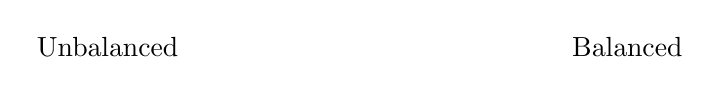
\begin{tikzpicture}
      \DSPECTRUM{4}{2}{1}
      \draw (-1.5,.5) node[align=right] {Unbalanced} ++(6.6,0) node[align=left] {Balanced};
    \end{tikzpicture}
  \caption{Visual representation of the equilibrium-state $(2:4)$. The size of the full x-axis is $M=4$ and the length of the bar is $I=2$. The left side of the spectrum is equivalent to the unbalanced equilibrium-state, and the right the balanced state.}\label{fig:eqstate}
\end{figure}
For example, a cluster with $M=4$ requires 4 growth iterations to reach an equilibrium in potential matching weight in all nodes in the cluster. The equilibrium-state thus gives us an indication of how near balanced-bloom a cluster performs. 
\begin{lemma}\label{lem:parityinversion}
  Let $(I_t, M_t)$ denote the equilibrium-state of a cluster just before a union with another cluster that causes a parity inversion, and $(I_{t+1}, M_{t+1})$ the equilibrium-state after the union, then $I_t \propto M_{t+1}$.
\end{lemma}
\begin{proof}
  In the context of the equilibrium-state, the delayed bloom of nodes in cluster growth is equivalent to increasing the value of $I$ in the equilibrium-state. As $I_t\to M_t$, the difference between the radii of the prioritized and delayed nodes increases, thus also increases the iterations $M_a$ needed after the union and parity inversion. 
\end{proof}
Subsequent parity inversions cause a gradual but certain increase in $M$ of the equilibrium-state, depending on $(I_t:M_t)$ during the parity inversion at the union, requiring a growing number of growth iterations $I_{t+1}$ to reach the equilibrium-state $(M:M)_{t+1}$. As the lattice size is increased, the total number of unions of a cluster with other clusters also increases, leading to a growing number of parity inversions. Thus increasing the lattice size has the consequence that more growth iterations $I$ are needed to reach equilibrium-state $(M:M)$. This is the trade-off in the effectiveness of this algorithm. On the one hand, it is preferred that $I\to M$ to maximally occupy the equilibrium-state that is a heuristic for minimum-weight, but on the other, $I$ is also proportional to the number of iterations needed to actually reach $(M:M)$ due to parity inversions. 

\begin{definition}
  Let the \emph{equilibrium factor} $\gls{zkeq}\in [0,1]$ be a target factor to the node delay. 
\end{definition}
\begin{lemma}
  The delay equation where the delays have a factor $k_{eq}\in [0,1]$ minimizes the trade-off caused by parity inversion. 
  \begin{multline}
    s_\beta.d = s_\alpha.d + \Bigg \lceil k_{eq} \Bigg( 2\bigg(\ceil{\frac{s_\beta.r}{2}} - \floor{\frac{s_\alpha.r + s_\beta.r \bmod 2}{2}} - (-1)^{s_\beta.p}\abs{(s_\beta,s_\alpha)}\bigg)
    \Bigg) - \\
    (s_\beta.r - s_\alpha.r) \bmod 2 \Bigg \rceil \hspace{1em} | \hspace{1em} s_\beta \neq s_r. \tag{\ref{eq:delayequation}}
  \end{multline}
\end{lemma}
\begin{proof}
  For any $k_{eq} < 1$, a cluster will never actually reach the $(M:M)$ equilibrium-state, only $(k_{eq}M:M)$. Let the equilibrium-state with the equilibrium-state be thus be defined as $(I:k_{eq}M)$. Consequently, after a parity inversion, the difference in node radii between prioritized and delayed nodes is decreased, such $I\to k_{eq}M$ can be reached in a lower amount of growth iterations. 
\end{proof}

In Figure \ref{fig:kbloom} and \ref{fig:kbloom2}, a comparison is made between the growth of a set of node-trees using Equation \eqref{eq:delayequation} with $k_{eq}=1$ (same as Equation \eqref{eq:2ddelay}) and with $k_{eq}=1/2$. We see that the number of iterations needed to maximally occupy the equilibrium state using $k_{eq}$ is halved before and after the union with parity inversion when using $k_{eq} = 1/2$. 

The optimal value of $k_{eq}$ may be dependent on the number of parity inversions, the lattice size, growth iteration, and the node-tree and cluster sizes $|\nset|, |\vset|$, with the goal of maximally occupying the equilibrium-state after the last parity inversion. We suspect that because $M$ doubles after parity inversion, a constant factor of $k_{eq}=1/2$ should behave well on average, as the equilibrium state is occupied half on average. However, other values of $k_{eq}$ should be explored, and optimizations dependent on these variables could be possible. 

\tikzstyle{edge}=[above,midway,font=\tiny]
\newcommand\DLINE[4]{
  \draw (#1, #2) ++ (-.3,-.9) node[inner sep=0] (lb) {} ++(#3,0) ++(.6,0) node[inner sep=0] (rb) {} ++(0,0.4) node[inner sep=0] (rt) {};;
  \path[fill=white!80!black, rounded corners=2pt] (lb) rectangle (rt);
  \ifnumequal{#4}{1}{\draw[thin] (lb) -- (rb);}{}
}
\begin{figure}[htbp]
\centering
    \begin{tikzpicture}[on grid, scale=1]
      \foreach \x in {0,3,6}{\DLINE{\x}{0}{2}{1}}
      \foreach \x in {0,2,3,5,6,8}{\draw (\x,0) node [even] (a\x) {1} ++(0,-.7) node (ad\x) {0};}
      \foreach[count=\i] \x in {1,4,7}{      \draw (\x,0) node [odd]  (a\x) {1} ++(0,-.7) node (ad\x) {2};
                                             \node at (\x,0.7) {$\nset_\i$};}
      \foreach \x in {0.5,3.5,6.5}{\DSPECTRA{2}{0}{\x}{-1.5}{0.3}{0.5}}
      \draw[l1] (a0) -- (a1) node[edge]{1} -- (a2) node[edge]{1} (a3) -- (a4) node[edge]{1} -- (a5) node[edge]{1} (a6) -- (a7) node[edge]{1} -- (a8) node[edge]{1};

      \begin{scope}[shift={(0,-3)}]
      \foreach \x in {0,3,6}{\DLINE{\x}{0}{2}{0}}
      \foreach \x in {0,2,3,5,6,8}{\draw (\x,0) node [even] (e\x) {2} ++(0,-.7) node {0};}
      \foreach \x in {1,4,7}{      \draw (\x,0) node [odd]  (e\x) {1} ++(0,-.7) node {1};}
      \foreach \x in {0.5,3.5,6.5}{\DSPECTRA{2}{1}{\x}{-1.5}{0.3}{0.5}}
      \draw[l1] (e0) -- (e1) node[edge]{1} -- (e2) node[edge]{1} (e3) -- (e4) node[edge]{1} -- (e5) node[edge]{1} (e6) -- (e7) node[edge]{1} -- (e8) node[edge]{1};
      \draw[l1, dashed] (e2) -- (e3) (e5) -- (e6);
      \end{scope}

      \begin{scope}[shift={(0,-6)}]
      \DLINE{0}{0}{8}{1}
      \foreach \x in {0,2,6,8}{\draw (\x,0) node [even] (b\x) {2} ++(0,-.7) node {0};}
      \foreach \x in {1,7}{    \draw (\x,0) node [odd]  (b\x) {1} ++(0,-.7) node {1};}
      \foreach \x in {3,5}{    \draw (\x,0) node [odd]  (b\x) {2} ++(0,-.7) node {4};}
                               \draw (4,0)  node [even] (b4)  {1} ++(0,-.7) node {1};
      \DSPECTRA{4}{0}{3}{-1.5}{0.3}{0.5}
      \draw[l1] (b0) -- (b1) node[edge]{1} -- (b2) node[edge]{1} -- (b3) node[edge]{2} -- (b4) node[edge]{1} -- (b5) node[edge]{1} -- (b6) node[edge]{2} -- (b7) node[edge]{1} -- (b8) node[edge]{1};
      \end{scope}

      \node[anchor=east, align=right] at (-1,0) {$n_i.s$};
      \node[anchor=east, align=right] at (-1,-0.75) {$n_i.d$};
      \node[anchor=east, align=right] at (-1,-1.5) {$(I:M)$};
      \path (-3,-3) node[even]{} -- +(.5,0) node[anchor=west] {$n.p$ even}; 
      \path (-3,-4) node[odd]{} -- +(.5,0) node[anchor=west] {$n.p$ odd}; 
      \draw[semithick, ->] (9,-.75) to [out=-60, in=60] ++(0,-2.5);
      \draw[semithick, ->] (9,-3.75) to [out=-60, in=60] ++(0,-2.5);
      \node at (10, -2) [align=right, text width = 3cm] {\underline{PDC}, \codefunc{Grow}};
      \node at (10, -5) [align=right, text width = 3cm] {\codefunc{Join}, \underline{PDC}};

%       \draw[l1, ->] (a8) ++(1,-.35) -- +(0,-2) node[midway, right, text width = 5cm, align=left] {Grow and calculate \\delay with eq. \eqref{eq:2ddelay}};
%       \draw[l1, ->] (c8) ++(1,-.35) -- +(0,-2) node[midway, right, text width = 5cm, align=left] {Grow and calculate \\delay with eq. \eqref{eq:delayequation},\\ $K_{bloom} = 0.5$};
    \end{tikzpicture}
    \caption{The delay values $n_i.d$ and the equilibrium-states $(I:M)$ for 3 odd clusters $\{\nset_1, \nset_2, \nset_3\}$ of 3 nodes that grow and join into a size-9 cluster. Initially (top), parity and delay calculations (PDC) are performed with delay equation \eqref{eq:2ddelay} on each odd cluster which have equilibrium-states $(0:2)$, with delay $2$ in the middle node. The clusters are grown (middle), where the middle node is delayed, such that it's delay value decreases to $1$, and the clusters have equilibrium-states $(1:2)$. The clusters join (bottom) to a single odd cluster, which is selected for growth. Hence PDC is performed again, and the equilibrium-state is $(0:4)$, thus requiring 4 growth iterations before equal potential matching weight is reached in all nodes.}\label{fig:kbloom}
\end{figure}

\begin{figure}[htbp]
  \centering
  \begin{tikzpicture}
      \foreach \x in {0,3,6}{\DLINE{\x}{0}{2}{1}}
      \foreach \x in {0,2,3,5,6,8}{\draw (\x,0) node [even] (c\x) {1} ++(0,-.7) node {0};}
      \foreach[count=\i] \x in {1,4,7}{      \draw (\x,0) node [odd]  (c\x) {1} ++(0,-.7) node (cd\x) {2};
                                             \node at (\x,0.7) {$\nset_\i$};}
      \foreach \x in {.75,3.75,6.75}{\DSPECTRA{1}{0}{\x}{-1.5}{0.3}{0.5}}
      \draw[l1] (c0) -- (c1) node[edge]{1} -- (c2) node[edge]{1} (c3) -- (c4) node[edge]{1} -- (c5) node[edge]{1} (c6) -- (c7) node[edge]{1} -- (c8) node[edge]{1};

      \begin{scope}[shift={(0,-3)}]
      \foreach \x in {0,3,6}{\DLINE{\x}{0}{2}{0}}
      \foreach \x in {0,2,3,5,6,8}{\draw (\x,0) node [even] (c\x) {2} ++(0,-.7) node {0};}
      \foreach \x in {1,4,7}{      \draw (\x,0) node [odd]  (c\x) {1} ++(0,-.7) node {0};}
      \foreach \x in {.75,3.75,6.75}{\DSPECTRA{1}{1}{\x}{-1.5}{0.3}{0.5}}
      \draw[l1] (c0) -- (c1) node[edge]{1} -- (c2) node[edge]{1} (c3) -- (c4) node[edge]{1} -- (c5) node[edge]{1} (c6) -- (c7) node[edge]{1} -- (c8) node[edge]{1};
      \draw[l1, dashed] (e2) -- (e3) (e5) -- (e6);
      \end{scope}

      \begin{scope}[shift={(0,-6)}]
      \DLINE{0}{0}{8}{1}
      \foreach \x in {0,2,6,8}{\draw (\x,0) node [even] (d\x) {2} ++(0,-.7) node {0};}
      \foreach \x in {1,7}{    \draw (\x,0) node [odd]  (d\x) {1} ++(0,-.7) node {0};}
      \foreach \x in {3,5}{    \draw (\x,0) node [odd]  (d\x) {2} ++(0,-.7) node {2};}
                               \draw (4,0)  node [even] (d4)  {1} ++(0,-.7) node {0};
      \draw[l1] (d0) -- (d1) node[edge]{1} -- (d2) node[edge]{1} -- (d3) node[edge]{2} -- (d4) node[edge]{1} -- (d5) node[edge]{1} -- (d6) node[edge]{2} -- (d7) node[edge]{1} -- (d8) node[edge]{1};
      \DSPECTRA{2}{0}{3.5}{-1.5}{0.3}{0.5}
      \end{scope}

      \node[anchor=east, align=right] at (-1,0) {$n_i.s$};
      \node[anchor=east, align=right] at (-1,-0.75) {$n_i.d$};
      \node[anchor=east, align=right] at (-1,-1.5) {$(I:M)$};
      \path (-3,-3) node[even]{} -- +(.5,0) node[anchor=west] {$n.p$ even}; 
      \path (-3,-4) node[odd]{} -- +(.5,0) node[anchor=west] {$n.p$ odd}; 
      \draw[semithick, ->] (9,-.75) to [out=-60, in=60] ++(0,-2.5);
      \draw[semithick, ->] (9,-3.75) to [out=-60, in=60] ++(0,-2.5);
      \node at (10, -2) [align=right, text width = 3cm] {\underline{PDC}, \codefunc{Grow}};
      \node at (10, -5) [align=right, text width = 3cm] {\codefunc{Join}, \underline{PDC}};

  \end{tikzpicture}
  \caption{The same clusters, growths and joins as in Figure \ref{fig:kbloom}, but now with delay equation \eqref{eq:delayequation} for $f_{eq} = 1/2$. With the equilibrium factor, $(f_{eq}M:M)$ can be reached in fewer growth iterations; e.g. after 1 round (middle), $(1:1)$ is reached. Also after join to a single cluster (bottom), fewer iterations are needed (2 compared to 4 in Figure \ref{fig:kbloom}).}\label{fig:kbloom2}
\end{figure}
 
\subsection{Parity and delay calculations}\label{sec:pdccalc}

With equation \eqref{eq:nodeparity} and \eqref{eq:delayequation}, we now finally have the tools to formulate the algorithms to calculate the node parities and delays. For a node-tree with root $n_r$, we can calculate the parities by calling the \emph{head recursive} function \codefunc{Calcparity} on $n_r$ in Algorithm \ref{algo:calcparity}, where we do a reverse DFS of the node-tree. The node delays are calculated by calling the \emph{tail recursive} function \codefunc{Calcdelay} in Algorithm \ref{algo:calcdelay}, where we perform a second DFS of the node-tree. This parity and delay calculation will from this point sometimes be abbreviated as PDC. A schematic of the directions of these calculations in an example node-tree is included in Figure \ref{fig:2dfs}.

\begin{algorithm}[htbp]
  \SetKwFunction{cp}{Calcparity}
  \SetKwFunction{summation}{Sum}
  \KwData{Node $n$}
  \KwResult{Calculated parities for $n$ and all its descendent nodes}
  \BlankLine
  parity $=$ \summation{$[1 - $ \cp{$n_\gamma$} $\forall$ children $n_\gamma$ of $n]$} $\bmod 2$\;
  \uIf{$n \equiv s$}{
      $n.p =$ parity}
  \uElseIf{$n \equiv l$}{
      $n.p= 1-$ parity}
  \KwRet{$n.p$}
  \caption{\codefunc{Calcparity}}\label{algo:calcparity}
\end{algorithm}

\begin{algorithm}[htbp]
    \SetKwFunction{cdelay}{Calcdelay}
    \KwData{Node $n$, cluster $c$}
    \KwResult{Calculated delays for $n$ and all its descendent nodes}

    \BlankLine
    \If{$n$ has a parent}{
        calculate $n.d$ with equation \eqref{eq:delayequation} using $n$ and $n.parent$\;
        \If{$n.d < c.d$}{
            $c.d=n.d$
        }
    }
    \For{children $n_\gamma$ of $n$}{
        \cdelay{$n_\gamma, c$}
    }
    \caption{\codefunc{Calcdelay}}\label{algo:calcdelay}
\end{algorithm}

\begin{figure}[htbp]
  \centering
  \begin{tikzpicture}[x=1.5cm,y=1.5cm]
    \node[node1,even] (a) at (1, 3) {$n_r$};
    \node[node1,odd]  (b) at (1, 2) {};
    \node[node1,odd]  (c) at (1, 1) {};
    \node[node1,even] (d) at (1, 0) {};
    \node[node1,even] (e) at (0, 1) {};
    \node[node1,even] (f) at (0, 0) {};
    \node[node1,odd]  (g) at (2, 2) {};
    \node[node1,even] (h) at (2, 1) {};
    \node[node1,even] (i) at (2, 0) {};
    \draw[l1] (a) -- (b) -- (c) -- (d);
    \draw[l1] (b) -- (e);
    \draw[l1] (c) -- (f);
    \draw[l1] (c) -- (i);
    \draw[l1] (a) -- (g) -- (h);

    \draw[l1, ->, dashed, color=mblue] (0, 1.3) -- +(45:0.85) arc (-45:0:.5) -- +(90:.6);
    \draw[l1, ->, dashed, color=mblue] (0, 0.3) -- +(45:0.85) arc (-45:0:.5) -- +(90:.2);
    \draw[l1, ->, dashed, color=mblue] (0.75,0.2) -- +(90:.3);
    \draw[l1, ->, dashed, color=mblue] (1.5,0.2) -- +(135:.4);
    \draw[l1, ->, dashed, color=mblue] (1.75,1.2) -- +(90:0.5) arc (0:45:.5) -- +(135:0.4);
    \draw[l1, ->, color=mred] (1.4, 3) -- +(-45:1.1) arc (45:0:0.5) -- +(-90:0.7);
    \draw[l1, ->, color=mred] (1.3, 2.1) -- +(-90:0.9) arc (180:225:.5) -- +(-45:0.7);
    \draw[l1, ->, color=mred] (0.6, 1.3) -- +(225:.3);
    \draw[l1, ->, color=mred] (0.6, 0.3) -- +(225:.3);
    \draw[l1, ->, color=mred] (1.3, 0.3) -- +(-90:.2);
    \node[text=mblue] at (0,2.2) {Parity};
    \node[text=mred] at (2.6,2.8) {Delay};
    \node at (0,3) {$\mathcal{N}$};
    \path (4,3) node[node1, even]{} -- +(.5,0) node[anchor=west] {$n.p$ even}; 
    \path (4,2.5) node[node1, odd]{} -- +(.5,0) node[anchor=west] {$n.p$ odd}; 
  \end{tikzpicture}
  \caption{The parity and delay calculation performed from a the root node $n_r$, which is equivalent to two depth-first searches on $\mathcal{N}$ to compute node parities (head recursively) and delays (tail recursively).}\label{fig:2dfs}
\end{figure}

\section{Growing a cluster}\label{sec:growingcluster}
With the knowledge of the previous section, we now have the equations and algorithms available to describe the steps to grow a cluster in the context of Union-Find Balanced-Bloom. Previously, in the Union-Find decoder, a cluster is grown with $\codefunc{Grow}(c_j, \m{L}_m)$ (Algorithm \ref{algo:ufgrow}). Here, the boundary edges connected to the vertices in $c_j.\delta\vset$ are grown by increasing the value of $e.support$. If $e.support = 2$, $e$ is added to the merging list $\m{L}_m$ to merge the vertex-trees at some later moment. 

In the node-tree data structure, the growth of a cluster is equivalent to a depth-first search of the node-tree, which will now be performed by $\codefunc{Ngrow}$ (Algorithm \ref{algo:bbgrow}). The boundary list for each cluster is not stored at the cluster $c_j$, but separately stored at each of the nodes $n_i$ in $\m{N}_j$ by $n_i.\delta\vset$. We travel to all $n_i \in \m{N}_j$ from the root $n_r$ and apply $\codefunc{Bloom}(n_i)$ (Algorithm \ref{algo:bloom}), which grows the boundaries for each node individually. Again, if an edge on the boundary are grown to $e.support = 2$, $e$ is added to the merging list $\m{L}_m$. Elements of $\m{L}_m$ are then iterated over to merge the vertex-trees and node-trees at some later moment. The merging of node-trees is considered in Section \ref{sec:nodejoin}. 

Recall from Theorem \ref{def:balancedbloom} that with Balanced-Bloom, the bloom of node with the lowest potential matching weight in the cluster are prioritized, whereas the bloom of other nodes are delayed. Also, from Lemma \ref{lem:calconce}, in the absence of unions, the delays are not recalculated after every growth iteration, but stored in memory at the nodes. Definition \ref{def:absolutedelay} introduced the absolute delay $n_i.D$, where the actual number of iterations to delay is updated via the minimal delay value $c_j.d$ in the cluster, and the number of iterations already waited for $n.w$. Thus, when performing the depth-first search in \codefunc{Ngrow}, a node should be conditionally bloomed if only $n_i.D = 0$ is satisfied. If not, node $n_i$ is skipped, the wait $n.w$ is increased, and the depth-first search continues recursively on its children nodes. 

\begin{algorithm}[htbp]
    \BlankLine
    \KwData{Node $n$, merging list $\m{L}_m$}
    \KwResult{Node with traced boundary edges and increased radius}
    \BlankLine
  
    \For{$v$ in $n_i.\delta\vset$}{
      \For{edges in $\{(u,v) | (u,v).support\neq 2$\}}{
        Add 1 to $(u,v).support$ \;
        If $(u,v).support=2$, add $(u,v)$ to $\m{L}_m$ \;
      }
    }
    Add 1 to $n.r$ \tcp*{Node has increased in radius}
    \BlankLine
    \caption{\codefunc{Bloom}}\label{algo:bloom}
  \end{algorithm}
\begin{algorithm}[htbp]
    \SetKwFunction{grow}{Ngrow}
  
    \KwData{Node $n$, cluster $c_j$, merging list $\m{L}_m$}
    \KwResult{A node that has either grown or waited one iteration.}
  
    \BlankLine
  
    \eIf{$n.d-n.w-c_j.d=0$}{
      \codefunc{Bloom}$(n, \m{L}_m)$ (Algorithm \ref{algo:bloom})\; 
    }{
      Add 1 to $n.w$ \tcp*{Let the node be delayed for one iteration}
    }
    \For{child node $n_\gamma$ of $n$}{
      \grow{$n_\gamma$} \tcp*{Recursively applies to all descendant nodes}
    }
    \caption{\codefunc{Ngrow}}\label{algo:bbgrow}
  \end{algorithm}
  

\section{Joining node-trees}\label{sec:nodejoin}
Within the vertex-tree $\m{V}$, which utilizes the Union-Find data structure, \emph{path compression} and \emph{union by weight} or \emph{union by rank} are applied to minimize the depth of the tree. These rules minimize the calls to the \codefunc{Find} function. Similarly, in the node-tree $\m{N}$, we would also like to apply a set of rules to reduce the calls to \codefunc{Calcparity} and \codefunc{Calcdelay}, which we will dub the parity and delay calculation minimization.

\begin{definition}\label{def:partialpdc}
  A partial parity or partial delay calculation, which will often be abbreviated to a partial calculation, is associated with a depth-first search that is not initiated from the root node $n_r$, but some descendant node of $n_r$ in the node-tree. 
\end{definition}

This minimization is achieved by preserving the node parities and delays in subsets of the merged node-tree after union, and applying a partial calculation of the parities and delays in the remaining subsets if required. The recursiveness of both \codefunc{Calcparity} and \codefunc{Calcdelay} (Algorithms \ref{algo:calcparity} and \ref{algo:calcdelay}) ensures that this is possible. The tail-recursive parity calculation stops at the node where the depth-first search is started, and the head-recursive delay calculation now has a non-arbitrarily node delay. 

With the addition of the node-tree data structure, during the merge of clusters $c_\alpha$ and $c_\beta$, we have to additionally merge the node-trees $\m{N}_{\alpha}$ and $\m{N}_\beta$ that require its own set of rules that we will explain in this section. Let us first make a clear distinction between the various methods. For the merge of vertex-trees $\vset_\alpha, \vset_\beta$ we apply $\codefunc{Union}(v_\alpha, v_\beta)$ (Algorithms \ref{algo:unionweight} or \ref{algo:unionrank}), with the two vertices spanning the edge connecting two clusters as arguments. For the merge of node-trees $\nset_\alpha, \nset_\beta$, we introduce here $\codefunc{Join}(n^\alpha, n^\beta)$ (Algorithm \ref{algo:join}), which is called on the two nodes $n_\alpha, n_\beta$ that seed vertices $v^\alpha, v^\beta$, respectively. During a merge of two clusters, these routines are both applied to their respective sets. Within the context of the Union-Find Balanced-Bloom decoder, when either one of the expressions ``merge clusters $C_\alpha$ and $C_\beta$'', ``the union of vertex-trees $\m{V}_\alpha$ and $\m{V}_\beta$'' or the ``join of node-trees $\m{N}_{\alpha}$ and $\m{N}_\beta$'' is mentioned, it is always implied that both routines are executed.

\begin{definition}\label{def:nodesetparity}
  Let the parity of a node-tree be the number of syndrome-nodes in the node-tree modulo 2. The parity of the node-tree is thus equivalent to the parity of its cluster. 
\end{definition}
\begin{definition}\label{def:oddevenjoin}
  Let us categorize the joins of two node-trees into two types: even-joins and odd-joins, depending on the parity of the node-tree after the join. An even-join may be the result of the join of two even node-trees or two odd node-trees, whereas an odd-join is the result of the join of one odd node-tree and one even node-tree.
\end{definition}

% Only odd clusters with odd parity node-trees are grown in the Union-Find decoder. It may thus be tempting to conclude that a join must include at least one odd node-tree. This is however not true as within the same growth iteration, there may be many joins, where some odd cluster $\nset_1^o$ first joins with odd cluster $\nset_2^o$, but also joins with even cluster $\nset_3^e$. The second join is effectively between even clusters. Hence there are 3 types of joins: 1) odd-odd, 2) even-odd and 3) even-even, where even-odd is equivalent to odd-even. These joins can be put into 2 \emph{classes}, dependent on the parity of the resulting cluster. Both odd-odd and even-even joins to an even cluster and thus belongs to the even class join (E-join), whereas even-odd (and odd-even) joins to an odd cluster in the odd class join (O-join).

\begin{lemma}\label{lem:nodecalc_even}
  If node-trees merge into an even node-tree $\nset^e$, all node parities and delays within $\nset^e$ become invalid or \emph{undefined}. 
\end{lemma}
\begin{proof}
  Recall from Definitions \ref{def:nodeparity} and \ref{def:nodedelay} that the node parity and delay are only defined for odd-parity clusters. An even-parity cluster does not have a potential matching weight, as the matching within the cluster is already defined. However, $\nset^e$ can merge with another odd-parity cluster with node-tree $\nset^o$ in a larger odd-join. In that case, we might think about ``reusing'' some node parities and delays that were already calculated in $\nset^e$. To reuse prior calculated parities and delays, a depth-first search on $\nset^e$ is needed to find which sections are still valid, and which sections are not. This is especially the case when the clusters in the E-join are the results of joins within the same growth iteration. Checking the validity to reuse prior parities and delays then acquires the same complexity as redoing the calculation of parity and delays over the subtree $\nset^e$. Hence, the node parities and delays in the joined set after an E-join are \emph{undefined}.
\end{proof}

\begin{lemma}\label{lem:nodecalc_odd}
  Consider an odd-join on nodes $n_j^e \in \nset^e, n_j^o\in \nset^o$, belonging to an even and an odd node-tree, respectively. Parity and delay calculations are minimized if the node-trees are always joined by setting $n_j^e$ as the child of $n_j^o$. 
\end{lemma}
\begin{proof}
  If $n_j^e$ is made a child of $n_j^o$, $n_j^e$ is the new subroot of subtree $\nset^e$, and an even number of syndrome-nodes are now descendants of $n_j^o$, and parities within $\nset^o$ and its root are unchanged. Recall from Lemma \ref{lem:nodecalc_ancestrypath} that thus the delays in $\nset^o$ are also unchanged. A partial parity and delay calculation can now be initiated from $n_j^e$ and is proportional to $|\nset^e|$ (Figure \ref{fig:joinrules}b). If $n_j^o$ is made a child of $n_j^e$, an odd number of syndrome-nodes are descendants of $n_j^e$ and change the parities in the ancestors of $n_j^o$ up to the root of the joined tree. The parities and delays now need to be recalculated in the entire tree, which is proportional to $|\nset^e| + |\nset^o|$ (Figure \ref{fig:joinrules}c). 
\end{proof}

\begin{figure}[htbp]
    \centering
    \begin{tikzpicture}[on grid]
      \node (o1) [even] at (1.5, 1) {$s_1$};
      \node (o2) [even] at (1, 0) {$s_2$};
      \node (o3) [even] at (2, 0) {$s_3$};
      \node (e4) [undef] at (3.5,1) {$s_4$};
      \node (e5) [undef] at (3.5,0) {$s_5$};
      \draw[l1] (o2) -- (o1) -- (o3) (e4) -- (e5);
      \draw[l1, dashed] (o3) -- (e) node[midway,below] (a) {};
      \draw[l1, <-] (a) -- ++(0,-.5) node[below] {$\codefunc{Join}(s_3, s_5)$};
    
      \begin{scope}[shift={(4.5,1)}]
      \node (o1) [even] at (1.5, 1) {$s_1$};
      \node (o2) [even] at (1, 0) {$s_2$};
      \node (o3) [even] at (2, 0) {$s_3$};
      \node (e4) [undef] at (2,-2) {$s_4$};
      \node (e5) [undef] at (2,-1) {$s_5$};
      \draw[l1] (o2) -- (o1) -- (o3) -- (e5) -- (e4);
      \draw[l1, ->, dashed, color=mblue] (e4) ++(-.7,0) -- + (0,1);
      \draw[l1, ->, color=mred] (o3) ++(.7,-.5) -- +(0,-1.5);
      \end{scope}
    
      \begin{scope}[shift={(9,1.5)}]
      \node (o1) [undef] at (1, -2) {$s_1$};
      \node (o2) [undef] at (1, -3) {$s_2$};
      \node (o3) [undef] at (1, -1) {$s_3$};
      \node (e4) [undef] at (1,1) {$s_4$};
      \node (e5) [undef] at (1,0) {$s_5$};
      \draw[l1] (o2) -- (o1) -- (o3) -- (e5) -- (e4);
      \draw[l1, ->, dashed, color=mblue] (o2) ++(-.7,0) -- +(0,4);
      \draw[l1, ->, color=mred] (e4) ++(.7,0) -- +(0,-4);
      \end{scope}
    
      \node at (1,2) {\emph{(a)}};
      \node at (4,2) {\emph{(b)}};
      \node at (8.5,2) {\emph{(c)}};
      \path (12.5, 2) node[even] {} -- +(.5,0) node[anchor=west]{$n.p$ even};
      \path (12.5, 1) node[undef] {} -- +(.5,0) node[anchor=west]{$n.p$ undefined};
      \draw[l1, ->, color=mred] (12.25, -1) -- ++(0.5,0);
      \node[color=mred, anchor=west] at (13,-1) {Calcdelay};
      \draw[l1, ->, color=mblue, dashed] (12.25, 0) -- ++(0.5,0);
      \node[color=mblue, anchor=west] at (13,0) {Calcparity};
    \end{tikzpicture}
    \caption{(a) An odd cluster $\nset^o=\{s_1, s_2, s_3\}$ with root $n^o_r = s_1$ joins with an even cluster $\nset^e=\{s_4, s_5\}$ with root $n^e_r=s_4$ on nodes $s_3, s_5$, respectively, to a new set $\nset$ with subsets $'\nset^e$ and $'\nset^o$.  If we choose to (b), make $s_5$ a child of $s_3$, the parities and delays in $'\nset^o$ can be reused, and we only have perform partial parity and delay calculations over $'\nset^e$. If we choose to (c), make $s_3$ a child of $s_5$, parities and delays have to be recalculated over both $'\nset^2e$ and $'\nset^o$}\label{fig:joinrules}
\end{figure}
% \subsection{O-joins}\label{sec:ojoin}

% Consider now an O-join between an even node-tree $\m{N}^e$ and an odd node-tree $\m{N}^o$ in nodes $n^e, n^o$ respectively, and assume that this join is due to the growth of odd cluster $\m{N}^o$ onto an ``idle'' $\m{N}^e$. The join of these two sets produces a new odd node-tree $\m{N}_{new}^o$ with subsets $'\nset^e$ and $'\nset^o$, referring to the original node-trees. We are provided with two choices, A) make $n^e$ child of $n^o$, or B) make $n^o$ child of $n^e$. The ancestry in the parent node-tree stays unchanged, but the ancestry in the child subset is changed by setting the joining node in the child set $n^c$ as the subroot of the child subset $'\m{N}^c$. This is allowed per Lemma \ref{lem:anynoderoot}, but removes any calculated parities or delays per Lemma \ref{lem:anynoderoot} and \ref{lem:nodecalc_ancestrypath}.

% For option A, an even number of nodes of $'\m{N}^e$ is attached to $n^o$, and the ancestry in $'\m{N}^o$ hasn't changed. The parities and delays in $'\m{N}^o$ stay valid and can be reused. From $n^e$, which is now the subroot of  $'\m{N}^e$, a partial PDC is applied, where the relative delay of $n^e$ is calculated with respect to its parent $n^o$ (Figure \ref{fig:joinrules}A). This is efficient as the parities and delays in $'\m{N}^e$ are already undefined per Lemma \ref{lem:nodecalc_even}. For option B, we need to redo the PDC in both $'\m{N}^o$ and $'\m{N}^e$ (Figure \ref{fig:joinrules}B), as $'\m{N}^o$ has a changed ancestry and  $'\m{N}^e$ is even. The PDC is thus minimized if option A is always chosen. \\

% If the subset $'\m{N}^e$ consists of only two odd node sub-subsets $''\m{N}^o_0, ''\m{N}^o_1$, where $n_0, n_1$ are the joining nodes, the ancestry in $''\m{N}^o_0$ is preserved and $n_1$ is the subroot of $''\m{N}^o_1$. We see that the parities in all ancestors of $n_0$ are flipped. Let's consider the cases and find whether we can minimize the parity and delay calculation in $'\m{N}^{e}$.
%
% For case a), an even number of nodes of $'\m{N}^e$ is attached to $n^o$, and the ancestry in $'\m{N}^o$ hasn't changed. This means that the parities in $'\m{N}^o$ do not change per Lemma \ref{lem:anynoderoot}, and the delays in $'\m{N}^o$ are still valid as per Lemma \ref{lem:nodecalc_ancestrypath}. In $'\m{N}^e$, as the ancestry path has changed, we are certain to traverse $'\m{N}^e$ from the subroot $n^e$ to calculate the delays in this subset which is in the order of $S_{'\m{N}^e}$.
%
% In case b), as an odd number of nodes of $'\m{N}^o$ is attached to $n^e$, it means that parities of all ancestor of $n^e$ are flipped. As the ancestry in $'\m{N}^{o}$ has changed, we are certain to traverse $'\m{N}^o$ from the subroot $n^o$ to calculate the delays which is in the order of $S_{'\m{N}^o}$. The node parity changes in $'\m{N}^e$ will be dependent on the location of $n^e$ in the ancestry compared to $n^1$ and $n^2$, and all children nodes of these parity changes will have to recalculate their delays. Let's call the number of nodes needs to calculate parity and delays in $'\m{N}^e$ a value $S_e \leq S_{'\m{N}^e}$, leaving the total number of operations in the order of $S_e + S_{'\m{N}^o}$.
%
% For $'\m{N}^e$ consisting of two subsets, keeping track of the parity changes between $n^e$, $n^0$ and $n^1$ is still an easy task, and we might gain in minimization in operations in case b) compared to case a) for some value $S_e$ such that $S_e + S_{'\m{N}^o} < S_{'\m{N}^e}$. But as the number of subsets in $'\m{N}^e$ increases, the task of finding the ancestry paths of parity changes becomes analogous to traversing $'\m{N}^e$ entirely $S_e \rightarrow S_{'\m{N}^e}$. To simplify, we always choose case a.

From Lemmas \ref{lem:nodecalc_even} and \ref{lem:nodecalc_odd}, we can define a simple rule that determines how node-trees are joined.

\begin{definition}\label{def:joinbyparity}
  Let the \emph{join by parity} rule govern how to join node-trees in the event of clusters merging. For even-joins between two even or two odd node-trees, the parent and child node-trees can be picked at random. For odd-joins between nodes $n_j^e \in \nset^e, n_j^o \in \nset^o$, always make the even node-tree a child of the even node-tree, where $n_j^e$ is now the subroot of the subtree $\nset^e$.
\end{definition}
The \emph{join by parity} rule ensures that the parities and delays in $\nset^o$ are preserved and that only a partial calculation is needed equivalent to the depth-first search from node $n_j^e$. Note the concept of a \emph{partial} calculation is somewhat redundant. Using these rules for the joins of node-trees, the parity and delay calculations are never calculated on a full node-tree, except for the initial round. 

Recall from Definition \ref{def:nodeset} that the node-tree $\nset_j$ of cluster $c_j$ is stored as its root node at $c_j.n_r$, which sets the ancestry in the node-tree. In a join of two node-sets, the \emph{join by parity} rule requires to conditionally set the ancestry in the joined node-set. This can simply be done by connecting the node-trees with a new edge selecting the correct root node to be stored in the merged cluster (see Algorithm \ref{algo:join}). Also, due to the use of undirected edges, it is required to store the direction of the partial parity and delay calculation.

% \begin{theorem}\label{the:nodejoint}
%   The union of node-trees $\m{N}^\alpha, \m{N}^\beta$ on nodes $n^\alpha, n^\beta$ respectively is performed with $\codefunc{Join}(n^\alpha, n^\beta)$. If the join is between an even and an odd node-tree $\nset^e, \nset^o$ in the nodes $n^e, n^o$, $\codefunc{Join}(n^e, n^o)$ makes the node of the even set $n^e$ a child of the node of the odd set $n^o$. If the join is between two even or two odd node-trees, the choice is arbitrary.
% \end{theorem}
\begin{definition}
  Let us make a distinction between the \emph{final odd-join} between an odd node-tree $'\nset^o$ and an even node tree $'\nset^e$ to a joined node-tree $\nset$, and all others odd-joins that joined to $'\nset^e$ within the same round which we dub \emph{intermediate odd-joins}. 
\end{definition}

\begin{lemma}\label{lem:delaywhengrown}
  Redundant partial parity and delay calculations over even subtrees in intermediate odd-joins are prevented by applying the calculation directly before the growth of the cluster. 
\end{lemma}
\begin{proof}
  Consider the case when partial delay and parity calculations are initiated from a node $n_j^e \in \nset^e \subset \nset$ directly after the join of $\nset^e$ and $\nset^o$ to the joined node-tree $\nset$ while applying the \emph{join by parity} rule of Definition \ref{def:joinbyparity}. If there are many odd-joins (and even-joins) within the same round of growth, that at the end of round all joins to a single cluster with node-tree $\nset$, every odd-join will require the partial calculation over the even subtree. There may thus be many even subtrees where multiple partial calculations are performed within the same round before the final cluster $\nset$ is constructed. All but the final calculation will lead to the correct parities and delays in $\nset$. To circumvent any redundant calculations on the even subtrees of intermediate odd-joins, the partial calculation is suspended as much as possible, until just before a cluster is grown.
\end{proof}

Consider an example with five odd node-trees $\nset_1, ...,  \nset_5$ (Figure \ref{fig:redundantpdc}) that join to a single node-tree, where the partial calculation is applied directly after each join. The join of $\nset_1$ and $\nset_2$ to $\nset_{12}$ is an even-join and requires no partial calculation. The join of $\nset_{12}$ and $\nset_3$ is an odd-join, and we apply partial calculations in $\nset_{12}$. The joining of $\nset_{123}$ and $\nset_4$ is an even-join and the joining of $\nset_{1234}$ and $\nset_5$ is an odd-join, with partial calculations in $\nset_{1234}$. The earlier computation in $\nset_{12}$ is thus redundant. 


\tikzstyle{enset}=[node1, thick, double, font=\footnotesize]
\tikzstyle{onset}=[node1, thick, dotted, double, font=\footnotesize]

\begin{figure}[htbp]
\centering
\begin{tikzpicture}[scale=0.95]
  \node (n1) [onset] at (0,0) {$\nset_1$};
  \node (n2) [onset] at (0,-1) {$\nset_2$};
  \draw[l1, color=orange] (n1) -- (n2);

  \begin{scope}[shift={(2.5,-.5)}]
  \node (n3) [onset] at (0,1) {$\nset_3$};
  \node (n1) [onset] at (0,0) {$\nset_1$};
  \node (n2) [onset] at (0,-1) {$\nset_2$};
  \draw[l1, color=orange] (n3) -- (n1); \draw[l1] (n1) -- (n2);
  \draw[l1, ->, dashed, color=mblue] (n2) ++(-.7,0) -- +(0,1);
  \draw[l1, ->, color=mred] (n1) ++(.7,0) -- +(0,-1);
  \end{scope}

  \begin{scope}[shift={(5.5,-.5)}]
  \node (n3) [onset] at (0,1) {$\nset_3$};
  \node (n1) [onset] at (0,0) {$\nset_1$};
  \node (n2) [onset] at (-.5,-1) {$\nset_2$};
  \node (n4) [onset] at (.5,-1) {$\nset_4$};
  \draw[l1, color=orange] (n1) -- (n4); \draw[l1] (n3) -- (n1) -- (n2);
  \end{scope}

  \begin{scope}[shift={(8.5,-1)}]
  \node (n5) [onset] at (0,2) {$\nset_5$};
  \node (n3) [onset] at (0,1) {$\nset_3$};
  \node (n1) [onset] at (0,0) {$\nset_1$};
  \node (n2) [onset] at (-.5,-1) {$\nset_2$};
  \node (n4) [onset] at (.5,-1) {$\nset_4$};
  \draw[l1, color=orange] (n3) -- (n5); \draw[l1] (n3) -- (n1) -- (n2) (n1) -- (n4);
  \draw[l1, ->, dashed, color=mblue] (n2) ++(-.7,0) -- +(0,2);
  \draw[l1, ->, color=mred] (n3) ++(1.2,0) -- +(0,-2);
  \end{scope}

  \node at (-1, 1) {\emph{(a)}};
  \node at (1.5, 1) {\emph{(b)}};
  \node at (4.5, 1) {\emph{(c)}};
  \node at (7.5, 1) {\emph{(d)}};

  \begin{scope}[shift={(11,1)}]
    \path (0,0)node[onset]{} -- +(.5,0)node[anchor=west]{odd node-tree};
    \draw[l1, ->, color=mred] (-.25, -2) -- ++(0.5,0);
    \node[color=mred, anchor=west] at (.5,-2) {Calcdelay};
    \draw[l1, ->, color=mblue, dashed] (-.25, -1) -- ++(0.5,0);
    \draw[l1, color=orange] (-.25, -3) -- ++(0.5,0);
    \node[color=mblue, anchor=west] at (.5,-1) {Calcparity};
    \node[anchor=west] at (.5,-3) {new edge};
  \end{scope}
\end{tikzpicture}
\caption{If the partial parity and delay calculation is directly performed on the even sub-tree in an odd-join, there may be redundant partial calculations in a series of odd-joins and even-joins within the same growth iteration. Here we picture a series of join events between odd node-trees, where the odd-join in (b) initiates a redundant partial calculation. }\label{fig:redundantpdc}
\end{figure}

% \begin{lemma}\label{lem:oddisevenodd}
%   An odd- node-tree $\nset$ that is the result of some joins must consist of an odd- subtree $'\nset^o$ and an even subtree $'\nset^e$, where the even subtree $'\nset^e$ may consist of smaller sub-subsets $''\nset$.
% \end{lemma}
% \begin{proof}
%   Just like some odd integer $z$ that is the sum of integers $x$ and $y$. If $x$ is odd, then $y$ must be even. This sum can also be of the odd integer $x$ and a set of even integers $\{y_1, y_1, ...\}$. 
% \end{proof}

The only task now is to store the subroot of the even subtree $n_j^e \in '\nset^e$ of the final odd-join, as this subroot is the starting point of the depth-first searches of the partial parity and delay calculation. For every odd-join between odd node-tree $'\m{N}^o$ and even node-tree $'\m{N}^e$ on nodes $'n_j^o, 'n_j^e$ to a cluster $c_j$, store the subroot $'n^e_j$ at the cluster as the \emph{undefined node subroot} $c_j.u$ (Algorithm \ref{algo:join}). If $c_j$ is selected for growth, and has an undefined node subroot $c_j.n_u$, we apply $\codefunc{Calcparity}(c_j.n_u)$ and $\codefunc{Calcdelay}(c_j.n_u)$ (Algorithms \ref{algo:calcparity}, \ref{algo:calcdelay}) to calculate parities and delays in undefined subtrees. We then call $\codefunc{Bloom}(c_j.n_r)$ (Algorithm \ref{algo:bloom}) to grow the cluster. 

% This data structure dynamically saves the root of the undefined part of a cluster to the root node. For any IO-join, we don't know yet whether another O-join will occur, thus each IO-join to cluster $''\nset^o$ is treated as a FO-join. For a IO-join, we thus also store the undefined subroot $u_1$ at the root $R_1=''n_R_{-1}$. If $''\nset^o$ joins with other clusters in subsequent E-join to cluster $'\nset^e$ and lastly the ``real final'' FO-join with $'\nset^o$ to $\nset^o$, we again store the undefined subroot $u_2='n_r^e$ at the new root of $R_2='n_R_{-1}$. Due to Lemma \ref{lem:nodecalc_odd}, it is certain that $u_2$ is an ancestor of $u_1$, and the PDC will traverse over all undefined regions of the set.

% \begin{theorem}\label{the:delayonce}
%   Undefined region of an odd cluster $\nset^o$ is defined as the subroot $u$ for which all children nodes including $u$ have undefined parities and delays, and is stored at root node $n^o_r$. PDC is performed for $n^o_r.u$ and its children before cluster $\nset^o$ is grown.
% \end{theorem}
\begin{algorithm}[htbp]
    \KwData{Merging node $n_i, n_j$ of clusters $c_i, c_j$, merged cluster $c_{ij}$}
    \KwResult{A jointed node tree}
  
    \BlankLine
  
    Merge node sets by initiating edge $(n_i, n_j)$\;
    \uIf{$c_i$ even, $c_j$ odd}{
      set $c_{ij}.n_r = c_j.n_r$\;
      set $c_{ij}.n_u = c_i$
    }
    \uElseIf{$c_i$ odd, $c_j$ even}{
      set $c_{ij}.n_r = c_i.n_r$\;
      set $c_{ij}.n_u = c_j$
    }
    \Else(even-join){
      set $c_{ij}.n_r = c_i.n_r$ or $c_{ij}.n_r = c_j.n_r$\;
    }
    \caption{\codefunc{Join}}\label{algo:join}
  \end{algorithm}
  

\section{Pseudo-code}
Now we have the full description of the modification of the Union-Find decoder, which we dub the \emph{Union-Find Balanced-Bloom} decoder. Recall from Theorem \ref{the:nodepmw} that the potential matching weight is only defined if a dynamic forest of clusters is maintained. Recall also from Section \ref{sec:ufperformance} that weighted growth improves the code threshold of the Union-Find Decoder. Thus, the modification will be applied to the Dynamic-forest Bucket Union-Find decoder \ref{algo:dbuf}. 

In the Union-Find Balanced-Bloom decoder of Algorithm \ref{algo:ufbb}, partial parity and delay calculations are applied if a cluster $c_i$ has an undefined node subroot $c_i.n_u$, and \codefunc{Grow} (Algorithm \ref{algo:ufgrow}) is replaced with \codefunc{Ngrow} (Algorithm \ref{algo:bbgrow}). Furthermore, when iterating over the edges of the merging list $\m{L}_m$, if the vertex-tree roots of the supporting vertices do not belong to the same cluster, it either means that a new vertex is added to the cluster, or that two clusters are merged. In the first case, the new vertex is added to the node, whereas two node-trees are joined in the second case. To differentiate between these cases, we need to additionally store the node $n$ containing the vertex $v\in v.\vset$ at the vertex as $v.n$. With this data structure, two node-trees have to be joined on $v.n$ and $u.n$ if they both exist. Otherwise, the node is to be saved to the newly added vertex. 

\begin{algorithm}[htbp]
  \BlankLine
  \KwData{A graph $G=(\m{V},\m{E})$, an erasure $\m{R} \subseteq \m{E}$ and syndrome $\sigma \subseteq \m{V}$}
  \KwResult{Correction set $\m{C}$}
  \BlankLine
  \tcp{Syndrome validation}
  Initialize clusters $c_i$ with disjoint-set trees $\m{V}_i$, node-trees $\nset_i$ and boundaries at the nodes\;
  Initialize $\m{L}_b$\tcp*{Ensures weighted growth}
  \codefunc{Place} odd-parity clusters in $\m{L}_b$ (Algorithm \ref{algo:place})\;
  \For{bucket $b_k$ in $\m{L}_b$}{
    Initialize $\m{L}_m=\emptyset, \m{L}_p=\emptyset$\;
    \For{$c_i$ in $b_k$}{
      \If{$c_i.bucket$ is $k$}{

        \If{$c_i.r_u$ exists\tcp*{There is a undefined node subroot}}{
          \codefunc{Calcparity}$(c_i.n_u)$ (Algorithm \ref{algo:calcparity})\;
          \codefunc{Calcdelay}$(c_i.n_u, c_i)$ (Algorithm \ref{algo:calcdelay})\;
        }
        \codefunc{Ngrow}$(c_i.n_r, c_i, \m{L}_m)$ (Algorithm \ref{algo:bbgrow}) \tcp*{Recursively applied descendants}
        add $c_i$ to $\m{L}_p$\;
      }
    }
    \For{$(u,v)$ in $\m{L}_m$}{
      get roots $r_u=\codefunc{Find}(u), r_v=\codefunc{Find}(v)$ (Algorithm \ref{algo:find})\;
      \eIf{$r_u \neq r_v$}{
        apply $\codefunc{Union}(r_u,r_v)$ (Algorithm \ref{algo:unionweight} or \ref{algo:unionrank}), merge boundary lists\;

        \eIf{$u.n$ exists and $v.n$ exists}{
          get clusters $c_u, c_v$ and merged cluster $c_{uv}$\;
          \codefunc{Join}$(u.n, v.n, c_u, c_v, c_{uv})$ (Algorithm \ref{algo:join})\tcp*{Merge node-trees}
        }(either $u$ or $v$ is a new vertex){
          save node $n$ to new vertex\tcp*{Save node to new vertex}
        }
      }{
        Subtract 1 from $(u,v).support$\tcp*{Maintains dynamic tree}
      }
    }
    \For{cluster $c_i$ in $\m{L}_p$}{
      $\codefunc{Place}(c_i, \m{L}_b)$ (Algorithm \ref{algo:place})\;
    }
  }
  \KwRet{Validated erasure forest $\bar{\m{T}_\m{R}}$}
  \BlankLine
  \tcp{Peeling decoder}
  Run Peeling decoder (Algorithm \ref{algo:peel} or \ref{algo:peelbound}) with forests $\bar{\m{T}_\m{R}}$
  \BlankLine
  \caption{Union-Find Balanced-Bloom decoder}\label{algo:ufbb}
\end{algorithm}
  

% \begin{algorithm}[htbp]
%   \SetKwData{bucket}{bucket}\SetKwData{buckets}{buckets}
%   \SetKwData{edge}{edge}\SetKwData{support}{support}
%   \SetKwData{node}{node}
%   \SetKwData{cluster}{cluster}
%   \SetKwData{child}{child}
%   \SetKwData{delay}{d}\SetKwData{waited}{w}
%   \SetKwFunction{calcdelay}{Calcdelay}
%   \SetKwFunction{Calcparity}{Calcparity}
%   \SetKwFunction{place}{Place}
%   \SetKwFunction{bloom}{Bloom}
%   \SetKwFunction{join}{Join}
%   \SetKwFunction{union}{Union}

%   \KwData{\buckets}
%   \KwResult{Set of even clusters grown according to Balanced-Bloom}

%   \BlankLine

%   \For{\bucket in \buckets}{

%     \For{\cluster in \bucket}{
%       check if \cluster belongs is current \bucket \;
%       \For{\node in \cluster.$\m{C}$}{
%         \Calcparity{\node}\;
%         \calcdelay{\node, \cluster}
%       }
%       \eIf{\node.\waited $=$ \node.\delay $-$ \cluster.\delay}{
%         \bloom{\node}, add all edges \edge.\support $= 2$ to $\m{F}$
%       }{
%         \node.\waited $+=1$
%       }
%       \For{\child of \node}{
%         repeat lines 7-12 on \child
%       }
%     }
%     \For{\edge in $\m{F}$}{
%       \union{$v_1, v_2$} for \edge $= (v_1, v_2)$ \;
%       \join{$n_1, n_2$} for $v_1, v_2$ seeded in nodes $n_1, n_2$
%     }
%     \place{\cluster} $\forall$ odd clusters
%   }
%   \caption{Union-Find Balanced-Bloom decoder}\label{algo:ufbb}
% \end{algorithm}



\section{Complexity of Balanced-Bloom}\label{sec:ufbbcomplexity}

In this section, we will find the time complexity of the Union-Find Balanced-Bloom decoder (Algorithm \ref{algo:ufbb}) using an analytic approach. As the Union-Find Balanced-Bloom decoder is a modification of the Dynamic-forest Bucket Union-Find decoder (Algorithm \ref{algo:dbuf}), which is known to have a time complexity of $\m{O}(N\alpha(N))$ (Section \ref{sec:ufcomplexity}), we will only consider the added complexity that is made by the modification. The additional contribution to the complexity of the Dynamic-forest Bucket Union-Find decoder can be divided into two parts. First is the contribution by the depth-first searches of \codefunc{Calcparity} and \codefunc{Calcdelay}, the parity and delay calculations, which we dub the \emph{PDC complexity}, treated in Section \ref{sec:pdfcomplexity}. The second contribution will be caused by the replacement of \codefunc{Grow} with \codefunc{Ngrow}, where now an additional depth-first search of the node-tree of every cluster needs to be performed to access its boundary edges stored at the nodes and grow them with \codefunc{Bloom}. We call this second contribution the \emph{bloom complexity}, which is detailed in Section \ref{sec:bloomcomplexity}.

\subsection{PDC complexity}\label{sec:pdfcomplexity}
Recall from Lemmas \ref{lem:nodecalc_even} and \ref{lem:nodecalc_odd} that the node parities and delays within become undefined in the entire node-tree after an even-join, and that partial parity and delay calculations are to be performed in the even subtree after an odd-join. Lemma \ref{lem:delaywhengrown} proves that these calculations can be limited to the even subtrees in \emph{final odd-joins}. The size of the even subtrees in these final odd-joins, multiplied by the number of final odd-join operations thus estimates the cost of the parity and delay calculations. 
%We will take a top-down approach to find these estimates, where we retrace the ancestor node-trees in their join operations in what we call the \emph{fragmentation} of $\nset$.
\begin{definition}\label{def:npdc}
  Let $N_{PDC}$ of Equation \eqref{eq:npdc} be the total number of nodes traveled during depth-first searches of the parity and delay calculations.
\end{definition}

For every odd node-tree $\nset^o$, it may be the result of many joins of smaller \emph{ancestral} node-trees in some previous growth iteration. Before $\nset^o$ is grown, a partial calculation is performed on the even subtree $'\nset^e$ of the final odd-join of its ancestral node-trees. This calculation is related to two depth-first searches of the subtree from undefined node subroot $R_u$. The cost of the calculation is thus proportional to $|'\nset^e|$ and counts towards $N_{PDC}$. Subtree $'\nset^e$ may itself be the result of many intermediate odd-joins and even-joins in some previous growth iteration. But as these joins do not add towards $N_{PDC}$, it is not crucial to know which joins have occurred. What matters to the $N_{PDC}$ count is to know the entire set of odd subsets $''\nset^o$ that constructs $'\nset^e$, as each of $''\nset^o$ is subjected to a partial calculation from their undefined node subroots or in their even subtrees when they are grown.

\begin{definition}\label{def:fragmentation}
  Let the \emph{fragmentation} of a node-tree $\pre{k-1}\nset^o$ split $\pre{k-1}\nset^o$ into a set of its ancestral node-trees $\gls{sfragmentation} = \{\pre{k}\nset_1, \pre{k}\nset_2, ...\}$, and resembles the inverse of a join operation. Here the prefix $k$ indicates the \emph{ancestral generation}, where a larger $k$ is equivalent to a more distant ancestor set of smaller subtrees. As the size of the even node-tree in the final odd-join counts towards $N_{PDC}$, we make the distinction between \emph{partial fragmentations} $f_e$ and $f_o$. Partial fragmentation $f_o$ on an odd node-tree is equivalent to the inverse of the final odd-join to node-tree $\pre{k-1}\nset^o$, where
  \begin{equation}\label{eq:pfe}
    \gls{zfpo}(\pre{k-1}\nset^o) = \m{F}^o_k = \{\pre{k}\nset^e_{-1}, \pre{k}\nset^o_0 \}.
  \end{equation}
  Partial fragmentation $f_e$ on an even node-tree is equivalent to the combination of all intermediate odd-joins and even-joins that join to $\pre{k}\nset^e_{-1}$, with
  \begin{equation}\label{eq:pfo}
    \gls{zfpe}(\pre{k}\nset^e_{-1}) = \m{F}^e_k=\{\pre{k}\nset^{o}_1,...,\pre{k}\nset^o_{k_f}\} \hspace{1em} | \hspace{1em} \gls{zkfragnumber} = 2i, i \in \mathbb{N}^*,
  \end{equation}
  where $\pre{k}\nset^e_{-1}$ is split into $k_f$ odd ancestral subtrees within the same ancestral generation. Let $k_f$ be the \emph{partial fragmentation number}. Let us call the 2 fragmentations $f_o, f_e$ of an odd node-tree $\pre{k-1}\nset^o$ into a set of odd node-trees $\m{F}_k = \{\pre{k}\nset^o_0,..., \pre{k}\nset^{o}_{k_f}\}$ a \emph{fragmentation step} $f$. Note that a fragmentation step is only possible on a node-tree $\nset^o$ with $|{\nset^o}| \geq 3$, in which case the resulting subsets have size 1.
  \begin{equation}\label{eq:fstep}
    \gls{zfstep}(\pre{k-1}\nset^o) = \m{F}_k = f_e(f_o(\pre{k-1}\nset^o)) = \{\pre{k}\nset^o_0,...,\pre{k}\nset^{o}_{k_f}\} \hspace{.3cm} | \hspace{.3cm} \abs{{\pre{k}\nset^o_j}} \geq 3
  \end{equation}
\end{definition}


\begin{figure}[htbp]
  \centering
  \begin{tikzpicture}[node distance=1cm, on grid]

    \node (a) at (0,0) {};
    \node (b) [right = 4cm of a] {};
    \node (c) [right = 4cm of b] {};
    \node (d) [right = 3cm of c] {};

    \node (b1l) [below left = 1cm and 1.2cm of a] {};
    \node (b1r) [above right = 3.5cm and 1.2cm of b] {};
    \path[fill=black!10!white, rounded corners=0.5cm] (b1l) rectangle (b1r);
    \node (b1t) at ($(a)!0.5!(b)$) {}; \node [above=3cm of b1t] {generation $k$};
    \node (b2l) [below left = 1cm and 1.2cm of c] {};
    \node (b2r) [above right = 3.5cm and 1.2cm of c] {};
    \path[fill=black!10!white, rounded corners=0.5cm] (b2l) rectangle (b2r);
    \node [above=3cm of c] {$k-1$};

    \begin{scope}[shift={(10.5,0)}]
      \path (0,2) node[onset]{} -- +(.5,0)node[anchor=west]{odd node-tree};
      \path (0,1) node[enset]{} -- +(.5,0)node[anchor=west]{even node-tree};
      \path (0,0) node[subtree]{} -- +(.5,0)node[anchor=west]{subtree};
    \end{scope}

    \node (a0) [above = 0 cm of a] {\footnotesize $\pre{k}\nset^o_2$};
    \node (a1) [above = 1 cm of a] {\footnotesize $\pre{k}\nset^o_1$};
    \node (a2) [above = 2 cm of a] {\footnotesize $\pre{k}\nset^o_0$};
    \draw[onset] (a0) circle[radius=.4cm];
    \draw[onset] (a1) circle[radius=.4cm];
    \draw[onset] (a2) circle[radius=.4cm];

    \foreach \i in {0,1,2}{
        \node (b\i) [above = \i cm of b] {};
    }
    \node at (b2) {\footnotesize $\pre{k}\nset^o_0$};
    \node at ($(b0)!0.5!(b1)$) {\footnotesize $\pre{k}\nset^e_{-1}$};
    \draw[onset] (b2) circle[radius=0.4cm];
    \draw[subtree] (b1) circle[radius=.4cm];
    \draw[subtree] (b0) circle[radius=.4cm];
    \node[right = 0.5cm of b] (bc) {};
    \draw[enset] (bc) -- +(0, 1) arc (0:180:0.5) -- +(0, -1) arc (180:360:0.5) -- cycle;

    \foreach \i in {0,1,2}{
      \node (c\i) [above =\i cm of c] {};
      \draw[subtree] (c\i) circle[radius=.4cm];
    }
    \node[right = 0.5cm of c] (cc1) {}; \node[right = 0.6cm of c] (cc2) {};
    \draw[subtree] (cc1) -- +(0, 1) arc (0:180:0.5) -- +(0, -1) arc (180:360:0.5) -- cycle;
    \draw[onset] (cc2) -- +(0, 2) arc (0:180:0.6) -- +(0, -2) arc (180:360:0.6) -- cycle;
    \node at (c1) {\footnotesize $\pre{k-1}\nset^o$};

    \node (f1a) [below left = 0.4cm and 0.4cm of c] {}; \node (f1b) [below right = 0.4cm and 0.4cm of b] {};
    \node (f2a) [below left = 0.4cm and 0.4cm of b] {}; \node (f2b) [below right = 0.4cm and 0.4cm of a] {};
    \node (fa) [below = 0.6cm of c] {}; \node (fb) [below = 0.6cm of a] {};
    \draw[l1, ->, dashed] (f1a) .. controls +(225:0.5cm) and +(315:0.5cm) .. (f1b);
    \draw[l1, ->, dashed] (f2a) .. controls +(225:0.5cm) and +(315:0.5cm) .. (f2b);
    \draw[l1, ->, dashed] (fa)  .. controls +(210:1cm) and +(330:1cm) .. (fb);

    \node (ca) at ($(c)!0.5!(a)$) {}; \node [below = 1.5cm of ca] {$f$};
    \node (cb) at ($(c)!0.5!(b)$) {}; \node [below = 0.4cm of cb] {$f_o$};
    \node [below = 0.4cm of b1t] {$f_e$};

    \node (u1lt) at ($(a0)!0.5!(a1)$) {}; \node(u1l) [right=1cm of u1lt] {};
    \node (u1rt) at ($(b0)!0.5!(b1)$) {}; \node(u1r) [left=1cm of u1rt] {};
    \node (u2lt) at ($(b1)!0.5!(b2)$) {}; \node(u2l) [right=1cm of u2lt] {};
    \node (u2rt) at ($(c1)!0.5!(c2)$) {}; \node(u2r) [left=1cm of u2rt] {};
    \draw[l1, ->] (u1l) -- (u1r) node[midway,above] {even-join};
    \draw[l1, ->] (u2l) -- (u2r) node[midway,above, text width = 2cm, align=center] {(final)\\odd-join};

  \end{tikzpicture}
  \caption{In the fragmentation of node-tree $\pre{k-1}\nset^o$ of generation $k-1$, we find the clusters $\pre{k}\nset_j$ of which the joins constructed node-tree $\pre{k-1}\nset^o$. A partial fragmentation $f_o$ splits $\pre{k+1}\nset^o$ into an even ancestor node-tree $\pre{k}\nset^e_{-1}$ and odd ancestor node-tree $\pre{k}\nset^o_0$. A partial fragmentation $f_e$ further splits $\pre{k}\nset^e_{-1}$ into a set of odd ancestor node-trees $\{\pre{k}\nset^o_1, \pre{k}\nset^o_2\}$. The combination of partial fragmentations $f_o$ and $f_e$ is a fragmentation step $f$.}\label{fig:generation}
\end{figure}

If partial fragmentation function $f_o$ is called on a set of node-trees $f_o(\{\nset^o, \nset^e, ...\})$, it fragments all odd node-trees in the set. Partial fragmentation function $f_e$ fragments all even node-trees. Along these lines, the entire set of odd node-trees $\m{F}_k$ can undergo the another fragmentation step into odd subsets, resulting in another set of ancestral node-trees $\m{F}_{k+1}$. We can do this some $p$ times on $\pre{0}\nset^o$, where we have selected $k-1=0$, until our resulting set of node-trees $\m{F}_{p}$ consists only of the smallest possible node subsets $\pre{p}\nset^o$ where $S|\pre{p}\nset^o|=1$. 

\begin{definition}\label{def:fullfrag}
  Let the series of all $p$ fragmentation steps $f$ on $\pre{0}\nset^o$ be the \emph{full fragmentation} $F$, with
  \begin{equation}\label{eq:fullfrag}
    F(\pre{0}\nset^o) = \underbrace{f(f(...f(\pre{0}\nset^o)))}_\text{p times} = \{\pre{p}\nset^{o}_1, \pre{p}\nset^{o}_2,...,\pre{p}\nset^{o}_{N_\sigma} \} \hspace{.3cm} | \hspace{.3cm} \abs{\pre{p}\nset^{o}_i} = 1.
  \end{equation}
\end{definition}

To find the worst-case complexity, we maximize $N_{PDC}$ or the cost of the partial calculations during the construction of the node-trees on the lattice. Let us assume the worst-case when there are a maximal number of nodes in the node-trees just before the last round of growth. As the lattice is maximally occupied, this is a single odd node-tree $\pre{0}\nset^o$ in which a partial calculation is performed as part of the last round of growth. Node-tree $\pre{0}\nset^o$ has a maximal number of nodes if $|n.\vset=1$ for all nodes $n$ in $\pre{0}\nset^o$. Thus, on a lattice of $N=|\vset|$ vertices, the node-tree $\pre{0}\nset^o$ has a maximal 
\begin{equation}\label{eq:limitnsetsize}
  \abs{\pre{0}\nset^o} \leq N
\end{equation}
nodes. As the partial calculation is only executed on the even subtrees, $N_{PDC}$ is the sum of even node-trees sizes $|\pre{k}\nset^e|$, in all partial fragmentation sets $\m{F}^o_{k}$, during all fragmentation steps $k=[1,...,p]$, in the full fragmentation of $F(\pre{0}\nset^o)$. We add the factor 2 in Equation \eqref{eq:npdc} as both the parity calculation and delay calculations requires its own depth-first search. The sequence of fragmentations that maximizes the even node-tree sizes maximizes $N_{PDC}$.
% The worst-case delay complexity is computed by maximizing $N_{PDC}$ of the full fragmentation of $\pre{0}\nset^o$ with $S_{\pre{0}\nset^o} = N/2-1$.
\begin{equation}\label{eq:npdc}
  N_{PDC} = 2\sum_{k=1}^{p}{ \sum_j{ \left\{ \abs{\pre{k}\nset_j^e} \big| \pre{k}\nset_j^e \in \m{F}^o_k \right\} } }
  \hspace{1em} \bigg| \hspace{1em} \m{F}_k^o \text{ during } F(\pre{0}\nset^o).
\end{equation}

\begin{definition}\label{lem:fragratio}
  Let the partial fragmentation ratio $R$ be the relative sizes of an ancestral node-tree $\pre{k+1}\nset$ and the fragmented node-tree $\pre{k}\nset$.
  \begin{equation}\label{eq:fragratio}
    \gls{zfragratio} = \frac{\abs{\pre{k+1}\nset}}{\abs{\pre{k}\nset}}
  \end{equation}
\end{definition}
In $f_e$ there are a set of partial fragmentation ratios $\{R_{-1}, R_0\}$, and in $f_o$ are a set of partial fragmentation ratios $\{R_1,...,R_{k_f}\}$, where
\begin{align}
  R_{-1} +  R_0 &= 1 \\
 \sum_{i=1}^{k_f}{R_i} &= 1. 
\end{align}

The problem of finding the sequence of even ancestral node-tree sizes to maximize the value of $N_{PDC}$ now becomes finding the partial fragmentation number $k_f$ and the set of partial fragmentation ratios $\{R_{-1},..., R_{k_f}\}$.  

\begin{lemma}\label{lem:sumevenkf}
  For the same partial fragmentation ratios $\{R_{-1}, R_0\}$ in $f_o$, the sum of even ancestral node-tree sizes after a fragmentation step is not dependent on $k_f$ (see Figure \ref{fig:fragcorrect}). 
\end{lemma}
\begin{proof}
  Let us consider an even node-tree $\pre{k}\nset^e$ that is first partially fragmented by $f_e$ to $\m{F}^e_k$. The fragmentation set $\m{F}^e_k$ is then partially fragmented by $f_o$ to $\m{F}_{k+1}^o$. Let us consider the two cases when $k_f=2$ and $k_f=4$. For $k_f=2$, the partial fragmentation $f_e$ splits $\pre{k}\nset^e$ into two odd ancestral node-trees in $\m{F}^e_k$ and four node-trees in $\m{F}_{k+1}^o$.
  % Let the size of $\pre{k-1}\nset^e$ be $|\pre{k-1}\nset^e| = K$. To find $n_o$, let us consider two cases where $n_o = 1$ or $n_o=2$. If an even node-tree $\pre{k-1}\nset^e$ is fragmented with $k_f=2$, a fragmentation step $f(\pre{k-1}\nset^e)=f_o(f_e(\pre{k-1}\nset^e))$ produces the following partial fragmentation sets:
  \begin{align*}
  % \nonumber % Remove numbering (before each equation)
     f_e(\pre{k}\nset^e)_{k_f = 2} 
    = \m{F}^e_{k}|_{k_f = 2}     
    &= \{ \pre{k} \nset^{o}_1, \pre{k} \nset^{o}_2\} \\
     f_o(\m{F}^e_{k}|_{k_f = 2})   
    = \m{F}^o_{k+1}|_{k_f = 2}   
    &= \left\{ \{\pre{k+1}\nset^{o}_{0}, \pre{k+1}\nset^{e}\}^o_1 , \{\pre{k+1}\nset^{o}_{0}, \pre{k+1}\nset^{e} \}^o_2 \right\} 
  \end{align*}
  The ratios of the sizes of fragmented node-trees in $f_e$ are
  \begin{equation*}
    \frac{\abs{\pre{k} \nset^{o}_1}}{\abs{\pre{k}\nset^e}} = R_1, \hspace{2em}
    \frac{\abs{\pre{k} \nset^{o}_2}}{\abs{\pre{k}\nset^e}} = R_2, 
  \end{equation*}
  where $ R_1 + R_2 = 1$. The ratios of the sizes of fragmented node-trees in $f_o$ are
  \begin{equation*}
    \frac{\abs{\pre{k+1}\nset^{o}_0|^o_1}}{\abs{\pre{k} \nset^{o}_1}} = 
    \frac{\abs{\pre{k+1}\nset^{o}_0|^o_2}}{\abs{\pre{k} \nset^{o}_2}} = R_0, \hspace{2em}
    \frac{\abs{\pre{k+1}\nset^{e}  |^o_1}}{\abs{\pre{k} \nset^{o}_1}} = 
    \frac{\abs{\pre{k+1}\nset^{e}  |^o_2}}{\abs{\pre{k} \nset^{o}_2}} = R_{-1},  
  \end{equation*}
  where $R_0 + R_{-1} = 1$. The sum of the sizes of even node-trees in the odd partial fragmentation set $\m{F}^o_{k+1}$ is thus
  \begin{equation*}
    R_1 R_{-1} \abs{\pre{k}\nset^e} + R_2 R_{-1} \abs{\pre{k}\nset^e} = (R_1 + R_2) R_{-1} \abs{\pre{k}\nset^e} = R_{-1} \abs{\pre{k}\nset^e}
  \end{equation*}

  For $k_f = 4$, the partial fragmentation sets are
  \begin{align*}
  % \nonumber % Remove numbering (before each equation)
    f_e(\pre{k}\nset^e)_{k_f = 4} 
    = \m{F}^e_{k}|_{k_f = 4} 
    &=\{ \pre{k}\nset^{o}_1, \pre{k}\nset^{o}_2,  \pre{k}\nset^{o}_3,\pre{k}\nset^{o}_4\},  \\
    f_o(\m{F}^e_{k}|_{k_f = 4}) 
    = \m{F}^o_{k+1} |_{k_f = 4} 
    &= \big\{      \{ \pre{k+1}\nset^{o}_0, \pre{k+1}\nset^e\}^o_1, 
                    \{ \pre{k+1}\nset^{o}_0, \pre{k+1}\nset^e\}^o_2, \\
    & \hspace{3em} \{ \pre{k+1}\nset^{o}_0, \pre{k+1}\nset^e\}^o_2,
                    \{ \pre{k+1}\nset^{o}_0, \pre{k+1}\nset^e\}^o_4 \big\}. 
  \end{align*}
  The ratios of the sizes of fragmented node-trees in $f_e$ are
  \begin{equation*}
    \frac{\abs{\pre{k} \nset^{o}_1}}{\abs{\pre{k}\nset^e}} = q_1, \hspace{2em}
    \frac{\abs{\pre{k} \nset^{o}_2}}{\abs{\pre{k}\nset^e}} = q_2, \hspace{2em}
    \frac{\abs{\pre{k} \nset^{o}_3}}{\abs{\pre{k}\nset^e}} = q_3, \hspace{2em}
    \frac{\abs{\pre{k} \nset^{o}_4}}{\abs{\pre{k}\nset^e}} = q_4, 
  \end{equation*}
  where $ q_1 + q_2 + q_3 + q_4 = 1$. The ratios of the sizes of fragmented node-trees in $f_o$ are
  \begin{equation*}
    \frac{\abs{\pre{k+1}\nset^o_0|^o_1}}{\abs{\pre{k} \nset^{o}_1}} = 
    \frac{\abs{\pre{k+1}\nset^o_0|^o_2}}{\abs{\pre{k} \nset^{o}_2}} = 
    \frac{\abs{\pre{k+1}\nset^o_0|^o_3}}{\abs{\pre{k} \nset^{o}_3}} = 
    \frac{\abs{\pre{k+1}\nset^o_0|^o_4}}{\abs{\pre{k} \nset^{o}_4}} = R_0,
  \end{equation*}
  and 
  \begin{equation*}
    \frac{\abs{\pre{k+1}\nset^e|^o_1}}{\abs{\pre{k} \nset^{o}_1}} = 
    \frac{\abs{\pre{k+1}\nset^e|^o_2}}{\abs{\pre{k} \nset^{o}_2}} = 
    \frac{\abs{\pre{k+1}\nset^e|^o_3}}{\abs{\pre{k} \nset^{o}_3}} = 
    \frac{\abs{\pre{k+1}\nset^e|^o_4}}{\abs{\pre{k} \nset^{o}_4}} = R_{-1},  
  \end{equation*}
  where $R_0 + R_{-1} = 1$. The sum of the sizes of even node-trees in  the odd partial fragmentation set $\m{F}^o_{k+1}$ is thus
  \begin{align*}
    q_1 R_{-1} \abs{\pre{k}\nset^e} + q_2 R_{-1} \abs{\pre{k}\nset^e} + q_3 R_{-1} \abs{\pre{k}\nset^e} + q_4 R_{-1} \abs{\pre{k}\nset^e} 
    &= (q_1 + q_2 + q_3 + q_4 ) R_{-1} \abs{\pre{k}\nset^e} \\
    &= R_{-1} \abs{\pre{k}\nset^e}. 
  \end{align*}
  This is true for any $k_f = 2i, i\in \mathbb{N}^*$. 
\end{proof}

\begin{lemma}\label{lem:equalevensum}
  The sum of even node-tree sizes in every fragmentation step $k$ is only dependent on partial fragmentation ratios $\{R_{-1}, R_0\}$. 
  \begin{equation}\label{eq:equalevensum}
    \sum_j{ \left\{ \abs{\pre{k}\nset_j^e} \big| \pre{k}\nset_j^e \in \m{F}^o_k \right\} } = \text{constant}
  \hspace{1em} \bigg| \hspace{1em} \forall \m{F}_k^o \text{ during } F(\pre{0}\nset^o).
  \end{equation}
\end{lemma}
\begin{proof}
  Consider an odd node-tree $\pre{k-1}\nset^o$ that is partially fragmented as 
  \begin{align*}
    f_o(\pre{k-1}\nset^o) = \m{F}^o_k      &= \{\pre{k}\nset^e_{-1}, \pre{k}\nset^o_0 \} \\
    f_e(\m{F}^o_k)        = \m{F}^e_k      &= \left\{ \{\pre{k}\nset^o_i\ | i \in [1,..,k_f] \}^e_{-1}, \pre{k}\nset^{o}_0 \right\}\\
    f_o(\m{F}^e_k )       = \m{F}^o_{k+1}  &= \left\{ \left\{ \{\pre{k+1}\nset^e_{-1}, \pre{k+1}\nset^o_0\}_i^o | i \in [1,..,k_f] \right\}^e_{-1}, \left\{\pre{k}\nset^e_{-1}, \pre{k}\nset^o_0 \right\}^{o}_0 \right\}
  \end{align*}

  The sum of even node-tree sizes in $\m{F}^o_k$ is simply the size of $\pre{k}\nset^e_{-1}$ and is equal to
  \begin{equation*}
    \sum_j{ \left\{ \abs{\pre{k}\nset_j^e} \big| \pre{k}\nset_j^e \in \m{F}^o_k \right\} } = \abs{\pre{k}\nset^e_{-1}} = R_{-1}\abs{\pre{k-1}\nset^o}. 
  \end{equation*}

  The sum of even node-tree sizes in $\m{F}^o_{k+1}$ can be divided into two parts. The first part is the partial fragmentations $f_e f_o$ of $\pre{k}\nset^e_{-1}$, which we know from Lemma \ref{lem:sumevenkf} is $R_{-1}|\pre{k}\nset^e_{-1}|$ regardless of the choice for $k_f$. The second part is the partial fragmentation $f_o$ of $\pre{k}\nset^o_0$, which is $R_{-1}|\pre{k}\nset^o_0|$. Hence, the sum is
  \begin{equation*}
    \sum_j{ \left\{ \abs{\pre{k}\nset_j^e} \big| \pre{k}\nset_j^e \in \m{F}^o_{k+1} \right\} } = R_{-1} \left( \abs{\pre{k}\nset^e_{-1}} + \abs{\pre{k}\nset^o_0} \right) = R_{-1}\abs{\pre{k-1}\nset^o}. 
  \end{equation*}
\end{proof}

\begin{theorem}\label{the:fragnumber}
  For the fragmentation number $k_f=2$, $N_{PDC}$ of Definition \ref{def:npdc} and Equation \eqref{eq:npdc} is maximized (see Figure \ref{fig:fragexamples}). 
\end{theorem}
\begin{proof}
  The sum of even node-tree sizes in each fragmentation step is constant per Lemma \ref{lem:equalevensum}. Thus, \eqref{eq:npdc} is maximized by having as many fragmentations steps as possible, or the largest possible $p$.  As $k_f$ increases the number of odd node-trees in each fragmentation step $f_o$, the average size of these odd node-trees has decreased. Consequently, the node-tree size decreases faster towards the minimum size of three nodes as more fragmentation steps are applied (Equation \eqref{eq:fstep}). As the sum of even node-tree sizes in each fragmentation step is the same, increasing $k_f$ decreases the number of fragmentation steps: 
  \begin{equation}
    p \propto \frac{1}{k_f}.
  \end{equation}
   Hence, $N_{PDC}$ is maximized for the minimal value of $k_f$, which is $k_f = 2$.
\end{proof}

\newcommand\Square[1]{+(-#1,-#1) rectangle +(#1,#1)}
\begin{figure}[htbp]
  \centering

  \begin{subfigure}[b]{\textwidth}
    \centering
    \begin{tikzpicture}[scale=0.45, on grid]
      \foreach \x in {0,...,2}{\foreach \y in {0,...,8}{
       \path[fill=white!80!black] (\x,\y) \Square{0.46cm};
      }}
      \draw[l1] (0,0) ++(-.5,-.5) rectangle +(3,9);

      \begin{scope}[shift={(5,0)}]
      \foreach \x in {0,...,2}{
        \foreach \y in {0,...,5}{
          \path[fill=white!50!black] (\x,\y) \Square{0.46cm};}
        \foreach \y in {6,...,8}{
          \path[fill=white!80!black] (\x,\y) \Square{0.46cm};}}

      \draw[l1,dashed] (-.5,-.5) ++(0,6) -- ++(0,-6) -- ++(3,0) -- +(0,6);
      \draw[l1] (0,6) ++(-.5,-.5) rectangle +(3,3);
      \end{scope}

      \begin{scope}[shift={(10,0)}]
        \foreach \x in {0,...,2}{\foreach \y in {0,...,8}{
       \path[fill=white!80!black] (\x,\y) \Square{0.46cm};
      }}
      \draw[l1] (0,0) ++(-.5,-.5) rectangle +(3,3);
      \draw[l1] (0,3) ++(-.5,-.5) rectangle +(3,3);
      \draw[l1] (0,6) ++(-.5,-.5) rectangle +(3,3);
      \end{scope}

      \begin{scope}[shift={(15,0)}]
      \foreach \x in {0,...,2}{
       \foreach \y in {0,1,3,4,6,7}{
       \path[fill=white!50!black] (\x,\y) \Square{0.46cm};}
       \foreach \y in {2,5,8}{
       \path[fill=white!80!black] (\x,\y) \Square{0.46cm};}}

      \foreach \y in {0,3,6}{
       \draw[l1] (0,\y) ++(-.5,1.5) rectangle + (3,1);
       \draw[l1, dashed] (0,\y) ++(-.5,-.5) -- +(0,2) (3,\y) ++(-.5,-.5) -- +(0,2);}
      \draw[l1, dashed] (0,0) ++(-.5,-.5) -- +(3,0);
      \end{scope}

      \begin{scope}[shift={(20,0)}]
        \foreach \x in {0,...,2}{\foreach \y in {0,...,8}{
       \path[fill=white!80!black] (\x,\y) \Square{0.46cm};
      }}
      \foreach \y in {0,...,8}{ \draw[l1] (0,\y) ++(-.5,-.5) rectangle +(3,1);}
      \end{scope}

      \begin{scope}[shift={(25,0)}]
       \foreach \y in {0,...,8}{\foreach \x in {1,2}{
       \path[fill=white!50!black] (\x,\y) \Square{0.46cm};}
       \path[fill=white!80!black] (0,\y) \Square{0.46cm};
       \draw[l1] (0,\y) ++(-.5,-.5) rectangle +(1,1);}

       \foreach \y in {0,...,9}{
         \draw[l1,dashed] (3,\y) ++(-.5,-.5) -- +(-2,0);}
          \draw[l1,dashed] (3,0) ++(-.5,-.5) -- +(0,9);
      \end{scope}

      \begin{scope}[shift={(30,0)}]
        \foreach \x in {0,...,2}{\foreach \y in {0,...,8}{
       \path[fill=white!80!black] (\x,\y) \Square{0.46cm};
       \draw[l1] (\x,\y) ++(-.5,-.5) rectangle +(1,1);
      }}
      \end{scope}

      \begin{scope}[shift={(25,11)}]
        \path[fill=white!80!black] (0,2) \Square{0.46cm};
        \draw[l1] (0,2) ++(-.5,-.5) rectangle +(1,1);
        \path[fill=white!50!black] (0,0) \Square{0.46cm};
        \draw[l1,dashed] (0,0) ++(-.5,-.5) rectangle +(1,1);
        \node[anchor=west] at (1,2) {odd node-tree};
        \node[anchor=west] at (1,0) {even node-tree};
      \end{scope}


      \foreach \x in {3,13,23}{ \draw[l1, ->] (\x,4) -- +(1,0) node[midway, above] {$f_o$};}
      \foreach \x in {8,18,28}{ \draw[l1, ->] (\x,4) -- +(1,0) node[midway, above] {$f_e$};}
      \node at (1,4) {$\nset^o$};
    \end{tikzpicture}
    \caption{A full fragmentation of $\nset^o$ with $k_f = 2$ and $R_0 = \tilde{R}1 = \tilde{R}2 = \frac{1}{3}$ (see Equation \eqref{eq:bigratios}). Note that after every $f_o$, the sum of the even node-trees or dark shaded squares is equal.}
    \label{fig:fragcorrect}
  \end{subfigure}

  \vspace{2em}
  
  \begin{subfigure}[b]{\textwidth}
    \centering    
    \begin{tikzpicture}[scale=0.45, on grid]
      \foreach \x in {0,...,2}{\foreach \y in {0,...,8}{
       \path[fill=white!80!black] (\x,\y) \Square{0.46cm};
      }}
      \draw[l1] (0,0) ++(-.5,-.5) rectangle +(3,9);

      \begin{scope}[shift={(5,0)}]
      \foreach \x in {0,...,2}{
        \foreach \y in {0,...,5}{
          \path[fill=white!50!black] (\x,\y) \Square{0.46cm};}
        \foreach \y in {6,...,8}{
          \path[fill=white!80!black] (\x,\y) \Square{0.46cm};}}

      \draw[l1,dashed] (-.5,-.5) ++(0,6) -- ++(0,-6) -- ++(3,0) -- +(0,6);
      \draw[l1] (0,6) ++(-.5,-.5) rectangle +(3,3);
      \end{scope}

      \begin{scope}[shift={(10,0)}]
        \foreach \x in {0,...,2}{\foreach \y in {0,...,8}{
       \path[fill=white!80!black] (\x,\y) \Square{0.46cm};
      }}
      \foreach \y in {0,...,5}{\draw[l1] (0,\y) ++(-.5,-.5) rectangle +(3,1);}
      \draw[l1] (0,6) ++(-.5,-.5) rectangle +(3,3);
      \end{scope}

      \begin{scope}[shift={(15,0)}]
      \foreach \y in {0,...,5}{
       \path[fill=white!80!black] (0,\y) \Square{0.46cm};
       \foreach \x in {1,2}{\path[fill=white!50!black] (\x,\y) \Square{0.46cm};}}
      \foreach \x in {0,1,2}{
       \path[fill=white!50!black] (\x,6) \Square{0.46cm};
       \path[fill=white!50!black] (\x,7) \Square{0.46cm};
       \path[fill=white!80!black] (\x,8) \Square{0.46cm};}
      \foreach \y in {0,...,5}{\draw[l1] (0,\y) ++(-.5,-.5) rectangle +(1,1);}
      \draw[l1] (0,8) ++(-.5,-.5) rectangle +(3,1);
      \foreach \y in {0,...,6}{\draw[l1,dashed] (3,\y) ++(-.5,-.5) -- +(-2,0);}
      \draw[l1,dashed] (3,0) ++(-.5,-.5) -- +(0,8) (0,6) ++(-.5,-.5) -- +(0,2);
      \end{scope}

      \begin{scope}[shift={(20,0)}]
        \foreach \x in {0,...,2}{\foreach \y in {0,...,8}{
       \path[fill=white!80!black] (\x,\y) \Square{0.46cm};
      }}
      \foreach \y in {6,7,8}{ \draw[l1] (0,\y) ++(-.5,-.5) rectangle +(3,1);}
      \foreach \y in {0,...,5}{
       \draw[l1,dashed] (3,\y) ++(-.5,-.5) -- +(-2,0);
       \foreach \x in {0,1,2}{\draw[l1] (\x,\y) ++(-.5,-.5) rectangle +(1,1);}}
      \end{scope}

      \begin{scope}[shift={(25,0)}]
       \foreach \y in {6,7,8}{\foreach \x in {1,2}{
       \path[fill=white!50!black] (\x,\y) \Square{0.46cm};}
       \path[fill=white!80!black] (0,\y) \Square{0.46cm};
       \draw[l1] (0,\y) ++(-.5,-.5) rectangle +(1,1);}
       \foreach \y in {7,8,9}{\draw[l1,dashed] (3,\y) ++(-.5,-.5) -- +(-2,0);}
       \draw[l1,dashed] (3,6) ++(-.5,-.5) -- +(0,3);

       \foreach \y in {0,...,5}{\foreach \x in {0,1,2}{
        \path[fill=white!80!black] (\x,\y) \Square{0.46cm};
        \draw[l1] (\x,\y) ++(-.5,-.5) rectangle +(1,1);}}
      \end{scope}

      \begin{scope}[shift={(30,0)}]
        \foreach \x in {0,...,2}{\foreach \y in {0,...,8}{
       \path[fill=white!80!black] (\x,\y) \Square{0.46cm};
       \draw[l1] (\x,\y) ++(-.5,-.5) rectangle +(1,1);
      }}
      \end{scope}

      \foreach \x in {3,13,23}{ \draw[l1, ->] (\x,4) -- +(1,0) node[midway, above] {$f_o$};}
      \foreach \x in {8,18,28}{ \draw[l1, ->] (\x,4) -- +(1,0) node[midway, above] {$f_e$};}
      \node at (1,4) {$\nset^o$};
    \end{tikzpicture}
    \caption{A full fragmentation of $\nset^o$ where in the first $f_o$, the fragmentation number is increased to $k_f = 6$. The number of dark shaded squares or $N_{PDC}$ has decreased from the fragmentation with optimal settings in (a). }\label{fig:fragfnumber}
  \end{subfigure}
  \caption{The full fragmentation of $\nset^o$ per equation \eqref{eq:fullfrag}. every odd node-tree in the fragmentation is a rectangle with continuous lines, and even node-tree has dashed lines. Every square is equivalent to a node, where the sum of all dark shaded squares is $N_{PDC}$}\label{fig:fragexamples}
\end{figure}

The search for the fragmentation ratios has now been reduced to finding $\{R_{-1}, R_0\}$ of $f_o$ and $\{R_1, R_2\}$ of $f_e$ since $k_f = 2$. A partial fragmentation $f_e$ of $\pre{k}\nset^e_{-1}$ and fragmentation step $f$ of $\pre{k-1}\nset^o$ are now
\begin{align}
   f_e(\pre{k}\nset^e_{-1})  &= \m{F}^e_k  =\{\pre{k}\nset^{o}_1,\pre{k}\nset^o_2\} \label{eq:newpfe} \\
   f(\pre{k-1}\nset^o)       &= \m{F}_k    = \{\pre{k}\nset^o_0, \pre{k}\nset^o_1, \pre{k}\nset^o_1\}. \label{eq:newfstep}
\end{align}
The sizes of the ancestral odd node-trees in a fragmentation step $f$ are related to the joined node-tree by
\begin{equation}
  \frac{\abs{\pre{k}\nset^o_0}}{\abs{\pre{k-1}\nset^o}} = R_0, \hspace{2em}
  \frac{\abs{\pre{k}\nset^o_1}}{\abs{\pre{k-1}\nset^o}} = R_1, \hspace{2em}
  \frac{\abs{\pre{k}\nset^o_2}}{\abs{\pre{k-1}\nset^o}} = R_2,
\end{equation}
where
\begin{align}
  \nonumber  \tilde{R}_1 &= R_{-1}R_1\\
             \tilde{R}_2 &= R_{-1}R_2 \label{eq:bigratios} \\
  \nonumber  R_0 + \tilde{R}_1 + \tilde{R}_2 &= 1. 
\end{align}

This fragmentation number does not come unexpectedly. If $k_f=2$, a fragmentation $f_e$ outputs two ancestral node-trees. This is equivalent to a single even-join. If $k_f>2$, the fragmentation $f_e$ will be equivalent to several even-joins and intermediate odd-joins. Recall from Lemma \ref{lem:delaywhengrown} that the partial calculation of every intermediate odd-join is skipped. Thus, these partial calculations are ``lost'' in the maximization of $N_{PDC}$. 

Let us now try to maximize $N_{PDC}$ of Equation \eqref{eq:npdc} not from the perspective of fragmentations, but from the perspective of cluster growth. During a growth iteration, some $N_v$ vertices are added to the cluster $c_j$, and some other clusters merge with $c_j$ that also require the join of their respective node-trees. If no join operations occur, the node-tree stays unchanged. The cluster is allowed to continue to grow without delay calculations per Lemma \ref{lem:calconce}. To maximize $N_{PDC}$, $N_v$ must be minimized, as every added vertex here is one that could have been part of a node in some other node-tree, and thus does not add to $N_{PDC}$. 

\begin{theorem}\label{the:fragratio}
  For the fragmentation ratios $R_0 = \tilde{R}_1 = \tilde{R}_2 = \frac{1}{3}$, $N_{PDC}$ of Definition \ref{def:npdc} and Equation \eqref{eq:npdc} is maximized in a Union-Find Balanced-Bloom decoder with weighted growth (see Section \ref{sec:bucketwg}). 
\end{theorem}
\begin{proof}
  Take the partial fragmentation $f_o$ of $\pre{k-1}\nset^o$ of Equation \eqref{eq:pfo} and $f_e$ of Equation \eqref{eq:newpfe}, which are equivalent to a final odd-join between $\nset^e_{-1}, \nset^o_0$ and even-join between $\nset^o_1, \nset^o_2$, respectively. 
  
  For $f_e$ that is equivalent to the even-join to even-parity cluster $c_{-1}$ between the odd-parity clusters $c_1, c_2$ with node-trees $\nset^o_1, \nset^o_2$, the clusters must have relatively equal vertex-tree sizes 
  \begin{equation*}
    \abs{\vset_1} \approx \abs{\vset_2}.
  \end{equation*}
  If not, clusters $c_1, c_2$ may be allowed to grow multiple iterations before merging, sorted by weighted growth. In each iteration, some $N_v$ vertices are added to the cluster. Let the growth iteration in which the even-join occurred be labeled as $i_e$
  
  For $f_o$ equivalent to the final odd-join between even $c_{-1}$ and odd $c_0$, the final odd-join must strictly occur after the even-join of $f_e$. This odd-join can either be initiated by odd-parity $c_0$ in some growth iteration $i_o > i_e$, when $c_2$ is the only odd-parity cluster, or initiated by either $c_1$ or $c_2$ in growth iteration $i_o = i_e$ (see Figure \ref{fig:fragfratio}). Determined by weighted growth, the vertex-tree sizes are related as
  \begin{equation*}
    \abs{\vset_0} \geq \abs{\vset_1} \approx \abs{\vset_2}.
  \end{equation*}
  Recall from equation \eqref{eq:sets} that $|\nset| \leq |\vset|$. We assume the largest possible node-tree size $|\nset| = |\vset|$ to find that 
  \begin{equation*}
    \abs{\nset^o_0} \geq \abs{\nset^o_1} \approx \abs{\nset^o_2},
  \end{equation*}
  and hence
  \begin{equation*}
    R_0 \geq \tilde{R}1 \approx \tilde{R}2,
  \end{equation*}
  To maximize $N_{PDC}$, we want to maximize $\abs{\nset^e_{-1}} = \abs{\nset^o_1} + \abs{\nset^o_2}$ or $\tilde{R}1 + \tilde{R}2$. Since \eqref{eq:bigratios}, $R_0$ must be as small as possible, and thus $R_0 = \tilde{R}1 = \tilde{R}2 = \frac{1}{3}$. 
\end{proof}

\begin{figure}
  \centering
    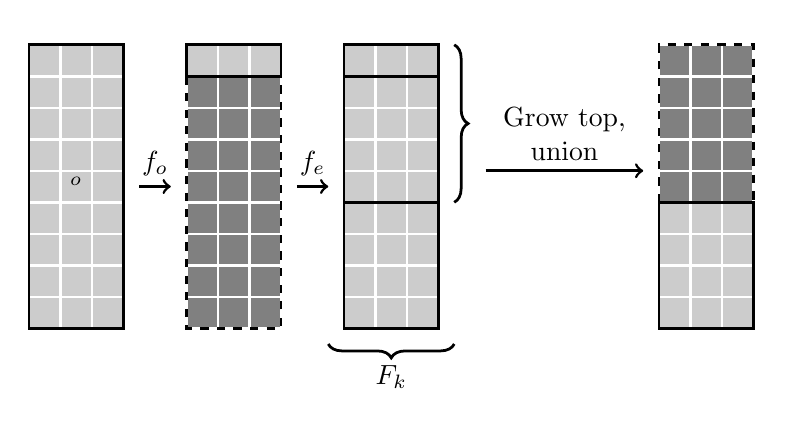
\begin{tikzpicture}[scale=0.4]
      \foreach \x in {0,...,2}{\foreach \y in {0,...,8}{
       \path[fill=white!80!black] (\x,\y) \Square{0.46cm};
      }}
      \draw[l1] (0,0) ++(-.5,-.5) rectangle +(3,9);

      \begin{scope}[shift={(5,0)}]
      \foreach \x in {0,...,2}{
        \foreach \y in {0,...,7}{
          \path[fill=white!50!black] (\x,\y) \Square{0.46cm};}
        \path[fill=white!80!black] (\x,8) \Square{0.46cm};}

      \draw[l1,dashed] (-.5,-.5) ++(0,8) -- ++(0,-8) -- ++(3,0) -- +(0,8);
      \draw[l1] (0,8) ++(-.5,-.5) rectangle +(3,1);
      \end{scope}

      \begin{scope}[shift={(10,0)}]
        \foreach \x in {0,...,2}{\foreach \y in {0,...,8}{
       \path[fill=white!80!black] (\x,\y) \Square{0.46cm};
      }}
      \draw[l1] (0,0) ++(-.5,-.5) rectangle +(3,4);
      \draw[l1] (0,4) ++(-.5,-.5) rectangle +(3,4);
      \draw[l1] (0,8) ++(-.5,-.5) rectangle +(3,1);

      \draw[l1, decorate, decoration={brace, amplitude=5}] (3,9) ++(0,-.5) -- +(0,-5);
      \draw[l1, ->] (4,4.5) -- +(5,0) node [midway, above, text width = 5cm, align=center] {\codefunc{Grow} top, \\union};
      \draw[l1, decorate, decoration={brace, amplitude=5}] (3,0) ++(0,-1) -- +(-4,0) node[midway, below=4pt] {$\m{F}_k$};
      \end{scope}

      \begin{scope}[shift={(20,0)}]
        \foreach \x in {0,...,2}{
        \foreach \y in {0,...,3}{\path[fill=white!80!black] (\x,\y) \Square{0.46cm};}
        \foreach \y in {4,...,8}{\path[fill=white!50!black] (\x,\y) \Square{0.46cm};}}
      \draw[l1] (0,0) ++(-.5,-.5) rectangle +(3,4);
      \draw[l1, dashed] (0,4) ++(-.5,-.5) -- ++(0,5) -- ++(3,0) -- +(0,-5);

      \end{scope}

      \draw[l1, ->] (3,4) -- +(1,0) node[midway, above] {$f_o$};
      \draw[l1, ->] (8,4) -- +(1,0) node[midway, above] {$f_e$};
      \node at (1,4) {$\nset^o$};
    \end{tikzpicture}
  \caption{A fragmentation step $f$ of $\nset^o$, where the fragmentation ratios are not optimal $R_i \neq \frac{1}{3}$. This fragmentation is not possible, as the clusters in $\m{F}_k$ will grow and join in a different path according to the rules of weighted growth.}\label{fig:fragfratio}
\end{figure}

The last unknown parameter for the maximization of $N_{PDC}$ in Equation \eqref{eq:npdc} is $p$, the total number of fragmentation steps. If we assume that in every growth step, not a single non-node vertex is added $N_v = 0$, the full fragmentation of odd node-tree $\pre{0}nset^o$ is just the continuous division of the set in 3 parts per Theorem \ref{lem:fragratio}, which can be calculated easily.
\begin{equation}\label{eq:numfrag}
  p \leq \log_3(\abs{\pre{0}\nset^o})
\end{equation}
In every partial fragmentation set $\m{F}^o_k$, the sum of even node-tree sizes is 
\begin{equation}\label{eq:sumevensetsize}
  \sum_j \left\{ \abs{\pre{k}\nset_j^e} \big| \pre{k}\nset_j^e \in \m{F}^o_k \right\} \leq \frac{2}{3}\abs{\pre{0}\nset^o},
\end{equation}
as $R_1+R_2 = \frac{2}{3}$ per Theorem \ref{the:fragratio} and this value is constant for every fragmentation step is constant per Lemma \ref{lem:equalevensum}. This is an inequality as we have assumed $|\nset| = |\vset|$ and $N_v=0$ in Theorem \ref{the:fragratio}. Filling in equation \eqref{eq:numfrag} and \eqref{eq:sumevensetsize} in \eqref{eq:npdc}, we find that
\begin{align}
% \nonumber % Remove numbering (before each equation)
\nonumber &N_{PDC}  &\leq \sum_{k=1}^{p} \sum_j \left\{ \abs{\pre{k}\nset_j^e} \big| \pre{k}\nset_j^e \in \m{F}^o_k \right\}.  &\\
\nonumber          &&\leq \sum_{k=1}^{\log_3(\abs{\pre{0}\nset^o})} \frac{2}{3}\abs{\pre{0}\nset^o} &\\
                  &&\leq \frac{2}{3}\abs{\pre{0}\nset^o}\log{\abs{\pre{0}\nset^o}} &
\end{align}

Recall from Equation \eqref{eq:limitnsetsize} that the node-tree size is bounded by the lattice size $|\pre{0}\nset^o| \leq N$. The worst-case time complexity of the delay computation is thus bounded by $\m{O}(N\log{N})$. The average-case complexity is even lower as it is almost certain that not all vertices are nodes such that $|\nset| < |\vset|$ and $N_v \neq 0$.

\subsection{Bloom complexity}\label{sec:bloomcomplexity}

To grow a cluster represented by a node-tree $\nset$, a depth-first search is performed on the node-tree to iterate over each boundary list that are stored at the nodes. 
\begin{definition}\label{def:nbloom}
  Let the total number of times nodes are bloomed with \codefunc{Bloom} be $N_{bloom}$.
\end{definition}

Similar to the previous section, we assume a maximum number of nodes on the lattice where, in each cluster $|\nset| = |\vset|$ and $V_v = 0$. For a fragmentation step of $f(\pre{k-1}\nset^o)$ to $\{\pre{k}\nset^o_0, \pre{k}\nset^o_1, \pre{k}\nset^o_2\}$, $N_{bloom}$ is maximized if all three ancestral node-trees are grown. As the growth of every set $\nset$ adds $|\nset|$ to $N_{bloom}$, the total number of bloom can be found similarly to $N_{PDC}$ in Equation \eqref{eq:npdc}. The sum is now on all odd node-tree sizes in all $p$ fragmentation steps $\m{F}_k$: 
\begin{equation}\label{eq:nnode}
  N_{bloom} \leq \sum^{p}_{k=1}\sum_j \left\{ \abs{\pre{k}\nset^o_j} \big| \pre{k}\nset^o_j \in \m{F}_k \right\}
\end{equation}
For a full fragmentation of $\nset$ of size $S_\nset$, the sum of all set sizes in each fragmentation set $\m{F}$ is
\begin{equation}\label{eq:sumsetsfrag}
  \sum_j \left\{ \abs{\pre{k}\nset_j} \big| \pre{k}\nset^o_j \in \m{F}_k \right\} = \abs{\pre{0}\nset^o}.
\end{equation}
By filling in $p$ from \eqref{eq:numfrag}, we find that
\begin{align}
% \nonumber % Remove numbering (before each equation)
  \nonumber & N_{bloom} &\leq \sum^{p}_{k=1}\sum_j \left\{ \abs{\pre{k}\nset^o_j} \big| \pre{k}\nset^o_j \in \m{F}_k \right\} &\\
  \nonumber             &&\leq \sum_{k=1}^{\log_3{\abs{\pre{0}\nset^o}}} \abs{\pre{0}\nset^o} &\\
                        &&\leq \abs{\pre{0}\nset^o}\log_3{\abs{\pre{0}\nset^o}}, &
\end{align}
which again corresponds to a worst-case time complexity that is bounded by $\m{O}(N\log{N})$.

\section{Compatibility}\label{sec:ufbbcompatibility}

In this section, we shortly describe how to alter the Union-Find Balanced-Bloom decoder of Algorithm \ref{algo:ufbb} to be compatible with surfaces with boundaries such as the planar code (Section \ref{sec:surface_planar}), and erasure errors. 

\subsection{Surfaces with boundaries}\label{sec:ufbbbound}
We introduced the concept of \emph{open vertices} $\vset_\omega$ for surfaces with boundaries that, in contrast to normal vertices, are not equivalent to stabilizers, measurements, or ancillary qubits (Section \ref{sec:surface_planar}). During the formation of the spanning forest $\m{T}_\m{R}$ of a cluster, we must make sure that $\m{T}_\m{R}$ does not contain more than one element of the set of boundary vertices $\vset_\omega$, as multiple elements of $\vset_\omega$ is equivalent to a cycle (Section \ref{sec:peelingbound}).
\begin{definition}\label{def:boundarynode}
  Let a boundary-node $b$ denote a node that is seeded in an open-vertex $v \in \vset_\omega$. 
\end{definition}
The addition of boundaries requires a new type of node element, the \emph{boundary node} $n$, that is exclusive to boundary vertices of $\vset_\omega$, and are initiated on a boundary vertex if a cluster grows into the boundary. Recall from Section \ref{sec:peelingbound} that there can be only one boundary vertex in $\vset$. For this reason, there can be only one boundary node in $\nset$. As a result, a boundary node will always be a trailing node in $\nset$ with no children, and will never be the root node. However, the always-trailing boundary node always has parity 1, as a matching with the boundary is equally valid as a matching with another syndrome. The addition of boundary nodes just requires a small alteration to Algorithm \ref{algo:calcparity}.
\begin{algorithm}[htbp]
  \SetKwFunction{cp}{Calcparity}
  \SetKwFunction{summation}{Sum}
  \KwData{Node $n$}
  \KwResult{Calculated parities for $n$ and all its descendent nodes}
  \BlankLine
  parity $=$ \summation{$[1 - $ \cp{$n_\gamma$} $\forall$ children $n_\gamma$ of $n]$} $\bmod 2$\;
  \uIf(syndrome-node){$n \equiv s$}{
      $n.p =$ parity}
  \uElseIf(linking-node){$n \equiv l$}{
      $n.p= 1-$ parity}
  \ElseIf(boundary-node){$n \equiv b$}{
    $n.p= 1$}
  \KwRet{$n.p$}
  \caption{\codefunc{Calcparity} for surfaces with boundaries}\label{algo:calcparitybound}
\end{algorithm}


For a surface containing $N$ qubits, the number of boundary elements scales with $\sqrt{N}$. The number of node elements is thus bounded by $N + \sqrt{N}$. Therefore, the added complexity due to the boundary elements will not exceed some linear factor and remains the same as previously computed.

\subsection{Erasure noise}\label{sec:ufbberasure}

The inspiration for the Union-Find decoder is the Peeling decoder (Section \ref{sec:peelingdecoder}), that only accounted for \emph{erasure} errors. As the Union-Find Balanced-Bloom decoder is a modification of the Union-Find decoder, we naturally need to make sure that it can also solve erasure errors.

To account for these erasures, we must construct the node-trees for these initial erasure clusters. We can easily check that for an erasure-cluster, the potential matching for every neighboring vertex is different. Therefore, every vertex in the cluster is a node in $\nset$, where each syndrome-vertex is a syndrome-node $\sigma$, and every other vertex is a linking-node $l$. Note that if the erasure is connected to the boundary, we need to make sure that only a single edge is connected to the boundary. The single boundary vertex in the cluster is then naturally a boundary node $b$. After constructing these initial clusters and node-trees, we can proceed to the Union-Find Balanced Bloom decoder.  

\section{Performance}

We benchmark the performance of the Union-Find Balanced-Bloom decoder of Algorithm \ref{algo:ufbb} using our application in Python3 (see Appendix \ref{ap:oopsurfacecode}). This is done by Monte Carlo simulations of decoding on a simulated lattice and to fit for the code threshold, described in Section \ref{sec:simthres}. For the independent noise model (Definition \ref{def:independent}), we simulate on lattice sizes $L_{small}=[8, 16, 24, 32, 40, 48, 56, 64]$ with a minimum of $96.000$ samples and on $L_{big}=[72, 80, 88, 96]$ with a minimum of $28.800$ samples. For the phenomenological noise model (Definition \ref{def:pheno}), we simulate on lattice sizes $L_{small}=[8,12,16,20,24]$ with a minimum of $105.600$ samples and on lattice sizes $L_{big}=[28, 32, 36, 40, 44]$ with $13.200$ samples. The code thresholds for the toric and planar codes with independent and phenomenological noise are listed in Table \ref{tab:ufbb}, which also includes thresholds of the Minimum Weight Perfect Matching (MWPM) decoder (Table \ref{tab:mwpm}) and the Dynamic-forest Bucket Union-Find (DBUF) decoder (Table \ref{tab:uftable}) for comparison.
\begin{table}[htbp]
  \centering
  \begin{tabularx}{\textwidth}{ | L{.7} | R{0.7} || C{1.7} | C{.6} | C{1.7} | C{.6} | }
    \hline
    \multicolumn{2}{|c|}{\multirow{2}{*}{}} & \multicolumn{2}{c|}{Independent noise}& \multicolumn{2}{c|}{Phenomenological noise} \\
    \cline{3-6}
    \multicolumn{2}{|c|}{}    & $p_{th}$ & $k_{th}$ & $p_{th}$ & $k_{th}$ \\
    \hhline{|--::=:=:=:=|}
    \multirow{4}{*}{Toric}  &\gc MWPM &\gc $0.10349 \pm 0.00004$ &\gc $0.7158$ &\gc $0.02965 \pm 0.00003$ &\gc $0.9024$ \\
                            \cline{2-6}
                            &\gc DBUF &\gc $0.10014 \pm 0.00003$ &\gc $0.7271$ &\gc $0.02685 \pm 0.00001$ &\gc $0.9208$ \\
                            \cline{2-6}
                            & $L_{small}$ & $0.10229 \pm 0.00007$ & $0.7312$ & $0.02846 \pm 0.00003$ & $0.9165$ \\
                            \cline{2-6}
                            & $L_{big}$ & $0.1007 \pm 0.0001$ & $0.7690 $ & $0.0278 \pm 0.0001$ & $0.943$ \\ 
    \hhline{|=:=::=:=:=:=|}
    \multirow{3}{*}{Planar} &\gc MWPM  &\gc $0.10292 \pm 0.00005$ &\gc $0.8478$ &\gc $0.02928 \pm 0.00003$ &\gc $0.928$ \\
                            \cline{2-6}
                            &\gc DBUF &\gc $0.09974 \pm 0.00004$ &\gc $0.8480$ &\gc $0.02660 \pm 0.00001$ &\gc $0.9322$\\
                            \cline{2-6}
                            & $L_{small}$ & $0.0993 \pm 0.0001$ & $0.8689$ & $0.02711 \pm 0.00006$ & $0.9480$ \\
                            \cline{2-6}
                            & $L_{big}$ & $0.0961 \pm 0.0004$ & $0.905$ &$0.02455 \pm 0.0004$ & $0.982$ \\
                             
    \hline
  \end{tabularx}
  \caption{Error thresholds for the Union-Find Balanced-Bloom decoder (Algorithm \ref{algo:bbgrow}) on both the toric and planar lattices with independent and phenomenological noise. The error thresholds for the Minimum-Weight Perfect Matching decoder of Table \ref{tab:mwpm} and from Dynamic-forest Bucket Union-Find decoder (Algorithm \ref{algo:dbuf}) of Table \ref{tab:uftable} have been added as a comparison. The results of the Monte Carlo simulations for the $L_{small}$ range of lattice sizes used to calculate the thresholds are included in Figure \ref{fig:threshold_ufbbsmall}, and for the $L_{big}$ range of lattice sizes are included in Figure \ref{fig:threshold_ufbbbig}.}\label{tab:ufbb}
\end{table}

\subsection{Threshold}

We had initially simulated for the decoding success rates for the range of lattices in $L_{small}$, which is the same range used when benchmarking the various implementations of the Union-Find decoder in Section \ref{sec:ufperformance}. For $L_{small}$, we find that except for the environment of planar code with independent noise, the thresholds of the Union-Find Balanced-Bloom decoder are increased from the DBUF thresholds, and moves close to the thresholds of the MWPM decoder. We also observe an increase in decoding success rate at the threshold $k_{th}$ from DBUF, which is also the case for the environment of planar code with independent noise. For the range of lattices in $L_{big}$ (Figure \ref{fig:threshold_ufbbbig}), the threshold of the Union-Find Balanced-Bloom decoder decreases to below DBUF thresholds. This does not necessarily mean that it performs worse, as $k_{th}$ is still above DBUF's values, but does raise questions on the scalability of the Union-Find Balanced-Bloom decoder. In fact, if we look closely at the values of $k_C$ (Figure \ref{fig:thres_ufbb_toric_2d_data}), we find that the fit does not accurately represent the underlying data points, which is different behavior from the MWPM and DBUF decoders. The threshold and $k_C$ of the Union-Find Balanced-Bloom decoder may not be accurate for comparison. 

For this reason, we have applied a \emph{sequential fit} to the data acquired in the Monte Carlo simulations of lattices of $L = L_{small} \cup L_{big}$. In the sequential fit, we iterate stepwise in the ordered list of lattice sizes $L$ and fit for the data of $L_i, L_{i+1}$ for $i \in |L|-1$ iterations. The fit thus returns an error threshold in the range of the chosen lattices sizes. The range of thresholds $p_{th}(L_i, L_{i+1})$ for the environment of toric code with independent noise is plotted in Figure \ref{fig:thres_ufbb_toric_2d_seq}. We see that the sequential fits follow a trend where the increase in the input lattice sizes results in a decrease in $p_{th}$ but increase in $k_{th}$. The range of thresholds coordinates $(p_{th}, k_{th})$ is plotted in Figure \ref{fig:thres_ufbb_toric_2d_comp}, together with the data acquired from the simulations for the performance of the MWPM decoder and the DBUF decoder. Similar figures for the planar code with independent noise, both the toric and planar codes with phenomenological noise are included in Figures \ref{fig:thres_ufbb_planar_2d}, \ref{fig:thres_ufbb_toric_3d}, and \ref{fig:thres_ufbb_planar_3d}. 

We ascribe the degradation of the threshold error rate to the \emph{parity inversion} effect, explained in Section \ref{sec:eqstate}. Recall from Lemma \ref{lem:parityinversion} that the number of iterations waited before a union $I_t$ is proportional to the number of iterations required to reach the balanced-bloom state (Definition \ref{def:balancedbloom}) $M_{t+1}$, where $(I:M)$ is the equilibrium state of Definition \ref{def:eqstate}. By setting the equilibrium factor to $k_{eq}=\frac{1}{2}$, the equilibrium state is occupied half on average. The degradation is caused by the proportionality of the number of parity inversions and consequently equilibrium-state parameter $M$ to the lattice size. As the lattice size increases, the equilibrium state is still occupied half on average, but the absolute difference in $M-I$ increases. It is thus increasingly more unlikely that the balanced-bloom state is reached. 

Overall, the Union-Find Balanced-Bloom decoder has an increased error threshold $p_{th}$ from the threshold of the Union-Find decoder for small lattice sizes and is comparable to the threshold values of the Minimum-Weight Perfect Matching decoder. The error threshold decreases for larger lattice sizes, but the Union-Find Balanced-Bloom decoder still has an increased performance, which is now defined by an increased decoding success rate at the threshold $k_{th}$. The improvement across all lattice sizes is most apparent when comparing the range of threshold coordinates in $(p_X, k_C)$ space, where the coordinates now occupy a range that is not possible with the Union-Find decoder. 

\begin{figure}[htbp]
  \centering
  \begin{subfigure}[b]{0.49\textwidth}
    \begin{adjustbox}{Clip=0 1em 0 0}
      %% Creator: Matplotlib, PGF backend
%%
%% To include the figure in your LaTeX document, write
%%   \input{<filename>.pgf}
%%
%% Make sure the required packages are loaded in your preamble
%%   \usepackage{pgf}
%%
%% Figures using additional raster images can only be included by \input if
%% they are in the same directory as the main LaTeX file. For loading figures
%% from other directories you can use the `import` package
%%   \usepackage{import}
%% and then include the figures with
%%   \import{<path to file>}{<filename>.pgf}
%%
%% Matplotlib used the following preamble
%%   \usepackage[utf8x]{inputenc}
%%   \usepackage[T1]{fontenc}
%%
\begingroup%
\makeatletter%
\begin{pgfpicture}%
\pgfpathrectangle{\pgfpointorigin}{\pgfqpoint{3.000000in}{3.000000in}}%
\pgfusepath{use as bounding box, clip}%
\begin{pgfscope}%
\pgfsetbuttcap%
\pgfsetmiterjoin%
\definecolor{currentfill}{rgb}{1.000000,1.000000,1.000000}%
\pgfsetfillcolor{currentfill}%
\pgfsetlinewidth{0.000000pt}%
\definecolor{currentstroke}{rgb}{1.000000,1.000000,1.000000}%
\pgfsetstrokecolor{currentstroke}%
\pgfsetdash{}{0pt}%
\pgfpathmoveto{\pgfqpoint{0.000000in}{0.000000in}}%
\pgfpathlineto{\pgfqpoint{3.000000in}{0.000000in}}%
\pgfpathlineto{\pgfqpoint{3.000000in}{3.000000in}}%
\pgfpathlineto{\pgfqpoint{0.000000in}{3.000000in}}%
\pgfpathclose%
\pgfusepath{fill}%
\end{pgfscope}%
\begin{pgfscope}%
\pgfsetbuttcap%
\pgfsetmiterjoin%
\definecolor{currentfill}{rgb}{1.000000,1.000000,1.000000}%
\pgfsetfillcolor{currentfill}%
\pgfsetlinewidth{0.000000pt}%
\definecolor{currentstroke}{rgb}{0.000000,0.000000,0.000000}%
\pgfsetstrokecolor{currentstroke}%
\pgfsetstrokeopacity{0.000000}%
\pgfsetdash{}{0pt}%
\pgfpathmoveto{\pgfqpoint{0.694341in}{0.523557in}}%
\pgfpathlineto{\pgfqpoint{2.821228in}{0.523557in}}%
\pgfpathlineto{\pgfqpoint{2.821228in}{2.850000in}}%
\pgfpathlineto{\pgfqpoint{0.694341in}{2.850000in}}%
\pgfpathclose%
\pgfusepath{fill}%
\end{pgfscope}%
\begin{pgfscope}%
\pgfpathrectangle{\pgfqpoint{0.694341in}{0.523557in}}{\pgfqpoint{2.126887in}{2.326443in}}%
\pgfusepath{clip}%
\pgfsetbuttcap%
\pgfsetroundjoin%
\pgfsetlinewidth{0.501875pt}%
\definecolor{currentstroke}{rgb}{0.690196,0.690196,0.690196}%
\pgfsetstrokecolor{currentstroke}%
\pgfsetdash{{0.500000pt}{0.825000pt}}{0.000000pt}%
\pgfpathmoveto{\pgfqpoint{0.791018in}{0.523557in}}%
\pgfpathlineto{\pgfqpoint{0.791018in}{2.850000in}}%
\pgfusepath{stroke}%
\end{pgfscope}%
\begin{pgfscope}%
\pgfsetbuttcap%
\pgfsetroundjoin%
\definecolor{currentfill}{rgb}{0.000000,0.000000,0.000000}%
\pgfsetfillcolor{currentfill}%
\pgfsetlinewidth{0.803000pt}%
\definecolor{currentstroke}{rgb}{0.000000,0.000000,0.000000}%
\pgfsetstrokecolor{currentstroke}%
\pgfsetdash{}{0pt}%
\pgfsys@defobject{currentmarker}{\pgfqpoint{0.000000in}{-0.048611in}}{\pgfqpoint{0.000000in}{0.000000in}}{%
\pgfpathmoveto{\pgfqpoint{0.000000in}{0.000000in}}%
\pgfpathlineto{\pgfqpoint{0.000000in}{-0.048611in}}%
\pgfusepath{stroke,fill}%
}%
\begin{pgfscope}%
\pgfsys@transformshift{0.791018in}{0.523557in}%
\pgfsys@useobject{currentmarker}{}%
\end{pgfscope}%
\end{pgfscope}%
\begin{pgfscope}%
\definecolor{textcolor}{rgb}{0.000000,0.000000,0.000000}%
\pgfsetstrokecolor{textcolor}%
\pgfsetfillcolor{textcolor}%
\pgftext[x=0.791018in,y=0.426335in,,top]{\color{textcolor}\rmfamily\fontsize{8.000000}{9.600000}\selectfont \(\displaystyle 0.099\)}%
\end{pgfscope}%
\begin{pgfscope}%
\pgfpathrectangle{\pgfqpoint{0.694341in}{0.523557in}}{\pgfqpoint{2.126887in}{2.326443in}}%
\pgfusepath{clip}%
\pgfsetbuttcap%
\pgfsetroundjoin%
\pgfsetlinewidth{0.501875pt}%
\definecolor{currentstroke}{rgb}{0.690196,0.690196,0.690196}%
\pgfsetstrokecolor{currentstroke}%
\pgfsetdash{{0.500000pt}{0.825000pt}}{0.000000pt}%
\pgfpathmoveto{\pgfqpoint{1.177724in}{0.523557in}}%
\pgfpathlineto{\pgfqpoint{1.177724in}{2.850000in}}%
\pgfusepath{stroke}%
\end{pgfscope}%
\begin{pgfscope}%
\pgfsetbuttcap%
\pgfsetroundjoin%
\definecolor{currentfill}{rgb}{0.000000,0.000000,0.000000}%
\pgfsetfillcolor{currentfill}%
\pgfsetlinewidth{0.803000pt}%
\definecolor{currentstroke}{rgb}{0.000000,0.000000,0.000000}%
\pgfsetstrokecolor{currentstroke}%
\pgfsetdash{}{0pt}%
\pgfsys@defobject{currentmarker}{\pgfqpoint{0.000000in}{-0.048611in}}{\pgfqpoint{0.000000in}{0.000000in}}{%
\pgfpathmoveto{\pgfqpoint{0.000000in}{0.000000in}}%
\pgfpathlineto{\pgfqpoint{0.000000in}{-0.048611in}}%
\pgfusepath{stroke,fill}%
}%
\begin{pgfscope}%
\pgfsys@transformshift{1.177724in}{0.523557in}%
\pgfsys@useobject{currentmarker}{}%
\end{pgfscope}%
\end{pgfscope}%
\begin{pgfscope}%
\definecolor{textcolor}{rgb}{0.000000,0.000000,0.000000}%
\pgfsetstrokecolor{textcolor}%
\pgfsetfillcolor{textcolor}%
\pgftext[x=1.177724in,y=0.426335in,,top]{\color{textcolor}\rmfamily\fontsize{8.000000}{9.600000}\selectfont \(\displaystyle 0.100\)}%
\end{pgfscope}%
\begin{pgfscope}%
\pgfpathrectangle{\pgfqpoint{0.694341in}{0.523557in}}{\pgfqpoint{2.126887in}{2.326443in}}%
\pgfusepath{clip}%
\pgfsetbuttcap%
\pgfsetroundjoin%
\pgfsetlinewidth{0.501875pt}%
\definecolor{currentstroke}{rgb}{0.690196,0.690196,0.690196}%
\pgfsetstrokecolor{currentstroke}%
\pgfsetdash{{0.500000pt}{0.825000pt}}{0.000000pt}%
\pgfpathmoveto{\pgfqpoint{1.564431in}{0.523557in}}%
\pgfpathlineto{\pgfqpoint{1.564431in}{2.850000in}}%
\pgfusepath{stroke}%
\end{pgfscope}%
\begin{pgfscope}%
\pgfsetbuttcap%
\pgfsetroundjoin%
\definecolor{currentfill}{rgb}{0.000000,0.000000,0.000000}%
\pgfsetfillcolor{currentfill}%
\pgfsetlinewidth{0.803000pt}%
\definecolor{currentstroke}{rgb}{0.000000,0.000000,0.000000}%
\pgfsetstrokecolor{currentstroke}%
\pgfsetdash{}{0pt}%
\pgfsys@defobject{currentmarker}{\pgfqpoint{0.000000in}{-0.048611in}}{\pgfqpoint{0.000000in}{0.000000in}}{%
\pgfpathmoveto{\pgfqpoint{0.000000in}{0.000000in}}%
\pgfpathlineto{\pgfqpoint{0.000000in}{-0.048611in}}%
\pgfusepath{stroke,fill}%
}%
\begin{pgfscope}%
\pgfsys@transformshift{1.564431in}{0.523557in}%
\pgfsys@useobject{currentmarker}{}%
\end{pgfscope}%
\end{pgfscope}%
\begin{pgfscope}%
\definecolor{textcolor}{rgb}{0.000000,0.000000,0.000000}%
\pgfsetstrokecolor{textcolor}%
\pgfsetfillcolor{textcolor}%
\pgftext[x=1.564431in,y=0.426335in,,top]{\color{textcolor}\rmfamily\fontsize{8.000000}{9.600000}\selectfont \(\displaystyle 0.101\)}%
\end{pgfscope}%
\begin{pgfscope}%
\pgfpathrectangle{\pgfqpoint{0.694341in}{0.523557in}}{\pgfqpoint{2.126887in}{2.326443in}}%
\pgfusepath{clip}%
\pgfsetbuttcap%
\pgfsetroundjoin%
\pgfsetlinewidth{0.501875pt}%
\definecolor{currentstroke}{rgb}{0.690196,0.690196,0.690196}%
\pgfsetstrokecolor{currentstroke}%
\pgfsetdash{{0.500000pt}{0.825000pt}}{0.000000pt}%
\pgfpathmoveto{\pgfqpoint{1.951138in}{0.523557in}}%
\pgfpathlineto{\pgfqpoint{1.951138in}{2.850000in}}%
\pgfusepath{stroke}%
\end{pgfscope}%
\begin{pgfscope}%
\pgfsetbuttcap%
\pgfsetroundjoin%
\definecolor{currentfill}{rgb}{0.000000,0.000000,0.000000}%
\pgfsetfillcolor{currentfill}%
\pgfsetlinewidth{0.803000pt}%
\definecolor{currentstroke}{rgb}{0.000000,0.000000,0.000000}%
\pgfsetstrokecolor{currentstroke}%
\pgfsetdash{}{0pt}%
\pgfsys@defobject{currentmarker}{\pgfqpoint{0.000000in}{-0.048611in}}{\pgfqpoint{0.000000in}{0.000000in}}{%
\pgfpathmoveto{\pgfqpoint{0.000000in}{0.000000in}}%
\pgfpathlineto{\pgfqpoint{0.000000in}{-0.048611in}}%
\pgfusepath{stroke,fill}%
}%
\begin{pgfscope}%
\pgfsys@transformshift{1.951138in}{0.523557in}%
\pgfsys@useobject{currentmarker}{}%
\end{pgfscope}%
\end{pgfscope}%
\begin{pgfscope}%
\definecolor{textcolor}{rgb}{0.000000,0.000000,0.000000}%
\pgfsetstrokecolor{textcolor}%
\pgfsetfillcolor{textcolor}%
\pgftext[x=1.951138in,y=0.426335in,,top]{\color{textcolor}\rmfamily\fontsize{8.000000}{9.600000}\selectfont \(\displaystyle 0.102\)}%
\end{pgfscope}%
\begin{pgfscope}%
\pgfpathrectangle{\pgfqpoint{0.694341in}{0.523557in}}{\pgfqpoint{2.126887in}{2.326443in}}%
\pgfusepath{clip}%
\pgfsetbuttcap%
\pgfsetroundjoin%
\pgfsetlinewidth{0.501875pt}%
\definecolor{currentstroke}{rgb}{0.690196,0.690196,0.690196}%
\pgfsetstrokecolor{currentstroke}%
\pgfsetdash{{0.500000pt}{0.825000pt}}{0.000000pt}%
\pgfpathmoveto{\pgfqpoint{2.337844in}{0.523557in}}%
\pgfpathlineto{\pgfqpoint{2.337844in}{2.850000in}}%
\pgfusepath{stroke}%
\end{pgfscope}%
\begin{pgfscope}%
\pgfsetbuttcap%
\pgfsetroundjoin%
\definecolor{currentfill}{rgb}{0.000000,0.000000,0.000000}%
\pgfsetfillcolor{currentfill}%
\pgfsetlinewidth{0.803000pt}%
\definecolor{currentstroke}{rgb}{0.000000,0.000000,0.000000}%
\pgfsetstrokecolor{currentstroke}%
\pgfsetdash{}{0pt}%
\pgfsys@defobject{currentmarker}{\pgfqpoint{0.000000in}{-0.048611in}}{\pgfqpoint{0.000000in}{0.000000in}}{%
\pgfpathmoveto{\pgfqpoint{0.000000in}{0.000000in}}%
\pgfpathlineto{\pgfqpoint{0.000000in}{-0.048611in}}%
\pgfusepath{stroke,fill}%
}%
\begin{pgfscope}%
\pgfsys@transformshift{2.337844in}{0.523557in}%
\pgfsys@useobject{currentmarker}{}%
\end{pgfscope}%
\end{pgfscope}%
\begin{pgfscope}%
\definecolor{textcolor}{rgb}{0.000000,0.000000,0.000000}%
\pgfsetstrokecolor{textcolor}%
\pgfsetfillcolor{textcolor}%
\pgftext[x=2.337844in,y=0.426335in,,top]{\color{textcolor}\rmfamily\fontsize{8.000000}{9.600000}\selectfont \(\displaystyle 0.103\)}%
\end{pgfscope}%
\begin{pgfscope}%
\pgfpathrectangle{\pgfqpoint{0.694341in}{0.523557in}}{\pgfqpoint{2.126887in}{2.326443in}}%
\pgfusepath{clip}%
\pgfsetbuttcap%
\pgfsetroundjoin%
\pgfsetlinewidth{0.501875pt}%
\definecolor{currentstroke}{rgb}{0.690196,0.690196,0.690196}%
\pgfsetstrokecolor{currentstroke}%
\pgfsetdash{{0.500000pt}{0.825000pt}}{0.000000pt}%
\pgfpathmoveto{\pgfqpoint{2.724551in}{0.523557in}}%
\pgfpathlineto{\pgfqpoint{2.724551in}{2.850000in}}%
\pgfusepath{stroke}%
\end{pgfscope}%
\begin{pgfscope}%
\pgfsetbuttcap%
\pgfsetroundjoin%
\definecolor{currentfill}{rgb}{0.000000,0.000000,0.000000}%
\pgfsetfillcolor{currentfill}%
\pgfsetlinewidth{0.803000pt}%
\definecolor{currentstroke}{rgb}{0.000000,0.000000,0.000000}%
\pgfsetstrokecolor{currentstroke}%
\pgfsetdash{}{0pt}%
\pgfsys@defobject{currentmarker}{\pgfqpoint{0.000000in}{-0.048611in}}{\pgfqpoint{0.000000in}{0.000000in}}{%
\pgfpathmoveto{\pgfqpoint{0.000000in}{0.000000in}}%
\pgfpathlineto{\pgfqpoint{0.000000in}{-0.048611in}}%
\pgfusepath{stroke,fill}%
}%
\begin{pgfscope}%
\pgfsys@transformshift{2.724551in}{0.523557in}%
\pgfsys@useobject{currentmarker}{}%
\end{pgfscope}%
\end{pgfscope}%
\begin{pgfscope}%
\definecolor{textcolor}{rgb}{0.000000,0.000000,0.000000}%
\pgfsetstrokecolor{textcolor}%
\pgfsetfillcolor{textcolor}%
\pgftext[x=2.724551in,y=0.426335in,,top]{\color{textcolor}\rmfamily\fontsize{8.000000}{9.600000}\selectfont \(\displaystyle 0.104\)}%
\end{pgfscope}%
\begin{pgfscope}%
\definecolor{textcolor}{rgb}{0.000000,0.000000,0.000000}%
\pgfsetstrokecolor{textcolor}%
\pgfsetfillcolor{textcolor}%
\pgftext[x=1.757784in,y=0.272655in,,top]{\color{textcolor}\rmfamily\fontsize{10.000000}{12.000000}\selectfont  \(\displaystyle  p_X \)}%
\end{pgfscope}%
\begin{pgfscope}%
\pgfpathrectangle{\pgfqpoint{0.694341in}{0.523557in}}{\pgfqpoint{2.126887in}{2.326443in}}%
\pgfusepath{clip}%
\pgfsetbuttcap%
\pgfsetroundjoin%
\pgfsetlinewidth{0.501875pt}%
\definecolor{currentstroke}{rgb}{0.690196,0.690196,0.690196}%
\pgfsetstrokecolor{currentstroke}%
\pgfsetdash{{0.500000pt}{0.825000pt}}{0.000000pt}%
\pgfpathmoveto{\pgfqpoint{0.694341in}{0.538993in}}%
\pgfpathlineto{\pgfqpoint{2.821228in}{0.538993in}}%
\pgfusepath{stroke}%
\end{pgfscope}%
\begin{pgfscope}%
\pgfsetbuttcap%
\pgfsetroundjoin%
\definecolor{currentfill}{rgb}{0.000000,0.000000,0.000000}%
\pgfsetfillcolor{currentfill}%
\pgfsetlinewidth{0.803000pt}%
\definecolor{currentstroke}{rgb}{0.000000,0.000000,0.000000}%
\pgfsetstrokecolor{currentstroke}%
\pgfsetdash{}{0pt}%
\pgfsys@defobject{currentmarker}{\pgfqpoint{-0.048611in}{0.000000in}}{\pgfqpoint{0.000000in}{0.000000in}}{%
\pgfpathmoveto{\pgfqpoint{0.000000in}{0.000000in}}%
\pgfpathlineto{\pgfqpoint{-0.048611in}{0.000000in}}%
\pgfusepath{stroke,fill}%
}%
\begin{pgfscope}%
\pgfsys@transformshift{0.694341in}{0.538993in}%
\pgfsys@useobject{currentmarker}{}%
\end{pgfscope}%
\end{pgfscope}%
\begin{pgfscope}%
\definecolor{textcolor}{rgb}{0.000000,0.000000,0.000000}%
\pgfsetstrokecolor{textcolor}%
\pgfsetfillcolor{textcolor}%
\pgftext[x=0.328211in,y=0.500731in,left,base]{\color{textcolor}\rmfamily\fontsize{8.000000}{9.600000}\selectfont \(\displaystyle 0.625\)}%
\end{pgfscope}%
\begin{pgfscope}%
\pgfpathrectangle{\pgfqpoint{0.694341in}{0.523557in}}{\pgfqpoint{2.126887in}{2.326443in}}%
\pgfusepath{clip}%
\pgfsetbuttcap%
\pgfsetroundjoin%
\pgfsetlinewidth{0.501875pt}%
\definecolor{currentstroke}{rgb}{0.690196,0.690196,0.690196}%
\pgfsetstrokecolor{currentstroke}%
\pgfsetdash{{0.500000pt}{0.825000pt}}{0.000000pt}%
\pgfpathmoveto{\pgfqpoint{0.694341in}{0.811061in}}%
\pgfpathlineto{\pgfqpoint{2.821228in}{0.811061in}}%
\pgfusepath{stroke}%
\end{pgfscope}%
\begin{pgfscope}%
\pgfsetbuttcap%
\pgfsetroundjoin%
\definecolor{currentfill}{rgb}{0.000000,0.000000,0.000000}%
\pgfsetfillcolor{currentfill}%
\pgfsetlinewidth{0.803000pt}%
\definecolor{currentstroke}{rgb}{0.000000,0.000000,0.000000}%
\pgfsetstrokecolor{currentstroke}%
\pgfsetdash{}{0pt}%
\pgfsys@defobject{currentmarker}{\pgfqpoint{-0.048611in}{0.000000in}}{\pgfqpoint{0.000000in}{0.000000in}}{%
\pgfpathmoveto{\pgfqpoint{0.000000in}{0.000000in}}%
\pgfpathlineto{\pgfqpoint{-0.048611in}{0.000000in}}%
\pgfusepath{stroke,fill}%
}%
\begin{pgfscope}%
\pgfsys@transformshift{0.694341in}{0.811061in}%
\pgfsys@useobject{currentmarker}{}%
\end{pgfscope}%
\end{pgfscope}%
\begin{pgfscope}%
\definecolor{textcolor}{rgb}{0.000000,0.000000,0.000000}%
\pgfsetstrokecolor{textcolor}%
\pgfsetfillcolor{textcolor}%
\pgftext[x=0.328211in,y=0.772799in,left,base]{\color{textcolor}\rmfamily\fontsize{8.000000}{9.600000}\selectfont \(\displaystyle 0.650\)}%
\end{pgfscope}%
\begin{pgfscope}%
\pgfpathrectangle{\pgfqpoint{0.694341in}{0.523557in}}{\pgfqpoint{2.126887in}{2.326443in}}%
\pgfusepath{clip}%
\pgfsetbuttcap%
\pgfsetroundjoin%
\pgfsetlinewidth{0.501875pt}%
\definecolor{currentstroke}{rgb}{0.690196,0.690196,0.690196}%
\pgfsetstrokecolor{currentstroke}%
\pgfsetdash{{0.500000pt}{0.825000pt}}{0.000000pt}%
\pgfpathmoveto{\pgfqpoint{0.694341in}{1.083129in}}%
\pgfpathlineto{\pgfqpoint{2.821228in}{1.083129in}}%
\pgfusepath{stroke}%
\end{pgfscope}%
\begin{pgfscope}%
\pgfsetbuttcap%
\pgfsetroundjoin%
\definecolor{currentfill}{rgb}{0.000000,0.000000,0.000000}%
\pgfsetfillcolor{currentfill}%
\pgfsetlinewidth{0.803000pt}%
\definecolor{currentstroke}{rgb}{0.000000,0.000000,0.000000}%
\pgfsetstrokecolor{currentstroke}%
\pgfsetdash{}{0pt}%
\pgfsys@defobject{currentmarker}{\pgfqpoint{-0.048611in}{0.000000in}}{\pgfqpoint{0.000000in}{0.000000in}}{%
\pgfpathmoveto{\pgfqpoint{0.000000in}{0.000000in}}%
\pgfpathlineto{\pgfqpoint{-0.048611in}{0.000000in}}%
\pgfusepath{stroke,fill}%
}%
\begin{pgfscope}%
\pgfsys@transformshift{0.694341in}{1.083129in}%
\pgfsys@useobject{currentmarker}{}%
\end{pgfscope}%
\end{pgfscope}%
\begin{pgfscope}%
\definecolor{textcolor}{rgb}{0.000000,0.000000,0.000000}%
\pgfsetstrokecolor{textcolor}%
\pgfsetfillcolor{textcolor}%
\pgftext[x=0.328211in,y=1.044866in,left,base]{\color{textcolor}\rmfamily\fontsize{8.000000}{9.600000}\selectfont \(\displaystyle 0.675\)}%
\end{pgfscope}%
\begin{pgfscope}%
\pgfpathrectangle{\pgfqpoint{0.694341in}{0.523557in}}{\pgfqpoint{2.126887in}{2.326443in}}%
\pgfusepath{clip}%
\pgfsetbuttcap%
\pgfsetroundjoin%
\pgfsetlinewidth{0.501875pt}%
\definecolor{currentstroke}{rgb}{0.690196,0.690196,0.690196}%
\pgfsetstrokecolor{currentstroke}%
\pgfsetdash{{0.500000pt}{0.825000pt}}{0.000000pt}%
\pgfpathmoveto{\pgfqpoint{0.694341in}{1.355196in}}%
\pgfpathlineto{\pgfqpoint{2.821228in}{1.355196in}}%
\pgfusepath{stroke}%
\end{pgfscope}%
\begin{pgfscope}%
\pgfsetbuttcap%
\pgfsetroundjoin%
\definecolor{currentfill}{rgb}{0.000000,0.000000,0.000000}%
\pgfsetfillcolor{currentfill}%
\pgfsetlinewidth{0.803000pt}%
\definecolor{currentstroke}{rgb}{0.000000,0.000000,0.000000}%
\pgfsetstrokecolor{currentstroke}%
\pgfsetdash{}{0pt}%
\pgfsys@defobject{currentmarker}{\pgfqpoint{-0.048611in}{0.000000in}}{\pgfqpoint{0.000000in}{0.000000in}}{%
\pgfpathmoveto{\pgfqpoint{0.000000in}{0.000000in}}%
\pgfpathlineto{\pgfqpoint{-0.048611in}{0.000000in}}%
\pgfusepath{stroke,fill}%
}%
\begin{pgfscope}%
\pgfsys@transformshift{0.694341in}{1.355196in}%
\pgfsys@useobject{currentmarker}{}%
\end{pgfscope}%
\end{pgfscope}%
\begin{pgfscope}%
\definecolor{textcolor}{rgb}{0.000000,0.000000,0.000000}%
\pgfsetstrokecolor{textcolor}%
\pgfsetfillcolor{textcolor}%
\pgftext[x=0.328211in,y=1.316934in,left,base]{\color{textcolor}\rmfamily\fontsize{8.000000}{9.600000}\selectfont \(\displaystyle 0.700\)}%
\end{pgfscope}%
\begin{pgfscope}%
\pgfpathrectangle{\pgfqpoint{0.694341in}{0.523557in}}{\pgfqpoint{2.126887in}{2.326443in}}%
\pgfusepath{clip}%
\pgfsetbuttcap%
\pgfsetroundjoin%
\pgfsetlinewidth{0.501875pt}%
\definecolor{currentstroke}{rgb}{0.690196,0.690196,0.690196}%
\pgfsetstrokecolor{currentstroke}%
\pgfsetdash{{0.500000pt}{0.825000pt}}{0.000000pt}%
\pgfpathmoveto{\pgfqpoint{0.694341in}{1.627264in}}%
\pgfpathlineto{\pgfqpoint{2.821228in}{1.627264in}}%
\pgfusepath{stroke}%
\end{pgfscope}%
\begin{pgfscope}%
\pgfsetbuttcap%
\pgfsetroundjoin%
\definecolor{currentfill}{rgb}{0.000000,0.000000,0.000000}%
\pgfsetfillcolor{currentfill}%
\pgfsetlinewidth{0.803000pt}%
\definecolor{currentstroke}{rgb}{0.000000,0.000000,0.000000}%
\pgfsetstrokecolor{currentstroke}%
\pgfsetdash{}{0pt}%
\pgfsys@defobject{currentmarker}{\pgfqpoint{-0.048611in}{0.000000in}}{\pgfqpoint{0.000000in}{0.000000in}}{%
\pgfpathmoveto{\pgfqpoint{0.000000in}{0.000000in}}%
\pgfpathlineto{\pgfqpoint{-0.048611in}{0.000000in}}%
\pgfusepath{stroke,fill}%
}%
\begin{pgfscope}%
\pgfsys@transformshift{0.694341in}{1.627264in}%
\pgfsys@useobject{currentmarker}{}%
\end{pgfscope}%
\end{pgfscope}%
\begin{pgfscope}%
\definecolor{textcolor}{rgb}{0.000000,0.000000,0.000000}%
\pgfsetstrokecolor{textcolor}%
\pgfsetfillcolor{textcolor}%
\pgftext[x=0.328211in,y=1.589002in,left,base]{\color{textcolor}\rmfamily\fontsize{8.000000}{9.600000}\selectfont \(\displaystyle 0.725\)}%
\end{pgfscope}%
\begin{pgfscope}%
\pgfpathrectangle{\pgfqpoint{0.694341in}{0.523557in}}{\pgfqpoint{2.126887in}{2.326443in}}%
\pgfusepath{clip}%
\pgfsetbuttcap%
\pgfsetroundjoin%
\pgfsetlinewidth{0.501875pt}%
\definecolor{currentstroke}{rgb}{0.690196,0.690196,0.690196}%
\pgfsetstrokecolor{currentstroke}%
\pgfsetdash{{0.500000pt}{0.825000pt}}{0.000000pt}%
\pgfpathmoveto{\pgfqpoint{0.694341in}{1.899331in}}%
\pgfpathlineto{\pgfqpoint{2.821228in}{1.899331in}}%
\pgfusepath{stroke}%
\end{pgfscope}%
\begin{pgfscope}%
\pgfsetbuttcap%
\pgfsetroundjoin%
\definecolor{currentfill}{rgb}{0.000000,0.000000,0.000000}%
\pgfsetfillcolor{currentfill}%
\pgfsetlinewidth{0.803000pt}%
\definecolor{currentstroke}{rgb}{0.000000,0.000000,0.000000}%
\pgfsetstrokecolor{currentstroke}%
\pgfsetdash{}{0pt}%
\pgfsys@defobject{currentmarker}{\pgfqpoint{-0.048611in}{0.000000in}}{\pgfqpoint{0.000000in}{0.000000in}}{%
\pgfpathmoveto{\pgfqpoint{0.000000in}{0.000000in}}%
\pgfpathlineto{\pgfqpoint{-0.048611in}{0.000000in}}%
\pgfusepath{stroke,fill}%
}%
\begin{pgfscope}%
\pgfsys@transformshift{0.694341in}{1.899331in}%
\pgfsys@useobject{currentmarker}{}%
\end{pgfscope}%
\end{pgfscope}%
\begin{pgfscope}%
\definecolor{textcolor}{rgb}{0.000000,0.000000,0.000000}%
\pgfsetstrokecolor{textcolor}%
\pgfsetfillcolor{textcolor}%
\pgftext[x=0.328211in,y=1.861069in,left,base]{\color{textcolor}\rmfamily\fontsize{8.000000}{9.600000}\selectfont \(\displaystyle 0.750\)}%
\end{pgfscope}%
\begin{pgfscope}%
\pgfpathrectangle{\pgfqpoint{0.694341in}{0.523557in}}{\pgfqpoint{2.126887in}{2.326443in}}%
\pgfusepath{clip}%
\pgfsetbuttcap%
\pgfsetroundjoin%
\pgfsetlinewidth{0.501875pt}%
\definecolor{currentstroke}{rgb}{0.690196,0.690196,0.690196}%
\pgfsetstrokecolor{currentstroke}%
\pgfsetdash{{0.500000pt}{0.825000pt}}{0.000000pt}%
\pgfpathmoveto{\pgfqpoint{0.694341in}{2.171399in}}%
\pgfpathlineto{\pgfqpoint{2.821228in}{2.171399in}}%
\pgfusepath{stroke}%
\end{pgfscope}%
\begin{pgfscope}%
\pgfsetbuttcap%
\pgfsetroundjoin%
\definecolor{currentfill}{rgb}{0.000000,0.000000,0.000000}%
\pgfsetfillcolor{currentfill}%
\pgfsetlinewidth{0.803000pt}%
\definecolor{currentstroke}{rgb}{0.000000,0.000000,0.000000}%
\pgfsetstrokecolor{currentstroke}%
\pgfsetdash{}{0pt}%
\pgfsys@defobject{currentmarker}{\pgfqpoint{-0.048611in}{0.000000in}}{\pgfqpoint{0.000000in}{0.000000in}}{%
\pgfpathmoveto{\pgfqpoint{0.000000in}{0.000000in}}%
\pgfpathlineto{\pgfqpoint{-0.048611in}{0.000000in}}%
\pgfusepath{stroke,fill}%
}%
\begin{pgfscope}%
\pgfsys@transformshift{0.694341in}{2.171399in}%
\pgfsys@useobject{currentmarker}{}%
\end{pgfscope}%
\end{pgfscope}%
\begin{pgfscope}%
\definecolor{textcolor}{rgb}{0.000000,0.000000,0.000000}%
\pgfsetstrokecolor{textcolor}%
\pgfsetfillcolor{textcolor}%
\pgftext[x=0.328211in,y=2.133137in,left,base]{\color{textcolor}\rmfamily\fontsize{8.000000}{9.600000}\selectfont \(\displaystyle 0.775\)}%
\end{pgfscope}%
\begin{pgfscope}%
\pgfpathrectangle{\pgfqpoint{0.694341in}{0.523557in}}{\pgfqpoint{2.126887in}{2.326443in}}%
\pgfusepath{clip}%
\pgfsetbuttcap%
\pgfsetroundjoin%
\pgfsetlinewidth{0.501875pt}%
\definecolor{currentstroke}{rgb}{0.690196,0.690196,0.690196}%
\pgfsetstrokecolor{currentstroke}%
\pgfsetdash{{0.500000pt}{0.825000pt}}{0.000000pt}%
\pgfpathmoveto{\pgfqpoint{0.694341in}{2.443467in}}%
\pgfpathlineto{\pgfqpoint{2.821228in}{2.443467in}}%
\pgfusepath{stroke}%
\end{pgfscope}%
\begin{pgfscope}%
\pgfsetbuttcap%
\pgfsetroundjoin%
\definecolor{currentfill}{rgb}{0.000000,0.000000,0.000000}%
\pgfsetfillcolor{currentfill}%
\pgfsetlinewidth{0.803000pt}%
\definecolor{currentstroke}{rgb}{0.000000,0.000000,0.000000}%
\pgfsetstrokecolor{currentstroke}%
\pgfsetdash{}{0pt}%
\pgfsys@defobject{currentmarker}{\pgfqpoint{-0.048611in}{0.000000in}}{\pgfqpoint{0.000000in}{0.000000in}}{%
\pgfpathmoveto{\pgfqpoint{0.000000in}{0.000000in}}%
\pgfpathlineto{\pgfqpoint{-0.048611in}{0.000000in}}%
\pgfusepath{stroke,fill}%
}%
\begin{pgfscope}%
\pgfsys@transformshift{0.694341in}{2.443467in}%
\pgfsys@useobject{currentmarker}{}%
\end{pgfscope}%
\end{pgfscope}%
\begin{pgfscope}%
\definecolor{textcolor}{rgb}{0.000000,0.000000,0.000000}%
\pgfsetstrokecolor{textcolor}%
\pgfsetfillcolor{textcolor}%
\pgftext[x=0.328211in,y=2.405204in,left,base]{\color{textcolor}\rmfamily\fontsize{8.000000}{9.600000}\selectfont \(\displaystyle 0.800\)}%
\end{pgfscope}%
\begin{pgfscope}%
\pgfpathrectangle{\pgfqpoint{0.694341in}{0.523557in}}{\pgfqpoint{2.126887in}{2.326443in}}%
\pgfusepath{clip}%
\pgfsetbuttcap%
\pgfsetroundjoin%
\pgfsetlinewidth{0.501875pt}%
\definecolor{currentstroke}{rgb}{0.690196,0.690196,0.690196}%
\pgfsetstrokecolor{currentstroke}%
\pgfsetdash{{0.500000pt}{0.825000pt}}{0.000000pt}%
\pgfpathmoveto{\pgfqpoint{0.694341in}{2.715534in}}%
\pgfpathlineto{\pgfqpoint{2.821228in}{2.715534in}}%
\pgfusepath{stroke}%
\end{pgfscope}%
\begin{pgfscope}%
\pgfsetbuttcap%
\pgfsetroundjoin%
\definecolor{currentfill}{rgb}{0.000000,0.000000,0.000000}%
\pgfsetfillcolor{currentfill}%
\pgfsetlinewidth{0.803000pt}%
\definecolor{currentstroke}{rgb}{0.000000,0.000000,0.000000}%
\pgfsetstrokecolor{currentstroke}%
\pgfsetdash{}{0pt}%
\pgfsys@defobject{currentmarker}{\pgfqpoint{-0.048611in}{0.000000in}}{\pgfqpoint{0.000000in}{0.000000in}}{%
\pgfpathmoveto{\pgfqpoint{0.000000in}{0.000000in}}%
\pgfpathlineto{\pgfqpoint{-0.048611in}{0.000000in}}%
\pgfusepath{stroke,fill}%
}%
\begin{pgfscope}%
\pgfsys@transformshift{0.694341in}{2.715534in}%
\pgfsys@useobject{currentmarker}{}%
\end{pgfscope}%
\end{pgfscope}%
\begin{pgfscope}%
\definecolor{textcolor}{rgb}{0.000000,0.000000,0.000000}%
\pgfsetstrokecolor{textcolor}%
\pgfsetfillcolor{textcolor}%
\pgftext[x=0.328211in,y=2.677272in,left,base]{\color{textcolor}\rmfamily\fontsize{8.000000}{9.600000}\selectfont \(\displaystyle 0.825\)}%
\end{pgfscope}%
\begin{pgfscope}%
\definecolor{textcolor}{rgb}{0.000000,0.000000,0.000000}%
\pgfsetstrokecolor{textcolor}%
\pgfsetfillcolor{textcolor}%
\pgftext[x=0.272655in,y=1.686779in,,bottom,rotate=90.000000]{\color{textcolor}\rmfamily\fontsize{10.000000}{12.000000}\selectfont \(\displaystyle k_C\)}%
\end{pgfscope}%
\begin{pgfscope}%
\pgfpathrectangle{\pgfqpoint{0.694341in}{0.523557in}}{\pgfqpoint{2.126887in}{2.326443in}}%
\pgfusepath{clip}%
\pgfsetrectcap%
\pgfsetroundjoin%
\pgfsetlinewidth{1.003750pt}%
\definecolor{currentstroke}{rgb}{0.121569,0.466667,0.705882}%
\pgfsetstrokecolor{currentstroke}%
\pgfsetstrokeopacity{0.500000}%
\pgfsetdash{}{0pt}%
\pgfpathmoveto{\pgfqpoint{0.791018in}{1.869857in}}%
\pgfpathlineto{\pgfqpoint{0.984371in}{1.851101in}}%
\pgfpathlineto{\pgfqpoint{1.177724in}{1.844238in}}%
\pgfpathlineto{\pgfqpoint{1.371078in}{1.767832in}}%
\pgfpathlineto{\pgfqpoint{1.564431in}{1.708091in}}%
\pgfpathlineto{\pgfqpoint{1.757784in}{1.661272in}}%
\pgfpathlineto{\pgfqpoint{1.951138in}{1.630098in}}%
\pgfpathlineto{\pgfqpoint{2.144491in}{1.599439in}}%
\pgfpathlineto{\pgfqpoint{2.337844in}{1.557433in}}%
\pgfpathlineto{\pgfqpoint{2.531198in}{1.534513in}}%
\pgfpathlineto{\pgfqpoint{2.724551in}{1.447586in}}%
\pgfusepath{stroke}%
\end{pgfscope}%
\begin{pgfscope}%
\pgfpathrectangle{\pgfqpoint{0.694341in}{0.523557in}}{\pgfqpoint{2.126887in}{2.326443in}}%
\pgfusepath{clip}%
\pgfsetbuttcap%
\pgfsetroundjoin%
\definecolor{currentfill}{rgb}{0.000000,0.000000,0.000000}%
\pgfsetfillcolor{currentfill}%
\pgfsetfillopacity{0.000000}%
\pgfsetlinewidth{1.003750pt}%
\definecolor{currentstroke}{rgb}{0.121569,0.466667,0.705882}%
\pgfsetstrokecolor{currentstroke}%
\pgfsetdash{}{0pt}%
\pgfsys@defobject{currentmarker}{\pgfqpoint{-0.027778in}{-0.027778in}}{\pgfqpoint{0.027778in}{0.027778in}}{%
\pgfpathmoveto{\pgfqpoint{0.000000in}{-0.027778in}}%
\pgfpathcurveto{\pgfqpoint{0.007367in}{-0.027778in}}{\pgfqpoint{0.014433in}{-0.024851in}}{\pgfqpoint{0.019642in}{-0.019642in}}%
\pgfpathcurveto{\pgfqpoint{0.024851in}{-0.014433in}}{\pgfqpoint{0.027778in}{-0.007367in}}{\pgfqpoint{0.027778in}{0.000000in}}%
\pgfpathcurveto{\pgfqpoint{0.027778in}{0.007367in}}{\pgfqpoint{0.024851in}{0.014433in}}{\pgfqpoint{0.019642in}{0.019642in}}%
\pgfpathcurveto{\pgfqpoint{0.014433in}{0.024851in}}{\pgfqpoint{0.007367in}{0.027778in}}{\pgfqpoint{0.000000in}{0.027778in}}%
\pgfpathcurveto{\pgfqpoint{-0.007367in}{0.027778in}}{\pgfqpoint{-0.014433in}{0.024851in}}{\pgfqpoint{-0.019642in}{0.019642in}}%
\pgfpathcurveto{\pgfqpoint{-0.024851in}{0.014433in}}{\pgfqpoint{-0.027778in}{0.007367in}}{\pgfqpoint{-0.027778in}{0.000000in}}%
\pgfpathcurveto{\pgfqpoint{-0.027778in}{-0.007367in}}{\pgfqpoint{-0.024851in}{-0.014433in}}{\pgfqpoint{-0.019642in}{-0.019642in}}%
\pgfpathcurveto{\pgfqpoint{-0.014433in}{-0.024851in}}{\pgfqpoint{-0.007367in}{-0.027778in}}{\pgfqpoint{0.000000in}{-0.027778in}}%
\pgfpathclose%
\pgfusepath{stroke,fill}%
}%
\begin{pgfscope}%
\pgfsys@transformshift{0.791018in}{1.869857in}%
\pgfsys@useobject{currentmarker}{}%
\end{pgfscope}%
\begin{pgfscope}%
\pgfsys@transformshift{0.984371in}{1.851101in}%
\pgfsys@useobject{currentmarker}{}%
\end{pgfscope}%
\begin{pgfscope}%
\pgfsys@transformshift{1.177724in}{1.844238in}%
\pgfsys@useobject{currentmarker}{}%
\end{pgfscope}%
\begin{pgfscope}%
\pgfsys@transformshift{1.371078in}{1.767832in}%
\pgfsys@useobject{currentmarker}{}%
\end{pgfscope}%
\begin{pgfscope}%
\pgfsys@transformshift{1.564431in}{1.708091in}%
\pgfsys@useobject{currentmarker}{}%
\end{pgfscope}%
\begin{pgfscope}%
\pgfsys@transformshift{1.757784in}{1.661272in}%
\pgfsys@useobject{currentmarker}{}%
\end{pgfscope}%
\begin{pgfscope}%
\pgfsys@transformshift{1.951138in}{1.630098in}%
\pgfsys@useobject{currentmarker}{}%
\end{pgfscope}%
\begin{pgfscope}%
\pgfsys@transformshift{2.144491in}{1.599439in}%
\pgfsys@useobject{currentmarker}{}%
\end{pgfscope}%
\begin{pgfscope}%
\pgfsys@transformshift{2.337844in}{1.557433in}%
\pgfsys@useobject{currentmarker}{}%
\end{pgfscope}%
\begin{pgfscope}%
\pgfsys@transformshift{2.531198in}{1.534513in}%
\pgfsys@useobject{currentmarker}{}%
\end{pgfscope}%
\begin{pgfscope}%
\pgfsys@transformshift{2.724551in}{1.447586in}%
\pgfsys@useobject{currentmarker}{}%
\end{pgfscope}%
\end{pgfscope}%
\begin{pgfscope}%
\pgfpathrectangle{\pgfqpoint{0.694341in}{0.523557in}}{\pgfqpoint{2.126887in}{2.326443in}}%
\pgfusepath{clip}%
\pgfsetrectcap%
\pgfsetroundjoin%
\pgfsetlinewidth{1.003750pt}%
\definecolor{currentstroke}{rgb}{1.000000,0.498039,0.054902}%
\pgfsetstrokecolor{currentstroke}%
\pgfsetstrokeopacity{0.500000}%
\pgfsetdash{}{0pt}%
\pgfpathmoveto{\pgfqpoint{0.791018in}{2.119480in}}%
\pgfpathlineto{\pgfqpoint{0.984371in}{2.050411in}}%
\pgfpathlineto{\pgfqpoint{1.177724in}{1.992855in}}%
\pgfpathlineto{\pgfqpoint{1.371078in}{1.900774in}}%
\pgfpathlineto{\pgfqpoint{1.564431in}{1.869971in}}%
\pgfpathlineto{\pgfqpoint{1.757784in}{1.804726in}}%
\pgfpathlineto{\pgfqpoint{1.951138in}{1.730763in}}%
\pgfpathlineto{\pgfqpoint{2.144491in}{1.633859in}}%
\pgfpathlineto{\pgfqpoint{2.337844in}{1.620575in}}%
\pgfpathlineto{\pgfqpoint{2.531198in}{1.564400in}}%
\pgfpathlineto{\pgfqpoint{2.724551in}{1.427974in}}%
\pgfusepath{stroke}%
\end{pgfscope}%
\begin{pgfscope}%
\pgfpathrectangle{\pgfqpoint{0.694341in}{0.523557in}}{\pgfqpoint{2.126887in}{2.326443in}}%
\pgfusepath{clip}%
\pgfsetbuttcap%
\pgfsetmiterjoin%
\definecolor{currentfill}{rgb}{0.000000,0.000000,0.000000}%
\pgfsetfillcolor{currentfill}%
\pgfsetfillopacity{0.000000}%
\pgfsetlinewidth{1.003750pt}%
\definecolor{currentstroke}{rgb}{1.000000,0.498039,0.054902}%
\pgfsetstrokecolor{currentstroke}%
\pgfsetdash{}{0pt}%
\pgfsys@defobject{currentmarker}{\pgfqpoint{-0.027778in}{-0.027778in}}{\pgfqpoint{0.027778in}{0.027778in}}{%
\pgfpathmoveto{\pgfqpoint{-0.027778in}{-0.027778in}}%
\pgfpathlineto{\pgfqpoint{0.027778in}{-0.027778in}}%
\pgfpathlineto{\pgfqpoint{0.027778in}{0.027778in}}%
\pgfpathlineto{\pgfqpoint{-0.027778in}{0.027778in}}%
\pgfpathclose%
\pgfusepath{stroke,fill}%
}%
\begin{pgfscope}%
\pgfsys@transformshift{0.791018in}{2.119480in}%
\pgfsys@useobject{currentmarker}{}%
\end{pgfscope}%
\begin{pgfscope}%
\pgfsys@transformshift{0.984371in}{2.050411in}%
\pgfsys@useobject{currentmarker}{}%
\end{pgfscope}%
\begin{pgfscope}%
\pgfsys@transformshift{1.177724in}{1.992855in}%
\pgfsys@useobject{currentmarker}{}%
\end{pgfscope}%
\begin{pgfscope}%
\pgfsys@transformshift{1.371078in}{1.900774in}%
\pgfsys@useobject{currentmarker}{}%
\end{pgfscope}%
\begin{pgfscope}%
\pgfsys@transformshift{1.564431in}{1.869971in}%
\pgfsys@useobject{currentmarker}{}%
\end{pgfscope}%
\begin{pgfscope}%
\pgfsys@transformshift{1.757784in}{1.804726in}%
\pgfsys@useobject{currentmarker}{}%
\end{pgfscope}%
\begin{pgfscope}%
\pgfsys@transformshift{1.951138in}{1.730763in}%
\pgfsys@useobject{currentmarker}{}%
\end{pgfscope}%
\begin{pgfscope}%
\pgfsys@transformshift{2.144491in}{1.633859in}%
\pgfsys@useobject{currentmarker}{}%
\end{pgfscope}%
\begin{pgfscope}%
\pgfsys@transformshift{2.337844in}{1.620575in}%
\pgfsys@useobject{currentmarker}{}%
\end{pgfscope}%
\begin{pgfscope}%
\pgfsys@transformshift{2.531198in}{1.564400in}%
\pgfsys@useobject{currentmarker}{}%
\end{pgfscope}%
\begin{pgfscope}%
\pgfsys@transformshift{2.724551in}{1.427974in}%
\pgfsys@useobject{currentmarker}{}%
\end{pgfscope}%
\end{pgfscope}%
\begin{pgfscope}%
\pgfpathrectangle{\pgfqpoint{0.694341in}{0.523557in}}{\pgfqpoint{2.126887in}{2.326443in}}%
\pgfusepath{clip}%
\pgfsetrectcap%
\pgfsetroundjoin%
\pgfsetlinewidth{1.003750pt}%
\definecolor{currentstroke}{rgb}{0.172549,0.627451,0.172549}%
\pgfsetstrokecolor{currentstroke}%
\pgfsetstrokeopacity{0.500000}%
\pgfsetdash{}{0pt}%
\pgfpathmoveto{\pgfqpoint{0.791018in}{2.248145in}}%
\pgfpathlineto{\pgfqpoint{0.984371in}{2.176758in}}%
\pgfpathlineto{\pgfqpoint{1.177724in}{2.087965in}}%
\pgfpathlineto{\pgfqpoint{1.371078in}{2.052266in}}%
\pgfpathlineto{\pgfqpoint{1.564431in}{1.950571in}}%
\pgfpathlineto{\pgfqpoint{1.757784in}{1.837086in}}%
\pgfpathlineto{\pgfqpoint{1.951138in}{1.754229in}}%
\pgfpathlineto{\pgfqpoint{2.144491in}{1.649730in}}%
\pgfpathlineto{\pgfqpoint{2.337844in}{1.591442in}}%
\pgfpathlineto{\pgfqpoint{2.531198in}{1.519261in}}%
\pgfpathlineto{\pgfqpoint{2.724551in}{1.408589in}}%
\pgfusepath{stroke}%
\end{pgfscope}%
\begin{pgfscope}%
\pgfpathrectangle{\pgfqpoint{0.694341in}{0.523557in}}{\pgfqpoint{2.126887in}{2.326443in}}%
\pgfusepath{clip}%
\pgfsetbuttcap%
\pgfsetmiterjoin%
\definecolor{currentfill}{rgb}{0.000000,0.000000,0.000000}%
\pgfsetfillcolor{currentfill}%
\pgfsetfillopacity{0.000000}%
\pgfsetlinewidth{1.003750pt}%
\definecolor{currentstroke}{rgb}{0.172549,0.627451,0.172549}%
\pgfsetstrokecolor{currentstroke}%
\pgfsetdash{}{0pt}%
\pgfsys@defobject{currentmarker}{\pgfqpoint{-0.039284in}{-0.039284in}}{\pgfqpoint{0.039284in}{0.039284in}}{%
\pgfpathmoveto{\pgfqpoint{-0.000000in}{-0.039284in}}%
\pgfpathlineto{\pgfqpoint{0.039284in}{0.000000in}}%
\pgfpathlineto{\pgfqpoint{0.000000in}{0.039284in}}%
\pgfpathlineto{\pgfqpoint{-0.039284in}{0.000000in}}%
\pgfpathclose%
\pgfusepath{stroke,fill}%
}%
\begin{pgfscope}%
\pgfsys@transformshift{0.791018in}{2.248145in}%
\pgfsys@useobject{currentmarker}{}%
\end{pgfscope}%
\begin{pgfscope}%
\pgfsys@transformshift{0.984371in}{2.176758in}%
\pgfsys@useobject{currentmarker}{}%
\end{pgfscope}%
\begin{pgfscope}%
\pgfsys@transformshift{1.177724in}{2.087965in}%
\pgfsys@useobject{currentmarker}{}%
\end{pgfscope}%
\begin{pgfscope}%
\pgfsys@transformshift{1.371078in}{2.052266in}%
\pgfsys@useobject{currentmarker}{}%
\end{pgfscope}%
\begin{pgfscope}%
\pgfsys@transformshift{1.564431in}{1.950571in}%
\pgfsys@useobject{currentmarker}{}%
\end{pgfscope}%
\begin{pgfscope}%
\pgfsys@transformshift{1.757784in}{1.837086in}%
\pgfsys@useobject{currentmarker}{}%
\end{pgfscope}%
\begin{pgfscope}%
\pgfsys@transformshift{1.951138in}{1.754229in}%
\pgfsys@useobject{currentmarker}{}%
\end{pgfscope}%
\begin{pgfscope}%
\pgfsys@transformshift{2.144491in}{1.649730in}%
\pgfsys@useobject{currentmarker}{}%
\end{pgfscope}%
\begin{pgfscope}%
\pgfsys@transformshift{2.337844in}{1.591442in}%
\pgfsys@useobject{currentmarker}{}%
\end{pgfscope}%
\begin{pgfscope}%
\pgfsys@transformshift{2.531198in}{1.519261in}%
\pgfsys@useobject{currentmarker}{}%
\end{pgfscope}%
\begin{pgfscope}%
\pgfsys@transformshift{2.724551in}{1.408589in}%
\pgfsys@useobject{currentmarker}{}%
\end{pgfscope}%
\end{pgfscope}%
\begin{pgfscope}%
\pgfpathrectangle{\pgfqpoint{0.694341in}{0.523557in}}{\pgfqpoint{2.126887in}{2.326443in}}%
\pgfusepath{clip}%
\pgfsetrectcap%
\pgfsetroundjoin%
\pgfsetlinewidth{1.003750pt}%
\definecolor{currentstroke}{rgb}{0.839216,0.152941,0.156863}%
\pgfsetstrokecolor{currentstroke}%
\pgfsetstrokeopacity{0.500000}%
\pgfsetdash{}{0pt}%
\pgfpathmoveto{\pgfqpoint{0.791018in}{2.402430in}}%
\pgfpathlineto{\pgfqpoint{0.984371in}{2.314235in}}%
\pgfpathlineto{\pgfqpoint{1.177724in}{2.164937in}}%
\pgfpathlineto{\pgfqpoint{1.371078in}{2.092870in}}%
\pgfpathlineto{\pgfqpoint{1.564431in}{1.966441in}}%
\pgfpathlineto{\pgfqpoint{1.757784in}{1.890675in}}%
\pgfpathlineto{\pgfqpoint{1.951138in}{1.780755in}}%
\pgfpathlineto{\pgfqpoint{2.144491in}{1.653028in}}%
\pgfpathlineto{\pgfqpoint{2.337844in}{1.595749in}}%
\pgfpathlineto{\pgfqpoint{2.531198in}{1.433519in}}%
\pgfpathlineto{\pgfqpoint{2.724551in}{1.353836in}}%
\pgfusepath{stroke}%
\end{pgfscope}%
\begin{pgfscope}%
\pgfpathrectangle{\pgfqpoint{0.694341in}{0.523557in}}{\pgfqpoint{2.126887in}{2.326443in}}%
\pgfusepath{clip}%
\pgfsetbuttcap%
\pgfsetmiterjoin%
\definecolor{currentfill}{rgb}{0.000000,0.000000,0.000000}%
\pgfsetfillcolor{currentfill}%
\pgfsetfillopacity{0.000000}%
\pgfsetlinewidth{1.003750pt}%
\definecolor{currentstroke}{rgb}{0.839216,0.152941,0.156863}%
\pgfsetstrokecolor{currentstroke}%
\pgfsetdash{}{0pt}%
\pgfsys@defobject{currentmarker}{\pgfqpoint{-0.026418in}{-0.022473in}}{\pgfqpoint{0.026418in}{0.027778in}}{%
\pgfpathmoveto{\pgfqpoint{0.000000in}{0.027778in}}%
\pgfpathlineto{\pgfqpoint{-0.026418in}{0.008584in}}%
\pgfpathlineto{\pgfqpoint{-0.016327in}{-0.022473in}}%
\pgfpathlineto{\pgfqpoint{0.016327in}{-0.022473in}}%
\pgfpathlineto{\pgfqpoint{0.026418in}{0.008584in}}%
\pgfpathclose%
\pgfusepath{stroke,fill}%
}%
\begin{pgfscope}%
\pgfsys@transformshift{0.791018in}{2.402430in}%
\pgfsys@useobject{currentmarker}{}%
\end{pgfscope}%
\begin{pgfscope}%
\pgfsys@transformshift{0.984371in}{2.314235in}%
\pgfsys@useobject{currentmarker}{}%
\end{pgfscope}%
\begin{pgfscope}%
\pgfsys@transformshift{1.177724in}{2.164937in}%
\pgfsys@useobject{currentmarker}{}%
\end{pgfscope}%
\begin{pgfscope}%
\pgfsys@transformshift{1.371078in}{2.092870in}%
\pgfsys@useobject{currentmarker}{}%
\end{pgfscope}%
\begin{pgfscope}%
\pgfsys@transformshift{1.564431in}{1.966441in}%
\pgfsys@useobject{currentmarker}{}%
\end{pgfscope}%
\begin{pgfscope}%
\pgfsys@transformshift{1.757784in}{1.890675in}%
\pgfsys@useobject{currentmarker}{}%
\end{pgfscope}%
\begin{pgfscope}%
\pgfsys@transformshift{1.951138in}{1.780755in}%
\pgfsys@useobject{currentmarker}{}%
\end{pgfscope}%
\begin{pgfscope}%
\pgfsys@transformshift{2.144491in}{1.653028in}%
\pgfsys@useobject{currentmarker}{}%
\end{pgfscope}%
\begin{pgfscope}%
\pgfsys@transformshift{2.337844in}{1.595749in}%
\pgfsys@useobject{currentmarker}{}%
\end{pgfscope}%
\begin{pgfscope}%
\pgfsys@transformshift{2.531198in}{1.433519in}%
\pgfsys@useobject{currentmarker}{}%
\end{pgfscope}%
\begin{pgfscope}%
\pgfsys@transformshift{2.724551in}{1.353836in}%
\pgfsys@useobject{currentmarker}{}%
\end{pgfscope}%
\end{pgfscope}%
\begin{pgfscope}%
\pgfpathrectangle{\pgfqpoint{0.694341in}{0.523557in}}{\pgfqpoint{2.126887in}{2.326443in}}%
\pgfusepath{clip}%
\pgfsetrectcap%
\pgfsetroundjoin%
\pgfsetlinewidth{1.003750pt}%
\definecolor{currentstroke}{rgb}{0.580392,0.403922,0.741176}%
\pgfsetstrokecolor{currentstroke}%
\pgfsetstrokeopacity{0.500000}%
\pgfsetdash{}{0pt}%
\pgfpathmoveto{\pgfqpoint{0.791018in}{2.452876in}}%
\pgfpathlineto{\pgfqpoint{0.984371in}{2.337937in}}%
\pgfpathlineto{\pgfqpoint{1.177724in}{2.218444in}}%
\pgfpathlineto{\pgfqpoint{1.371078in}{2.074939in}}%
\pgfpathlineto{\pgfqpoint{1.564431in}{1.991268in}}%
\pgfpathlineto{\pgfqpoint{1.757784in}{1.868209in}}%
\pgfpathlineto{\pgfqpoint{1.951138in}{1.743233in}}%
\pgfpathlineto{\pgfqpoint{2.144491in}{1.641692in}}%
\pgfpathlineto{\pgfqpoint{2.337844in}{1.572397in}}%
\pgfpathlineto{\pgfqpoint{2.531198in}{1.420740in}}%
\pgfpathlineto{\pgfqpoint{2.724551in}{1.298969in}}%
\pgfusepath{stroke}%
\end{pgfscope}%
\begin{pgfscope}%
\pgfpathrectangle{\pgfqpoint{0.694341in}{0.523557in}}{\pgfqpoint{2.126887in}{2.326443in}}%
\pgfusepath{clip}%
\pgfsetbuttcap%
\pgfsetmiterjoin%
\definecolor{currentfill}{rgb}{0.000000,0.000000,0.000000}%
\pgfsetfillcolor{currentfill}%
\pgfsetfillopacity{0.000000}%
\pgfsetlinewidth{1.003750pt}%
\definecolor{currentstroke}{rgb}{0.580392,0.403922,0.741176}%
\pgfsetstrokecolor{currentstroke}%
\pgfsetdash{}{0pt}%
\pgfsys@defobject{currentmarker}{\pgfqpoint{-0.027778in}{-0.027778in}}{\pgfqpoint{0.027778in}{0.027778in}}{%
\pgfpathmoveto{\pgfqpoint{-0.000000in}{-0.027778in}}%
\pgfpathlineto{\pgfqpoint{0.027778in}{0.027778in}}%
\pgfpathlineto{\pgfqpoint{-0.027778in}{0.027778in}}%
\pgfpathclose%
\pgfusepath{stroke,fill}%
}%
\begin{pgfscope}%
\pgfsys@transformshift{0.791018in}{2.452876in}%
\pgfsys@useobject{currentmarker}{}%
\end{pgfscope}%
\begin{pgfscope}%
\pgfsys@transformshift{0.984371in}{2.337937in}%
\pgfsys@useobject{currentmarker}{}%
\end{pgfscope}%
\begin{pgfscope}%
\pgfsys@transformshift{1.177724in}{2.218444in}%
\pgfsys@useobject{currentmarker}{}%
\end{pgfscope}%
\begin{pgfscope}%
\pgfsys@transformshift{1.371078in}{2.074939in}%
\pgfsys@useobject{currentmarker}{}%
\end{pgfscope}%
\begin{pgfscope}%
\pgfsys@transformshift{1.564431in}{1.991268in}%
\pgfsys@useobject{currentmarker}{}%
\end{pgfscope}%
\begin{pgfscope}%
\pgfsys@transformshift{1.757784in}{1.868209in}%
\pgfsys@useobject{currentmarker}{}%
\end{pgfscope}%
\begin{pgfscope}%
\pgfsys@transformshift{1.951138in}{1.743233in}%
\pgfsys@useobject{currentmarker}{}%
\end{pgfscope}%
\begin{pgfscope}%
\pgfsys@transformshift{2.144491in}{1.641692in}%
\pgfsys@useobject{currentmarker}{}%
\end{pgfscope}%
\begin{pgfscope}%
\pgfsys@transformshift{2.337844in}{1.572397in}%
\pgfsys@useobject{currentmarker}{}%
\end{pgfscope}%
\begin{pgfscope}%
\pgfsys@transformshift{2.531198in}{1.420740in}%
\pgfsys@useobject{currentmarker}{}%
\end{pgfscope}%
\begin{pgfscope}%
\pgfsys@transformshift{2.724551in}{1.298969in}%
\pgfsys@useobject{currentmarker}{}%
\end{pgfscope}%
\end{pgfscope}%
\begin{pgfscope}%
\pgfpathrectangle{\pgfqpoint{0.694341in}{0.523557in}}{\pgfqpoint{2.126887in}{2.326443in}}%
\pgfusepath{clip}%
\pgfsetrectcap%
\pgfsetroundjoin%
\pgfsetlinewidth{1.003750pt}%
\definecolor{currentstroke}{rgb}{0.549020,0.337255,0.294118}%
\pgfsetstrokecolor{currentstroke}%
\pgfsetstrokeopacity{0.500000}%
\pgfsetdash{}{0pt}%
\pgfpathmoveto{\pgfqpoint{0.791018in}{2.524634in}}%
\pgfpathlineto{\pgfqpoint{0.984371in}{2.416878in}}%
\pgfpathlineto{\pgfqpoint{1.177724in}{2.280339in}}%
\pgfpathlineto{\pgfqpoint{1.371078in}{2.171193in}}%
\pgfpathlineto{\pgfqpoint{1.564431in}{2.035365in}}%
\pgfpathlineto{\pgfqpoint{1.757784in}{1.908400in}}%
\pgfpathlineto{\pgfqpoint{1.951138in}{1.758083in}}%
\pgfpathlineto{\pgfqpoint{2.144491in}{1.637776in}}%
\pgfpathlineto{\pgfqpoint{2.337844in}{1.455975in}}%
\pgfpathlineto{\pgfqpoint{2.531198in}{1.360967in}}%
\pgfpathlineto{\pgfqpoint{2.724551in}{1.224150in}}%
\pgfusepath{stroke}%
\end{pgfscope}%
\begin{pgfscope}%
\pgfpathrectangle{\pgfqpoint{0.694341in}{0.523557in}}{\pgfqpoint{2.126887in}{2.326443in}}%
\pgfusepath{clip}%
\pgfsetbuttcap%
\pgfsetmiterjoin%
\definecolor{currentfill}{rgb}{0.000000,0.000000,0.000000}%
\pgfsetfillcolor{currentfill}%
\pgfsetfillopacity{0.000000}%
\pgfsetlinewidth{1.003750pt}%
\definecolor{currentstroke}{rgb}{0.549020,0.337255,0.294118}%
\pgfsetstrokecolor{currentstroke}%
\pgfsetdash{}{0pt}%
\pgfsys@defobject{currentmarker}{\pgfqpoint{-0.027778in}{-0.027778in}}{\pgfqpoint{0.027778in}{0.027778in}}{%
\pgfpathmoveto{\pgfqpoint{-0.027778in}{0.000000in}}%
\pgfpathlineto{\pgfqpoint{0.027778in}{-0.027778in}}%
\pgfpathlineto{\pgfqpoint{0.027778in}{0.027778in}}%
\pgfpathclose%
\pgfusepath{stroke,fill}%
}%
\begin{pgfscope}%
\pgfsys@transformshift{0.791018in}{2.524634in}%
\pgfsys@useobject{currentmarker}{}%
\end{pgfscope}%
\begin{pgfscope}%
\pgfsys@transformshift{0.984371in}{2.416878in}%
\pgfsys@useobject{currentmarker}{}%
\end{pgfscope}%
\begin{pgfscope}%
\pgfsys@transformshift{1.177724in}{2.280339in}%
\pgfsys@useobject{currentmarker}{}%
\end{pgfscope}%
\begin{pgfscope}%
\pgfsys@transformshift{1.371078in}{2.171193in}%
\pgfsys@useobject{currentmarker}{}%
\end{pgfscope}%
\begin{pgfscope}%
\pgfsys@transformshift{1.564431in}{2.035365in}%
\pgfsys@useobject{currentmarker}{}%
\end{pgfscope}%
\begin{pgfscope}%
\pgfsys@transformshift{1.757784in}{1.908400in}%
\pgfsys@useobject{currentmarker}{}%
\end{pgfscope}%
\begin{pgfscope}%
\pgfsys@transformshift{1.951138in}{1.758083in}%
\pgfsys@useobject{currentmarker}{}%
\end{pgfscope}%
\begin{pgfscope}%
\pgfsys@transformshift{2.144491in}{1.637776in}%
\pgfsys@useobject{currentmarker}{}%
\end{pgfscope}%
\begin{pgfscope}%
\pgfsys@transformshift{2.337844in}{1.455975in}%
\pgfsys@useobject{currentmarker}{}%
\end{pgfscope}%
\begin{pgfscope}%
\pgfsys@transformshift{2.531198in}{1.360967in}%
\pgfsys@useobject{currentmarker}{}%
\end{pgfscope}%
\begin{pgfscope}%
\pgfsys@transformshift{2.724551in}{1.224150in}%
\pgfsys@useobject{currentmarker}{}%
\end{pgfscope}%
\end{pgfscope}%
\begin{pgfscope}%
\pgfpathrectangle{\pgfqpoint{0.694341in}{0.523557in}}{\pgfqpoint{2.126887in}{2.326443in}}%
\pgfusepath{clip}%
\pgfsetrectcap%
\pgfsetroundjoin%
\pgfsetlinewidth{1.003750pt}%
\definecolor{currentstroke}{rgb}{0.890196,0.466667,0.760784}%
\pgfsetstrokecolor{currentstroke}%
\pgfsetstrokeopacity{0.500000}%
\pgfsetdash{}{0pt}%
\pgfpathmoveto{\pgfqpoint{0.791018in}{2.564083in}}%
\pgfpathlineto{\pgfqpoint{0.984371in}{2.447383in}}%
\pgfpathlineto{\pgfqpoint{1.177724in}{2.303692in}}%
\pgfpathlineto{\pgfqpoint{1.371078in}{2.170369in}}%
\pgfpathlineto{\pgfqpoint{1.564431in}{2.028223in}}%
\pgfpathlineto{\pgfqpoint{1.757784in}{1.856254in}}%
\pgfpathlineto{\pgfqpoint{1.951138in}{1.727702in}}%
\pgfpathlineto{\pgfqpoint{2.144491in}{1.609332in}}%
\pgfpathlineto{\pgfqpoint{2.337844in}{1.439991in}}%
\pgfpathlineto{\pgfqpoint{2.531198in}{1.314180in}}%
\pgfpathlineto{\pgfqpoint{2.724551in}{1.146724in}}%
\pgfusepath{stroke}%
\end{pgfscope}%
\begin{pgfscope}%
\pgfpathrectangle{\pgfqpoint{0.694341in}{0.523557in}}{\pgfqpoint{2.126887in}{2.326443in}}%
\pgfusepath{clip}%
\pgfsetbuttcap%
\pgfsetmiterjoin%
\definecolor{currentfill}{rgb}{0.000000,0.000000,0.000000}%
\pgfsetfillcolor{currentfill}%
\pgfsetfillopacity{0.000000}%
\pgfsetlinewidth{1.003750pt}%
\definecolor{currentstroke}{rgb}{0.890196,0.466667,0.760784}%
\pgfsetstrokecolor{currentstroke}%
\pgfsetdash{}{0pt}%
\pgfsys@defobject{currentmarker}{\pgfqpoint{-0.027778in}{-0.027778in}}{\pgfqpoint{0.027778in}{0.027778in}}{%
\pgfpathmoveto{\pgfqpoint{0.000000in}{0.027778in}}%
\pgfpathlineto{\pgfqpoint{-0.027778in}{-0.027778in}}%
\pgfpathlineto{\pgfqpoint{0.027778in}{-0.027778in}}%
\pgfpathclose%
\pgfusepath{stroke,fill}%
}%
\begin{pgfscope}%
\pgfsys@transformshift{0.791018in}{2.564083in}%
\pgfsys@useobject{currentmarker}{}%
\end{pgfscope}%
\begin{pgfscope}%
\pgfsys@transformshift{0.984371in}{2.447383in}%
\pgfsys@useobject{currentmarker}{}%
\end{pgfscope}%
\begin{pgfscope}%
\pgfsys@transformshift{1.177724in}{2.303692in}%
\pgfsys@useobject{currentmarker}{}%
\end{pgfscope}%
\begin{pgfscope}%
\pgfsys@transformshift{1.371078in}{2.170369in}%
\pgfsys@useobject{currentmarker}{}%
\end{pgfscope}%
\begin{pgfscope}%
\pgfsys@transformshift{1.564431in}{2.028223in}%
\pgfsys@useobject{currentmarker}{}%
\end{pgfscope}%
\begin{pgfscope}%
\pgfsys@transformshift{1.757784in}{1.856254in}%
\pgfsys@useobject{currentmarker}{}%
\end{pgfscope}%
\begin{pgfscope}%
\pgfsys@transformshift{1.951138in}{1.727702in}%
\pgfsys@useobject{currentmarker}{}%
\end{pgfscope}%
\begin{pgfscope}%
\pgfsys@transformshift{2.144491in}{1.609332in}%
\pgfsys@useobject{currentmarker}{}%
\end{pgfscope}%
\begin{pgfscope}%
\pgfsys@transformshift{2.337844in}{1.439991in}%
\pgfsys@useobject{currentmarker}{}%
\end{pgfscope}%
\begin{pgfscope}%
\pgfsys@transformshift{2.531198in}{1.314180in}%
\pgfsys@useobject{currentmarker}{}%
\end{pgfscope}%
\begin{pgfscope}%
\pgfsys@transformshift{2.724551in}{1.146724in}%
\pgfsys@useobject{currentmarker}{}%
\end{pgfscope}%
\end{pgfscope}%
\begin{pgfscope}%
\pgfpathrectangle{\pgfqpoint{0.694341in}{0.523557in}}{\pgfqpoint{2.126887in}{2.326443in}}%
\pgfusepath{clip}%
\pgfsetrectcap%
\pgfsetroundjoin%
\pgfsetlinewidth{1.003750pt}%
\definecolor{currentstroke}{rgb}{0.498039,0.498039,0.498039}%
\pgfsetstrokecolor{currentstroke}%
\pgfsetstrokeopacity{0.500000}%
\pgfsetdash{}{0pt}%
\pgfpathmoveto{\pgfqpoint{0.791018in}{2.613169in}}%
\pgfpathlineto{\pgfqpoint{0.984371in}{2.458719in}}%
\pgfpathlineto{\pgfqpoint{1.177724in}{2.345862in}}%
\pgfpathlineto{\pgfqpoint{1.371078in}{2.168926in}}%
\pgfpathlineto{\pgfqpoint{1.564431in}{2.028904in}}%
\pgfpathlineto{\pgfqpoint{1.757784in}{1.887789in}}%
\pgfpathlineto{\pgfqpoint{1.951138in}{1.713078in}}%
\pgfpathlineto{\pgfqpoint{2.144491in}{1.559865in}}%
\pgfpathlineto{\pgfqpoint{2.337844in}{1.386711in}}%
\pgfpathlineto{\pgfqpoint{2.531198in}{1.215452in}}%
\pgfpathlineto{\pgfqpoint{2.724551in}{1.066691in}}%
\pgfusepath{stroke}%
\end{pgfscope}%
\begin{pgfscope}%
\pgfpathrectangle{\pgfqpoint{0.694341in}{0.523557in}}{\pgfqpoint{2.126887in}{2.326443in}}%
\pgfusepath{clip}%
\pgfsetbuttcap%
\pgfsetmiterjoin%
\definecolor{currentfill}{rgb}{0.000000,0.000000,0.000000}%
\pgfsetfillcolor{currentfill}%
\pgfsetfillopacity{0.000000}%
\pgfsetlinewidth{1.003750pt}%
\definecolor{currentstroke}{rgb}{0.498039,0.498039,0.498039}%
\pgfsetstrokecolor{currentstroke}%
\pgfsetdash{}{0pt}%
\pgfsys@defobject{currentmarker}{\pgfqpoint{-0.027778in}{-0.027778in}}{\pgfqpoint{0.027778in}{0.027778in}}{%
\pgfpathmoveto{\pgfqpoint{0.027778in}{-0.000000in}}%
\pgfpathlineto{\pgfqpoint{-0.027778in}{0.027778in}}%
\pgfpathlineto{\pgfqpoint{-0.027778in}{-0.027778in}}%
\pgfpathclose%
\pgfusepath{stroke,fill}%
}%
\begin{pgfscope}%
\pgfsys@transformshift{0.791018in}{2.613169in}%
\pgfsys@useobject{currentmarker}{}%
\end{pgfscope}%
\begin{pgfscope}%
\pgfsys@transformshift{0.984371in}{2.458719in}%
\pgfsys@useobject{currentmarker}{}%
\end{pgfscope}%
\begin{pgfscope}%
\pgfsys@transformshift{1.177724in}{2.345862in}%
\pgfsys@useobject{currentmarker}{}%
\end{pgfscope}%
\begin{pgfscope}%
\pgfsys@transformshift{1.371078in}{2.168926in}%
\pgfsys@useobject{currentmarker}{}%
\end{pgfscope}%
\begin{pgfscope}%
\pgfsys@transformshift{1.564431in}{2.028904in}%
\pgfsys@useobject{currentmarker}{}%
\end{pgfscope}%
\begin{pgfscope}%
\pgfsys@transformshift{1.757784in}{1.887789in}%
\pgfsys@useobject{currentmarker}{}%
\end{pgfscope}%
\begin{pgfscope}%
\pgfsys@transformshift{1.951138in}{1.713078in}%
\pgfsys@useobject{currentmarker}{}%
\end{pgfscope}%
\begin{pgfscope}%
\pgfsys@transformshift{2.144491in}{1.559865in}%
\pgfsys@useobject{currentmarker}{}%
\end{pgfscope}%
\begin{pgfscope}%
\pgfsys@transformshift{2.337844in}{1.386711in}%
\pgfsys@useobject{currentmarker}{}%
\end{pgfscope}%
\begin{pgfscope}%
\pgfsys@transformshift{2.531198in}{1.215452in}%
\pgfsys@useobject{currentmarker}{}%
\end{pgfscope}%
\begin{pgfscope}%
\pgfsys@transformshift{2.724551in}{1.066691in}%
\pgfsys@useobject{currentmarker}{}%
\end{pgfscope}%
\end{pgfscope}%
\begin{pgfscope}%
\pgfpathrectangle{\pgfqpoint{0.694341in}{0.523557in}}{\pgfqpoint{2.126887in}{2.326443in}}%
\pgfusepath{clip}%
\pgfsetrectcap%
\pgfsetroundjoin%
\pgfsetlinewidth{1.003750pt}%
\definecolor{currentstroke}{rgb}{0.737255,0.741176,0.133333}%
\pgfsetstrokecolor{currentstroke}%
\pgfsetstrokeopacity{0.500000}%
\pgfsetdash{}{0pt}%
\pgfpathmoveto{\pgfqpoint{0.791018in}{2.681526in}}%
\pgfpathlineto{\pgfqpoint{0.984371in}{2.518904in}}%
\pgfpathlineto{\pgfqpoint{1.177724in}{2.354024in}}%
\pgfpathlineto{\pgfqpoint{1.371078in}{2.186857in}}%
\pgfpathlineto{\pgfqpoint{1.564431in}{2.022215in}}%
\pgfpathlineto{\pgfqpoint{1.757784in}{1.865323in}}%
\pgfpathlineto{\pgfqpoint{1.951138in}{1.658325in}}%
\pgfpathlineto{\pgfqpoint{2.144491in}{1.512460in}}%
\pgfpathlineto{\pgfqpoint{2.337844in}{1.313139in}}%
\pgfpathlineto{\pgfqpoint{2.531198in}{1.095701in}}%
\pgfpathlineto{\pgfqpoint{2.724551in}{0.963079in}}%
\pgfusepath{stroke}%
\end{pgfscope}%
\begin{pgfscope}%
\pgfpathrectangle{\pgfqpoint{0.694341in}{0.523557in}}{\pgfqpoint{2.126887in}{2.326443in}}%
\pgfusepath{clip}%
\pgfsetbuttcap%
\pgfsetbeveljoin%
\definecolor{currentfill}{rgb}{0.000000,0.000000,0.000000}%
\pgfsetfillcolor{currentfill}%
\pgfsetfillopacity{0.000000}%
\pgfsetlinewidth{1.003750pt}%
\definecolor{currentstroke}{rgb}{0.737255,0.741176,0.133333}%
\pgfsetstrokecolor{currentstroke}%
\pgfsetdash{}{0pt}%
\pgfsys@defobject{currentmarker}{\pgfqpoint{-0.026418in}{-0.022473in}}{\pgfqpoint{0.026418in}{0.027778in}}{%
\pgfpathmoveto{\pgfqpoint{0.000000in}{0.027778in}}%
\pgfpathlineto{\pgfqpoint{-0.006236in}{0.008584in}}%
\pgfpathlineto{\pgfqpoint{-0.026418in}{0.008584in}}%
\pgfpathlineto{\pgfqpoint{-0.010091in}{-0.003279in}}%
\pgfpathlineto{\pgfqpoint{-0.016327in}{-0.022473in}}%
\pgfpathlineto{\pgfqpoint{-0.000000in}{-0.010610in}}%
\pgfpathlineto{\pgfqpoint{0.016327in}{-0.022473in}}%
\pgfpathlineto{\pgfqpoint{0.010091in}{-0.003279in}}%
\pgfpathlineto{\pgfqpoint{0.026418in}{0.008584in}}%
\pgfpathlineto{\pgfqpoint{0.006236in}{0.008584in}}%
\pgfpathclose%
\pgfusepath{stroke,fill}%
}%
\begin{pgfscope}%
\pgfsys@transformshift{0.791018in}{2.681526in}%
\pgfsys@useobject{currentmarker}{}%
\end{pgfscope}%
\begin{pgfscope}%
\pgfsys@transformshift{0.984371in}{2.518904in}%
\pgfsys@useobject{currentmarker}{}%
\end{pgfscope}%
\begin{pgfscope}%
\pgfsys@transformshift{1.177724in}{2.354024in}%
\pgfsys@useobject{currentmarker}{}%
\end{pgfscope}%
\begin{pgfscope}%
\pgfsys@transformshift{1.371078in}{2.186857in}%
\pgfsys@useobject{currentmarker}{}%
\end{pgfscope}%
\begin{pgfscope}%
\pgfsys@transformshift{1.564431in}{2.022215in}%
\pgfsys@useobject{currentmarker}{}%
\end{pgfscope}%
\begin{pgfscope}%
\pgfsys@transformshift{1.757784in}{1.865323in}%
\pgfsys@useobject{currentmarker}{}%
\end{pgfscope}%
\begin{pgfscope}%
\pgfsys@transformshift{1.951138in}{1.658325in}%
\pgfsys@useobject{currentmarker}{}%
\end{pgfscope}%
\begin{pgfscope}%
\pgfsys@transformshift{2.144491in}{1.512460in}%
\pgfsys@useobject{currentmarker}{}%
\end{pgfscope}%
\begin{pgfscope}%
\pgfsys@transformshift{2.337844in}{1.313139in}%
\pgfsys@useobject{currentmarker}{}%
\end{pgfscope}%
\begin{pgfscope}%
\pgfsys@transformshift{2.531198in}{1.095701in}%
\pgfsys@useobject{currentmarker}{}%
\end{pgfscope}%
\begin{pgfscope}%
\pgfsys@transformshift{2.724551in}{0.963079in}%
\pgfsys@useobject{currentmarker}{}%
\end{pgfscope}%
\end{pgfscope}%
\begin{pgfscope}%
\pgfpathrectangle{\pgfqpoint{0.694341in}{0.523557in}}{\pgfqpoint{2.126887in}{2.326443in}}%
\pgfusepath{clip}%
\pgfsetrectcap%
\pgfsetroundjoin%
\pgfsetlinewidth{1.003750pt}%
\definecolor{currentstroke}{rgb}{0.090196,0.745098,0.811765}%
\pgfsetstrokecolor{currentstroke}%
\pgfsetstrokeopacity{0.500000}%
\pgfsetdash{}{0pt}%
\pgfpathmoveto{\pgfqpoint{0.791018in}{2.663766in}}%
\pgfpathlineto{\pgfqpoint{0.984371in}{2.503926in}}%
\pgfpathlineto{\pgfqpoint{1.177724in}{2.345976in}}%
\pgfpathlineto{\pgfqpoint{1.371078in}{2.232614in}}%
\pgfpathlineto{\pgfqpoint{1.564431in}{1.968860in}}%
\pgfpathlineto{\pgfqpoint{1.757784in}{1.783325in}}%
\pgfpathlineto{\pgfqpoint{1.951138in}{1.624619in}}%
\pgfpathlineto{\pgfqpoint{2.144491in}{1.461000in}}%
\pgfpathlineto{\pgfqpoint{2.337844in}{1.267530in}}%
\pgfpathlineto{\pgfqpoint{2.531198in}{1.075949in}}%
\pgfpathlineto{\pgfqpoint{2.724551in}{0.859806in}}%
\pgfusepath{stroke}%
\end{pgfscope}%
\begin{pgfscope}%
\pgfpathrectangle{\pgfqpoint{0.694341in}{0.523557in}}{\pgfqpoint{2.126887in}{2.326443in}}%
\pgfusepath{clip}%
\pgfsetbuttcap%
\pgfsetmiterjoin%
\definecolor{currentfill}{rgb}{0.000000,0.000000,0.000000}%
\pgfsetfillcolor{currentfill}%
\pgfsetfillopacity{0.000000}%
\pgfsetlinewidth{1.003750pt}%
\definecolor{currentstroke}{rgb}{0.090196,0.745098,0.811765}%
\pgfsetstrokecolor{currentstroke}%
\pgfsetdash{}{0pt}%
\pgfsys@defobject{currentmarker}{\pgfqpoint{-0.027778in}{-0.027778in}}{\pgfqpoint{0.027778in}{0.027778in}}{%
\pgfpathmoveto{\pgfqpoint{-0.009259in}{-0.027778in}}%
\pgfpathlineto{\pgfqpoint{0.009259in}{-0.027778in}}%
\pgfpathlineto{\pgfqpoint{0.009259in}{-0.009259in}}%
\pgfpathlineto{\pgfqpoint{0.027778in}{-0.009259in}}%
\pgfpathlineto{\pgfqpoint{0.027778in}{0.009259in}}%
\pgfpathlineto{\pgfqpoint{0.009259in}{0.009259in}}%
\pgfpathlineto{\pgfqpoint{0.009259in}{0.027778in}}%
\pgfpathlineto{\pgfqpoint{-0.009259in}{0.027778in}}%
\pgfpathlineto{\pgfqpoint{-0.009259in}{0.009259in}}%
\pgfpathlineto{\pgfqpoint{-0.027778in}{0.009259in}}%
\pgfpathlineto{\pgfqpoint{-0.027778in}{-0.009259in}}%
\pgfpathlineto{\pgfqpoint{-0.009259in}{-0.009259in}}%
\pgfpathclose%
\pgfusepath{stroke,fill}%
}%
\begin{pgfscope}%
\pgfsys@transformshift{0.791018in}{2.663766in}%
\pgfsys@useobject{currentmarker}{}%
\end{pgfscope}%
\begin{pgfscope}%
\pgfsys@transformshift{0.984371in}{2.503926in}%
\pgfsys@useobject{currentmarker}{}%
\end{pgfscope}%
\begin{pgfscope}%
\pgfsys@transformshift{1.177724in}{2.345976in}%
\pgfsys@useobject{currentmarker}{}%
\end{pgfscope}%
\begin{pgfscope}%
\pgfsys@transformshift{1.371078in}{2.232614in}%
\pgfsys@useobject{currentmarker}{}%
\end{pgfscope}%
\begin{pgfscope}%
\pgfsys@transformshift{1.564431in}{1.968860in}%
\pgfsys@useobject{currentmarker}{}%
\end{pgfscope}%
\begin{pgfscope}%
\pgfsys@transformshift{1.757784in}{1.783325in}%
\pgfsys@useobject{currentmarker}{}%
\end{pgfscope}%
\begin{pgfscope}%
\pgfsys@transformshift{1.951138in}{1.624619in}%
\pgfsys@useobject{currentmarker}{}%
\end{pgfscope}%
\begin{pgfscope}%
\pgfsys@transformshift{2.144491in}{1.461000in}%
\pgfsys@useobject{currentmarker}{}%
\end{pgfscope}%
\begin{pgfscope}%
\pgfsys@transformshift{2.337844in}{1.267530in}%
\pgfsys@useobject{currentmarker}{}%
\end{pgfscope}%
\begin{pgfscope}%
\pgfsys@transformshift{2.531198in}{1.075949in}%
\pgfsys@useobject{currentmarker}{}%
\end{pgfscope}%
\begin{pgfscope}%
\pgfsys@transformshift{2.724551in}{0.859806in}%
\pgfsys@useobject{currentmarker}{}%
\end{pgfscope}%
\end{pgfscope}%
\begin{pgfscope}%
\pgfpathrectangle{\pgfqpoint{0.694341in}{0.523557in}}{\pgfqpoint{2.126887in}{2.326443in}}%
\pgfusepath{clip}%
\pgfsetrectcap%
\pgfsetroundjoin%
\pgfsetlinewidth{1.003750pt}%
\definecolor{currentstroke}{rgb}{0.121569,0.466667,0.705882}%
\pgfsetstrokecolor{currentstroke}%
\pgfsetstrokeopacity{0.500000}%
\pgfsetdash{}{0pt}%
\pgfpathmoveto{\pgfqpoint{0.791018in}{2.712134in}}%
\pgfpathlineto{\pgfqpoint{0.984371in}{2.543225in}}%
\pgfpathlineto{\pgfqpoint{1.177724in}{2.396988in}}%
\pgfpathlineto{\pgfqpoint{1.371078in}{2.196716in}}%
\pgfpathlineto{\pgfqpoint{1.564431in}{1.987376in}}%
\pgfpathlineto{\pgfqpoint{1.757784in}{1.769721in}}%
\pgfpathlineto{\pgfqpoint{1.951138in}{1.599301in}}%
\pgfpathlineto{\pgfqpoint{2.144491in}{1.419812in}}%
\pgfpathlineto{\pgfqpoint{2.337844in}{1.153035in}}%
\pgfpathlineto{\pgfqpoint{2.531198in}{0.959942in}}%
\pgfpathlineto{\pgfqpoint{2.724551in}{0.788011in}}%
\pgfusepath{stroke}%
\end{pgfscope}%
\begin{pgfscope}%
\pgfpathrectangle{\pgfqpoint{0.694341in}{0.523557in}}{\pgfqpoint{2.126887in}{2.326443in}}%
\pgfusepath{clip}%
\pgfsetbuttcap%
\pgfsetmiterjoin%
\definecolor{currentfill}{rgb}{0.000000,0.000000,0.000000}%
\pgfsetfillcolor{currentfill}%
\pgfsetfillopacity{0.000000}%
\pgfsetlinewidth{1.003750pt}%
\definecolor{currentstroke}{rgb}{0.121569,0.466667,0.705882}%
\pgfsetstrokecolor{currentstroke}%
\pgfsetdash{}{0pt}%
\pgfsys@defobject{currentmarker}{\pgfqpoint{-0.027778in}{-0.027778in}}{\pgfqpoint{0.027778in}{0.027778in}}{%
\pgfpathmoveto{\pgfqpoint{-0.013889in}{-0.027778in}}%
\pgfpathlineto{\pgfqpoint{0.000000in}{-0.013889in}}%
\pgfpathlineto{\pgfqpoint{0.013889in}{-0.027778in}}%
\pgfpathlineto{\pgfqpoint{0.027778in}{-0.013889in}}%
\pgfpathlineto{\pgfqpoint{0.013889in}{0.000000in}}%
\pgfpathlineto{\pgfqpoint{0.027778in}{0.013889in}}%
\pgfpathlineto{\pgfqpoint{0.013889in}{0.027778in}}%
\pgfpathlineto{\pgfqpoint{0.000000in}{0.013889in}}%
\pgfpathlineto{\pgfqpoint{-0.013889in}{0.027778in}}%
\pgfpathlineto{\pgfqpoint{-0.027778in}{0.013889in}}%
\pgfpathlineto{\pgfqpoint{-0.013889in}{0.000000in}}%
\pgfpathlineto{\pgfqpoint{-0.027778in}{-0.013889in}}%
\pgfpathclose%
\pgfusepath{stroke,fill}%
}%
\begin{pgfscope}%
\pgfsys@transformshift{0.791018in}{2.712134in}%
\pgfsys@useobject{currentmarker}{}%
\end{pgfscope}%
\begin{pgfscope}%
\pgfsys@transformshift{0.984371in}{2.543225in}%
\pgfsys@useobject{currentmarker}{}%
\end{pgfscope}%
\begin{pgfscope}%
\pgfsys@transformshift{1.177724in}{2.396988in}%
\pgfsys@useobject{currentmarker}{}%
\end{pgfscope}%
\begin{pgfscope}%
\pgfsys@transformshift{1.371078in}{2.196716in}%
\pgfsys@useobject{currentmarker}{}%
\end{pgfscope}%
\begin{pgfscope}%
\pgfsys@transformshift{1.564431in}{1.987376in}%
\pgfsys@useobject{currentmarker}{}%
\end{pgfscope}%
\begin{pgfscope}%
\pgfsys@transformshift{1.757784in}{1.769721in}%
\pgfsys@useobject{currentmarker}{}%
\end{pgfscope}%
\begin{pgfscope}%
\pgfsys@transformshift{1.951138in}{1.599301in}%
\pgfsys@useobject{currentmarker}{}%
\end{pgfscope}%
\begin{pgfscope}%
\pgfsys@transformshift{2.144491in}{1.419812in}%
\pgfsys@useobject{currentmarker}{}%
\end{pgfscope}%
\begin{pgfscope}%
\pgfsys@transformshift{2.337844in}{1.153035in}%
\pgfsys@useobject{currentmarker}{}%
\end{pgfscope}%
\begin{pgfscope}%
\pgfsys@transformshift{2.531198in}{0.959942in}%
\pgfsys@useobject{currentmarker}{}%
\end{pgfscope}%
\begin{pgfscope}%
\pgfsys@transformshift{2.724551in}{0.788011in}%
\pgfsys@useobject{currentmarker}{}%
\end{pgfscope}%
\end{pgfscope}%
\begin{pgfscope}%
\pgfpathrectangle{\pgfqpoint{0.694341in}{0.523557in}}{\pgfqpoint{2.126887in}{2.326443in}}%
\pgfusepath{clip}%
\pgfsetrectcap%
\pgfsetroundjoin%
\pgfsetlinewidth{1.003750pt}%
\definecolor{currentstroke}{rgb}{1.000000,0.498039,0.054902}%
\pgfsetstrokecolor{currentstroke}%
\pgfsetstrokeopacity{0.500000}%
\pgfsetdash{}{0pt}%
\pgfpathmoveto{\pgfqpoint{0.791018in}{2.744253in}}%
\pgfpathlineto{\pgfqpoint{0.984371in}{2.558340in}}%
\pgfpathlineto{\pgfqpoint{1.177724in}{2.400767in}}%
\pgfpathlineto{\pgfqpoint{1.371078in}{2.223923in}}%
\pgfpathlineto{\pgfqpoint{1.564431in}{2.011937in}}%
\pgfpathlineto{\pgfqpoint{1.757784in}{1.757630in}}%
\pgfpathlineto{\pgfqpoint{1.951138in}{1.613660in}}%
\pgfpathlineto{\pgfqpoint{2.144491in}{1.399407in}}%
\pgfpathlineto{\pgfqpoint{2.337844in}{1.095598in}}%
\pgfpathlineto{\pgfqpoint{2.531198in}{0.882857in}}%
\pgfpathlineto{\pgfqpoint{2.724551in}{0.629305in}}%
\pgfusepath{stroke}%
\end{pgfscope}%
\begin{pgfscope}%
\pgfpathrectangle{\pgfqpoint{0.694341in}{0.523557in}}{\pgfqpoint{2.126887in}{2.326443in}}%
\pgfusepath{clip}%
\pgfsetbuttcap%
\pgfsetmiterjoin%
\definecolor{currentfill}{rgb}{0.000000,0.000000,0.000000}%
\pgfsetfillcolor{currentfill}%
\pgfsetfillopacity{0.000000}%
\pgfsetlinewidth{1.003750pt}%
\definecolor{currentstroke}{rgb}{1.000000,0.498039,0.054902}%
\pgfsetstrokecolor{currentstroke}%
\pgfsetdash{}{0pt}%
\pgfsys@defobject{currentmarker}{\pgfqpoint{-0.024056in}{-0.027778in}}{\pgfqpoint{0.024056in}{0.027778in}}{%
\pgfpathmoveto{\pgfqpoint{0.000000in}{0.027778in}}%
\pgfpathlineto{\pgfqpoint{-0.024056in}{0.013889in}}%
\pgfpathlineto{\pgfqpoint{-0.024056in}{-0.013889in}}%
\pgfpathlineto{\pgfqpoint{-0.000000in}{-0.027778in}}%
\pgfpathlineto{\pgfqpoint{0.024056in}{-0.013889in}}%
\pgfpathlineto{\pgfqpoint{0.024056in}{0.013889in}}%
\pgfpathclose%
\pgfusepath{stroke,fill}%
}%
\begin{pgfscope}%
\pgfsys@transformshift{0.791018in}{2.744253in}%
\pgfsys@useobject{currentmarker}{}%
\end{pgfscope}%
\begin{pgfscope}%
\pgfsys@transformshift{0.984371in}{2.558340in}%
\pgfsys@useobject{currentmarker}{}%
\end{pgfscope}%
\begin{pgfscope}%
\pgfsys@transformshift{1.177724in}{2.400767in}%
\pgfsys@useobject{currentmarker}{}%
\end{pgfscope}%
\begin{pgfscope}%
\pgfsys@transformshift{1.371078in}{2.223923in}%
\pgfsys@useobject{currentmarker}{}%
\end{pgfscope}%
\begin{pgfscope}%
\pgfsys@transformshift{1.564431in}{2.011937in}%
\pgfsys@useobject{currentmarker}{}%
\end{pgfscope}%
\begin{pgfscope}%
\pgfsys@transformshift{1.757784in}{1.757630in}%
\pgfsys@useobject{currentmarker}{}%
\end{pgfscope}%
\begin{pgfscope}%
\pgfsys@transformshift{1.951138in}{1.613660in}%
\pgfsys@useobject{currentmarker}{}%
\end{pgfscope}%
\begin{pgfscope}%
\pgfsys@transformshift{2.144491in}{1.399407in}%
\pgfsys@useobject{currentmarker}{}%
\end{pgfscope}%
\begin{pgfscope}%
\pgfsys@transformshift{2.337844in}{1.095598in}%
\pgfsys@useobject{currentmarker}{}%
\end{pgfscope}%
\begin{pgfscope}%
\pgfsys@transformshift{2.531198in}{0.882857in}%
\pgfsys@useobject{currentmarker}{}%
\end{pgfscope}%
\begin{pgfscope}%
\pgfsys@transformshift{2.724551in}{0.629305in}%
\pgfsys@useobject{currentmarker}{}%
\end{pgfscope}%
\end{pgfscope}%
\begin{pgfscope}%
\pgfsetrectcap%
\pgfsetmiterjoin%
\pgfsetlinewidth{0.803000pt}%
\definecolor{currentstroke}{rgb}{0.000000,0.000000,0.000000}%
\pgfsetstrokecolor{currentstroke}%
\pgfsetdash{}{0pt}%
\pgfpathmoveto{\pgfqpoint{0.694341in}{0.523557in}}%
\pgfpathlineto{\pgfqpoint{0.694341in}{2.850000in}}%
\pgfusepath{stroke}%
\end{pgfscope}%
\begin{pgfscope}%
\pgfsetrectcap%
\pgfsetmiterjoin%
\pgfsetlinewidth{0.803000pt}%
\definecolor{currentstroke}{rgb}{0.000000,0.000000,0.000000}%
\pgfsetstrokecolor{currentstroke}%
\pgfsetdash{}{0pt}%
\pgfpathmoveto{\pgfqpoint{2.821228in}{0.523557in}}%
\pgfpathlineto{\pgfqpoint{2.821228in}{2.850000in}}%
\pgfusepath{stroke}%
\end{pgfscope}%
\begin{pgfscope}%
\pgfsetrectcap%
\pgfsetmiterjoin%
\pgfsetlinewidth{0.803000pt}%
\definecolor{currentstroke}{rgb}{0.000000,0.000000,0.000000}%
\pgfsetstrokecolor{currentstroke}%
\pgfsetdash{}{0pt}%
\pgfpathmoveto{\pgfqpoint{0.694341in}{0.523557in}}%
\pgfpathlineto{\pgfqpoint{2.821228in}{0.523557in}}%
\pgfusepath{stroke}%
\end{pgfscope}%
\begin{pgfscope}%
\pgfsetrectcap%
\pgfsetmiterjoin%
\pgfsetlinewidth{0.803000pt}%
\definecolor{currentstroke}{rgb}{0.000000,0.000000,0.000000}%
\pgfsetstrokecolor{currentstroke}%
\pgfsetdash{}{0pt}%
\pgfpathmoveto{\pgfqpoint{0.694341in}{2.850000in}}%
\pgfpathlineto{\pgfqpoint{2.821228in}{2.850000in}}%
\pgfusepath{stroke}%
\end{pgfscope}%
\begin{pgfscope}%
\pgfsetbuttcap%
\pgfsetmiterjoin%
\definecolor{currentfill}{rgb}{1.000000,1.000000,1.000000}%
\pgfsetfillcolor{currentfill}%
\pgfsetfillopacity{0.800000}%
\pgfsetlinewidth{1.003750pt}%
\definecolor{currentstroke}{rgb}{0.800000,0.800000,0.800000}%
\pgfsetstrokecolor{currentstroke}%
\pgfsetstrokeopacity{0.800000}%
\pgfsetdash{}{0pt}%
\pgfpathmoveto{\pgfqpoint{0.775327in}{0.581404in}}%
\pgfpathlineto{\pgfqpoint{1.520436in}{0.581404in}}%
\pgfpathquadraticcurveto{\pgfqpoint{1.543575in}{0.581404in}}{\pgfqpoint{1.543575in}{0.604543in}}%
\pgfpathlineto{\pgfqpoint{1.543575in}{1.382031in}}%
\pgfpathquadraticcurveto{\pgfqpoint{1.543575in}{1.405169in}}{\pgfqpoint{1.520436in}{1.405169in}}%
\pgfpathlineto{\pgfqpoint{0.775327in}{1.405169in}}%
\pgfpathquadraticcurveto{\pgfqpoint{0.752188in}{1.405169in}}{\pgfqpoint{0.752188in}{1.382031in}}%
\pgfpathlineto{\pgfqpoint{0.752188in}{0.604543in}}%
\pgfpathquadraticcurveto{\pgfqpoint{0.752188in}{0.581404in}}{\pgfqpoint{0.775327in}{0.581404in}}%
\pgfpathclose%
\pgfusepath{stroke,fill}%
\end{pgfscope}%
\begin{pgfscope}%
\pgfsetbuttcap%
\pgfsetroundjoin%
\definecolor{currentfill}{rgb}{0.000000,0.000000,0.000000}%
\pgfsetfillcolor{currentfill}%
\pgfsetfillopacity{0.000000}%
\pgfsetlinewidth{1.003750pt}%
\definecolor{currentstroke}{rgb}{0.121569,0.466667,0.705882}%
\pgfsetstrokecolor{currentstroke}%
\pgfsetdash{}{0pt}%
\pgfsys@defobject{currentmarker}{\pgfqpoint{-0.027778in}{-0.027778in}}{\pgfqpoint{0.027778in}{0.027778in}}{%
\pgfpathmoveto{\pgfqpoint{0.000000in}{-0.027778in}}%
\pgfpathcurveto{\pgfqpoint{0.007367in}{-0.027778in}}{\pgfqpoint{0.014433in}{-0.024851in}}{\pgfqpoint{0.019642in}{-0.019642in}}%
\pgfpathcurveto{\pgfqpoint{0.024851in}{-0.014433in}}{\pgfqpoint{0.027778in}{-0.007367in}}{\pgfqpoint{0.027778in}{0.000000in}}%
\pgfpathcurveto{\pgfqpoint{0.027778in}{0.007367in}}{\pgfqpoint{0.024851in}{0.014433in}}{\pgfqpoint{0.019642in}{0.019642in}}%
\pgfpathcurveto{\pgfqpoint{0.014433in}{0.024851in}}{\pgfqpoint{0.007367in}{0.027778in}}{\pgfqpoint{0.000000in}{0.027778in}}%
\pgfpathcurveto{\pgfqpoint{-0.007367in}{0.027778in}}{\pgfqpoint{-0.014433in}{0.024851in}}{\pgfqpoint{-0.019642in}{0.019642in}}%
\pgfpathcurveto{\pgfqpoint{-0.024851in}{0.014433in}}{\pgfqpoint{-0.027778in}{0.007367in}}{\pgfqpoint{-0.027778in}{0.000000in}}%
\pgfpathcurveto{\pgfqpoint{-0.027778in}{-0.007367in}}{\pgfqpoint{-0.024851in}{-0.014433in}}{\pgfqpoint{-0.019642in}{-0.019642in}}%
\pgfpathcurveto{\pgfqpoint{-0.014433in}{-0.024851in}}{\pgfqpoint{-0.007367in}{-0.027778in}}{\pgfqpoint{0.000000in}{-0.027778in}}%
\pgfpathclose%
\pgfusepath{stroke,fill}%
}%
\begin{pgfscope}%
\pgfsys@transformshift{0.914161in}{1.318399in}%
\pgfsys@useobject{currentmarker}{}%
\end{pgfscope}%
\end{pgfscope}%
\begin{pgfscope}%
\definecolor{textcolor}{rgb}{0.000000,0.000000,0.000000}%
\pgfsetstrokecolor{textcolor}%
\pgfsetfillcolor{textcolor}%
\pgftext[x=1.029855in,y=1.277906in,left,base]{\color{textcolor}\rmfamily\fontsize{8.330000}{9.996000}\selectfont 8}%
\end{pgfscope}%
\begin{pgfscope}%
\pgfsetbuttcap%
\pgfsetmiterjoin%
\definecolor{currentfill}{rgb}{0.000000,0.000000,0.000000}%
\pgfsetfillcolor{currentfill}%
\pgfsetfillopacity{0.000000}%
\pgfsetlinewidth{1.003750pt}%
\definecolor{currentstroke}{rgb}{1.000000,0.498039,0.054902}%
\pgfsetstrokecolor{currentstroke}%
\pgfsetdash{}{0pt}%
\pgfsys@defobject{currentmarker}{\pgfqpoint{-0.027778in}{-0.027778in}}{\pgfqpoint{0.027778in}{0.027778in}}{%
\pgfpathmoveto{\pgfqpoint{-0.027778in}{-0.027778in}}%
\pgfpathlineto{\pgfqpoint{0.027778in}{-0.027778in}}%
\pgfpathlineto{\pgfqpoint{0.027778in}{0.027778in}}%
\pgfpathlineto{\pgfqpoint{-0.027778in}{0.027778in}}%
\pgfpathclose%
\pgfusepath{stroke,fill}%
}%
\begin{pgfscope}%
\pgfsys@transformshift{0.914161in}{1.192674in}%
\pgfsys@useobject{currentmarker}{}%
\end{pgfscope}%
\end{pgfscope}%
\begin{pgfscope}%
\definecolor{textcolor}{rgb}{0.000000,0.000000,0.000000}%
\pgfsetstrokecolor{textcolor}%
\pgfsetfillcolor{textcolor}%
\pgftext[x=1.029855in,y=1.152181in,left,base]{\color{textcolor}\rmfamily\fontsize{8.330000}{9.996000}\selectfont 16}%
\end{pgfscope}%
\begin{pgfscope}%
\pgfsetbuttcap%
\pgfsetmiterjoin%
\definecolor{currentfill}{rgb}{0.000000,0.000000,0.000000}%
\pgfsetfillcolor{currentfill}%
\pgfsetfillopacity{0.000000}%
\pgfsetlinewidth{1.003750pt}%
\definecolor{currentstroke}{rgb}{0.172549,0.627451,0.172549}%
\pgfsetstrokecolor{currentstroke}%
\pgfsetdash{}{0pt}%
\pgfsys@defobject{currentmarker}{\pgfqpoint{-0.039284in}{-0.039284in}}{\pgfqpoint{0.039284in}{0.039284in}}{%
\pgfpathmoveto{\pgfqpoint{-0.000000in}{-0.039284in}}%
\pgfpathlineto{\pgfqpoint{0.039284in}{0.000000in}}%
\pgfpathlineto{\pgfqpoint{0.000000in}{0.039284in}}%
\pgfpathlineto{\pgfqpoint{-0.039284in}{0.000000in}}%
\pgfpathclose%
\pgfusepath{stroke,fill}%
}%
\begin{pgfscope}%
\pgfsys@transformshift{0.914161in}{1.066949in}%
\pgfsys@useobject{currentmarker}{}%
\end{pgfscope}%
\end{pgfscope}%
\begin{pgfscope}%
\definecolor{textcolor}{rgb}{0.000000,0.000000,0.000000}%
\pgfsetstrokecolor{textcolor}%
\pgfsetfillcolor{textcolor}%
\pgftext[x=1.029855in,y=1.026456in,left,base]{\color{textcolor}\rmfamily\fontsize{8.330000}{9.996000}\selectfont 24}%
\end{pgfscope}%
\begin{pgfscope}%
\pgfsetbuttcap%
\pgfsetmiterjoin%
\definecolor{currentfill}{rgb}{0.000000,0.000000,0.000000}%
\pgfsetfillcolor{currentfill}%
\pgfsetfillopacity{0.000000}%
\pgfsetlinewidth{1.003750pt}%
\definecolor{currentstroke}{rgb}{0.839216,0.152941,0.156863}%
\pgfsetstrokecolor{currentstroke}%
\pgfsetdash{}{0pt}%
\pgfsys@defobject{currentmarker}{\pgfqpoint{-0.026418in}{-0.022473in}}{\pgfqpoint{0.026418in}{0.027778in}}{%
\pgfpathmoveto{\pgfqpoint{0.000000in}{0.027778in}}%
\pgfpathlineto{\pgfqpoint{-0.026418in}{0.008584in}}%
\pgfpathlineto{\pgfqpoint{-0.016327in}{-0.022473in}}%
\pgfpathlineto{\pgfqpoint{0.016327in}{-0.022473in}}%
\pgfpathlineto{\pgfqpoint{0.026418in}{0.008584in}}%
\pgfpathclose%
\pgfusepath{stroke,fill}%
}%
\begin{pgfscope}%
\pgfsys@transformshift{0.914161in}{0.941224in}%
\pgfsys@useobject{currentmarker}{}%
\end{pgfscope}%
\end{pgfscope}%
\begin{pgfscope}%
\definecolor{textcolor}{rgb}{0.000000,0.000000,0.000000}%
\pgfsetstrokecolor{textcolor}%
\pgfsetfillcolor{textcolor}%
\pgftext[x=1.029855in,y=0.900731in,left,base]{\color{textcolor}\rmfamily\fontsize{8.330000}{9.996000}\selectfont 32}%
\end{pgfscope}%
\begin{pgfscope}%
\pgfsetbuttcap%
\pgfsetmiterjoin%
\definecolor{currentfill}{rgb}{0.000000,0.000000,0.000000}%
\pgfsetfillcolor{currentfill}%
\pgfsetfillopacity{0.000000}%
\pgfsetlinewidth{1.003750pt}%
\definecolor{currentstroke}{rgb}{0.580392,0.403922,0.741176}%
\pgfsetstrokecolor{currentstroke}%
\pgfsetdash{}{0pt}%
\pgfsys@defobject{currentmarker}{\pgfqpoint{-0.027778in}{-0.027778in}}{\pgfqpoint{0.027778in}{0.027778in}}{%
\pgfpathmoveto{\pgfqpoint{-0.000000in}{-0.027778in}}%
\pgfpathlineto{\pgfqpoint{0.027778in}{0.027778in}}%
\pgfpathlineto{\pgfqpoint{-0.027778in}{0.027778in}}%
\pgfpathclose%
\pgfusepath{stroke,fill}%
}%
\begin{pgfscope}%
\pgfsys@transformshift{0.914161in}{0.815500in}%
\pgfsys@useobject{currentmarker}{}%
\end{pgfscope}%
\end{pgfscope}%
\begin{pgfscope}%
\definecolor{textcolor}{rgb}{0.000000,0.000000,0.000000}%
\pgfsetstrokecolor{textcolor}%
\pgfsetfillcolor{textcolor}%
\pgftext[x=1.029855in,y=0.775007in,left,base]{\color{textcolor}\rmfamily\fontsize{8.330000}{9.996000}\selectfont 40}%
\end{pgfscope}%
\begin{pgfscope}%
\pgfsetbuttcap%
\pgfsetmiterjoin%
\definecolor{currentfill}{rgb}{0.000000,0.000000,0.000000}%
\pgfsetfillcolor{currentfill}%
\pgfsetfillopacity{0.000000}%
\pgfsetlinewidth{1.003750pt}%
\definecolor{currentstroke}{rgb}{0.549020,0.337255,0.294118}%
\pgfsetstrokecolor{currentstroke}%
\pgfsetdash{}{0pt}%
\pgfsys@defobject{currentmarker}{\pgfqpoint{-0.027778in}{-0.027778in}}{\pgfqpoint{0.027778in}{0.027778in}}{%
\pgfpathmoveto{\pgfqpoint{-0.027778in}{0.000000in}}%
\pgfpathlineto{\pgfqpoint{0.027778in}{-0.027778in}}%
\pgfpathlineto{\pgfqpoint{0.027778in}{0.027778in}}%
\pgfpathclose%
\pgfusepath{stroke,fill}%
}%
\begin{pgfscope}%
\pgfsys@transformshift{0.914161in}{0.689775in}%
\pgfsys@useobject{currentmarker}{}%
\end{pgfscope}%
\end{pgfscope}%
\begin{pgfscope}%
\definecolor{textcolor}{rgb}{0.000000,0.000000,0.000000}%
\pgfsetstrokecolor{textcolor}%
\pgfsetfillcolor{textcolor}%
\pgftext[x=1.029855in,y=0.649282in,left,base]{\color{textcolor}\rmfamily\fontsize{8.330000}{9.996000}\selectfont 48}%
\end{pgfscope}%
\begin{pgfscope}%
\pgfsetbuttcap%
\pgfsetmiterjoin%
\definecolor{currentfill}{rgb}{0.000000,0.000000,0.000000}%
\pgfsetfillcolor{currentfill}%
\pgfsetfillopacity{0.000000}%
\pgfsetlinewidth{1.003750pt}%
\definecolor{currentstroke}{rgb}{0.890196,0.466667,0.760784}%
\pgfsetstrokecolor{currentstroke}%
\pgfsetdash{}{0pt}%
\pgfsys@defobject{currentmarker}{\pgfqpoint{-0.027778in}{-0.027778in}}{\pgfqpoint{0.027778in}{0.027778in}}{%
\pgfpathmoveto{\pgfqpoint{0.000000in}{0.027778in}}%
\pgfpathlineto{\pgfqpoint{-0.027778in}{-0.027778in}}%
\pgfpathlineto{\pgfqpoint{0.027778in}{-0.027778in}}%
\pgfpathclose%
\pgfusepath{stroke,fill}%
}%
\begin{pgfscope}%
\pgfsys@transformshift{1.263576in}{1.318399in}%
\pgfsys@useobject{currentmarker}{}%
\end{pgfscope}%
\end{pgfscope}%
\begin{pgfscope}%
\definecolor{textcolor}{rgb}{0.000000,0.000000,0.000000}%
\pgfsetstrokecolor{textcolor}%
\pgfsetfillcolor{textcolor}%
\pgftext[x=1.379271in,y=1.277906in,left,base]{\color{textcolor}\rmfamily\fontsize{8.330000}{9.996000}\selectfont 56}%
\end{pgfscope}%
\begin{pgfscope}%
\pgfsetbuttcap%
\pgfsetmiterjoin%
\definecolor{currentfill}{rgb}{0.000000,0.000000,0.000000}%
\pgfsetfillcolor{currentfill}%
\pgfsetfillopacity{0.000000}%
\pgfsetlinewidth{1.003750pt}%
\definecolor{currentstroke}{rgb}{0.498039,0.498039,0.498039}%
\pgfsetstrokecolor{currentstroke}%
\pgfsetdash{}{0pt}%
\pgfsys@defobject{currentmarker}{\pgfqpoint{-0.027778in}{-0.027778in}}{\pgfqpoint{0.027778in}{0.027778in}}{%
\pgfpathmoveto{\pgfqpoint{0.027778in}{-0.000000in}}%
\pgfpathlineto{\pgfqpoint{-0.027778in}{0.027778in}}%
\pgfpathlineto{\pgfqpoint{-0.027778in}{-0.027778in}}%
\pgfpathclose%
\pgfusepath{stroke,fill}%
}%
\begin{pgfscope}%
\pgfsys@transformshift{1.263576in}{1.192674in}%
\pgfsys@useobject{currentmarker}{}%
\end{pgfscope}%
\end{pgfscope}%
\begin{pgfscope}%
\definecolor{textcolor}{rgb}{0.000000,0.000000,0.000000}%
\pgfsetstrokecolor{textcolor}%
\pgfsetfillcolor{textcolor}%
\pgftext[x=1.379271in,y=1.152181in,left,base]{\color{textcolor}\rmfamily\fontsize{8.330000}{9.996000}\selectfont 64}%
\end{pgfscope}%
\begin{pgfscope}%
\pgfsetbuttcap%
\pgfsetbeveljoin%
\definecolor{currentfill}{rgb}{0.000000,0.000000,0.000000}%
\pgfsetfillcolor{currentfill}%
\pgfsetfillopacity{0.000000}%
\pgfsetlinewidth{1.003750pt}%
\definecolor{currentstroke}{rgb}{0.737255,0.741176,0.133333}%
\pgfsetstrokecolor{currentstroke}%
\pgfsetdash{}{0pt}%
\pgfsys@defobject{currentmarker}{\pgfqpoint{-0.026418in}{-0.022473in}}{\pgfqpoint{0.026418in}{0.027778in}}{%
\pgfpathmoveto{\pgfqpoint{0.000000in}{0.027778in}}%
\pgfpathlineto{\pgfqpoint{-0.006236in}{0.008584in}}%
\pgfpathlineto{\pgfqpoint{-0.026418in}{0.008584in}}%
\pgfpathlineto{\pgfqpoint{-0.010091in}{-0.003279in}}%
\pgfpathlineto{\pgfqpoint{-0.016327in}{-0.022473in}}%
\pgfpathlineto{\pgfqpoint{-0.000000in}{-0.010610in}}%
\pgfpathlineto{\pgfqpoint{0.016327in}{-0.022473in}}%
\pgfpathlineto{\pgfqpoint{0.010091in}{-0.003279in}}%
\pgfpathlineto{\pgfqpoint{0.026418in}{0.008584in}}%
\pgfpathlineto{\pgfqpoint{0.006236in}{0.008584in}}%
\pgfpathclose%
\pgfusepath{stroke,fill}%
}%
\begin{pgfscope}%
\pgfsys@transformshift{1.263576in}{1.066949in}%
\pgfsys@useobject{currentmarker}{}%
\end{pgfscope}%
\end{pgfscope}%
\begin{pgfscope}%
\definecolor{textcolor}{rgb}{0.000000,0.000000,0.000000}%
\pgfsetstrokecolor{textcolor}%
\pgfsetfillcolor{textcolor}%
\pgftext[x=1.379271in,y=1.026456in,left,base]{\color{textcolor}\rmfamily\fontsize{8.330000}{9.996000}\selectfont 72}%
\end{pgfscope}%
\begin{pgfscope}%
\pgfsetbuttcap%
\pgfsetmiterjoin%
\definecolor{currentfill}{rgb}{0.000000,0.000000,0.000000}%
\pgfsetfillcolor{currentfill}%
\pgfsetfillopacity{0.000000}%
\pgfsetlinewidth{1.003750pt}%
\definecolor{currentstroke}{rgb}{0.090196,0.745098,0.811765}%
\pgfsetstrokecolor{currentstroke}%
\pgfsetdash{}{0pt}%
\pgfsys@defobject{currentmarker}{\pgfqpoint{-0.027778in}{-0.027778in}}{\pgfqpoint{0.027778in}{0.027778in}}{%
\pgfpathmoveto{\pgfqpoint{-0.009259in}{-0.027778in}}%
\pgfpathlineto{\pgfqpoint{0.009259in}{-0.027778in}}%
\pgfpathlineto{\pgfqpoint{0.009259in}{-0.009259in}}%
\pgfpathlineto{\pgfqpoint{0.027778in}{-0.009259in}}%
\pgfpathlineto{\pgfqpoint{0.027778in}{0.009259in}}%
\pgfpathlineto{\pgfqpoint{0.009259in}{0.009259in}}%
\pgfpathlineto{\pgfqpoint{0.009259in}{0.027778in}}%
\pgfpathlineto{\pgfqpoint{-0.009259in}{0.027778in}}%
\pgfpathlineto{\pgfqpoint{-0.009259in}{0.009259in}}%
\pgfpathlineto{\pgfqpoint{-0.027778in}{0.009259in}}%
\pgfpathlineto{\pgfqpoint{-0.027778in}{-0.009259in}}%
\pgfpathlineto{\pgfqpoint{-0.009259in}{-0.009259in}}%
\pgfpathclose%
\pgfusepath{stroke,fill}%
}%
\begin{pgfscope}%
\pgfsys@transformshift{1.263576in}{0.941224in}%
\pgfsys@useobject{currentmarker}{}%
\end{pgfscope}%
\end{pgfscope}%
\begin{pgfscope}%
\definecolor{textcolor}{rgb}{0.000000,0.000000,0.000000}%
\pgfsetstrokecolor{textcolor}%
\pgfsetfillcolor{textcolor}%
\pgftext[x=1.379271in,y=0.900731in,left,base]{\color{textcolor}\rmfamily\fontsize{8.330000}{9.996000}\selectfont 80}%
\end{pgfscope}%
\begin{pgfscope}%
\pgfsetbuttcap%
\pgfsetmiterjoin%
\definecolor{currentfill}{rgb}{0.000000,0.000000,0.000000}%
\pgfsetfillcolor{currentfill}%
\pgfsetfillopacity{0.000000}%
\pgfsetlinewidth{1.003750pt}%
\definecolor{currentstroke}{rgb}{0.121569,0.466667,0.705882}%
\pgfsetstrokecolor{currentstroke}%
\pgfsetdash{}{0pt}%
\pgfsys@defobject{currentmarker}{\pgfqpoint{-0.027778in}{-0.027778in}}{\pgfqpoint{0.027778in}{0.027778in}}{%
\pgfpathmoveto{\pgfqpoint{-0.013889in}{-0.027778in}}%
\pgfpathlineto{\pgfqpoint{0.000000in}{-0.013889in}}%
\pgfpathlineto{\pgfqpoint{0.013889in}{-0.027778in}}%
\pgfpathlineto{\pgfqpoint{0.027778in}{-0.013889in}}%
\pgfpathlineto{\pgfqpoint{0.013889in}{0.000000in}}%
\pgfpathlineto{\pgfqpoint{0.027778in}{0.013889in}}%
\pgfpathlineto{\pgfqpoint{0.013889in}{0.027778in}}%
\pgfpathlineto{\pgfqpoint{0.000000in}{0.013889in}}%
\pgfpathlineto{\pgfqpoint{-0.013889in}{0.027778in}}%
\pgfpathlineto{\pgfqpoint{-0.027778in}{0.013889in}}%
\pgfpathlineto{\pgfqpoint{-0.013889in}{0.000000in}}%
\pgfpathlineto{\pgfqpoint{-0.027778in}{-0.013889in}}%
\pgfpathclose%
\pgfusepath{stroke,fill}%
}%
\begin{pgfscope}%
\pgfsys@transformshift{1.263576in}{0.815500in}%
\pgfsys@useobject{currentmarker}{}%
\end{pgfscope}%
\end{pgfscope}%
\begin{pgfscope}%
\definecolor{textcolor}{rgb}{0.000000,0.000000,0.000000}%
\pgfsetstrokecolor{textcolor}%
\pgfsetfillcolor{textcolor}%
\pgftext[x=1.379271in,y=0.775007in,left,base]{\color{textcolor}\rmfamily\fontsize{8.330000}{9.996000}\selectfont 88}%
\end{pgfscope}%
\begin{pgfscope}%
\pgfsetbuttcap%
\pgfsetmiterjoin%
\definecolor{currentfill}{rgb}{0.000000,0.000000,0.000000}%
\pgfsetfillcolor{currentfill}%
\pgfsetfillopacity{0.000000}%
\pgfsetlinewidth{1.003750pt}%
\definecolor{currentstroke}{rgb}{1.000000,0.498039,0.054902}%
\pgfsetstrokecolor{currentstroke}%
\pgfsetdash{}{0pt}%
\pgfsys@defobject{currentmarker}{\pgfqpoint{-0.024056in}{-0.027778in}}{\pgfqpoint{0.024056in}{0.027778in}}{%
\pgfpathmoveto{\pgfqpoint{0.000000in}{0.027778in}}%
\pgfpathlineto{\pgfqpoint{-0.024056in}{0.013889in}}%
\pgfpathlineto{\pgfqpoint{-0.024056in}{-0.013889in}}%
\pgfpathlineto{\pgfqpoint{-0.000000in}{-0.027778in}}%
\pgfpathlineto{\pgfqpoint{0.024056in}{-0.013889in}}%
\pgfpathlineto{\pgfqpoint{0.024056in}{0.013889in}}%
\pgfpathclose%
\pgfusepath{stroke,fill}%
}%
\begin{pgfscope}%
\pgfsys@transformshift{1.263576in}{0.689775in}%
\pgfsys@useobject{currentmarker}{}%
\end{pgfscope}%
\end{pgfscope}%
\begin{pgfscope}%
\definecolor{textcolor}{rgb}{0.000000,0.000000,0.000000}%
\pgfsetstrokecolor{textcolor}%
\pgfsetfillcolor{textcolor}%
\pgftext[x=1.379271in,y=0.649282in,left,base]{\color{textcolor}\rmfamily\fontsize{8.330000}{9.996000}\selectfont 96}%
\end{pgfscope}%
\end{pgfpicture}%
\makeatother%
\endgroup%

    \end{adjustbox}
    \caption{Decoding rate around threshold.}\label{fig:thres_ufbb_toric_2d_data}
  \end{subfigure}
  \begin{subfigure}[b]{0.49\textwidth}
    \begin{adjustbox}{Clip=0 1em 0 0}
      %% Creator: Matplotlib, PGF backend
%%
%% To include the figure in your LaTeX document, write
%%   \input{<filename>.pgf}
%%
%% Make sure the required packages are loaded in your preamble
%%   \usepackage{pgf}
%%
%% Figures using additional raster images can only be included by \input if
%% they are in the same directory as the main LaTeX file. For loading figures
%% from other directories you can use the `import` package
%%   \usepackage{import}
%% and then include the figures with
%%   \import{<path to file>}{<filename>.pgf}
%%
%% Matplotlib used the following preamble
%%   \usepackage[utf8x]{inputenc}
%%   \usepackage[T1]{fontenc}
%%
\begingroup%
\makeatletter%
\begin{pgfpicture}%
\pgfpathrectangle{\pgfpointorigin}{\pgfqpoint{3.000000in}{3.000000in}}%
\pgfusepath{use as bounding box, clip}%
\begin{pgfscope}%
\pgfsetbuttcap%
\pgfsetmiterjoin%
\definecolor{currentfill}{rgb}{1.000000,1.000000,1.000000}%
\pgfsetfillcolor{currentfill}%
\pgfsetlinewidth{0.000000pt}%
\definecolor{currentstroke}{rgb}{1.000000,1.000000,1.000000}%
\pgfsetstrokecolor{currentstroke}%
\pgfsetdash{}{0pt}%
\pgfpathmoveto{\pgfqpoint{0.000000in}{0.000000in}}%
\pgfpathlineto{\pgfqpoint{3.000000in}{0.000000in}}%
\pgfpathlineto{\pgfqpoint{3.000000in}{3.000000in}}%
\pgfpathlineto{\pgfqpoint{0.000000in}{3.000000in}}%
\pgfpathclose%
\pgfusepath{fill}%
\end{pgfscope}%
\begin{pgfscope}%
\pgfsetbuttcap%
\pgfsetmiterjoin%
\definecolor{currentfill}{rgb}{1.000000,1.000000,1.000000}%
\pgfsetfillcolor{currentfill}%
\pgfsetlinewidth{0.000000pt}%
\definecolor{currentstroke}{rgb}{0.000000,0.000000,0.000000}%
\pgfsetstrokecolor{currentstroke}%
\pgfsetstrokeopacity{0.000000}%
\pgfsetdash{}{0pt}%
\pgfpathmoveto{\pgfqpoint{0.635313in}{0.523557in}}%
\pgfpathlineto{\pgfqpoint{2.803942in}{0.523557in}}%
\pgfpathlineto{\pgfqpoint{2.803942in}{2.850000in}}%
\pgfpathlineto{\pgfqpoint{0.635313in}{2.850000in}}%
\pgfpathclose%
\pgfusepath{fill}%
\end{pgfscope}%
\begin{pgfscope}%
\pgfpathrectangle{\pgfqpoint{0.635313in}{0.523557in}}{\pgfqpoint{2.168630in}{2.326443in}}%
\pgfusepath{clip}%
\pgfsetbuttcap%
\pgfsetroundjoin%
\pgfsetlinewidth{0.501875pt}%
\definecolor{currentstroke}{rgb}{0.690196,0.690196,0.690196}%
\pgfsetstrokecolor{currentstroke}%
\pgfsetdash{{0.500000pt}{0.825000pt}}{0.000000pt}%
\pgfpathmoveto{\pgfqpoint{0.684512in}{0.523557in}}%
\pgfpathlineto{\pgfqpoint{0.684512in}{2.850000in}}%
\pgfusepath{stroke}%
\end{pgfscope}%
\begin{pgfscope}%
\pgfsetbuttcap%
\pgfsetroundjoin%
\definecolor{currentfill}{rgb}{0.000000,0.000000,0.000000}%
\pgfsetfillcolor{currentfill}%
\pgfsetlinewidth{0.803000pt}%
\definecolor{currentstroke}{rgb}{0.000000,0.000000,0.000000}%
\pgfsetstrokecolor{currentstroke}%
\pgfsetdash{}{0pt}%
\pgfsys@defobject{currentmarker}{\pgfqpoint{0.000000in}{-0.048611in}}{\pgfqpoint{0.000000in}{0.000000in}}{%
\pgfpathmoveto{\pgfqpoint{0.000000in}{0.000000in}}%
\pgfpathlineto{\pgfqpoint{0.000000in}{-0.048611in}}%
\pgfusepath{stroke,fill}%
}%
\begin{pgfscope}%
\pgfsys@transformshift{0.684512in}{0.523557in}%
\pgfsys@useobject{currentmarker}{}%
\end{pgfscope}%
\end{pgfscope}%
\begin{pgfscope}%
\definecolor{textcolor}{rgb}{0.000000,0.000000,0.000000}%
\pgfsetstrokecolor{textcolor}%
\pgfsetfillcolor{textcolor}%
\pgftext[x=0.684512in,y=0.426335in,,top]{\color{textcolor}\rmfamily\fontsize{8.000000}{9.600000}\selectfont \(\displaystyle 0.100\)}%
\end{pgfscope}%
\begin{pgfscope}%
\pgfpathrectangle{\pgfqpoint{0.635313in}{0.523557in}}{\pgfqpoint{2.168630in}{2.326443in}}%
\pgfusepath{clip}%
\pgfsetbuttcap%
\pgfsetroundjoin%
\pgfsetlinewidth{0.501875pt}%
\definecolor{currentstroke}{rgb}{0.690196,0.690196,0.690196}%
\pgfsetstrokecolor{currentstroke}%
\pgfsetdash{{0.500000pt}{0.825000pt}}{0.000000pt}%
\pgfpathmoveto{\pgfqpoint{1.193757in}{0.523557in}}%
\pgfpathlineto{\pgfqpoint{1.193757in}{2.850000in}}%
\pgfusepath{stroke}%
\end{pgfscope}%
\begin{pgfscope}%
\pgfsetbuttcap%
\pgfsetroundjoin%
\definecolor{currentfill}{rgb}{0.000000,0.000000,0.000000}%
\pgfsetfillcolor{currentfill}%
\pgfsetlinewidth{0.803000pt}%
\definecolor{currentstroke}{rgb}{0.000000,0.000000,0.000000}%
\pgfsetstrokecolor{currentstroke}%
\pgfsetdash{}{0pt}%
\pgfsys@defobject{currentmarker}{\pgfqpoint{0.000000in}{-0.048611in}}{\pgfqpoint{0.000000in}{0.000000in}}{%
\pgfpathmoveto{\pgfqpoint{0.000000in}{0.000000in}}%
\pgfpathlineto{\pgfqpoint{0.000000in}{-0.048611in}}%
\pgfusepath{stroke,fill}%
}%
\begin{pgfscope}%
\pgfsys@transformshift{1.193757in}{0.523557in}%
\pgfsys@useobject{currentmarker}{}%
\end{pgfscope}%
\end{pgfscope}%
\begin{pgfscope}%
\definecolor{textcolor}{rgb}{0.000000,0.000000,0.000000}%
\pgfsetstrokecolor{textcolor}%
\pgfsetfillcolor{textcolor}%
\pgftext[x=1.193757in,y=0.426335in,,top]{\color{textcolor}\rmfamily\fontsize{8.000000}{9.600000}\selectfont \(\displaystyle 0.101\)}%
\end{pgfscope}%
\begin{pgfscope}%
\pgfpathrectangle{\pgfqpoint{0.635313in}{0.523557in}}{\pgfqpoint{2.168630in}{2.326443in}}%
\pgfusepath{clip}%
\pgfsetbuttcap%
\pgfsetroundjoin%
\pgfsetlinewidth{0.501875pt}%
\definecolor{currentstroke}{rgb}{0.690196,0.690196,0.690196}%
\pgfsetstrokecolor{currentstroke}%
\pgfsetdash{{0.500000pt}{0.825000pt}}{0.000000pt}%
\pgfpathmoveto{\pgfqpoint{1.703002in}{0.523557in}}%
\pgfpathlineto{\pgfqpoint{1.703002in}{2.850000in}}%
\pgfusepath{stroke}%
\end{pgfscope}%
\begin{pgfscope}%
\pgfsetbuttcap%
\pgfsetroundjoin%
\definecolor{currentfill}{rgb}{0.000000,0.000000,0.000000}%
\pgfsetfillcolor{currentfill}%
\pgfsetlinewidth{0.803000pt}%
\definecolor{currentstroke}{rgb}{0.000000,0.000000,0.000000}%
\pgfsetstrokecolor{currentstroke}%
\pgfsetdash{}{0pt}%
\pgfsys@defobject{currentmarker}{\pgfqpoint{0.000000in}{-0.048611in}}{\pgfqpoint{0.000000in}{0.000000in}}{%
\pgfpathmoveto{\pgfqpoint{0.000000in}{0.000000in}}%
\pgfpathlineto{\pgfqpoint{0.000000in}{-0.048611in}}%
\pgfusepath{stroke,fill}%
}%
\begin{pgfscope}%
\pgfsys@transformshift{1.703002in}{0.523557in}%
\pgfsys@useobject{currentmarker}{}%
\end{pgfscope}%
\end{pgfscope}%
\begin{pgfscope}%
\definecolor{textcolor}{rgb}{0.000000,0.000000,0.000000}%
\pgfsetstrokecolor{textcolor}%
\pgfsetfillcolor{textcolor}%
\pgftext[x=1.703002in,y=0.426335in,,top]{\color{textcolor}\rmfamily\fontsize{8.000000}{9.600000}\selectfont \(\displaystyle 0.102\)}%
\end{pgfscope}%
\begin{pgfscope}%
\pgfpathrectangle{\pgfqpoint{0.635313in}{0.523557in}}{\pgfqpoint{2.168630in}{2.326443in}}%
\pgfusepath{clip}%
\pgfsetbuttcap%
\pgfsetroundjoin%
\pgfsetlinewidth{0.501875pt}%
\definecolor{currentstroke}{rgb}{0.690196,0.690196,0.690196}%
\pgfsetstrokecolor{currentstroke}%
\pgfsetdash{{0.500000pt}{0.825000pt}}{0.000000pt}%
\pgfpathmoveto{\pgfqpoint{2.212246in}{0.523557in}}%
\pgfpathlineto{\pgfqpoint{2.212246in}{2.850000in}}%
\pgfusepath{stroke}%
\end{pgfscope}%
\begin{pgfscope}%
\pgfsetbuttcap%
\pgfsetroundjoin%
\definecolor{currentfill}{rgb}{0.000000,0.000000,0.000000}%
\pgfsetfillcolor{currentfill}%
\pgfsetlinewidth{0.803000pt}%
\definecolor{currentstroke}{rgb}{0.000000,0.000000,0.000000}%
\pgfsetstrokecolor{currentstroke}%
\pgfsetdash{}{0pt}%
\pgfsys@defobject{currentmarker}{\pgfqpoint{0.000000in}{-0.048611in}}{\pgfqpoint{0.000000in}{0.000000in}}{%
\pgfpathmoveto{\pgfqpoint{0.000000in}{0.000000in}}%
\pgfpathlineto{\pgfqpoint{0.000000in}{-0.048611in}}%
\pgfusepath{stroke,fill}%
}%
\begin{pgfscope}%
\pgfsys@transformshift{2.212246in}{0.523557in}%
\pgfsys@useobject{currentmarker}{}%
\end{pgfscope}%
\end{pgfscope}%
\begin{pgfscope}%
\definecolor{textcolor}{rgb}{0.000000,0.000000,0.000000}%
\pgfsetstrokecolor{textcolor}%
\pgfsetfillcolor{textcolor}%
\pgftext[x=2.212246in,y=0.426335in,,top]{\color{textcolor}\rmfamily\fontsize{8.000000}{9.600000}\selectfont \(\displaystyle 0.103\)}%
\end{pgfscope}%
\begin{pgfscope}%
\pgfpathrectangle{\pgfqpoint{0.635313in}{0.523557in}}{\pgfqpoint{2.168630in}{2.326443in}}%
\pgfusepath{clip}%
\pgfsetbuttcap%
\pgfsetroundjoin%
\pgfsetlinewidth{0.501875pt}%
\definecolor{currentstroke}{rgb}{0.690196,0.690196,0.690196}%
\pgfsetstrokecolor{currentstroke}%
\pgfsetdash{{0.500000pt}{0.825000pt}}{0.000000pt}%
\pgfpathmoveto{\pgfqpoint{2.721491in}{0.523557in}}%
\pgfpathlineto{\pgfqpoint{2.721491in}{2.850000in}}%
\pgfusepath{stroke}%
\end{pgfscope}%
\begin{pgfscope}%
\pgfsetbuttcap%
\pgfsetroundjoin%
\definecolor{currentfill}{rgb}{0.000000,0.000000,0.000000}%
\pgfsetfillcolor{currentfill}%
\pgfsetlinewidth{0.803000pt}%
\definecolor{currentstroke}{rgb}{0.000000,0.000000,0.000000}%
\pgfsetstrokecolor{currentstroke}%
\pgfsetdash{}{0pt}%
\pgfsys@defobject{currentmarker}{\pgfqpoint{0.000000in}{-0.048611in}}{\pgfqpoint{0.000000in}{0.000000in}}{%
\pgfpathmoveto{\pgfqpoint{0.000000in}{0.000000in}}%
\pgfpathlineto{\pgfqpoint{0.000000in}{-0.048611in}}%
\pgfusepath{stroke,fill}%
}%
\begin{pgfscope}%
\pgfsys@transformshift{2.721491in}{0.523557in}%
\pgfsys@useobject{currentmarker}{}%
\end{pgfscope}%
\end{pgfscope}%
\begin{pgfscope}%
\definecolor{textcolor}{rgb}{0.000000,0.000000,0.000000}%
\pgfsetstrokecolor{textcolor}%
\pgfsetfillcolor{textcolor}%
\pgftext[x=2.721491in,y=0.426335in,,top]{\color{textcolor}\rmfamily\fontsize{8.000000}{9.600000}\selectfont \(\displaystyle 0.104\)}%
\end{pgfscope}%
\begin{pgfscope}%
\definecolor{textcolor}{rgb}{0.000000,0.000000,0.000000}%
\pgfsetstrokecolor{textcolor}%
\pgfsetfillcolor{textcolor}%
\pgftext[x=1.719627in,y=0.272655in,,top]{\color{textcolor}\rmfamily\fontsize{10.000000}{12.000000}\selectfont  \(\displaystyle  p_X \)}%
\end{pgfscope}%
\begin{pgfscope}%
\pgfpathrectangle{\pgfqpoint{0.635313in}{0.523557in}}{\pgfqpoint{2.168630in}{2.326443in}}%
\pgfusepath{clip}%
\pgfsetbuttcap%
\pgfsetroundjoin%
\pgfsetlinewidth{0.501875pt}%
\definecolor{currentstroke}{rgb}{0.690196,0.690196,0.690196}%
\pgfsetstrokecolor{currentstroke}%
\pgfsetdash{{0.500000pt}{0.825000pt}}{0.000000pt}%
\pgfpathmoveto{\pgfqpoint{0.635313in}{0.945064in}}%
\pgfpathlineto{\pgfqpoint{2.803942in}{0.945064in}}%
\pgfusepath{stroke}%
\end{pgfscope}%
\begin{pgfscope}%
\pgfsetbuttcap%
\pgfsetroundjoin%
\definecolor{currentfill}{rgb}{0.000000,0.000000,0.000000}%
\pgfsetfillcolor{currentfill}%
\pgfsetlinewidth{0.803000pt}%
\definecolor{currentstroke}{rgb}{0.000000,0.000000,0.000000}%
\pgfsetstrokecolor{currentstroke}%
\pgfsetdash{}{0pt}%
\pgfsys@defobject{currentmarker}{\pgfqpoint{-0.048611in}{0.000000in}}{\pgfqpoint{0.000000in}{0.000000in}}{%
\pgfpathmoveto{\pgfqpoint{0.000000in}{0.000000in}}%
\pgfpathlineto{\pgfqpoint{-0.048611in}{0.000000in}}%
\pgfusepath{stroke,fill}%
}%
\begin{pgfscope}%
\pgfsys@transformshift{0.635313in}{0.945064in}%
\pgfsys@useobject{currentmarker}{}%
\end{pgfscope}%
\end{pgfscope}%
\begin{pgfscope}%
\definecolor{textcolor}{rgb}{0.000000,0.000000,0.000000}%
\pgfsetstrokecolor{textcolor}%
\pgfsetfillcolor{textcolor}%
\pgftext[x=0.328211in,y=0.906802in,left,base]{\color{textcolor}\rmfamily\fontsize{8.000000}{9.600000}\selectfont \(\displaystyle 0.72\)}%
\end{pgfscope}%
\begin{pgfscope}%
\pgfpathrectangle{\pgfqpoint{0.635313in}{0.523557in}}{\pgfqpoint{2.168630in}{2.326443in}}%
\pgfusepath{clip}%
\pgfsetbuttcap%
\pgfsetroundjoin%
\pgfsetlinewidth{0.501875pt}%
\definecolor{currentstroke}{rgb}{0.690196,0.690196,0.690196}%
\pgfsetstrokecolor{currentstroke}%
\pgfsetdash{{0.500000pt}{0.825000pt}}{0.000000pt}%
\pgfpathmoveto{\pgfqpoint{0.635313in}{1.461647in}}%
\pgfpathlineto{\pgfqpoint{2.803942in}{1.461647in}}%
\pgfusepath{stroke}%
\end{pgfscope}%
\begin{pgfscope}%
\pgfsetbuttcap%
\pgfsetroundjoin%
\definecolor{currentfill}{rgb}{0.000000,0.000000,0.000000}%
\pgfsetfillcolor{currentfill}%
\pgfsetlinewidth{0.803000pt}%
\definecolor{currentstroke}{rgb}{0.000000,0.000000,0.000000}%
\pgfsetstrokecolor{currentstroke}%
\pgfsetdash{}{0pt}%
\pgfsys@defobject{currentmarker}{\pgfqpoint{-0.048611in}{0.000000in}}{\pgfqpoint{0.000000in}{0.000000in}}{%
\pgfpathmoveto{\pgfqpoint{0.000000in}{0.000000in}}%
\pgfpathlineto{\pgfqpoint{-0.048611in}{0.000000in}}%
\pgfusepath{stroke,fill}%
}%
\begin{pgfscope}%
\pgfsys@transformshift{0.635313in}{1.461647in}%
\pgfsys@useobject{currentmarker}{}%
\end{pgfscope}%
\end{pgfscope}%
\begin{pgfscope}%
\definecolor{textcolor}{rgb}{0.000000,0.000000,0.000000}%
\pgfsetstrokecolor{textcolor}%
\pgfsetfillcolor{textcolor}%
\pgftext[x=0.328211in,y=1.423385in,left,base]{\color{textcolor}\rmfamily\fontsize{8.000000}{9.600000}\selectfont \(\displaystyle 0.74\)}%
\end{pgfscope}%
\begin{pgfscope}%
\pgfpathrectangle{\pgfqpoint{0.635313in}{0.523557in}}{\pgfqpoint{2.168630in}{2.326443in}}%
\pgfusepath{clip}%
\pgfsetbuttcap%
\pgfsetroundjoin%
\pgfsetlinewidth{0.501875pt}%
\definecolor{currentstroke}{rgb}{0.690196,0.690196,0.690196}%
\pgfsetstrokecolor{currentstroke}%
\pgfsetdash{{0.500000pt}{0.825000pt}}{0.000000pt}%
\pgfpathmoveto{\pgfqpoint{0.635313in}{1.978230in}}%
\pgfpathlineto{\pgfqpoint{2.803942in}{1.978230in}}%
\pgfusepath{stroke}%
\end{pgfscope}%
\begin{pgfscope}%
\pgfsetbuttcap%
\pgfsetroundjoin%
\definecolor{currentfill}{rgb}{0.000000,0.000000,0.000000}%
\pgfsetfillcolor{currentfill}%
\pgfsetlinewidth{0.803000pt}%
\definecolor{currentstroke}{rgb}{0.000000,0.000000,0.000000}%
\pgfsetstrokecolor{currentstroke}%
\pgfsetdash{}{0pt}%
\pgfsys@defobject{currentmarker}{\pgfqpoint{-0.048611in}{0.000000in}}{\pgfqpoint{0.000000in}{0.000000in}}{%
\pgfpathmoveto{\pgfqpoint{0.000000in}{0.000000in}}%
\pgfpathlineto{\pgfqpoint{-0.048611in}{0.000000in}}%
\pgfusepath{stroke,fill}%
}%
\begin{pgfscope}%
\pgfsys@transformshift{0.635313in}{1.978230in}%
\pgfsys@useobject{currentmarker}{}%
\end{pgfscope}%
\end{pgfscope}%
\begin{pgfscope}%
\definecolor{textcolor}{rgb}{0.000000,0.000000,0.000000}%
\pgfsetstrokecolor{textcolor}%
\pgfsetfillcolor{textcolor}%
\pgftext[x=0.328211in,y=1.939967in,left,base]{\color{textcolor}\rmfamily\fontsize{8.000000}{9.600000}\selectfont \(\displaystyle 0.76\)}%
\end{pgfscope}%
\begin{pgfscope}%
\pgfpathrectangle{\pgfqpoint{0.635313in}{0.523557in}}{\pgfqpoint{2.168630in}{2.326443in}}%
\pgfusepath{clip}%
\pgfsetbuttcap%
\pgfsetroundjoin%
\pgfsetlinewidth{0.501875pt}%
\definecolor{currentstroke}{rgb}{0.690196,0.690196,0.690196}%
\pgfsetstrokecolor{currentstroke}%
\pgfsetdash{{0.500000pt}{0.825000pt}}{0.000000pt}%
\pgfpathmoveto{\pgfqpoint{0.635313in}{2.494812in}}%
\pgfpathlineto{\pgfqpoint{2.803942in}{2.494812in}}%
\pgfusepath{stroke}%
\end{pgfscope}%
\begin{pgfscope}%
\pgfsetbuttcap%
\pgfsetroundjoin%
\definecolor{currentfill}{rgb}{0.000000,0.000000,0.000000}%
\pgfsetfillcolor{currentfill}%
\pgfsetlinewidth{0.803000pt}%
\definecolor{currentstroke}{rgb}{0.000000,0.000000,0.000000}%
\pgfsetstrokecolor{currentstroke}%
\pgfsetdash{}{0pt}%
\pgfsys@defobject{currentmarker}{\pgfqpoint{-0.048611in}{0.000000in}}{\pgfqpoint{0.000000in}{0.000000in}}{%
\pgfpathmoveto{\pgfqpoint{0.000000in}{0.000000in}}%
\pgfpathlineto{\pgfqpoint{-0.048611in}{0.000000in}}%
\pgfusepath{stroke,fill}%
}%
\begin{pgfscope}%
\pgfsys@transformshift{0.635313in}{2.494812in}%
\pgfsys@useobject{currentmarker}{}%
\end{pgfscope}%
\end{pgfscope}%
\begin{pgfscope}%
\definecolor{textcolor}{rgb}{0.000000,0.000000,0.000000}%
\pgfsetstrokecolor{textcolor}%
\pgfsetfillcolor{textcolor}%
\pgftext[x=0.328211in,y=2.456550in,left,base]{\color{textcolor}\rmfamily\fontsize{8.000000}{9.600000}\selectfont \(\displaystyle 0.78\)}%
\end{pgfscope}%
\begin{pgfscope}%
\definecolor{textcolor}{rgb}{0.000000,0.000000,0.000000}%
\pgfsetstrokecolor{textcolor}%
\pgfsetfillcolor{textcolor}%
\pgftext[x=0.272655in,y=1.686779in,,bottom,rotate=90.000000]{\color{textcolor}\rmfamily\fontsize{10.000000}{12.000000}\selectfont \(\displaystyle k_C\)}%
\end{pgfscope}%
\begin{pgfscope}%
\pgfpathrectangle{\pgfqpoint{0.635313in}{0.523557in}}{\pgfqpoint{2.168630in}{2.326443in}}%
\pgfusepath{clip}%
\pgfsetrectcap%
\pgfsetroundjoin%
\pgfsetlinewidth{1.003750pt}%
\definecolor{currentstroke}{rgb}{0.121569,0.466667,0.705882}%
\pgfsetstrokecolor{currentstroke}%
\pgfsetstrokeopacity{0.500000}%
\pgfsetdash{}{0pt}%
\pgfpathmoveto{\pgfqpoint{2.297972in}{0.867637in}}%
\pgfpathlineto{\pgfqpoint{2.563045in}{0.757512in}}%
\pgfpathlineto{\pgfqpoint{2.705368in}{0.697394in}}%
\pgfpathlineto{\pgfqpoint{2.705368in}{0.697394in}}%
\pgfusepath{stroke}%
\end{pgfscope}%
\begin{pgfscope}%
\pgfpathrectangle{\pgfqpoint{0.635313in}{0.523557in}}{\pgfqpoint{2.168630in}{2.326443in}}%
\pgfusepath{clip}%
\pgfsetrectcap%
\pgfsetroundjoin%
\pgfsetlinewidth{1.003750pt}%
\definecolor{currentstroke}{rgb}{1.000000,0.498039,0.054902}%
\pgfsetstrokecolor{currentstroke}%
\pgfsetstrokeopacity{0.500000}%
\pgfsetdash{}{0pt}%
\pgfpathmoveto{\pgfqpoint{2.297972in}{0.932644in}}%
\pgfpathlineto{\pgfqpoint{2.457016in}{0.816365in}}%
\pgfpathlineto{\pgfqpoint{2.616467in}{0.697034in}}%
\pgfpathlineto{\pgfqpoint{2.705368in}{0.629305in}}%
\pgfpathlineto{\pgfqpoint{2.705368in}{0.629305in}}%
\pgfusepath{stroke}%
\end{pgfscope}%
\begin{pgfscope}%
\pgfpathrectangle{\pgfqpoint{0.635313in}{0.523557in}}{\pgfqpoint{2.168630in}{2.326443in}}%
\pgfusepath{clip}%
\pgfsetrectcap%
\pgfsetroundjoin%
\pgfsetlinewidth{1.003750pt}%
\definecolor{currentstroke}{rgb}{1.000000,0.498039,0.054902}%
\pgfsetstrokecolor{currentstroke}%
\pgfsetstrokeopacity{0.500000}%
\pgfsetdash{}{0pt}%
\pgfpathmoveto{\pgfqpoint{1.829060in}{1.256278in}}%
\pgfpathlineto{\pgfqpoint{2.052944in}{1.118764in}}%
\pgfpathlineto{\pgfqpoint{2.236456in}{1.004105in}}%
\pgfpathlineto{\pgfqpoint{2.236456in}{1.004105in}}%
\pgfusepath{stroke}%
\end{pgfscope}%
\begin{pgfscope}%
\pgfpathrectangle{\pgfqpoint{0.635313in}{0.523557in}}{\pgfqpoint{2.168630in}{2.326443in}}%
\pgfusepath{clip}%
\pgfsetrectcap%
\pgfsetroundjoin%
\pgfsetlinewidth{1.003750pt}%
\definecolor{currentstroke}{rgb}{0.172549,0.627451,0.172549}%
\pgfsetstrokecolor{currentstroke}%
\pgfsetstrokeopacity{0.500000}%
\pgfsetdash{}{0pt}%
\pgfpathmoveto{\pgfqpoint{1.829060in}{1.305921in}}%
\pgfpathlineto{\pgfqpoint{1.997890in}{1.161466in}}%
\pgfpathlineto{\pgfqpoint{2.167537in}{1.013379in}}%
\pgfpathlineto{\pgfqpoint{2.236456in}{0.952379in}}%
\pgfpathlineto{\pgfqpoint{2.236456in}{0.952379in}}%
\pgfusepath{stroke}%
\end{pgfscope}%
\begin{pgfscope}%
\pgfpathrectangle{\pgfqpoint{0.635313in}{0.523557in}}{\pgfqpoint{2.168630in}{2.326443in}}%
\pgfusepath{clip}%
\pgfsetrectcap%
\pgfsetroundjoin%
\pgfsetlinewidth{1.003750pt}%
\definecolor{currentstroke}{rgb}{0.172549,0.627451,0.172549}%
\pgfsetstrokecolor{currentstroke}%
\pgfsetstrokeopacity{0.500000}%
\pgfsetdash{}{0pt}%
\pgfpathmoveto{\pgfqpoint{1.675060in}{1.414471in}}%
\pgfpathlineto{\pgfqpoint{2.057172in}{1.117503in}}%
\pgfpathlineto{\pgfqpoint{2.082456in}{1.097753in}}%
\pgfpathlineto{\pgfqpoint{2.082456in}{1.097753in}}%
\pgfusepath{stroke}%
\end{pgfscope}%
\begin{pgfscope}%
\pgfpathrectangle{\pgfqpoint{0.635313in}{0.523557in}}{\pgfqpoint{2.168630in}{2.326443in}}%
\pgfusepath{clip}%
\pgfsetrectcap%
\pgfsetroundjoin%
\pgfsetlinewidth{1.003750pt}%
\definecolor{currentstroke}{rgb}{0.839216,0.152941,0.156863}%
\pgfsetstrokecolor{currentstroke}%
\pgfsetstrokeopacity{0.500000}%
\pgfsetdash{}{0pt}%
\pgfpathmoveto{\pgfqpoint{1.675060in}{1.457127in}}%
\pgfpathlineto{\pgfqpoint{1.991515in}{1.144906in}}%
\pgfpathlineto{\pgfqpoint{2.082456in}{1.054606in}}%
\pgfpathlineto{\pgfqpoint{2.082456in}{1.054606in}}%
\pgfusepath{stroke}%
\end{pgfscope}%
\begin{pgfscope}%
\pgfpathrectangle{\pgfqpoint{0.635313in}{0.523557in}}{\pgfqpoint{2.168630in}{2.326443in}}%
\pgfusepath{clip}%
\pgfsetrectcap%
\pgfsetroundjoin%
\pgfsetlinewidth{1.003750pt}%
\definecolor{currentstroke}{rgb}{0.839216,0.152941,0.156863}%
\pgfsetstrokecolor{currentstroke}%
\pgfsetstrokeopacity{0.500000}%
\pgfsetdash{}{0pt}%
\pgfpathmoveto{\pgfqpoint{1.230516in}{1.862689in}}%
\pgfpathlineto{\pgfqpoint{1.637912in}{1.490728in}}%
\pgfpathlineto{\pgfqpoint{1.637912in}{1.490728in}}%
\pgfusepath{stroke}%
\end{pgfscope}%
\begin{pgfscope}%
\pgfpathrectangle{\pgfqpoint{0.635313in}{0.523557in}}{\pgfqpoint{2.168630in}{2.326443in}}%
\pgfusepath{clip}%
\pgfsetrectcap%
\pgfsetroundjoin%
\pgfsetlinewidth{1.003750pt}%
\definecolor{currentstroke}{rgb}{0.580392,0.403922,0.741176}%
\pgfsetstrokecolor{currentstroke}%
\pgfsetstrokeopacity{0.500000}%
\pgfsetdash{}{0pt}%
\pgfpathmoveto{\pgfqpoint{1.230516in}{1.900814in}}%
\pgfpathlineto{\pgfqpoint{1.637912in}{1.452838in}}%
\pgfpathlineto{\pgfqpoint{1.637912in}{1.452838in}}%
\pgfusepath{stroke}%
\end{pgfscope}%
\begin{pgfscope}%
\pgfpathrectangle{\pgfqpoint{0.635313in}{0.523557in}}{\pgfqpoint{2.168630in}{2.326443in}}%
\pgfusepath{clip}%
\pgfsetrectcap%
\pgfsetroundjoin%
\pgfsetlinewidth{1.003750pt}%
\definecolor{currentstroke}{rgb}{0.580392,0.403922,0.741176}%
\pgfsetstrokecolor{currentstroke}%
\pgfsetstrokeopacity{0.500000}%
\pgfsetdash{}{0pt}%
\pgfpathmoveto{\pgfqpoint{1.347709in}{1.782630in}}%
\pgfpathlineto{\pgfqpoint{1.717179in}{1.390657in}}%
\pgfpathlineto{\pgfqpoint{1.755105in}{1.350238in}}%
\pgfpathlineto{\pgfqpoint{1.755105in}{1.350238in}}%
\pgfusepath{stroke}%
\end{pgfscope}%
\begin{pgfscope}%
\pgfpathrectangle{\pgfqpoint{0.635313in}{0.523557in}}{\pgfqpoint{2.168630in}{2.326443in}}%
\pgfusepath{clip}%
\pgfsetrectcap%
\pgfsetroundjoin%
\pgfsetlinewidth{1.003750pt}%
\definecolor{currentstroke}{rgb}{0.549020,0.337255,0.294118}%
\pgfsetstrokecolor{currentstroke}%
\pgfsetstrokeopacity{0.500000}%
\pgfsetdash{}{0pt}%
\pgfpathmoveto{\pgfqpoint{1.347709in}{1.817953in}}%
\pgfpathlineto{\pgfqpoint{1.679253in}{1.408693in}}%
\pgfpathlineto{\pgfqpoint{1.755105in}{1.314566in}}%
\pgfpathlineto{\pgfqpoint{1.755105in}{1.314566in}}%
\pgfusepath{stroke}%
\end{pgfscope}%
\begin{pgfscope}%
\pgfpathrectangle{\pgfqpoint{0.635313in}{0.523557in}}{\pgfqpoint{2.168630in}{2.326443in}}%
\pgfusepath{clip}%
\pgfsetrectcap%
\pgfsetroundjoin%
\pgfsetlinewidth{1.003750pt}%
\definecolor{currentstroke}{rgb}{0.549020,0.337255,0.294118}%
\pgfsetstrokecolor{currentstroke}%
\pgfsetstrokeopacity{0.500000}%
\pgfsetdash{}{0pt}%
\pgfpathmoveto{\pgfqpoint{1.104537in}{2.108144in}}%
\pgfpathlineto{\pgfqpoint{1.358191in}{1.807975in}}%
\pgfpathlineto{\pgfqpoint{1.511932in}{1.624369in}}%
\pgfpathlineto{\pgfqpoint{1.511932in}{1.624369in}}%
\pgfusepath{stroke}%
\end{pgfscope}%
\begin{pgfscope}%
\pgfpathrectangle{\pgfqpoint{0.635313in}{0.523557in}}{\pgfqpoint{2.168630in}{2.326443in}}%
\pgfusepath{clip}%
\pgfsetrectcap%
\pgfsetroundjoin%
\pgfsetlinewidth{1.003750pt}%
\definecolor{currentstroke}{rgb}{0.890196,0.466667,0.760784}%
\pgfsetstrokecolor{currentstroke}%
\pgfsetstrokeopacity{0.500000}%
\pgfsetdash{}{0pt}%
\pgfpathmoveto{\pgfqpoint{1.104537in}{2.140977in}}%
\pgfpathlineto{\pgfqpoint{1.336577in}{1.829067in}}%
\pgfpathlineto{\pgfqpoint{1.511932in}{1.590888in}}%
\pgfpathlineto{\pgfqpoint{1.511932in}{1.590888in}}%
\pgfusepath{stroke}%
\end{pgfscope}%
\begin{pgfscope}%
\pgfpathrectangle{\pgfqpoint{0.635313in}{0.523557in}}{\pgfqpoint{2.168630in}{2.326443in}}%
\pgfusepath{clip}%
\pgfsetrectcap%
\pgfsetroundjoin%
\pgfsetlinewidth{1.003750pt}%
\definecolor{currentstroke}{rgb}{0.890196,0.466667,0.760784}%
\pgfsetstrokecolor{currentstroke}%
\pgfsetstrokeopacity{0.500000}%
\pgfsetdash{}{0pt}%
\pgfpathmoveto{\pgfqpoint{1.115631in}{2.110210in}}%
\pgfpathlineto{\pgfqpoint{1.334214in}{1.827245in}}%
\pgfpathlineto{\pgfqpoint{1.523027in}{1.579906in}}%
\pgfpathlineto{\pgfqpoint{1.523027in}{1.579906in}}%
\pgfusepath{stroke}%
\end{pgfscope}%
\begin{pgfscope}%
\pgfpathrectangle{\pgfqpoint{0.635313in}{0.523557in}}{\pgfqpoint{2.168630in}{2.326443in}}%
\pgfusepath{clip}%
\pgfsetrectcap%
\pgfsetroundjoin%
\pgfsetlinewidth{1.003750pt}%
\definecolor{currentstroke}{rgb}{0.498039,0.498039,0.498039}%
\pgfsetstrokecolor{currentstroke}%
\pgfsetstrokeopacity{0.500000}%
\pgfsetdash{}{0pt}%
\pgfpathmoveto{\pgfqpoint{1.115631in}{2.141028in}}%
\pgfpathlineto{\pgfqpoint{1.318310in}{1.848112in}}%
\pgfpathlineto{\pgfqpoint{1.521804in}{1.550108in}}%
\pgfpathlineto{\pgfqpoint{1.523027in}{1.548305in}}%
\pgfpathlineto{\pgfqpoint{1.523027in}{1.548305in}}%
\pgfusepath{stroke}%
\end{pgfscope}%
\begin{pgfscope}%
\pgfpathrectangle{\pgfqpoint{0.635313in}{0.523557in}}{\pgfqpoint{2.168630in}{2.326443in}}%
\pgfusepath{clip}%
\pgfsetrectcap%
\pgfsetroundjoin%
\pgfsetlinewidth{1.003750pt}%
\definecolor{currentstroke}{rgb}{0.498039,0.498039,0.498039}%
\pgfsetstrokecolor{currentstroke}%
\pgfsetstrokeopacity{0.500000}%
\pgfsetdash{}{0pt}%
\pgfpathmoveto{\pgfqpoint{0.889099in}{2.452583in}}%
\pgfpathlineto{\pgfqpoint{1.108905in}{2.140946in}}%
\pgfpathlineto{\pgfqpoint{1.296495in}{1.871949in}}%
\pgfpathlineto{\pgfqpoint{1.296495in}{1.871949in}}%
\pgfusepath{stroke}%
\end{pgfscope}%
\begin{pgfscope}%
\pgfpathrectangle{\pgfqpoint{0.635313in}{0.523557in}}{\pgfqpoint{2.168630in}{2.326443in}}%
\pgfusepath{clip}%
\pgfsetrectcap%
\pgfsetroundjoin%
\pgfsetlinewidth{1.003750pt}%
\definecolor{currentstroke}{rgb}{0.737255,0.741176,0.133333}%
\pgfsetstrokecolor{currentstroke}%
\pgfsetstrokeopacity{0.500000}%
\pgfsetdash{}{0pt}%
\pgfpathmoveto{\pgfqpoint{0.889099in}{2.483372in}}%
\pgfpathlineto{\pgfqpoint{1.094632in}{2.161018in}}%
\pgfpathlineto{\pgfqpoint{1.296495in}{1.840414in}}%
\pgfpathlineto{\pgfqpoint{1.296495in}{1.840414in}}%
\pgfusepath{stroke}%
\end{pgfscope}%
\begin{pgfscope}%
\pgfpathrectangle{\pgfqpoint{0.635313in}{0.523557in}}{\pgfqpoint{2.168630in}{2.326443in}}%
\pgfusepath{clip}%
\pgfsetrectcap%
\pgfsetroundjoin%
\pgfsetlinewidth{1.003750pt}%
\definecolor{currentstroke}{rgb}{0.737255,0.741176,0.133333}%
\pgfsetstrokecolor{currentstroke}%
\pgfsetstrokeopacity{0.500000}%
\pgfsetdash{}{0pt}%
\pgfpathmoveto{\pgfqpoint{0.733887in}{2.715335in}}%
\pgfpathlineto{\pgfqpoint{0.962257in}{2.359842in}}%
\pgfpathlineto{\pgfqpoint{1.141282in}{2.078303in}}%
\pgfpathlineto{\pgfqpoint{1.141282in}{2.078303in}}%
\pgfusepath{stroke}%
\end{pgfscope}%
\begin{pgfscope}%
\pgfpathrectangle{\pgfqpoint{0.635313in}{0.523557in}}{\pgfqpoint{2.168630in}{2.326443in}}%
\pgfusepath{clip}%
\pgfsetrectcap%
\pgfsetroundjoin%
\pgfsetlinewidth{1.003750pt}%
\definecolor{currentstroke}{rgb}{0.090196,0.745098,0.811765}%
\pgfsetstrokecolor{currentstroke}%
\pgfsetstrokeopacity{0.500000}%
\pgfsetdash{}{0pt}%
\pgfpathmoveto{\pgfqpoint{0.733887in}{2.744253in}}%
\pgfpathlineto{\pgfqpoint{0.950022in}{2.377204in}}%
\pgfpathlineto{\pgfqpoint{1.141282in}{2.048761in}}%
\pgfpathlineto{\pgfqpoint{1.141282in}{2.048761in}}%
\pgfusepath{stroke}%
\end{pgfscope}%
\begin{pgfscope}%
\pgfpathrectangle{\pgfqpoint{0.635313in}{0.523557in}}{\pgfqpoint{2.168630in}{2.326443in}}%
\pgfusepath{clip}%
\pgfsetrectcap%
\pgfsetroundjoin%
\pgfsetlinewidth{1.003750pt}%
\definecolor{currentstroke}{rgb}{0.090196,0.745098,0.811765}%
\pgfsetstrokecolor{currentstroke}%
\pgfsetstrokeopacity{0.500000}%
\pgfsetdash{}{0pt}%
\pgfpathmoveto{\pgfqpoint{0.910668in}{2.409473in}}%
\pgfpathlineto{\pgfqpoint{1.091325in}{2.115955in}}%
\pgfpathlineto{\pgfqpoint{1.272798in}{1.816859in}}%
\pgfpathlineto{\pgfqpoint{1.318064in}{1.741589in}}%
\pgfpathlineto{\pgfqpoint{1.318064in}{1.741589in}}%
\pgfusepath{stroke}%
\end{pgfscope}%
\begin{pgfscope}%
\pgfpathrectangle{\pgfqpoint{0.635313in}{0.523557in}}{\pgfqpoint{2.168630in}{2.326443in}}%
\pgfusepath{clip}%
\pgfsetrectcap%
\pgfsetroundjoin%
\pgfsetlinewidth{1.003750pt}%
\definecolor{currentstroke}{rgb}{0.121569,0.466667,0.705882}%
\pgfsetstrokecolor{currentstroke}%
\pgfsetstrokeopacity{0.500000}%
\pgfsetdash{}{0pt}%
\pgfpathmoveto{\pgfqpoint{0.910668in}{2.437933in}}%
\pgfpathlineto{\pgfqpoint{1.081946in}{2.135892in}}%
\pgfpathlineto{\pgfqpoint{1.254039in}{1.827899in}}%
\pgfpathlineto{\pgfqpoint{1.318064in}{1.712159in}}%
\pgfpathlineto{\pgfqpoint{1.318064in}{1.712159in}}%
\pgfusepath{stroke}%
\end{pgfscope}%
\begin{pgfscope}%
\pgfpathrectangle{\pgfqpoint{0.635313in}{0.523557in}}{\pgfqpoint{2.168630in}{2.326443in}}%
\pgfusepath{clip}%
\pgfsetrectcap%
\pgfsetroundjoin%
\pgfsetlinewidth{1.003750pt}%
\definecolor{currentstroke}{rgb}{0.121569,0.466667,0.705882}%
\pgfsetstrokecolor{currentstroke}%
\pgfsetstrokeopacity{0.500000}%
\pgfsetdash{}{0pt}%
\pgfpathmoveto{\pgfqpoint{1.010851in}{2.279972in}}%
\pgfpathlineto{\pgfqpoint{1.147057in}{2.042806in}}%
\pgfpathlineto{\pgfqpoint{1.284079in}{1.799744in}}%
\pgfpathlineto{\pgfqpoint{1.418246in}{1.557395in}}%
\pgfpathlineto{\pgfqpoint{1.418246in}{1.557395in}}%
\pgfusepath{stroke}%
\end{pgfscope}%
\begin{pgfscope}%
\pgfpathrectangle{\pgfqpoint{0.635313in}{0.523557in}}{\pgfqpoint{2.168630in}{2.326443in}}%
\pgfusepath{clip}%
\pgfsetrectcap%
\pgfsetroundjoin%
\pgfsetlinewidth{1.003750pt}%
\definecolor{currentstroke}{rgb}{1.000000,0.498039,0.054902}%
\pgfsetstrokecolor{currentstroke}%
\pgfsetstrokeopacity{0.500000}%
\pgfsetdash{}{0pt}%
\pgfpathmoveto{\pgfqpoint{1.010851in}{2.306466in}}%
\pgfpathlineto{\pgfqpoint{1.140940in}{2.063306in}}%
\pgfpathlineto{\pgfqpoint{1.271845in}{1.813896in}}%
\pgfpathlineto{\pgfqpoint{1.403973in}{1.557349in}}%
\pgfpathlineto{\pgfqpoint{1.418246in}{1.529346in}}%
\pgfpathlineto{\pgfqpoint{1.418246in}{1.529346in}}%
\pgfusepath{stroke}%
\end{pgfscope}%
\begin{pgfscope}%
\pgfpathrectangle{\pgfqpoint{0.635313in}{0.523557in}}{\pgfqpoint{2.168630in}{2.326443in}}%
\pgfusepath{clip}%
\pgfsetrectcap%
\pgfsetroundjoin%
\pgfsetlinewidth{1.505625pt}%
\definecolor{currentstroke}{rgb}{0.121569,0.466667,0.705882}%
\pgfsetstrokecolor{currentstroke}%
\pgfsetdash{}{0pt}%
\pgfpathmoveto{\pgfqpoint{2.501670in}{0.783224in}}%
\pgfusepath{stroke}%
\end{pgfscope}%
\begin{pgfscope}%
\pgfpathrectangle{\pgfqpoint{0.635313in}{0.523557in}}{\pgfqpoint{2.168630in}{2.326443in}}%
\pgfusepath{clip}%
\pgfsetbuttcap%
\pgfsetmiterjoin%
\definecolor{currentfill}{rgb}{0.121569,0.466667,0.705882}%
\pgfsetfillcolor{currentfill}%
\pgfsetlinewidth{1.003750pt}%
\definecolor{currentstroke}{rgb}{0.121569,0.466667,0.705882}%
\pgfsetstrokecolor{currentstroke}%
\pgfsetdash{}{0pt}%
\pgfsys@defobject{currentmarker}{\pgfqpoint{-0.027778in}{-0.027778in}}{\pgfqpoint{0.027778in}{0.027778in}}{%
\pgfpathmoveto{\pgfqpoint{-0.027778in}{-0.027778in}}%
\pgfpathlineto{\pgfqpoint{0.027778in}{-0.027778in}}%
\pgfpathlineto{\pgfqpoint{0.027778in}{0.027778in}}%
\pgfpathlineto{\pgfqpoint{-0.027778in}{0.027778in}}%
\pgfpathclose%
\pgfusepath{stroke,fill}%
}%
\begin{pgfscope}%
\pgfsys@transformshift{2.501670in}{0.783224in}%
\pgfsys@useobject{currentmarker}{}%
\end{pgfscope}%
\end{pgfscope}%
\begin{pgfscope}%
\pgfpathrectangle{\pgfqpoint{0.635313in}{0.523557in}}{\pgfqpoint{2.168630in}{2.326443in}}%
\pgfusepath{clip}%
\pgfsetrectcap%
\pgfsetroundjoin%
\pgfsetlinewidth{1.505625pt}%
\definecolor{currentstroke}{rgb}{1.000000,0.498039,0.054902}%
\pgfsetstrokecolor{currentstroke}%
\pgfsetdash{}{0pt}%
\pgfpathmoveto{\pgfqpoint{2.032758in}{1.131270in}}%
\pgfusepath{stroke}%
\end{pgfscope}%
\begin{pgfscope}%
\pgfpathrectangle{\pgfqpoint{0.635313in}{0.523557in}}{\pgfqpoint{2.168630in}{2.326443in}}%
\pgfusepath{clip}%
\pgfsetbuttcap%
\pgfsetmiterjoin%
\definecolor{currentfill}{rgb}{1.000000,0.498039,0.054902}%
\pgfsetfillcolor{currentfill}%
\pgfsetlinewidth{1.003750pt}%
\definecolor{currentstroke}{rgb}{1.000000,0.498039,0.054902}%
\pgfsetstrokecolor{currentstroke}%
\pgfsetdash{}{0pt}%
\pgfsys@defobject{currentmarker}{\pgfqpoint{-0.039284in}{-0.039284in}}{\pgfqpoint{0.039284in}{0.039284in}}{%
\pgfpathmoveto{\pgfqpoint{-0.000000in}{-0.039284in}}%
\pgfpathlineto{\pgfqpoint{0.039284in}{0.000000in}}%
\pgfpathlineto{\pgfqpoint{0.000000in}{0.039284in}}%
\pgfpathlineto{\pgfqpoint{-0.039284in}{0.000000in}}%
\pgfpathclose%
\pgfusepath{stroke,fill}%
}%
\begin{pgfscope}%
\pgfsys@transformshift{2.032758in}{1.131270in}%
\pgfsys@useobject{currentmarker}{}%
\end{pgfscope}%
\end{pgfscope}%
\begin{pgfscope}%
\pgfpathrectangle{\pgfqpoint{0.635313in}{0.523557in}}{\pgfqpoint{2.168630in}{2.326443in}}%
\pgfusepath{clip}%
\pgfsetrectcap%
\pgfsetroundjoin%
\pgfsetlinewidth{1.505625pt}%
\definecolor{currentstroke}{rgb}{0.172549,0.627451,0.172549}%
\pgfsetstrokecolor{currentstroke}%
\pgfsetdash{}{0pt}%
\pgfpathmoveto{\pgfqpoint{1.878758in}{1.256512in}}%
\pgfusepath{stroke}%
\end{pgfscope}%
\begin{pgfscope}%
\pgfpathrectangle{\pgfqpoint{0.635313in}{0.523557in}}{\pgfqpoint{2.168630in}{2.326443in}}%
\pgfusepath{clip}%
\pgfsetbuttcap%
\pgfsetmiterjoin%
\definecolor{currentfill}{rgb}{0.172549,0.627451,0.172549}%
\pgfsetfillcolor{currentfill}%
\pgfsetlinewidth{1.003750pt}%
\definecolor{currentstroke}{rgb}{0.172549,0.627451,0.172549}%
\pgfsetstrokecolor{currentstroke}%
\pgfsetdash{}{0pt}%
\pgfsys@defobject{currentmarker}{\pgfqpoint{-0.026418in}{-0.022473in}}{\pgfqpoint{0.026418in}{0.027778in}}{%
\pgfpathmoveto{\pgfqpoint{0.000000in}{0.027778in}}%
\pgfpathlineto{\pgfqpoint{-0.026418in}{0.008584in}}%
\pgfpathlineto{\pgfqpoint{-0.016327in}{-0.022473in}}%
\pgfpathlineto{\pgfqpoint{0.016327in}{-0.022473in}}%
\pgfpathlineto{\pgfqpoint{0.026418in}{0.008584in}}%
\pgfpathclose%
\pgfusepath{stroke,fill}%
}%
\begin{pgfscope}%
\pgfsys@transformshift{1.878758in}{1.256512in}%
\pgfsys@useobject{currentmarker}{}%
\end{pgfscope}%
\end{pgfscope}%
\begin{pgfscope}%
\pgfpathrectangle{\pgfqpoint{0.635313in}{0.523557in}}{\pgfqpoint{2.168630in}{2.326443in}}%
\pgfusepath{clip}%
\pgfsetrectcap%
\pgfsetroundjoin%
\pgfsetlinewidth{1.505625pt}%
\definecolor{currentstroke}{rgb}{0.839216,0.152941,0.156863}%
\pgfsetstrokecolor{currentstroke}%
\pgfsetdash{}{0pt}%
\pgfpathmoveto{\pgfqpoint{1.434214in}{1.676447in}}%
\pgfusepath{stroke}%
\end{pgfscope}%
\begin{pgfscope}%
\pgfpathrectangle{\pgfqpoint{0.635313in}{0.523557in}}{\pgfqpoint{2.168630in}{2.326443in}}%
\pgfusepath{clip}%
\pgfsetbuttcap%
\pgfsetmiterjoin%
\definecolor{currentfill}{rgb}{0.839216,0.152941,0.156863}%
\pgfsetfillcolor{currentfill}%
\pgfsetlinewidth{1.003750pt}%
\definecolor{currentstroke}{rgb}{0.839216,0.152941,0.156863}%
\pgfsetstrokecolor{currentstroke}%
\pgfsetdash{}{0pt}%
\pgfsys@defobject{currentmarker}{\pgfqpoint{-0.027778in}{-0.027778in}}{\pgfqpoint{0.027778in}{0.027778in}}{%
\pgfpathmoveto{\pgfqpoint{-0.000000in}{-0.027778in}}%
\pgfpathlineto{\pgfqpoint{0.027778in}{0.027778in}}%
\pgfpathlineto{\pgfqpoint{-0.027778in}{0.027778in}}%
\pgfpathclose%
\pgfusepath{stroke,fill}%
}%
\begin{pgfscope}%
\pgfsys@transformshift{1.434214in}{1.676447in}%
\pgfsys@useobject{currentmarker}{}%
\end{pgfscope}%
\end{pgfscope}%
\begin{pgfscope}%
\pgfpathrectangle{\pgfqpoint{0.635313in}{0.523557in}}{\pgfqpoint{2.168630in}{2.326443in}}%
\pgfusepath{clip}%
\pgfsetrectcap%
\pgfsetroundjoin%
\pgfsetlinewidth{1.505625pt}%
\definecolor{currentstroke}{rgb}{0.580392,0.403922,0.741176}%
\pgfsetstrokecolor{currentstroke}%
\pgfsetdash{}{0pt}%
\pgfpathmoveto{\pgfqpoint{1.551407in}{1.566925in}}%
\pgfusepath{stroke}%
\end{pgfscope}%
\begin{pgfscope}%
\pgfpathrectangle{\pgfqpoint{0.635313in}{0.523557in}}{\pgfqpoint{2.168630in}{2.326443in}}%
\pgfusepath{clip}%
\pgfsetbuttcap%
\pgfsetmiterjoin%
\definecolor{currentfill}{rgb}{0.580392,0.403922,0.741176}%
\pgfsetfillcolor{currentfill}%
\pgfsetlinewidth{1.003750pt}%
\definecolor{currentstroke}{rgb}{0.580392,0.403922,0.741176}%
\pgfsetstrokecolor{currentstroke}%
\pgfsetdash{}{0pt}%
\pgfsys@defobject{currentmarker}{\pgfqpoint{-0.027778in}{-0.027778in}}{\pgfqpoint{0.027778in}{0.027778in}}{%
\pgfpathmoveto{\pgfqpoint{-0.027778in}{0.000000in}}%
\pgfpathlineto{\pgfqpoint{0.027778in}{-0.027778in}}%
\pgfpathlineto{\pgfqpoint{0.027778in}{0.027778in}}%
\pgfpathclose%
\pgfusepath{stroke,fill}%
}%
\begin{pgfscope}%
\pgfsys@transformshift{1.551407in}{1.566925in}%
\pgfsys@useobject{currentmarker}{}%
\end{pgfscope}%
\end{pgfscope}%
\begin{pgfscope}%
\pgfpathrectangle{\pgfqpoint{0.635313in}{0.523557in}}{\pgfqpoint{2.168630in}{2.326443in}}%
\pgfusepath{clip}%
\pgfsetrectcap%
\pgfsetroundjoin%
\pgfsetlinewidth{1.505625pt}%
\definecolor{currentstroke}{rgb}{0.549020,0.337255,0.294118}%
\pgfsetstrokecolor{currentstroke}%
\pgfsetdash{}{0pt}%
\pgfpathmoveto{\pgfqpoint{1.308235in}{1.867364in}}%
\pgfusepath{stroke}%
\end{pgfscope}%
\begin{pgfscope}%
\pgfpathrectangle{\pgfqpoint{0.635313in}{0.523557in}}{\pgfqpoint{2.168630in}{2.326443in}}%
\pgfusepath{clip}%
\pgfsetbuttcap%
\pgfsetmiterjoin%
\definecolor{currentfill}{rgb}{0.549020,0.337255,0.294118}%
\pgfsetfillcolor{currentfill}%
\pgfsetlinewidth{1.003750pt}%
\definecolor{currentstroke}{rgb}{0.549020,0.337255,0.294118}%
\pgfsetstrokecolor{currentstroke}%
\pgfsetdash{}{0pt}%
\pgfsys@defobject{currentmarker}{\pgfqpoint{-0.027778in}{-0.027778in}}{\pgfqpoint{0.027778in}{0.027778in}}{%
\pgfpathmoveto{\pgfqpoint{0.000000in}{0.027778in}}%
\pgfpathlineto{\pgfqpoint{-0.027778in}{-0.027778in}}%
\pgfpathlineto{\pgfqpoint{0.027778in}{-0.027778in}}%
\pgfpathclose%
\pgfusepath{stroke,fill}%
}%
\begin{pgfscope}%
\pgfsys@transformshift{1.308235in}{1.867364in}%
\pgfsys@useobject{currentmarker}{}%
\end{pgfscope}%
\end{pgfscope}%
\begin{pgfscope}%
\pgfpathrectangle{\pgfqpoint{0.635313in}{0.523557in}}{\pgfqpoint{2.168630in}{2.326443in}}%
\pgfusepath{clip}%
\pgfsetrectcap%
\pgfsetroundjoin%
\pgfsetlinewidth{1.505625pt}%
\definecolor{currentstroke}{rgb}{0.890196,0.466667,0.760784}%
\pgfsetstrokecolor{currentstroke}%
\pgfsetdash{}{0pt}%
\pgfpathmoveto{\pgfqpoint{1.319329in}{1.846629in}}%
\pgfusepath{stroke}%
\end{pgfscope}%
\begin{pgfscope}%
\pgfpathrectangle{\pgfqpoint{0.635313in}{0.523557in}}{\pgfqpoint{2.168630in}{2.326443in}}%
\pgfusepath{clip}%
\pgfsetbuttcap%
\pgfsetmiterjoin%
\definecolor{currentfill}{rgb}{0.890196,0.466667,0.760784}%
\pgfsetfillcolor{currentfill}%
\pgfsetlinewidth{1.003750pt}%
\definecolor{currentstroke}{rgb}{0.890196,0.466667,0.760784}%
\pgfsetstrokecolor{currentstroke}%
\pgfsetdash{}{0pt}%
\pgfsys@defobject{currentmarker}{\pgfqpoint{-0.027778in}{-0.027778in}}{\pgfqpoint{0.027778in}{0.027778in}}{%
\pgfpathmoveto{\pgfqpoint{0.027778in}{-0.000000in}}%
\pgfpathlineto{\pgfqpoint{-0.027778in}{0.027778in}}%
\pgfpathlineto{\pgfqpoint{-0.027778in}{-0.027778in}}%
\pgfpathclose%
\pgfusepath{stroke,fill}%
}%
\begin{pgfscope}%
\pgfsys@transformshift{1.319329in}{1.846629in}%
\pgfsys@useobject{currentmarker}{}%
\end{pgfscope}%
\end{pgfscope}%
\begin{pgfscope}%
\pgfpathrectangle{\pgfqpoint{0.635313in}{0.523557in}}{\pgfqpoint{2.168630in}{2.326443in}}%
\pgfusepath{clip}%
\pgfsetrectcap%
\pgfsetroundjoin%
\pgfsetlinewidth{1.505625pt}%
\definecolor{currentstroke}{rgb}{0.498039,0.498039,0.498039}%
\pgfsetstrokecolor{currentstroke}%
\pgfsetdash{}{0pt}%
\pgfpathmoveto{\pgfqpoint{1.092797in}{2.163914in}}%
\pgfusepath{stroke}%
\end{pgfscope}%
\begin{pgfscope}%
\pgfpathrectangle{\pgfqpoint{0.635313in}{0.523557in}}{\pgfqpoint{2.168630in}{2.326443in}}%
\pgfusepath{clip}%
\pgfsetbuttcap%
\pgfsetbeveljoin%
\definecolor{currentfill}{rgb}{0.498039,0.498039,0.498039}%
\pgfsetfillcolor{currentfill}%
\pgfsetlinewidth{1.003750pt}%
\definecolor{currentstroke}{rgb}{0.498039,0.498039,0.498039}%
\pgfsetstrokecolor{currentstroke}%
\pgfsetdash{}{0pt}%
\pgfsys@defobject{currentmarker}{\pgfqpoint{-0.026418in}{-0.022473in}}{\pgfqpoint{0.026418in}{0.027778in}}{%
\pgfpathmoveto{\pgfqpoint{0.000000in}{0.027778in}}%
\pgfpathlineto{\pgfqpoint{-0.006236in}{0.008584in}}%
\pgfpathlineto{\pgfqpoint{-0.026418in}{0.008584in}}%
\pgfpathlineto{\pgfqpoint{-0.010091in}{-0.003279in}}%
\pgfpathlineto{\pgfqpoint{-0.016327in}{-0.022473in}}%
\pgfpathlineto{\pgfqpoint{-0.000000in}{-0.010610in}}%
\pgfpathlineto{\pgfqpoint{0.016327in}{-0.022473in}}%
\pgfpathlineto{\pgfqpoint{0.010091in}{-0.003279in}}%
\pgfpathlineto{\pgfqpoint{0.026418in}{0.008584in}}%
\pgfpathlineto{\pgfqpoint{0.006236in}{0.008584in}}%
\pgfpathclose%
\pgfusepath{stroke,fill}%
}%
\begin{pgfscope}%
\pgfsys@transformshift{1.092797in}{2.163914in}%
\pgfsys@useobject{currentmarker}{}%
\end{pgfscope}%
\end{pgfscope}%
\begin{pgfscope}%
\pgfpathrectangle{\pgfqpoint{0.635313in}{0.523557in}}{\pgfqpoint{2.168630in}{2.326443in}}%
\pgfusepath{clip}%
\pgfsetrectcap%
\pgfsetroundjoin%
\pgfsetlinewidth{1.505625pt}%
\definecolor{currentstroke}{rgb}{0.737255,0.741176,0.133333}%
\pgfsetstrokecolor{currentstroke}%
\pgfsetdash{}{0pt}%
\pgfpathmoveto{\pgfqpoint{0.937584in}{2.398445in}}%
\pgfusepath{stroke}%
\end{pgfscope}%
\begin{pgfscope}%
\pgfpathrectangle{\pgfqpoint{0.635313in}{0.523557in}}{\pgfqpoint{2.168630in}{2.326443in}}%
\pgfusepath{clip}%
\pgfsetbuttcap%
\pgfsetmiterjoin%
\definecolor{currentfill}{rgb}{0.737255,0.741176,0.133333}%
\pgfsetfillcolor{currentfill}%
\pgfsetlinewidth{1.003750pt}%
\definecolor{currentstroke}{rgb}{0.737255,0.741176,0.133333}%
\pgfsetstrokecolor{currentstroke}%
\pgfsetdash{}{0pt}%
\pgfsys@defobject{currentmarker}{\pgfqpoint{-0.027778in}{-0.027778in}}{\pgfqpoint{0.027778in}{0.027778in}}{%
\pgfpathmoveto{\pgfqpoint{-0.009259in}{-0.027778in}}%
\pgfpathlineto{\pgfqpoint{0.009259in}{-0.027778in}}%
\pgfpathlineto{\pgfqpoint{0.009259in}{-0.009259in}}%
\pgfpathlineto{\pgfqpoint{0.027778in}{-0.009259in}}%
\pgfpathlineto{\pgfqpoint{0.027778in}{0.009259in}}%
\pgfpathlineto{\pgfqpoint{0.009259in}{0.009259in}}%
\pgfpathlineto{\pgfqpoint{0.009259in}{0.027778in}}%
\pgfpathlineto{\pgfqpoint{-0.009259in}{0.027778in}}%
\pgfpathlineto{\pgfqpoint{-0.009259in}{0.009259in}}%
\pgfpathlineto{\pgfqpoint{-0.027778in}{0.009259in}}%
\pgfpathlineto{\pgfqpoint{-0.027778in}{-0.009259in}}%
\pgfpathlineto{\pgfqpoint{-0.009259in}{-0.009259in}}%
\pgfpathclose%
\pgfusepath{stroke,fill}%
}%
\begin{pgfscope}%
\pgfsys@transformshift{0.937584in}{2.398445in}%
\pgfsys@useobject{currentmarker}{}%
\end{pgfscope}%
\end{pgfscope}%
\begin{pgfscope}%
\pgfpathrectangle{\pgfqpoint{0.635313in}{0.523557in}}{\pgfqpoint{2.168630in}{2.326443in}}%
\pgfusepath{clip}%
\pgfsetrectcap%
\pgfsetroundjoin%
\pgfsetlinewidth{1.505625pt}%
\definecolor{currentstroke}{rgb}{0.090196,0.745098,0.811765}%
\pgfsetstrokecolor{currentstroke}%
\pgfsetdash{}{0pt}%
\pgfpathmoveto{\pgfqpoint{1.114366in}{2.078216in}}%
\pgfusepath{stroke}%
\end{pgfscope}%
\begin{pgfscope}%
\pgfpathrectangle{\pgfqpoint{0.635313in}{0.523557in}}{\pgfqpoint{2.168630in}{2.326443in}}%
\pgfusepath{clip}%
\pgfsetbuttcap%
\pgfsetmiterjoin%
\definecolor{currentfill}{rgb}{0.090196,0.745098,0.811765}%
\pgfsetfillcolor{currentfill}%
\pgfsetlinewidth{1.003750pt}%
\definecolor{currentstroke}{rgb}{0.090196,0.745098,0.811765}%
\pgfsetstrokecolor{currentstroke}%
\pgfsetdash{}{0pt}%
\pgfsys@defobject{currentmarker}{\pgfqpoint{-0.027778in}{-0.027778in}}{\pgfqpoint{0.027778in}{0.027778in}}{%
\pgfpathmoveto{\pgfqpoint{-0.013889in}{-0.027778in}}%
\pgfpathlineto{\pgfqpoint{0.000000in}{-0.013889in}}%
\pgfpathlineto{\pgfqpoint{0.013889in}{-0.027778in}}%
\pgfpathlineto{\pgfqpoint{0.027778in}{-0.013889in}}%
\pgfpathlineto{\pgfqpoint{0.013889in}{0.000000in}}%
\pgfpathlineto{\pgfqpoint{0.027778in}{0.013889in}}%
\pgfpathlineto{\pgfqpoint{0.013889in}{0.027778in}}%
\pgfpathlineto{\pgfqpoint{0.000000in}{0.013889in}}%
\pgfpathlineto{\pgfqpoint{-0.013889in}{0.027778in}}%
\pgfpathlineto{\pgfqpoint{-0.027778in}{0.013889in}}%
\pgfpathlineto{\pgfqpoint{-0.013889in}{0.000000in}}%
\pgfpathlineto{\pgfqpoint{-0.027778in}{-0.013889in}}%
\pgfpathclose%
\pgfusepath{stroke,fill}%
}%
\begin{pgfscope}%
\pgfsys@transformshift{1.114366in}{2.078216in}%
\pgfsys@useobject{currentmarker}{}%
\end{pgfscope}%
\end{pgfscope}%
\begin{pgfscope}%
\pgfpathrectangle{\pgfqpoint{0.635313in}{0.523557in}}{\pgfqpoint{2.168630in}{2.326443in}}%
\pgfusepath{clip}%
\pgfsetrectcap%
\pgfsetroundjoin%
\pgfsetlinewidth{1.505625pt}%
\definecolor{currentstroke}{rgb}{0.121569,0.466667,0.705882}%
\pgfsetstrokecolor{currentstroke}%
\pgfsetdash{}{0pt}%
\pgfpathmoveto{\pgfqpoint{1.214549in}{1.923645in}}%
\pgfusepath{stroke}%
\end{pgfscope}%
\begin{pgfscope}%
\pgfpathrectangle{\pgfqpoint{0.635313in}{0.523557in}}{\pgfqpoint{2.168630in}{2.326443in}}%
\pgfusepath{clip}%
\pgfsetbuttcap%
\pgfsetmiterjoin%
\definecolor{currentfill}{rgb}{0.121569,0.466667,0.705882}%
\pgfsetfillcolor{currentfill}%
\pgfsetlinewidth{1.003750pt}%
\definecolor{currentstroke}{rgb}{0.121569,0.466667,0.705882}%
\pgfsetstrokecolor{currentstroke}%
\pgfsetdash{}{0pt}%
\pgfsys@defobject{currentmarker}{\pgfqpoint{-0.024056in}{-0.027778in}}{\pgfqpoint{0.024056in}{0.027778in}}{%
\pgfpathmoveto{\pgfqpoint{0.000000in}{0.027778in}}%
\pgfpathlineto{\pgfqpoint{-0.024056in}{0.013889in}}%
\pgfpathlineto{\pgfqpoint{-0.024056in}{-0.013889in}}%
\pgfpathlineto{\pgfqpoint{-0.000000in}{-0.027778in}}%
\pgfpathlineto{\pgfqpoint{0.024056in}{-0.013889in}}%
\pgfpathlineto{\pgfqpoint{0.024056in}{0.013889in}}%
\pgfpathclose%
\pgfusepath{stroke,fill}%
}%
\begin{pgfscope}%
\pgfsys@transformshift{1.214549in}{1.923645in}%
\pgfsys@useobject{currentmarker}{}%
\end{pgfscope}%
\end{pgfscope}%
\begin{pgfscope}%
\pgfsetrectcap%
\pgfsetmiterjoin%
\pgfsetlinewidth{0.803000pt}%
\definecolor{currentstroke}{rgb}{0.000000,0.000000,0.000000}%
\pgfsetstrokecolor{currentstroke}%
\pgfsetdash{}{0pt}%
\pgfpathmoveto{\pgfqpoint{0.635313in}{0.523557in}}%
\pgfpathlineto{\pgfqpoint{0.635313in}{2.850000in}}%
\pgfusepath{stroke}%
\end{pgfscope}%
\begin{pgfscope}%
\pgfsetrectcap%
\pgfsetmiterjoin%
\pgfsetlinewidth{0.803000pt}%
\definecolor{currentstroke}{rgb}{0.000000,0.000000,0.000000}%
\pgfsetstrokecolor{currentstroke}%
\pgfsetdash{}{0pt}%
\pgfpathmoveto{\pgfqpoint{2.803942in}{0.523557in}}%
\pgfpathlineto{\pgfqpoint{2.803942in}{2.850000in}}%
\pgfusepath{stroke}%
\end{pgfscope}%
\begin{pgfscope}%
\pgfsetrectcap%
\pgfsetmiterjoin%
\pgfsetlinewidth{0.803000pt}%
\definecolor{currentstroke}{rgb}{0.000000,0.000000,0.000000}%
\pgfsetstrokecolor{currentstroke}%
\pgfsetdash{}{0pt}%
\pgfpathmoveto{\pgfqpoint{0.635313in}{0.523557in}}%
\pgfpathlineto{\pgfqpoint{2.803942in}{0.523557in}}%
\pgfusepath{stroke}%
\end{pgfscope}%
\begin{pgfscope}%
\pgfsetrectcap%
\pgfsetmiterjoin%
\pgfsetlinewidth{0.803000pt}%
\definecolor{currentstroke}{rgb}{0.000000,0.000000,0.000000}%
\pgfsetstrokecolor{currentstroke}%
\pgfsetdash{}{0pt}%
\pgfpathmoveto{\pgfqpoint{0.635313in}{2.850000in}}%
\pgfpathlineto{\pgfqpoint{2.803942in}{2.850000in}}%
\pgfusepath{stroke}%
\end{pgfscope}%
\begin{pgfscope}%
\pgfsetbuttcap%
\pgfsetmiterjoin%
\definecolor{currentfill}{rgb}{1.000000,1.000000,1.000000}%
\pgfsetfillcolor{currentfill}%
\pgfsetfillopacity{0.800000}%
\pgfsetlinewidth{1.003750pt}%
\definecolor{currentstroke}{rgb}{0.800000,0.800000,0.800000}%
\pgfsetstrokecolor{currentstroke}%
\pgfsetstrokeopacity{0.800000}%
\pgfsetdash{}{0pt}%
\pgfpathmoveto{\pgfqpoint{1.676223in}{1.968388in}}%
\pgfpathlineto{\pgfqpoint{2.722956in}{1.968388in}}%
\pgfpathquadraticcurveto{\pgfqpoint{2.746095in}{1.968388in}}{\pgfqpoint{2.746095in}{1.991527in}}%
\pgfpathlineto{\pgfqpoint{2.746095in}{2.769014in}}%
\pgfpathquadraticcurveto{\pgfqpoint{2.746095in}{2.792153in}}{\pgfqpoint{2.722956in}{2.792153in}}%
\pgfpathlineto{\pgfqpoint{1.676223in}{2.792153in}}%
\pgfpathquadraticcurveto{\pgfqpoint{1.653085in}{2.792153in}}{\pgfqpoint{1.653085in}{2.769014in}}%
\pgfpathlineto{\pgfqpoint{1.653085in}{1.991527in}}%
\pgfpathquadraticcurveto{\pgfqpoint{1.653085in}{1.968388in}}{\pgfqpoint{1.676223in}{1.968388in}}%
\pgfpathclose%
\pgfusepath{stroke,fill}%
\end{pgfscope}%
\begin{pgfscope}%
\pgfsetbuttcap%
\pgfsetmiterjoin%
\definecolor{currentfill}{rgb}{0.121569,0.466667,0.705882}%
\pgfsetfillcolor{currentfill}%
\pgfsetlinewidth{1.003750pt}%
\definecolor{currentstroke}{rgb}{0.121569,0.466667,0.705882}%
\pgfsetstrokecolor{currentstroke}%
\pgfsetdash{}{0pt}%
\pgfsys@defobject{currentmarker}{\pgfqpoint{-0.027778in}{-0.027778in}}{\pgfqpoint{0.027778in}{0.027778in}}{%
\pgfpathmoveto{\pgfqpoint{-0.027778in}{-0.027778in}}%
\pgfpathlineto{\pgfqpoint{0.027778in}{-0.027778in}}%
\pgfpathlineto{\pgfqpoint{0.027778in}{0.027778in}}%
\pgfpathlineto{\pgfqpoint{-0.027778in}{0.027778in}}%
\pgfpathclose%
\pgfusepath{stroke,fill}%
}%
\begin{pgfscope}%
\pgfsys@transformshift{1.815057in}{2.705382in}%
\pgfsys@useobject{currentmarker}{}%
\end{pgfscope}%
\end{pgfscope}%
\begin{pgfscope}%
\definecolor{textcolor}{rgb}{0.000000,0.000000,0.000000}%
\pgfsetstrokecolor{textcolor}%
\pgfsetfillcolor{textcolor}%
\pgftext[x=1.930751in,y=2.664889in,left,base]{\color{textcolor}\rmfamily\fontsize{8.330000}{9.996000}\selectfont 8,16}%
\end{pgfscope}%
\begin{pgfscope}%
\pgfsetbuttcap%
\pgfsetmiterjoin%
\definecolor{currentfill}{rgb}{1.000000,0.498039,0.054902}%
\pgfsetfillcolor{currentfill}%
\pgfsetlinewidth{1.003750pt}%
\definecolor{currentstroke}{rgb}{1.000000,0.498039,0.054902}%
\pgfsetstrokecolor{currentstroke}%
\pgfsetdash{}{0pt}%
\pgfsys@defobject{currentmarker}{\pgfqpoint{-0.039284in}{-0.039284in}}{\pgfqpoint{0.039284in}{0.039284in}}{%
\pgfpathmoveto{\pgfqpoint{-0.000000in}{-0.039284in}}%
\pgfpathlineto{\pgfqpoint{0.039284in}{0.000000in}}%
\pgfpathlineto{\pgfqpoint{0.000000in}{0.039284in}}%
\pgfpathlineto{\pgfqpoint{-0.039284in}{0.000000in}}%
\pgfpathclose%
\pgfusepath{stroke,fill}%
}%
\begin{pgfscope}%
\pgfsys@transformshift{1.815057in}{2.579657in}%
\pgfsys@useobject{currentmarker}{}%
\end{pgfscope}%
\end{pgfscope}%
\begin{pgfscope}%
\definecolor{textcolor}{rgb}{0.000000,0.000000,0.000000}%
\pgfsetstrokecolor{textcolor}%
\pgfsetfillcolor{textcolor}%
\pgftext[x=1.930751in,y=2.539164in,left,base]{\color{textcolor}\rmfamily\fontsize{8.330000}{9.996000}\selectfont 16,24}%
\end{pgfscope}%
\begin{pgfscope}%
\pgfsetbuttcap%
\pgfsetmiterjoin%
\definecolor{currentfill}{rgb}{0.172549,0.627451,0.172549}%
\pgfsetfillcolor{currentfill}%
\pgfsetlinewidth{1.003750pt}%
\definecolor{currentstroke}{rgb}{0.172549,0.627451,0.172549}%
\pgfsetstrokecolor{currentstroke}%
\pgfsetdash{}{0pt}%
\pgfsys@defobject{currentmarker}{\pgfqpoint{-0.026418in}{-0.022473in}}{\pgfqpoint{0.026418in}{0.027778in}}{%
\pgfpathmoveto{\pgfqpoint{0.000000in}{0.027778in}}%
\pgfpathlineto{\pgfqpoint{-0.026418in}{0.008584in}}%
\pgfpathlineto{\pgfqpoint{-0.016327in}{-0.022473in}}%
\pgfpathlineto{\pgfqpoint{0.016327in}{-0.022473in}}%
\pgfpathlineto{\pgfqpoint{0.026418in}{0.008584in}}%
\pgfpathclose%
\pgfusepath{stroke,fill}%
}%
\begin{pgfscope}%
\pgfsys@transformshift{1.815057in}{2.453933in}%
\pgfsys@useobject{currentmarker}{}%
\end{pgfscope}%
\end{pgfscope}%
\begin{pgfscope}%
\definecolor{textcolor}{rgb}{0.000000,0.000000,0.000000}%
\pgfsetstrokecolor{textcolor}%
\pgfsetfillcolor{textcolor}%
\pgftext[x=1.930751in,y=2.413439in,left,base]{\color{textcolor}\rmfamily\fontsize{8.330000}{9.996000}\selectfont 24,32}%
\end{pgfscope}%
\begin{pgfscope}%
\pgfsetbuttcap%
\pgfsetmiterjoin%
\definecolor{currentfill}{rgb}{0.839216,0.152941,0.156863}%
\pgfsetfillcolor{currentfill}%
\pgfsetlinewidth{1.003750pt}%
\definecolor{currentstroke}{rgb}{0.839216,0.152941,0.156863}%
\pgfsetstrokecolor{currentstroke}%
\pgfsetdash{}{0pt}%
\pgfsys@defobject{currentmarker}{\pgfqpoint{-0.027778in}{-0.027778in}}{\pgfqpoint{0.027778in}{0.027778in}}{%
\pgfpathmoveto{\pgfqpoint{-0.000000in}{-0.027778in}}%
\pgfpathlineto{\pgfqpoint{0.027778in}{0.027778in}}%
\pgfpathlineto{\pgfqpoint{-0.027778in}{0.027778in}}%
\pgfpathclose%
\pgfusepath{stroke,fill}%
}%
\begin{pgfscope}%
\pgfsys@transformshift{1.815057in}{2.328208in}%
\pgfsys@useobject{currentmarker}{}%
\end{pgfscope}%
\end{pgfscope}%
\begin{pgfscope}%
\definecolor{textcolor}{rgb}{0.000000,0.000000,0.000000}%
\pgfsetstrokecolor{textcolor}%
\pgfsetfillcolor{textcolor}%
\pgftext[x=1.930751in,y=2.287715in,left,base]{\color{textcolor}\rmfamily\fontsize{8.330000}{9.996000}\selectfont 32,40}%
\end{pgfscope}%
\begin{pgfscope}%
\pgfsetbuttcap%
\pgfsetmiterjoin%
\definecolor{currentfill}{rgb}{0.580392,0.403922,0.741176}%
\pgfsetfillcolor{currentfill}%
\pgfsetlinewidth{1.003750pt}%
\definecolor{currentstroke}{rgb}{0.580392,0.403922,0.741176}%
\pgfsetstrokecolor{currentstroke}%
\pgfsetdash{}{0pt}%
\pgfsys@defobject{currentmarker}{\pgfqpoint{-0.027778in}{-0.027778in}}{\pgfqpoint{0.027778in}{0.027778in}}{%
\pgfpathmoveto{\pgfqpoint{-0.027778in}{0.000000in}}%
\pgfpathlineto{\pgfqpoint{0.027778in}{-0.027778in}}%
\pgfpathlineto{\pgfqpoint{0.027778in}{0.027778in}}%
\pgfpathclose%
\pgfusepath{stroke,fill}%
}%
\begin{pgfscope}%
\pgfsys@transformshift{1.815057in}{2.202483in}%
\pgfsys@useobject{currentmarker}{}%
\end{pgfscope}%
\end{pgfscope}%
\begin{pgfscope}%
\definecolor{textcolor}{rgb}{0.000000,0.000000,0.000000}%
\pgfsetstrokecolor{textcolor}%
\pgfsetfillcolor{textcolor}%
\pgftext[x=1.930751in,y=2.161990in,left,base]{\color{textcolor}\rmfamily\fontsize{8.330000}{9.996000}\selectfont 40,48}%
\end{pgfscope}%
\begin{pgfscope}%
\pgfsetbuttcap%
\pgfsetmiterjoin%
\definecolor{currentfill}{rgb}{0.549020,0.337255,0.294118}%
\pgfsetfillcolor{currentfill}%
\pgfsetlinewidth{1.003750pt}%
\definecolor{currentstroke}{rgb}{0.549020,0.337255,0.294118}%
\pgfsetstrokecolor{currentstroke}%
\pgfsetdash{}{0pt}%
\pgfsys@defobject{currentmarker}{\pgfqpoint{-0.027778in}{-0.027778in}}{\pgfqpoint{0.027778in}{0.027778in}}{%
\pgfpathmoveto{\pgfqpoint{0.000000in}{0.027778in}}%
\pgfpathlineto{\pgfqpoint{-0.027778in}{-0.027778in}}%
\pgfpathlineto{\pgfqpoint{0.027778in}{-0.027778in}}%
\pgfpathclose%
\pgfusepath{stroke,fill}%
}%
\begin{pgfscope}%
\pgfsys@transformshift{1.815057in}{2.076758in}%
\pgfsys@useobject{currentmarker}{}%
\end{pgfscope}%
\end{pgfscope}%
\begin{pgfscope}%
\definecolor{textcolor}{rgb}{0.000000,0.000000,0.000000}%
\pgfsetstrokecolor{textcolor}%
\pgfsetfillcolor{textcolor}%
\pgftext[x=1.930751in,y=2.036265in,left,base]{\color{textcolor}\rmfamily\fontsize{8.330000}{9.996000}\selectfont 48,56}%
\end{pgfscope}%
\begin{pgfscope}%
\pgfsetbuttcap%
\pgfsetmiterjoin%
\definecolor{currentfill}{rgb}{0.890196,0.466667,0.760784}%
\pgfsetfillcolor{currentfill}%
\pgfsetlinewidth{1.003750pt}%
\definecolor{currentstroke}{rgb}{0.890196,0.466667,0.760784}%
\pgfsetstrokecolor{currentstroke}%
\pgfsetdash{}{0pt}%
\pgfsys@defobject{currentmarker}{\pgfqpoint{-0.027778in}{-0.027778in}}{\pgfqpoint{0.027778in}{0.027778in}}{%
\pgfpathmoveto{\pgfqpoint{0.027778in}{-0.000000in}}%
\pgfpathlineto{\pgfqpoint{-0.027778in}{0.027778in}}%
\pgfpathlineto{\pgfqpoint{-0.027778in}{-0.027778in}}%
\pgfpathclose%
\pgfusepath{stroke,fill}%
}%
\begin{pgfscope}%
\pgfsys@transformshift{2.315284in}{2.705382in}%
\pgfsys@useobject{currentmarker}{}%
\end{pgfscope}%
\end{pgfscope}%
\begin{pgfscope}%
\definecolor{textcolor}{rgb}{0.000000,0.000000,0.000000}%
\pgfsetstrokecolor{textcolor}%
\pgfsetfillcolor{textcolor}%
\pgftext[x=2.430979in,y=2.664889in,left,base]{\color{textcolor}\rmfamily\fontsize{8.330000}{9.996000}\selectfont 56,64}%
\end{pgfscope}%
\begin{pgfscope}%
\pgfsetbuttcap%
\pgfsetbeveljoin%
\definecolor{currentfill}{rgb}{0.498039,0.498039,0.498039}%
\pgfsetfillcolor{currentfill}%
\pgfsetlinewidth{1.003750pt}%
\definecolor{currentstroke}{rgb}{0.498039,0.498039,0.498039}%
\pgfsetstrokecolor{currentstroke}%
\pgfsetdash{}{0pt}%
\pgfsys@defobject{currentmarker}{\pgfqpoint{-0.026418in}{-0.022473in}}{\pgfqpoint{0.026418in}{0.027778in}}{%
\pgfpathmoveto{\pgfqpoint{0.000000in}{0.027778in}}%
\pgfpathlineto{\pgfqpoint{-0.006236in}{0.008584in}}%
\pgfpathlineto{\pgfqpoint{-0.026418in}{0.008584in}}%
\pgfpathlineto{\pgfqpoint{-0.010091in}{-0.003279in}}%
\pgfpathlineto{\pgfqpoint{-0.016327in}{-0.022473in}}%
\pgfpathlineto{\pgfqpoint{-0.000000in}{-0.010610in}}%
\pgfpathlineto{\pgfqpoint{0.016327in}{-0.022473in}}%
\pgfpathlineto{\pgfqpoint{0.010091in}{-0.003279in}}%
\pgfpathlineto{\pgfqpoint{0.026418in}{0.008584in}}%
\pgfpathlineto{\pgfqpoint{0.006236in}{0.008584in}}%
\pgfpathclose%
\pgfusepath{stroke,fill}%
}%
\begin{pgfscope}%
\pgfsys@transformshift{2.315284in}{2.579657in}%
\pgfsys@useobject{currentmarker}{}%
\end{pgfscope}%
\end{pgfscope}%
\begin{pgfscope}%
\definecolor{textcolor}{rgb}{0.000000,0.000000,0.000000}%
\pgfsetstrokecolor{textcolor}%
\pgfsetfillcolor{textcolor}%
\pgftext[x=2.430979in,y=2.539164in,left,base]{\color{textcolor}\rmfamily\fontsize{8.330000}{9.996000}\selectfont 64,72}%
\end{pgfscope}%
\begin{pgfscope}%
\pgfsetbuttcap%
\pgfsetmiterjoin%
\definecolor{currentfill}{rgb}{0.737255,0.741176,0.133333}%
\pgfsetfillcolor{currentfill}%
\pgfsetlinewidth{1.003750pt}%
\definecolor{currentstroke}{rgb}{0.737255,0.741176,0.133333}%
\pgfsetstrokecolor{currentstroke}%
\pgfsetdash{}{0pt}%
\pgfsys@defobject{currentmarker}{\pgfqpoint{-0.027778in}{-0.027778in}}{\pgfqpoint{0.027778in}{0.027778in}}{%
\pgfpathmoveto{\pgfqpoint{-0.009259in}{-0.027778in}}%
\pgfpathlineto{\pgfqpoint{0.009259in}{-0.027778in}}%
\pgfpathlineto{\pgfqpoint{0.009259in}{-0.009259in}}%
\pgfpathlineto{\pgfqpoint{0.027778in}{-0.009259in}}%
\pgfpathlineto{\pgfqpoint{0.027778in}{0.009259in}}%
\pgfpathlineto{\pgfqpoint{0.009259in}{0.009259in}}%
\pgfpathlineto{\pgfqpoint{0.009259in}{0.027778in}}%
\pgfpathlineto{\pgfqpoint{-0.009259in}{0.027778in}}%
\pgfpathlineto{\pgfqpoint{-0.009259in}{0.009259in}}%
\pgfpathlineto{\pgfqpoint{-0.027778in}{0.009259in}}%
\pgfpathlineto{\pgfqpoint{-0.027778in}{-0.009259in}}%
\pgfpathlineto{\pgfqpoint{-0.009259in}{-0.009259in}}%
\pgfpathclose%
\pgfusepath{stroke,fill}%
}%
\begin{pgfscope}%
\pgfsys@transformshift{2.315284in}{2.453933in}%
\pgfsys@useobject{currentmarker}{}%
\end{pgfscope}%
\end{pgfscope}%
\begin{pgfscope}%
\definecolor{textcolor}{rgb}{0.000000,0.000000,0.000000}%
\pgfsetstrokecolor{textcolor}%
\pgfsetfillcolor{textcolor}%
\pgftext[x=2.430979in,y=2.413439in,left,base]{\color{textcolor}\rmfamily\fontsize{8.330000}{9.996000}\selectfont 72,80}%
\end{pgfscope}%
\begin{pgfscope}%
\pgfsetbuttcap%
\pgfsetmiterjoin%
\definecolor{currentfill}{rgb}{0.090196,0.745098,0.811765}%
\pgfsetfillcolor{currentfill}%
\pgfsetlinewidth{1.003750pt}%
\definecolor{currentstroke}{rgb}{0.090196,0.745098,0.811765}%
\pgfsetstrokecolor{currentstroke}%
\pgfsetdash{}{0pt}%
\pgfsys@defobject{currentmarker}{\pgfqpoint{-0.027778in}{-0.027778in}}{\pgfqpoint{0.027778in}{0.027778in}}{%
\pgfpathmoveto{\pgfqpoint{-0.013889in}{-0.027778in}}%
\pgfpathlineto{\pgfqpoint{0.000000in}{-0.013889in}}%
\pgfpathlineto{\pgfqpoint{0.013889in}{-0.027778in}}%
\pgfpathlineto{\pgfqpoint{0.027778in}{-0.013889in}}%
\pgfpathlineto{\pgfqpoint{0.013889in}{0.000000in}}%
\pgfpathlineto{\pgfqpoint{0.027778in}{0.013889in}}%
\pgfpathlineto{\pgfqpoint{0.013889in}{0.027778in}}%
\pgfpathlineto{\pgfqpoint{0.000000in}{0.013889in}}%
\pgfpathlineto{\pgfqpoint{-0.013889in}{0.027778in}}%
\pgfpathlineto{\pgfqpoint{-0.027778in}{0.013889in}}%
\pgfpathlineto{\pgfqpoint{-0.013889in}{0.000000in}}%
\pgfpathlineto{\pgfqpoint{-0.027778in}{-0.013889in}}%
\pgfpathclose%
\pgfusepath{stroke,fill}%
}%
\begin{pgfscope}%
\pgfsys@transformshift{2.315284in}{2.328208in}%
\pgfsys@useobject{currentmarker}{}%
\end{pgfscope}%
\end{pgfscope}%
\begin{pgfscope}%
\definecolor{textcolor}{rgb}{0.000000,0.000000,0.000000}%
\pgfsetstrokecolor{textcolor}%
\pgfsetfillcolor{textcolor}%
\pgftext[x=2.430979in,y=2.287715in,left,base]{\color{textcolor}\rmfamily\fontsize{8.330000}{9.996000}\selectfont 80,88}%
\end{pgfscope}%
\begin{pgfscope}%
\pgfsetbuttcap%
\pgfsetmiterjoin%
\definecolor{currentfill}{rgb}{0.121569,0.466667,0.705882}%
\pgfsetfillcolor{currentfill}%
\pgfsetlinewidth{1.003750pt}%
\definecolor{currentstroke}{rgb}{0.121569,0.466667,0.705882}%
\pgfsetstrokecolor{currentstroke}%
\pgfsetdash{}{0pt}%
\pgfsys@defobject{currentmarker}{\pgfqpoint{-0.024056in}{-0.027778in}}{\pgfqpoint{0.024056in}{0.027778in}}{%
\pgfpathmoveto{\pgfqpoint{0.000000in}{0.027778in}}%
\pgfpathlineto{\pgfqpoint{-0.024056in}{0.013889in}}%
\pgfpathlineto{\pgfqpoint{-0.024056in}{-0.013889in}}%
\pgfpathlineto{\pgfqpoint{-0.000000in}{-0.027778in}}%
\pgfpathlineto{\pgfqpoint{0.024056in}{-0.013889in}}%
\pgfpathlineto{\pgfqpoint{0.024056in}{0.013889in}}%
\pgfpathclose%
\pgfusepath{stroke,fill}%
}%
\begin{pgfscope}%
\pgfsys@transformshift{2.315284in}{2.202483in}%
\pgfsys@useobject{currentmarker}{}%
\end{pgfscope}%
\end{pgfscope}%
\begin{pgfscope}%
\definecolor{textcolor}{rgb}{0.000000,0.000000,0.000000}%
\pgfsetstrokecolor{textcolor}%
\pgfsetfillcolor{textcolor}%
\pgftext[x=2.430979in,y=2.161990in,left,base]{\color{textcolor}\rmfamily\fontsize{8.330000}{9.996000}\selectfont 88,96}%
\end{pgfscope}%
\end{pgfpicture}%
\makeatother%
\endgroup%

    \end{adjustbox}
    \caption{Sequential threshold fit.}\label{fig:thres_ufbb_toric_2d_seq}
  \end{subfigure}
  \begin{subfigure}[b]{\textwidth}
    \begin{adjustbox}{Clip=0 1em 0 0}
    %% Creator: Matplotlib, PGF backend
%%
%% To include the figure in your LaTeX document, write
%%   \input{<filename>.pgf}
%%
%% Make sure the required packages are loaded in your preamble
%%   \usepackage{pgf}
%%
%% Figures using additional raster images can only be included by \input if
%% they are in the same directory as the main LaTeX file. For loading figures
%% from other directories you can use the `import` package
%%   \usepackage{import}
%% and then include the figures with
%%   \import{<path to file>}{<filename>.pgf}
%%
%% Matplotlib used the following preamble
%%   \usepackage[utf8x]{inputenc}
%%   \usepackage[T1]{fontenc}
%%
\begingroup%
\makeatletter%
\begin{pgfpicture}%
\pgfpathrectangle{\pgfpointorigin}{\pgfqpoint{6.000000in}{3.708204in}}%
\pgfusepath{use as bounding box, clip}%
\begin{pgfscope}%
\pgfsetbuttcap%
\pgfsetmiterjoin%
\definecolor{currentfill}{rgb}{1.000000,1.000000,1.000000}%
\pgfsetfillcolor{currentfill}%
\pgfsetlinewidth{0.000000pt}%
\definecolor{currentstroke}{rgb}{1.000000,1.000000,1.000000}%
\pgfsetstrokecolor{currentstroke}%
\pgfsetdash{}{0pt}%
\pgfpathmoveto{\pgfqpoint{0.000000in}{0.000000in}}%
\pgfpathlineto{\pgfqpoint{6.000000in}{0.000000in}}%
\pgfpathlineto{\pgfqpoint{6.000000in}{3.708204in}}%
\pgfpathlineto{\pgfqpoint{0.000000in}{3.708204in}}%
\pgfpathclose%
\pgfusepath{fill}%
\end{pgfscope}%
\begin{pgfscope}%
\pgfsetbuttcap%
\pgfsetmiterjoin%
\definecolor{currentfill}{rgb}{1.000000,1.000000,1.000000}%
\pgfsetfillcolor{currentfill}%
\pgfsetlinewidth{0.000000pt}%
\definecolor{currentstroke}{rgb}{0.000000,0.000000,0.000000}%
\pgfsetstrokecolor{currentstroke}%
\pgfsetstrokeopacity{0.000000}%
\pgfsetdash{}{0pt}%
\pgfpathmoveto{\pgfqpoint{0.750000in}{0.407902in}}%
\pgfpathlineto{\pgfqpoint{5.400000in}{0.407902in}}%
\pgfpathlineto{\pgfqpoint{5.400000in}{3.263219in}}%
\pgfpathlineto{\pgfqpoint{0.750000in}{3.263219in}}%
\pgfpathclose%
\pgfusepath{fill}%
\end{pgfscope}%
\begin{pgfscope}%
\pgfpathrectangle{\pgfqpoint{0.750000in}{0.407902in}}{\pgfqpoint{4.650000in}{2.855317in}}%
\pgfusepath{clip}%
\pgfsetbuttcap%
\pgfsetroundjoin%
\pgfsetlinewidth{0.501875pt}%
\definecolor{currentstroke}{rgb}{0.690196,0.690196,0.690196}%
\pgfsetstrokecolor{currentstroke}%
\pgfsetdash{{0.500000pt}{0.825000pt}}{0.000000pt}%
\pgfpathmoveto{\pgfqpoint{0.961364in}{0.407902in}}%
\pgfpathlineto{\pgfqpoint{0.961364in}{3.263219in}}%
\pgfusepath{stroke}%
\end{pgfscope}%
\begin{pgfscope}%
\pgfsetbuttcap%
\pgfsetroundjoin%
\definecolor{currentfill}{rgb}{0.000000,0.000000,0.000000}%
\pgfsetfillcolor{currentfill}%
\pgfsetlinewidth{0.803000pt}%
\definecolor{currentstroke}{rgb}{0.000000,0.000000,0.000000}%
\pgfsetstrokecolor{currentstroke}%
\pgfsetdash{}{0pt}%
\pgfsys@defobject{currentmarker}{\pgfqpoint{0.000000in}{-0.048611in}}{\pgfqpoint{0.000000in}{0.000000in}}{%
\pgfpathmoveto{\pgfqpoint{0.000000in}{0.000000in}}%
\pgfpathlineto{\pgfqpoint{0.000000in}{-0.048611in}}%
\pgfusepath{stroke,fill}%
}%
\begin{pgfscope}%
\pgfsys@transformshift{0.961364in}{0.407902in}%
\pgfsys@useobject{currentmarker}{}%
\end{pgfscope}%
\end{pgfscope}%
\begin{pgfscope}%
\definecolor{textcolor}{rgb}{0.000000,0.000000,0.000000}%
\pgfsetstrokecolor{textcolor}%
\pgfsetfillcolor{textcolor}%
\pgftext[x=0.961364in,y=0.310680in,,top]{\color{textcolor}\rmfamily\fontsize{8.000000}{9.600000}\selectfont \(\displaystyle 0.098\)}%
\end{pgfscope}%
\begin{pgfscope}%
\pgfpathrectangle{\pgfqpoint{0.750000in}{0.407902in}}{\pgfqpoint{4.650000in}{2.855317in}}%
\pgfusepath{clip}%
\pgfsetbuttcap%
\pgfsetroundjoin%
\pgfsetlinewidth{0.501875pt}%
\definecolor{currentstroke}{rgb}{0.690196,0.690196,0.690196}%
\pgfsetstrokecolor{currentstroke}%
\pgfsetdash{{0.500000pt}{0.825000pt}}{0.000000pt}%
\pgfpathmoveto{\pgfqpoint{1.489773in}{0.407902in}}%
\pgfpathlineto{\pgfqpoint{1.489773in}{3.263219in}}%
\pgfusepath{stroke}%
\end{pgfscope}%
\begin{pgfscope}%
\pgfsetbuttcap%
\pgfsetroundjoin%
\definecolor{currentfill}{rgb}{0.000000,0.000000,0.000000}%
\pgfsetfillcolor{currentfill}%
\pgfsetlinewidth{0.803000pt}%
\definecolor{currentstroke}{rgb}{0.000000,0.000000,0.000000}%
\pgfsetstrokecolor{currentstroke}%
\pgfsetdash{}{0pt}%
\pgfsys@defobject{currentmarker}{\pgfqpoint{0.000000in}{-0.048611in}}{\pgfqpoint{0.000000in}{0.000000in}}{%
\pgfpathmoveto{\pgfqpoint{0.000000in}{0.000000in}}%
\pgfpathlineto{\pgfqpoint{0.000000in}{-0.048611in}}%
\pgfusepath{stroke,fill}%
}%
\begin{pgfscope}%
\pgfsys@transformshift{1.489773in}{0.407902in}%
\pgfsys@useobject{currentmarker}{}%
\end{pgfscope}%
\end{pgfscope}%
\begin{pgfscope}%
\definecolor{textcolor}{rgb}{0.000000,0.000000,0.000000}%
\pgfsetstrokecolor{textcolor}%
\pgfsetfillcolor{textcolor}%
\pgftext[x=1.489773in,y=0.310680in,,top]{\color{textcolor}\rmfamily\fontsize{8.000000}{9.600000}\selectfont \(\displaystyle 0.099\)}%
\end{pgfscope}%
\begin{pgfscope}%
\pgfpathrectangle{\pgfqpoint{0.750000in}{0.407902in}}{\pgfqpoint{4.650000in}{2.855317in}}%
\pgfusepath{clip}%
\pgfsetbuttcap%
\pgfsetroundjoin%
\pgfsetlinewidth{0.501875pt}%
\definecolor{currentstroke}{rgb}{0.690196,0.690196,0.690196}%
\pgfsetstrokecolor{currentstroke}%
\pgfsetdash{{0.500000pt}{0.825000pt}}{0.000000pt}%
\pgfpathmoveto{\pgfqpoint{2.018182in}{0.407902in}}%
\pgfpathlineto{\pgfqpoint{2.018182in}{3.263219in}}%
\pgfusepath{stroke}%
\end{pgfscope}%
\begin{pgfscope}%
\pgfsetbuttcap%
\pgfsetroundjoin%
\definecolor{currentfill}{rgb}{0.000000,0.000000,0.000000}%
\pgfsetfillcolor{currentfill}%
\pgfsetlinewidth{0.803000pt}%
\definecolor{currentstroke}{rgb}{0.000000,0.000000,0.000000}%
\pgfsetstrokecolor{currentstroke}%
\pgfsetdash{}{0pt}%
\pgfsys@defobject{currentmarker}{\pgfqpoint{0.000000in}{-0.048611in}}{\pgfqpoint{0.000000in}{0.000000in}}{%
\pgfpathmoveto{\pgfqpoint{0.000000in}{0.000000in}}%
\pgfpathlineto{\pgfqpoint{0.000000in}{-0.048611in}}%
\pgfusepath{stroke,fill}%
}%
\begin{pgfscope}%
\pgfsys@transformshift{2.018182in}{0.407902in}%
\pgfsys@useobject{currentmarker}{}%
\end{pgfscope}%
\end{pgfscope}%
\begin{pgfscope}%
\definecolor{textcolor}{rgb}{0.000000,0.000000,0.000000}%
\pgfsetstrokecolor{textcolor}%
\pgfsetfillcolor{textcolor}%
\pgftext[x=2.018182in,y=0.310680in,,top]{\color{textcolor}\rmfamily\fontsize{8.000000}{9.600000}\selectfont \(\displaystyle 0.100\)}%
\end{pgfscope}%
\begin{pgfscope}%
\pgfpathrectangle{\pgfqpoint{0.750000in}{0.407902in}}{\pgfqpoint{4.650000in}{2.855317in}}%
\pgfusepath{clip}%
\pgfsetbuttcap%
\pgfsetroundjoin%
\pgfsetlinewidth{0.501875pt}%
\definecolor{currentstroke}{rgb}{0.690196,0.690196,0.690196}%
\pgfsetstrokecolor{currentstroke}%
\pgfsetdash{{0.500000pt}{0.825000pt}}{0.000000pt}%
\pgfpathmoveto{\pgfqpoint{2.546591in}{0.407902in}}%
\pgfpathlineto{\pgfqpoint{2.546591in}{3.263219in}}%
\pgfusepath{stroke}%
\end{pgfscope}%
\begin{pgfscope}%
\pgfsetbuttcap%
\pgfsetroundjoin%
\definecolor{currentfill}{rgb}{0.000000,0.000000,0.000000}%
\pgfsetfillcolor{currentfill}%
\pgfsetlinewidth{0.803000pt}%
\definecolor{currentstroke}{rgb}{0.000000,0.000000,0.000000}%
\pgfsetstrokecolor{currentstroke}%
\pgfsetdash{}{0pt}%
\pgfsys@defobject{currentmarker}{\pgfqpoint{0.000000in}{-0.048611in}}{\pgfqpoint{0.000000in}{0.000000in}}{%
\pgfpathmoveto{\pgfqpoint{0.000000in}{0.000000in}}%
\pgfpathlineto{\pgfqpoint{0.000000in}{-0.048611in}}%
\pgfusepath{stroke,fill}%
}%
\begin{pgfscope}%
\pgfsys@transformshift{2.546591in}{0.407902in}%
\pgfsys@useobject{currentmarker}{}%
\end{pgfscope}%
\end{pgfscope}%
\begin{pgfscope}%
\definecolor{textcolor}{rgb}{0.000000,0.000000,0.000000}%
\pgfsetstrokecolor{textcolor}%
\pgfsetfillcolor{textcolor}%
\pgftext[x=2.546591in,y=0.310680in,,top]{\color{textcolor}\rmfamily\fontsize{8.000000}{9.600000}\selectfont \(\displaystyle 0.101\)}%
\end{pgfscope}%
\begin{pgfscope}%
\pgfpathrectangle{\pgfqpoint{0.750000in}{0.407902in}}{\pgfqpoint{4.650000in}{2.855317in}}%
\pgfusepath{clip}%
\pgfsetbuttcap%
\pgfsetroundjoin%
\pgfsetlinewidth{0.501875pt}%
\definecolor{currentstroke}{rgb}{0.690196,0.690196,0.690196}%
\pgfsetstrokecolor{currentstroke}%
\pgfsetdash{{0.500000pt}{0.825000pt}}{0.000000pt}%
\pgfpathmoveto{\pgfqpoint{3.075000in}{0.407902in}}%
\pgfpathlineto{\pgfqpoint{3.075000in}{3.263219in}}%
\pgfusepath{stroke}%
\end{pgfscope}%
\begin{pgfscope}%
\pgfsetbuttcap%
\pgfsetroundjoin%
\definecolor{currentfill}{rgb}{0.000000,0.000000,0.000000}%
\pgfsetfillcolor{currentfill}%
\pgfsetlinewidth{0.803000pt}%
\definecolor{currentstroke}{rgb}{0.000000,0.000000,0.000000}%
\pgfsetstrokecolor{currentstroke}%
\pgfsetdash{}{0pt}%
\pgfsys@defobject{currentmarker}{\pgfqpoint{0.000000in}{-0.048611in}}{\pgfqpoint{0.000000in}{0.000000in}}{%
\pgfpathmoveto{\pgfqpoint{0.000000in}{0.000000in}}%
\pgfpathlineto{\pgfqpoint{0.000000in}{-0.048611in}}%
\pgfusepath{stroke,fill}%
}%
\begin{pgfscope}%
\pgfsys@transformshift{3.075000in}{0.407902in}%
\pgfsys@useobject{currentmarker}{}%
\end{pgfscope}%
\end{pgfscope}%
\begin{pgfscope}%
\definecolor{textcolor}{rgb}{0.000000,0.000000,0.000000}%
\pgfsetstrokecolor{textcolor}%
\pgfsetfillcolor{textcolor}%
\pgftext[x=3.075000in,y=0.310680in,,top]{\color{textcolor}\rmfamily\fontsize{8.000000}{9.600000}\selectfont \(\displaystyle 0.102\)}%
\end{pgfscope}%
\begin{pgfscope}%
\pgfpathrectangle{\pgfqpoint{0.750000in}{0.407902in}}{\pgfqpoint{4.650000in}{2.855317in}}%
\pgfusepath{clip}%
\pgfsetbuttcap%
\pgfsetroundjoin%
\pgfsetlinewidth{0.501875pt}%
\definecolor{currentstroke}{rgb}{0.690196,0.690196,0.690196}%
\pgfsetstrokecolor{currentstroke}%
\pgfsetdash{{0.500000pt}{0.825000pt}}{0.000000pt}%
\pgfpathmoveto{\pgfqpoint{3.603409in}{0.407902in}}%
\pgfpathlineto{\pgfqpoint{3.603409in}{3.263219in}}%
\pgfusepath{stroke}%
\end{pgfscope}%
\begin{pgfscope}%
\pgfsetbuttcap%
\pgfsetroundjoin%
\definecolor{currentfill}{rgb}{0.000000,0.000000,0.000000}%
\pgfsetfillcolor{currentfill}%
\pgfsetlinewidth{0.803000pt}%
\definecolor{currentstroke}{rgb}{0.000000,0.000000,0.000000}%
\pgfsetstrokecolor{currentstroke}%
\pgfsetdash{}{0pt}%
\pgfsys@defobject{currentmarker}{\pgfqpoint{0.000000in}{-0.048611in}}{\pgfqpoint{0.000000in}{0.000000in}}{%
\pgfpathmoveto{\pgfqpoint{0.000000in}{0.000000in}}%
\pgfpathlineto{\pgfqpoint{0.000000in}{-0.048611in}}%
\pgfusepath{stroke,fill}%
}%
\begin{pgfscope}%
\pgfsys@transformshift{3.603409in}{0.407902in}%
\pgfsys@useobject{currentmarker}{}%
\end{pgfscope}%
\end{pgfscope}%
\begin{pgfscope}%
\definecolor{textcolor}{rgb}{0.000000,0.000000,0.000000}%
\pgfsetstrokecolor{textcolor}%
\pgfsetfillcolor{textcolor}%
\pgftext[x=3.603409in,y=0.310680in,,top]{\color{textcolor}\rmfamily\fontsize{8.000000}{9.600000}\selectfont \(\displaystyle 0.103\)}%
\end{pgfscope}%
\begin{pgfscope}%
\pgfpathrectangle{\pgfqpoint{0.750000in}{0.407902in}}{\pgfqpoint{4.650000in}{2.855317in}}%
\pgfusepath{clip}%
\pgfsetbuttcap%
\pgfsetroundjoin%
\pgfsetlinewidth{0.501875pt}%
\definecolor{currentstroke}{rgb}{0.690196,0.690196,0.690196}%
\pgfsetstrokecolor{currentstroke}%
\pgfsetdash{{0.500000pt}{0.825000pt}}{0.000000pt}%
\pgfpathmoveto{\pgfqpoint{4.131818in}{0.407902in}}%
\pgfpathlineto{\pgfqpoint{4.131818in}{3.263219in}}%
\pgfusepath{stroke}%
\end{pgfscope}%
\begin{pgfscope}%
\pgfsetbuttcap%
\pgfsetroundjoin%
\definecolor{currentfill}{rgb}{0.000000,0.000000,0.000000}%
\pgfsetfillcolor{currentfill}%
\pgfsetlinewidth{0.803000pt}%
\definecolor{currentstroke}{rgb}{0.000000,0.000000,0.000000}%
\pgfsetstrokecolor{currentstroke}%
\pgfsetdash{}{0pt}%
\pgfsys@defobject{currentmarker}{\pgfqpoint{0.000000in}{-0.048611in}}{\pgfqpoint{0.000000in}{0.000000in}}{%
\pgfpathmoveto{\pgfqpoint{0.000000in}{0.000000in}}%
\pgfpathlineto{\pgfqpoint{0.000000in}{-0.048611in}}%
\pgfusepath{stroke,fill}%
}%
\begin{pgfscope}%
\pgfsys@transformshift{4.131818in}{0.407902in}%
\pgfsys@useobject{currentmarker}{}%
\end{pgfscope}%
\end{pgfscope}%
\begin{pgfscope}%
\definecolor{textcolor}{rgb}{0.000000,0.000000,0.000000}%
\pgfsetstrokecolor{textcolor}%
\pgfsetfillcolor{textcolor}%
\pgftext[x=4.131818in,y=0.310680in,,top]{\color{textcolor}\rmfamily\fontsize{8.000000}{9.600000}\selectfont \(\displaystyle 0.104\)}%
\end{pgfscope}%
\begin{pgfscope}%
\pgfpathrectangle{\pgfqpoint{0.750000in}{0.407902in}}{\pgfqpoint{4.650000in}{2.855317in}}%
\pgfusepath{clip}%
\pgfsetbuttcap%
\pgfsetroundjoin%
\pgfsetlinewidth{0.501875pt}%
\definecolor{currentstroke}{rgb}{0.690196,0.690196,0.690196}%
\pgfsetstrokecolor{currentstroke}%
\pgfsetdash{{0.500000pt}{0.825000pt}}{0.000000pt}%
\pgfpathmoveto{\pgfqpoint{4.660227in}{0.407902in}}%
\pgfpathlineto{\pgfqpoint{4.660227in}{3.263219in}}%
\pgfusepath{stroke}%
\end{pgfscope}%
\begin{pgfscope}%
\pgfsetbuttcap%
\pgfsetroundjoin%
\definecolor{currentfill}{rgb}{0.000000,0.000000,0.000000}%
\pgfsetfillcolor{currentfill}%
\pgfsetlinewidth{0.803000pt}%
\definecolor{currentstroke}{rgb}{0.000000,0.000000,0.000000}%
\pgfsetstrokecolor{currentstroke}%
\pgfsetdash{}{0pt}%
\pgfsys@defobject{currentmarker}{\pgfqpoint{0.000000in}{-0.048611in}}{\pgfqpoint{0.000000in}{0.000000in}}{%
\pgfpathmoveto{\pgfqpoint{0.000000in}{0.000000in}}%
\pgfpathlineto{\pgfqpoint{0.000000in}{-0.048611in}}%
\pgfusepath{stroke,fill}%
}%
\begin{pgfscope}%
\pgfsys@transformshift{4.660227in}{0.407902in}%
\pgfsys@useobject{currentmarker}{}%
\end{pgfscope}%
\end{pgfscope}%
\begin{pgfscope}%
\definecolor{textcolor}{rgb}{0.000000,0.000000,0.000000}%
\pgfsetstrokecolor{textcolor}%
\pgfsetfillcolor{textcolor}%
\pgftext[x=4.660227in,y=0.310680in,,top]{\color{textcolor}\rmfamily\fontsize{8.000000}{9.600000}\selectfont \(\displaystyle 0.105\)}%
\end{pgfscope}%
\begin{pgfscope}%
\pgfpathrectangle{\pgfqpoint{0.750000in}{0.407902in}}{\pgfqpoint{4.650000in}{2.855317in}}%
\pgfusepath{clip}%
\pgfsetbuttcap%
\pgfsetroundjoin%
\pgfsetlinewidth{0.501875pt}%
\definecolor{currentstroke}{rgb}{0.690196,0.690196,0.690196}%
\pgfsetstrokecolor{currentstroke}%
\pgfsetdash{{0.500000pt}{0.825000pt}}{0.000000pt}%
\pgfpathmoveto{\pgfqpoint{5.188636in}{0.407902in}}%
\pgfpathlineto{\pgfqpoint{5.188636in}{3.263219in}}%
\pgfusepath{stroke}%
\end{pgfscope}%
\begin{pgfscope}%
\pgfsetbuttcap%
\pgfsetroundjoin%
\definecolor{currentfill}{rgb}{0.000000,0.000000,0.000000}%
\pgfsetfillcolor{currentfill}%
\pgfsetlinewidth{0.803000pt}%
\definecolor{currentstroke}{rgb}{0.000000,0.000000,0.000000}%
\pgfsetstrokecolor{currentstroke}%
\pgfsetdash{}{0pt}%
\pgfsys@defobject{currentmarker}{\pgfqpoint{0.000000in}{-0.048611in}}{\pgfqpoint{0.000000in}{0.000000in}}{%
\pgfpathmoveto{\pgfqpoint{0.000000in}{0.000000in}}%
\pgfpathlineto{\pgfqpoint{0.000000in}{-0.048611in}}%
\pgfusepath{stroke,fill}%
}%
\begin{pgfscope}%
\pgfsys@transformshift{5.188636in}{0.407902in}%
\pgfsys@useobject{currentmarker}{}%
\end{pgfscope}%
\end{pgfscope}%
\begin{pgfscope}%
\definecolor{textcolor}{rgb}{0.000000,0.000000,0.000000}%
\pgfsetstrokecolor{textcolor}%
\pgfsetfillcolor{textcolor}%
\pgftext[x=5.188636in,y=0.310680in,,top]{\color{textcolor}\rmfamily\fontsize{8.000000}{9.600000}\selectfont \(\displaystyle 0.106\)}%
\end{pgfscope}%
\begin{pgfscope}%
\definecolor{textcolor}{rgb}{0.000000,0.000000,0.000000}%
\pgfsetstrokecolor{textcolor}%
\pgfsetfillcolor{textcolor}%
\pgftext[x=3.075000in,y=0.157000in,,top]{\color{textcolor}\rmfamily\fontsize{10.000000}{12.000000}\selectfont  \(\displaystyle  p_X \)}%
\end{pgfscope}%
\begin{pgfscope}%
\pgfpathrectangle{\pgfqpoint{0.750000in}{0.407902in}}{\pgfqpoint{4.650000in}{2.855317in}}%
\pgfusepath{clip}%
\pgfsetbuttcap%
\pgfsetroundjoin%
\pgfsetlinewidth{0.501875pt}%
\definecolor{currentstroke}{rgb}{0.690196,0.690196,0.690196}%
\pgfsetstrokecolor{currentstroke}%
\pgfsetdash{{0.500000pt}{0.825000pt}}{0.000000pt}%
\pgfpathmoveto{\pgfqpoint{0.750000in}{0.458462in}}%
\pgfpathlineto{\pgfqpoint{5.400000in}{0.458462in}}%
\pgfusepath{stroke}%
\end{pgfscope}%
\begin{pgfscope}%
\pgfsetbuttcap%
\pgfsetroundjoin%
\definecolor{currentfill}{rgb}{0.000000,0.000000,0.000000}%
\pgfsetfillcolor{currentfill}%
\pgfsetlinewidth{0.803000pt}%
\definecolor{currentstroke}{rgb}{0.000000,0.000000,0.000000}%
\pgfsetstrokecolor{currentstroke}%
\pgfsetdash{}{0pt}%
\pgfsys@defobject{currentmarker}{\pgfqpoint{-0.048611in}{0.000000in}}{\pgfqpoint{0.000000in}{0.000000in}}{%
\pgfpathmoveto{\pgfqpoint{0.000000in}{0.000000in}}%
\pgfpathlineto{\pgfqpoint{-0.048611in}{0.000000in}}%
\pgfusepath{stroke,fill}%
}%
\begin{pgfscope}%
\pgfsys@transformshift{0.750000in}{0.458462in}%
\pgfsys@useobject{currentmarker}{}%
\end{pgfscope}%
\end{pgfscope}%
\begin{pgfscope}%
\definecolor{textcolor}{rgb}{0.000000,0.000000,0.000000}%
\pgfsetstrokecolor{textcolor}%
\pgfsetfillcolor{textcolor}%
\pgftext[x=0.383870in,y=0.420200in,left,base]{\color{textcolor}\rmfamily\fontsize{8.000000}{9.600000}\selectfont \(\displaystyle 0.625\)}%
\end{pgfscope}%
\begin{pgfscope}%
\pgfpathrectangle{\pgfqpoint{0.750000in}{0.407902in}}{\pgfqpoint{4.650000in}{2.855317in}}%
\pgfusepath{clip}%
\pgfsetbuttcap%
\pgfsetroundjoin%
\pgfsetlinewidth{0.501875pt}%
\definecolor{currentstroke}{rgb}{0.690196,0.690196,0.690196}%
\pgfsetstrokecolor{currentstroke}%
\pgfsetdash{{0.500000pt}{0.825000pt}}{0.000000pt}%
\pgfpathmoveto{\pgfqpoint{0.750000in}{0.808731in}}%
\pgfpathlineto{\pgfqpoint{5.400000in}{0.808731in}}%
\pgfusepath{stroke}%
\end{pgfscope}%
\begin{pgfscope}%
\pgfsetbuttcap%
\pgfsetroundjoin%
\definecolor{currentfill}{rgb}{0.000000,0.000000,0.000000}%
\pgfsetfillcolor{currentfill}%
\pgfsetlinewidth{0.803000pt}%
\definecolor{currentstroke}{rgb}{0.000000,0.000000,0.000000}%
\pgfsetstrokecolor{currentstroke}%
\pgfsetdash{}{0pt}%
\pgfsys@defobject{currentmarker}{\pgfqpoint{-0.048611in}{0.000000in}}{\pgfqpoint{0.000000in}{0.000000in}}{%
\pgfpathmoveto{\pgfqpoint{0.000000in}{0.000000in}}%
\pgfpathlineto{\pgfqpoint{-0.048611in}{0.000000in}}%
\pgfusepath{stroke,fill}%
}%
\begin{pgfscope}%
\pgfsys@transformshift{0.750000in}{0.808731in}%
\pgfsys@useobject{currentmarker}{}%
\end{pgfscope}%
\end{pgfscope}%
\begin{pgfscope}%
\definecolor{textcolor}{rgb}{0.000000,0.000000,0.000000}%
\pgfsetstrokecolor{textcolor}%
\pgfsetfillcolor{textcolor}%
\pgftext[x=0.383870in,y=0.770469in,left,base]{\color{textcolor}\rmfamily\fontsize{8.000000}{9.600000}\selectfont \(\displaystyle 0.650\)}%
\end{pgfscope}%
\begin{pgfscope}%
\pgfpathrectangle{\pgfqpoint{0.750000in}{0.407902in}}{\pgfqpoint{4.650000in}{2.855317in}}%
\pgfusepath{clip}%
\pgfsetbuttcap%
\pgfsetroundjoin%
\pgfsetlinewidth{0.501875pt}%
\definecolor{currentstroke}{rgb}{0.690196,0.690196,0.690196}%
\pgfsetstrokecolor{currentstroke}%
\pgfsetdash{{0.500000pt}{0.825000pt}}{0.000000pt}%
\pgfpathmoveto{\pgfqpoint{0.750000in}{1.159000in}}%
\pgfpathlineto{\pgfqpoint{5.400000in}{1.159000in}}%
\pgfusepath{stroke}%
\end{pgfscope}%
\begin{pgfscope}%
\pgfsetbuttcap%
\pgfsetroundjoin%
\definecolor{currentfill}{rgb}{0.000000,0.000000,0.000000}%
\pgfsetfillcolor{currentfill}%
\pgfsetlinewidth{0.803000pt}%
\definecolor{currentstroke}{rgb}{0.000000,0.000000,0.000000}%
\pgfsetstrokecolor{currentstroke}%
\pgfsetdash{}{0pt}%
\pgfsys@defobject{currentmarker}{\pgfqpoint{-0.048611in}{0.000000in}}{\pgfqpoint{0.000000in}{0.000000in}}{%
\pgfpathmoveto{\pgfqpoint{0.000000in}{0.000000in}}%
\pgfpathlineto{\pgfqpoint{-0.048611in}{0.000000in}}%
\pgfusepath{stroke,fill}%
}%
\begin{pgfscope}%
\pgfsys@transformshift{0.750000in}{1.159000in}%
\pgfsys@useobject{currentmarker}{}%
\end{pgfscope}%
\end{pgfscope}%
\begin{pgfscope}%
\definecolor{textcolor}{rgb}{0.000000,0.000000,0.000000}%
\pgfsetstrokecolor{textcolor}%
\pgfsetfillcolor{textcolor}%
\pgftext[x=0.383870in,y=1.120738in,left,base]{\color{textcolor}\rmfamily\fontsize{8.000000}{9.600000}\selectfont \(\displaystyle 0.675\)}%
\end{pgfscope}%
\begin{pgfscope}%
\pgfpathrectangle{\pgfqpoint{0.750000in}{0.407902in}}{\pgfqpoint{4.650000in}{2.855317in}}%
\pgfusepath{clip}%
\pgfsetbuttcap%
\pgfsetroundjoin%
\pgfsetlinewidth{0.501875pt}%
\definecolor{currentstroke}{rgb}{0.690196,0.690196,0.690196}%
\pgfsetstrokecolor{currentstroke}%
\pgfsetdash{{0.500000pt}{0.825000pt}}{0.000000pt}%
\pgfpathmoveto{\pgfqpoint{0.750000in}{1.509269in}}%
\pgfpathlineto{\pgfqpoint{5.400000in}{1.509269in}}%
\pgfusepath{stroke}%
\end{pgfscope}%
\begin{pgfscope}%
\pgfsetbuttcap%
\pgfsetroundjoin%
\definecolor{currentfill}{rgb}{0.000000,0.000000,0.000000}%
\pgfsetfillcolor{currentfill}%
\pgfsetlinewidth{0.803000pt}%
\definecolor{currentstroke}{rgb}{0.000000,0.000000,0.000000}%
\pgfsetstrokecolor{currentstroke}%
\pgfsetdash{}{0pt}%
\pgfsys@defobject{currentmarker}{\pgfqpoint{-0.048611in}{0.000000in}}{\pgfqpoint{0.000000in}{0.000000in}}{%
\pgfpathmoveto{\pgfqpoint{0.000000in}{0.000000in}}%
\pgfpathlineto{\pgfqpoint{-0.048611in}{0.000000in}}%
\pgfusepath{stroke,fill}%
}%
\begin{pgfscope}%
\pgfsys@transformshift{0.750000in}{1.509269in}%
\pgfsys@useobject{currentmarker}{}%
\end{pgfscope}%
\end{pgfscope}%
\begin{pgfscope}%
\definecolor{textcolor}{rgb}{0.000000,0.000000,0.000000}%
\pgfsetstrokecolor{textcolor}%
\pgfsetfillcolor{textcolor}%
\pgftext[x=0.383870in,y=1.471006in,left,base]{\color{textcolor}\rmfamily\fontsize{8.000000}{9.600000}\selectfont \(\displaystyle 0.700\)}%
\end{pgfscope}%
\begin{pgfscope}%
\pgfpathrectangle{\pgfqpoint{0.750000in}{0.407902in}}{\pgfqpoint{4.650000in}{2.855317in}}%
\pgfusepath{clip}%
\pgfsetbuttcap%
\pgfsetroundjoin%
\pgfsetlinewidth{0.501875pt}%
\definecolor{currentstroke}{rgb}{0.690196,0.690196,0.690196}%
\pgfsetstrokecolor{currentstroke}%
\pgfsetdash{{0.500000pt}{0.825000pt}}{0.000000pt}%
\pgfpathmoveto{\pgfqpoint{0.750000in}{1.859538in}}%
\pgfpathlineto{\pgfqpoint{5.400000in}{1.859538in}}%
\pgfusepath{stroke}%
\end{pgfscope}%
\begin{pgfscope}%
\pgfsetbuttcap%
\pgfsetroundjoin%
\definecolor{currentfill}{rgb}{0.000000,0.000000,0.000000}%
\pgfsetfillcolor{currentfill}%
\pgfsetlinewidth{0.803000pt}%
\definecolor{currentstroke}{rgb}{0.000000,0.000000,0.000000}%
\pgfsetstrokecolor{currentstroke}%
\pgfsetdash{}{0pt}%
\pgfsys@defobject{currentmarker}{\pgfqpoint{-0.048611in}{0.000000in}}{\pgfqpoint{0.000000in}{0.000000in}}{%
\pgfpathmoveto{\pgfqpoint{0.000000in}{0.000000in}}%
\pgfpathlineto{\pgfqpoint{-0.048611in}{0.000000in}}%
\pgfusepath{stroke,fill}%
}%
\begin{pgfscope}%
\pgfsys@transformshift{0.750000in}{1.859538in}%
\pgfsys@useobject{currentmarker}{}%
\end{pgfscope}%
\end{pgfscope}%
\begin{pgfscope}%
\definecolor{textcolor}{rgb}{0.000000,0.000000,0.000000}%
\pgfsetstrokecolor{textcolor}%
\pgfsetfillcolor{textcolor}%
\pgftext[x=0.383870in,y=1.821275in,left,base]{\color{textcolor}\rmfamily\fontsize{8.000000}{9.600000}\selectfont \(\displaystyle 0.725\)}%
\end{pgfscope}%
\begin{pgfscope}%
\pgfpathrectangle{\pgfqpoint{0.750000in}{0.407902in}}{\pgfqpoint{4.650000in}{2.855317in}}%
\pgfusepath{clip}%
\pgfsetbuttcap%
\pgfsetroundjoin%
\pgfsetlinewidth{0.501875pt}%
\definecolor{currentstroke}{rgb}{0.690196,0.690196,0.690196}%
\pgfsetstrokecolor{currentstroke}%
\pgfsetdash{{0.500000pt}{0.825000pt}}{0.000000pt}%
\pgfpathmoveto{\pgfqpoint{0.750000in}{2.209807in}}%
\pgfpathlineto{\pgfqpoint{5.400000in}{2.209807in}}%
\pgfusepath{stroke}%
\end{pgfscope}%
\begin{pgfscope}%
\pgfsetbuttcap%
\pgfsetroundjoin%
\definecolor{currentfill}{rgb}{0.000000,0.000000,0.000000}%
\pgfsetfillcolor{currentfill}%
\pgfsetlinewidth{0.803000pt}%
\definecolor{currentstroke}{rgb}{0.000000,0.000000,0.000000}%
\pgfsetstrokecolor{currentstroke}%
\pgfsetdash{}{0pt}%
\pgfsys@defobject{currentmarker}{\pgfqpoint{-0.048611in}{0.000000in}}{\pgfqpoint{0.000000in}{0.000000in}}{%
\pgfpathmoveto{\pgfqpoint{0.000000in}{0.000000in}}%
\pgfpathlineto{\pgfqpoint{-0.048611in}{0.000000in}}%
\pgfusepath{stroke,fill}%
}%
\begin{pgfscope}%
\pgfsys@transformshift{0.750000in}{2.209807in}%
\pgfsys@useobject{currentmarker}{}%
\end{pgfscope}%
\end{pgfscope}%
\begin{pgfscope}%
\definecolor{textcolor}{rgb}{0.000000,0.000000,0.000000}%
\pgfsetstrokecolor{textcolor}%
\pgfsetfillcolor{textcolor}%
\pgftext[x=0.383870in,y=2.171544in,left,base]{\color{textcolor}\rmfamily\fontsize{8.000000}{9.600000}\selectfont \(\displaystyle 0.750\)}%
\end{pgfscope}%
\begin{pgfscope}%
\pgfpathrectangle{\pgfqpoint{0.750000in}{0.407902in}}{\pgfqpoint{4.650000in}{2.855317in}}%
\pgfusepath{clip}%
\pgfsetbuttcap%
\pgfsetroundjoin%
\pgfsetlinewidth{0.501875pt}%
\definecolor{currentstroke}{rgb}{0.690196,0.690196,0.690196}%
\pgfsetstrokecolor{currentstroke}%
\pgfsetdash{{0.500000pt}{0.825000pt}}{0.000000pt}%
\pgfpathmoveto{\pgfqpoint{0.750000in}{2.560075in}}%
\pgfpathlineto{\pgfqpoint{5.400000in}{2.560075in}}%
\pgfusepath{stroke}%
\end{pgfscope}%
\begin{pgfscope}%
\pgfsetbuttcap%
\pgfsetroundjoin%
\definecolor{currentfill}{rgb}{0.000000,0.000000,0.000000}%
\pgfsetfillcolor{currentfill}%
\pgfsetlinewidth{0.803000pt}%
\definecolor{currentstroke}{rgb}{0.000000,0.000000,0.000000}%
\pgfsetstrokecolor{currentstroke}%
\pgfsetdash{}{0pt}%
\pgfsys@defobject{currentmarker}{\pgfqpoint{-0.048611in}{0.000000in}}{\pgfqpoint{0.000000in}{0.000000in}}{%
\pgfpathmoveto{\pgfqpoint{0.000000in}{0.000000in}}%
\pgfpathlineto{\pgfqpoint{-0.048611in}{0.000000in}}%
\pgfusepath{stroke,fill}%
}%
\begin{pgfscope}%
\pgfsys@transformshift{0.750000in}{2.560075in}%
\pgfsys@useobject{currentmarker}{}%
\end{pgfscope}%
\end{pgfscope}%
\begin{pgfscope}%
\definecolor{textcolor}{rgb}{0.000000,0.000000,0.000000}%
\pgfsetstrokecolor{textcolor}%
\pgfsetfillcolor{textcolor}%
\pgftext[x=0.383870in,y=2.521813in,left,base]{\color{textcolor}\rmfamily\fontsize{8.000000}{9.600000}\selectfont \(\displaystyle 0.775\)}%
\end{pgfscope}%
\begin{pgfscope}%
\pgfpathrectangle{\pgfqpoint{0.750000in}{0.407902in}}{\pgfqpoint{4.650000in}{2.855317in}}%
\pgfusepath{clip}%
\pgfsetbuttcap%
\pgfsetroundjoin%
\pgfsetlinewidth{0.501875pt}%
\definecolor{currentstroke}{rgb}{0.690196,0.690196,0.690196}%
\pgfsetstrokecolor{currentstroke}%
\pgfsetdash{{0.500000pt}{0.825000pt}}{0.000000pt}%
\pgfpathmoveto{\pgfqpoint{0.750000in}{2.910344in}}%
\pgfpathlineto{\pgfqpoint{5.400000in}{2.910344in}}%
\pgfusepath{stroke}%
\end{pgfscope}%
\begin{pgfscope}%
\pgfsetbuttcap%
\pgfsetroundjoin%
\definecolor{currentfill}{rgb}{0.000000,0.000000,0.000000}%
\pgfsetfillcolor{currentfill}%
\pgfsetlinewidth{0.803000pt}%
\definecolor{currentstroke}{rgb}{0.000000,0.000000,0.000000}%
\pgfsetstrokecolor{currentstroke}%
\pgfsetdash{}{0pt}%
\pgfsys@defobject{currentmarker}{\pgfqpoint{-0.048611in}{0.000000in}}{\pgfqpoint{0.000000in}{0.000000in}}{%
\pgfpathmoveto{\pgfqpoint{0.000000in}{0.000000in}}%
\pgfpathlineto{\pgfqpoint{-0.048611in}{0.000000in}}%
\pgfusepath{stroke,fill}%
}%
\begin{pgfscope}%
\pgfsys@transformshift{0.750000in}{2.910344in}%
\pgfsys@useobject{currentmarker}{}%
\end{pgfscope}%
\end{pgfscope}%
\begin{pgfscope}%
\definecolor{textcolor}{rgb}{0.000000,0.000000,0.000000}%
\pgfsetstrokecolor{textcolor}%
\pgfsetfillcolor{textcolor}%
\pgftext[x=0.383870in,y=2.872082in,left,base]{\color{textcolor}\rmfamily\fontsize{8.000000}{9.600000}\selectfont \(\displaystyle 0.800\)}%
\end{pgfscope}%
\begin{pgfscope}%
\pgfpathrectangle{\pgfqpoint{0.750000in}{0.407902in}}{\pgfqpoint{4.650000in}{2.855317in}}%
\pgfusepath{clip}%
\pgfsetbuttcap%
\pgfsetroundjoin%
\pgfsetlinewidth{0.501875pt}%
\definecolor{currentstroke}{rgb}{0.690196,0.690196,0.690196}%
\pgfsetstrokecolor{currentstroke}%
\pgfsetdash{{0.500000pt}{0.825000pt}}{0.000000pt}%
\pgfpathmoveto{\pgfqpoint{0.750000in}{3.260613in}}%
\pgfpathlineto{\pgfqpoint{5.400000in}{3.260613in}}%
\pgfusepath{stroke}%
\end{pgfscope}%
\begin{pgfscope}%
\pgfsetbuttcap%
\pgfsetroundjoin%
\definecolor{currentfill}{rgb}{0.000000,0.000000,0.000000}%
\pgfsetfillcolor{currentfill}%
\pgfsetlinewidth{0.803000pt}%
\definecolor{currentstroke}{rgb}{0.000000,0.000000,0.000000}%
\pgfsetstrokecolor{currentstroke}%
\pgfsetdash{}{0pt}%
\pgfsys@defobject{currentmarker}{\pgfqpoint{-0.048611in}{0.000000in}}{\pgfqpoint{0.000000in}{0.000000in}}{%
\pgfpathmoveto{\pgfqpoint{0.000000in}{0.000000in}}%
\pgfpathlineto{\pgfqpoint{-0.048611in}{0.000000in}}%
\pgfusepath{stroke,fill}%
}%
\begin{pgfscope}%
\pgfsys@transformshift{0.750000in}{3.260613in}%
\pgfsys@useobject{currentmarker}{}%
\end{pgfscope}%
\end{pgfscope}%
\begin{pgfscope}%
\definecolor{textcolor}{rgb}{0.000000,0.000000,0.000000}%
\pgfsetstrokecolor{textcolor}%
\pgfsetfillcolor{textcolor}%
\pgftext[x=0.383870in,y=3.222351in,left,base]{\color{textcolor}\rmfamily\fontsize{8.000000}{9.600000}\selectfont \(\displaystyle 0.825\)}%
\end{pgfscope}%
\begin{pgfscope}%
\definecolor{textcolor}{rgb}{0.000000,0.000000,0.000000}%
\pgfsetstrokecolor{textcolor}%
\pgfsetfillcolor{textcolor}%
\pgftext[x=0.328314in,y=1.835561in,,bottom,rotate=90.000000]{\color{textcolor}\rmfamily\fontsize{10.000000}{12.000000}\selectfont \(\displaystyle k_C\)}%
\end{pgfscope}%
\begin{pgfscope}%
\pgfpathrectangle{\pgfqpoint{0.750000in}{0.407902in}}{\pgfqpoint{4.650000in}{2.855317in}}%
\pgfusepath{clip}%
\pgfsetbuttcap%
\pgfsetroundjoin%
\definecolor{currentfill}{rgb}{0.000000,0.000000,0.000000}%
\pgfsetfillcolor{currentfill}%
\pgfsetfillopacity{0.000000}%
\pgfsetlinewidth{1.003750pt}%
\definecolor{currentstroke}{rgb}{0.121569,0.466667,0.705882}%
\pgfsetstrokecolor{currentstroke}%
\pgfsetstrokeopacity{0.300000}%
\pgfsetdash{}{0pt}%
\pgfsys@defobject{currentmarker}{\pgfqpoint{-0.034722in}{-0.034722in}}{\pgfqpoint{0.034722in}{0.034722in}}{%
\pgfpathmoveto{\pgfqpoint{0.000000in}{-0.034722in}}%
\pgfpathcurveto{\pgfqpoint{0.009208in}{-0.034722in}}{\pgfqpoint{0.018041in}{-0.031064in}}{\pgfqpoint{0.024552in}{-0.024552in}}%
\pgfpathcurveto{\pgfqpoint{0.031064in}{-0.018041in}}{\pgfqpoint{0.034722in}{-0.009208in}}{\pgfqpoint{0.034722in}{0.000000in}}%
\pgfpathcurveto{\pgfqpoint{0.034722in}{0.009208in}}{\pgfqpoint{0.031064in}{0.018041in}}{\pgfqpoint{0.024552in}{0.024552in}}%
\pgfpathcurveto{\pgfqpoint{0.018041in}{0.031064in}}{\pgfqpoint{0.009208in}{0.034722in}}{\pgfqpoint{0.000000in}{0.034722in}}%
\pgfpathcurveto{\pgfqpoint{-0.009208in}{0.034722in}}{\pgfqpoint{-0.018041in}{0.031064in}}{\pgfqpoint{-0.024552in}{0.024552in}}%
\pgfpathcurveto{\pgfqpoint{-0.031064in}{0.018041in}}{\pgfqpoint{-0.034722in}{0.009208in}}{\pgfqpoint{-0.034722in}{0.000000in}}%
\pgfpathcurveto{\pgfqpoint{-0.034722in}{-0.009208in}}{\pgfqpoint{-0.031064in}{-0.018041in}}{\pgfqpoint{-0.024552in}{-0.024552in}}%
\pgfpathcurveto{\pgfqpoint{-0.018041in}{-0.031064in}}{\pgfqpoint{-0.009208in}{-0.034722in}}{\pgfqpoint{0.000000in}{-0.034722in}}%
\pgfpathclose%
\pgfusepath{stroke,fill}%
}%
\begin{pgfscope}%
\pgfsys@transformshift{2.018182in}{2.005991in}%
\pgfsys@useobject{currentmarker}{}%
\end{pgfscope}%
\begin{pgfscope}%
\pgfsys@transformshift{2.282386in}{1.998584in}%
\pgfsys@useobject{currentmarker}{}%
\end{pgfscope}%
\begin{pgfscope}%
\pgfsys@transformshift{2.546591in}{1.986908in}%
\pgfsys@useobject{currentmarker}{}%
\end{pgfscope}%
\begin{pgfscope}%
\pgfsys@transformshift{2.810795in}{1.901198in}%
\pgfsys@useobject{currentmarker}{}%
\end{pgfscope}%
\begin{pgfscope}%
\pgfsys@transformshift{3.075000in}{1.892972in}%
\pgfsys@useobject{currentmarker}{}%
\end{pgfscope}%
\begin{pgfscope}%
\pgfsys@transformshift{3.339205in}{1.842290in}%
\pgfsys@useobject{currentmarker}{}%
\end{pgfscope}%
\begin{pgfscope}%
\pgfsys@transformshift{3.603409in}{1.767656in}%
\pgfsys@useobject{currentmarker}{}%
\end{pgfscope}%
\begin{pgfscope}%
\pgfsys@transformshift{3.867614in}{1.717573in}%
\pgfsys@useobject{currentmarker}{}%
\end{pgfscope}%
\begin{pgfscope}%
\pgfsys@transformshift{4.131818in}{1.656010in}%
\pgfsys@useobject{currentmarker}{}%
\end{pgfscope}%
\begin{pgfscope}%
\pgfsys@transformshift{4.396023in}{1.604266in}%
\pgfsys@useobject{currentmarker}{}%
\end{pgfscope}%
\begin{pgfscope}%
\pgfsys@transformshift{4.660227in}{1.532355in}%
\pgfsys@useobject{currentmarker}{}%
\end{pgfscope}%
\begin{pgfscope}%
\pgfsys@transformshift{4.924432in}{1.456994in}%
\pgfsys@useobject{currentmarker}{}%
\end{pgfscope}%
\begin{pgfscope}%
\pgfsys@transformshift{5.188636in}{1.483379in}%
\pgfsys@useobject{currentmarker}{}%
\end{pgfscope}%
\end{pgfscope}%
\begin{pgfscope}%
\pgfpathrectangle{\pgfqpoint{0.750000in}{0.407902in}}{\pgfqpoint{4.650000in}{2.855317in}}%
\pgfusepath{clip}%
\pgfsetbuttcap%
\pgfsetmiterjoin%
\definecolor{currentfill}{rgb}{0.000000,0.000000,0.000000}%
\pgfsetfillcolor{currentfill}%
\pgfsetfillopacity{0.000000}%
\pgfsetlinewidth{1.003750pt}%
\definecolor{currentstroke}{rgb}{0.121569,0.466667,0.705882}%
\pgfsetstrokecolor{currentstroke}%
\pgfsetstrokeopacity{0.300000}%
\pgfsetdash{}{0pt}%
\pgfsys@defobject{currentmarker}{\pgfqpoint{-0.034722in}{-0.034722in}}{\pgfqpoint{0.034722in}{0.034722in}}{%
\pgfpathmoveto{\pgfqpoint{-0.034722in}{-0.034722in}}%
\pgfpathlineto{\pgfqpoint{0.034722in}{-0.034722in}}%
\pgfpathlineto{\pgfqpoint{0.034722in}{0.034722in}}%
\pgfpathlineto{\pgfqpoint{-0.034722in}{0.034722in}}%
\pgfpathclose%
\pgfusepath{stroke,fill}%
}%
\begin{pgfscope}%
\pgfsys@transformshift{2.018182in}{2.262612in}%
\pgfsys@useobject{currentmarker}{}%
\end{pgfscope}%
\begin{pgfscope}%
\pgfsys@transformshift{2.282386in}{2.202111in}%
\pgfsys@useobject{currentmarker}{}%
\end{pgfscope}%
\begin{pgfscope}%
\pgfsys@transformshift{2.546591in}{2.160981in}%
\pgfsys@useobject{currentmarker}{}%
\end{pgfscope}%
\begin{pgfscope}%
\pgfsys@transformshift{2.810795in}{2.051655in}%
\pgfsys@useobject{currentmarker}{}%
\end{pgfscope}%
\begin{pgfscope}%
\pgfsys@transformshift{3.075000in}{1.939410in}%
\pgfsys@useobject{currentmarker}{}%
\end{pgfscope}%
\begin{pgfscope}%
\pgfsys@transformshift{3.339205in}{1.895095in}%
\pgfsys@useobject{currentmarker}{}%
\end{pgfscope}%
\begin{pgfscope}%
\pgfsys@transformshift{3.603409in}{1.849720in}%
\pgfsys@useobject{currentmarker}{}%
\end{pgfscope}%
\begin{pgfscope}%
\pgfsys@transformshift{3.867614in}{1.729248in}%
\pgfsys@useobject{currentmarker}{}%
\end{pgfscope}%
\begin{pgfscope}%
\pgfsys@transformshift{4.131818in}{1.637701in}%
\pgfsys@useobject{currentmarker}{}%
\end{pgfscope}%
\begin{pgfscope}%
\pgfsys@transformshift{4.396023in}{1.503166in}%
\pgfsys@useobject{currentmarker}{}%
\end{pgfscope}%
\begin{pgfscope}%
\pgfsys@transformshift{4.660227in}{1.453810in}%
\pgfsys@useobject{currentmarker}{}%
\end{pgfscope}%
\begin{pgfscope}%
\pgfsys@transformshift{4.924432in}{1.388532in}%
\pgfsys@useobject{currentmarker}{}%
\end{pgfscope}%
\begin{pgfscope}%
\pgfsys@transformshift{5.188636in}{1.364916in}%
\pgfsys@useobject{currentmarker}{}%
\end{pgfscope}%
\end{pgfscope}%
\begin{pgfscope}%
\pgfpathrectangle{\pgfqpoint{0.750000in}{0.407902in}}{\pgfqpoint{4.650000in}{2.855317in}}%
\pgfusepath{clip}%
\pgfsetbuttcap%
\pgfsetmiterjoin%
\definecolor{currentfill}{rgb}{0.000000,0.000000,0.000000}%
\pgfsetfillcolor{currentfill}%
\pgfsetfillopacity{0.000000}%
\pgfsetlinewidth{1.003750pt}%
\definecolor{currentstroke}{rgb}{0.121569,0.466667,0.705882}%
\pgfsetstrokecolor{currentstroke}%
\pgfsetstrokeopacity{0.300000}%
\pgfsetdash{}{0pt}%
\pgfsys@defobject{currentmarker}{\pgfqpoint{-0.049105in}{-0.049105in}}{\pgfqpoint{0.049105in}{0.049105in}}{%
\pgfpathmoveto{\pgfqpoint{-0.000000in}{-0.049105in}}%
\pgfpathlineto{\pgfqpoint{0.049105in}{0.000000in}}%
\pgfpathlineto{\pgfqpoint{0.000000in}{0.049105in}}%
\pgfpathlineto{\pgfqpoint{-0.049105in}{0.000000in}}%
\pgfpathclose%
\pgfusepath{stroke,fill}%
}%
\begin{pgfscope}%
\pgfsys@transformshift{2.018182in}{2.440931in}%
\pgfsys@useobject{currentmarker}{}%
\end{pgfscope}%
\begin{pgfscope}%
\pgfsys@transformshift{2.282386in}{2.369285in}%
\pgfsys@useobject{currentmarker}{}%
\end{pgfscope}%
\begin{pgfscope}%
\pgfsys@transformshift{2.546591in}{2.262612in}%
\pgfsys@useobject{currentmarker}{}%
\end{pgfscope}%
\begin{pgfscope}%
\pgfsys@transformshift{2.810795in}{2.177699in}%
\pgfsys@useobject{currentmarker}{}%
\end{pgfscope}%
\begin{pgfscope}%
\pgfsys@transformshift{3.075000in}{2.020608in}%
\pgfsys@useobject{currentmarker}{}%
\end{pgfscope}%
\begin{pgfscope}%
\pgfsys@transformshift{3.339205in}{1.960107in}%
\pgfsys@useobject{currentmarker}{}%
\end{pgfscope}%
\begin{pgfscope}%
\pgfsys@transformshift{3.603409in}{1.837248in}%
\pgfsys@useobject{currentmarker}{}%
\end{pgfscope}%
\begin{pgfscope}%
\pgfsys@transformshift{3.867614in}{1.725003in}%
\pgfsys@useobject{currentmarker}{}%
\end{pgfscope}%
\begin{pgfscope}%
\pgfsys@transformshift{4.131818in}{1.641150in}%
\pgfsys@useobject{currentmarker}{}%
\end{pgfscope}%
\begin{pgfscope}%
\pgfsys@transformshift{4.396023in}{1.495205in}%
\pgfsys@useobject{currentmarker}{}%
\end{pgfscope}%
\begin{pgfscope}%
\pgfsys@transformshift{4.660227in}{1.378183in}%
\pgfsys@useobject{currentmarker}{}%
\end{pgfscope}%
\begin{pgfscope}%
\pgfsys@transformshift{4.924432in}{1.284778in}%
\pgfsys@useobject{currentmarker}{}%
\end{pgfscope}%
\begin{pgfscope}%
\pgfsys@transformshift{5.188636in}{1.201457in}%
\pgfsys@useobject{currentmarker}{}%
\end{pgfscope}%
\end{pgfscope}%
\begin{pgfscope}%
\pgfpathrectangle{\pgfqpoint{0.750000in}{0.407902in}}{\pgfqpoint{4.650000in}{2.855317in}}%
\pgfusepath{clip}%
\pgfsetbuttcap%
\pgfsetmiterjoin%
\definecolor{currentfill}{rgb}{0.000000,0.000000,0.000000}%
\pgfsetfillcolor{currentfill}%
\pgfsetfillopacity{0.000000}%
\pgfsetlinewidth{1.003750pt}%
\definecolor{currentstroke}{rgb}{0.121569,0.466667,0.705882}%
\pgfsetstrokecolor{currentstroke}%
\pgfsetstrokeopacity{0.300000}%
\pgfsetdash{}{0pt}%
\pgfsys@defobject{currentmarker}{\pgfqpoint{-0.033023in}{-0.028091in}}{\pgfqpoint{0.033023in}{0.034722in}}{%
\pgfpathmoveto{\pgfqpoint{0.000000in}{0.034722in}}%
\pgfpathlineto{\pgfqpoint{-0.033023in}{0.010730in}}%
\pgfpathlineto{\pgfqpoint{-0.020409in}{-0.028091in}}%
\pgfpathlineto{\pgfqpoint{0.020409in}{-0.028091in}}%
\pgfpathlineto{\pgfqpoint{0.033023in}{0.010730in}}%
\pgfpathclose%
\pgfusepath{stroke,fill}%
}%
\begin{pgfscope}%
\pgfsys@transformshift{2.018182in}{2.639417in}%
\pgfsys@useobject{currentmarker}{}%
\end{pgfscope}%
\begin{pgfscope}%
\pgfsys@transformshift{2.282386in}{2.549461in}%
\pgfsys@useobject{currentmarker}{}%
\end{pgfscope}%
\begin{pgfscope}%
\pgfsys@transformshift{2.546591in}{2.382022in}%
\pgfsys@useobject{currentmarker}{}%
\end{pgfscope}%
\begin{pgfscope}%
\pgfsys@transformshift{2.810795in}{2.246691in}%
\pgfsys@useobject{currentmarker}{}%
\end{pgfscope}%
\begin{pgfscope}%
\pgfsys@transformshift{3.075000in}{2.158858in}%
\pgfsys@useobject{currentmarker}{}%
\end{pgfscope}%
\begin{pgfscope}%
\pgfsys@transformshift{3.339205in}{1.972048in}%
\pgfsys@useobject{currentmarker}{}%
\end{pgfscope}%
\begin{pgfscope}%
\pgfsys@transformshift{3.603409in}{1.848658in}%
\pgfsys@useobject{currentmarker}{}%
\end{pgfscope}%
\begin{pgfscope}%
\pgfsys@transformshift{3.867614in}{1.697406in}%
\pgfsys@useobject{currentmarker}{}%
\end{pgfscope}%
\begin{pgfscope}%
\pgfsys@transformshift{4.131818in}{1.576404in}%
\pgfsys@useobject{currentmarker}{}%
\end{pgfscope}%
\begin{pgfscope}%
\pgfsys@transformshift{4.396023in}{1.430989in}%
\pgfsys@useobject{currentmarker}{}%
\end{pgfscope}%
\begin{pgfscope}%
\pgfsys@transformshift{4.660227in}{1.302292in}%
\pgfsys@useobject{currentmarker}{}%
\end{pgfscope}%
\begin{pgfscope}%
\pgfsys@transformshift{4.924432in}{1.100091in}%
\pgfsys@useobject{currentmarker}{}%
\end{pgfscope}%
\begin{pgfscope}%
\pgfsys@transformshift{5.188636in}{1.064268in}%
\pgfsys@useobject{currentmarker}{}%
\end{pgfscope}%
\end{pgfscope}%
\begin{pgfscope}%
\pgfpathrectangle{\pgfqpoint{0.750000in}{0.407902in}}{\pgfqpoint{4.650000in}{2.855317in}}%
\pgfusepath{clip}%
\pgfsetbuttcap%
\pgfsetmiterjoin%
\definecolor{currentfill}{rgb}{0.000000,0.000000,0.000000}%
\pgfsetfillcolor{currentfill}%
\pgfsetfillopacity{0.000000}%
\pgfsetlinewidth{1.003750pt}%
\definecolor{currentstroke}{rgb}{0.121569,0.466667,0.705882}%
\pgfsetstrokecolor{currentstroke}%
\pgfsetstrokeopacity{0.300000}%
\pgfsetdash{}{0pt}%
\pgfsys@defobject{currentmarker}{\pgfqpoint{-0.034722in}{-0.034722in}}{\pgfqpoint{0.034722in}{0.034722in}}{%
\pgfpathmoveto{\pgfqpoint{-0.000000in}{-0.034722in}}%
\pgfpathlineto{\pgfqpoint{0.034722in}{0.034722in}}%
\pgfpathlineto{\pgfqpoint{-0.034722in}{0.034722in}}%
\pgfpathclose%
\pgfusepath{stroke,fill}%
}%
\begin{pgfscope}%
\pgfsys@transformshift{2.018182in}{2.788016in}%
\pgfsys@useobject{currentmarker}{}%
\end{pgfscope}%
\begin{pgfscope}%
\pgfsys@transformshift{2.282386in}{2.629864in}%
\pgfsys@useobject{currentmarker}{}%
\end{pgfscope}%
\begin{pgfscope}%
\pgfsys@transformshift{2.546591in}{2.479142in}%
\pgfsys@useobject{currentmarker}{}%
\end{pgfscope}%
\begin{pgfscope}%
\pgfsys@transformshift{2.810795in}{2.347261in}%
\pgfsys@useobject{currentmarker}{}%
\end{pgfscope}%
\begin{pgfscope}%
\pgfsys@transformshift{3.075000in}{2.209807in}%
\pgfsys@useobject{currentmarker}{}%
\end{pgfscope}%
\begin{pgfscope}%
\pgfsys@transformshift{3.339205in}{2.022200in}%
\pgfsys@useobject{currentmarker}{}%
\end{pgfscope}%
\begin{pgfscope}%
\pgfsys@transformshift{3.603409in}{1.913936in}%
\pgfsys@useobject{currentmarker}{}%
\end{pgfscope}%
\begin{pgfscope}%
\pgfsys@transformshift{3.867614in}{1.756580in}%
\pgfsys@useobject{currentmarker}{}%
\end{pgfscope}%
\begin{pgfscope}%
\pgfsys@transformshift{4.131818in}{1.605062in}%
\pgfsys@useobject{currentmarker}{}%
\end{pgfscope}%
\begin{pgfscope}%
\pgfsys@transformshift{4.396023in}{1.384286in}%
\pgfsys@useobject{currentmarker}{}%
\end{pgfscope}%
\begin{pgfscope}%
\pgfsys@transformshift{4.660227in}{1.243914in}%
\pgfsys@useobject{currentmarker}{}%
\end{pgfscope}%
\begin{pgfscope}%
\pgfsys@transformshift{4.924432in}{1.068514in}%
\pgfsys@useobject{currentmarker}{}%
\end{pgfscope}%
\begin{pgfscope}%
\pgfsys@transformshift{5.188636in}{0.925222in}%
\pgfsys@useobject{currentmarker}{}%
\end{pgfscope}%
\end{pgfscope}%
\begin{pgfscope}%
\pgfpathrectangle{\pgfqpoint{0.750000in}{0.407902in}}{\pgfqpoint{4.650000in}{2.855317in}}%
\pgfusepath{clip}%
\pgfsetbuttcap%
\pgfsetmiterjoin%
\definecolor{currentfill}{rgb}{0.000000,0.000000,0.000000}%
\pgfsetfillcolor{currentfill}%
\pgfsetfillopacity{0.000000}%
\pgfsetlinewidth{1.003750pt}%
\definecolor{currentstroke}{rgb}{0.121569,0.466667,0.705882}%
\pgfsetstrokecolor{currentstroke}%
\pgfsetstrokeopacity{0.300000}%
\pgfsetdash{}{0pt}%
\pgfsys@defobject{currentmarker}{\pgfqpoint{-0.034722in}{-0.034722in}}{\pgfqpoint{0.034722in}{0.034722in}}{%
\pgfpathmoveto{\pgfqpoint{-0.034722in}{0.000000in}}%
\pgfpathlineto{\pgfqpoint{0.034722in}{-0.034722in}}%
\pgfpathlineto{\pgfqpoint{0.034722in}{0.034722in}}%
\pgfpathclose%
\pgfusepath{stroke,fill}%
}%
\begin{pgfscope}%
\pgfsys@transformshift{2.018182in}{2.898138in}%
\pgfsys@useobject{currentmarker}{}%
\end{pgfscope}%
\begin{pgfscope}%
\pgfsys@transformshift{2.282386in}{2.746886in}%
\pgfsys@useobject{currentmarker}{}%
\end{pgfscope}%
\begin{pgfscope}%
\pgfsys@transformshift{2.546591in}{2.553442in}%
\pgfsys@useobject{currentmarker}{}%
\end{pgfscope}%
\begin{pgfscope}%
\pgfsys@transformshift{2.810795in}{2.434032in}%
\pgfsys@useobject{currentmarker}{}%
\end{pgfscope}%
\begin{pgfscope}%
\pgfsys@transformshift{3.075000in}{2.231035in}%
\pgfsys@useobject{currentmarker}{}%
\end{pgfscope}%
\begin{pgfscope}%
\pgfsys@transformshift{3.339205in}{2.094112in}%
\pgfsys@useobject{currentmarker}{}%
\end{pgfscope}%
\begin{pgfscope}%
\pgfsys@transformshift{3.603409in}{1.849189in}%
\pgfsys@useobject{currentmarker}{}%
\end{pgfscope}%
\begin{pgfscope}%
\pgfsys@transformshift{3.867614in}{1.691302in}%
\pgfsys@useobject{currentmarker}{}%
\end{pgfscope}%
\begin{pgfscope}%
\pgfsys@transformshift{4.131818in}{1.536335in}%
\pgfsys@useobject{currentmarker}{}%
\end{pgfscope}%
\begin{pgfscope}%
\pgfsys@transformshift{4.396023in}{1.385613in}%
\pgfsys@useobject{currentmarker}{}%
\end{pgfscope}%
\begin{pgfscope}%
\pgfsys@transformshift{4.660227in}{1.175983in}%
\pgfsys@useobject{currentmarker}{}%
\end{pgfscope}%
\begin{pgfscope}%
\pgfsys@transformshift{4.924432in}{0.997133in}%
\pgfsys@useobject{currentmarker}{}%
\end{pgfscope}%
\begin{pgfscope}%
\pgfsys@transformshift{5.188636in}{0.812181in}%
\pgfsys@useobject{currentmarker}{}%
\end{pgfscope}%
\end{pgfscope}%
\begin{pgfscope}%
\pgfpathrectangle{\pgfqpoint{0.750000in}{0.407902in}}{\pgfqpoint{4.650000in}{2.855317in}}%
\pgfusepath{clip}%
\pgfsetbuttcap%
\pgfsetmiterjoin%
\definecolor{currentfill}{rgb}{0.000000,0.000000,0.000000}%
\pgfsetfillcolor{currentfill}%
\pgfsetfillopacity{0.000000}%
\pgfsetlinewidth{1.003750pt}%
\definecolor{currentstroke}{rgb}{0.121569,0.466667,0.705882}%
\pgfsetstrokecolor{currentstroke}%
\pgfsetstrokeopacity{0.300000}%
\pgfsetdash{}{0pt}%
\pgfsys@defobject{currentmarker}{\pgfqpoint{-0.034722in}{-0.034722in}}{\pgfqpoint{0.034722in}{0.034722in}}{%
\pgfpathmoveto{\pgfqpoint{0.000000in}{0.034722in}}%
\pgfpathlineto{\pgfqpoint{-0.034722in}{-0.034722in}}%
\pgfpathlineto{\pgfqpoint{0.034722in}{-0.034722in}}%
\pgfpathclose%
\pgfusepath{stroke,fill}%
}%
\begin{pgfscope}%
\pgfsys@transformshift{2.018182in}{3.036274in}%
\pgfsys@useobject{currentmarker}{}%
\end{pgfscope}%
\begin{pgfscope}%
\pgfsys@transformshift{2.282386in}{2.859889in}%
\pgfsys@useobject{currentmarker}{}%
\end{pgfscope}%
\begin{pgfscope}%
\pgfsys@transformshift{2.546591in}{2.703102in}%
\pgfsys@useobject{currentmarker}{}%
\end{pgfscope}%
\begin{pgfscope}%
\pgfsys@transformshift{2.810795in}{2.477512in}%
\pgfsys@useobject{currentmarker}{}%
\end{pgfscope}%
\begin{pgfscope}%
\pgfsys@transformshift{3.075000in}{2.316972in}%
\pgfsys@useobject{currentmarker}{}%
\end{pgfscope}%
\begin{pgfscope}%
\pgfsys@transformshift{3.339205in}{2.103409in}%
\pgfsys@useobject{currentmarker}{}%
\end{pgfscope}%
\begin{pgfscope}%
\pgfsys@transformshift{3.603409in}{1.891229in}%
\pgfsys@useobject{currentmarker}{}%
\end{pgfscope}%
\begin{pgfscope}%
\pgfsys@transformshift{3.867614in}{1.734025in}%
\pgfsys@useobject{currentmarker}{}%
\end{pgfscope}%
\begin{pgfscope}%
\pgfsys@transformshift{4.131818in}{1.477995in}%
\pgfsys@useobject{currentmarker}{}%
\end{pgfscope}%
\begin{pgfscope}%
\pgfsys@transformshift{4.396023in}{1.332049in}%
\pgfsys@useobject{currentmarker}{}%
\end{pgfscope}%
\begin{pgfscope}%
\pgfsys@transformshift{4.660227in}{1.092282in}%
\pgfsys@useobject{currentmarker}{}%
\end{pgfscope}%
\begin{pgfscope}%
\pgfsys@transformshift{4.924432in}{0.921734in}%
\pgfsys@useobject{currentmarker}{}%
\end{pgfscope}%
\begin{pgfscope}%
\pgfsys@transformshift{5.188636in}{0.659033in}%
\pgfsys@useobject{currentmarker}{}%
\end{pgfscope}%
\end{pgfscope}%
\begin{pgfscope}%
\pgfpathrectangle{\pgfqpoint{0.750000in}{0.407902in}}{\pgfqpoint{4.650000in}{2.855317in}}%
\pgfusepath{clip}%
\pgfsetbuttcap%
\pgfsetmiterjoin%
\definecolor{currentfill}{rgb}{0.000000,0.000000,0.000000}%
\pgfsetfillcolor{currentfill}%
\pgfsetfillopacity{0.000000}%
\pgfsetlinewidth{1.003750pt}%
\definecolor{currentstroke}{rgb}{0.121569,0.466667,0.705882}%
\pgfsetstrokecolor{currentstroke}%
\pgfsetstrokeopacity{0.300000}%
\pgfsetdash{}{0pt}%
\pgfsys@defobject{currentmarker}{\pgfqpoint{-0.034722in}{-0.034722in}}{\pgfqpoint{0.034722in}{0.034722in}}{%
\pgfpathmoveto{\pgfqpoint{0.034722in}{-0.000000in}}%
\pgfpathlineto{\pgfqpoint{-0.034722in}{0.034722in}}%
\pgfpathlineto{\pgfqpoint{-0.034722in}{-0.034722in}}%
\pgfpathclose%
\pgfusepath{stroke,fill}%
}%
\begin{pgfscope}%
\pgfsys@transformshift{2.018182in}{3.133432in}%
\pgfsys@useobject{currentmarker}{}%
\end{pgfscope}%
\begin{pgfscope}%
\pgfsys@transformshift{2.282386in}{2.932862in}%
\pgfsys@useobject{currentmarker}{}%
\end{pgfscope}%
\begin{pgfscope}%
\pgfsys@transformshift{2.546591in}{2.686422in}%
\pgfsys@useobject{currentmarker}{}%
\end{pgfscope}%
\begin{pgfscope}%
\pgfsys@transformshift{2.810795in}{2.498778in}%
\pgfsys@useobject{currentmarker}{}%
\end{pgfscope}%
\begin{pgfscope}%
\pgfsys@transformshift{3.075000in}{2.288617in}%
\pgfsys@useobject{currentmarker}{}%
\end{pgfscope}%
\begin{pgfscope}%
\pgfsys@transformshift{3.339205in}{2.140170in}%
\pgfsys@useobject{currentmarker}{}%
\end{pgfscope}%
\begin{pgfscope}%
\pgfsys@transformshift{3.603409in}{1.887059in}%
\pgfsys@useobject{currentmarker}{}%
\end{pgfscope}%
\begin{pgfscope}%
\pgfsys@transformshift{3.867614in}{1.727353in}%
\pgfsys@useobject{currentmarker}{}%
\end{pgfscope}%
\begin{pgfscope}%
\pgfsys@transformshift{4.131818in}{1.520944in}%
\pgfsys@useobject{currentmarker}{}%
\end{pgfscope}%
\begin{pgfscope}%
\pgfsys@transformshift{4.396023in}{1.284096in}%
\pgfsys@useobject{currentmarker}{}%
\end{pgfscope}%
\begin{pgfscope}%
\pgfsys@transformshift{4.660227in}{1.055587in}%
\pgfsys@useobject{currentmarker}{}%
\end{pgfscope}%
\begin{pgfscope}%
\pgfsys@transformshift{4.924432in}{0.814569in}%
\pgfsys@useobject{currentmarker}{}%
\end{pgfscope}%
\begin{pgfscope}%
\pgfsys@transformshift{5.188636in}{0.537690in}%
\pgfsys@useobject{currentmarker}{}%
\end{pgfscope}%
\end{pgfscope}%
\begin{pgfscope}%
\pgfpathrectangle{\pgfqpoint{0.750000in}{0.407902in}}{\pgfqpoint{4.650000in}{2.855317in}}%
\pgfusepath{clip}%
\pgfsetbuttcap%
\pgfsetroundjoin%
\definecolor{currentfill}{rgb}{0.000000,0.000000,0.000000}%
\pgfsetfillcolor{currentfill}%
\pgfsetfillopacity{0.000000}%
\pgfsetlinewidth{1.003750pt}%
\definecolor{currentstroke}{rgb}{0.839216,0.152941,0.156863}%
\pgfsetstrokecolor{currentstroke}%
\pgfsetstrokeopacity{0.300000}%
\pgfsetdash{}{0pt}%
\pgfsys@defobject{currentmarker}{\pgfqpoint{-0.034722in}{-0.034722in}}{\pgfqpoint{0.034722in}{0.034722in}}{%
\pgfpathmoveto{\pgfqpoint{0.000000in}{-0.034722in}}%
\pgfpathcurveto{\pgfqpoint{0.009208in}{-0.034722in}}{\pgfqpoint{0.018041in}{-0.031064in}}{\pgfqpoint{0.024552in}{-0.024552in}}%
\pgfpathcurveto{\pgfqpoint{0.031064in}{-0.018041in}}{\pgfqpoint{0.034722in}{-0.009208in}}{\pgfqpoint{0.034722in}{0.000000in}}%
\pgfpathcurveto{\pgfqpoint{0.034722in}{0.009208in}}{\pgfqpoint{0.031064in}{0.018041in}}{\pgfqpoint{0.024552in}{0.024552in}}%
\pgfpathcurveto{\pgfqpoint{0.018041in}{0.031064in}}{\pgfqpoint{0.009208in}{0.034722in}}{\pgfqpoint{0.000000in}{0.034722in}}%
\pgfpathcurveto{\pgfqpoint{-0.009208in}{0.034722in}}{\pgfqpoint{-0.018041in}{0.031064in}}{\pgfqpoint{-0.024552in}{0.024552in}}%
\pgfpathcurveto{\pgfqpoint{-0.031064in}{0.018041in}}{\pgfqpoint{-0.034722in}{0.009208in}}{\pgfqpoint{-0.034722in}{0.000000in}}%
\pgfpathcurveto{\pgfqpoint{-0.034722in}{-0.009208in}}{\pgfqpoint{-0.031064in}{-0.018041in}}{\pgfqpoint{-0.024552in}{-0.024552in}}%
\pgfpathcurveto{\pgfqpoint{-0.018041in}{-0.031064in}}{\pgfqpoint{-0.009208in}{-0.034722in}}{\pgfqpoint{0.000000in}{-0.034722in}}%
\pgfpathclose%
\pgfusepath{stroke,fill}%
}%
\begin{pgfscope}%
\pgfsys@transformshift{0.961364in}{2.123609in}%
\pgfsys@useobject{currentmarker}{}%
\end{pgfscope}%
\begin{pgfscope}%
\pgfsys@transformshift{1.135739in}{2.078852in}%
\pgfsys@useobject{currentmarker}{}%
\end{pgfscope}%
\begin{pgfscope}%
\pgfsys@transformshift{1.315398in}{2.030780in}%
\pgfsys@useobject{currentmarker}{}%
\end{pgfscope}%
\begin{pgfscope}%
\pgfsys@transformshift{1.489773in}{1.995249in}%
\pgfsys@useobject{currentmarker}{}%
\end{pgfscope}%
\begin{pgfscope}%
\pgfsys@transformshift{1.664148in}{1.938817in}%
\pgfsys@useobject{currentmarker}{}%
\end{pgfscope}%
\begin{pgfscope}%
\pgfsys@transformshift{1.843807in}{1.932763in}%
\pgfsys@useobject{currentmarker}{}%
\end{pgfscope}%
\begin{pgfscope}%
\pgfsys@transformshift{2.018182in}{1.927357in}%
\pgfsys@useobject{currentmarker}{}%
\end{pgfscope}%
\begin{pgfscope}%
\pgfsys@transformshift{2.192557in}{1.848150in}%
\pgfsys@useobject{currentmarker}{}%
\end{pgfscope}%
\begin{pgfscope}%
\pgfsys@transformshift{2.372216in}{1.813196in}%
\pgfsys@useobject{currentmarker}{}%
\end{pgfscope}%
\begin{pgfscope}%
\pgfsys@transformshift{2.546591in}{1.777015in}%
\pgfsys@useobject{currentmarker}{}%
\end{pgfscope}%
\begin{pgfscope}%
\pgfsys@transformshift{2.720966in}{1.764691in}%
\pgfsys@useobject{currentmarker}{}%
\end{pgfscope}%
\begin{pgfscope}%
\pgfsys@transformshift{2.900625in}{1.716691in}%
\pgfsys@useobject{currentmarker}{}%
\end{pgfscope}%
\begin{pgfscope}%
\pgfsys@transformshift{3.075000in}{1.682746in}%
\pgfsys@useobject{currentmarker}{}%
\end{pgfscope}%
\end{pgfscope}%
\begin{pgfscope}%
\pgfpathrectangle{\pgfqpoint{0.750000in}{0.407902in}}{\pgfqpoint{4.650000in}{2.855317in}}%
\pgfusepath{clip}%
\pgfsetbuttcap%
\pgfsetmiterjoin%
\definecolor{currentfill}{rgb}{0.000000,0.000000,0.000000}%
\pgfsetfillcolor{currentfill}%
\pgfsetfillopacity{0.000000}%
\pgfsetlinewidth{1.003750pt}%
\definecolor{currentstroke}{rgb}{0.839216,0.152941,0.156863}%
\pgfsetstrokecolor{currentstroke}%
\pgfsetstrokeopacity{0.300000}%
\pgfsetdash{}{0pt}%
\pgfsys@defobject{currentmarker}{\pgfqpoint{-0.034722in}{-0.034722in}}{\pgfqpoint{0.034722in}{0.034722in}}{%
\pgfpathmoveto{\pgfqpoint{-0.034722in}{-0.034722in}}%
\pgfpathlineto{\pgfqpoint{0.034722in}{-0.034722in}}%
\pgfpathlineto{\pgfqpoint{0.034722in}{0.034722in}}%
\pgfpathlineto{\pgfqpoint{-0.034722in}{0.034722in}}%
\pgfpathclose%
\pgfusepath{stroke,fill}%
}%
\begin{pgfscope}%
\pgfsys@transformshift{0.961364in}{2.241230in}%
\pgfsys@useobject{currentmarker}{}%
\end{pgfscope}%
\begin{pgfscope}%
\pgfsys@transformshift{1.135739in}{2.199212in}%
\pgfsys@useobject{currentmarker}{}%
\end{pgfscope}%
\begin{pgfscope}%
\pgfsys@transformshift{1.315398in}{2.137014in}%
\pgfsys@useobject{currentmarker}{}%
\end{pgfscope}%
\begin{pgfscope}%
\pgfsys@transformshift{1.489773in}{2.068906in}%
\pgfsys@useobject{currentmarker}{}%
\end{pgfscope}%
\begin{pgfscope}%
\pgfsys@transformshift{1.664148in}{2.024582in}%
\pgfsys@useobject{currentmarker}{}%
\end{pgfscope}%
\begin{pgfscope}%
\pgfsys@transformshift{1.843807in}{1.945736in}%
\pgfsys@useobject{currentmarker}{}%
\end{pgfscope}%
\begin{pgfscope}%
\pgfsys@transformshift{2.018182in}{1.924042in}%
\pgfsys@useobject{currentmarker}{}%
\end{pgfscope}%
\begin{pgfscope}%
\pgfsys@transformshift{2.192557in}{1.844979in}%
\pgfsys@useobject{currentmarker}{}%
\end{pgfscope}%
\begin{pgfscope}%
\pgfsys@transformshift{2.372216in}{1.806349in}%
\pgfsys@useobject{currentmarker}{}%
\end{pgfscope}%
\begin{pgfscope}%
\pgfsys@transformshift{2.546591in}{1.718349in}%
\pgfsys@useobject{currentmarker}{}%
\end{pgfscope}%
\begin{pgfscope}%
\pgfsys@transformshift{2.720966in}{1.700691in}%
\pgfsys@useobject{currentmarker}{}%
\end{pgfscope}%
\begin{pgfscope}%
\pgfsys@transformshift{2.900625in}{1.624295in}%
\pgfsys@useobject{currentmarker}{}%
\end{pgfscope}%
\begin{pgfscope}%
\pgfsys@transformshift{3.075000in}{1.573341in}%
\pgfsys@useobject{currentmarker}{}%
\end{pgfscope}%
\end{pgfscope}%
\begin{pgfscope}%
\pgfpathrectangle{\pgfqpoint{0.750000in}{0.407902in}}{\pgfqpoint{4.650000in}{2.855317in}}%
\pgfusepath{clip}%
\pgfsetbuttcap%
\pgfsetmiterjoin%
\definecolor{currentfill}{rgb}{0.000000,0.000000,0.000000}%
\pgfsetfillcolor{currentfill}%
\pgfsetfillopacity{0.000000}%
\pgfsetlinewidth{1.003750pt}%
\definecolor{currentstroke}{rgb}{0.839216,0.152941,0.156863}%
\pgfsetstrokecolor{currentstroke}%
\pgfsetstrokeopacity{0.300000}%
\pgfsetdash{}{0pt}%
\pgfsys@defobject{currentmarker}{\pgfqpoint{-0.049105in}{-0.049105in}}{\pgfqpoint{0.049105in}{0.049105in}}{%
\pgfpathmoveto{\pgfqpoint{-0.000000in}{-0.049105in}}%
\pgfpathlineto{\pgfqpoint{0.049105in}{0.000000in}}%
\pgfpathlineto{\pgfqpoint{0.000000in}{0.049105in}}%
\pgfpathlineto{\pgfqpoint{-0.049105in}{0.000000in}}%
\pgfpathclose%
\pgfusepath{stroke,fill}%
}%
\begin{pgfscope}%
\pgfsys@transformshift{0.961364in}{2.354238in}%
\pgfsys@useobject{currentmarker}{}%
\end{pgfscope}%
\begin{pgfscope}%
\pgfsys@transformshift{1.135739in}{2.286635in}%
\pgfsys@useobject{currentmarker}{}%
\end{pgfscope}%
\begin{pgfscope}%
\pgfsys@transformshift{1.315398in}{2.215284in}%
\pgfsys@useobject{currentmarker}{}%
\end{pgfscope}%
\begin{pgfscope}%
\pgfsys@transformshift{1.489773in}{2.138456in}%
\pgfsys@useobject{currentmarker}{}%
\end{pgfscope}%
\begin{pgfscope}%
\pgfsys@transformshift{1.664148in}{2.071789in}%
\pgfsys@useobject{currentmarker}{}%
\end{pgfscope}%
\begin{pgfscope}%
\pgfsys@transformshift{1.843807in}{1.993159in}%
\pgfsys@useobject{currentmarker}{}%
\end{pgfscope}%
\begin{pgfscope}%
\pgfsys@transformshift{2.018182in}{1.925483in}%
\pgfsys@useobject{currentmarker}{}%
\end{pgfscope}%
\begin{pgfscope}%
\pgfsys@transformshift{2.192557in}{1.848583in}%
\pgfsys@useobject{currentmarker}{}%
\end{pgfscope}%
\begin{pgfscope}%
\pgfsys@transformshift{2.372216in}{1.766349in}%
\pgfsys@useobject{currentmarker}{}%
\end{pgfscope}%
\begin{pgfscope}%
\pgfsys@transformshift{2.546591in}{1.681232in}%
\pgfsys@useobject{currentmarker}{}%
\end{pgfscope}%
\begin{pgfscope}%
\pgfsys@transformshift{2.720966in}{1.615575in}%
\pgfsys@useobject{currentmarker}{}%
\end{pgfscope}%
\begin{pgfscope}%
\pgfsys@transformshift{2.900625in}{1.552224in}%
\pgfsys@useobject{currentmarker}{}%
\end{pgfscope}%
\begin{pgfscope}%
\pgfsys@transformshift{3.075000in}{1.486278in}%
\pgfsys@useobject{currentmarker}{}%
\end{pgfscope}%
\end{pgfscope}%
\begin{pgfscope}%
\pgfpathrectangle{\pgfqpoint{0.750000in}{0.407902in}}{\pgfqpoint{4.650000in}{2.855317in}}%
\pgfusepath{clip}%
\pgfsetbuttcap%
\pgfsetmiterjoin%
\definecolor{currentfill}{rgb}{0.000000,0.000000,0.000000}%
\pgfsetfillcolor{currentfill}%
\pgfsetfillopacity{0.000000}%
\pgfsetlinewidth{1.003750pt}%
\definecolor{currentstroke}{rgb}{0.839216,0.152941,0.156863}%
\pgfsetstrokecolor{currentstroke}%
\pgfsetstrokeopacity{0.300000}%
\pgfsetdash{}{0pt}%
\pgfsys@defobject{currentmarker}{\pgfqpoint{-0.033023in}{-0.028091in}}{\pgfqpoint{0.033023in}{0.034722in}}{%
\pgfpathmoveto{\pgfqpoint{0.000000in}{0.034722in}}%
\pgfpathlineto{\pgfqpoint{-0.033023in}{0.010730in}}%
\pgfpathlineto{\pgfqpoint{-0.020409in}{-0.028091in}}%
\pgfpathlineto{\pgfqpoint{0.020409in}{-0.028091in}}%
\pgfpathlineto{\pgfqpoint{0.033023in}{0.010730in}}%
\pgfpathclose%
\pgfusepath{stroke,fill}%
}%
\begin{pgfscope}%
\pgfsys@transformshift{0.961364in}{2.460184in}%
\pgfsys@useobject{currentmarker}{}%
\end{pgfscope}%
\begin{pgfscope}%
\pgfsys@transformshift{1.135739in}{2.358995in}%
\pgfsys@useobject{currentmarker}{}%
\end{pgfscope}%
\begin{pgfscope}%
\pgfsys@transformshift{1.315398in}{2.286923in}%
\pgfsys@useobject{currentmarker}{}%
\end{pgfscope}%
\begin{pgfscope}%
\pgfsys@transformshift{1.489773in}{2.205554in}%
\pgfsys@useobject{currentmarker}{}%
\end{pgfscope}%
\begin{pgfscope}%
\pgfsys@transformshift{1.664148in}{2.113086in}%
\pgfsys@useobject{currentmarker}{}%
\end{pgfscope}%
\begin{pgfscope}%
\pgfsys@transformshift{1.843807in}{2.014636in}%
\pgfsys@useobject{currentmarker}{}%
\end{pgfscope}%
\begin{pgfscope}%
\pgfsys@transformshift{2.018182in}{1.939682in}%
\pgfsys@useobject{currentmarker}{}%
\end{pgfscope}%
\begin{pgfscope}%
\pgfsys@transformshift{2.192557in}{1.849808in}%
\pgfsys@useobject{currentmarker}{}%
\end{pgfscope}%
\begin{pgfscope}%
\pgfsys@transformshift{2.372216in}{1.727935in}%
\pgfsys@useobject{currentmarker}{}%
\end{pgfscope}%
\begin{pgfscope}%
\pgfsys@transformshift{2.546591in}{1.671142in}%
\pgfsys@useobject{currentmarker}{}%
\end{pgfscope}%
\begin{pgfscope}%
\pgfsys@transformshift{2.720966in}{1.562602in}%
\pgfsys@useobject{currentmarker}{}%
\end{pgfscope}%
\begin{pgfscope}%
\pgfsys@transformshift{2.900625in}{1.462134in}%
\pgfsys@useobject{currentmarker}{}%
\end{pgfscope}%
\begin{pgfscope}%
\pgfsys@transformshift{3.075000in}{1.386819in}%
\pgfsys@useobject{currentmarker}{}%
\end{pgfscope}%
\end{pgfscope}%
\begin{pgfscope}%
\pgfpathrectangle{\pgfqpoint{0.750000in}{0.407902in}}{\pgfqpoint{4.650000in}{2.855317in}}%
\pgfusepath{clip}%
\pgfsetbuttcap%
\pgfsetmiterjoin%
\definecolor{currentfill}{rgb}{0.000000,0.000000,0.000000}%
\pgfsetfillcolor{currentfill}%
\pgfsetfillopacity{0.000000}%
\pgfsetlinewidth{1.003750pt}%
\definecolor{currentstroke}{rgb}{0.839216,0.152941,0.156863}%
\pgfsetstrokecolor{currentstroke}%
\pgfsetstrokeopacity{0.300000}%
\pgfsetdash{}{0pt}%
\pgfsys@defobject{currentmarker}{\pgfqpoint{-0.034722in}{-0.034722in}}{\pgfqpoint{0.034722in}{0.034722in}}{%
\pgfpathmoveto{\pgfqpoint{-0.000000in}{-0.034722in}}%
\pgfpathlineto{\pgfqpoint{0.034722in}{0.034722in}}%
\pgfpathlineto{\pgfqpoint{-0.034722in}{0.034722in}}%
\pgfpathclose%
\pgfusepath{stroke,fill}%
}%
\begin{pgfscope}%
\pgfsys@transformshift{0.961364in}{2.526058in}%
\pgfsys@useobject{currentmarker}{}%
\end{pgfscope}%
\begin{pgfscope}%
\pgfsys@transformshift{1.135739in}{2.445914in}%
\pgfsys@useobject{currentmarker}{}%
\end{pgfscope}%
\begin{pgfscope}%
\pgfsys@transformshift{1.315398in}{2.347824in}%
\pgfsys@useobject{currentmarker}{}%
\end{pgfscope}%
\begin{pgfscope}%
\pgfsys@transformshift{1.489773in}{2.229987in}%
\pgfsys@useobject{currentmarker}{}%
\end{pgfscope}%
\begin{pgfscope}%
\pgfsys@transformshift{1.664148in}{2.135068in}%
\pgfsys@useobject{currentmarker}{}%
\end{pgfscope}%
\begin{pgfscope}%
\pgfsys@transformshift{1.843807in}{2.050312in}%
\pgfsys@useobject{currentmarker}{}%
\end{pgfscope}%
\begin{pgfscope}%
\pgfsys@transformshift{2.018182in}{1.916042in}%
\pgfsys@useobject{currentmarker}{}%
\end{pgfscope}%
\begin{pgfscope}%
\pgfsys@transformshift{2.192557in}{1.819826in}%
\pgfsys@useobject{currentmarker}{}%
\end{pgfscope}%
\begin{pgfscope}%
\pgfsys@transformshift{2.372216in}{1.703070in}%
\pgfsys@useobject{currentmarker}{}%
\end{pgfscope}%
\begin{pgfscope}%
\pgfsys@transformshift{2.546591in}{1.638349in}%
\pgfsys@useobject{currentmarker}{}%
\end{pgfscope}%
\begin{pgfscope}%
\pgfsys@transformshift{2.720966in}{1.505665in}%
\pgfsys@useobject{currentmarker}{}%
\end{pgfscope}%
\begin{pgfscope}%
\pgfsys@transformshift{2.900625in}{1.406566in}%
\pgfsys@useobject{currentmarker}{}%
\end{pgfscope}%
\begin{pgfscope}%
\pgfsys@transformshift{3.075000in}{1.269774in}%
\pgfsys@useobject{currentmarker}{}%
\end{pgfscope}%
\end{pgfscope}%
\begin{pgfscope}%
\pgfpathrectangle{\pgfqpoint{0.750000in}{0.407902in}}{\pgfqpoint{4.650000in}{2.855317in}}%
\pgfusepath{clip}%
\pgfsetbuttcap%
\pgfsetmiterjoin%
\definecolor{currentfill}{rgb}{0.000000,0.000000,0.000000}%
\pgfsetfillcolor{currentfill}%
\pgfsetfillopacity{0.000000}%
\pgfsetlinewidth{1.003750pt}%
\definecolor{currentstroke}{rgb}{0.839216,0.152941,0.156863}%
\pgfsetstrokecolor{currentstroke}%
\pgfsetstrokeopacity{0.300000}%
\pgfsetdash{}{0pt}%
\pgfsys@defobject{currentmarker}{\pgfqpoint{-0.034722in}{-0.034722in}}{\pgfqpoint{0.034722in}{0.034722in}}{%
\pgfpathmoveto{\pgfqpoint{-0.034722in}{0.000000in}}%
\pgfpathlineto{\pgfqpoint{0.034722in}{-0.034722in}}%
\pgfpathlineto{\pgfqpoint{0.034722in}{0.034722in}}%
\pgfpathclose%
\pgfusepath{stroke,fill}%
}%
\begin{pgfscope}%
\pgfsys@transformshift{0.961364in}{2.627535in}%
\pgfsys@useobject{currentmarker}{}%
\end{pgfscope}%
\begin{pgfscope}%
\pgfsys@transformshift{1.135739in}{2.516472in}%
\pgfsys@useobject{currentmarker}{}%
\end{pgfscope}%
\begin{pgfscope}%
\pgfsys@transformshift{1.315398in}{2.371464in}%
\pgfsys@useobject{currentmarker}{}%
\end{pgfscope}%
\begin{pgfscope}%
\pgfsys@transformshift{1.489773in}{2.275896in}%
\pgfsys@useobject{currentmarker}{}%
\end{pgfscope}%
\begin{pgfscope}%
\pgfsys@transformshift{1.664148in}{2.146888in}%
\pgfsys@useobject{currentmarker}{}%
\end{pgfscope}%
\begin{pgfscope}%
\pgfsys@transformshift{1.843807in}{2.097591in}%
\pgfsys@useobject{currentmarker}{}%
\end{pgfscope}%
\begin{pgfscope}%
\pgfsys@transformshift{2.018182in}{1.927718in}%
\pgfsys@useobject{currentmarker}{}%
\end{pgfscope}%
\begin{pgfscope}%
\pgfsys@transformshift{2.192557in}{1.823502in}%
\pgfsys@useobject{currentmarker}{}%
\end{pgfscope}%
\begin{pgfscope}%
\pgfsys@transformshift{2.372216in}{1.700908in}%
\pgfsys@useobject{currentmarker}{}%
\end{pgfscope}%
\begin{pgfscope}%
\pgfsys@transformshift{2.546591in}{1.584151in}%
\pgfsys@useobject{currentmarker}{}%
\end{pgfscope}%
\begin{pgfscope}%
\pgfsys@transformshift{2.720966in}{1.477990in}%
\pgfsys@useobject{currentmarker}{}%
\end{pgfscope}%
\begin{pgfscope}%
\pgfsys@transformshift{2.900625in}{1.336873in}%
\pgfsys@useobject{currentmarker}{}%
\end{pgfscope}%
\begin{pgfscope}%
\pgfsys@transformshift{3.075000in}{1.210531in}%
\pgfsys@useobject{currentmarker}{}%
\end{pgfscope}%
\end{pgfscope}%
\begin{pgfscope}%
\pgfpathrectangle{\pgfqpoint{0.750000in}{0.407902in}}{\pgfqpoint{4.650000in}{2.855317in}}%
\pgfusepath{clip}%
\pgfsetbuttcap%
\pgfsetmiterjoin%
\definecolor{currentfill}{rgb}{0.000000,0.000000,0.000000}%
\pgfsetfillcolor{currentfill}%
\pgfsetfillopacity{0.000000}%
\pgfsetlinewidth{1.003750pt}%
\definecolor{currentstroke}{rgb}{0.839216,0.152941,0.156863}%
\pgfsetstrokecolor{currentstroke}%
\pgfsetstrokeopacity{0.300000}%
\pgfsetdash{}{0pt}%
\pgfsys@defobject{currentmarker}{\pgfqpoint{-0.034722in}{-0.034722in}}{\pgfqpoint{0.034722in}{0.034722in}}{%
\pgfpathmoveto{\pgfqpoint{0.000000in}{0.034722in}}%
\pgfpathlineto{\pgfqpoint{-0.034722in}{-0.034722in}}%
\pgfpathlineto{\pgfqpoint{0.034722in}{-0.034722in}}%
\pgfpathclose%
\pgfusepath{stroke,fill}%
}%
\begin{pgfscope}%
\pgfsys@transformshift{0.961364in}{2.676471in}%
\pgfsys@useobject{currentmarker}{}%
\end{pgfscope}%
\begin{pgfscope}%
\pgfsys@transformshift{1.135739in}{2.591859in}%
\pgfsys@useobject{currentmarker}{}%
\end{pgfscope}%
\begin{pgfscope}%
\pgfsys@transformshift{1.315398in}{2.443824in}%
\pgfsys@useobject{currentmarker}{}%
\end{pgfscope}%
\begin{pgfscope}%
\pgfsys@transformshift{1.489773in}{2.320365in}%
\pgfsys@useobject{currentmarker}{}%
\end{pgfscope}%
\begin{pgfscope}%
\pgfsys@transformshift{1.664148in}{2.216437in}%
\pgfsys@useobject{currentmarker}{}%
\end{pgfscope}%
\begin{pgfscope}%
\pgfsys@transformshift{1.843807in}{2.065951in}%
\pgfsys@useobject{currentmarker}{}%
\end{pgfscope}%
\begin{pgfscope}%
\pgfsys@transformshift{2.018182in}{1.923249in}%
\pgfsys@useobject{currentmarker}{}%
\end{pgfscope}%
\begin{pgfscope}%
\pgfsys@transformshift{2.192557in}{1.806925in}%
\pgfsys@useobject{currentmarker}{}%
\end{pgfscope}%
\begin{pgfscope}%
\pgfsys@transformshift{2.372216in}{1.647935in}%
\pgfsys@useobject{currentmarker}{}%
\end{pgfscope}%
\begin{pgfscope}%
\pgfsys@transformshift{2.546591in}{1.555106in}%
\pgfsys@useobject{currentmarker}{}%
\end{pgfscope}%
\begin{pgfscope}%
\pgfsys@transformshift{2.720966in}{1.408945in}%
\pgfsys@useobject{currentmarker}{}%
\end{pgfscope}%
\begin{pgfscope}%
\pgfsys@transformshift{2.900625in}{1.288153in}%
\pgfsys@useobject{currentmarker}{}%
\end{pgfscope}%
\begin{pgfscope}%
\pgfsys@transformshift{3.075000in}{1.154604in}%
\pgfsys@useobject{currentmarker}{}%
\end{pgfscope}%
\end{pgfscope}%
\begin{pgfscope}%
\pgfpathrectangle{\pgfqpoint{0.750000in}{0.407902in}}{\pgfqpoint{4.650000in}{2.855317in}}%
\pgfusepath{clip}%
\pgfsetbuttcap%
\pgfsetmiterjoin%
\definecolor{currentfill}{rgb}{0.000000,0.000000,0.000000}%
\pgfsetfillcolor{currentfill}%
\pgfsetfillopacity{0.000000}%
\pgfsetlinewidth{1.003750pt}%
\definecolor{currentstroke}{rgb}{0.839216,0.152941,0.156863}%
\pgfsetstrokecolor{currentstroke}%
\pgfsetstrokeopacity{0.300000}%
\pgfsetdash{}{0pt}%
\pgfsys@defobject{currentmarker}{\pgfqpoint{-0.034722in}{-0.034722in}}{\pgfqpoint{0.034722in}{0.034722in}}{%
\pgfpathmoveto{\pgfqpoint{0.034722in}{-0.000000in}}%
\pgfpathlineto{\pgfqpoint{-0.034722in}{0.034722in}}%
\pgfpathlineto{\pgfqpoint{-0.034722in}{-0.034722in}}%
\pgfpathclose%
\pgfusepath{stroke,fill}%
}%
\begin{pgfscope}%
\pgfsys@transformshift{0.961364in}{2.773840in}%
\pgfsys@useobject{currentmarker}{}%
\end{pgfscope}%
\begin{pgfscope}%
\pgfsys@transformshift{1.135739in}{2.637048in}%
\pgfsys@useobject{currentmarker}{}%
\end{pgfscope}%
\begin{pgfscope}%
\pgfsys@transformshift{1.315398in}{2.486562in}%
\pgfsys@useobject{currentmarker}{}%
\end{pgfscope}%
\begin{pgfscope}%
\pgfsys@transformshift{1.489773in}{2.346671in}%
\pgfsys@useobject{currentmarker}{}%
\end{pgfscope}%
\begin{pgfscope}%
\pgfsys@transformshift{1.664148in}{2.226527in}%
\pgfsys@useobject{currentmarker}{}%
\end{pgfscope}%
\begin{pgfscope}%
\pgfsys@transformshift{1.843807in}{2.092257in}%
\pgfsys@useobject{currentmarker}{}%
\end{pgfscope}%
\begin{pgfscope}%
\pgfsys@transformshift{2.018182in}{1.947970in}%
\pgfsys@useobject{currentmarker}{}%
\end{pgfscope}%
\begin{pgfscope}%
\pgfsys@transformshift{2.192557in}{1.767934in}%
\pgfsys@useobject{currentmarker}{}%
\end{pgfscope}%
\begin{pgfscope}%
\pgfsys@transformshift{2.372216in}{1.678926in}%
\pgfsys@useobject{currentmarker}{}%
\end{pgfscope}%
\begin{pgfscope}%
\pgfsys@transformshift{2.546591in}{1.509557in}%
\pgfsys@useobject{currentmarker}{}%
\end{pgfscope}%
\begin{pgfscope}%
\pgfsys@transformshift{2.720966in}{1.380765in}%
\pgfsys@useobject{currentmarker}{}%
\end{pgfscope}%
\begin{pgfscope}%
\pgfsys@transformshift{2.900625in}{1.220405in}%
\pgfsys@useobject{currentmarker}{}%
\end{pgfscope}%
\begin{pgfscope}%
\pgfsys@transformshift{3.075000in}{1.040514in}%
\pgfsys@useobject{currentmarker}{}%
\end{pgfscope}%
\end{pgfscope}%
\begin{pgfscope}%
\pgfpathrectangle{\pgfqpoint{0.750000in}{0.407902in}}{\pgfqpoint{4.650000in}{2.855317in}}%
\pgfusepath{clip}%
\pgfsetbuttcap%
\pgfsetmiterjoin%
\definecolor{currentfill}{rgb}{0.121569,0.466667,0.705882}%
\pgfsetfillcolor{currentfill}%
\pgfsetlinewidth{1.003750pt}%
\definecolor{currentstroke}{rgb}{0.121569,0.466667,0.705882}%
\pgfsetstrokecolor{currentstroke}%
\pgfsetdash{}{0pt}%
\pgfsys@defobject{currentmarker}{\pgfqpoint{-0.034722in}{-0.034722in}}{\pgfqpoint{0.034722in}{0.034722in}}{%
\pgfpathmoveto{\pgfqpoint{-0.034722in}{-0.034722in}}%
\pgfpathlineto{\pgfqpoint{0.034722in}{-0.034722in}}%
\pgfpathlineto{\pgfqpoint{0.034722in}{0.034722in}}%
\pgfpathlineto{\pgfqpoint{-0.034722in}{0.034722in}}%
\pgfpathclose%
\pgfusepath{stroke,fill}%
}%
\begin{pgfscope}%
\pgfsys@transformshift{3.903725in}{1.701695in}%
\pgfsys@useobject{currentmarker}{}%
\end{pgfscope}%
\end{pgfscope}%
\begin{pgfscope}%
\pgfpathrectangle{\pgfqpoint{0.750000in}{0.407902in}}{\pgfqpoint{4.650000in}{2.855317in}}%
\pgfusepath{clip}%
\pgfsetbuttcap%
\pgfsetmiterjoin%
\definecolor{currentfill}{rgb}{1.000000,0.498039,0.054902}%
\pgfsetfillcolor{currentfill}%
\pgfsetlinewidth{1.003750pt}%
\definecolor{currentstroke}{rgb}{1.000000,0.498039,0.054902}%
\pgfsetstrokecolor{currentstroke}%
\pgfsetdash{}{0pt}%
\pgfsys@defobject{currentmarker}{\pgfqpoint{-0.049105in}{-0.049105in}}{\pgfqpoint{0.049105in}{0.049105in}}{%
\pgfpathmoveto{\pgfqpoint{-0.000000in}{-0.049105in}}%
\pgfpathlineto{\pgfqpoint{0.049105in}{0.000000in}}%
\pgfpathlineto{\pgfqpoint{0.000000in}{0.049105in}}%
\pgfpathlineto{\pgfqpoint{-0.049105in}{0.000000in}}%
\pgfpathclose%
\pgfusepath{stroke,fill}%
}%
\begin{pgfscope}%
\pgfsys@transformshift{3.417166in}{1.890489in}%
\pgfsys@useobject{currentmarker}{}%
\end{pgfscope}%
\end{pgfscope}%
\begin{pgfscope}%
\pgfpathrectangle{\pgfqpoint{0.750000in}{0.407902in}}{\pgfqpoint{4.650000in}{2.855317in}}%
\pgfusepath{clip}%
\pgfsetbuttcap%
\pgfsetmiterjoin%
\definecolor{currentfill}{rgb}{0.172549,0.627451,0.172549}%
\pgfsetfillcolor{currentfill}%
\pgfsetlinewidth{1.003750pt}%
\definecolor{currentstroke}{rgb}{0.172549,0.627451,0.172549}%
\pgfsetstrokecolor{currentstroke}%
\pgfsetdash{}{0pt}%
\pgfsys@defobject{currentmarker}{\pgfqpoint{-0.033023in}{-0.028091in}}{\pgfqpoint{0.033023in}{0.034722in}}{%
\pgfpathmoveto{\pgfqpoint{0.000000in}{0.034722in}}%
\pgfpathlineto{\pgfqpoint{-0.033023in}{0.010730in}}%
\pgfpathlineto{\pgfqpoint{-0.020409in}{-0.028091in}}%
\pgfpathlineto{\pgfqpoint{0.020409in}{-0.028091in}}%
\pgfpathlineto{\pgfqpoint{0.033023in}{0.010730in}}%
\pgfpathclose%
\pgfusepath{stroke,fill}%
}%
\begin{pgfscope}%
\pgfsys@transformshift{3.257370in}{1.958426in}%
\pgfsys@useobject{currentmarker}{}%
\end{pgfscope}%
\end{pgfscope}%
\begin{pgfscope}%
\pgfpathrectangle{\pgfqpoint{0.750000in}{0.407902in}}{\pgfqpoint{4.650000in}{2.855317in}}%
\pgfusepath{clip}%
\pgfsetbuttcap%
\pgfsetmiterjoin%
\definecolor{currentfill}{rgb}{0.839216,0.152941,0.156863}%
\pgfsetfillcolor{currentfill}%
\pgfsetlinewidth{1.003750pt}%
\definecolor{currentstroke}{rgb}{0.839216,0.152941,0.156863}%
\pgfsetstrokecolor{currentstroke}%
\pgfsetdash{}{0pt}%
\pgfsys@defobject{currentmarker}{\pgfqpoint{-0.034722in}{-0.034722in}}{\pgfqpoint{0.034722in}{0.034722in}}{%
\pgfpathmoveto{\pgfqpoint{-0.000000in}{-0.034722in}}%
\pgfpathlineto{\pgfqpoint{0.034722in}{0.034722in}}%
\pgfpathlineto{\pgfqpoint{-0.034722in}{0.034722in}}%
\pgfpathclose%
\pgfusepath{stroke,fill}%
}%
\begin{pgfscope}%
\pgfsys@transformshift{2.796097in}{2.186215in}%
\pgfsys@useobject{currentmarker}{}%
\end{pgfscope}%
\end{pgfscope}%
\begin{pgfscope}%
\pgfpathrectangle{\pgfqpoint{0.750000in}{0.407902in}}{\pgfqpoint{4.650000in}{2.855317in}}%
\pgfusepath{clip}%
\pgfsetbuttcap%
\pgfsetmiterjoin%
\definecolor{currentfill}{rgb}{0.580392,0.403922,0.741176}%
\pgfsetfillcolor{currentfill}%
\pgfsetlinewidth{1.003750pt}%
\definecolor{currentstroke}{rgb}{0.580392,0.403922,0.741176}%
\pgfsetstrokecolor{currentstroke}%
\pgfsetdash{}{0pt}%
\pgfsys@defobject{currentmarker}{\pgfqpoint{-0.034722in}{-0.034722in}}{\pgfqpoint{0.034722in}{0.034722in}}{%
\pgfpathmoveto{\pgfqpoint{-0.034722in}{0.000000in}}%
\pgfpathlineto{\pgfqpoint{0.034722in}{-0.034722in}}%
\pgfpathlineto{\pgfqpoint{0.034722in}{0.034722in}}%
\pgfpathclose%
\pgfusepath{stroke,fill}%
}%
\begin{pgfscope}%
\pgfsys@transformshift{2.917700in}{2.126806in}%
\pgfsys@useobject{currentmarker}{}%
\end{pgfscope}%
\end{pgfscope}%
\begin{pgfscope}%
\pgfpathrectangle{\pgfqpoint{0.750000in}{0.407902in}}{\pgfqpoint{4.650000in}{2.855317in}}%
\pgfusepath{clip}%
\pgfsetbuttcap%
\pgfsetmiterjoin%
\definecolor{currentfill}{rgb}{0.549020,0.337255,0.294118}%
\pgfsetfillcolor{currentfill}%
\pgfsetlinewidth{1.003750pt}%
\definecolor{currentstroke}{rgb}{0.549020,0.337255,0.294118}%
\pgfsetstrokecolor{currentstroke}%
\pgfsetdash{}{0pt}%
\pgfsys@defobject{currentmarker}{\pgfqpoint{-0.034722in}{-0.034722in}}{\pgfqpoint{0.034722in}{0.034722in}}{%
\pgfpathmoveto{\pgfqpoint{0.000000in}{0.034722in}}%
\pgfpathlineto{\pgfqpoint{-0.034722in}{-0.034722in}}%
\pgfpathlineto{\pgfqpoint{0.034722in}{-0.034722in}}%
\pgfpathclose%
\pgfusepath{stroke,fill}%
}%
\begin{pgfscope}%
\pgfsys@transformshift{2.665377in}{2.289776in}%
\pgfsys@useobject{currentmarker}{}%
\end{pgfscope}%
\end{pgfscope}%
\begin{pgfscope}%
\pgfpathrectangle{\pgfqpoint{0.750000in}{0.407902in}}{\pgfqpoint{4.650000in}{2.855317in}}%
\pgfusepath{clip}%
\pgfsetbuttcap%
\pgfsetmiterjoin%
\definecolor{currentfill}{rgb}{0.890196,0.466667,0.760784}%
\pgfsetfillcolor{currentfill}%
\pgfsetlinewidth{1.003750pt}%
\definecolor{currentstroke}{rgb}{0.890196,0.466667,0.760784}%
\pgfsetstrokecolor{currentstroke}%
\pgfsetdash{}{0pt}%
\pgfsys@defobject{currentmarker}{\pgfqpoint{-0.034722in}{-0.034722in}}{\pgfqpoint{0.034722in}{0.034722in}}{%
\pgfpathmoveto{\pgfqpoint{0.034722in}{-0.000000in}}%
\pgfpathlineto{\pgfqpoint{-0.034722in}{0.034722in}}%
\pgfpathlineto{\pgfqpoint{-0.034722in}{-0.034722in}}%
\pgfpathclose%
\pgfusepath{stroke,fill}%
}%
\begin{pgfscope}%
\pgfsys@transformshift{2.676889in}{2.278528in}%
\pgfsys@useobject{currentmarker}{}%
\end{pgfscope}%
\end{pgfscope}%
\begin{pgfscope}%
\pgfpathrectangle{\pgfqpoint{0.750000in}{0.407902in}}{\pgfqpoint{4.650000in}{2.855317in}}%
\pgfusepath{clip}%
\pgfsetbuttcap%
\pgfsetbeveljoin%
\definecolor{currentfill}{rgb}{0.498039,0.498039,0.498039}%
\pgfsetfillcolor{currentfill}%
\pgfsetlinewidth{1.003750pt}%
\definecolor{currentstroke}{rgb}{0.498039,0.498039,0.498039}%
\pgfsetstrokecolor{currentstroke}%
\pgfsetdash{}{0pt}%
\pgfsys@defobject{currentmarker}{\pgfqpoint{-0.033023in}{-0.028091in}}{\pgfqpoint{0.033023in}{0.034722in}}{%
\pgfpathmoveto{\pgfqpoint{0.000000in}{0.034722in}}%
\pgfpathlineto{\pgfqpoint{-0.007796in}{0.010730in}}%
\pgfpathlineto{\pgfqpoint{-0.033023in}{0.010730in}}%
\pgfpathlineto{\pgfqpoint{-0.012614in}{-0.004098in}}%
\pgfpathlineto{\pgfqpoint{-0.020409in}{-0.028091in}}%
\pgfpathlineto{\pgfqpoint{-0.000000in}{-0.013263in}}%
\pgfpathlineto{\pgfqpoint{0.020409in}{-0.028091in}}%
\pgfpathlineto{\pgfqpoint{0.012614in}{-0.004098in}}%
\pgfpathlineto{\pgfqpoint{0.033023in}{0.010730in}}%
\pgfpathlineto{\pgfqpoint{0.007796in}{0.010730in}}%
\pgfpathclose%
\pgfusepath{stroke,fill}%
}%
\begin{pgfscope}%
\pgfsys@transformshift{2.441832in}{2.450637in}%
\pgfsys@useobject{currentmarker}{}%
\end{pgfscope}%
\end{pgfscope}%
\begin{pgfscope}%
\pgfpathrectangle{\pgfqpoint{0.750000in}{0.407902in}}{\pgfqpoint{4.650000in}{2.855317in}}%
\pgfusepath{clip}%
\pgfsetbuttcap%
\pgfsetmiterjoin%
\definecolor{currentfill}{rgb}{0.737255,0.741176,0.133333}%
\pgfsetfillcolor{currentfill}%
\pgfsetlinewidth{1.003750pt}%
\definecolor{currentstroke}{rgb}{0.737255,0.741176,0.133333}%
\pgfsetstrokecolor{currentstroke}%
\pgfsetdash{}{0pt}%
\pgfsys@defobject{currentmarker}{\pgfqpoint{-0.034722in}{-0.034722in}}{\pgfqpoint{0.034722in}{0.034722in}}{%
\pgfpathmoveto{\pgfqpoint{-0.011574in}{-0.034722in}}%
\pgfpathlineto{\pgfqpoint{0.011574in}{-0.034722in}}%
\pgfpathlineto{\pgfqpoint{0.011574in}{-0.011574in}}%
\pgfpathlineto{\pgfqpoint{0.034722in}{-0.011574in}}%
\pgfpathlineto{\pgfqpoint{0.034722in}{0.011574in}}%
\pgfpathlineto{\pgfqpoint{0.011574in}{0.011574in}}%
\pgfpathlineto{\pgfqpoint{0.011574in}{0.034722in}}%
\pgfpathlineto{\pgfqpoint{-0.011574in}{0.034722in}}%
\pgfpathlineto{\pgfqpoint{-0.011574in}{0.011574in}}%
\pgfpathlineto{\pgfqpoint{-0.034722in}{0.011574in}}%
\pgfpathlineto{\pgfqpoint{-0.034722in}{-0.011574in}}%
\pgfpathlineto{\pgfqpoint{-0.011574in}{-0.011574in}}%
\pgfpathclose%
\pgfusepath{stroke,fill}%
}%
\begin{pgfscope}%
\pgfsys@transformshift{2.280778in}{2.577856in}%
\pgfsys@useobject{currentmarker}{}%
\end{pgfscope}%
\end{pgfscope}%
\begin{pgfscope}%
\pgfpathrectangle{\pgfqpoint{0.750000in}{0.407902in}}{\pgfqpoint{4.650000in}{2.855317in}}%
\pgfusepath{clip}%
\pgfsetbuttcap%
\pgfsetmiterjoin%
\definecolor{currentfill}{rgb}{0.090196,0.745098,0.811765}%
\pgfsetfillcolor{currentfill}%
\pgfsetlinewidth{1.003750pt}%
\definecolor{currentstroke}{rgb}{0.090196,0.745098,0.811765}%
\pgfsetstrokecolor{currentstroke}%
\pgfsetdash{}{0pt}%
\pgfsys@defobject{currentmarker}{\pgfqpoint{-0.034722in}{-0.034722in}}{\pgfqpoint{0.034722in}{0.034722in}}{%
\pgfpathmoveto{\pgfqpoint{-0.017361in}{-0.034722in}}%
\pgfpathlineto{\pgfqpoint{0.000000in}{-0.017361in}}%
\pgfpathlineto{\pgfqpoint{0.017361in}{-0.034722in}}%
\pgfpathlineto{\pgfqpoint{0.034722in}{-0.017361in}}%
\pgfpathlineto{\pgfqpoint{0.017361in}{0.000000in}}%
\pgfpathlineto{\pgfqpoint{0.034722in}{0.017361in}}%
\pgfpathlineto{\pgfqpoint{0.017361in}{0.034722in}}%
\pgfpathlineto{\pgfqpoint{0.000000in}{0.017361in}}%
\pgfpathlineto{\pgfqpoint{-0.017361in}{0.034722in}}%
\pgfpathlineto{\pgfqpoint{-0.034722in}{0.017361in}}%
\pgfpathlineto{\pgfqpoint{-0.017361in}{0.000000in}}%
\pgfpathlineto{\pgfqpoint{-0.034722in}{-0.017361in}}%
\pgfpathclose%
\pgfusepath{stroke,fill}%
}%
\begin{pgfscope}%
\pgfsys@transformshift{2.464212in}{2.404151in}%
\pgfsys@useobject{currentmarker}{}%
\end{pgfscope}%
\end{pgfscope}%
\begin{pgfscope}%
\pgfpathrectangle{\pgfqpoint{0.750000in}{0.407902in}}{\pgfqpoint{4.650000in}{2.855317in}}%
\pgfusepath{clip}%
\pgfsetbuttcap%
\pgfsetmiterjoin%
\definecolor{currentfill}{rgb}{0.121569,0.466667,0.705882}%
\pgfsetfillcolor{currentfill}%
\pgfsetlinewidth{1.003750pt}%
\definecolor{currentstroke}{rgb}{0.121569,0.466667,0.705882}%
\pgfsetstrokecolor{currentstroke}%
\pgfsetdash{}{0pt}%
\pgfsys@defobject{currentmarker}{\pgfqpoint{-0.030070in}{-0.034722in}}{\pgfqpoint{0.030070in}{0.034722in}}{%
\pgfpathmoveto{\pgfqpoint{0.000000in}{0.034722in}}%
\pgfpathlineto{\pgfqpoint{-0.030070in}{0.017361in}}%
\pgfpathlineto{\pgfqpoint{-0.030070in}{-0.017361in}}%
\pgfpathlineto{\pgfqpoint{-0.000000in}{-0.034722in}}%
\pgfpathlineto{\pgfqpoint{0.030070in}{-0.017361in}}%
\pgfpathlineto{\pgfqpoint{0.030070in}{0.017361in}}%
\pgfpathclose%
\pgfusepath{stroke,fill}%
}%
\begin{pgfscope}%
\pgfsys@transformshift{2.568165in}{2.320305in}%
\pgfsys@useobject{currentmarker}{}%
\end{pgfscope}%
\end{pgfscope}%
\begin{pgfscope}%
\pgfsetrectcap%
\pgfsetmiterjoin%
\pgfsetlinewidth{0.803000pt}%
\definecolor{currentstroke}{rgb}{0.000000,0.000000,0.000000}%
\pgfsetstrokecolor{currentstroke}%
\pgfsetdash{}{0pt}%
\pgfpathmoveto{\pgfqpoint{0.750000in}{0.407902in}}%
\pgfpathlineto{\pgfqpoint{0.750000in}{3.263219in}}%
\pgfusepath{stroke}%
\end{pgfscope}%
\begin{pgfscope}%
\pgfsetrectcap%
\pgfsetmiterjoin%
\pgfsetlinewidth{0.803000pt}%
\definecolor{currentstroke}{rgb}{0.000000,0.000000,0.000000}%
\pgfsetstrokecolor{currentstroke}%
\pgfsetdash{}{0pt}%
\pgfpathmoveto{\pgfqpoint{5.400000in}{0.407902in}}%
\pgfpathlineto{\pgfqpoint{5.400000in}{3.263219in}}%
\pgfusepath{stroke}%
\end{pgfscope}%
\begin{pgfscope}%
\pgfsetrectcap%
\pgfsetmiterjoin%
\pgfsetlinewidth{0.803000pt}%
\definecolor{currentstroke}{rgb}{0.000000,0.000000,0.000000}%
\pgfsetstrokecolor{currentstroke}%
\pgfsetdash{}{0pt}%
\pgfpathmoveto{\pgfqpoint{0.750000in}{0.407902in}}%
\pgfpathlineto{\pgfqpoint{5.400000in}{0.407902in}}%
\pgfusepath{stroke}%
\end{pgfscope}%
\begin{pgfscope}%
\pgfsetrectcap%
\pgfsetmiterjoin%
\pgfsetlinewidth{0.803000pt}%
\definecolor{currentstroke}{rgb}{0.000000,0.000000,0.000000}%
\pgfsetstrokecolor{currentstroke}%
\pgfsetdash{}{0pt}%
\pgfpathmoveto{\pgfqpoint{0.750000in}{3.263219in}}%
\pgfpathlineto{\pgfqpoint{5.400000in}{3.263219in}}%
\pgfusepath{stroke}%
\end{pgfscope}%
\begin{pgfscope}%
\pgfsetbuttcap%
\pgfsetmiterjoin%
\definecolor{currentfill}{rgb}{1.000000,1.000000,1.000000}%
\pgfsetfillcolor{currentfill}%
\pgfsetfillopacity{0.800000}%
\pgfsetlinewidth{1.003750pt}%
\definecolor{currentstroke}{rgb}{0.800000,0.800000,0.800000}%
\pgfsetstrokecolor{currentstroke}%
\pgfsetstrokeopacity{0.800000}%
\pgfsetdash{}{0pt}%
\pgfpathmoveto{\pgfqpoint{0.830986in}{0.465750in}}%
\pgfpathlineto{\pgfqpoint{1.576095in}{0.465750in}}%
\pgfpathquadraticcurveto{\pgfqpoint{1.599234in}{0.465750in}}{\pgfqpoint{1.599234in}{0.488889in}}%
\pgfpathlineto{\pgfqpoint{1.599234in}{1.014926in}}%
\pgfpathquadraticcurveto{\pgfqpoint{1.599234in}{1.038065in}}{\pgfqpoint{1.576095in}{1.038065in}}%
\pgfpathlineto{\pgfqpoint{0.830986in}{1.038065in}}%
\pgfpathquadraticcurveto{\pgfqpoint{0.807847in}{1.038065in}}{\pgfqpoint{0.807847in}{1.014926in}}%
\pgfpathlineto{\pgfqpoint{0.807847in}{0.488889in}}%
\pgfpathquadraticcurveto{\pgfqpoint{0.807847in}{0.465750in}}{\pgfqpoint{0.830986in}{0.465750in}}%
\pgfpathclose%
\pgfusepath{stroke,fill}%
\end{pgfscope}%
\begin{pgfscope}%
\pgfsetrectcap%
\pgfsetroundjoin%
\pgfsetlinewidth{0.000000pt}%
\definecolor{currentstroke}{rgb}{0.000000,0.000000,0.000000}%
\pgfsetstrokecolor{currentstroke}%
\pgfsetdash{}{0pt}%
\pgfpathmoveto{\pgfqpoint{0.854125in}{0.951294in}}%
\pgfpathlineto{\pgfqpoint{1.085514in}{0.951294in}}%
\pgfusepath{}%
\end{pgfscope}%
\begin{pgfscope}%
\pgfsetbuttcap%
\pgfsetroundjoin%
\definecolor{currentfill}{rgb}{0.000000,0.000000,0.000000}%
\pgfsetfillcolor{currentfill}%
\pgfsetfillopacity{0.000000}%
\pgfsetlinewidth{1.003750pt}%
\definecolor{currentstroke}{rgb}{0.000000,0.000000,0.000000}%
\pgfsetstrokecolor{currentstroke}%
\pgfsetdash{}{0pt}%
\pgfsys@defobject{currentmarker}{\pgfqpoint{-0.034722in}{-0.034722in}}{\pgfqpoint{0.034722in}{0.034722in}}{%
\pgfpathmoveto{\pgfqpoint{0.000000in}{-0.034722in}}%
\pgfpathcurveto{\pgfqpoint{0.009208in}{-0.034722in}}{\pgfqpoint{0.018041in}{-0.031064in}}{\pgfqpoint{0.024552in}{-0.024552in}}%
\pgfpathcurveto{\pgfqpoint{0.031064in}{-0.018041in}}{\pgfqpoint{0.034722in}{-0.009208in}}{\pgfqpoint{0.034722in}{0.000000in}}%
\pgfpathcurveto{\pgfqpoint{0.034722in}{0.009208in}}{\pgfqpoint{0.031064in}{0.018041in}}{\pgfqpoint{0.024552in}{0.024552in}}%
\pgfpathcurveto{\pgfqpoint{0.018041in}{0.031064in}}{\pgfqpoint{0.009208in}{0.034722in}}{\pgfqpoint{0.000000in}{0.034722in}}%
\pgfpathcurveto{\pgfqpoint{-0.009208in}{0.034722in}}{\pgfqpoint{-0.018041in}{0.031064in}}{\pgfqpoint{-0.024552in}{0.024552in}}%
\pgfpathcurveto{\pgfqpoint{-0.031064in}{0.018041in}}{\pgfqpoint{-0.034722in}{0.009208in}}{\pgfqpoint{-0.034722in}{0.000000in}}%
\pgfpathcurveto{\pgfqpoint{-0.034722in}{-0.009208in}}{\pgfqpoint{-0.031064in}{-0.018041in}}{\pgfqpoint{-0.024552in}{-0.024552in}}%
\pgfpathcurveto{\pgfqpoint{-0.018041in}{-0.031064in}}{\pgfqpoint{-0.009208in}{-0.034722in}}{\pgfqpoint{0.000000in}{-0.034722in}}%
\pgfpathclose%
\pgfusepath{stroke,fill}%
}%
\begin{pgfscope}%
\pgfsys@transformshift{0.969819in}{0.951294in}%
\pgfsys@useobject{currentmarker}{}%
\end{pgfscope}%
\end{pgfscope}%
\begin{pgfscope}%
\definecolor{textcolor}{rgb}{0.000000,0.000000,0.000000}%
\pgfsetstrokecolor{textcolor}%
\pgfsetfillcolor{textcolor}%
\pgftext[x=1.085514in,y=0.910801in,left,base]{\color{textcolor}\rmfamily\fontsize{8.330000}{9.996000}\selectfont 8}%
\end{pgfscope}%
\begin{pgfscope}%
\pgfsetrectcap%
\pgfsetroundjoin%
\pgfsetlinewidth{0.000000pt}%
\definecolor{currentstroke}{rgb}{0.000000,0.000000,0.000000}%
\pgfsetstrokecolor{currentstroke}%
\pgfsetdash{}{0pt}%
\pgfpathmoveto{\pgfqpoint{0.854125in}{0.825570in}}%
\pgfpathlineto{\pgfqpoint{1.085514in}{0.825570in}}%
\pgfusepath{}%
\end{pgfscope}%
\begin{pgfscope}%
\pgfsetbuttcap%
\pgfsetmiterjoin%
\definecolor{currentfill}{rgb}{0.000000,0.000000,0.000000}%
\pgfsetfillcolor{currentfill}%
\pgfsetfillopacity{0.000000}%
\pgfsetlinewidth{1.003750pt}%
\definecolor{currentstroke}{rgb}{0.000000,0.000000,0.000000}%
\pgfsetstrokecolor{currentstroke}%
\pgfsetdash{}{0pt}%
\pgfsys@defobject{currentmarker}{\pgfqpoint{-0.034722in}{-0.034722in}}{\pgfqpoint{0.034722in}{0.034722in}}{%
\pgfpathmoveto{\pgfqpoint{-0.034722in}{-0.034722in}}%
\pgfpathlineto{\pgfqpoint{0.034722in}{-0.034722in}}%
\pgfpathlineto{\pgfqpoint{0.034722in}{0.034722in}}%
\pgfpathlineto{\pgfqpoint{-0.034722in}{0.034722in}}%
\pgfpathclose%
\pgfusepath{stroke,fill}%
}%
\begin{pgfscope}%
\pgfsys@transformshift{0.969819in}{0.825570in}%
\pgfsys@useobject{currentmarker}{}%
\end{pgfscope}%
\end{pgfscope}%
\begin{pgfscope}%
\definecolor{textcolor}{rgb}{0.000000,0.000000,0.000000}%
\pgfsetstrokecolor{textcolor}%
\pgfsetfillcolor{textcolor}%
\pgftext[x=1.085514in,y=0.785077in,left,base]{\color{textcolor}\rmfamily\fontsize{8.330000}{9.996000}\selectfont 16}%
\end{pgfscope}%
\begin{pgfscope}%
\pgfsetrectcap%
\pgfsetroundjoin%
\pgfsetlinewidth{0.000000pt}%
\definecolor{currentstroke}{rgb}{0.000000,0.000000,0.000000}%
\pgfsetstrokecolor{currentstroke}%
\pgfsetdash{}{0pt}%
\pgfpathmoveto{\pgfqpoint{0.854125in}{0.699845in}}%
\pgfpathlineto{\pgfqpoint{1.085514in}{0.699845in}}%
\pgfusepath{}%
\end{pgfscope}%
\begin{pgfscope}%
\pgfsetbuttcap%
\pgfsetmiterjoin%
\definecolor{currentfill}{rgb}{0.000000,0.000000,0.000000}%
\pgfsetfillcolor{currentfill}%
\pgfsetfillopacity{0.000000}%
\pgfsetlinewidth{1.003750pt}%
\definecolor{currentstroke}{rgb}{0.000000,0.000000,0.000000}%
\pgfsetstrokecolor{currentstroke}%
\pgfsetdash{}{0pt}%
\pgfsys@defobject{currentmarker}{\pgfqpoint{-0.049105in}{-0.049105in}}{\pgfqpoint{0.049105in}{0.049105in}}{%
\pgfpathmoveto{\pgfqpoint{-0.000000in}{-0.049105in}}%
\pgfpathlineto{\pgfqpoint{0.049105in}{0.000000in}}%
\pgfpathlineto{\pgfqpoint{0.000000in}{0.049105in}}%
\pgfpathlineto{\pgfqpoint{-0.049105in}{0.000000in}}%
\pgfpathclose%
\pgfusepath{stroke,fill}%
}%
\begin{pgfscope}%
\pgfsys@transformshift{0.969819in}{0.699845in}%
\pgfsys@useobject{currentmarker}{}%
\end{pgfscope}%
\end{pgfscope}%
\begin{pgfscope}%
\definecolor{textcolor}{rgb}{0.000000,0.000000,0.000000}%
\pgfsetstrokecolor{textcolor}%
\pgfsetfillcolor{textcolor}%
\pgftext[x=1.085514in,y=0.659352in,left,base]{\color{textcolor}\rmfamily\fontsize{8.330000}{9.996000}\selectfont 24}%
\end{pgfscope}%
\begin{pgfscope}%
\pgfsetrectcap%
\pgfsetroundjoin%
\pgfsetlinewidth{0.000000pt}%
\definecolor{currentstroke}{rgb}{0.000000,0.000000,0.000000}%
\pgfsetstrokecolor{currentstroke}%
\pgfsetdash{}{0pt}%
\pgfpathmoveto{\pgfqpoint{0.854125in}{0.574120in}}%
\pgfpathlineto{\pgfqpoint{1.085514in}{0.574120in}}%
\pgfusepath{}%
\end{pgfscope}%
\begin{pgfscope}%
\pgfsetbuttcap%
\pgfsetmiterjoin%
\definecolor{currentfill}{rgb}{0.000000,0.000000,0.000000}%
\pgfsetfillcolor{currentfill}%
\pgfsetfillopacity{0.000000}%
\pgfsetlinewidth{1.003750pt}%
\definecolor{currentstroke}{rgb}{0.000000,0.000000,0.000000}%
\pgfsetstrokecolor{currentstroke}%
\pgfsetdash{}{0pt}%
\pgfsys@defobject{currentmarker}{\pgfqpoint{-0.033023in}{-0.028091in}}{\pgfqpoint{0.033023in}{0.034722in}}{%
\pgfpathmoveto{\pgfqpoint{0.000000in}{0.034722in}}%
\pgfpathlineto{\pgfqpoint{-0.033023in}{0.010730in}}%
\pgfpathlineto{\pgfqpoint{-0.020409in}{-0.028091in}}%
\pgfpathlineto{\pgfqpoint{0.020409in}{-0.028091in}}%
\pgfpathlineto{\pgfqpoint{0.033023in}{0.010730in}}%
\pgfpathclose%
\pgfusepath{stroke,fill}%
}%
\begin{pgfscope}%
\pgfsys@transformshift{0.969819in}{0.574120in}%
\pgfsys@useobject{currentmarker}{}%
\end{pgfscope}%
\end{pgfscope}%
\begin{pgfscope}%
\definecolor{textcolor}{rgb}{0.000000,0.000000,0.000000}%
\pgfsetstrokecolor{textcolor}%
\pgfsetfillcolor{textcolor}%
\pgftext[x=1.085514in,y=0.533627in,left,base]{\color{textcolor}\rmfamily\fontsize{8.330000}{9.996000}\selectfont 32}%
\end{pgfscope}%
\begin{pgfscope}%
\pgfsetrectcap%
\pgfsetroundjoin%
\pgfsetlinewidth{0.000000pt}%
\definecolor{currentstroke}{rgb}{0.000000,0.000000,0.000000}%
\pgfsetstrokecolor{currentstroke}%
\pgfsetdash{}{0pt}%
\pgfpathmoveto{\pgfqpoint{1.203541in}{0.951294in}}%
\pgfpathlineto{\pgfqpoint{1.434929in}{0.951294in}}%
\pgfusepath{}%
\end{pgfscope}%
\begin{pgfscope}%
\pgfsetbuttcap%
\pgfsetmiterjoin%
\definecolor{currentfill}{rgb}{0.000000,0.000000,0.000000}%
\pgfsetfillcolor{currentfill}%
\pgfsetfillopacity{0.000000}%
\pgfsetlinewidth{1.003750pt}%
\definecolor{currentstroke}{rgb}{0.000000,0.000000,0.000000}%
\pgfsetstrokecolor{currentstroke}%
\pgfsetdash{}{0pt}%
\pgfsys@defobject{currentmarker}{\pgfqpoint{-0.034722in}{-0.034722in}}{\pgfqpoint{0.034722in}{0.034722in}}{%
\pgfpathmoveto{\pgfqpoint{-0.000000in}{-0.034722in}}%
\pgfpathlineto{\pgfqpoint{0.034722in}{0.034722in}}%
\pgfpathlineto{\pgfqpoint{-0.034722in}{0.034722in}}%
\pgfpathclose%
\pgfusepath{stroke,fill}%
}%
\begin{pgfscope}%
\pgfsys@transformshift{1.319235in}{0.951294in}%
\pgfsys@useobject{currentmarker}{}%
\end{pgfscope}%
\end{pgfscope}%
\begin{pgfscope}%
\definecolor{textcolor}{rgb}{0.000000,0.000000,0.000000}%
\pgfsetstrokecolor{textcolor}%
\pgfsetfillcolor{textcolor}%
\pgftext[x=1.434929in,y=0.910801in,left,base]{\color{textcolor}\rmfamily\fontsize{8.330000}{9.996000}\selectfont 40}%
\end{pgfscope}%
\begin{pgfscope}%
\pgfsetrectcap%
\pgfsetroundjoin%
\pgfsetlinewidth{0.000000pt}%
\definecolor{currentstroke}{rgb}{0.000000,0.000000,0.000000}%
\pgfsetstrokecolor{currentstroke}%
\pgfsetdash{}{0pt}%
\pgfpathmoveto{\pgfqpoint{1.203541in}{0.825570in}}%
\pgfpathlineto{\pgfqpoint{1.434929in}{0.825570in}}%
\pgfusepath{}%
\end{pgfscope}%
\begin{pgfscope}%
\pgfsetbuttcap%
\pgfsetmiterjoin%
\definecolor{currentfill}{rgb}{0.000000,0.000000,0.000000}%
\pgfsetfillcolor{currentfill}%
\pgfsetfillopacity{0.000000}%
\pgfsetlinewidth{1.003750pt}%
\definecolor{currentstroke}{rgb}{0.000000,0.000000,0.000000}%
\pgfsetstrokecolor{currentstroke}%
\pgfsetdash{}{0pt}%
\pgfsys@defobject{currentmarker}{\pgfqpoint{-0.034722in}{-0.034722in}}{\pgfqpoint{0.034722in}{0.034722in}}{%
\pgfpathmoveto{\pgfqpoint{-0.034722in}{0.000000in}}%
\pgfpathlineto{\pgfqpoint{0.034722in}{-0.034722in}}%
\pgfpathlineto{\pgfqpoint{0.034722in}{0.034722in}}%
\pgfpathclose%
\pgfusepath{stroke,fill}%
}%
\begin{pgfscope}%
\pgfsys@transformshift{1.319235in}{0.825570in}%
\pgfsys@useobject{currentmarker}{}%
\end{pgfscope}%
\end{pgfscope}%
\begin{pgfscope}%
\definecolor{textcolor}{rgb}{0.000000,0.000000,0.000000}%
\pgfsetstrokecolor{textcolor}%
\pgfsetfillcolor{textcolor}%
\pgftext[x=1.434929in,y=0.785077in,left,base]{\color{textcolor}\rmfamily\fontsize{8.330000}{9.996000}\selectfont 48}%
\end{pgfscope}%
\begin{pgfscope}%
\pgfsetrectcap%
\pgfsetroundjoin%
\pgfsetlinewidth{0.000000pt}%
\definecolor{currentstroke}{rgb}{0.000000,0.000000,0.000000}%
\pgfsetstrokecolor{currentstroke}%
\pgfsetdash{}{0pt}%
\pgfpathmoveto{\pgfqpoint{1.203541in}{0.699845in}}%
\pgfpathlineto{\pgfqpoint{1.434929in}{0.699845in}}%
\pgfusepath{}%
\end{pgfscope}%
\begin{pgfscope}%
\pgfsetbuttcap%
\pgfsetmiterjoin%
\definecolor{currentfill}{rgb}{0.000000,0.000000,0.000000}%
\pgfsetfillcolor{currentfill}%
\pgfsetfillopacity{0.000000}%
\pgfsetlinewidth{1.003750pt}%
\definecolor{currentstroke}{rgb}{0.000000,0.000000,0.000000}%
\pgfsetstrokecolor{currentstroke}%
\pgfsetdash{}{0pt}%
\pgfsys@defobject{currentmarker}{\pgfqpoint{-0.034722in}{-0.034722in}}{\pgfqpoint{0.034722in}{0.034722in}}{%
\pgfpathmoveto{\pgfqpoint{0.000000in}{0.034722in}}%
\pgfpathlineto{\pgfqpoint{-0.034722in}{-0.034722in}}%
\pgfpathlineto{\pgfqpoint{0.034722in}{-0.034722in}}%
\pgfpathclose%
\pgfusepath{stroke,fill}%
}%
\begin{pgfscope}%
\pgfsys@transformshift{1.319235in}{0.699845in}%
\pgfsys@useobject{currentmarker}{}%
\end{pgfscope}%
\end{pgfscope}%
\begin{pgfscope}%
\definecolor{textcolor}{rgb}{0.000000,0.000000,0.000000}%
\pgfsetstrokecolor{textcolor}%
\pgfsetfillcolor{textcolor}%
\pgftext[x=1.434929in,y=0.659352in,left,base]{\color{textcolor}\rmfamily\fontsize{8.330000}{9.996000}\selectfont 56}%
\end{pgfscope}%
\begin{pgfscope}%
\pgfsetrectcap%
\pgfsetroundjoin%
\pgfsetlinewidth{0.000000pt}%
\definecolor{currentstroke}{rgb}{0.000000,0.000000,0.000000}%
\pgfsetstrokecolor{currentstroke}%
\pgfsetdash{}{0pt}%
\pgfpathmoveto{\pgfqpoint{1.203541in}{0.574120in}}%
\pgfpathlineto{\pgfqpoint{1.434929in}{0.574120in}}%
\pgfusepath{}%
\end{pgfscope}%
\begin{pgfscope}%
\pgfsetbuttcap%
\pgfsetmiterjoin%
\definecolor{currentfill}{rgb}{0.000000,0.000000,0.000000}%
\pgfsetfillcolor{currentfill}%
\pgfsetfillopacity{0.000000}%
\pgfsetlinewidth{1.003750pt}%
\definecolor{currentstroke}{rgb}{0.000000,0.000000,0.000000}%
\pgfsetstrokecolor{currentstroke}%
\pgfsetdash{}{0pt}%
\pgfsys@defobject{currentmarker}{\pgfqpoint{-0.034722in}{-0.034722in}}{\pgfqpoint{0.034722in}{0.034722in}}{%
\pgfpathmoveto{\pgfqpoint{0.034722in}{-0.000000in}}%
\pgfpathlineto{\pgfqpoint{-0.034722in}{0.034722in}}%
\pgfpathlineto{\pgfqpoint{-0.034722in}{-0.034722in}}%
\pgfpathclose%
\pgfusepath{stroke,fill}%
}%
\begin{pgfscope}%
\pgfsys@transformshift{1.319235in}{0.574120in}%
\pgfsys@useobject{currentmarker}{}%
\end{pgfscope}%
\end{pgfscope}%
\begin{pgfscope}%
\definecolor{textcolor}{rgb}{0.000000,0.000000,0.000000}%
\pgfsetstrokecolor{textcolor}%
\pgfsetfillcolor{textcolor}%
\pgftext[x=1.434929in,y=0.533627in,left,base]{\color{textcolor}\rmfamily\fontsize{8.330000}{9.996000}\selectfont 64}%
\end{pgfscope}%
\begin{pgfscope}%
\pgfsetbuttcap%
\pgfsetmiterjoin%
\definecolor{currentfill}{rgb}{1.000000,1.000000,1.000000}%
\pgfsetfillcolor{currentfill}%
\pgfsetfillopacity{0.800000}%
\pgfsetlinewidth{1.003750pt}%
\definecolor{currentstroke}{rgb}{0.800000,0.800000,0.800000}%
\pgfsetstrokecolor{currentstroke}%
\pgfsetstrokeopacity{0.800000}%
\pgfsetdash{}{0pt}%
\pgfpathmoveto{\pgfqpoint{4.549060in}{2.864464in}}%
\pgfpathlineto{\pgfqpoint{5.322222in}{2.864464in}}%
\pgfpathquadraticcurveto{\pgfqpoint{5.344444in}{2.864464in}}{\pgfqpoint{5.344444in}{2.886687in}}%
\pgfpathlineto{\pgfqpoint{5.344444in}{3.185442in}}%
\pgfpathquadraticcurveto{\pgfqpoint{5.344444in}{3.207664in}}{\pgfqpoint{5.322222in}{3.207664in}}%
\pgfpathlineto{\pgfqpoint{4.549060in}{3.207664in}}%
\pgfpathquadraticcurveto{\pgfqpoint{4.526838in}{3.207664in}}{\pgfqpoint{4.526838in}{3.185442in}}%
\pgfpathlineto{\pgfqpoint{4.526838in}{2.886687in}}%
\pgfpathquadraticcurveto{\pgfqpoint{4.526838in}{2.864464in}}{\pgfqpoint{4.549060in}{2.864464in}}%
\pgfpathclose%
\pgfusepath{stroke,fill}%
\end{pgfscope}%
\begin{pgfscope}%
\pgfsetbuttcap%
\pgfsetmiterjoin%
\definecolor{currentfill}{rgb}{0.121569,0.466667,0.705882}%
\pgfsetfillcolor{currentfill}%
\pgfsetfillopacity{0.200000}%
\pgfsetlinewidth{0.000000pt}%
\definecolor{currentstroke}{rgb}{0.000000,0.000000,0.000000}%
\pgfsetstrokecolor{currentstroke}%
\pgfsetstrokeopacity{0.200000}%
\pgfsetdash{}{0pt}%
\pgfpathmoveto{\pgfqpoint{4.571283in}{3.085442in}}%
\pgfpathlineto{\pgfqpoint{4.793505in}{3.085442in}}%
\pgfpathlineto{\pgfqpoint{4.793505in}{3.163219in}}%
\pgfpathlineto{\pgfqpoint{4.571283in}{3.163219in}}%
\pgfpathclose%
\pgfusepath{fill}%
\end{pgfscope}%
\begin{pgfscope}%
\definecolor{textcolor}{rgb}{0.000000,0.000000,0.000000}%
\pgfsetstrokecolor{textcolor}%
\pgfsetfillcolor{textcolor}%
\pgftext[x=4.882394in,y=3.085442in,left,base]{\color{textcolor}\rmfamily\fontsize{8.000000}{9.600000}\selectfont MWPM}%
\end{pgfscope}%
\begin{pgfscope}%
\pgfsetbuttcap%
\pgfsetmiterjoin%
\definecolor{currentfill}{rgb}{0.839216,0.152941,0.156863}%
\pgfsetfillcolor{currentfill}%
\pgfsetfillopacity{0.200000}%
\pgfsetlinewidth{0.000000pt}%
\definecolor{currentstroke}{rgb}{0.000000,0.000000,0.000000}%
\pgfsetstrokecolor{currentstroke}%
\pgfsetstrokeopacity{0.200000}%
\pgfsetdash{}{0pt}%
\pgfpathmoveto{\pgfqpoint{4.571283in}{2.930509in}}%
\pgfpathlineto{\pgfqpoint{4.793505in}{2.930509in}}%
\pgfpathlineto{\pgfqpoint{4.793505in}{3.008286in}}%
\pgfpathlineto{\pgfqpoint{4.571283in}{3.008286in}}%
\pgfpathclose%
\pgfusepath{fill}%
\end{pgfscope}%
\begin{pgfscope}%
\definecolor{textcolor}{rgb}{0.000000,0.000000,0.000000}%
\pgfsetstrokecolor{textcolor}%
\pgfsetfillcolor{textcolor}%
\pgftext[x=4.882394in,y=2.930509in,left,base]{\color{textcolor}\rmfamily\fontsize{8.000000}{9.600000}\selectfont DBUF}%
\end{pgfscope}%
\begin{pgfscope}%
\pgfsetbuttcap%
\pgfsetmiterjoin%
\definecolor{currentfill}{rgb}{1.000000,1.000000,1.000000}%
\pgfsetfillcolor{currentfill}%
\pgfsetfillopacity{0.800000}%
\pgfsetlinewidth{1.003750pt}%
\definecolor{currentstroke}{rgb}{0.800000,0.800000,0.800000}%
\pgfsetstrokecolor{currentstroke}%
\pgfsetstrokeopacity{0.800000}%
\pgfsetdash{}{0pt}%
\pgfpathmoveto{\pgfqpoint{4.549060in}{2.864464in}}%
\pgfpathlineto{\pgfqpoint{5.322222in}{2.864464in}}%
\pgfpathquadraticcurveto{\pgfqpoint{5.344444in}{2.864464in}}{\pgfqpoint{5.344444in}{2.886687in}}%
\pgfpathlineto{\pgfqpoint{5.344444in}{3.185442in}}%
\pgfpathquadraticcurveto{\pgfqpoint{5.344444in}{3.207664in}}{\pgfqpoint{5.322222in}{3.207664in}}%
\pgfpathlineto{\pgfqpoint{4.549060in}{3.207664in}}%
\pgfpathquadraticcurveto{\pgfqpoint{4.526838in}{3.207664in}}{\pgfqpoint{4.526838in}{3.185442in}}%
\pgfpathlineto{\pgfqpoint{4.526838in}{2.886687in}}%
\pgfpathquadraticcurveto{\pgfqpoint{4.526838in}{2.864464in}}{\pgfqpoint{4.549060in}{2.864464in}}%
\pgfpathclose%
\pgfusepath{stroke,fill}%
\end{pgfscope}%
\begin{pgfscope}%
\pgfsetbuttcap%
\pgfsetmiterjoin%
\definecolor{currentfill}{rgb}{0.121569,0.466667,0.705882}%
\pgfsetfillcolor{currentfill}%
\pgfsetfillopacity{0.200000}%
\pgfsetlinewidth{0.000000pt}%
\definecolor{currentstroke}{rgb}{0.000000,0.000000,0.000000}%
\pgfsetstrokecolor{currentstroke}%
\pgfsetstrokeopacity{0.200000}%
\pgfsetdash{}{0pt}%
\pgfpathmoveto{\pgfqpoint{4.571283in}{3.085442in}}%
\pgfpathlineto{\pgfqpoint{4.793505in}{3.085442in}}%
\pgfpathlineto{\pgfqpoint{4.793505in}{3.163219in}}%
\pgfpathlineto{\pgfqpoint{4.571283in}{3.163219in}}%
\pgfpathclose%
\pgfusepath{fill}%
\end{pgfscope}%
\begin{pgfscope}%
\definecolor{textcolor}{rgb}{0.000000,0.000000,0.000000}%
\pgfsetstrokecolor{textcolor}%
\pgfsetfillcolor{textcolor}%
\pgftext[x=4.882394in,y=3.085442in,left,base]{\color{textcolor}\rmfamily\fontsize{8.000000}{9.600000}\selectfont MWPM}%
\end{pgfscope}%
\begin{pgfscope}%
\pgfsetbuttcap%
\pgfsetmiterjoin%
\definecolor{currentfill}{rgb}{0.839216,0.152941,0.156863}%
\pgfsetfillcolor{currentfill}%
\pgfsetfillopacity{0.200000}%
\pgfsetlinewidth{0.000000pt}%
\definecolor{currentstroke}{rgb}{0.000000,0.000000,0.000000}%
\pgfsetstrokecolor{currentstroke}%
\pgfsetstrokeopacity{0.200000}%
\pgfsetdash{}{0pt}%
\pgfpathmoveto{\pgfqpoint{4.571283in}{2.930509in}}%
\pgfpathlineto{\pgfqpoint{4.793505in}{2.930509in}}%
\pgfpathlineto{\pgfqpoint{4.793505in}{3.008286in}}%
\pgfpathlineto{\pgfqpoint{4.571283in}{3.008286in}}%
\pgfpathclose%
\pgfusepath{fill}%
\end{pgfscope}%
\begin{pgfscope}%
\definecolor{textcolor}{rgb}{0.000000,0.000000,0.000000}%
\pgfsetstrokecolor{textcolor}%
\pgfsetfillcolor{textcolor}%
\pgftext[x=4.882394in,y=2.930509in,left,base]{\color{textcolor}\rmfamily\fontsize{8.000000}{9.600000}\selectfont DBUF}%
\end{pgfscope}%
\end{pgfpicture}%
\makeatother%
\endgroup%

    \end{adjustbox}
    \caption{Comparison of threshold coordinates of sequential with MWPM and DBUF decoders.}\label{fig:thres_ufbb_toric_2d_comp}
  \end{subfigure}
  \caption{Monte Carlo simulations for the decoding success rate using the Union-Find Balanced-Bloom decoder (Algorithm \ref{algo:ufbb}) on a toric code with independent noise with minimal $96.000$ samples on lattice sizes $[8, 16, 24, 32, 40, 48, 56, 64]$ and $28.800$ samples on lattices sizes $[72, 80, 88, 96]$. A sequential fit is applied to the simulated data and the threshold coordinates is compared with other decoders.}
  \label{fig:thres_ufbb_toric_2d}
\end{figure}

\subsection{Equilibrium factor}

We explore other \emph{constant} values of the equilibrium factor $k_{eq}$ in Equation \eqref{eq:delayequation}, which calculates the delay for the nodes in the Union-Find Balanced-Bloom decoder. We simulated on lattice sizes $L=[8, 16, 24, 32, 40, 48, 56, 64]$ for a minimal of $56.000$ samples with $k_{eq} = [0.4, 0.5, 0.6]$ around the threshold error rate. The data is sequentially fitted, and the threshold coordinates are plotted on axes with the same range for comparison in Figure \ref{fig:thres_ufbb_toric_2d_fb}. 

From the Figure, we can conclude that for a constant value of the equilibrium factor, it is optimized for the best error threshold and decoding success rate at $k_{eq}=0.5$. For both $k_{eq}=0.4$ and $k_{eq}=0.6$, the set of threshold coordinates $(p_{th}, k_{th}$ are located under the curve of the set of threshold coordinates of $k_{eq}=0.5$. This confirms our suspicion at the end of Section \ref{sec:eqstate}, which is motivated by the fact the $M$ doubles with every parity inversion. Again we would like to if the equilibrium state can be maximally occupied after the last parity inversion, the node-tree can move closer to the balanced-bloom state. Some function dependent on the node-tree may thus dynamically alter $k_{eq}$ to facilitate this. 

\begin{figure}[htbp]
  \centering
  \begin{subfigure}[b]{\textwidth}
    \begin{adjustbox}{Clip=0 1em 0 0}
      %% Creator: Matplotlib, PGF backend
%%
%% To include the figure in your LaTeX document, write
%%   \input{<filename>.pgf}
%%
%% Make sure the required packages are loaded in your preamble
%%   \usepackage{pgf}
%%
%% Figures using additional raster images can only be included by \input if
%% they are in the same directory as the main LaTeX file. For loading figures
%% from other directories you can use the `import` package
%%   \usepackage{import}
%% and then include the figures with
%%   \import{<path to file>}{<filename>.pgf}
%%
%% Matplotlib used the following preamble
%%   \usepackage[utf8x]{inputenc}
%%   \usepackage[T1]{fontenc}
%%
\begingroup%
\makeatletter%
\begin{pgfpicture}%
\pgfpathrectangle{\pgfpointorigin}{\pgfqpoint{6.000000in}{3.600000in}}%
\pgfusepath{use as bounding box, clip}%
\begin{pgfscope}%
\pgfsetbuttcap%
\pgfsetmiterjoin%
\definecolor{currentfill}{rgb}{1.000000,1.000000,1.000000}%
\pgfsetfillcolor{currentfill}%
\pgfsetlinewidth{0.000000pt}%
\definecolor{currentstroke}{rgb}{1.000000,1.000000,1.000000}%
\pgfsetstrokecolor{currentstroke}%
\pgfsetdash{}{0pt}%
\pgfpathmoveto{\pgfqpoint{0.000000in}{0.000000in}}%
\pgfpathlineto{\pgfqpoint{6.000000in}{0.000000in}}%
\pgfpathlineto{\pgfqpoint{6.000000in}{3.600000in}}%
\pgfpathlineto{\pgfqpoint{0.000000in}{3.600000in}}%
\pgfpathclose%
\pgfusepath{fill}%
\end{pgfscope}%
\begin{pgfscope}%
\pgfsetbuttcap%
\pgfsetmiterjoin%
\definecolor{currentfill}{rgb}{1.000000,1.000000,1.000000}%
\pgfsetfillcolor{currentfill}%
\pgfsetlinewidth{0.000000pt}%
\definecolor{currentstroke}{rgb}{0.000000,0.000000,0.000000}%
\pgfsetstrokecolor{currentstroke}%
\pgfsetstrokeopacity{0.000000}%
\pgfsetdash{}{0pt}%
\pgfpathmoveto{\pgfqpoint{0.635313in}{0.345347in}}%
\pgfpathlineto{\pgfqpoint{2.106680in}{0.345347in}}%
\pgfpathlineto{\pgfqpoint{2.106680in}{3.250926in}}%
\pgfpathlineto{\pgfqpoint{0.635313in}{3.250926in}}%
\pgfpathclose%
\pgfusepath{fill}%
\end{pgfscope}%
\begin{pgfscope}%
\pgfpathrectangle{\pgfqpoint{0.635313in}{0.345347in}}{\pgfqpoint{1.471368in}{2.905580in}}%
\pgfusepath{clip}%
\pgfsetbuttcap%
\pgfsetroundjoin%
\pgfsetlinewidth{0.501875pt}%
\definecolor{currentstroke}{rgb}{0.690196,0.690196,0.690196}%
\pgfsetstrokecolor{currentstroke}%
\pgfsetdash{{0.500000pt}{0.825000pt}}{0.000000pt}%
\pgfpathmoveto{\pgfqpoint{1.036595in}{0.345347in}}%
\pgfpathlineto{\pgfqpoint{1.036595in}{3.250926in}}%
\pgfusepath{stroke}%
\end{pgfscope}%
\begin{pgfscope}%
\pgfsetbuttcap%
\pgfsetroundjoin%
\definecolor{currentfill}{rgb}{0.000000,0.000000,0.000000}%
\pgfsetfillcolor{currentfill}%
\pgfsetlinewidth{0.803000pt}%
\definecolor{currentstroke}{rgb}{0.000000,0.000000,0.000000}%
\pgfsetstrokecolor{currentstroke}%
\pgfsetdash{}{0pt}%
\pgfsys@defobject{currentmarker}{\pgfqpoint{0.000000in}{-0.048611in}}{\pgfqpoint{0.000000in}{0.000000in}}{%
\pgfpathmoveto{\pgfqpoint{0.000000in}{0.000000in}}%
\pgfpathlineto{\pgfqpoint{0.000000in}{-0.048611in}}%
\pgfusepath{stroke,fill}%
}%
\begin{pgfscope}%
\pgfsys@transformshift{1.036595in}{0.345347in}%
\pgfsys@useobject{currentmarker}{}%
\end{pgfscope}%
\end{pgfscope}%
\begin{pgfscope}%
\definecolor{textcolor}{rgb}{0.000000,0.000000,0.000000}%
\pgfsetstrokecolor{textcolor}%
\pgfsetfillcolor{textcolor}%
\pgftext[x=1.036595in,y=0.248124in,,top]{\color{textcolor}\rmfamily\fontsize{8.000000}{9.600000}\selectfont \(\displaystyle 0.100\)}%
\end{pgfscope}%
\begin{pgfscope}%
\pgfpathrectangle{\pgfqpoint{0.635313in}{0.345347in}}{\pgfqpoint{1.471368in}{2.905580in}}%
\pgfusepath{clip}%
\pgfsetbuttcap%
\pgfsetroundjoin%
\pgfsetlinewidth{0.501875pt}%
\definecolor{currentstroke}{rgb}{0.690196,0.690196,0.690196}%
\pgfsetstrokecolor{currentstroke}%
\pgfsetdash{{0.500000pt}{0.825000pt}}{0.000000pt}%
\pgfpathmoveto{\pgfqpoint{1.571637in}{0.345347in}}%
\pgfpathlineto{\pgfqpoint{1.571637in}{3.250926in}}%
\pgfusepath{stroke}%
\end{pgfscope}%
\begin{pgfscope}%
\pgfsetbuttcap%
\pgfsetroundjoin%
\definecolor{currentfill}{rgb}{0.000000,0.000000,0.000000}%
\pgfsetfillcolor{currentfill}%
\pgfsetlinewidth{0.803000pt}%
\definecolor{currentstroke}{rgb}{0.000000,0.000000,0.000000}%
\pgfsetstrokecolor{currentstroke}%
\pgfsetdash{}{0pt}%
\pgfsys@defobject{currentmarker}{\pgfqpoint{0.000000in}{-0.048611in}}{\pgfqpoint{0.000000in}{0.000000in}}{%
\pgfpathmoveto{\pgfqpoint{0.000000in}{0.000000in}}%
\pgfpathlineto{\pgfqpoint{0.000000in}{-0.048611in}}%
\pgfusepath{stroke,fill}%
}%
\begin{pgfscope}%
\pgfsys@transformshift{1.571637in}{0.345347in}%
\pgfsys@useobject{currentmarker}{}%
\end{pgfscope}%
\end{pgfscope}%
\begin{pgfscope}%
\definecolor{textcolor}{rgb}{0.000000,0.000000,0.000000}%
\pgfsetstrokecolor{textcolor}%
\pgfsetfillcolor{textcolor}%
\pgftext[x=1.571637in,y=0.248124in,,top]{\color{textcolor}\rmfamily\fontsize{8.000000}{9.600000}\selectfont \(\displaystyle 0.102\)}%
\end{pgfscope}%
\begin{pgfscope}%
\pgfpathrectangle{\pgfqpoint{0.635313in}{0.345347in}}{\pgfqpoint{1.471368in}{2.905580in}}%
\pgfusepath{clip}%
\pgfsetbuttcap%
\pgfsetroundjoin%
\pgfsetlinewidth{0.501875pt}%
\definecolor{currentstroke}{rgb}{0.690196,0.690196,0.690196}%
\pgfsetstrokecolor{currentstroke}%
\pgfsetdash{{0.500000pt}{0.825000pt}}{0.000000pt}%
\pgfpathmoveto{\pgfqpoint{2.106680in}{0.345347in}}%
\pgfpathlineto{\pgfqpoint{2.106680in}{3.250926in}}%
\pgfusepath{stroke}%
\end{pgfscope}%
\begin{pgfscope}%
\pgfsetbuttcap%
\pgfsetroundjoin%
\definecolor{currentfill}{rgb}{0.000000,0.000000,0.000000}%
\pgfsetfillcolor{currentfill}%
\pgfsetlinewidth{0.803000pt}%
\definecolor{currentstroke}{rgb}{0.000000,0.000000,0.000000}%
\pgfsetstrokecolor{currentstroke}%
\pgfsetdash{}{0pt}%
\pgfsys@defobject{currentmarker}{\pgfqpoint{0.000000in}{-0.048611in}}{\pgfqpoint{0.000000in}{0.000000in}}{%
\pgfpathmoveto{\pgfqpoint{0.000000in}{0.000000in}}%
\pgfpathlineto{\pgfqpoint{0.000000in}{-0.048611in}}%
\pgfusepath{stroke,fill}%
}%
\begin{pgfscope}%
\pgfsys@transformshift{2.106680in}{0.345347in}%
\pgfsys@useobject{currentmarker}{}%
\end{pgfscope}%
\end{pgfscope}%
\begin{pgfscope}%
\definecolor{textcolor}{rgb}{0.000000,0.000000,0.000000}%
\pgfsetstrokecolor{textcolor}%
\pgfsetfillcolor{textcolor}%
\pgftext[x=2.106680in,y=0.248124in,,top]{\color{textcolor}\rmfamily\fontsize{8.000000}{9.600000}\selectfont \(\displaystyle 0.104\)}%
\end{pgfscope}%
\begin{pgfscope}%
\pgfpathrectangle{\pgfqpoint{0.635313in}{0.345347in}}{\pgfqpoint{1.471368in}{2.905580in}}%
\pgfusepath{clip}%
\pgfsetbuttcap%
\pgfsetroundjoin%
\pgfsetlinewidth{0.501875pt}%
\definecolor{currentstroke}{rgb}{0.690196,0.690196,0.690196}%
\pgfsetstrokecolor{currentstroke}%
\pgfsetdash{{0.500000pt}{0.825000pt}}{0.000000pt}%
\pgfpathmoveto{\pgfqpoint{0.635313in}{0.345347in}}%
\pgfpathlineto{\pgfqpoint{2.106680in}{0.345347in}}%
\pgfusepath{stroke}%
\end{pgfscope}%
\begin{pgfscope}%
\pgfsetbuttcap%
\pgfsetroundjoin%
\definecolor{currentfill}{rgb}{0.000000,0.000000,0.000000}%
\pgfsetfillcolor{currentfill}%
\pgfsetlinewidth{0.803000pt}%
\definecolor{currentstroke}{rgb}{0.000000,0.000000,0.000000}%
\pgfsetstrokecolor{currentstroke}%
\pgfsetdash{}{0pt}%
\pgfsys@defobject{currentmarker}{\pgfqpoint{-0.048611in}{0.000000in}}{\pgfqpoint{0.000000in}{0.000000in}}{%
\pgfpathmoveto{\pgfqpoint{0.000000in}{0.000000in}}%
\pgfpathlineto{\pgfqpoint{-0.048611in}{0.000000in}}%
\pgfusepath{stroke,fill}%
}%
\begin{pgfscope}%
\pgfsys@transformshift{0.635313in}{0.345347in}%
\pgfsys@useobject{currentmarker}{}%
\end{pgfscope}%
\end{pgfscope}%
\begin{pgfscope}%
\definecolor{textcolor}{rgb}{0.000000,0.000000,0.000000}%
\pgfsetstrokecolor{textcolor}%
\pgfsetfillcolor{textcolor}%
\pgftext[x=0.328211in,y=0.307084in,left,base]{\color{textcolor}\rmfamily\fontsize{8.000000}{9.600000}\selectfont \(\displaystyle 0.60\)}%
\end{pgfscope}%
\begin{pgfscope}%
\pgfpathrectangle{\pgfqpoint{0.635313in}{0.345347in}}{\pgfqpoint{1.471368in}{2.905580in}}%
\pgfusepath{clip}%
\pgfsetbuttcap%
\pgfsetroundjoin%
\pgfsetlinewidth{0.501875pt}%
\definecolor{currentstroke}{rgb}{0.690196,0.690196,0.690196}%
\pgfsetstrokecolor{currentstroke}%
\pgfsetdash{{0.500000pt}{0.825000pt}}{0.000000pt}%
\pgfpathmoveto{\pgfqpoint{0.635313in}{0.976994in}}%
\pgfpathlineto{\pgfqpoint{2.106680in}{0.976994in}}%
\pgfusepath{stroke}%
\end{pgfscope}%
\begin{pgfscope}%
\pgfsetbuttcap%
\pgfsetroundjoin%
\definecolor{currentfill}{rgb}{0.000000,0.000000,0.000000}%
\pgfsetfillcolor{currentfill}%
\pgfsetlinewidth{0.803000pt}%
\definecolor{currentstroke}{rgb}{0.000000,0.000000,0.000000}%
\pgfsetstrokecolor{currentstroke}%
\pgfsetdash{}{0pt}%
\pgfsys@defobject{currentmarker}{\pgfqpoint{-0.048611in}{0.000000in}}{\pgfqpoint{0.000000in}{0.000000in}}{%
\pgfpathmoveto{\pgfqpoint{0.000000in}{0.000000in}}%
\pgfpathlineto{\pgfqpoint{-0.048611in}{0.000000in}}%
\pgfusepath{stroke,fill}%
}%
\begin{pgfscope}%
\pgfsys@transformshift{0.635313in}{0.976994in}%
\pgfsys@useobject{currentmarker}{}%
\end{pgfscope}%
\end{pgfscope}%
\begin{pgfscope}%
\definecolor{textcolor}{rgb}{0.000000,0.000000,0.000000}%
\pgfsetstrokecolor{textcolor}%
\pgfsetfillcolor{textcolor}%
\pgftext[x=0.328211in,y=0.938732in,left,base]{\color{textcolor}\rmfamily\fontsize{8.000000}{9.600000}\selectfont \(\displaystyle 0.65\)}%
\end{pgfscope}%
\begin{pgfscope}%
\pgfpathrectangle{\pgfqpoint{0.635313in}{0.345347in}}{\pgfqpoint{1.471368in}{2.905580in}}%
\pgfusepath{clip}%
\pgfsetbuttcap%
\pgfsetroundjoin%
\pgfsetlinewidth{0.501875pt}%
\definecolor{currentstroke}{rgb}{0.690196,0.690196,0.690196}%
\pgfsetstrokecolor{currentstroke}%
\pgfsetdash{{0.500000pt}{0.825000pt}}{0.000000pt}%
\pgfpathmoveto{\pgfqpoint{0.635313in}{1.608642in}}%
\pgfpathlineto{\pgfqpoint{2.106680in}{1.608642in}}%
\pgfusepath{stroke}%
\end{pgfscope}%
\begin{pgfscope}%
\pgfsetbuttcap%
\pgfsetroundjoin%
\definecolor{currentfill}{rgb}{0.000000,0.000000,0.000000}%
\pgfsetfillcolor{currentfill}%
\pgfsetlinewidth{0.803000pt}%
\definecolor{currentstroke}{rgb}{0.000000,0.000000,0.000000}%
\pgfsetstrokecolor{currentstroke}%
\pgfsetdash{}{0pt}%
\pgfsys@defobject{currentmarker}{\pgfqpoint{-0.048611in}{0.000000in}}{\pgfqpoint{0.000000in}{0.000000in}}{%
\pgfpathmoveto{\pgfqpoint{0.000000in}{0.000000in}}%
\pgfpathlineto{\pgfqpoint{-0.048611in}{0.000000in}}%
\pgfusepath{stroke,fill}%
}%
\begin{pgfscope}%
\pgfsys@transformshift{0.635313in}{1.608642in}%
\pgfsys@useobject{currentmarker}{}%
\end{pgfscope}%
\end{pgfscope}%
\begin{pgfscope}%
\definecolor{textcolor}{rgb}{0.000000,0.000000,0.000000}%
\pgfsetstrokecolor{textcolor}%
\pgfsetfillcolor{textcolor}%
\pgftext[x=0.328211in,y=1.570380in,left,base]{\color{textcolor}\rmfamily\fontsize{8.000000}{9.600000}\selectfont \(\displaystyle 0.70\)}%
\end{pgfscope}%
\begin{pgfscope}%
\pgfpathrectangle{\pgfqpoint{0.635313in}{0.345347in}}{\pgfqpoint{1.471368in}{2.905580in}}%
\pgfusepath{clip}%
\pgfsetbuttcap%
\pgfsetroundjoin%
\pgfsetlinewidth{0.501875pt}%
\definecolor{currentstroke}{rgb}{0.690196,0.690196,0.690196}%
\pgfsetstrokecolor{currentstroke}%
\pgfsetdash{{0.500000pt}{0.825000pt}}{0.000000pt}%
\pgfpathmoveto{\pgfqpoint{0.635313in}{2.240290in}}%
\pgfpathlineto{\pgfqpoint{2.106680in}{2.240290in}}%
\pgfusepath{stroke}%
\end{pgfscope}%
\begin{pgfscope}%
\pgfsetbuttcap%
\pgfsetroundjoin%
\definecolor{currentfill}{rgb}{0.000000,0.000000,0.000000}%
\pgfsetfillcolor{currentfill}%
\pgfsetlinewidth{0.803000pt}%
\definecolor{currentstroke}{rgb}{0.000000,0.000000,0.000000}%
\pgfsetstrokecolor{currentstroke}%
\pgfsetdash{}{0pt}%
\pgfsys@defobject{currentmarker}{\pgfqpoint{-0.048611in}{0.000000in}}{\pgfqpoint{0.000000in}{0.000000in}}{%
\pgfpathmoveto{\pgfqpoint{0.000000in}{0.000000in}}%
\pgfpathlineto{\pgfqpoint{-0.048611in}{0.000000in}}%
\pgfusepath{stroke,fill}%
}%
\begin{pgfscope}%
\pgfsys@transformshift{0.635313in}{2.240290in}%
\pgfsys@useobject{currentmarker}{}%
\end{pgfscope}%
\end{pgfscope}%
\begin{pgfscope}%
\definecolor{textcolor}{rgb}{0.000000,0.000000,0.000000}%
\pgfsetstrokecolor{textcolor}%
\pgfsetfillcolor{textcolor}%
\pgftext[x=0.328211in,y=2.202028in,left,base]{\color{textcolor}\rmfamily\fontsize{8.000000}{9.600000}\selectfont \(\displaystyle 0.75\)}%
\end{pgfscope}%
\begin{pgfscope}%
\pgfpathrectangle{\pgfqpoint{0.635313in}{0.345347in}}{\pgfqpoint{1.471368in}{2.905580in}}%
\pgfusepath{clip}%
\pgfsetbuttcap%
\pgfsetroundjoin%
\pgfsetlinewidth{0.501875pt}%
\definecolor{currentstroke}{rgb}{0.690196,0.690196,0.690196}%
\pgfsetstrokecolor{currentstroke}%
\pgfsetdash{{0.500000pt}{0.825000pt}}{0.000000pt}%
\pgfpathmoveto{\pgfqpoint{0.635313in}{2.871938in}}%
\pgfpathlineto{\pgfqpoint{2.106680in}{2.871938in}}%
\pgfusepath{stroke}%
\end{pgfscope}%
\begin{pgfscope}%
\pgfsetbuttcap%
\pgfsetroundjoin%
\definecolor{currentfill}{rgb}{0.000000,0.000000,0.000000}%
\pgfsetfillcolor{currentfill}%
\pgfsetlinewidth{0.803000pt}%
\definecolor{currentstroke}{rgb}{0.000000,0.000000,0.000000}%
\pgfsetstrokecolor{currentstroke}%
\pgfsetdash{}{0pt}%
\pgfsys@defobject{currentmarker}{\pgfqpoint{-0.048611in}{0.000000in}}{\pgfqpoint{0.000000in}{0.000000in}}{%
\pgfpathmoveto{\pgfqpoint{0.000000in}{0.000000in}}%
\pgfpathlineto{\pgfqpoint{-0.048611in}{0.000000in}}%
\pgfusepath{stroke,fill}%
}%
\begin{pgfscope}%
\pgfsys@transformshift{0.635313in}{2.871938in}%
\pgfsys@useobject{currentmarker}{}%
\end{pgfscope}%
\end{pgfscope}%
\begin{pgfscope}%
\definecolor{textcolor}{rgb}{0.000000,0.000000,0.000000}%
\pgfsetstrokecolor{textcolor}%
\pgfsetfillcolor{textcolor}%
\pgftext[x=0.328211in,y=2.833675in,left,base]{\color{textcolor}\rmfamily\fontsize{8.000000}{9.600000}\selectfont \(\displaystyle 0.80\)}%
\end{pgfscope}%
\begin{pgfscope}%
\definecolor{textcolor}{rgb}{0.000000,0.000000,0.000000}%
\pgfsetstrokecolor{textcolor}%
\pgfsetfillcolor{textcolor}%
\pgftext[x=0.272655in,y=1.798136in,,bottom,rotate=90.000000]{\color{textcolor}\rmfamily\fontsize{10.000000}{12.000000}\selectfont \(\displaystyle k_C\)}%
\end{pgfscope}%
\begin{pgfscope}%
\pgfpathrectangle{\pgfqpoint{0.635313in}{0.345347in}}{\pgfqpoint{1.471368in}{2.905580in}}%
\pgfusepath{clip}%
\pgfsetrectcap%
\pgfsetroundjoin%
\pgfsetlinewidth{1.003750pt}%
\definecolor{currentstroke}{rgb}{0.121569,0.466667,0.705882}%
\pgfsetstrokecolor{currentstroke}%
\pgfsetstrokeopacity{0.500000}%
\pgfsetdash{}{0pt}%
\pgfpathmoveto{\pgfqpoint{0.769073in}{2.111807in}}%
\pgfpathlineto{\pgfqpoint{0.902834in}{2.059409in}}%
\pgfpathlineto{\pgfqpoint{1.036595in}{2.021127in}}%
\pgfpathlineto{\pgfqpoint{1.170355in}{1.967772in}}%
\pgfpathlineto{\pgfqpoint{1.304116in}{1.962508in}}%
\pgfpathlineto{\pgfqpoint{1.437877in}{1.921834in}}%
\pgfpathlineto{\pgfqpoint{1.571637in}{1.796462in}}%
\pgfpathlineto{\pgfqpoint{1.705398in}{1.779713in}}%
\pgfpathlineto{\pgfqpoint{1.839159in}{1.710567in}}%
\pgfusepath{stroke}%
\end{pgfscope}%
\begin{pgfscope}%
\pgfpathrectangle{\pgfqpoint{0.635313in}{0.345347in}}{\pgfqpoint{1.471368in}{2.905580in}}%
\pgfusepath{clip}%
\pgfsetbuttcap%
\pgfsetroundjoin%
\definecolor{currentfill}{rgb}{0.000000,0.000000,0.000000}%
\pgfsetfillcolor{currentfill}%
\pgfsetfillopacity{0.000000}%
\pgfsetlinewidth{1.003750pt}%
\definecolor{currentstroke}{rgb}{0.121569,0.466667,0.705882}%
\pgfsetstrokecolor{currentstroke}%
\pgfsetdash{}{0pt}%
\pgfsys@defobject{currentmarker}{\pgfqpoint{-0.027778in}{-0.027778in}}{\pgfqpoint{0.027778in}{0.027778in}}{%
\pgfpathmoveto{\pgfqpoint{0.000000in}{-0.027778in}}%
\pgfpathcurveto{\pgfqpoint{0.007367in}{-0.027778in}}{\pgfqpoint{0.014433in}{-0.024851in}}{\pgfqpoint{0.019642in}{-0.019642in}}%
\pgfpathcurveto{\pgfqpoint{0.024851in}{-0.014433in}}{\pgfqpoint{0.027778in}{-0.007367in}}{\pgfqpoint{0.027778in}{0.000000in}}%
\pgfpathcurveto{\pgfqpoint{0.027778in}{0.007367in}}{\pgfqpoint{0.024851in}{0.014433in}}{\pgfqpoint{0.019642in}{0.019642in}}%
\pgfpathcurveto{\pgfqpoint{0.014433in}{0.024851in}}{\pgfqpoint{0.007367in}{0.027778in}}{\pgfqpoint{0.000000in}{0.027778in}}%
\pgfpathcurveto{\pgfqpoint{-0.007367in}{0.027778in}}{\pgfqpoint{-0.014433in}{0.024851in}}{\pgfqpoint{-0.019642in}{0.019642in}}%
\pgfpathcurveto{\pgfqpoint{-0.024851in}{0.014433in}}{\pgfqpoint{-0.027778in}{0.007367in}}{\pgfqpoint{-0.027778in}{0.000000in}}%
\pgfpathcurveto{\pgfqpoint{-0.027778in}{-0.007367in}}{\pgfqpoint{-0.024851in}{-0.014433in}}{\pgfqpoint{-0.019642in}{-0.019642in}}%
\pgfpathcurveto{\pgfqpoint{-0.014433in}{-0.024851in}}{\pgfqpoint{-0.007367in}{-0.027778in}}{\pgfqpoint{0.000000in}{-0.027778in}}%
\pgfpathclose%
\pgfusepath{stroke,fill}%
}%
\begin{pgfscope}%
\pgfsys@transformshift{0.769073in}{2.111807in}%
\pgfsys@useobject{currentmarker}{}%
\end{pgfscope}%
\begin{pgfscope}%
\pgfsys@transformshift{0.902834in}{2.059409in}%
\pgfsys@useobject{currentmarker}{}%
\end{pgfscope}%
\begin{pgfscope}%
\pgfsys@transformshift{1.036595in}{2.021127in}%
\pgfsys@useobject{currentmarker}{}%
\end{pgfscope}%
\begin{pgfscope}%
\pgfsys@transformshift{1.170355in}{1.967772in}%
\pgfsys@useobject{currentmarker}{}%
\end{pgfscope}%
\begin{pgfscope}%
\pgfsys@transformshift{1.304116in}{1.962508in}%
\pgfsys@useobject{currentmarker}{}%
\end{pgfscope}%
\begin{pgfscope}%
\pgfsys@transformshift{1.437877in}{1.921834in}%
\pgfsys@useobject{currentmarker}{}%
\end{pgfscope}%
\begin{pgfscope}%
\pgfsys@transformshift{1.571637in}{1.796462in}%
\pgfsys@useobject{currentmarker}{}%
\end{pgfscope}%
\begin{pgfscope}%
\pgfsys@transformshift{1.705398in}{1.779713in}%
\pgfsys@useobject{currentmarker}{}%
\end{pgfscope}%
\begin{pgfscope}%
\pgfsys@transformshift{1.839159in}{1.710567in}%
\pgfsys@useobject{currentmarker}{}%
\end{pgfscope}%
\end{pgfscope}%
\begin{pgfscope}%
\pgfpathrectangle{\pgfqpoint{0.635313in}{0.345347in}}{\pgfqpoint{1.471368in}{2.905580in}}%
\pgfusepath{clip}%
\pgfsetrectcap%
\pgfsetroundjoin%
\pgfsetlinewidth{1.003750pt}%
\definecolor{currentstroke}{rgb}{1.000000,0.498039,0.054902}%
\pgfsetstrokecolor{currentstroke}%
\pgfsetstrokeopacity{0.500000}%
\pgfsetdash{}{0pt}%
\pgfpathmoveto{\pgfqpoint{0.769073in}{2.179996in}}%
\pgfpathlineto{\pgfqpoint{0.902834in}{2.121138in}}%
\pgfpathlineto{\pgfqpoint{1.036595in}{2.025673in}}%
\pgfpathlineto{\pgfqpoint{1.170355in}{1.957723in}}%
\pgfpathlineto{\pgfqpoint{1.304116in}{1.906043in}}%
\pgfpathlineto{\pgfqpoint{1.437877in}{1.823498in}}%
\pgfpathlineto{\pgfqpoint{1.571637in}{1.754591in}}%
\pgfpathlineto{\pgfqpoint{1.705398in}{1.703628in}}%
\pgfpathlineto{\pgfqpoint{1.839159in}{1.576103in}}%
\pgfusepath{stroke}%
\end{pgfscope}%
\begin{pgfscope}%
\pgfpathrectangle{\pgfqpoint{0.635313in}{0.345347in}}{\pgfqpoint{1.471368in}{2.905580in}}%
\pgfusepath{clip}%
\pgfsetbuttcap%
\pgfsetmiterjoin%
\definecolor{currentfill}{rgb}{0.000000,0.000000,0.000000}%
\pgfsetfillcolor{currentfill}%
\pgfsetfillopacity{0.000000}%
\pgfsetlinewidth{1.003750pt}%
\definecolor{currentstroke}{rgb}{1.000000,0.498039,0.054902}%
\pgfsetstrokecolor{currentstroke}%
\pgfsetdash{}{0pt}%
\pgfsys@defobject{currentmarker}{\pgfqpoint{-0.027778in}{-0.027778in}}{\pgfqpoint{0.027778in}{0.027778in}}{%
\pgfpathmoveto{\pgfqpoint{-0.027778in}{-0.027778in}}%
\pgfpathlineto{\pgfqpoint{0.027778in}{-0.027778in}}%
\pgfpathlineto{\pgfqpoint{0.027778in}{0.027778in}}%
\pgfpathlineto{\pgfqpoint{-0.027778in}{0.027778in}}%
\pgfpathclose%
\pgfusepath{stroke,fill}%
}%
\begin{pgfscope}%
\pgfsys@transformshift{0.769073in}{2.179996in}%
\pgfsys@useobject{currentmarker}{}%
\end{pgfscope}%
\begin{pgfscope}%
\pgfsys@transformshift{0.902834in}{2.121138in}%
\pgfsys@useobject{currentmarker}{}%
\end{pgfscope}%
\begin{pgfscope}%
\pgfsys@transformshift{1.036595in}{2.025673in}%
\pgfsys@useobject{currentmarker}{}%
\end{pgfscope}%
\begin{pgfscope}%
\pgfsys@transformshift{1.170355in}{1.957723in}%
\pgfsys@useobject{currentmarker}{}%
\end{pgfscope}%
\begin{pgfscope}%
\pgfsys@transformshift{1.304116in}{1.906043in}%
\pgfsys@useobject{currentmarker}{}%
\end{pgfscope}%
\begin{pgfscope}%
\pgfsys@transformshift{1.437877in}{1.823498in}%
\pgfsys@useobject{currentmarker}{}%
\end{pgfscope}%
\begin{pgfscope}%
\pgfsys@transformshift{1.571637in}{1.754591in}%
\pgfsys@useobject{currentmarker}{}%
\end{pgfscope}%
\begin{pgfscope}%
\pgfsys@transformshift{1.705398in}{1.703628in}%
\pgfsys@useobject{currentmarker}{}%
\end{pgfscope}%
\begin{pgfscope}%
\pgfsys@transformshift{1.839159in}{1.576103in}%
\pgfsys@useobject{currentmarker}{}%
\end{pgfscope}%
\end{pgfscope}%
\begin{pgfscope}%
\pgfpathrectangle{\pgfqpoint{0.635313in}{0.345347in}}{\pgfqpoint{1.471368in}{2.905580in}}%
\pgfusepath{clip}%
\pgfsetrectcap%
\pgfsetroundjoin%
\pgfsetlinewidth{1.003750pt}%
\definecolor{currentstroke}{rgb}{0.172549,0.627451,0.172549}%
\pgfsetstrokecolor{currentstroke}%
\pgfsetstrokeopacity{0.500000}%
\pgfsetdash{}{0pt}%
\pgfpathmoveto{\pgfqpoint{0.769073in}{2.271154in}}%
\pgfpathlineto{\pgfqpoint{0.902834in}{2.129991in}}%
\pgfpathlineto{\pgfqpoint{1.036595in}{2.115635in}}%
\pgfpathlineto{\pgfqpoint{1.170355in}{1.979496in}}%
\pgfpathlineto{\pgfqpoint{1.304116in}{1.889534in}}%
\pgfpathlineto{\pgfqpoint{1.437877in}{1.765836in}}%
\pgfpathlineto{\pgfqpoint{1.571637in}{1.708414in}}%
\pgfpathlineto{\pgfqpoint{1.705398in}{1.535428in}}%
\pgfpathlineto{\pgfqpoint{1.839159in}{1.473938in}}%
\pgfusepath{stroke}%
\end{pgfscope}%
\begin{pgfscope}%
\pgfpathrectangle{\pgfqpoint{0.635313in}{0.345347in}}{\pgfqpoint{1.471368in}{2.905580in}}%
\pgfusepath{clip}%
\pgfsetbuttcap%
\pgfsetmiterjoin%
\definecolor{currentfill}{rgb}{0.000000,0.000000,0.000000}%
\pgfsetfillcolor{currentfill}%
\pgfsetfillopacity{0.000000}%
\pgfsetlinewidth{1.003750pt}%
\definecolor{currentstroke}{rgb}{0.172549,0.627451,0.172549}%
\pgfsetstrokecolor{currentstroke}%
\pgfsetdash{}{0pt}%
\pgfsys@defobject{currentmarker}{\pgfqpoint{-0.039284in}{-0.039284in}}{\pgfqpoint{0.039284in}{0.039284in}}{%
\pgfpathmoveto{\pgfqpoint{-0.000000in}{-0.039284in}}%
\pgfpathlineto{\pgfqpoint{0.039284in}{0.000000in}}%
\pgfpathlineto{\pgfqpoint{0.000000in}{0.039284in}}%
\pgfpathlineto{\pgfqpoint{-0.039284in}{0.000000in}}%
\pgfpathclose%
\pgfusepath{stroke,fill}%
}%
\begin{pgfscope}%
\pgfsys@transformshift{0.769073in}{2.271154in}%
\pgfsys@useobject{currentmarker}{}%
\end{pgfscope}%
\begin{pgfscope}%
\pgfsys@transformshift{0.902834in}{2.129991in}%
\pgfsys@useobject{currentmarker}{}%
\end{pgfscope}%
\begin{pgfscope}%
\pgfsys@transformshift{1.036595in}{2.115635in}%
\pgfsys@useobject{currentmarker}{}%
\end{pgfscope}%
\begin{pgfscope}%
\pgfsys@transformshift{1.170355in}{1.979496in}%
\pgfsys@useobject{currentmarker}{}%
\end{pgfscope}%
\begin{pgfscope}%
\pgfsys@transformshift{1.304116in}{1.889534in}%
\pgfsys@useobject{currentmarker}{}%
\end{pgfscope}%
\begin{pgfscope}%
\pgfsys@transformshift{1.437877in}{1.765836in}%
\pgfsys@useobject{currentmarker}{}%
\end{pgfscope}%
\begin{pgfscope}%
\pgfsys@transformshift{1.571637in}{1.708414in}%
\pgfsys@useobject{currentmarker}{}%
\end{pgfscope}%
\begin{pgfscope}%
\pgfsys@transformshift{1.705398in}{1.535428in}%
\pgfsys@useobject{currentmarker}{}%
\end{pgfscope}%
\begin{pgfscope}%
\pgfsys@transformshift{1.839159in}{1.473938in}%
\pgfsys@useobject{currentmarker}{}%
\end{pgfscope}%
\end{pgfscope}%
\begin{pgfscope}%
\pgfpathrectangle{\pgfqpoint{0.635313in}{0.345347in}}{\pgfqpoint{1.471368in}{2.905580in}}%
\pgfusepath{clip}%
\pgfsetrectcap%
\pgfsetroundjoin%
\pgfsetlinewidth{1.003750pt}%
\definecolor{currentstroke}{rgb}{0.839216,0.152941,0.156863}%
\pgfsetstrokecolor{currentstroke}%
\pgfsetstrokeopacity{0.500000}%
\pgfsetdash{}{0pt}%
\pgfpathmoveto{\pgfqpoint{0.769073in}{2.331209in}}%
\pgfpathlineto{\pgfqpoint{0.902834in}{2.228805in}}%
\pgfpathlineto{\pgfqpoint{1.036595in}{2.101040in}}%
\pgfpathlineto{\pgfqpoint{1.170355in}{1.967772in}}%
\pgfpathlineto{\pgfqpoint{1.304116in}{1.864412in}}%
\pgfpathlineto{\pgfqpoint{1.437877in}{1.718463in}}%
\pgfpathlineto{\pgfqpoint{1.571637in}{1.656016in}}%
\pgfpathlineto{\pgfqpoint{1.705398in}{1.510306in}}%
\pgfpathlineto{\pgfqpoint{1.839159in}{1.325118in}}%
\pgfusepath{stroke}%
\end{pgfscope}%
\begin{pgfscope}%
\pgfpathrectangle{\pgfqpoint{0.635313in}{0.345347in}}{\pgfqpoint{1.471368in}{2.905580in}}%
\pgfusepath{clip}%
\pgfsetbuttcap%
\pgfsetmiterjoin%
\definecolor{currentfill}{rgb}{0.000000,0.000000,0.000000}%
\pgfsetfillcolor{currentfill}%
\pgfsetfillopacity{0.000000}%
\pgfsetlinewidth{1.003750pt}%
\definecolor{currentstroke}{rgb}{0.839216,0.152941,0.156863}%
\pgfsetstrokecolor{currentstroke}%
\pgfsetdash{}{0pt}%
\pgfsys@defobject{currentmarker}{\pgfqpoint{-0.026418in}{-0.022473in}}{\pgfqpoint{0.026418in}{0.027778in}}{%
\pgfpathmoveto{\pgfqpoint{0.000000in}{0.027778in}}%
\pgfpathlineto{\pgfqpoint{-0.026418in}{0.008584in}}%
\pgfpathlineto{\pgfqpoint{-0.016327in}{-0.022473in}}%
\pgfpathlineto{\pgfqpoint{0.016327in}{-0.022473in}}%
\pgfpathlineto{\pgfqpoint{0.026418in}{0.008584in}}%
\pgfpathclose%
\pgfusepath{stroke,fill}%
}%
\begin{pgfscope}%
\pgfsys@transformshift{0.769073in}{2.331209in}%
\pgfsys@useobject{currentmarker}{}%
\end{pgfscope}%
\begin{pgfscope}%
\pgfsys@transformshift{0.902834in}{2.228805in}%
\pgfsys@useobject{currentmarker}{}%
\end{pgfscope}%
\begin{pgfscope}%
\pgfsys@transformshift{1.036595in}{2.101040in}%
\pgfsys@useobject{currentmarker}{}%
\end{pgfscope}%
\begin{pgfscope}%
\pgfsys@transformshift{1.170355in}{1.967772in}%
\pgfsys@useobject{currentmarker}{}%
\end{pgfscope}%
\begin{pgfscope}%
\pgfsys@transformshift{1.304116in}{1.864412in}%
\pgfsys@useobject{currentmarker}{}%
\end{pgfscope}%
\begin{pgfscope}%
\pgfsys@transformshift{1.437877in}{1.718463in}%
\pgfsys@useobject{currentmarker}{}%
\end{pgfscope}%
\begin{pgfscope}%
\pgfsys@transformshift{1.571637in}{1.656016in}%
\pgfsys@useobject{currentmarker}{}%
\end{pgfscope}%
\begin{pgfscope}%
\pgfsys@transformshift{1.705398in}{1.510306in}%
\pgfsys@useobject{currentmarker}{}%
\end{pgfscope}%
\begin{pgfscope}%
\pgfsys@transformshift{1.839159in}{1.325118in}%
\pgfsys@useobject{currentmarker}{}%
\end{pgfscope}%
\end{pgfscope}%
\begin{pgfscope}%
\pgfpathrectangle{\pgfqpoint{0.635313in}{0.345347in}}{\pgfqpoint{1.471368in}{2.905580in}}%
\pgfusepath{clip}%
\pgfsetrectcap%
\pgfsetroundjoin%
\pgfsetlinewidth{1.003750pt}%
\definecolor{currentstroke}{rgb}{0.580392,0.403922,0.741176}%
\pgfsetstrokecolor{currentstroke}%
\pgfsetstrokeopacity{0.500000}%
\pgfsetdash{}{0pt}%
\pgfpathmoveto{\pgfqpoint{0.769073in}{2.350589in}}%
\pgfpathlineto{\pgfqpoint{0.902834in}{2.236940in}}%
\pgfpathlineto{\pgfqpoint{1.036595in}{2.072090in}}%
\pgfpathlineto{\pgfqpoint{1.170355in}{1.932601in}}%
\pgfpathlineto{\pgfqpoint{1.304116in}{1.836897in}}%
\pgfpathlineto{\pgfqpoint{1.437877in}{1.662954in}}%
\pgfpathlineto{\pgfqpoint{1.571637in}{1.564857in}}%
\pgfpathlineto{\pgfqpoint{1.705398in}{1.450012in}}%
\pgfpathlineto{\pgfqpoint{1.839159in}{1.255494in}}%
\pgfusepath{stroke}%
\end{pgfscope}%
\begin{pgfscope}%
\pgfpathrectangle{\pgfqpoint{0.635313in}{0.345347in}}{\pgfqpoint{1.471368in}{2.905580in}}%
\pgfusepath{clip}%
\pgfsetbuttcap%
\pgfsetmiterjoin%
\definecolor{currentfill}{rgb}{0.000000,0.000000,0.000000}%
\pgfsetfillcolor{currentfill}%
\pgfsetfillopacity{0.000000}%
\pgfsetlinewidth{1.003750pt}%
\definecolor{currentstroke}{rgb}{0.580392,0.403922,0.741176}%
\pgfsetstrokecolor{currentstroke}%
\pgfsetdash{}{0pt}%
\pgfsys@defobject{currentmarker}{\pgfqpoint{-0.027778in}{-0.027778in}}{\pgfqpoint{0.027778in}{0.027778in}}{%
\pgfpathmoveto{\pgfqpoint{-0.000000in}{-0.027778in}}%
\pgfpathlineto{\pgfqpoint{0.027778in}{0.027778in}}%
\pgfpathlineto{\pgfqpoint{-0.027778in}{0.027778in}}%
\pgfpathclose%
\pgfusepath{stroke,fill}%
}%
\begin{pgfscope}%
\pgfsys@transformshift{0.769073in}{2.350589in}%
\pgfsys@useobject{currentmarker}{}%
\end{pgfscope}%
\begin{pgfscope}%
\pgfsys@transformshift{0.902834in}{2.236940in}%
\pgfsys@useobject{currentmarker}{}%
\end{pgfscope}%
\begin{pgfscope}%
\pgfsys@transformshift{1.036595in}{2.072090in}%
\pgfsys@useobject{currentmarker}{}%
\end{pgfscope}%
\begin{pgfscope}%
\pgfsys@transformshift{1.170355in}{1.932601in}%
\pgfsys@useobject{currentmarker}{}%
\end{pgfscope}%
\begin{pgfscope}%
\pgfsys@transformshift{1.304116in}{1.836897in}%
\pgfsys@useobject{currentmarker}{}%
\end{pgfscope}%
\begin{pgfscope}%
\pgfsys@transformshift{1.437877in}{1.662954in}%
\pgfsys@useobject{currentmarker}{}%
\end{pgfscope}%
\begin{pgfscope}%
\pgfsys@transformshift{1.571637in}{1.564857in}%
\pgfsys@useobject{currentmarker}{}%
\end{pgfscope}%
\begin{pgfscope}%
\pgfsys@transformshift{1.705398in}{1.450012in}%
\pgfsys@useobject{currentmarker}{}%
\end{pgfscope}%
\begin{pgfscope}%
\pgfsys@transformshift{1.839159in}{1.255494in}%
\pgfsys@useobject{currentmarker}{}%
\end{pgfscope}%
\end{pgfscope}%
\begin{pgfscope}%
\pgfpathrectangle{\pgfqpoint{0.635313in}{0.345347in}}{\pgfqpoint{1.471368in}{2.905580in}}%
\pgfusepath{clip}%
\pgfsetrectcap%
\pgfsetroundjoin%
\pgfsetlinewidth{1.003750pt}%
\definecolor{currentstroke}{rgb}{0.549020,0.337255,0.294118}%
\pgfsetstrokecolor{currentstroke}%
\pgfsetstrokeopacity{0.500000}%
\pgfsetdash{}{0pt}%
\pgfpathmoveto{\pgfqpoint{0.769073in}{2.384085in}}%
\pgfpathlineto{\pgfqpoint{0.902834in}{2.285032in}}%
\pgfpathlineto{\pgfqpoint{1.036595in}{2.074004in}}%
\pgfpathlineto{\pgfqpoint{1.170355in}{1.900779in}}%
\pgfpathlineto{\pgfqpoint{1.304116in}{1.753155in}}%
\pgfpathlineto{\pgfqpoint{1.437877in}{1.592372in}}%
\pgfpathlineto{\pgfqpoint{1.571637in}{1.471307in}}%
\pgfpathlineto{\pgfqpoint{1.705398in}{1.320333in}}%
\pgfpathlineto{\pgfqpoint{1.839159in}{1.111698in}}%
\pgfusepath{stroke}%
\end{pgfscope}%
\begin{pgfscope}%
\pgfpathrectangle{\pgfqpoint{0.635313in}{0.345347in}}{\pgfqpoint{1.471368in}{2.905580in}}%
\pgfusepath{clip}%
\pgfsetbuttcap%
\pgfsetmiterjoin%
\definecolor{currentfill}{rgb}{0.000000,0.000000,0.000000}%
\pgfsetfillcolor{currentfill}%
\pgfsetfillopacity{0.000000}%
\pgfsetlinewidth{1.003750pt}%
\definecolor{currentstroke}{rgb}{0.549020,0.337255,0.294118}%
\pgfsetstrokecolor{currentstroke}%
\pgfsetdash{}{0pt}%
\pgfsys@defobject{currentmarker}{\pgfqpoint{-0.027778in}{-0.027778in}}{\pgfqpoint{0.027778in}{0.027778in}}{%
\pgfpathmoveto{\pgfqpoint{-0.027778in}{0.000000in}}%
\pgfpathlineto{\pgfqpoint{0.027778in}{-0.027778in}}%
\pgfpathlineto{\pgfqpoint{0.027778in}{0.027778in}}%
\pgfpathclose%
\pgfusepath{stroke,fill}%
}%
\begin{pgfscope}%
\pgfsys@transformshift{0.769073in}{2.384085in}%
\pgfsys@useobject{currentmarker}{}%
\end{pgfscope}%
\begin{pgfscope}%
\pgfsys@transformshift{0.902834in}{2.285032in}%
\pgfsys@useobject{currentmarker}{}%
\end{pgfscope}%
\begin{pgfscope}%
\pgfsys@transformshift{1.036595in}{2.074004in}%
\pgfsys@useobject{currentmarker}{}%
\end{pgfscope}%
\begin{pgfscope}%
\pgfsys@transformshift{1.170355in}{1.900779in}%
\pgfsys@useobject{currentmarker}{}%
\end{pgfscope}%
\begin{pgfscope}%
\pgfsys@transformshift{1.304116in}{1.753155in}%
\pgfsys@useobject{currentmarker}{}%
\end{pgfscope}%
\begin{pgfscope}%
\pgfsys@transformshift{1.437877in}{1.592372in}%
\pgfsys@useobject{currentmarker}{}%
\end{pgfscope}%
\begin{pgfscope}%
\pgfsys@transformshift{1.571637in}{1.471307in}%
\pgfsys@useobject{currentmarker}{}%
\end{pgfscope}%
\begin{pgfscope}%
\pgfsys@transformshift{1.705398in}{1.320333in}%
\pgfsys@useobject{currentmarker}{}%
\end{pgfscope}%
\begin{pgfscope}%
\pgfsys@transformshift{1.839159in}{1.111698in}%
\pgfsys@useobject{currentmarker}{}%
\end{pgfscope}%
\end{pgfscope}%
\begin{pgfscope}%
\pgfpathrectangle{\pgfqpoint{0.635313in}{0.345347in}}{\pgfqpoint{1.471368in}{2.905580in}}%
\pgfusepath{clip}%
\pgfsetrectcap%
\pgfsetroundjoin%
\pgfsetlinewidth{1.003750pt}%
\definecolor{currentstroke}{rgb}{0.890196,0.466667,0.760784}%
\pgfsetstrokecolor{currentstroke}%
\pgfsetstrokeopacity{0.500000}%
\pgfsetdash{}{0pt}%
\pgfpathmoveto{\pgfqpoint{0.769073in}{2.420692in}}%
\pgfpathlineto{\pgfqpoint{0.902834in}{2.235983in}}%
\pgfpathlineto{\pgfqpoint{1.036595in}{2.098169in}}%
\pgfpathlineto{\pgfqpoint{1.170355in}{1.881399in}}%
\pgfpathlineto{\pgfqpoint{1.304116in}{1.703389in}}%
\pgfpathlineto{\pgfqpoint{1.437877in}{1.541888in}}%
\pgfpathlineto{\pgfqpoint{1.571637in}{1.346891in}}%
\pgfpathlineto{\pgfqpoint{1.705398in}{1.139691in}}%
\pgfpathlineto{\pgfqpoint{1.839159in}{1.000442in}}%
\pgfusepath{stroke}%
\end{pgfscope}%
\begin{pgfscope}%
\pgfpathrectangle{\pgfqpoint{0.635313in}{0.345347in}}{\pgfqpoint{1.471368in}{2.905580in}}%
\pgfusepath{clip}%
\pgfsetbuttcap%
\pgfsetmiterjoin%
\definecolor{currentfill}{rgb}{0.000000,0.000000,0.000000}%
\pgfsetfillcolor{currentfill}%
\pgfsetfillopacity{0.000000}%
\pgfsetlinewidth{1.003750pt}%
\definecolor{currentstroke}{rgb}{0.890196,0.466667,0.760784}%
\pgfsetstrokecolor{currentstroke}%
\pgfsetdash{}{0pt}%
\pgfsys@defobject{currentmarker}{\pgfqpoint{-0.027778in}{-0.027778in}}{\pgfqpoint{0.027778in}{0.027778in}}{%
\pgfpathmoveto{\pgfqpoint{0.000000in}{0.027778in}}%
\pgfpathlineto{\pgfqpoint{-0.027778in}{-0.027778in}}%
\pgfpathlineto{\pgfqpoint{0.027778in}{-0.027778in}}%
\pgfpathclose%
\pgfusepath{stroke,fill}%
}%
\begin{pgfscope}%
\pgfsys@transformshift{0.769073in}{2.420692in}%
\pgfsys@useobject{currentmarker}{}%
\end{pgfscope}%
\begin{pgfscope}%
\pgfsys@transformshift{0.902834in}{2.235983in}%
\pgfsys@useobject{currentmarker}{}%
\end{pgfscope}%
\begin{pgfscope}%
\pgfsys@transformshift{1.036595in}{2.098169in}%
\pgfsys@useobject{currentmarker}{}%
\end{pgfscope}%
\begin{pgfscope}%
\pgfsys@transformshift{1.170355in}{1.881399in}%
\pgfsys@useobject{currentmarker}{}%
\end{pgfscope}%
\begin{pgfscope}%
\pgfsys@transformshift{1.304116in}{1.703389in}%
\pgfsys@useobject{currentmarker}{}%
\end{pgfscope}%
\begin{pgfscope}%
\pgfsys@transformshift{1.437877in}{1.541888in}%
\pgfsys@useobject{currentmarker}{}%
\end{pgfscope}%
\begin{pgfscope}%
\pgfsys@transformshift{1.571637in}{1.346891in}%
\pgfsys@useobject{currentmarker}{}%
\end{pgfscope}%
\begin{pgfscope}%
\pgfsys@transformshift{1.705398in}{1.139691in}%
\pgfsys@useobject{currentmarker}{}%
\end{pgfscope}%
\begin{pgfscope}%
\pgfsys@transformshift{1.839159in}{1.000442in}%
\pgfsys@useobject{currentmarker}{}%
\end{pgfscope}%
\end{pgfscope}%
\begin{pgfscope}%
\pgfpathrectangle{\pgfqpoint{0.635313in}{0.345347in}}{\pgfqpoint{1.471368in}{2.905580in}}%
\pgfusepath{clip}%
\pgfsetrectcap%
\pgfsetroundjoin%
\pgfsetlinewidth{1.003750pt}%
\definecolor{currentstroke}{rgb}{0.498039,0.498039,0.498039}%
\pgfsetstrokecolor{currentstroke}%
\pgfsetstrokeopacity{0.500000}%
\pgfsetdash{}{0pt}%
\pgfpathmoveto{\pgfqpoint{0.769073in}{2.384803in}}%
\pgfpathlineto{\pgfqpoint{0.902834in}{2.212775in}}%
\pgfpathlineto{\pgfqpoint{1.036595in}{2.013710in}}%
\pgfpathlineto{\pgfqpoint{1.170355in}{1.824934in}}%
\pgfpathlineto{\pgfqpoint{1.304116in}{1.596201in}}%
\pgfpathlineto{\pgfqpoint{1.437877in}{1.461497in}}%
\pgfpathlineto{\pgfqpoint{1.571637in}{1.184912in}}%
\pgfpathlineto{\pgfqpoint{1.705398in}{1.042312in}}%
\pgfpathlineto{\pgfqpoint{1.839159in}{0.851143in}}%
\pgfusepath{stroke}%
\end{pgfscope}%
\begin{pgfscope}%
\pgfpathrectangle{\pgfqpoint{0.635313in}{0.345347in}}{\pgfqpoint{1.471368in}{2.905580in}}%
\pgfusepath{clip}%
\pgfsetbuttcap%
\pgfsetmiterjoin%
\definecolor{currentfill}{rgb}{0.000000,0.000000,0.000000}%
\pgfsetfillcolor{currentfill}%
\pgfsetfillopacity{0.000000}%
\pgfsetlinewidth{1.003750pt}%
\definecolor{currentstroke}{rgb}{0.498039,0.498039,0.498039}%
\pgfsetstrokecolor{currentstroke}%
\pgfsetdash{}{0pt}%
\pgfsys@defobject{currentmarker}{\pgfqpoint{-0.027778in}{-0.027778in}}{\pgfqpoint{0.027778in}{0.027778in}}{%
\pgfpathmoveto{\pgfqpoint{0.027778in}{-0.000000in}}%
\pgfpathlineto{\pgfqpoint{-0.027778in}{0.027778in}}%
\pgfpathlineto{\pgfqpoint{-0.027778in}{-0.027778in}}%
\pgfpathclose%
\pgfusepath{stroke,fill}%
}%
\begin{pgfscope}%
\pgfsys@transformshift{0.769073in}{2.384803in}%
\pgfsys@useobject{currentmarker}{}%
\end{pgfscope}%
\begin{pgfscope}%
\pgfsys@transformshift{0.902834in}{2.212775in}%
\pgfsys@useobject{currentmarker}{}%
\end{pgfscope}%
\begin{pgfscope}%
\pgfsys@transformshift{1.036595in}{2.013710in}%
\pgfsys@useobject{currentmarker}{}%
\end{pgfscope}%
\begin{pgfscope}%
\pgfsys@transformshift{1.170355in}{1.824934in}%
\pgfsys@useobject{currentmarker}{}%
\end{pgfscope}%
\begin{pgfscope}%
\pgfsys@transformshift{1.304116in}{1.596201in}%
\pgfsys@useobject{currentmarker}{}%
\end{pgfscope}%
\begin{pgfscope}%
\pgfsys@transformshift{1.437877in}{1.461497in}%
\pgfsys@useobject{currentmarker}{}%
\end{pgfscope}%
\begin{pgfscope}%
\pgfsys@transformshift{1.571637in}{1.184912in}%
\pgfsys@useobject{currentmarker}{}%
\end{pgfscope}%
\begin{pgfscope}%
\pgfsys@transformshift{1.705398in}{1.042312in}%
\pgfsys@useobject{currentmarker}{}%
\end{pgfscope}%
\begin{pgfscope}%
\pgfsys@transformshift{1.839159in}{0.851143in}%
\pgfsys@useobject{currentmarker}{}%
\end{pgfscope}%
\end{pgfscope}%
\begin{pgfscope}%
\pgfsetrectcap%
\pgfsetmiterjoin%
\pgfsetlinewidth{0.803000pt}%
\definecolor{currentstroke}{rgb}{0.000000,0.000000,0.000000}%
\pgfsetstrokecolor{currentstroke}%
\pgfsetdash{}{0pt}%
\pgfpathmoveto{\pgfqpoint{0.635313in}{0.345347in}}%
\pgfpathlineto{\pgfqpoint{0.635313in}{3.250926in}}%
\pgfusepath{stroke}%
\end{pgfscope}%
\begin{pgfscope}%
\pgfsetrectcap%
\pgfsetmiterjoin%
\pgfsetlinewidth{0.803000pt}%
\definecolor{currentstroke}{rgb}{0.000000,0.000000,0.000000}%
\pgfsetstrokecolor{currentstroke}%
\pgfsetdash{}{0pt}%
\pgfpathmoveto{\pgfqpoint{2.106680in}{0.345347in}}%
\pgfpathlineto{\pgfqpoint{2.106680in}{3.250926in}}%
\pgfusepath{stroke}%
\end{pgfscope}%
\begin{pgfscope}%
\pgfsetrectcap%
\pgfsetmiterjoin%
\pgfsetlinewidth{0.803000pt}%
\definecolor{currentstroke}{rgb}{0.000000,0.000000,0.000000}%
\pgfsetstrokecolor{currentstroke}%
\pgfsetdash{}{0pt}%
\pgfpathmoveto{\pgfqpoint{0.635313in}{0.345347in}}%
\pgfpathlineto{\pgfqpoint{2.106680in}{0.345347in}}%
\pgfusepath{stroke}%
\end{pgfscope}%
\begin{pgfscope}%
\pgfsetrectcap%
\pgfsetmiterjoin%
\pgfsetlinewidth{0.803000pt}%
\definecolor{currentstroke}{rgb}{0.000000,0.000000,0.000000}%
\pgfsetstrokecolor{currentstroke}%
\pgfsetdash{}{0pt}%
\pgfpathmoveto{\pgfqpoint{0.635313in}{3.250926in}}%
\pgfpathlineto{\pgfqpoint{2.106680in}{3.250926in}}%
\pgfusepath{stroke}%
\end{pgfscope}%
\begin{pgfscope}%
\definecolor{textcolor}{rgb}{0.000000,0.000000,0.000000}%
\pgfsetstrokecolor{textcolor}%
\pgfsetfillcolor{textcolor}%
\pgftext[x=1.370996in,y=3.334260in,,base]{\color{textcolor}\rmfamily\fontsize{12.000000}{14.400000}\selectfont \(\displaystyle f_{eq} = \)0.4}%
\end{pgfscope}%
\begin{pgfscope}%
\pgfsetbuttcap%
\pgfsetmiterjoin%
\definecolor{currentfill}{rgb}{1.000000,1.000000,1.000000}%
\pgfsetfillcolor{currentfill}%
\pgfsetfillopacity{0.800000}%
\pgfsetlinewidth{1.003750pt}%
\definecolor{currentstroke}{rgb}{0.800000,0.800000,0.800000}%
\pgfsetstrokecolor{currentstroke}%
\pgfsetstrokeopacity{0.800000}%
\pgfsetdash{}{0pt}%
\pgfpathmoveto{\pgfqpoint{0.716299in}{0.403194in}}%
\pgfpathlineto{\pgfqpoint{1.111992in}{0.403194in}}%
\pgfpathquadraticcurveto{\pgfqpoint{1.135131in}{0.403194in}}{\pgfqpoint{1.135131in}{0.426333in}}%
\pgfpathlineto{\pgfqpoint{1.135131in}{1.455269in}}%
\pgfpathquadraticcurveto{\pgfqpoint{1.135131in}{1.478408in}}{\pgfqpoint{1.111992in}{1.478408in}}%
\pgfpathlineto{\pgfqpoint{0.716299in}{1.478408in}}%
\pgfpathquadraticcurveto{\pgfqpoint{0.693160in}{1.478408in}}{\pgfqpoint{0.693160in}{1.455269in}}%
\pgfpathlineto{\pgfqpoint{0.693160in}{0.426333in}}%
\pgfpathquadraticcurveto{\pgfqpoint{0.693160in}{0.403194in}}{\pgfqpoint{0.716299in}{0.403194in}}%
\pgfpathclose%
\pgfusepath{stroke,fill}%
\end{pgfscope}%
\begin{pgfscope}%
\pgfsetbuttcap%
\pgfsetroundjoin%
\definecolor{currentfill}{rgb}{0.000000,0.000000,0.000000}%
\pgfsetfillcolor{currentfill}%
\pgfsetfillopacity{0.000000}%
\pgfsetlinewidth{1.003750pt}%
\definecolor{currentstroke}{rgb}{0.121569,0.466667,0.705882}%
\pgfsetstrokecolor{currentstroke}%
\pgfsetdash{}{0pt}%
\pgfsys@defobject{currentmarker}{\pgfqpoint{-0.027778in}{-0.027778in}}{\pgfqpoint{0.027778in}{0.027778in}}{%
\pgfpathmoveto{\pgfqpoint{0.000000in}{-0.027778in}}%
\pgfpathcurveto{\pgfqpoint{0.007367in}{-0.027778in}}{\pgfqpoint{0.014433in}{-0.024851in}}{\pgfqpoint{0.019642in}{-0.019642in}}%
\pgfpathcurveto{\pgfqpoint{0.024851in}{-0.014433in}}{\pgfqpoint{0.027778in}{-0.007367in}}{\pgfqpoint{0.027778in}{0.000000in}}%
\pgfpathcurveto{\pgfqpoint{0.027778in}{0.007367in}}{\pgfqpoint{0.024851in}{0.014433in}}{\pgfqpoint{0.019642in}{0.019642in}}%
\pgfpathcurveto{\pgfqpoint{0.014433in}{0.024851in}}{\pgfqpoint{0.007367in}{0.027778in}}{\pgfqpoint{0.000000in}{0.027778in}}%
\pgfpathcurveto{\pgfqpoint{-0.007367in}{0.027778in}}{\pgfqpoint{-0.014433in}{0.024851in}}{\pgfqpoint{-0.019642in}{0.019642in}}%
\pgfpathcurveto{\pgfqpoint{-0.024851in}{0.014433in}}{\pgfqpoint{-0.027778in}{0.007367in}}{\pgfqpoint{-0.027778in}{0.000000in}}%
\pgfpathcurveto{\pgfqpoint{-0.027778in}{-0.007367in}}{\pgfqpoint{-0.024851in}{-0.014433in}}{\pgfqpoint{-0.019642in}{-0.019642in}}%
\pgfpathcurveto{\pgfqpoint{-0.014433in}{-0.024851in}}{\pgfqpoint{-0.007367in}{-0.027778in}}{\pgfqpoint{0.000000in}{-0.027778in}}%
\pgfpathclose%
\pgfusepath{stroke,fill}%
}%
\begin{pgfscope}%
\pgfsys@transformshift{0.855132in}{1.391637in}%
\pgfsys@useobject{currentmarker}{}%
\end{pgfscope}%
\end{pgfscope}%
\begin{pgfscope}%
\definecolor{textcolor}{rgb}{0.000000,0.000000,0.000000}%
\pgfsetstrokecolor{textcolor}%
\pgfsetfillcolor{textcolor}%
\pgftext[x=0.970826in,y=1.351144in,left,base]{\color{textcolor}\rmfamily\fontsize{8.330000}{9.996000}\selectfont 8}%
\end{pgfscope}%
\begin{pgfscope}%
\pgfsetbuttcap%
\pgfsetmiterjoin%
\definecolor{currentfill}{rgb}{0.000000,0.000000,0.000000}%
\pgfsetfillcolor{currentfill}%
\pgfsetfillopacity{0.000000}%
\pgfsetlinewidth{1.003750pt}%
\definecolor{currentstroke}{rgb}{1.000000,0.498039,0.054902}%
\pgfsetstrokecolor{currentstroke}%
\pgfsetdash{}{0pt}%
\pgfsys@defobject{currentmarker}{\pgfqpoint{-0.027778in}{-0.027778in}}{\pgfqpoint{0.027778in}{0.027778in}}{%
\pgfpathmoveto{\pgfqpoint{-0.027778in}{-0.027778in}}%
\pgfpathlineto{\pgfqpoint{0.027778in}{-0.027778in}}%
\pgfpathlineto{\pgfqpoint{0.027778in}{0.027778in}}%
\pgfpathlineto{\pgfqpoint{-0.027778in}{0.027778in}}%
\pgfpathclose%
\pgfusepath{stroke,fill}%
}%
\begin{pgfscope}%
\pgfsys@transformshift{0.855132in}{1.265913in}%
\pgfsys@useobject{currentmarker}{}%
\end{pgfscope}%
\end{pgfscope}%
\begin{pgfscope}%
\definecolor{textcolor}{rgb}{0.000000,0.000000,0.000000}%
\pgfsetstrokecolor{textcolor}%
\pgfsetfillcolor{textcolor}%
\pgftext[x=0.970826in,y=1.225420in,left,base]{\color{textcolor}\rmfamily\fontsize{8.330000}{9.996000}\selectfont 16}%
\end{pgfscope}%
\begin{pgfscope}%
\pgfsetbuttcap%
\pgfsetmiterjoin%
\definecolor{currentfill}{rgb}{0.000000,0.000000,0.000000}%
\pgfsetfillcolor{currentfill}%
\pgfsetfillopacity{0.000000}%
\pgfsetlinewidth{1.003750pt}%
\definecolor{currentstroke}{rgb}{0.172549,0.627451,0.172549}%
\pgfsetstrokecolor{currentstroke}%
\pgfsetdash{}{0pt}%
\pgfsys@defobject{currentmarker}{\pgfqpoint{-0.039284in}{-0.039284in}}{\pgfqpoint{0.039284in}{0.039284in}}{%
\pgfpathmoveto{\pgfqpoint{-0.000000in}{-0.039284in}}%
\pgfpathlineto{\pgfqpoint{0.039284in}{0.000000in}}%
\pgfpathlineto{\pgfqpoint{0.000000in}{0.039284in}}%
\pgfpathlineto{\pgfqpoint{-0.039284in}{0.000000in}}%
\pgfpathclose%
\pgfusepath{stroke,fill}%
}%
\begin{pgfscope}%
\pgfsys@transformshift{0.855132in}{1.140188in}%
\pgfsys@useobject{currentmarker}{}%
\end{pgfscope}%
\end{pgfscope}%
\begin{pgfscope}%
\definecolor{textcolor}{rgb}{0.000000,0.000000,0.000000}%
\pgfsetstrokecolor{textcolor}%
\pgfsetfillcolor{textcolor}%
\pgftext[x=0.970826in,y=1.099695in,left,base]{\color{textcolor}\rmfamily\fontsize{8.330000}{9.996000}\selectfont 24}%
\end{pgfscope}%
\begin{pgfscope}%
\pgfsetbuttcap%
\pgfsetmiterjoin%
\definecolor{currentfill}{rgb}{0.000000,0.000000,0.000000}%
\pgfsetfillcolor{currentfill}%
\pgfsetfillopacity{0.000000}%
\pgfsetlinewidth{1.003750pt}%
\definecolor{currentstroke}{rgb}{0.839216,0.152941,0.156863}%
\pgfsetstrokecolor{currentstroke}%
\pgfsetdash{}{0pt}%
\pgfsys@defobject{currentmarker}{\pgfqpoint{-0.026418in}{-0.022473in}}{\pgfqpoint{0.026418in}{0.027778in}}{%
\pgfpathmoveto{\pgfqpoint{0.000000in}{0.027778in}}%
\pgfpathlineto{\pgfqpoint{-0.026418in}{0.008584in}}%
\pgfpathlineto{\pgfqpoint{-0.016327in}{-0.022473in}}%
\pgfpathlineto{\pgfqpoint{0.016327in}{-0.022473in}}%
\pgfpathlineto{\pgfqpoint{0.026418in}{0.008584in}}%
\pgfpathclose%
\pgfusepath{stroke,fill}%
}%
\begin{pgfscope}%
\pgfsys@transformshift{0.855132in}{1.014463in}%
\pgfsys@useobject{currentmarker}{}%
\end{pgfscope}%
\end{pgfscope}%
\begin{pgfscope}%
\definecolor{textcolor}{rgb}{0.000000,0.000000,0.000000}%
\pgfsetstrokecolor{textcolor}%
\pgfsetfillcolor{textcolor}%
\pgftext[x=0.970826in,y=0.973970in,left,base]{\color{textcolor}\rmfamily\fontsize{8.330000}{9.996000}\selectfont 32}%
\end{pgfscope}%
\begin{pgfscope}%
\pgfsetbuttcap%
\pgfsetmiterjoin%
\definecolor{currentfill}{rgb}{0.000000,0.000000,0.000000}%
\pgfsetfillcolor{currentfill}%
\pgfsetfillopacity{0.000000}%
\pgfsetlinewidth{1.003750pt}%
\definecolor{currentstroke}{rgb}{0.580392,0.403922,0.741176}%
\pgfsetstrokecolor{currentstroke}%
\pgfsetdash{}{0pt}%
\pgfsys@defobject{currentmarker}{\pgfqpoint{-0.027778in}{-0.027778in}}{\pgfqpoint{0.027778in}{0.027778in}}{%
\pgfpathmoveto{\pgfqpoint{-0.000000in}{-0.027778in}}%
\pgfpathlineto{\pgfqpoint{0.027778in}{0.027778in}}%
\pgfpathlineto{\pgfqpoint{-0.027778in}{0.027778in}}%
\pgfpathclose%
\pgfusepath{stroke,fill}%
}%
\begin{pgfscope}%
\pgfsys@transformshift{0.855132in}{0.888738in}%
\pgfsys@useobject{currentmarker}{}%
\end{pgfscope}%
\end{pgfscope}%
\begin{pgfscope}%
\definecolor{textcolor}{rgb}{0.000000,0.000000,0.000000}%
\pgfsetstrokecolor{textcolor}%
\pgfsetfillcolor{textcolor}%
\pgftext[x=0.970826in,y=0.848245in,left,base]{\color{textcolor}\rmfamily\fontsize{8.330000}{9.996000}\selectfont 40}%
\end{pgfscope}%
\begin{pgfscope}%
\pgfsetbuttcap%
\pgfsetmiterjoin%
\definecolor{currentfill}{rgb}{0.000000,0.000000,0.000000}%
\pgfsetfillcolor{currentfill}%
\pgfsetfillopacity{0.000000}%
\pgfsetlinewidth{1.003750pt}%
\definecolor{currentstroke}{rgb}{0.549020,0.337255,0.294118}%
\pgfsetstrokecolor{currentstroke}%
\pgfsetdash{}{0pt}%
\pgfsys@defobject{currentmarker}{\pgfqpoint{-0.027778in}{-0.027778in}}{\pgfqpoint{0.027778in}{0.027778in}}{%
\pgfpathmoveto{\pgfqpoint{-0.027778in}{0.000000in}}%
\pgfpathlineto{\pgfqpoint{0.027778in}{-0.027778in}}%
\pgfpathlineto{\pgfqpoint{0.027778in}{0.027778in}}%
\pgfpathclose%
\pgfusepath{stroke,fill}%
}%
\begin{pgfscope}%
\pgfsys@transformshift{0.855132in}{0.763014in}%
\pgfsys@useobject{currentmarker}{}%
\end{pgfscope}%
\end{pgfscope}%
\begin{pgfscope}%
\definecolor{textcolor}{rgb}{0.000000,0.000000,0.000000}%
\pgfsetstrokecolor{textcolor}%
\pgfsetfillcolor{textcolor}%
\pgftext[x=0.970826in,y=0.722521in,left,base]{\color{textcolor}\rmfamily\fontsize{8.330000}{9.996000}\selectfont 48}%
\end{pgfscope}%
\begin{pgfscope}%
\pgfsetbuttcap%
\pgfsetmiterjoin%
\definecolor{currentfill}{rgb}{0.000000,0.000000,0.000000}%
\pgfsetfillcolor{currentfill}%
\pgfsetfillopacity{0.000000}%
\pgfsetlinewidth{1.003750pt}%
\definecolor{currentstroke}{rgb}{0.890196,0.466667,0.760784}%
\pgfsetstrokecolor{currentstroke}%
\pgfsetdash{}{0pt}%
\pgfsys@defobject{currentmarker}{\pgfqpoint{-0.027778in}{-0.027778in}}{\pgfqpoint{0.027778in}{0.027778in}}{%
\pgfpathmoveto{\pgfqpoint{0.000000in}{0.027778in}}%
\pgfpathlineto{\pgfqpoint{-0.027778in}{-0.027778in}}%
\pgfpathlineto{\pgfqpoint{0.027778in}{-0.027778in}}%
\pgfpathclose%
\pgfusepath{stroke,fill}%
}%
\begin{pgfscope}%
\pgfsys@transformshift{0.855132in}{0.637289in}%
\pgfsys@useobject{currentmarker}{}%
\end{pgfscope}%
\end{pgfscope}%
\begin{pgfscope}%
\definecolor{textcolor}{rgb}{0.000000,0.000000,0.000000}%
\pgfsetstrokecolor{textcolor}%
\pgfsetfillcolor{textcolor}%
\pgftext[x=0.970826in,y=0.596796in,left,base]{\color{textcolor}\rmfamily\fontsize{8.330000}{9.996000}\selectfont 56}%
\end{pgfscope}%
\begin{pgfscope}%
\pgfsetbuttcap%
\pgfsetmiterjoin%
\definecolor{currentfill}{rgb}{0.000000,0.000000,0.000000}%
\pgfsetfillcolor{currentfill}%
\pgfsetfillopacity{0.000000}%
\pgfsetlinewidth{1.003750pt}%
\definecolor{currentstroke}{rgb}{0.498039,0.498039,0.498039}%
\pgfsetstrokecolor{currentstroke}%
\pgfsetdash{}{0pt}%
\pgfsys@defobject{currentmarker}{\pgfqpoint{-0.027778in}{-0.027778in}}{\pgfqpoint{0.027778in}{0.027778in}}{%
\pgfpathmoveto{\pgfqpoint{0.027778in}{-0.000000in}}%
\pgfpathlineto{\pgfqpoint{-0.027778in}{0.027778in}}%
\pgfpathlineto{\pgfqpoint{-0.027778in}{-0.027778in}}%
\pgfpathclose%
\pgfusepath{stroke,fill}%
}%
\begin{pgfscope}%
\pgfsys@transformshift{0.855132in}{0.511564in}%
\pgfsys@useobject{currentmarker}{}%
\end{pgfscope}%
\end{pgfscope}%
\begin{pgfscope}%
\definecolor{textcolor}{rgb}{0.000000,0.000000,0.000000}%
\pgfsetstrokecolor{textcolor}%
\pgfsetfillcolor{textcolor}%
\pgftext[x=0.970826in,y=0.471071in,left,base]{\color{textcolor}\rmfamily\fontsize{8.330000}{9.996000}\selectfont 64}%
\end{pgfscope}%
\begin{pgfscope}%
\pgfsetbuttcap%
\pgfsetmiterjoin%
\definecolor{currentfill}{rgb}{1.000000,1.000000,1.000000}%
\pgfsetfillcolor{currentfill}%
\pgfsetlinewidth{0.000000pt}%
\definecolor{currentstroke}{rgb}{0.000000,0.000000,0.000000}%
\pgfsetstrokecolor{currentstroke}%
\pgfsetstrokeopacity{0.000000}%
\pgfsetdash{}{0pt}%
\pgfpathmoveto{\pgfqpoint{2.439745in}{0.345347in}}%
\pgfpathlineto{\pgfqpoint{3.911113in}{0.345347in}}%
\pgfpathlineto{\pgfqpoint{3.911113in}{3.250926in}}%
\pgfpathlineto{\pgfqpoint{2.439745in}{3.250926in}}%
\pgfpathclose%
\pgfusepath{fill}%
\end{pgfscope}%
\begin{pgfscope}%
\pgfpathrectangle{\pgfqpoint{2.439745in}{0.345347in}}{\pgfqpoint{1.471368in}{2.905580in}}%
\pgfusepath{clip}%
\pgfsetbuttcap%
\pgfsetroundjoin%
\pgfsetlinewidth{0.501875pt}%
\definecolor{currentstroke}{rgb}{0.690196,0.690196,0.690196}%
\pgfsetstrokecolor{currentstroke}%
\pgfsetdash{{0.500000pt}{0.825000pt}}{0.000000pt}%
\pgfpathmoveto{\pgfqpoint{2.841027in}{0.345347in}}%
\pgfpathlineto{\pgfqpoint{2.841027in}{3.250926in}}%
\pgfusepath{stroke}%
\end{pgfscope}%
\begin{pgfscope}%
\pgfsetbuttcap%
\pgfsetroundjoin%
\definecolor{currentfill}{rgb}{0.000000,0.000000,0.000000}%
\pgfsetfillcolor{currentfill}%
\pgfsetlinewidth{0.803000pt}%
\definecolor{currentstroke}{rgb}{0.000000,0.000000,0.000000}%
\pgfsetstrokecolor{currentstroke}%
\pgfsetdash{}{0pt}%
\pgfsys@defobject{currentmarker}{\pgfqpoint{0.000000in}{-0.048611in}}{\pgfqpoint{0.000000in}{0.000000in}}{%
\pgfpathmoveto{\pgfqpoint{0.000000in}{0.000000in}}%
\pgfpathlineto{\pgfqpoint{0.000000in}{-0.048611in}}%
\pgfusepath{stroke,fill}%
}%
\begin{pgfscope}%
\pgfsys@transformshift{2.841027in}{0.345347in}%
\pgfsys@useobject{currentmarker}{}%
\end{pgfscope}%
\end{pgfscope}%
\begin{pgfscope}%
\definecolor{textcolor}{rgb}{0.000000,0.000000,0.000000}%
\pgfsetstrokecolor{textcolor}%
\pgfsetfillcolor{textcolor}%
\pgftext[x=2.841027in,y=0.248124in,,top]{\color{textcolor}\rmfamily\fontsize{8.000000}{9.600000}\selectfont \(\displaystyle 0.100\)}%
\end{pgfscope}%
\begin{pgfscope}%
\pgfpathrectangle{\pgfqpoint{2.439745in}{0.345347in}}{\pgfqpoint{1.471368in}{2.905580in}}%
\pgfusepath{clip}%
\pgfsetbuttcap%
\pgfsetroundjoin%
\pgfsetlinewidth{0.501875pt}%
\definecolor{currentstroke}{rgb}{0.690196,0.690196,0.690196}%
\pgfsetstrokecolor{currentstroke}%
\pgfsetdash{{0.500000pt}{0.825000pt}}{0.000000pt}%
\pgfpathmoveto{\pgfqpoint{3.376070in}{0.345347in}}%
\pgfpathlineto{\pgfqpoint{3.376070in}{3.250926in}}%
\pgfusepath{stroke}%
\end{pgfscope}%
\begin{pgfscope}%
\pgfsetbuttcap%
\pgfsetroundjoin%
\definecolor{currentfill}{rgb}{0.000000,0.000000,0.000000}%
\pgfsetfillcolor{currentfill}%
\pgfsetlinewidth{0.803000pt}%
\definecolor{currentstroke}{rgb}{0.000000,0.000000,0.000000}%
\pgfsetstrokecolor{currentstroke}%
\pgfsetdash{}{0pt}%
\pgfsys@defobject{currentmarker}{\pgfqpoint{0.000000in}{-0.048611in}}{\pgfqpoint{0.000000in}{0.000000in}}{%
\pgfpathmoveto{\pgfqpoint{0.000000in}{0.000000in}}%
\pgfpathlineto{\pgfqpoint{0.000000in}{-0.048611in}}%
\pgfusepath{stroke,fill}%
}%
\begin{pgfscope}%
\pgfsys@transformshift{3.376070in}{0.345347in}%
\pgfsys@useobject{currentmarker}{}%
\end{pgfscope}%
\end{pgfscope}%
\begin{pgfscope}%
\definecolor{textcolor}{rgb}{0.000000,0.000000,0.000000}%
\pgfsetstrokecolor{textcolor}%
\pgfsetfillcolor{textcolor}%
\pgftext[x=3.376070in,y=0.248124in,,top]{\color{textcolor}\rmfamily\fontsize{8.000000}{9.600000}\selectfont \(\displaystyle 0.102\)}%
\end{pgfscope}%
\begin{pgfscope}%
\pgfpathrectangle{\pgfqpoint{2.439745in}{0.345347in}}{\pgfqpoint{1.471368in}{2.905580in}}%
\pgfusepath{clip}%
\pgfsetbuttcap%
\pgfsetroundjoin%
\pgfsetlinewidth{0.501875pt}%
\definecolor{currentstroke}{rgb}{0.690196,0.690196,0.690196}%
\pgfsetstrokecolor{currentstroke}%
\pgfsetdash{{0.500000pt}{0.825000pt}}{0.000000pt}%
\pgfpathmoveto{\pgfqpoint{3.911113in}{0.345347in}}%
\pgfpathlineto{\pgfqpoint{3.911113in}{3.250926in}}%
\pgfusepath{stroke}%
\end{pgfscope}%
\begin{pgfscope}%
\pgfsetbuttcap%
\pgfsetroundjoin%
\definecolor{currentfill}{rgb}{0.000000,0.000000,0.000000}%
\pgfsetfillcolor{currentfill}%
\pgfsetlinewidth{0.803000pt}%
\definecolor{currentstroke}{rgb}{0.000000,0.000000,0.000000}%
\pgfsetstrokecolor{currentstroke}%
\pgfsetdash{}{0pt}%
\pgfsys@defobject{currentmarker}{\pgfqpoint{0.000000in}{-0.048611in}}{\pgfqpoint{0.000000in}{0.000000in}}{%
\pgfpathmoveto{\pgfqpoint{0.000000in}{0.000000in}}%
\pgfpathlineto{\pgfqpoint{0.000000in}{-0.048611in}}%
\pgfusepath{stroke,fill}%
}%
\begin{pgfscope}%
\pgfsys@transformshift{3.911113in}{0.345347in}%
\pgfsys@useobject{currentmarker}{}%
\end{pgfscope}%
\end{pgfscope}%
\begin{pgfscope}%
\definecolor{textcolor}{rgb}{0.000000,0.000000,0.000000}%
\pgfsetstrokecolor{textcolor}%
\pgfsetfillcolor{textcolor}%
\pgftext[x=3.911113in,y=0.248124in,,top]{\color{textcolor}\rmfamily\fontsize{8.000000}{9.600000}\selectfont \(\displaystyle 0.104\)}%
\end{pgfscope}%
\begin{pgfscope}%
\pgfpathrectangle{\pgfqpoint{2.439745in}{0.345347in}}{\pgfqpoint{1.471368in}{2.905580in}}%
\pgfusepath{clip}%
\pgfsetbuttcap%
\pgfsetroundjoin%
\pgfsetlinewidth{0.501875pt}%
\definecolor{currentstroke}{rgb}{0.690196,0.690196,0.690196}%
\pgfsetstrokecolor{currentstroke}%
\pgfsetdash{{0.500000pt}{0.825000pt}}{0.000000pt}%
\pgfpathmoveto{\pgfqpoint{2.439745in}{0.345347in}}%
\pgfpathlineto{\pgfqpoint{3.911113in}{0.345347in}}%
\pgfusepath{stroke}%
\end{pgfscope}%
\begin{pgfscope}%
\pgfsetbuttcap%
\pgfsetroundjoin%
\definecolor{currentfill}{rgb}{0.000000,0.000000,0.000000}%
\pgfsetfillcolor{currentfill}%
\pgfsetlinewidth{0.803000pt}%
\definecolor{currentstroke}{rgb}{0.000000,0.000000,0.000000}%
\pgfsetstrokecolor{currentstroke}%
\pgfsetdash{}{0pt}%
\pgfsys@defobject{currentmarker}{\pgfqpoint{-0.048611in}{0.000000in}}{\pgfqpoint{0.000000in}{0.000000in}}{%
\pgfpathmoveto{\pgfqpoint{0.000000in}{0.000000in}}%
\pgfpathlineto{\pgfqpoint{-0.048611in}{0.000000in}}%
\pgfusepath{stroke,fill}%
}%
\begin{pgfscope}%
\pgfsys@transformshift{2.439745in}{0.345347in}%
\pgfsys@useobject{currentmarker}{}%
\end{pgfscope}%
\end{pgfscope}%
\begin{pgfscope}%
\pgfpathrectangle{\pgfqpoint{2.439745in}{0.345347in}}{\pgfqpoint{1.471368in}{2.905580in}}%
\pgfusepath{clip}%
\pgfsetbuttcap%
\pgfsetroundjoin%
\pgfsetlinewidth{0.501875pt}%
\definecolor{currentstroke}{rgb}{0.690196,0.690196,0.690196}%
\pgfsetstrokecolor{currentstroke}%
\pgfsetdash{{0.500000pt}{0.825000pt}}{0.000000pt}%
\pgfpathmoveto{\pgfqpoint{2.439745in}{0.976994in}}%
\pgfpathlineto{\pgfqpoint{3.911113in}{0.976994in}}%
\pgfusepath{stroke}%
\end{pgfscope}%
\begin{pgfscope}%
\pgfsetbuttcap%
\pgfsetroundjoin%
\definecolor{currentfill}{rgb}{0.000000,0.000000,0.000000}%
\pgfsetfillcolor{currentfill}%
\pgfsetlinewidth{0.803000pt}%
\definecolor{currentstroke}{rgb}{0.000000,0.000000,0.000000}%
\pgfsetstrokecolor{currentstroke}%
\pgfsetdash{}{0pt}%
\pgfsys@defobject{currentmarker}{\pgfqpoint{-0.048611in}{0.000000in}}{\pgfqpoint{0.000000in}{0.000000in}}{%
\pgfpathmoveto{\pgfqpoint{0.000000in}{0.000000in}}%
\pgfpathlineto{\pgfqpoint{-0.048611in}{0.000000in}}%
\pgfusepath{stroke,fill}%
}%
\begin{pgfscope}%
\pgfsys@transformshift{2.439745in}{0.976994in}%
\pgfsys@useobject{currentmarker}{}%
\end{pgfscope}%
\end{pgfscope}%
\begin{pgfscope}%
\pgfpathrectangle{\pgfqpoint{2.439745in}{0.345347in}}{\pgfqpoint{1.471368in}{2.905580in}}%
\pgfusepath{clip}%
\pgfsetbuttcap%
\pgfsetroundjoin%
\pgfsetlinewidth{0.501875pt}%
\definecolor{currentstroke}{rgb}{0.690196,0.690196,0.690196}%
\pgfsetstrokecolor{currentstroke}%
\pgfsetdash{{0.500000pt}{0.825000pt}}{0.000000pt}%
\pgfpathmoveto{\pgfqpoint{2.439745in}{1.608642in}}%
\pgfpathlineto{\pgfqpoint{3.911113in}{1.608642in}}%
\pgfusepath{stroke}%
\end{pgfscope}%
\begin{pgfscope}%
\pgfsetbuttcap%
\pgfsetroundjoin%
\definecolor{currentfill}{rgb}{0.000000,0.000000,0.000000}%
\pgfsetfillcolor{currentfill}%
\pgfsetlinewidth{0.803000pt}%
\definecolor{currentstroke}{rgb}{0.000000,0.000000,0.000000}%
\pgfsetstrokecolor{currentstroke}%
\pgfsetdash{}{0pt}%
\pgfsys@defobject{currentmarker}{\pgfqpoint{-0.048611in}{0.000000in}}{\pgfqpoint{0.000000in}{0.000000in}}{%
\pgfpathmoveto{\pgfqpoint{0.000000in}{0.000000in}}%
\pgfpathlineto{\pgfqpoint{-0.048611in}{0.000000in}}%
\pgfusepath{stroke,fill}%
}%
\begin{pgfscope}%
\pgfsys@transformshift{2.439745in}{1.608642in}%
\pgfsys@useobject{currentmarker}{}%
\end{pgfscope}%
\end{pgfscope}%
\begin{pgfscope}%
\pgfpathrectangle{\pgfqpoint{2.439745in}{0.345347in}}{\pgfqpoint{1.471368in}{2.905580in}}%
\pgfusepath{clip}%
\pgfsetbuttcap%
\pgfsetroundjoin%
\pgfsetlinewidth{0.501875pt}%
\definecolor{currentstroke}{rgb}{0.690196,0.690196,0.690196}%
\pgfsetstrokecolor{currentstroke}%
\pgfsetdash{{0.500000pt}{0.825000pt}}{0.000000pt}%
\pgfpathmoveto{\pgfqpoint{2.439745in}{2.240290in}}%
\pgfpathlineto{\pgfqpoint{3.911113in}{2.240290in}}%
\pgfusepath{stroke}%
\end{pgfscope}%
\begin{pgfscope}%
\pgfsetbuttcap%
\pgfsetroundjoin%
\definecolor{currentfill}{rgb}{0.000000,0.000000,0.000000}%
\pgfsetfillcolor{currentfill}%
\pgfsetlinewidth{0.803000pt}%
\definecolor{currentstroke}{rgb}{0.000000,0.000000,0.000000}%
\pgfsetstrokecolor{currentstroke}%
\pgfsetdash{}{0pt}%
\pgfsys@defobject{currentmarker}{\pgfqpoint{-0.048611in}{0.000000in}}{\pgfqpoint{0.000000in}{0.000000in}}{%
\pgfpathmoveto{\pgfqpoint{0.000000in}{0.000000in}}%
\pgfpathlineto{\pgfqpoint{-0.048611in}{0.000000in}}%
\pgfusepath{stroke,fill}%
}%
\begin{pgfscope}%
\pgfsys@transformshift{2.439745in}{2.240290in}%
\pgfsys@useobject{currentmarker}{}%
\end{pgfscope}%
\end{pgfscope}%
\begin{pgfscope}%
\pgfpathrectangle{\pgfqpoint{2.439745in}{0.345347in}}{\pgfqpoint{1.471368in}{2.905580in}}%
\pgfusepath{clip}%
\pgfsetbuttcap%
\pgfsetroundjoin%
\pgfsetlinewidth{0.501875pt}%
\definecolor{currentstroke}{rgb}{0.690196,0.690196,0.690196}%
\pgfsetstrokecolor{currentstroke}%
\pgfsetdash{{0.500000pt}{0.825000pt}}{0.000000pt}%
\pgfpathmoveto{\pgfqpoint{2.439745in}{2.871938in}}%
\pgfpathlineto{\pgfqpoint{3.911113in}{2.871938in}}%
\pgfusepath{stroke}%
\end{pgfscope}%
\begin{pgfscope}%
\pgfsetbuttcap%
\pgfsetroundjoin%
\definecolor{currentfill}{rgb}{0.000000,0.000000,0.000000}%
\pgfsetfillcolor{currentfill}%
\pgfsetlinewidth{0.803000pt}%
\definecolor{currentstroke}{rgb}{0.000000,0.000000,0.000000}%
\pgfsetstrokecolor{currentstroke}%
\pgfsetdash{}{0pt}%
\pgfsys@defobject{currentmarker}{\pgfqpoint{-0.048611in}{0.000000in}}{\pgfqpoint{0.000000in}{0.000000in}}{%
\pgfpathmoveto{\pgfqpoint{0.000000in}{0.000000in}}%
\pgfpathlineto{\pgfqpoint{-0.048611in}{0.000000in}}%
\pgfusepath{stroke,fill}%
}%
\begin{pgfscope}%
\pgfsys@transformshift{2.439745in}{2.871938in}%
\pgfsys@useobject{currentmarker}{}%
\end{pgfscope}%
\end{pgfscope}%
\begin{pgfscope}%
\pgfpathrectangle{\pgfqpoint{2.439745in}{0.345347in}}{\pgfqpoint{1.471368in}{2.905580in}}%
\pgfusepath{clip}%
\pgfsetrectcap%
\pgfsetroundjoin%
\pgfsetlinewidth{1.003750pt}%
\definecolor{currentstroke}{rgb}{0.121569,0.466667,0.705882}%
\pgfsetstrokecolor{currentstroke}%
\pgfsetstrokeopacity{0.500000}%
\pgfsetdash{}{0pt}%
\pgfpathmoveto{\pgfqpoint{2.573506in}{2.206076in}}%
\pgfpathlineto{\pgfqpoint{2.707267in}{2.184303in}}%
\pgfpathlineto{\pgfqpoint{2.841027in}{2.176335in}}%
\pgfpathlineto{\pgfqpoint{2.974788in}{2.087642in}}%
\pgfpathlineto{\pgfqpoint{3.108549in}{2.018292in}}%
\pgfpathlineto{\pgfqpoint{3.242310in}{1.963944in}}%
\pgfpathlineto{\pgfqpoint{3.376070in}{1.927756in}}%
\pgfpathlineto{\pgfqpoint{3.509831in}{1.892166in}}%
\pgfpathlineto{\pgfqpoint{3.643592in}{1.843404in}}%
\pgfpathlineto{\pgfqpoint{3.777352in}{1.816799in}}%
\pgfpathlineto{\pgfqpoint{3.911113in}{1.715891in}}%
\pgfusepath{stroke}%
\end{pgfscope}%
\begin{pgfscope}%
\pgfpathrectangle{\pgfqpoint{2.439745in}{0.345347in}}{\pgfqpoint{1.471368in}{2.905580in}}%
\pgfusepath{clip}%
\pgfsetbuttcap%
\pgfsetroundjoin%
\definecolor{currentfill}{rgb}{0.000000,0.000000,0.000000}%
\pgfsetfillcolor{currentfill}%
\pgfsetfillopacity{0.000000}%
\pgfsetlinewidth{1.003750pt}%
\definecolor{currentstroke}{rgb}{0.121569,0.466667,0.705882}%
\pgfsetstrokecolor{currentstroke}%
\pgfsetdash{}{0pt}%
\pgfsys@defobject{currentmarker}{\pgfqpoint{-0.027778in}{-0.027778in}}{\pgfqpoint{0.027778in}{0.027778in}}{%
\pgfpathmoveto{\pgfqpoint{0.000000in}{-0.027778in}}%
\pgfpathcurveto{\pgfqpoint{0.007367in}{-0.027778in}}{\pgfqpoint{0.014433in}{-0.024851in}}{\pgfqpoint{0.019642in}{-0.019642in}}%
\pgfpathcurveto{\pgfqpoint{0.024851in}{-0.014433in}}{\pgfqpoint{0.027778in}{-0.007367in}}{\pgfqpoint{0.027778in}{0.000000in}}%
\pgfpathcurveto{\pgfqpoint{0.027778in}{0.007367in}}{\pgfqpoint{0.024851in}{0.014433in}}{\pgfqpoint{0.019642in}{0.019642in}}%
\pgfpathcurveto{\pgfqpoint{0.014433in}{0.024851in}}{\pgfqpoint{0.007367in}{0.027778in}}{\pgfqpoint{0.000000in}{0.027778in}}%
\pgfpathcurveto{\pgfqpoint{-0.007367in}{0.027778in}}{\pgfqpoint{-0.014433in}{0.024851in}}{\pgfqpoint{-0.019642in}{0.019642in}}%
\pgfpathcurveto{\pgfqpoint{-0.024851in}{0.014433in}}{\pgfqpoint{-0.027778in}{0.007367in}}{\pgfqpoint{-0.027778in}{0.000000in}}%
\pgfpathcurveto{\pgfqpoint{-0.027778in}{-0.007367in}}{\pgfqpoint{-0.024851in}{-0.014433in}}{\pgfqpoint{-0.019642in}{-0.019642in}}%
\pgfpathcurveto{\pgfqpoint{-0.014433in}{-0.024851in}}{\pgfqpoint{-0.007367in}{-0.027778in}}{\pgfqpoint{0.000000in}{-0.027778in}}%
\pgfpathclose%
\pgfusepath{stroke,fill}%
}%
\begin{pgfscope}%
\pgfsys@transformshift{2.573506in}{2.206076in}%
\pgfsys@useobject{currentmarker}{}%
\end{pgfscope}%
\begin{pgfscope}%
\pgfsys@transformshift{2.707267in}{2.184303in}%
\pgfsys@useobject{currentmarker}{}%
\end{pgfscope}%
\begin{pgfscope}%
\pgfsys@transformshift{2.841027in}{2.176335in}%
\pgfsys@useobject{currentmarker}{}%
\end{pgfscope}%
\begin{pgfscope}%
\pgfsys@transformshift{2.974788in}{2.087642in}%
\pgfsys@useobject{currentmarker}{}%
\end{pgfscope}%
\begin{pgfscope}%
\pgfsys@transformshift{3.108549in}{2.018292in}%
\pgfsys@useobject{currentmarker}{}%
\end{pgfscope}%
\begin{pgfscope}%
\pgfsys@transformshift{3.242310in}{1.963944in}%
\pgfsys@useobject{currentmarker}{}%
\end{pgfscope}%
\begin{pgfscope}%
\pgfsys@transformshift{3.376070in}{1.927756in}%
\pgfsys@useobject{currentmarker}{}%
\end{pgfscope}%
\begin{pgfscope}%
\pgfsys@transformshift{3.509831in}{1.892166in}%
\pgfsys@useobject{currentmarker}{}%
\end{pgfscope}%
\begin{pgfscope}%
\pgfsys@transformshift{3.643592in}{1.843404in}%
\pgfsys@useobject{currentmarker}{}%
\end{pgfscope}%
\begin{pgfscope}%
\pgfsys@transformshift{3.777352in}{1.816799in}%
\pgfsys@useobject{currentmarker}{}%
\end{pgfscope}%
\begin{pgfscope}%
\pgfsys@transformshift{3.911113in}{1.715891in}%
\pgfsys@useobject{currentmarker}{}%
\end{pgfscope}%
\end{pgfscope}%
\begin{pgfscope}%
\pgfpathrectangle{\pgfqpoint{2.439745in}{0.345347in}}{\pgfqpoint{1.471368in}{2.905580in}}%
\pgfusepath{clip}%
\pgfsetrectcap%
\pgfsetroundjoin%
\pgfsetlinewidth{1.003750pt}%
\definecolor{currentstroke}{rgb}{1.000000,0.498039,0.054902}%
\pgfsetstrokecolor{currentstroke}%
\pgfsetstrokeopacity{0.500000}%
\pgfsetdash{}{0pt}%
\pgfpathmoveto{\pgfqpoint{2.573506in}{2.495844in}}%
\pgfpathlineto{\pgfqpoint{2.707267in}{2.415668in}}%
\pgfpathlineto{\pgfqpoint{2.841027in}{2.348854in}}%
\pgfpathlineto{\pgfqpoint{2.974788in}{2.241965in}}%
\pgfpathlineto{\pgfqpoint{3.108549in}{2.206207in}}%
\pgfpathlineto{\pgfqpoint{3.242310in}{2.130469in}}%
\pgfpathlineto{\pgfqpoint{3.376070in}{2.044611in}}%
\pgfpathlineto{\pgfqpoint{3.509831in}{1.932122in}}%
\pgfpathlineto{\pgfqpoint{3.643592in}{1.916702in}}%
\pgfpathlineto{\pgfqpoint{3.777352in}{1.851491in}}%
\pgfpathlineto{\pgfqpoint{3.911113in}{1.693125in}}%
\pgfusepath{stroke}%
\end{pgfscope}%
\begin{pgfscope}%
\pgfpathrectangle{\pgfqpoint{2.439745in}{0.345347in}}{\pgfqpoint{1.471368in}{2.905580in}}%
\pgfusepath{clip}%
\pgfsetbuttcap%
\pgfsetmiterjoin%
\definecolor{currentfill}{rgb}{0.000000,0.000000,0.000000}%
\pgfsetfillcolor{currentfill}%
\pgfsetfillopacity{0.000000}%
\pgfsetlinewidth{1.003750pt}%
\definecolor{currentstroke}{rgb}{1.000000,0.498039,0.054902}%
\pgfsetstrokecolor{currentstroke}%
\pgfsetdash{}{0pt}%
\pgfsys@defobject{currentmarker}{\pgfqpoint{-0.027778in}{-0.027778in}}{\pgfqpoint{0.027778in}{0.027778in}}{%
\pgfpathmoveto{\pgfqpoint{-0.027778in}{-0.027778in}}%
\pgfpathlineto{\pgfqpoint{0.027778in}{-0.027778in}}%
\pgfpathlineto{\pgfqpoint{0.027778in}{0.027778in}}%
\pgfpathlineto{\pgfqpoint{-0.027778in}{0.027778in}}%
\pgfpathclose%
\pgfusepath{stroke,fill}%
}%
\begin{pgfscope}%
\pgfsys@transformshift{2.573506in}{2.495844in}%
\pgfsys@useobject{currentmarker}{}%
\end{pgfscope}%
\begin{pgfscope}%
\pgfsys@transformshift{2.707267in}{2.415668in}%
\pgfsys@useobject{currentmarker}{}%
\end{pgfscope}%
\begin{pgfscope}%
\pgfsys@transformshift{2.841027in}{2.348854in}%
\pgfsys@useobject{currentmarker}{}%
\end{pgfscope}%
\begin{pgfscope}%
\pgfsys@transformshift{2.974788in}{2.241965in}%
\pgfsys@useobject{currentmarker}{}%
\end{pgfscope}%
\begin{pgfscope}%
\pgfsys@transformshift{3.108549in}{2.206207in}%
\pgfsys@useobject{currentmarker}{}%
\end{pgfscope}%
\begin{pgfscope}%
\pgfsys@transformshift{3.242310in}{2.130469in}%
\pgfsys@useobject{currentmarker}{}%
\end{pgfscope}%
\begin{pgfscope}%
\pgfsys@transformshift{3.376070in}{2.044611in}%
\pgfsys@useobject{currentmarker}{}%
\end{pgfscope}%
\begin{pgfscope}%
\pgfsys@transformshift{3.509831in}{1.932122in}%
\pgfsys@useobject{currentmarker}{}%
\end{pgfscope}%
\begin{pgfscope}%
\pgfsys@transformshift{3.643592in}{1.916702in}%
\pgfsys@useobject{currentmarker}{}%
\end{pgfscope}%
\begin{pgfscope}%
\pgfsys@transformshift{3.777352in}{1.851491in}%
\pgfsys@useobject{currentmarker}{}%
\end{pgfscope}%
\begin{pgfscope}%
\pgfsys@transformshift{3.911113in}{1.693125in}%
\pgfsys@useobject{currentmarker}{}%
\end{pgfscope}%
\end{pgfscope}%
\begin{pgfscope}%
\pgfpathrectangle{\pgfqpoint{2.439745in}{0.345347in}}{\pgfqpoint{1.471368in}{2.905580in}}%
\pgfusepath{clip}%
\pgfsetrectcap%
\pgfsetroundjoin%
\pgfsetlinewidth{1.003750pt}%
\definecolor{currentstroke}{rgb}{0.172549,0.627451,0.172549}%
\pgfsetstrokecolor{currentstroke}%
\pgfsetstrokeopacity{0.500000}%
\pgfsetdash{}{0pt}%
\pgfpathmoveto{\pgfqpoint{2.573506in}{2.645202in}}%
\pgfpathlineto{\pgfqpoint{2.707267in}{2.562334in}}%
\pgfpathlineto{\pgfqpoint{2.841027in}{2.459261in}}%
\pgfpathlineto{\pgfqpoint{2.974788in}{2.417821in}}%
\pgfpathlineto{\pgfqpoint{3.108549in}{2.299770in}}%
\pgfpathlineto{\pgfqpoint{3.242310in}{2.168033in}}%
\pgfpathlineto{\pgfqpoint{3.376070in}{2.071850in}}%
\pgfpathlineto{\pgfqpoint{3.509831in}{1.950545in}}%
\pgfpathlineto{\pgfqpoint{3.643592in}{1.882882in}}%
\pgfpathlineto{\pgfqpoint{3.777352in}{1.799093in}}%
\pgfpathlineto{\pgfqpoint{3.911113in}{1.670622in}}%
\pgfusepath{stroke}%
\end{pgfscope}%
\begin{pgfscope}%
\pgfpathrectangle{\pgfqpoint{2.439745in}{0.345347in}}{\pgfqpoint{1.471368in}{2.905580in}}%
\pgfusepath{clip}%
\pgfsetbuttcap%
\pgfsetmiterjoin%
\definecolor{currentfill}{rgb}{0.000000,0.000000,0.000000}%
\pgfsetfillcolor{currentfill}%
\pgfsetfillopacity{0.000000}%
\pgfsetlinewidth{1.003750pt}%
\definecolor{currentstroke}{rgb}{0.172549,0.627451,0.172549}%
\pgfsetstrokecolor{currentstroke}%
\pgfsetdash{}{0pt}%
\pgfsys@defobject{currentmarker}{\pgfqpoint{-0.039284in}{-0.039284in}}{\pgfqpoint{0.039284in}{0.039284in}}{%
\pgfpathmoveto{\pgfqpoint{-0.000000in}{-0.039284in}}%
\pgfpathlineto{\pgfqpoint{0.039284in}{0.000000in}}%
\pgfpathlineto{\pgfqpoint{0.000000in}{0.039284in}}%
\pgfpathlineto{\pgfqpoint{-0.039284in}{0.000000in}}%
\pgfpathclose%
\pgfusepath{stroke,fill}%
}%
\begin{pgfscope}%
\pgfsys@transformshift{2.573506in}{2.645202in}%
\pgfsys@useobject{currentmarker}{}%
\end{pgfscope}%
\begin{pgfscope}%
\pgfsys@transformshift{2.707267in}{2.562334in}%
\pgfsys@useobject{currentmarker}{}%
\end{pgfscope}%
\begin{pgfscope}%
\pgfsys@transformshift{2.841027in}{2.459261in}%
\pgfsys@useobject{currentmarker}{}%
\end{pgfscope}%
\begin{pgfscope}%
\pgfsys@transformshift{2.974788in}{2.417821in}%
\pgfsys@useobject{currentmarker}{}%
\end{pgfscope}%
\begin{pgfscope}%
\pgfsys@transformshift{3.108549in}{2.299770in}%
\pgfsys@useobject{currentmarker}{}%
\end{pgfscope}%
\begin{pgfscope}%
\pgfsys@transformshift{3.242310in}{2.168033in}%
\pgfsys@useobject{currentmarker}{}%
\end{pgfscope}%
\begin{pgfscope}%
\pgfsys@transformshift{3.376070in}{2.071850in}%
\pgfsys@useobject{currentmarker}{}%
\end{pgfscope}%
\begin{pgfscope}%
\pgfsys@transformshift{3.509831in}{1.950545in}%
\pgfsys@useobject{currentmarker}{}%
\end{pgfscope}%
\begin{pgfscope}%
\pgfsys@transformshift{3.643592in}{1.882882in}%
\pgfsys@useobject{currentmarker}{}%
\end{pgfscope}%
\begin{pgfscope}%
\pgfsys@transformshift{3.777352in}{1.799093in}%
\pgfsys@useobject{currentmarker}{}%
\end{pgfscope}%
\begin{pgfscope}%
\pgfsys@transformshift{3.911113in}{1.670622in}%
\pgfsys@useobject{currentmarker}{}%
\end{pgfscope}%
\end{pgfscope}%
\begin{pgfscope}%
\pgfpathrectangle{\pgfqpoint{2.439745in}{0.345347in}}{\pgfqpoint{1.471368in}{2.905580in}}%
\pgfusepath{clip}%
\pgfsetrectcap%
\pgfsetroundjoin%
\pgfsetlinewidth{1.003750pt}%
\definecolor{currentstroke}{rgb}{0.839216,0.152941,0.156863}%
\pgfsetstrokecolor{currentstroke}%
\pgfsetstrokeopacity{0.500000}%
\pgfsetdash{}{0pt}%
\pgfpathmoveto{\pgfqpoint{2.573506in}{2.824301in}}%
\pgfpathlineto{\pgfqpoint{2.707267in}{2.721921in}}%
\pgfpathlineto{\pgfqpoint{2.841027in}{2.548613in}}%
\pgfpathlineto{\pgfqpoint{2.974788in}{2.464955in}}%
\pgfpathlineto{\pgfqpoint{3.108549in}{2.318193in}}%
\pgfpathlineto{\pgfqpoint{3.242310in}{2.230241in}}%
\pgfpathlineto{\pgfqpoint{3.376070in}{2.102643in}}%
\pgfpathlineto{\pgfqpoint{3.509831in}{1.954374in}}%
\pgfpathlineto{\pgfqpoint{3.643592in}{1.887883in}}%
\pgfpathlineto{\pgfqpoint{3.777352in}{1.699561in}}%
\pgfpathlineto{\pgfqpoint{3.911113in}{1.607063in}}%
\pgfusepath{stroke}%
\end{pgfscope}%
\begin{pgfscope}%
\pgfpathrectangle{\pgfqpoint{2.439745in}{0.345347in}}{\pgfqpoint{1.471368in}{2.905580in}}%
\pgfusepath{clip}%
\pgfsetbuttcap%
\pgfsetmiterjoin%
\definecolor{currentfill}{rgb}{0.000000,0.000000,0.000000}%
\pgfsetfillcolor{currentfill}%
\pgfsetfillopacity{0.000000}%
\pgfsetlinewidth{1.003750pt}%
\definecolor{currentstroke}{rgb}{0.839216,0.152941,0.156863}%
\pgfsetstrokecolor{currentstroke}%
\pgfsetdash{}{0pt}%
\pgfsys@defobject{currentmarker}{\pgfqpoint{-0.026418in}{-0.022473in}}{\pgfqpoint{0.026418in}{0.027778in}}{%
\pgfpathmoveto{\pgfqpoint{0.000000in}{0.027778in}}%
\pgfpathlineto{\pgfqpoint{-0.026418in}{0.008584in}}%
\pgfpathlineto{\pgfqpoint{-0.016327in}{-0.022473in}}%
\pgfpathlineto{\pgfqpoint{0.016327in}{-0.022473in}}%
\pgfpathlineto{\pgfqpoint{0.026418in}{0.008584in}}%
\pgfpathclose%
\pgfusepath{stroke,fill}%
}%
\begin{pgfscope}%
\pgfsys@transformshift{2.573506in}{2.824301in}%
\pgfsys@useobject{currentmarker}{}%
\end{pgfscope}%
\begin{pgfscope}%
\pgfsys@transformshift{2.707267in}{2.721921in}%
\pgfsys@useobject{currentmarker}{}%
\end{pgfscope}%
\begin{pgfscope}%
\pgfsys@transformshift{2.841027in}{2.548613in}%
\pgfsys@useobject{currentmarker}{}%
\end{pgfscope}%
\begin{pgfscope}%
\pgfsys@transformshift{2.974788in}{2.464955in}%
\pgfsys@useobject{currentmarker}{}%
\end{pgfscope}%
\begin{pgfscope}%
\pgfsys@transformshift{3.108549in}{2.318193in}%
\pgfsys@useobject{currentmarker}{}%
\end{pgfscope}%
\begin{pgfscope}%
\pgfsys@transformshift{3.242310in}{2.230241in}%
\pgfsys@useobject{currentmarker}{}%
\end{pgfscope}%
\begin{pgfscope}%
\pgfsys@transformshift{3.376070in}{2.102643in}%
\pgfsys@useobject{currentmarker}{}%
\end{pgfscope}%
\begin{pgfscope}%
\pgfsys@transformshift{3.509831in}{1.954374in}%
\pgfsys@useobject{currentmarker}{}%
\end{pgfscope}%
\begin{pgfscope}%
\pgfsys@transformshift{3.643592in}{1.887883in}%
\pgfsys@useobject{currentmarker}{}%
\end{pgfscope}%
\begin{pgfscope}%
\pgfsys@transformshift{3.777352in}{1.699561in}%
\pgfsys@useobject{currentmarker}{}%
\end{pgfscope}%
\begin{pgfscope}%
\pgfsys@transformshift{3.911113in}{1.607063in}%
\pgfsys@useobject{currentmarker}{}%
\end{pgfscope}%
\end{pgfscope}%
\begin{pgfscope}%
\pgfpathrectangle{\pgfqpoint{2.439745in}{0.345347in}}{\pgfqpoint{1.471368in}{2.905580in}}%
\pgfusepath{clip}%
\pgfsetrectcap%
\pgfsetroundjoin%
\pgfsetlinewidth{1.003750pt}%
\definecolor{currentstroke}{rgb}{0.580392,0.403922,0.741176}%
\pgfsetstrokecolor{currentstroke}%
\pgfsetstrokeopacity{0.500000}%
\pgfsetdash{}{0pt}%
\pgfpathmoveto{\pgfqpoint{2.573506in}{2.882860in}}%
\pgfpathlineto{\pgfqpoint{2.707267in}{2.749436in}}%
\pgfpathlineto{\pgfqpoint{2.841027in}{2.610725in}}%
\pgfpathlineto{\pgfqpoint{2.974788in}{2.444140in}}%
\pgfpathlineto{\pgfqpoint{3.108549in}{2.347012in}}%
\pgfpathlineto{\pgfqpoint{3.242310in}{2.204161in}}%
\pgfpathlineto{\pgfqpoint{3.376070in}{2.059086in}}%
\pgfpathlineto{\pgfqpoint{3.509831in}{1.941214in}}%
\pgfpathlineto{\pgfqpoint{3.643592in}{1.860775in}}%
\pgfpathlineto{\pgfqpoint{3.777352in}{1.684727in}}%
\pgfpathlineto{\pgfqpoint{3.911113in}{1.543372in}}%
\pgfusepath{stroke}%
\end{pgfscope}%
\begin{pgfscope}%
\pgfpathrectangle{\pgfqpoint{2.439745in}{0.345347in}}{\pgfqpoint{1.471368in}{2.905580in}}%
\pgfusepath{clip}%
\pgfsetbuttcap%
\pgfsetmiterjoin%
\definecolor{currentfill}{rgb}{0.000000,0.000000,0.000000}%
\pgfsetfillcolor{currentfill}%
\pgfsetfillopacity{0.000000}%
\pgfsetlinewidth{1.003750pt}%
\definecolor{currentstroke}{rgb}{0.580392,0.403922,0.741176}%
\pgfsetstrokecolor{currentstroke}%
\pgfsetdash{}{0pt}%
\pgfsys@defobject{currentmarker}{\pgfqpoint{-0.027778in}{-0.027778in}}{\pgfqpoint{0.027778in}{0.027778in}}{%
\pgfpathmoveto{\pgfqpoint{-0.000000in}{-0.027778in}}%
\pgfpathlineto{\pgfqpoint{0.027778in}{0.027778in}}%
\pgfpathlineto{\pgfqpoint{-0.027778in}{0.027778in}}%
\pgfpathclose%
\pgfusepath{stroke,fill}%
}%
\begin{pgfscope}%
\pgfsys@transformshift{2.573506in}{2.882860in}%
\pgfsys@useobject{currentmarker}{}%
\end{pgfscope}%
\begin{pgfscope}%
\pgfsys@transformshift{2.707267in}{2.749436in}%
\pgfsys@useobject{currentmarker}{}%
\end{pgfscope}%
\begin{pgfscope}%
\pgfsys@transformshift{2.841027in}{2.610725in}%
\pgfsys@useobject{currentmarker}{}%
\end{pgfscope}%
\begin{pgfscope}%
\pgfsys@transformshift{2.974788in}{2.444140in}%
\pgfsys@useobject{currentmarker}{}%
\end{pgfscope}%
\begin{pgfscope}%
\pgfsys@transformshift{3.108549in}{2.347012in}%
\pgfsys@useobject{currentmarker}{}%
\end{pgfscope}%
\begin{pgfscope}%
\pgfsys@transformshift{3.242310in}{2.204161in}%
\pgfsys@useobject{currentmarker}{}%
\end{pgfscope}%
\begin{pgfscope}%
\pgfsys@transformshift{3.376070in}{2.059086in}%
\pgfsys@useobject{currentmarker}{}%
\end{pgfscope}%
\begin{pgfscope}%
\pgfsys@transformshift{3.509831in}{1.941214in}%
\pgfsys@useobject{currentmarker}{}%
\end{pgfscope}%
\begin{pgfscope}%
\pgfsys@transformshift{3.643592in}{1.860775in}%
\pgfsys@useobject{currentmarker}{}%
\end{pgfscope}%
\begin{pgfscope}%
\pgfsys@transformshift{3.777352in}{1.684727in}%
\pgfsys@useobject{currentmarker}{}%
\end{pgfscope}%
\begin{pgfscope}%
\pgfsys@transformshift{3.911113in}{1.543372in}%
\pgfsys@useobject{currentmarker}{}%
\end{pgfscope}%
\end{pgfscope}%
\begin{pgfscope}%
\pgfpathrectangle{\pgfqpoint{2.439745in}{0.345347in}}{\pgfqpoint{1.471368in}{2.905580in}}%
\pgfusepath{clip}%
\pgfsetrectcap%
\pgfsetroundjoin%
\pgfsetlinewidth{1.003750pt}%
\definecolor{currentstroke}{rgb}{0.549020,0.337255,0.294118}%
\pgfsetstrokecolor{currentstroke}%
\pgfsetstrokeopacity{0.500000}%
\pgfsetdash{}{0pt}%
\pgfpathmoveto{\pgfqpoint{2.573506in}{2.966158in}}%
\pgfpathlineto{\pgfqpoint{2.707267in}{2.841073in}}%
\pgfpathlineto{\pgfqpoint{2.841027in}{2.682575in}}%
\pgfpathlineto{\pgfqpoint{2.974788in}{2.555874in}}%
\pgfpathlineto{\pgfqpoint{3.108549in}{2.398202in}}%
\pgfpathlineto{\pgfqpoint{3.242310in}{2.250817in}}%
\pgfpathlineto{\pgfqpoint{3.376070in}{2.076325in}}%
\pgfpathlineto{\pgfqpoint{3.509831in}{1.936668in}}%
\pgfpathlineto{\pgfqpoint{3.643592in}{1.725628in}}%
\pgfpathlineto{\pgfqpoint{3.777352in}{1.615341in}}%
\pgfpathlineto{\pgfqpoint{3.911113in}{1.456520in}}%
\pgfusepath{stroke}%
\end{pgfscope}%
\begin{pgfscope}%
\pgfpathrectangle{\pgfqpoint{2.439745in}{0.345347in}}{\pgfqpoint{1.471368in}{2.905580in}}%
\pgfusepath{clip}%
\pgfsetbuttcap%
\pgfsetmiterjoin%
\definecolor{currentfill}{rgb}{0.000000,0.000000,0.000000}%
\pgfsetfillcolor{currentfill}%
\pgfsetfillopacity{0.000000}%
\pgfsetlinewidth{1.003750pt}%
\definecolor{currentstroke}{rgb}{0.549020,0.337255,0.294118}%
\pgfsetstrokecolor{currentstroke}%
\pgfsetdash{}{0pt}%
\pgfsys@defobject{currentmarker}{\pgfqpoint{-0.027778in}{-0.027778in}}{\pgfqpoint{0.027778in}{0.027778in}}{%
\pgfpathmoveto{\pgfqpoint{-0.027778in}{0.000000in}}%
\pgfpathlineto{\pgfqpoint{0.027778in}{-0.027778in}}%
\pgfpathlineto{\pgfqpoint{0.027778in}{0.027778in}}%
\pgfpathclose%
\pgfusepath{stroke,fill}%
}%
\begin{pgfscope}%
\pgfsys@transformshift{2.573506in}{2.966158in}%
\pgfsys@useobject{currentmarker}{}%
\end{pgfscope}%
\begin{pgfscope}%
\pgfsys@transformshift{2.707267in}{2.841073in}%
\pgfsys@useobject{currentmarker}{}%
\end{pgfscope}%
\begin{pgfscope}%
\pgfsys@transformshift{2.841027in}{2.682575in}%
\pgfsys@useobject{currentmarker}{}%
\end{pgfscope}%
\begin{pgfscope}%
\pgfsys@transformshift{2.974788in}{2.555874in}%
\pgfsys@useobject{currentmarker}{}%
\end{pgfscope}%
\begin{pgfscope}%
\pgfsys@transformshift{3.108549in}{2.398202in}%
\pgfsys@useobject{currentmarker}{}%
\end{pgfscope}%
\begin{pgfscope}%
\pgfsys@transformshift{3.242310in}{2.250817in}%
\pgfsys@useobject{currentmarker}{}%
\end{pgfscope}%
\begin{pgfscope}%
\pgfsys@transformshift{3.376070in}{2.076325in}%
\pgfsys@useobject{currentmarker}{}%
\end{pgfscope}%
\begin{pgfscope}%
\pgfsys@transformshift{3.509831in}{1.936668in}%
\pgfsys@useobject{currentmarker}{}%
\end{pgfscope}%
\begin{pgfscope}%
\pgfsys@transformshift{3.643592in}{1.725628in}%
\pgfsys@useobject{currentmarker}{}%
\end{pgfscope}%
\begin{pgfscope}%
\pgfsys@transformshift{3.777352in}{1.615341in}%
\pgfsys@useobject{currentmarker}{}%
\end{pgfscope}%
\begin{pgfscope}%
\pgfsys@transformshift{3.911113in}{1.456520in}%
\pgfsys@useobject{currentmarker}{}%
\end{pgfscope}%
\end{pgfscope}%
\begin{pgfscope}%
\pgfpathrectangle{\pgfqpoint{2.439745in}{0.345347in}}{\pgfqpoint{1.471368in}{2.905580in}}%
\pgfusepath{clip}%
\pgfsetrectcap%
\pgfsetroundjoin%
\pgfsetlinewidth{1.003750pt}%
\definecolor{currentstroke}{rgb}{0.890196,0.466667,0.760784}%
\pgfsetstrokecolor{currentstroke}%
\pgfsetstrokeopacity{0.500000}%
\pgfsetdash{}{0pt}%
\pgfpathmoveto{\pgfqpoint{2.573506in}{3.011953in}}%
\pgfpathlineto{\pgfqpoint{2.707267in}{2.876484in}}%
\pgfpathlineto{\pgfqpoint{2.841027in}{2.709683in}}%
\pgfpathlineto{\pgfqpoint{2.974788in}{2.554917in}}%
\pgfpathlineto{\pgfqpoint{3.108549in}{2.389911in}}%
\pgfpathlineto{\pgfqpoint{3.242310in}{2.190284in}}%
\pgfpathlineto{\pgfqpoint{3.376070in}{2.041058in}}%
\pgfpathlineto{\pgfqpoint{3.509831in}{1.903650in}}%
\pgfpathlineto{\pgfqpoint{3.643592in}{1.707074in}}%
\pgfpathlineto{\pgfqpoint{3.777352in}{1.561029in}}%
\pgfpathlineto{\pgfqpoint{3.911113in}{1.366642in}}%
\pgfusepath{stroke}%
\end{pgfscope}%
\begin{pgfscope}%
\pgfpathrectangle{\pgfqpoint{2.439745in}{0.345347in}}{\pgfqpoint{1.471368in}{2.905580in}}%
\pgfusepath{clip}%
\pgfsetbuttcap%
\pgfsetmiterjoin%
\definecolor{currentfill}{rgb}{0.000000,0.000000,0.000000}%
\pgfsetfillcolor{currentfill}%
\pgfsetfillopacity{0.000000}%
\pgfsetlinewidth{1.003750pt}%
\definecolor{currentstroke}{rgb}{0.890196,0.466667,0.760784}%
\pgfsetstrokecolor{currentstroke}%
\pgfsetdash{}{0pt}%
\pgfsys@defobject{currentmarker}{\pgfqpoint{-0.027778in}{-0.027778in}}{\pgfqpoint{0.027778in}{0.027778in}}{%
\pgfpathmoveto{\pgfqpoint{0.000000in}{0.027778in}}%
\pgfpathlineto{\pgfqpoint{-0.027778in}{-0.027778in}}%
\pgfpathlineto{\pgfqpoint{0.027778in}{-0.027778in}}%
\pgfpathclose%
\pgfusepath{stroke,fill}%
}%
\begin{pgfscope}%
\pgfsys@transformshift{2.573506in}{3.011953in}%
\pgfsys@useobject{currentmarker}{}%
\end{pgfscope}%
\begin{pgfscope}%
\pgfsys@transformshift{2.707267in}{2.876484in}%
\pgfsys@useobject{currentmarker}{}%
\end{pgfscope}%
\begin{pgfscope}%
\pgfsys@transformshift{2.841027in}{2.709683in}%
\pgfsys@useobject{currentmarker}{}%
\end{pgfscope}%
\begin{pgfscope}%
\pgfsys@transformshift{2.974788in}{2.554917in}%
\pgfsys@useobject{currentmarker}{}%
\end{pgfscope}%
\begin{pgfscope}%
\pgfsys@transformshift{3.108549in}{2.389911in}%
\pgfsys@useobject{currentmarker}{}%
\end{pgfscope}%
\begin{pgfscope}%
\pgfsys@transformshift{3.242310in}{2.190284in}%
\pgfsys@useobject{currentmarker}{}%
\end{pgfscope}%
\begin{pgfscope}%
\pgfsys@transformshift{3.376070in}{2.041058in}%
\pgfsys@useobject{currentmarker}{}%
\end{pgfscope}%
\begin{pgfscope}%
\pgfsys@transformshift{3.509831in}{1.903650in}%
\pgfsys@useobject{currentmarker}{}%
\end{pgfscope}%
\begin{pgfscope}%
\pgfsys@transformshift{3.643592in}{1.707074in}%
\pgfsys@useobject{currentmarker}{}%
\end{pgfscope}%
\begin{pgfscope}%
\pgfsys@transformshift{3.777352in}{1.561029in}%
\pgfsys@useobject{currentmarker}{}%
\end{pgfscope}%
\begin{pgfscope}%
\pgfsys@transformshift{3.911113in}{1.366642in}%
\pgfsys@useobject{currentmarker}{}%
\end{pgfscope}%
\end{pgfscope}%
\begin{pgfscope}%
\pgfpathrectangle{\pgfqpoint{2.439745in}{0.345347in}}{\pgfqpoint{1.471368in}{2.905580in}}%
\pgfusepath{clip}%
\pgfsetrectcap%
\pgfsetroundjoin%
\pgfsetlinewidth{1.003750pt}%
\definecolor{currentstroke}{rgb}{0.498039,0.498039,0.498039}%
\pgfsetstrokecolor{currentstroke}%
\pgfsetstrokeopacity{0.500000}%
\pgfsetdash{}{0pt}%
\pgfpathmoveto{\pgfqpoint{2.573506in}{3.068933in}}%
\pgfpathlineto{\pgfqpoint{2.707267in}{2.889643in}}%
\pgfpathlineto{\pgfqpoint{2.841027in}{2.758636in}}%
\pgfpathlineto{\pgfqpoint{2.974788in}{2.553243in}}%
\pgfpathlineto{\pgfqpoint{3.108549in}{2.390701in}}%
\pgfpathlineto{\pgfqpoint{3.242310in}{2.226891in}}%
\pgfpathlineto{\pgfqpoint{3.376070in}{2.024082in}}%
\pgfpathlineto{\pgfqpoint{3.509831in}{1.846228in}}%
\pgfpathlineto{\pgfqpoint{3.643592in}{1.645225in}}%
\pgfpathlineto{\pgfqpoint{3.777352in}{1.446423in}}%
\pgfpathlineto{\pgfqpoint{3.911113in}{1.273737in}}%
\pgfusepath{stroke}%
\end{pgfscope}%
\begin{pgfscope}%
\pgfpathrectangle{\pgfqpoint{2.439745in}{0.345347in}}{\pgfqpoint{1.471368in}{2.905580in}}%
\pgfusepath{clip}%
\pgfsetbuttcap%
\pgfsetmiterjoin%
\definecolor{currentfill}{rgb}{0.000000,0.000000,0.000000}%
\pgfsetfillcolor{currentfill}%
\pgfsetfillopacity{0.000000}%
\pgfsetlinewidth{1.003750pt}%
\definecolor{currentstroke}{rgb}{0.498039,0.498039,0.498039}%
\pgfsetstrokecolor{currentstroke}%
\pgfsetdash{}{0pt}%
\pgfsys@defobject{currentmarker}{\pgfqpoint{-0.027778in}{-0.027778in}}{\pgfqpoint{0.027778in}{0.027778in}}{%
\pgfpathmoveto{\pgfqpoint{0.027778in}{-0.000000in}}%
\pgfpathlineto{\pgfqpoint{-0.027778in}{0.027778in}}%
\pgfpathlineto{\pgfqpoint{-0.027778in}{-0.027778in}}%
\pgfpathclose%
\pgfusepath{stroke,fill}%
}%
\begin{pgfscope}%
\pgfsys@transformshift{2.573506in}{3.068933in}%
\pgfsys@useobject{currentmarker}{}%
\end{pgfscope}%
\begin{pgfscope}%
\pgfsys@transformshift{2.707267in}{2.889643in}%
\pgfsys@useobject{currentmarker}{}%
\end{pgfscope}%
\begin{pgfscope}%
\pgfsys@transformshift{2.841027in}{2.758636in}%
\pgfsys@useobject{currentmarker}{}%
\end{pgfscope}%
\begin{pgfscope}%
\pgfsys@transformshift{2.974788in}{2.553243in}%
\pgfsys@useobject{currentmarker}{}%
\end{pgfscope}%
\begin{pgfscope}%
\pgfsys@transformshift{3.108549in}{2.390701in}%
\pgfsys@useobject{currentmarker}{}%
\end{pgfscope}%
\begin{pgfscope}%
\pgfsys@transformshift{3.242310in}{2.226891in}%
\pgfsys@useobject{currentmarker}{}%
\end{pgfscope}%
\begin{pgfscope}%
\pgfsys@transformshift{3.376070in}{2.024082in}%
\pgfsys@useobject{currentmarker}{}%
\end{pgfscope}%
\begin{pgfscope}%
\pgfsys@transformshift{3.509831in}{1.846228in}%
\pgfsys@useobject{currentmarker}{}%
\end{pgfscope}%
\begin{pgfscope}%
\pgfsys@transformshift{3.643592in}{1.645225in}%
\pgfsys@useobject{currentmarker}{}%
\end{pgfscope}%
\begin{pgfscope}%
\pgfsys@transformshift{3.777352in}{1.446423in}%
\pgfsys@useobject{currentmarker}{}%
\end{pgfscope}%
\begin{pgfscope}%
\pgfsys@transformshift{3.911113in}{1.273737in}%
\pgfsys@useobject{currentmarker}{}%
\end{pgfscope}%
\end{pgfscope}%
\begin{pgfscope}%
\pgfsetrectcap%
\pgfsetmiterjoin%
\pgfsetlinewidth{0.803000pt}%
\definecolor{currentstroke}{rgb}{0.000000,0.000000,0.000000}%
\pgfsetstrokecolor{currentstroke}%
\pgfsetdash{}{0pt}%
\pgfpathmoveto{\pgfqpoint{2.439745in}{0.345347in}}%
\pgfpathlineto{\pgfqpoint{2.439745in}{3.250926in}}%
\pgfusepath{stroke}%
\end{pgfscope}%
\begin{pgfscope}%
\pgfsetrectcap%
\pgfsetmiterjoin%
\pgfsetlinewidth{0.803000pt}%
\definecolor{currentstroke}{rgb}{0.000000,0.000000,0.000000}%
\pgfsetstrokecolor{currentstroke}%
\pgfsetdash{}{0pt}%
\pgfpathmoveto{\pgfqpoint{3.911113in}{0.345347in}}%
\pgfpathlineto{\pgfqpoint{3.911113in}{3.250926in}}%
\pgfusepath{stroke}%
\end{pgfscope}%
\begin{pgfscope}%
\pgfsetrectcap%
\pgfsetmiterjoin%
\pgfsetlinewidth{0.803000pt}%
\definecolor{currentstroke}{rgb}{0.000000,0.000000,0.000000}%
\pgfsetstrokecolor{currentstroke}%
\pgfsetdash{}{0pt}%
\pgfpathmoveto{\pgfqpoint{2.439745in}{0.345347in}}%
\pgfpathlineto{\pgfqpoint{3.911113in}{0.345347in}}%
\pgfusepath{stroke}%
\end{pgfscope}%
\begin{pgfscope}%
\pgfsetrectcap%
\pgfsetmiterjoin%
\pgfsetlinewidth{0.803000pt}%
\definecolor{currentstroke}{rgb}{0.000000,0.000000,0.000000}%
\pgfsetstrokecolor{currentstroke}%
\pgfsetdash{}{0pt}%
\pgfpathmoveto{\pgfqpoint{2.439745in}{3.250926in}}%
\pgfpathlineto{\pgfqpoint{3.911113in}{3.250926in}}%
\pgfusepath{stroke}%
\end{pgfscope}%
\begin{pgfscope}%
\definecolor{textcolor}{rgb}{0.000000,0.000000,0.000000}%
\pgfsetstrokecolor{textcolor}%
\pgfsetfillcolor{textcolor}%
\pgftext[x=3.175429in,y=3.334260in,,base]{\color{textcolor}\rmfamily\fontsize{12.000000}{14.400000}\selectfont \(\displaystyle f_{eq} = \)0.5}%
\end{pgfscope}%
\begin{pgfscope}%
\pgfsetbuttcap%
\pgfsetmiterjoin%
\definecolor{currentfill}{rgb}{1.000000,1.000000,1.000000}%
\pgfsetfillcolor{currentfill}%
\pgfsetfillopacity{0.800000}%
\pgfsetlinewidth{1.003750pt}%
\definecolor{currentstroke}{rgb}{0.800000,0.800000,0.800000}%
\pgfsetstrokecolor{currentstroke}%
\pgfsetstrokeopacity{0.800000}%
\pgfsetdash{}{0pt}%
\pgfpathmoveto{\pgfqpoint{2.520731in}{0.403194in}}%
\pgfpathlineto{\pgfqpoint{2.916425in}{0.403194in}}%
\pgfpathquadraticcurveto{\pgfqpoint{2.939564in}{0.403194in}}{\pgfqpoint{2.939564in}{0.426333in}}%
\pgfpathlineto{\pgfqpoint{2.939564in}{1.455269in}}%
\pgfpathquadraticcurveto{\pgfqpoint{2.939564in}{1.478408in}}{\pgfqpoint{2.916425in}{1.478408in}}%
\pgfpathlineto{\pgfqpoint{2.520731in}{1.478408in}}%
\pgfpathquadraticcurveto{\pgfqpoint{2.497593in}{1.478408in}}{\pgfqpoint{2.497593in}{1.455269in}}%
\pgfpathlineto{\pgfqpoint{2.497593in}{0.426333in}}%
\pgfpathquadraticcurveto{\pgfqpoint{2.497593in}{0.403194in}}{\pgfqpoint{2.520731in}{0.403194in}}%
\pgfpathclose%
\pgfusepath{stroke,fill}%
\end{pgfscope}%
\begin{pgfscope}%
\pgfsetbuttcap%
\pgfsetroundjoin%
\definecolor{currentfill}{rgb}{0.000000,0.000000,0.000000}%
\pgfsetfillcolor{currentfill}%
\pgfsetfillopacity{0.000000}%
\pgfsetlinewidth{1.003750pt}%
\definecolor{currentstroke}{rgb}{0.121569,0.466667,0.705882}%
\pgfsetstrokecolor{currentstroke}%
\pgfsetdash{}{0pt}%
\pgfsys@defobject{currentmarker}{\pgfqpoint{-0.027778in}{-0.027778in}}{\pgfqpoint{0.027778in}{0.027778in}}{%
\pgfpathmoveto{\pgfqpoint{0.000000in}{-0.027778in}}%
\pgfpathcurveto{\pgfqpoint{0.007367in}{-0.027778in}}{\pgfqpoint{0.014433in}{-0.024851in}}{\pgfqpoint{0.019642in}{-0.019642in}}%
\pgfpathcurveto{\pgfqpoint{0.024851in}{-0.014433in}}{\pgfqpoint{0.027778in}{-0.007367in}}{\pgfqpoint{0.027778in}{0.000000in}}%
\pgfpathcurveto{\pgfqpoint{0.027778in}{0.007367in}}{\pgfqpoint{0.024851in}{0.014433in}}{\pgfqpoint{0.019642in}{0.019642in}}%
\pgfpathcurveto{\pgfqpoint{0.014433in}{0.024851in}}{\pgfqpoint{0.007367in}{0.027778in}}{\pgfqpoint{0.000000in}{0.027778in}}%
\pgfpathcurveto{\pgfqpoint{-0.007367in}{0.027778in}}{\pgfqpoint{-0.014433in}{0.024851in}}{\pgfqpoint{-0.019642in}{0.019642in}}%
\pgfpathcurveto{\pgfqpoint{-0.024851in}{0.014433in}}{\pgfqpoint{-0.027778in}{0.007367in}}{\pgfqpoint{-0.027778in}{0.000000in}}%
\pgfpathcurveto{\pgfqpoint{-0.027778in}{-0.007367in}}{\pgfqpoint{-0.024851in}{-0.014433in}}{\pgfqpoint{-0.019642in}{-0.019642in}}%
\pgfpathcurveto{\pgfqpoint{-0.014433in}{-0.024851in}}{\pgfqpoint{-0.007367in}{-0.027778in}}{\pgfqpoint{0.000000in}{-0.027778in}}%
\pgfpathclose%
\pgfusepath{stroke,fill}%
}%
\begin{pgfscope}%
\pgfsys@transformshift{2.659565in}{1.391637in}%
\pgfsys@useobject{currentmarker}{}%
\end{pgfscope}%
\end{pgfscope}%
\begin{pgfscope}%
\definecolor{textcolor}{rgb}{0.000000,0.000000,0.000000}%
\pgfsetstrokecolor{textcolor}%
\pgfsetfillcolor{textcolor}%
\pgftext[x=2.775259in,y=1.351144in,left,base]{\color{textcolor}\rmfamily\fontsize{8.330000}{9.996000}\selectfont 8}%
\end{pgfscope}%
\begin{pgfscope}%
\pgfsetbuttcap%
\pgfsetmiterjoin%
\definecolor{currentfill}{rgb}{0.000000,0.000000,0.000000}%
\pgfsetfillcolor{currentfill}%
\pgfsetfillopacity{0.000000}%
\pgfsetlinewidth{1.003750pt}%
\definecolor{currentstroke}{rgb}{1.000000,0.498039,0.054902}%
\pgfsetstrokecolor{currentstroke}%
\pgfsetdash{}{0pt}%
\pgfsys@defobject{currentmarker}{\pgfqpoint{-0.027778in}{-0.027778in}}{\pgfqpoint{0.027778in}{0.027778in}}{%
\pgfpathmoveto{\pgfqpoint{-0.027778in}{-0.027778in}}%
\pgfpathlineto{\pgfqpoint{0.027778in}{-0.027778in}}%
\pgfpathlineto{\pgfqpoint{0.027778in}{0.027778in}}%
\pgfpathlineto{\pgfqpoint{-0.027778in}{0.027778in}}%
\pgfpathclose%
\pgfusepath{stroke,fill}%
}%
\begin{pgfscope}%
\pgfsys@transformshift{2.659565in}{1.265913in}%
\pgfsys@useobject{currentmarker}{}%
\end{pgfscope}%
\end{pgfscope}%
\begin{pgfscope}%
\definecolor{textcolor}{rgb}{0.000000,0.000000,0.000000}%
\pgfsetstrokecolor{textcolor}%
\pgfsetfillcolor{textcolor}%
\pgftext[x=2.775259in,y=1.225420in,left,base]{\color{textcolor}\rmfamily\fontsize{8.330000}{9.996000}\selectfont 16}%
\end{pgfscope}%
\begin{pgfscope}%
\pgfsetbuttcap%
\pgfsetmiterjoin%
\definecolor{currentfill}{rgb}{0.000000,0.000000,0.000000}%
\pgfsetfillcolor{currentfill}%
\pgfsetfillopacity{0.000000}%
\pgfsetlinewidth{1.003750pt}%
\definecolor{currentstroke}{rgb}{0.172549,0.627451,0.172549}%
\pgfsetstrokecolor{currentstroke}%
\pgfsetdash{}{0pt}%
\pgfsys@defobject{currentmarker}{\pgfqpoint{-0.039284in}{-0.039284in}}{\pgfqpoint{0.039284in}{0.039284in}}{%
\pgfpathmoveto{\pgfqpoint{-0.000000in}{-0.039284in}}%
\pgfpathlineto{\pgfqpoint{0.039284in}{0.000000in}}%
\pgfpathlineto{\pgfqpoint{0.000000in}{0.039284in}}%
\pgfpathlineto{\pgfqpoint{-0.039284in}{0.000000in}}%
\pgfpathclose%
\pgfusepath{stroke,fill}%
}%
\begin{pgfscope}%
\pgfsys@transformshift{2.659565in}{1.140188in}%
\pgfsys@useobject{currentmarker}{}%
\end{pgfscope}%
\end{pgfscope}%
\begin{pgfscope}%
\definecolor{textcolor}{rgb}{0.000000,0.000000,0.000000}%
\pgfsetstrokecolor{textcolor}%
\pgfsetfillcolor{textcolor}%
\pgftext[x=2.775259in,y=1.099695in,left,base]{\color{textcolor}\rmfamily\fontsize{8.330000}{9.996000}\selectfont 24}%
\end{pgfscope}%
\begin{pgfscope}%
\pgfsetbuttcap%
\pgfsetmiterjoin%
\definecolor{currentfill}{rgb}{0.000000,0.000000,0.000000}%
\pgfsetfillcolor{currentfill}%
\pgfsetfillopacity{0.000000}%
\pgfsetlinewidth{1.003750pt}%
\definecolor{currentstroke}{rgb}{0.839216,0.152941,0.156863}%
\pgfsetstrokecolor{currentstroke}%
\pgfsetdash{}{0pt}%
\pgfsys@defobject{currentmarker}{\pgfqpoint{-0.026418in}{-0.022473in}}{\pgfqpoint{0.026418in}{0.027778in}}{%
\pgfpathmoveto{\pgfqpoint{0.000000in}{0.027778in}}%
\pgfpathlineto{\pgfqpoint{-0.026418in}{0.008584in}}%
\pgfpathlineto{\pgfqpoint{-0.016327in}{-0.022473in}}%
\pgfpathlineto{\pgfqpoint{0.016327in}{-0.022473in}}%
\pgfpathlineto{\pgfqpoint{0.026418in}{0.008584in}}%
\pgfpathclose%
\pgfusepath{stroke,fill}%
}%
\begin{pgfscope}%
\pgfsys@transformshift{2.659565in}{1.014463in}%
\pgfsys@useobject{currentmarker}{}%
\end{pgfscope}%
\end{pgfscope}%
\begin{pgfscope}%
\definecolor{textcolor}{rgb}{0.000000,0.000000,0.000000}%
\pgfsetstrokecolor{textcolor}%
\pgfsetfillcolor{textcolor}%
\pgftext[x=2.775259in,y=0.973970in,left,base]{\color{textcolor}\rmfamily\fontsize{8.330000}{9.996000}\selectfont 32}%
\end{pgfscope}%
\begin{pgfscope}%
\pgfsetbuttcap%
\pgfsetmiterjoin%
\definecolor{currentfill}{rgb}{0.000000,0.000000,0.000000}%
\pgfsetfillcolor{currentfill}%
\pgfsetfillopacity{0.000000}%
\pgfsetlinewidth{1.003750pt}%
\definecolor{currentstroke}{rgb}{0.580392,0.403922,0.741176}%
\pgfsetstrokecolor{currentstroke}%
\pgfsetdash{}{0pt}%
\pgfsys@defobject{currentmarker}{\pgfqpoint{-0.027778in}{-0.027778in}}{\pgfqpoint{0.027778in}{0.027778in}}{%
\pgfpathmoveto{\pgfqpoint{-0.000000in}{-0.027778in}}%
\pgfpathlineto{\pgfqpoint{0.027778in}{0.027778in}}%
\pgfpathlineto{\pgfqpoint{-0.027778in}{0.027778in}}%
\pgfpathclose%
\pgfusepath{stroke,fill}%
}%
\begin{pgfscope}%
\pgfsys@transformshift{2.659565in}{0.888738in}%
\pgfsys@useobject{currentmarker}{}%
\end{pgfscope}%
\end{pgfscope}%
\begin{pgfscope}%
\definecolor{textcolor}{rgb}{0.000000,0.000000,0.000000}%
\pgfsetstrokecolor{textcolor}%
\pgfsetfillcolor{textcolor}%
\pgftext[x=2.775259in,y=0.848245in,left,base]{\color{textcolor}\rmfamily\fontsize{8.330000}{9.996000}\selectfont 40}%
\end{pgfscope}%
\begin{pgfscope}%
\pgfsetbuttcap%
\pgfsetmiterjoin%
\definecolor{currentfill}{rgb}{0.000000,0.000000,0.000000}%
\pgfsetfillcolor{currentfill}%
\pgfsetfillopacity{0.000000}%
\pgfsetlinewidth{1.003750pt}%
\definecolor{currentstroke}{rgb}{0.549020,0.337255,0.294118}%
\pgfsetstrokecolor{currentstroke}%
\pgfsetdash{}{0pt}%
\pgfsys@defobject{currentmarker}{\pgfqpoint{-0.027778in}{-0.027778in}}{\pgfqpoint{0.027778in}{0.027778in}}{%
\pgfpathmoveto{\pgfqpoint{-0.027778in}{0.000000in}}%
\pgfpathlineto{\pgfqpoint{0.027778in}{-0.027778in}}%
\pgfpathlineto{\pgfqpoint{0.027778in}{0.027778in}}%
\pgfpathclose%
\pgfusepath{stroke,fill}%
}%
\begin{pgfscope}%
\pgfsys@transformshift{2.659565in}{0.763014in}%
\pgfsys@useobject{currentmarker}{}%
\end{pgfscope}%
\end{pgfscope}%
\begin{pgfscope}%
\definecolor{textcolor}{rgb}{0.000000,0.000000,0.000000}%
\pgfsetstrokecolor{textcolor}%
\pgfsetfillcolor{textcolor}%
\pgftext[x=2.775259in,y=0.722521in,left,base]{\color{textcolor}\rmfamily\fontsize{8.330000}{9.996000}\selectfont 48}%
\end{pgfscope}%
\begin{pgfscope}%
\pgfsetbuttcap%
\pgfsetmiterjoin%
\definecolor{currentfill}{rgb}{0.000000,0.000000,0.000000}%
\pgfsetfillcolor{currentfill}%
\pgfsetfillopacity{0.000000}%
\pgfsetlinewidth{1.003750pt}%
\definecolor{currentstroke}{rgb}{0.890196,0.466667,0.760784}%
\pgfsetstrokecolor{currentstroke}%
\pgfsetdash{}{0pt}%
\pgfsys@defobject{currentmarker}{\pgfqpoint{-0.027778in}{-0.027778in}}{\pgfqpoint{0.027778in}{0.027778in}}{%
\pgfpathmoveto{\pgfqpoint{0.000000in}{0.027778in}}%
\pgfpathlineto{\pgfqpoint{-0.027778in}{-0.027778in}}%
\pgfpathlineto{\pgfqpoint{0.027778in}{-0.027778in}}%
\pgfpathclose%
\pgfusepath{stroke,fill}%
}%
\begin{pgfscope}%
\pgfsys@transformshift{2.659565in}{0.637289in}%
\pgfsys@useobject{currentmarker}{}%
\end{pgfscope}%
\end{pgfscope}%
\begin{pgfscope}%
\definecolor{textcolor}{rgb}{0.000000,0.000000,0.000000}%
\pgfsetstrokecolor{textcolor}%
\pgfsetfillcolor{textcolor}%
\pgftext[x=2.775259in,y=0.596796in,left,base]{\color{textcolor}\rmfamily\fontsize{8.330000}{9.996000}\selectfont 56}%
\end{pgfscope}%
\begin{pgfscope}%
\pgfsetbuttcap%
\pgfsetmiterjoin%
\definecolor{currentfill}{rgb}{0.000000,0.000000,0.000000}%
\pgfsetfillcolor{currentfill}%
\pgfsetfillopacity{0.000000}%
\pgfsetlinewidth{1.003750pt}%
\definecolor{currentstroke}{rgb}{0.498039,0.498039,0.498039}%
\pgfsetstrokecolor{currentstroke}%
\pgfsetdash{}{0pt}%
\pgfsys@defobject{currentmarker}{\pgfqpoint{-0.027778in}{-0.027778in}}{\pgfqpoint{0.027778in}{0.027778in}}{%
\pgfpathmoveto{\pgfqpoint{0.027778in}{-0.000000in}}%
\pgfpathlineto{\pgfqpoint{-0.027778in}{0.027778in}}%
\pgfpathlineto{\pgfqpoint{-0.027778in}{-0.027778in}}%
\pgfpathclose%
\pgfusepath{stroke,fill}%
}%
\begin{pgfscope}%
\pgfsys@transformshift{2.659565in}{0.511564in}%
\pgfsys@useobject{currentmarker}{}%
\end{pgfscope}%
\end{pgfscope}%
\begin{pgfscope}%
\definecolor{textcolor}{rgb}{0.000000,0.000000,0.000000}%
\pgfsetstrokecolor{textcolor}%
\pgfsetfillcolor{textcolor}%
\pgftext[x=2.775259in,y=0.471071in,left,base]{\color{textcolor}\rmfamily\fontsize{8.330000}{9.996000}\selectfont 64}%
\end{pgfscope}%
\begin{pgfscope}%
\pgfsetbuttcap%
\pgfsetmiterjoin%
\definecolor{currentfill}{rgb}{1.000000,1.000000,1.000000}%
\pgfsetfillcolor{currentfill}%
\pgfsetlinewidth{0.000000pt}%
\definecolor{currentstroke}{rgb}{0.000000,0.000000,0.000000}%
\pgfsetstrokecolor{currentstroke}%
\pgfsetstrokeopacity{0.000000}%
\pgfsetdash{}{0pt}%
\pgfpathmoveto{\pgfqpoint{4.244178in}{0.345347in}}%
\pgfpathlineto{\pgfqpoint{5.715546in}{0.345347in}}%
\pgfpathlineto{\pgfqpoint{5.715546in}{3.250926in}}%
\pgfpathlineto{\pgfqpoint{4.244178in}{3.250926in}}%
\pgfpathclose%
\pgfusepath{fill}%
\end{pgfscope}%
\begin{pgfscope}%
\pgfpathrectangle{\pgfqpoint{4.244178in}{0.345347in}}{\pgfqpoint{1.471368in}{2.905580in}}%
\pgfusepath{clip}%
\pgfsetbuttcap%
\pgfsetroundjoin%
\pgfsetlinewidth{0.501875pt}%
\definecolor{currentstroke}{rgb}{0.690196,0.690196,0.690196}%
\pgfsetstrokecolor{currentstroke}%
\pgfsetdash{{0.500000pt}{0.825000pt}}{0.000000pt}%
\pgfpathmoveto{\pgfqpoint{4.645460in}{0.345347in}}%
\pgfpathlineto{\pgfqpoint{4.645460in}{3.250926in}}%
\pgfusepath{stroke}%
\end{pgfscope}%
\begin{pgfscope}%
\pgfsetbuttcap%
\pgfsetroundjoin%
\definecolor{currentfill}{rgb}{0.000000,0.000000,0.000000}%
\pgfsetfillcolor{currentfill}%
\pgfsetlinewidth{0.803000pt}%
\definecolor{currentstroke}{rgb}{0.000000,0.000000,0.000000}%
\pgfsetstrokecolor{currentstroke}%
\pgfsetdash{}{0pt}%
\pgfsys@defobject{currentmarker}{\pgfqpoint{0.000000in}{-0.048611in}}{\pgfqpoint{0.000000in}{0.000000in}}{%
\pgfpathmoveto{\pgfqpoint{0.000000in}{0.000000in}}%
\pgfpathlineto{\pgfqpoint{0.000000in}{-0.048611in}}%
\pgfusepath{stroke,fill}%
}%
\begin{pgfscope}%
\pgfsys@transformshift{4.645460in}{0.345347in}%
\pgfsys@useobject{currentmarker}{}%
\end{pgfscope}%
\end{pgfscope}%
\begin{pgfscope}%
\definecolor{textcolor}{rgb}{0.000000,0.000000,0.000000}%
\pgfsetstrokecolor{textcolor}%
\pgfsetfillcolor{textcolor}%
\pgftext[x=4.645460in,y=0.248124in,,top]{\color{textcolor}\rmfamily\fontsize{8.000000}{9.600000}\selectfont \(\displaystyle 0.100\)}%
\end{pgfscope}%
\begin{pgfscope}%
\pgfpathrectangle{\pgfqpoint{4.244178in}{0.345347in}}{\pgfqpoint{1.471368in}{2.905580in}}%
\pgfusepath{clip}%
\pgfsetbuttcap%
\pgfsetroundjoin%
\pgfsetlinewidth{0.501875pt}%
\definecolor{currentstroke}{rgb}{0.690196,0.690196,0.690196}%
\pgfsetstrokecolor{currentstroke}%
\pgfsetdash{{0.500000pt}{0.825000pt}}{0.000000pt}%
\pgfpathmoveto{\pgfqpoint{5.180503in}{0.345347in}}%
\pgfpathlineto{\pgfqpoint{5.180503in}{3.250926in}}%
\pgfusepath{stroke}%
\end{pgfscope}%
\begin{pgfscope}%
\pgfsetbuttcap%
\pgfsetroundjoin%
\definecolor{currentfill}{rgb}{0.000000,0.000000,0.000000}%
\pgfsetfillcolor{currentfill}%
\pgfsetlinewidth{0.803000pt}%
\definecolor{currentstroke}{rgb}{0.000000,0.000000,0.000000}%
\pgfsetstrokecolor{currentstroke}%
\pgfsetdash{}{0pt}%
\pgfsys@defobject{currentmarker}{\pgfqpoint{0.000000in}{-0.048611in}}{\pgfqpoint{0.000000in}{0.000000in}}{%
\pgfpathmoveto{\pgfqpoint{0.000000in}{0.000000in}}%
\pgfpathlineto{\pgfqpoint{0.000000in}{-0.048611in}}%
\pgfusepath{stroke,fill}%
}%
\begin{pgfscope}%
\pgfsys@transformshift{5.180503in}{0.345347in}%
\pgfsys@useobject{currentmarker}{}%
\end{pgfscope}%
\end{pgfscope}%
\begin{pgfscope}%
\definecolor{textcolor}{rgb}{0.000000,0.000000,0.000000}%
\pgfsetstrokecolor{textcolor}%
\pgfsetfillcolor{textcolor}%
\pgftext[x=5.180503in,y=0.248124in,,top]{\color{textcolor}\rmfamily\fontsize{8.000000}{9.600000}\selectfont \(\displaystyle 0.102\)}%
\end{pgfscope}%
\begin{pgfscope}%
\pgfpathrectangle{\pgfqpoint{4.244178in}{0.345347in}}{\pgfqpoint{1.471368in}{2.905580in}}%
\pgfusepath{clip}%
\pgfsetbuttcap%
\pgfsetroundjoin%
\pgfsetlinewidth{0.501875pt}%
\definecolor{currentstroke}{rgb}{0.690196,0.690196,0.690196}%
\pgfsetstrokecolor{currentstroke}%
\pgfsetdash{{0.500000pt}{0.825000pt}}{0.000000pt}%
\pgfpathmoveto{\pgfqpoint{5.715546in}{0.345347in}}%
\pgfpathlineto{\pgfqpoint{5.715546in}{3.250926in}}%
\pgfusepath{stroke}%
\end{pgfscope}%
\begin{pgfscope}%
\pgfsetbuttcap%
\pgfsetroundjoin%
\definecolor{currentfill}{rgb}{0.000000,0.000000,0.000000}%
\pgfsetfillcolor{currentfill}%
\pgfsetlinewidth{0.803000pt}%
\definecolor{currentstroke}{rgb}{0.000000,0.000000,0.000000}%
\pgfsetstrokecolor{currentstroke}%
\pgfsetdash{}{0pt}%
\pgfsys@defobject{currentmarker}{\pgfqpoint{0.000000in}{-0.048611in}}{\pgfqpoint{0.000000in}{0.000000in}}{%
\pgfpathmoveto{\pgfqpoint{0.000000in}{0.000000in}}%
\pgfpathlineto{\pgfqpoint{0.000000in}{-0.048611in}}%
\pgfusepath{stroke,fill}%
}%
\begin{pgfscope}%
\pgfsys@transformshift{5.715546in}{0.345347in}%
\pgfsys@useobject{currentmarker}{}%
\end{pgfscope}%
\end{pgfscope}%
\begin{pgfscope}%
\definecolor{textcolor}{rgb}{0.000000,0.000000,0.000000}%
\pgfsetstrokecolor{textcolor}%
\pgfsetfillcolor{textcolor}%
\pgftext[x=5.715546in,y=0.248124in,,top]{\color{textcolor}\rmfamily\fontsize{8.000000}{9.600000}\selectfont \(\displaystyle 0.104\)}%
\end{pgfscope}%
\begin{pgfscope}%
\pgfpathrectangle{\pgfqpoint{4.244178in}{0.345347in}}{\pgfqpoint{1.471368in}{2.905580in}}%
\pgfusepath{clip}%
\pgfsetbuttcap%
\pgfsetroundjoin%
\pgfsetlinewidth{0.501875pt}%
\definecolor{currentstroke}{rgb}{0.690196,0.690196,0.690196}%
\pgfsetstrokecolor{currentstroke}%
\pgfsetdash{{0.500000pt}{0.825000pt}}{0.000000pt}%
\pgfpathmoveto{\pgfqpoint{4.244178in}{0.345347in}}%
\pgfpathlineto{\pgfqpoint{5.715546in}{0.345347in}}%
\pgfusepath{stroke}%
\end{pgfscope}%
\begin{pgfscope}%
\pgfsetbuttcap%
\pgfsetroundjoin%
\definecolor{currentfill}{rgb}{0.000000,0.000000,0.000000}%
\pgfsetfillcolor{currentfill}%
\pgfsetlinewidth{0.803000pt}%
\definecolor{currentstroke}{rgb}{0.000000,0.000000,0.000000}%
\pgfsetstrokecolor{currentstroke}%
\pgfsetdash{}{0pt}%
\pgfsys@defobject{currentmarker}{\pgfqpoint{-0.048611in}{0.000000in}}{\pgfqpoint{0.000000in}{0.000000in}}{%
\pgfpathmoveto{\pgfqpoint{0.000000in}{0.000000in}}%
\pgfpathlineto{\pgfqpoint{-0.048611in}{0.000000in}}%
\pgfusepath{stroke,fill}%
}%
\begin{pgfscope}%
\pgfsys@transformshift{4.244178in}{0.345347in}%
\pgfsys@useobject{currentmarker}{}%
\end{pgfscope}%
\end{pgfscope}%
\begin{pgfscope}%
\pgfpathrectangle{\pgfqpoint{4.244178in}{0.345347in}}{\pgfqpoint{1.471368in}{2.905580in}}%
\pgfusepath{clip}%
\pgfsetbuttcap%
\pgfsetroundjoin%
\pgfsetlinewidth{0.501875pt}%
\definecolor{currentstroke}{rgb}{0.690196,0.690196,0.690196}%
\pgfsetstrokecolor{currentstroke}%
\pgfsetdash{{0.500000pt}{0.825000pt}}{0.000000pt}%
\pgfpathmoveto{\pgfqpoint{4.244178in}{0.976994in}}%
\pgfpathlineto{\pgfqpoint{5.715546in}{0.976994in}}%
\pgfusepath{stroke}%
\end{pgfscope}%
\begin{pgfscope}%
\pgfsetbuttcap%
\pgfsetroundjoin%
\definecolor{currentfill}{rgb}{0.000000,0.000000,0.000000}%
\pgfsetfillcolor{currentfill}%
\pgfsetlinewidth{0.803000pt}%
\definecolor{currentstroke}{rgb}{0.000000,0.000000,0.000000}%
\pgfsetstrokecolor{currentstroke}%
\pgfsetdash{}{0pt}%
\pgfsys@defobject{currentmarker}{\pgfqpoint{-0.048611in}{0.000000in}}{\pgfqpoint{0.000000in}{0.000000in}}{%
\pgfpathmoveto{\pgfqpoint{0.000000in}{0.000000in}}%
\pgfpathlineto{\pgfqpoint{-0.048611in}{0.000000in}}%
\pgfusepath{stroke,fill}%
}%
\begin{pgfscope}%
\pgfsys@transformshift{4.244178in}{0.976994in}%
\pgfsys@useobject{currentmarker}{}%
\end{pgfscope}%
\end{pgfscope}%
\begin{pgfscope}%
\pgfpathrectangle{\pgfqpoint{4.244178in}{0.345347in}}{\pgfqpoint{1.471368in}{2.905580in}}%
\pgfusepath{clip}%
\pgfsetbuttcap%
\pgfsetroundjoin%
\pgfsetlinewidth{0.501875pt}%
\definecolor{currentstroke}{rgb}{0.690196,0.690196,0.690196}%
\pgfsetstrokecolor{currentstroke}%
\pgfsetdash{{0.500000pt}{0.825000pt}}{0.000000pt}%
\pgfpathmoveto{\pgfqpoint{4.244178in}{1.608642in}}%
\pgfpathlineto{\pgfqpoint{5.715546in}{1.608642in}}%
\pgfusepath{stroke}%
\end{pgfscope}%
\begin{pgfscope}%
\pgfsetbuttcap%
\pgfsetroundjoin%
\definecolor{currentfill}{rgb}{0.000000,0.000000,0.000000}%
\pgfsetfillcolor{currentfill}%
\pgfsetlinewidth{0.803000pt}%
\definecolor{currentstroke}{rgb}{0.000000,0.000000,0.000000}%
\pgfsetstrokecolor{currentstroke}%
\pgfsetdash{}{0pt}%
\pgfsys@defobject{currentmarker}{\pgfqpoint{-0.048611in}{0.000000in}}{\pgfqpoint{0.000000in}{0.000000in}}{%
\pgfpathmoveto{\pgfqpoint{0.000000in}{0.000000in}}%
\pgfpathlineto{\pgfqpoint{-0.048611in}{0.000000in}}%
\pgfusepath{stroke,fill}%
}%
\begin{pgfscope}%
\pgfsys@transformshift{4.244178in}{1.608642in}%
\pgfsys@useobject{currentmarker}{}%
\end{pgfscope}%
\end{pgfscope}%
\begin{pgfscope}%
\pgfpathrectangle{\pgfqpoint{4.244178in}{0.345347in}}{\pgfqpoint{1.471368in}{2.905580in}}%
\pgfusepath{clip}%
\pgfsetbuttcap%
\pgfsetroundjoin%
\pgfsetlinewidth{0.501875pt}%
\definecolor{currentstroke}{rgb}{0.690196,0.690196,0.690196}%
\pgfsetstrokecolor{currentstroke}%
\pgfsetdash{{0.500000pt}{0.825000pt}}{0.000000pt}%
\pgfpathmoveto{\pgfqpoint{4.244178in}{2.240290in}}%
\pgfpathlineto{\pgfqpoint{5.715546in}{2.240290in}}%
\pgfusepath{stroke}%
\end{pgfscope}%
\begin{pgfscope}%
\pgfsetbuttcap%
\pgfsetroundjoin%
\definecolor{currentfill}{rgb}{0.000000,0.000000,0.000000}%
\pgfsetfillcolor{currentfill}%
\pgfsetlinewidth{0.803000pt}%
\definecolor{currentstroke}{rgb}{0.000000,0.000000,0.000000}%
\pgfsetstrokecolor{currentstroke}%
\pgfsetdash{}{0pt}%
\pgfsys@defobject{currentmarker}{\pgfqpoint{-0.048611in}{0.000000in}}{\pgfqpoint{0.000000in}{0.000000in}}{%
\pgfpathmoveto{\pgfqpoint{0.000000in}{0.000000in}}%
\pgfpathlineto{\pgfqpoint{-0.048611in}{0.000000in}}%
\pgfusepath{stroke,fill}%
}%
\begin{pgfscope}%
\pgfsys@transformshift{4.244178in}{2.240290in}%
\pgfsys@useobject{currentmarker}{}%
\end{pgfscope}%
\end{pgfscope}%
\begin{pgfscope}%
\pgfpathrectangle{\pgfqpoint{4.244178in}{0.345347in}}{\pgfqpoint{1.471368in}{2.905580in}}%
\pgfusepath{clip}%
\pgfsetbuttcap%
\pgfsetroundjoin%
\pgfsetlinewidth{0.501875pt}%
\definecolor{currentstroke}{rgb}{0.690196,0.690196,0.690196}%
\pgfsetstrokecolor{currentstroke}%
\pgfsetdash{{0.500000pt}{0.825000pt}}{0.000000pt}%
\pgfpathmoveto{\pgfqpoint{4.244178in}{2.871938in}}%
\pgfpathlineto{\pgfqpoint{5.715546in}{2.871938in}}%
\pgfusepath{stroke}%
\end{pgfscope}%
\begin{pgfscope}%
\pgfsetbuttcap%
\pgfsetroundjoin%
\definecolor{currentfill}{rgb}{0.000000,0.000000,0.000000}%
\pgfsetfillcolor{currentfill}%
\pgfsetlinewidth{0.803000pt}%
\definecolor{currentstroke}{rgb}{0.000000,0.000000,0.000000}%
\pgfsetstrokecolor{currentstroke}%
\pgfsetdash{}{0pt}%
\pgfsys@defobject{currentmarker}{\pgfqpoint{-0.048611in}{0.000000in}}{\pgfqpoint{0.000000in}{0.000000in}}{%
\pgfpathmoveto{\pgfqpoint{0.000000in}{0.000000in}}%
\pgfpathlineto{\pgfqpoint{-0.048611in}{0.000000in}}%
\pgfusepath{stroke,fill}%
}%
\begin{pgfscope}%
\pgfsys@transformshift{4.244178in}{2.871938in}%
\pgfsys@useobject{currentmarker}{}%
\end{pgfscope}%
\end{pgfscope}%
\begin{pgfscope}%
\pgfpathrectangle{\pgfqpoint{4.244178in}{0.345347in}}{\pgfqpoint{1.471368in}{2.905580in}}%
\pgfusepath{clip}%
\pgfsetrectcap%
\pgfsetroundjoin%
\pgfsetlinewidth{1.003750pt}%
\definecolor{currentstroke}{rgb}{0.121569,0.466667,0.705882}%
\pgfsetstrokecolor{currentstroke}%
\pgfsetstrokeopacity{0.500000}%
\pgfsetdash{}{0pt}%
\pgfpathmoveto{\pgfqpoint{4.377939in}{2.217799in}}%
\pgfpathlineto{\pgfqpoint{4.511700in}{2.165162in}}%
\pgfpathlineto{\pgfqpoint{4.645460in}{2.125445in}}%
\pgfpathlineto{\pgfqpoint{4.779221in}{2.064433in}}%
\pgfpathlineto{\pgfqpoint{4.912982in}{2.041704in}}%
\pgfpathlineto{\pgfqpoint{5.046742in}{2.014906in}}%
\pgfpathlineto{\pgfqpoint{5.180503in}{1.958919in}}%
\pgfpathlineto{\pgfqpoint{5.314264in}{1.898147in}}%
\pgfpathlineto{\pgfqpoint{5.448025in}{1.841443in}}%
\pgfusepath{stroke}%
\end{pgfscope}%
\begin{pgfscope}%
\pgfpathrectangle{\pgfqpoint{4.244178in}{0.345347in}}{\pgfqpoint{1.471368in}{2.905580in}}%
\pgfusepath{clip}%
\pgfsetbuttcap%
\pgfsetroundjoin%
\definecolor{currentfill}{rgb}{0.000000,0.000000,0.000000}%
\pgfsetfillcolor{currentfill}%
\pgfsetfillopacity{0.000000}%
\pgfsetlinewidth{1.003750pt}%
\definecolor{currentstroke}{rgb}{0.121569,0.466667,0.705882}%
\pgfsetstrokecolor{currentstroke}%
\pgfsetdash{}{0pt}%
\pgfsys@defobject{currentmarker}{\pgfqpoint{-0.027778in}{-0.027778in}}{\pgfqpoint{0.027778in}{0.027778in}}{%
\pgfpathmoveto{\pgfqpoint{0.000000in}{-0.027778in}}%
\pgfpathcurveto{\pgfqpoint{0.007367in}{-0.027778in}}{\pgfqpoint{0.014433in}{-0.024851in}}{\pgfqpoint{0.019642in}{-0.019642in}}%
\pgfpathcurveto{\pgfqpoint{0.024851in}{-0.014433in}}{\pgfqpoint{0.027778in}{-0.007367in}}{\pgfqpoint{0.027778in}{0.000000in}}%
\pgfpathcurveto{\pgfqpoint{0.027778in}{0.007367in}}{\pgfqpoint{0.024851in}{0.014433in}}{\pgfqpoint{0.019642in}{0.019642in}}%
\pgfpathcurveto{\pgfqpoint{0.014433in}{0.024851in}}{\pgfqpoint{0.007367in}{0.027778in}}{\pgfqpoint{0.000000in}{0.027778in}}%
\pgfpathcurveto{\pgfqpoint{-0.007367in}{0.027778in}}{\pgfqpoint{-0.014433in}{0.024851in}}{\pgfqpoint{-0.019642in}{0.019642in}}%
\pgfpathcurveto{\pgfqpoint{-0.024851in}{0.014433in}}{\pgfqpoint{-0.027778in}{0.007367in}}{\pgfqpoint{-0.027778in}{0.000000in}}%
\pgfpathcurveto{\pgfqpoint{-0.027778in}{-0.007367in}}{\pgfqpoint{-0.024851in}{-0.014433in}}{\pgfqpoint{-0.019642in}{-0.019642in}}%
\pgfpathcurveto{\pgfqpoint{-0.014433in}{-0.024851in}}{\pgfqpoint{-0.007367in}{-0.027778in}}{\pgfqpoint{0.000000in}{-0.027778in}}%
\pgfpathclose%
\pgfusepath{stroke,fill}%
}%
\begin{pgfscope}%
\pgfsys@transformshift{4.377939in}{2.217799in}%
\pgfsys@useobject{currentmarker}{}%
\end{pgfscope}%
\begin{pgfscope}%
\pgfsys@transformshift{4.511700in}{2.165162in}%
\pgfsys@useobject{currentmarker}{}%
\end{pgfscope}%
\begin{pgfscope}%
\pgfsys@transformshift{4.645460in}{2.125445in}%
\pgfsys@useobject{currentmarker}{}%
\end{pgfscope}%
\begin{pgfscope}%
\pgfsys@transformshift{4.779221in}{2.064433in}%
\pgfsys@useobject{currentmarker}{}%
\end{pgfscope}%
\begin{pgfscope}%
\pgfsys@transformshift{4.912982in}{2.041704in}%
\pgfsys@useobject{currentmarker}{}%
\end{pgfscope}%
\begin{pgfscope}%
\pgfsys@transformshift{5.046742in}{2.014906in}%
\pgfsys@useobject{currentmarker}{}%
\end{pgfscope}%
\begin{pgfscope}%
\pgfsys@transformshift{5.180503in}{1.958919in}%
\pgfsys@useobject{currentmarker}{}%
\end{pgfscope}%
\begin{pgfscope}%
\pgfsys@transformshift{5.314264in}{1.898147in}%
\pgfsys@useobject{currentmarker}{}%
\end{pgfscope}%
\begin{pgfscope}%
\pgfsys@transformshift{5.448025in}{1.841443in}%
\pgfsys@useobject{currentmarker}{}%
\end{pgfscope}%
\end{pgfscope}%
\begin{pgfscope}%
\pgfpathrectangle{\pgfqpoint{4.244178in}{0.345347in}}{\pgfqpoint{1.471368in}{2.905580in}}%
\pgfusepath{clip}%
\pgfsetrectcap%
\pgfsetroundjoin%
\pgfsetlinewidth{1.003750pt}%
\definecolor{currentstroke}{rgb}{1.000000,0.498039,0.054902}%
\pgfsetstrokecolor{currentstroke}%
\pgfsetstrokeopacity{0.500000}%
\pgfsetdash{}{0pt}%
\pgfpathmoveto{\pgfqpoint{4.377939in}{2.439833in}}%
\pgfpathlineto{\pgfqpoint{4.511700in}{2.412079in}}%
\pgfpathlineto{\pgfqpoint{4.645460in}{2.320203in}}%
\pgfpathlineto{\pgfqpoint{4.779221in}{2.262302in}}%
\pgfpathlineto{\pgfqpoint{4.912982in}{2.207511in}}%
\pgfpathlineto{\pgfqpoint{5.046742in}{2.062041in}}%
\pgfpathlineto{\pgfqpoint{5.180503in}{2.028305in}}%
\pgfpathlineto{\pgfqpoint{5.314264in}{1.998397in}}%
\pgfpathlineto{\pgfqpoint{5.448025in}{1.876853in}}%
\pgfusepath{stroke}%
\end{pgfscope}%
\begin{pgfscope}%
\pgfpathrectangle{\pgfqpoint{4.244178in}{0.345347in}}{\pgfqpoint{1.471368in}{2.905580in}}%
\pgfusepath{clip}%
\pgfsetbuttcap%
\pgfsetmiterjoin%
\definecolor{currentfill}{rgb}{0.000000,0.000000,0.000000}%
\pgfsetfillcolor{currentfill}%
\pgfsetfillopacity{0.000000}%
\pgfsetlinewidth{1.003750pt}%
\definecolor{currentstroke}{rgb}{1.000000,0.498039,0.054902}%
\pgfsetstrokecolor{currentstroke}%
\pgfsetdash{}{0pt}%
\pgfsys@defobject{currentmarker}{\pgfqpoint{-0.027778in}{-0.027778in}}{\pgfqpoint{0.027778in}{0.027778in}}{%
\pgfpathmoveto{\pgfqpoint{-0.027778in}{-0.027778in}}%
\pgfpathlineto{\pgfqpoint{0.027778in}{-0.027778in}}%
\pgfpathlineto{\pgfqpoint{0.027778in}{0.027778in}}%
\pgfpathlineto{\pgfqpoint{-0.027778in}{0.027778in}}%
\pgfpathclose%
\pgfusepath{stroke,fill}%
}%
\begin{pgfscope}%
\pgfsys@transformshift{4.377939in}{2.439833in}%
\pgfsys@useobject{currentmarker}{}%
\end{pgfscope}%
\begin{pgfscope}%
\pgfsys@transformshift{4.511700in}{2.412079in}%
\pgfsys@useobject{currentmarker}{}%
\end{pgfscope}%
\begin{pgfscope}%
\pgfsys@transformshift{4.645460in}{2.320203in}%
\pgfsys@useobject{currentmarker}{}%
\end{pgfscope}%
\begin{pgfscope}%
\pgfsys@transformshift{4.779221in}{2.262302in}%
\pgfsys@useobject{currentmarker}{}%
\end{pgfscope}%
\begin{pgfscope}%
\pgfsys@transformshift{4.912982in}{2.207511in}%
\pgfsys@useobject{currentmarker}{}%
\end{pgfscope}%
\begin{pgfscope}%
\pgfsys@transformshift{5.046742in}{2.062041in}%
\pgfsys@useobject{currentmarker}{}%
\end{pgfscope}%
\begin{pgfscope}%
\pgfsys@transformshift{5.180503in}{2.028305in}%
\pgfsys@useobject{currentmarker}{}%
\end{pgfscope}%
\begin{pgfscope}%
\pgfsys@transformshift{5.314264in}{1.998397in}%
\pgfsys@useobject{currentmarker}{}%
\end{pgfscope}%
\begin{pgfscope}%
\pgfsys@transformshift{5.448025in}{1.876853in}%
\pgfsys@useobject{currentmarker}{}%
\end{pgfscope}%
\end{pgfscope}%
\begin{pgfscope}%
\pgfpathrectangle{\pgfqpoint{4.244178in}{0.345347in}}{\pgfqpoint{1.471368in}{2.905580in}}%
\pgfusepath{clip}%
\pgfsetrectcap%
\pgfsetroundjoin%
\pgfsetlinewidth{1.003750pt}%
\definecolor{currentstroke}{rgb}{0.172549,0.627451,0.172549}%
\pgfsetstrokecolor{currentstroke}%
\pgfsetstrokeopacity{0.500000}%
\pgfsetdash{}{0pt}%
\pgfpathmoveto{\pgfqpoint{4.377939in}{2.585543in}}%
\pgfpathlineto{\pgfqpoint{4.511700in}{2.489360in}}%
\pgfpathlineto{\pgfqpoint{4.645460in}{2.397245in}}%
\pgfpathlineto{\pgfqpoint{4.779221in}{2.329534in}}%
\pgfpathlineto{\pgfqpoint{4.912982in}{2.138604in}}%
\pgfpathlineto{\pgfqpoint{5.046742in}{2.050078in}}%
\pgfpathlineto{\pgfqpoint{5.180503in}{1.991937in}}%
\pgfpathlineto{\pgfqpoint{5.314264in}{1.897190in}}%
\pgfpathlineto{\pgfqpoint{5.448025in}{1.839528in}}%
\pgfusepath{stroke}%
\end{pgfscope}%
\begin{pgfscope}%
\pgfpathrectangle{\pgfqpoint{4.244178in}{0.345347in}}{\pgfqpoint{1.471368in}{2.905580in}}%
\pgfusepath{clip}%
\pgfsetbuttcap%
\pgfsetmiterjoin%
\definecolor{currentfill}{rgb}{0.000000,0.000000,0.000000}%
\pgfsetfillcolor{currentfill}%
\pgfsetfillopacity{0.000000}%
\pgfsetlinewidth{1.003750pt}%
\definecolor{currentstroke}{rgb}{0.172549,0.627451,0.172549}%
\pgfsetstrokecolor{currentstroke}%
\pgfsetdash{}{0pt}%
\pgfsys@defobject{currentmarker}{\pgfqpoint{-0.039284in}{-0.039284in}}{\pgfqpoint{0.039284in}{0.039284in}}{%
\pgfpathmoveto{\pgfqpoint{-0.000000in}{-0.039284in}}%
\pgfpathlineto{\pgfqpoint{0.039284in}{0.000000in}}%
\pgfpathlineto{\pgfqpoint{0.000000in}{0.039284in}}%
\pgfpathlineto{\pgfqpoint{-0.039284in}{0.000000in}}%
\pgfpathclose%
\pgfusepath{stroke,fill}%
}%
\begin{pgfscope}%
\pgfsys@transformshift{4.377939in}{2.585543in}%
\pgfsys@useobject{currentmarker}{}%
\end{pgfscope}%
\begin{pgfscope}%
\pgfsys@transformshift{4.511700in}{2.489360in}%
\pgfsys@useobject{currentmarker}{}%
\end{pgfscope}%
\begin{pgfscope}%
\pgfsys@transformshift{4.645460in}{2.397245in}%
\pgfsys@useobject{currentmarker}{}%
\end{pgfscope}%
\begin{pgfscope}%
\pgfsys@transformshift{4.779221in}{2.329534in}%
\pgfsys@useobject{currentmarker}{}%
\end{pgfscope}%
\begin{pgfscope}%
\pgfsys@transformshift{4.912982in}{2.138604in}%
\pgfsys@useobject{currentmarker}{}%
\end{pgfscope}%
\begin{pgfscope}%
\pgfsys@transformshift{5.046742in}{2.050078in}%
\pgfsys@useobject{currentmarker}{}%
\end{pgfscope}%
\begin{pgfscope}%
\pgfsys@transformshift{5.180503in}{1.991937in}%
\pgfsys@useobject{currentmarker}{}%
\end{pgfscope}%
\begin{pgfscope}%
\pgfsys@transformshift{5.314264in}{1.897190in}%
\pgfsys@useobject{currentmarker}{}%
\end{pgfscope}%
\begin{pgfscope}%
\pgfsys@transformshift{5.448025in}{1.839528in}%
\pgfsys@useobject{currentmarker}{}%
\end{pgfscope}%
\end{pgfscope}%
\begin{pgfscope}%
\pgfpathrectangle{\pgfqpoint{4.244178in}{0.345347in}}{\pgfqpoint{1.471368in}{2.905580in}}%
\pgfusepath{clip}%
\pgfsetrectcap%
\pgfsetroundjoin%
\pgfsetlinewidth{1.003750pt}%
\definecolor{currentstroke}{rgb}{0.839216,0.152941,0.156863}%
\pgfsetstrokecolor{currentstroke}%
\pgfsetstrokeopacity{0.500000}%
\pgfsetdash{}{0pt}%
\pgfpathmoveto{\pgfqpoint{4.377939in}{2.608751in}}%
\pgfpathlineto{\pgfqpoint{4.511700in}{2.494863in}}%
\pgfpathlineto{\pgfqpoint{4.645460in}{2.372601in}}%
\pgfpathlineto{\pgfqpoint{4.779221in}{2.239572in}}%
\pgfpathlineto{\pgfqpoint{4.912982in}{2.119703in}}%
\pgfpathlineto{\pgfqpoint{5.046742in}{2.026630in}}%
\pgfpathlineto{\pgfqpoint{5.180503in}{1.908914in}}%
\pgfpathlineto{\pgfqpoint{5.314264in}{1.780431in}}%
\pgfpathlineto{\pgfqpoint{5.448025in}{1.637832in}}%
\pgfusepath{stroke}%
\end{pgfscope}%
\begin{pgfscope}%
\pgfpathrectangle{\pgfqpoint{4.244178in}{0.345347in}}{\pgfqpoint{1.471368in}{2.905580in}}%
\pgfusepath{clip}%
\pgfsetbuttcap%
\pgfsetmiterjoin%
\definecolor{currentfill}{rgb}{0.000000,0.000000,0.000000}%
\pgfsetfillcolor{currentfill}%
\pgfsetfillopacity{0.000000}%
\pgfsetlinewidth{1.003750pt}%
\definecolor{currentstroke}{rgb}{0.839216,0.152941,0.156863}%
\pgfsetstrokecolor{currentstroke}%
\pgfsetdash{}{0pt}%
\pgfsys@defobject{currentmarker}{\pgfqpoint{-0.026418in}{-0.022473in}}{\pgfqpoint{0.026418in}{0.027778in}}{%
\pgfpathmoveto{\pgfqpoint{0.000000in}{0.027778in}}%
\pgfpathlineto{\pgfqpoint{-0.026418in}{0.008584in}}%
\pgfpathlineto{\pgfqpoint{-0.016327in}{-0.022473in}}%
\pgfpathlineto{\pgfqpoint{0.016327in}{-0.022473in}}%
\pgfpathlineto{\pgfqpoint{0.026418in}{0.008584in}}%
\pgfpathclose%
\pgfusepath{stroke,fill}%
}%
\begin{pgfscope}%
\pgfsys@transformshift{4.377939in}{2.608751in}%
\pgfsys@useobject{currentmarker}{}%
\end{pgfscope}%
\begin{pgfscope}%
\pgfsys@transformshift{4.511700in}{2.494863in}%
\pgfsys@useobject{currentmarker}{}%
\end{pgfscope}%
\begin{pgfscope}%
\pgfsys@transformshift{4.645460in}{2.372601in}%
\pgfsys@useobject{currentmarker}{}%
\end{pgfscope}%
\begin{pgfscope}%
\pgfsys@transformshift{4.779221in}{2.239572in}%
\pgfsys@useobject{currentmarker}{}%
\end{pgfscope}%
\begin{pgfscope}%
\pgfsys@transformshift{4.912982in}{2.119703in}%
\pgfsys@useobject{currentmarker}{}%
\end{pgfscope}%
\begin{pgfscope}%
\pgfsys@transformshift{5.046742in}{2.026630in}%
\pgfsys@useobject{currentmarker}{}%
\end{pgfscope}%
\begin{pgfscope}%
\pgfsys@transformshift{5.180503in}{1.908914in}%
\pgfsys@useobject{currentmarker}{}%
\end{pgfscope}%
\begin{pgfscope}%
\pgfsys@transformshift{5.314264in}{1.780431in}%
\pgfsys@useobject{currentmarker}{}%
\end{pgfscope}%
\begin{pgfscope}%
\pgfsys@transformshift{5.448025in}{1.637832in}%
\pgfsys@useobject{currentmarker}{}%
\end{pgfscope}%
\end{pgfscope}%
\begin{pgfscope}%
\pgfpathrectangle{\pgfqpoint{4.244178in}{0.345347in}}{\pgfqpoint{1.471368in}{2.905580in}}%
\pgfusepath{clip}%
\pgfsetrectcap%
\pgfsetroundjoin%
\pgfsetlinewidth{1.003750pt}%
\definecolor{currentstroke}{rgb}{0.580392,0.403922,0.741176}%
\pgfsetstrokecolor{currentstroke}%
\pgfsetstrokeopacity{0.500000}%
\pgfsetdash{}{0pt}%
\pgfpathmoveto{\pgfqpoint{4.377939in}{2.488882in}}%
\pgfpathlineto{\pgfqpoint{4.511700in}{2.413993in}}%
\pgfpathlineto{\pgfqpoint{4.645460in}{2.249621in}}%
\pgfpathlineto{\pgfqpoint{4.779221in}{2.122095in}}%
\pgfpathlineto{\pgfqpoint{4.912982in}{1.940736in}}%
\pgfpathlineto{\pgfqpoint{5.046742in}{1.885466in}}%
\pgfpathlineto{\pgfqpoint{5.180503in}{1.665825in}}%
\pgfpathlineto{\pgfqpoint{5.314264in}{1.626108in}}%
\pgfpathlineto{\pgfqpoint{5.448025in}{1.409817in}}%
\pgfusepath{stroke}%
\end{pgfscope}%
\begin{pgfscope}%
\pgfpathrectangle{\pgfqpoint{4.244178in}{0.345347in}}{\pgfqpoint{1.471368in}{2.905580in}}%
\pgfusepath{clip}%
\pgfsetbuttcap%
\pgfsetmiterjoin%
\definecolor{currentfill}{rgb}{0.000000,0.000000,0.000000}%
\pgfsetfillcolor{currentfill}%
\pgfsetfillopacity{0.000000}%
\pgfsetlinewidth{1.003750pt}%
\definecolor{currentstroke}{rgb}{0.580392,0.403922,0.741176}%
\pgfsetstrokecolor{currentstroke}%
\pgfsetdash{}{0pt}%
\pgfsys@defobject{currentmarker}{\pgfqpoint{-0.027778in}{-0.027778in}}{\pgfqpoint{0.027778in}{0.027778in}}{%
\pgfpathmoveto{\pgfqpoint{-0.000000in}{-0.027778in}}%
\pgfpathlineto{\pgfqpoint{0.027778in}{0.027778in}}%
\pgfpathlineto{\pgfqpoint{-0.027778in}{0.027778in}}%
\pgfpathclose%
\pgfusepath{stroke,fill}%
}%
\begin{pgfscope}%
\pgfsys@transformshift{4.377939in}{2.488882in}%
\pgfsys@useobject{currentmarker}{}%
\end{pgfscope}%
\begin{pgfscope}%
\pgfsys@transformshift{4.511700in}{2.413993in}%
\pgfsys@useobject{currentmarker}{}%
\end{pgfscope}%
\begin{pgfscope}%
\pgfsys@transformshift{4.645460in}{2.249621in}%
\pgfsys@useobject{currentmarker}{}%
\end{pgfscope}%
\begin{pgfscope}%
\pgfsys@transformshift{4.779221in}{2.122095in}%
\pgfsys@useobject{currentmarker}{}%
\end{pgfscope}%
\begin{pgfscope}%
\pgfsys@transformshift{4.912982in}{1.940736in}%
\pgfsys@useobject{currentmarker}{}%
\end{pgfscope}%
\begin{pgfscope}%
\pgfsys@transformshift{5.046742in}{1.885466in}%
\pgfsys@useobject{currentmarker}{}%
\end{pgfscope}%
\begin{pgfscope}%
\pgfsys@transformshift{5.180503in}{1.665825in}%
\pgfsys@useobject{currentmarker}{}%
\end{pgfscope}%
\begin{pgfscope}%
\pgfsys@transformshift{5.314264in}{1.626108in}%
\pgfsys@useobject{currentmarker}{}%
\end{pgfscope}%
\begin{pgfscope}%
\pgfsys@transformshift{5.448025in}{1.409817in}%
\pgfsys@useobject{currentmarker}{}%
\end{pgfscope}%
\end{pgfscope}%
\begin{pgfscope}%
\pgfpathrectangle{\pgfqpoint{4.244178in}{0.345347in}}{\pgfqpoint{1.471368in}{2.905580in}}%
\pgfusepath{clip}%
\pgfsetrectcap%
\pgfsetroundjoin%
\pgfsetlinewidth{1.003750pt}%
\definecolor{currentstroke}{rgb}{0.549020,0.337255,0.294118}%
\pgfsetstrokecolor{currentstroke}%
\pgfsetstrokeopacity{0.500000}%
\pgfsetdash{}{0pt}%
\pgfpathmoveto{\pgfqpoint{4.377939in}{2.394374in}}%
\pgfpathlineto{\pgfqpoint{4.511700in}{2.217799in}}%
\pgfpathlineto{\pgfqpoint{4.645460in}{2.055581in}}%
\pgfpathlineto{\pgfqpoint{4.779221in}{1.897669in}}%
\pgfpathlineto{\pgfqpoint{4.912982in}{1.757701in}}%
\pgfpathlineto{\pgfqpoint{5.046742in}{1.583520in}}%
\pgfpathlineto{\pgfqpoint{5.180503in}{1.443313in}}%
\pgfpathlineto{\pgfqpoint{5.314264in}{1.249273in}}%
\pgfpathlineto{\pgfqpoint{5.448025in}{1.115287in}}%
\pgfusepath{stroke}%
\end{pgfscope}%
\begin{pgfscope}%
\pgfpathrectangle{\pgfqpoint{4.244178in}{0.345347in}}{\pgfqpoint{1.471368in}{2.905580in}}%
\pgfusepath{clip}%
\pgfsetbuttcap%
\pgfsetmiterjoin%
\definecolor{currentfill}{rgb}{0.000000,0.000000,0.000000}%
\pgfsetfillcolor{currentfill}%
\pgfsetfillopacity{0.000000}%
\pgfsetlinewidth{1.003750pt}%
\definecolor{currentstroke}{rgb}{0.549020,0.337255,0.294118}%
\pgfsetstrokecolor{currentstroke}%
\pgfsetdash{}{0pt}%
\pgfsys@defobject{currentmarker}{\pgfqpoint{-0.027778in}{-0.027778in}}{\pgfqpoint{0.027778in}{0.027778in}}{%
\pgfpathmoveto{\pgfqpoint{-0.027778in}{0.000000in}}%
\pgfpathlineto{\pgfqpoint{0.027778in}{-0.027778in}}%
\pgfpathlineto{\pgfqpoint{0.027778in}{0.027778in}}%
\pgfpathclose%
\pgfusepath{stroke,fill}%
}%
\begin{pgfscope}%
\pgfsys@transformshift{4.377939in}{2.394374in}%
\pgfsys@useobject{currentmarker}{}%
\end{pgfscope}%
\begin{pgfscope}%
\pgfsys@transformshift{4.511700in}{2.217799in}%
\pgfsys@useobject{currentmarker}{}%
\end{pgfscope}%
\begin{pgfscope}%
\pgfsys@transformshift{4.645460in}{2.055581in}%
\pgfsys@useobject{currentmarker}{}%
\end{pgfscope}%
\begin{pgfscope}%
\pgfsys@transformshift{4.779221in}{1.897669in}%
\pgfsys@useobject{currentmarker}{}%
\end{pgfscope}%
\begin{pgfscope}%
\pgfsys@transformshift{4.912982in}{1.757701in}%
\pgfsys@useobject{currentmarker}{}%
\end{pgfscope}%
\begin{pgfscope}%
\pgfsys@transformshift{5.046742in}{1.583520in}%
\pgfsys@useobject{currentmarker}{}%
\end{pgfscope}%
\begin{pgfscope}%
\pgfsys@transformshift{5.180503in}{1.443313in}%
\pgfsys@useobject{currentmarker}{}%
\end{pgfscope}%
\begin{pgfscope}%
\pgfsys@transformshift{5.314264in}{1.249273in}%
\pgfsys@useobject{currentmarker}{}%
\end{pgfscope}%
\begin{pgfscope}%
\pgfsys@transformshift{5.448025in}{1.115287in}%
\pgfsys@useobject{currentmarker}{}%
\end{pgfscope}%
\end{pgfscope}%
\begin{pgfscope}%
\pgfpathrectangle{\pgfqpoint{4.244178in}{0.345347in}}{\pgfqpoint{1.471368in}{2.905580in}}%
\pgfusepath{clip}%
\pgfsetrectcap%
\pgfsetroundjoin%
\pgfsetlinewidth{1.003750pt}%
\definecolor{currentstroke}{rgb}{0.890196,0.466667,0.760784}%
\pgfsetstrokecolor{currentstroke}%
\pgfsetstrokeopacity{0.500000}%
\pgfsetdash{}{0pt}%
\pgfpathmoveto{\pgfqpoint{4.377939in}{2.150806in}}%
\pgfpathlineto{\pgfqpoint{4.511700in}{2.005097in}}%
\pgfpathlineto{\pgfqpoint{4.645460in}{1.801965in}}%
\pgfpathlineto{\pgfqpoint{4.779221in}{1.658648in}}%
\pgfpathlineto{\pgfqpoint{4.912982in}{1.443074in}}%
\pgfpathlineto{\pgfqpoint{5.046742in}{1.292340in}}%
\pgfpathlineto{\pgfqpoint{5.180503in}{1.116244in}}%
\pgfpathlineto{\pgfqpoint{5.314264in}{0.978908in}}%
\pgfpathlineto{\pgfqpoint{5.448025in}{0.806641in}}%
\pgfusepath{stroke}%
\end{pgfscope}%
\begin{pgfscope}%
\pgfpathrectangle{\pgfqpoint{4.244178in}{0.345347in}}{\pgfqpoint{1.471368in}{2.905580in}}%
\pgfusepath{clip}%
\pgfsetbuttcap%
\pgfsetmiterjoin%
\definecolor{currentfill}{rgb}{0.000000,0.000000,0.000000}%
\pgfsetfillcolor{currentfill}%
\pgfsetfillopacity{0.000000}%
\pgfsetlinewidth{1.003750pt}%
\definecolor{currentstroke}{rgb}{0.890196,0.466667,0.760784}%
\pgfsetstrokecolor{currentstroke}%
\pgfsetdash{}{0pt}%
\pgfsys@defobject{currentmarker}{\pgfqpoint{-0.027778in}{-0.027778in}}{\pgfqpoint{0.027778in}{0.027778in}}{%
\pgfpathmoveto{\pgfqpoint{0.000000in}{0.027778in}}%
\pgfpathlineto{\pgfqpoint{-0.027778in}{-0.027778in}}%
\pgfpathlineto{\pgfqpoint{0.027778in}{-0.027778in}}%
\pgfpathclose%
\pgfusepath{stroke,fill}%
}%
\begin{pgfscope}%
\pgfsys@transformshift{4.377939in}{2.150806in}%
\pgfsys@useobject{currentmarker}{}%
\end{pgfscope}%
\begin{pgfscope}%
\pgfsys@transformshift{4.511700in}{2.005097in}%
\pgfsys@useobject{currentmarker}{}%
\end{pgfscope}%
\begin{pgfscope}%
\pgfsys@transformshift{4.645460in}{1.801965in}%
\pgfsys@useobject{currentmarker}{}%
\end{pgfscope}%
\begin{pgfscope}%
\pgfsys@transformshift{4.779221in}{1.658648in}%
\pgfsys@useobject{currentmarker}{}%
\end{pgfscope}%
\begin{pgfscope}%
\pgfsys@transformshift{4.912982in}{1.443074in}%
\pgfsys@useobject{currentmarker}{}%
\end{pgfscope}%
\begin{pgfscope}%
\pgfsys@transformshift{5.046742in}{1.292340in}%
\pgfsys@useobject{currentmarker}{}%
\end{pgfscope}%
\begin{pgfscope}%
\pgfsys@transformshift{5.180503in}{1.116244in}%
\pgfsys@useobject{currentmarker}{}%
\end{pgfscope}%
\begin{pgfscope}%
\pgfsys@transformshift{5.314264in}{0.978908in}%
\pgfsys@useobject{currentmarker}{}%
\end{pgfscope}%
\begin{pgfscope}%
\pgfsys@transformshift{5.448025in}{0.806641in}%
\pgfsys@useobject{currentmarker}{}%
\end{pgfscope}%
\end{pgfscope}%
\begin{pgfscope}%
\pgfpathrectangle{\pgfqpoint{4.244178in}{0.345347in}}{\pgfqpoint{1.471368in}{2.905580in}}%
\pgfusepath{clip}%
\pgfsetrectcap%
\pgfsetroundjoin%
\pgfsetlinewidth{1.003750pt}%
\definecolor{currentstroke}{rgb}{0.498039,0.498039,0.498039}%
\pgfsetstrokecolor{currentstroke}%
\pgfsetstrokeopacity{0.500000}%
\pgfsetdash{}{0pt}%
\pgfpathmoveto{\pgfqpoint{4.377939in}{1.893841in}}%
\pgfpathlineto{\pgfqpoint{4.511700in}{1.735450in}}%
\pgfpathlineto{\pgfqpoint{4.645460in}{1.567968in}}%
\pgfpathlineto{\pgfqpoint{4.779221in}{1.351676in}}%
\pgfpathlineto{\pgfqpoint{4.912982in}{1.148544in}}%
\pgfpathlineto{\pgfqpoint{5.046742in}{0.986086in}}%
\pgfpathlineto{\pgfqpoint{5.180503in}{0.856407in}}%
\pgfpathlineto{\pgfqpoint{5.314264in}{0.648968in}}%
\pgfpathlineto{\pgfqpoint{5.448025in}{0.496081in}}%
\pgfusepath{stroke}%
\end{pgfscope}%
\begin{pgfscope}%
\pgfpathrectangle{\pgfqpoint{4.244178in}{0.345347in}}{\pgfqpoint{1.471368in}{2.905580in}}%
\pgfusepath{clip}%
\pgfsetbuttcap%
\pgfsetmiterjoin%
\definecolor{currentfill}{rgb}{0.000000,0.000000,0.000000}%
\pgfsetfillcolor{currentfill}%
\pgfsetfillopacity{0.000000}%
\pgfsetlinewidth{1.003750pt}%
\definecolor{currentstroke}{rgb}{0.498039,0.498039,0.498039}%
\pgfsetstrokecolor{currentstroke}%
\pgfsetdash{}{0pt}%
\pgfsys@defobject{currentmarker}{\pgfqpoint{-0.027778in}{-0.027778in}}{\pgfqpoint{0.027778in}{0.027778in}}{%
\pgfpathmoveto{\pgfqpoint{0.027778in}{-0.000000in}}%
\pgfpathlineto{\pgfqpoint{-0.027778in}{0.027778in}}%
\pgfpathlineto{\pgfqpoint{-0.027778in}{-0.027778in}}%
\pgfpathclose%
\pgfusepath{stroke,fill}%
}%
\begin{pgfscope}%
\pgfsys@transformshift{4.377939in}{1.893841in}%
\pgfsys@useobject{currentmarker}{}%
\end{pgfscope}%
\begin{pgfscope}%
\pgfsys@transformshift{4.511700in}{1.735450in}%
\pgfsys@useobject{currentmarker}{}%
\end{pgfscope}%
\begin{pgfscope}%
\pgfsys@transformshift{4.645460in}{1.567968in}%
\pgfsys@useobject{currentmarker}{}%
\end{pgfscope}%
\begin{pgfscope}%
\pgfsys@transformshift{4.779221in}{1.351676in}%
\pgfsys@useobject{currentmarker}{}%
\end{pgfscope}%
\begin{pgfscope}%
\pgfsys@transformshift{4.912982in}{1.148544in}%
\pgfsys@useobject{currentmarker}{}%
\end{pgfscope}%
\begin{pgfscope}%
\pgfsys@transformshift{5.046742in}{0.986086in}%
\pgfsys@useobject{currentmarker}{}%
\end{pgfscope}%
\begin{pgfscope}%
\pgfsys@transformshift{5.180503in}{0.856407in}%
\pgfsys@useobject{currentmarker}{}%
\end{pgfscope}%
\begin{pgfscope}%
\pgfsys@transformshift{5.314264in}{0.648968in}%
\pgfsys@useobject{currentmarker}{}%
\end{pgfscope}%
\begin{pgfscope}%
\pgfsys@transformshift{5.448025in}{0.496081in}%
\pgfsys@useobject{currentmarker}{}%
\end{pgfscope}%
\end{pgfscope}%
\begin{pgfscope}%
\pgfsetrectcap%
\pgfsetmiterjoin%
\pgfsetlinewidth{0.803000pt}%
\definecolor{currentstroke}{rgb}{0.000000,0.000000,0.000000}%
\pgfsetstrokecolor{currentstroke}%
\pgfsetdash{}{0pt}%
\pgfpathmoveto{\pgfqpoint{4.244178in}{0.345347in}}%
\pgfpathlineto{\pgfqpoint{4.244178in}{3.250926in}}%
\pgfusepath{stroke}%
\end{pgfscope}%
\begin{pgfscope}%
\pgfsetrectcap%
\pgfsetmiterjoin%
\pgfsetlinewidth{0.803000pt}%
\definecolor{currentstroke}{rgb}{0.000000,0.000000,0.000000}%
\pgfsetstrokecolor{currentstroke}%
\pgfsetdash{}{0pt}%
\pgfpathmoveto{\pgfqpoint{5.715546in}{0.345347in}}%
\pgfpathlineto{\pgfqpoint{5.715546in}{3.250926in}}%
\pgfusepath{stroke}%
\end{pgfscope}%
\begin{pgfscope}%
\pgfsetrectcap%
\pgfsetmiterjoin%
\pgfsetlinewidth{0.803000pt}%
\definecolor{currentstroke}{rgb}{0.000000,0.000000,0.000000}%
\pgfsetstrokecolor{currentstroke}%
\pgfsetdash{}{0pt}%
\pgfpathmoveto{\pgfqpoint{4.244178in}{0.345347in}}%
\pgfpathlineto{\pgfqpoint{5.715546in}{0.345347in}}%
\pgfusepath{stroke}%
\end{pgfscope}%
\begin{pgfscope}%
\pgfsetrectcap%
\pgfsetmiterjoin%
\pgfsetlinewidth{0.803000pt}%
\definecolor{currentstroke}{rgb}{0.000000,0.000000,0.000000}%
\pgfsetstrokecolor{currentstroke}%
\pgfsetdash{}{0pt}%
\pgfpathmoveto{\pgfqpoint{4.244178in}{3.250926in}}%
\pgfpathlineto{\pgfqpoint{5.715546in}{3.250926in}}%
\pgfusepath{stroke}%
\end{pgfscope}%
\begin{pgfscope}%
\definecolor{textcolor}{rgb}{0.000000,0.000000,0.000000}%
\pgfsetstrokecolor{textcolor}%
\pgfsetfillcolor{textcolor}%
\pgftext[x=4.979862in,y=3.334260in,,base]{\color{textcolor}\rmfamily\fontsize{12.000000}{14.400000}\selectfont \(\displaystyle f_{eq} = \)0.6}%
\end{pgfscope}%
\begin{pgfscope}%
\pgfsetbuttcap%
\pgfsetmiterjoin%
\definecolor{currentfill}{rgb}{1.000000,1.000000,1.000000}%
\pgfsetfillcolor{currentfill}%
\pgfsetfillopacity{0.800000}%
\pgfsetlinewidth{1.003750pt}%
\definecolor{currentstroke}{rgb}{0.800000,0.800000,0.800000}%
\pgfsetstrokecolor{currentstroke}%
\pgfsetstrokeopacity{0.800000}%
\pgfsetdash{}{0pt}%
\pgfpathmoveto{\pgfqpoint{4.325164in}{0.403194in}}%
\pgfpathlineto{\pgfqpoint{4.720858in}{0.403194in}}%
\pgfpathquadraticcurveto{\pgfqpoint{4.743997in}{0.403194in}}{\pgfqpoint{4.743997in}{0.426333in}}%
\pgfpathlineto{\pgfqpoint{4.743997in}{1.455269in}}%
\pgfpathquadraticcurveto{\pgfqpoint{4.743997in}{1.478408in}}{\pgfqpoint{4.720858in}{1.478408in}}%
\pgfpathlineto{\pgfqpoint{4.325164in}{1.478408in}}%
\pgfpathquadraticcurveto{\pgfqpoint{4.302025in}{1.478408in}}{\pgfqpoint{4.302025in}{1.455269in}}%
\pgfpathlineto{\pgfqpoint{4.302025in}{0.426333in}}%
\pgfpathquadraticcurveto{\pgfqpoint{4.302025in}{0.403194in}}{\pgfqpoint{4.325164in}{0.403194in}}%
\pgfpathclose%
\pgfusepath{stroke,fill}%
\end{pgfscope}%
\begin{pgfscope}%
\pgfsetbuttcap%
\pgfsetroundjoin%
\definecolor{currentfill}{rgb}{0.000000,0.000000,0.000000}%
\pgfsetfillcolor{currentfill}%
\pgfsetfillopacity{0.000000}%
\pgfsetlinewidth{1.003750pt}%
\definecolor{currentstroke}{rgb}{0.121569,0.466667,0.705882}%
\pgfsetstrokecolor{currentstroke}%
\pgfsetdash{}{0pt}%
\pgfsys@defobject{currentmarker}{\pgfqpoint{-0.027778in}{-0.027778in}}{\pgfqpoint{0.027778in}{0.027778in}}{%
\pgfpathmoveto{\pgfqpoint{0.000000in}{-0.027778in}}%
\pgfpathcurveto{\pgfqpoint{0.007367in}{-0.027778in}}{\pgfqpoint{0.014433in}{-0.024851in}}{\pgfqpoint{0.019642in}{-0.019642in}}%
\pgfpathcurveto{\pgfqpoint{0.024851in}{-0.014433in}}{\pgfqpoint{0.027778in}{-0.007367in}}{\pgfqpoint{0.027778in}{0.000000in}}%
\pgfpathcurveto{\pgfqpoint{0.027778in}{0.007367in}}{\pgfqpoint{0.024851in}{0.014433in}}{\pgfqpoint{0.019642in}{0.019642in}}%
\pgfpathcurveto{\pgfqpoint{0.014433in}{0.024851in}}{\pgfqpoint{0.007367in}{0.027778in}}{\pgfqpoint{0.000000in}{0.027778in}}%
\pgfpathcurveto{\pgfqpoint{-0.007367in}{0.027778in}}{\pgfqpoint{-0.014433in}{0.024851in}}{\pgfqpoint{-0.019642in}{0.019642in}}%
\pgfpathcurveto{\pgfqpoint{-0.024851in}{0.014433in}}{\pgfqpoint{-0.027778in}{0.007367in}}{\pgfqpoint{-0.027778in}{0.000000in}}%
\pgfpathcurveto{\pgfqpoint{-0.027778in}{-0.007367in}}{\pgfqpoint{-0.024851in}{-0.014433in}}{\pgfqpoint{-0.019642in}{-0.019642in}}%
\pgfpathcurveto{\pgfqpoint{-0.014433in}{-0.024851in}}{\pgfqpoint{-0.007367in}{-0.027778in}}{\pgfqpoint{0.000000in}{-0.027778in}}%
\pgfpathclose%
\pgfusepath{stroke,fill}%
}%
\begin{pgfscope}%
\pgfsys@transformshift{4.463998in}{1.391637in}%
\pgfsys@useobject{currentmarker}{}%
\end{pgfscope}%
\end{pgfscope}%
\begin{pgfscope}%
\definecolor{textcolor}{rgb}{0.000000,0.000000,0.000000}%
\pgfsetstrokecolor{textcolor}%
\pgfsetfillcolor{textcolor}%
\pgftext[x=4.579692in,y=1.351144in,left,base]{\color{textcolor}\rmfamily\fontsize{8.330000}{9.996000}\selectfont 8}%
\end{pgfscope}%
\begin{pgfscope}%
\pgfsetbuttcap%
\pgfsetmiterjoin%
\definecolor{currentfill}{rgb}{0.000000,0.000000,0.000000}%
\pgfsetfillcolor{currentfill}%
\pgfsetfillopacity{0.000000}%
\pgfsetlinewidth{1.003750pt}%
\definecolor{currentstroke}{rgb}{1.000000,0.498039,0.054902}%
\pgfsetstrokecolor{currentstroke}%
\pgfsetdash{}{0pt}%
\pgfsys@defobject{currentmarker}{\pgfqpoint{-0.027778in}{-0.027778in}}{\pgfqpoint{0.027778in}{0.027778in}}{%
\pgfpathmoveto{\pgfqpoint{-0.027778in}{-0.027778in}}%
\pgfpathlineto{\pgfqpoint{0.027778in}{-0.027778in}}%
\pgfpathlineto{\pgfqpoint{0.027778in}{0.027778in}}%
\pgfpathlineto{\pgfqpoint{-0.027778in}{0.027778in}}%
\pgfpathclose%
\pgfusepath{stroke,fill}%
}%
\begin{pgfscope}%
\pgfsys@transformshift{4.463998in}{1.265913in}%
\pgfsys@useobject{currentmarker}{}%
\end{pgfscope}%
\end{pgfscope}%
\begin{pgfscope}%
\definecolor{textcolor}{rgb}{0.000000,0.000000,0.000000}%
\pgfsetstrokecolor{textcolor}%
\pgfsetfillcolor{textcolor}%
\pgftext[x=4.579692in,y=1.225420in,left,base]{\color{textcolor}\rmfamily\fontsize{8.330000}{9.996000}\selectfont 16}%
\end{pgfscope}%
\begin{pgfscope}%
\pgfsetbuttcap%
\pgfsetmiterjoin%
\definecolor{currentfill}{rgb}{0.000000,0.000000,0.000000}%
\pgfsetfillcolor{currentfill}%
\pgfsetfillopacity{0.000000}%
\pgfsetlinewidth{1.003750pt}%
\definecolor{currentstroke}{rgb}{0.172549,0.627451,0.172549}%
\pgfsetstrokecolor{currentstroke}%
\pgfsetdash{}{0pt}%
\pgfsys@defobject{currentmarker}{\pgfqpoint{-0.039284in}{-0.039284in}}{\pgfqpoint{0.039284in}{0.039284in}}{%
\pgfpathmoveto{\pgfqpoint{-0.000000in}{-0.039284in}}%
\pgfpathlineto{\pgfqpoint{0.039284in}{0.000000in}}%
\pgfpathlineto{\pgfqpoint{0.000000in}{0.039284in}}%
\pgfpathlineto{\pgfqpoint{-0.039284in}{0.000000in}}%
\pgfpathclose%
\pgfusepath{stroke,fill}%
}%
\begin{pgfscope}%
\pgfsys@transformshift{4.463998in}{1.140188in}%
\pgfsys@useobject{currentmarker}{}%
\end{pgfscope}%
\end{pgfscope}%
\begin{pgfscope}%
\definecolor{textcolor}{rgb}{0.000000,0.000000,0.000000}%
\pgfsetstrokecolor{textcolor}%
\pgfsetfillcolor{textcolor}%
\pgftext[x=4.579692in,y=1.099695in,left,base]{\color{textcolor}\rmfamily\fontsize{8.330000}{9.996000}\selectfont 24}%
\end{pgfscope}%
\begin{pgfscope}%
\pgfsetbuttcap%
\pgfsetmiterjoin%
\definecolor{currentfill}{rgb}{0.000000,0.000000,0.000000}%
\pgfsetfillcolor{currentfill}%
\pgfsetfillopacity{0.000000}%
\pgfsetlinewidth{1.003750pt}%
\definecolor{currentstroke}{rgb}{0.839216,0.152941,0.156863}%
\pgfsetstrokecolor{currentstroke}%
\pgfsetdash{}{0pt}%
\pgfsys@defobject{currentmarker}{\pgfqpoint{-0.026418in}{-0.022473in}}{\pgfqpoint{0.026418in}{0.027778in}}{%
\pgfpathmoveto{\pgfqpoint{0.000000in}{0.027778in}}%
\pgfpathlineto{\pgfqpoint{-0.026418in}{0.008584in}}%
\pgfpathlineto{\pgfqpoint{-0.016327in}{-0.022473in}}%
\pgfpathlineto{\pgfqpoint{0.016327in}{-0.022473in}}%
\pgfpathlineto{\pgfqpoint{0.026418in}{0.008584in}}%
\pgfpathclose%
\pgfusepath{stroke,fill}%
}%
\begin{pgfscope}%
\pgfsys@transformshift{4.463998in}{1.014463in}%
\pgfsys@useobject{currentmarker}{}%
\end{pgfscope}%
\end{pgfscope}%
\begin{pgfscope}%
\definecolor{textcolor}{rgb}{0.000000,0.000000,0.000000}%
\pgfsetstrokecolor{textcolor}%
\pgfsetfillcolor{textcolor}%
\pgftext[x=4.579692in,y=0.973970in,left,base]{\color{textcolor}\rmfamily\fontsize{8.330000}{9.996000}\selectfont 32}%
\end{pgfscope}%
\begin{pgfscope}%
\pgfsetbuttcap%
\pgfsetmiterjoin%
\definecolor{currentfill}{rgb}{0.000000,0.000000,0.000000}%
\pgfsetfillcolor{currentfill}%
\pgfsetfillopacity{0.000000}%
\pgfsetlinewidth{1.003750pt}%
\definecolor{currentstroke}{rgb}{0.580392,0.403922,0.741176}%
\pgfsetstrokecolor{currentstroke}%
\pgfsetdash{}{0pt}%
\pgfsys@defobject{currentmarker}{\pgfqpoint{-0.027778in}{-0.027778in}}{\pgfqpoint{0.027778in}{0.027778in}}{%
\pgfpathmoveto{\pgfqpoint{-0.000000in}{-0.027778in}}%
\pgfpathlineto{\pgfqpoint{0.027778in}{0.027778in}}%
\pgfpathlineto{\pgfqpoint{-0.027778in}{0.027778in}}%
\pgfpathclose%
\pgfusepath{stroke,fill}%
}%
\begin{pgfscope}%
\pgfsys@transformshift{4.463998in}{0.888738in}%
\pgfsys@useobject{currentmarker}{}%
\end{pgfscope}%
\end{pgfscope}%
\begin{pgfscope}%
\definecolor{textcolor}{rgb}{0.000000,0.000000,0.000000}%
\pgfsetstrokecolor{textcolor}%
\pgfsetfillcolor{textcolor}%
\pgftext[x=4.579692in,y=0.848245in,left,base]{\color{textcolor}\rmfamily\fontsize{8.330000}{9.996000}\selectfont 40}%
\end{pgfscope}%
\begin{pgfscope}%
\pgfsetbuttcap%
\pgfsetmiterjoin%
\definecolor{currentfill}{rgb}{0.000000,0.000000,0.000000}%
\pgfsetfillcolor{currentfill}%
\pgfsetfillopacity{0.000000}%
\pgfsetlinewidth{1.003750pt}%
\definecolor{currentstroke}{rgb}{0.549020,0.337255,0.294118}%
\pgfsetstrokecolor{currentstroke}%
\pgfsetdash{}{0pt}%
\pgfsys@defobject{currentmarker}{\pgfqpoint{-0.027778in}{-0.027778in}}{\pgfqpoint{0.027778in}{0.027778in}}{%
\pgfpathmoveto{\pgfqpoint{-0.027778in}{0.000000in}}%
\pgfpathlineto{\pgfqpoint{0.027778in}{-0.027778in}}%
\pgfpathlineto{\pgfqpoint{0.027778in}{0.027778in}}%
\pgfpathclose%
\pgfusepath{stroke,fill}%
}%
\begin{pgfscope}%
\pgfsys@transformshift{4.463998in}{0.763014in}%
\pgfsys@useobject{currentmarker}{}%
\end{pgfscope}%
\end{pgfscope}%
\begin{pgfscope}%
\definecolor{textcolor}{rgb}{0.000000,0.000000,0.000000}%
\pgfsetstrokecolor{textcolor}%
\pgfsetfillcolor{textcolor}%
\pgftext[x=4.579692in,y=0.722521in,left,base]{\color{textcolor}\rmfamily\fontsize{8.330000}{9.996000}\selectfont 48}%
\end{pgfscope}%
\begin{pgfscope}%
\pgfsetbuttcap%
\pgfsetmiterjoin%
\definecolor{currentfill}{rgb}{0.000000,0.000000,0.000000}%
\pgfsetfillcolor{currentfill}%
\pgfsetfillopacity{0.000000}%
\pgfsetlinewidth{1.003750pt}%
\definecolor{currentstroke}{rgb}{0.890196,0.466667,0.760784}%
\pgfsetstrokecolor{currentstroke}%
\pgfsetdash{}{0pt}%
\pgfsys@defobject{currentmarker}{\pgfqpoint{-0.027778in}{-0.027778in}}{\pgfqpoint{0.027778in}{0.027778in}}{%
\pgfpathmoveto{\pgfqpoint{0.000000in}{0.027778in}}%
\pgfpathlineto{\pgfqpoint{-0.027778in}{-0.027778in}}%
\pgfpathlineto{\pgfqpoint{0.027778in}{-0.027778in}}%
\pgfpathclose%
\pgfusepath{stroke,fill}%
}%
\begin{pgfscope}%
\pgfsys@transformshift{4.463998in}{0.637289in}%
\pgfsys@useobject{currentmarker}{}%
\end{pgfscope}%
\end{pgfscope}%
\begin{pgfscope}%
\definecolor{textcolor}{rgb}{0.000000,0.000000,0.000000}%
\pgfsetstrokecolor{textcolor}%
\pgfsetfillcolor{textcolor}%
\pgftext[x=4.579692in,y=0.596796in,left,base]{\color{textcolor}\rmfamily\fontsize{8.330000}{9.996000}\selectfont 56}%
\end{pgfscope}%
\begin{pgfscope}%
\pgfsetbuttcap%
\pgfsetmiterjoin%
\definecolor{currentfill}{rgb}{0.000000,0.000000,0.000000}%
\pgfsetfillcolor{currentfill}%
\pgfsetfillopacity{0.000000}%
\pgfsetlinewidth{1.003750pt}%
\definecolor{currentstroke}{rgb}{0.498039,0.498039,0.498039}%
\pgfsetstrokecolor{currentstroke}%
\pgfsetdash{}{0pt}%
\pgfsys@defobject{currentmarker}{\pgfqpoint{-0.027778in}{-0.027778in}}{\pgfqpoint{0.027778in}{0.027778in}}{%
\pgfpathmoveto{\pgfqpoint{0.027778in}{-0.000000in}}%
\pgfpathlineto{\pgfqpoint{-0.027778in}{0.027778in}}%
\pgfpathlineto{\pgfqpoint{-0.027778in}{-0.027778in}}%
\pgfpathclose%
\pgfusepath{stroke,fill}%
}%
\begin{pgfscope}%
\pgfsys@transformshift{4.463998in}{0.511564in}%
\pgfsys@useobject{currentmarker}{}%
\end{pgfscope}%
\end{pgfscope}%
\begin{pgfscope}%
\definecolor{textcolor}{rgb}{0.000000,0.000000,0.000000}%
\pgfsetstrokecolor{textcolor}%
\pgfsetfillcolor{textcolor}%
\pgftext[x=4.579692in,y=0.471071in,left,base]{\color{textcolor}\rmfamily\fontsize{8.330000}{9.996000}\selectfont 64}%
\end{pgfscope}%
\end{pgfpicture}%
\makeatother%
\endgroup%

    \end{adjustbox}
  \end{subfigure}

  \begin{subfigure}[b]{\textwidth}
    \begin{adjustbox}{Clip=0 1em 0 0}
      %% Creator: Matplotlib, PGF backend
%%
%% To include the figure in your LaTeX document, write
%%   \input{<filename>.pgf}
%%
%% Make sure the required packages are loaded in your preamble
%%   \usepackage{pgf}
%%
%% Figures using additional raster images can only be included by \input if
%% they are in the same directory as the main LaTeX file. For loading figures
%% from other directories you can use the `import` package
%%   \usepackage{import}
%% and then include the figures with
%%   \import{<path to file>}{<filename>.pgf}
%%
%% Matplotlib used the following preamble
%%   \usepackage[utf8x]{inputenc}
%%   \usepackage[T1]{fontenc}
%%
\begingroup%
\makeatletter%
\begin{pgfpicture}%
\pgfpathrectangle{\pgfpointorigin}{\pgfqpoint{6.000000in}{3.600000in}}%
\pgfusepath{use as bounding box, clip}%
\begin{pgfscope}%
\pgfsetbuttcap%
\pgfsetmiterjoin%
\definecolor{currentfill}{rgb}{1.000000,1.000000,1.000000}%
\pgfsetfillcolor{currentfill}%
\pgfsetlinewidth{0.000000pt}%
\definecolor{currentstroke}{rgb}{1.000000,1.000000,1.000000}%
\pgfsetstrokecolor{currentstroke}%
\pgfsetdash{}{0pt}%
\pgfpathmoveto{\pgfqpoint{0.000000in}{0.000000in}}%
\pgfpathlineto{\pgfqpoint{6.000000in}{0.000000in}}%
\pgfpathlineto{\pgfqpoint{6.000000in}{3.600000in}}%
\pgfpathlineto{\pgfqpoint{0.000000in}{3.600000in}}%
\pgfpathclose%
\pgfusepath{fill}%
\end{pgfscope}%
\begin{pgfscope}%
\pgfsetbuttcap%
\pgfsetmiterjoin%
\definecolor{currentfill}{rgb}{1.000000,1.000000,1.000000}%
\pgfsetfillcolor{currentfill}%
\pgfsetlinewidth{0.000000pt}%
\definecolor{currentstroke}{rgb}{0.000000,0.000000,0.000000}%
\pgfsetstrokecolor{currentstroke}%
\pgfsetstrokeopacity{0.000000}%
\pgfsetdash{}{0pt}%
\pgfpathmoveto{\pgfqpoint{0.635313in}{0.523557in}}%
\pgfpathlineto{\pgfqpoint{2.106680in}{0.523557in}}%
\pgfpathlineto{\pgfqpoint{2.106680in}{3.411738in}}%
\pgfpathlineto{\pgfqpoint{0.635313in}{3.411738in}}%
\pgfpathclose%
\pgfusepath{fill}%
\end{pgfscope}%
\begin{pgfscope}%
\pgfpathrectangle{\pgfqpoint{0.635313in}{0.523557in}}{\pgfqpoint{1.471368in}{2.888180in}}%
\pgfusepath{clip}%
\pgfsetbuttcap%
\pgfsetroundjoin%
\pgfsetlinewidth{0.501875pt}%
\definecolor{currentstroke}{rgb}{0.690196,0.690196,0.690196}%
\pgfsetstrokecolor{currentstroke}%
\pgfsetdash{{0.500000pt}{0.825000pt}}{0.000000pt}%
\pgfpathmoveto{\pgfqpoint{1.036595in}{0.523557in}}%
\pgfpathlineto{\pgfqpoint{1.036595in}{3.411738in}}%
\pgfusepath{stroke}%
\end{pgfscope}%
\begin{pgfscope}%
\pgfsetbuttcap%
\pgfsetroundjoin%
\definecolor{currentfill}{rgb}{0.000000,0.000000,0.000000}%
\pgfsetfillcolor{currentfill}%
\pgfsetlinewidth{0.803000pt}%
\definecolor{currentstroke}{rgb}{0.000000,0.000000,0.000000}%
\pgfsetstrokecolor{currentstroke}%
\pgfsetdash{}{0pt}%
\pgfsys@defobject{currentmarker}{\pgfqpoint{0.000000in}{-0.048611in}}{\pgfqpoint{0.000000in}{0.000000in}}{%
\pgfpathmoveto{\pgfqpoint{0.000000in}{0.000000in}}%
\pgfpathlineto{\pgfqpoint{0.000000in}{-0.048611in}}%
\pgfusepath{stroke,fill}%
}%
\begin{pgfscope}%
\pgfsys@transformshift{1.036595in}{0.523557in}%
\pgfsys@useobject{currentmarker}{}%
\end{pgfscope}%
\end{pgfscope}%
\begin{pgfscope}%
\definecolor{textcolor}{rgb}{0.000000,0.000000,0.000000}%
\pgfsetstrokecolor{textcolor}%
\pgfsetfillcolor{textcolor}%
\pgftext[x=1.036595in,y=0.426335in,,top]{\color{textcolor}\rmfamily\fontsize{8.000000}{9.600000}\selectfont \(\displaystyle 0.100\)}%
\end{pgfscope}%
\begin{pgfscope}%
\pgfpathrectangle{\pgfqpoint{0.635313in}{0.523557in}}{\pgfqpoint{1.471368in}{2.888180in}}%
\pgfusepath{clip}%
\pgfsetbuttcap%
\pgfsetroundjoin%
\pgfsetlinewidth{0.501875pt}%
\definecolor{currentstroke}{rgb}{0.690196,0.690196,0.690196}%
\pgfsetstrokecolor{currentstroke}%
\pgfsetdash{{0.500000pt}{0.825000pt}}{0.000000pt}%
\pgfpathmoveto{\pgfqpoint{1.571637in}{0.523557in}}%
\pgfpathlineto{\pgfqpoint{1.571637in}{3.411738in}}%
\pgfusepath{stroke}%
\end{pgfscope}%
\begin{pgfscope}%
\pgfsetbuttcap%
\pgfsetroundjoin%
\definecolor{currentfill}{rgb}{0.000000,0.000000,0.000000}%
\pgfsetfillcolor{currentfill}%
\pgfsetlinewidth{0.803000pt}%
\definecolor{currentstroke}{rgb}{0.000000,0.000000,0.000000}%
\pgfsetstrokecolor{currentstroke}%
\pgfsetdash{}{0pt}%
\pgfsys@defobject{currentmarker}{\pgfqpoint{0.000000in}{-0.048611in}}{\pgfqpoint{0.000000in}{0.000000in}}{%
\pgfpathmoveto{\pgfqpoint{0.000000in}{0.000000in}}%
\pgfpathlineto{\pgfqpoint{0.000000in}{-0.048611in}}%
\pgfusepath{stroke,fill}%
}%
\begin{pgfscope}%
\pgfsys@transformshift{1.571637in}{0.523557in}%
\pgfsys@useobject{currentmarker}{}%
\end{pgfscope}%
\end{pgfscope}%
\begin{pgfscope}%
\definecolor{textcolor}{rgb}{0.000000,0.000000,0.000000}%
\pgfsetstrokecolor{textcolor}%
\pgfsetfillcolor{textcolor}%
\pgftext[x=1.571637in,y=0.426335in,,top]{\color{textcolor}\rmfamily\fontsize{8.000000}{9.600000}\selectfont \(\displaystyle 0.102\)}%
\end{pgfscope}%
\begin{pgfscope}%
\pgfpathrectangle{\pgfqpoint{0.635313in}{0.523557in}}{\pgfqpoint{1.471368in}{2.888180in}}%
\pgfusepath{clip}%
\pgfsetbuttcap%
\pgfsetroundjoin%
\pgfsetlinewidth{0.501875pt}%
\definecolor{currentstroke}{rgb}{0.690196,0.690196,0.690196}%
\pgfsetstrokecolor{currentstroke}%
\pgfsetdash{{0.500000pt}{0.825000pt}}{0.000000pt}%
\pgfpathmoveto{\pgfqpoint{2.106680in}{0.523557in}}%
\pgfpathlineto{\pgfqpoint{2.106680in}{3.411738in}}%
\pgfusepath{stroke}%
\end{pgfscope}%
\begin{pgfscope}%
\pgfsetbuttcap%
\pgfsetroundjoin%
\definecolor{currentfill}{rgb}{0.000000,0.000000,0.000000}%
\pgfsetfillcolor{currentfill}%
\pgfsetlinewidth{0.803000pt}%
\definecolor{currentstroke}{rgb}{0.000000,0.000000,0.000000}%
\pgfsetstrokecolor{currentstroke}%
\pgfsetdash{}{0pt}%
\pgfsys@defobject{currentmarker}{\pgfqpoint{0.000000in}{-0.048611in}}{\pgfqpoint{0.000000in}{0.000000in}}{%
\pgfpathmoveto{\pgfqpoint{0.000000in}{0.000000in}}%
\pgfpathlineto{\pgfqpoint{0.000000in}{-0.048611in}}%
\pgfusepath{stroke,fill}%
}%
\begin{pgfscope}%
\pgfsys@transformshift{2.106680in}{0.523557in}%
\pgfsys@useobject{currentmarker}{}%
\end{pgfscope}%
\end{pgfscope}%
\begin{pgfscope}%
\definecolor{textcolor}{rgb}{0.000000,0.000000,0.000000}%
\pgfsetstrokecolor{textcolor}%
\pgfsetfillcolor{textcolor}%
\pgftext[x=2.106680in,y=0.426335in,,top]{\color{textcolor}\rmfamily\fontsize{8.000000}{9.600000}\selectfont \(\displaystyle 0.104\)}%
\end{pgfscope}%
\begin{pgfscope}%
\definecolor{textcolor}{rgb}{0.000000,0.000000,0.000000}%
\pgfsetstrokecolor{textcolor}%
\pgfsetfillcolor{textcolor}%
\pgftext[x=1.370996in,y=0.272655in,,top]{\color{textcolor}\rmfamily\fontsize{10.000000}{12.000000}\selectfont  \(\displaystyle  p_X \)}%
\end{pgfscope}%
\begin{pgfscope}%
\pgfpathrectangle{\pgfqpoint{0.635313in}{0.523557in}}{\pgfqpoint{1.471368in}{2.888180in}}%
\pgfusepath{clip}%
\pgfsetbuttcap%
\pgfsetroundjoin%
\pgfsetlinewidth{0.501875pt}%
\definecolor{currentstroke}{rgb}{0.690196,0.690196,0.690196}%
\pgfsetstrokecolor{currentstroke}%
\pgfsetdash{{0.500000pt}{0.825000pt}}{0.000000pt}%
\pgfpathmoveto{\pgfqpoint{0.635313in}{0.523557in}}%
\pgfpathlineto{\pgfqpoint{2.106680in}{0.523557in}}%
\pgfusepath{stroke}%
\end{pgfscope}%
\begin{pgfscope}%
\pgfsetbuttcap%
\pgfsetroundjoin%
\definecolor{currentfill}{rgb}{0.000000,0.000000,0.000000}%
\pgfsetfillcolor{currentfill}%
\pgfsetlinewidth{0.803000pt}%
\definecolor{currentstroke}{rgb}{0.000000,0.000000,0.000000}%
\pgfsetstrokecolor{currentstroke}%
\pgfsetdash{}{0pt}%
\pgfsys@defobject{currentmarker}{\pgfqpoint{-0.048611in}{0.000000in}}{\pgfqpoint{0.000000in}{0.000000in}}{%
\pgfpathmoveto{\pgfqpoint{0.000000in}{0.000000in}}%
\pgfpathlineto{\pgfqpoint{-0.048611in}{0.000000in}}%
\pgfusepath{stroke,fill}%
}%
\begin{pgfscope}%
\pgfsys@transformshift{0.635313in}{0.523557in}%
\pgfsys@useobject{currentmarker}{}%
\end{pgfscope}%
\end{pgfscope}%
\begin{pgfscope}%
\definecolor{textcolor}{rgb}{0.000000,0.000000,0.000000}%
\pgfsetstrokecolor{textcolor}%
\pgfsetfillcolor{textcolor}%
\pgftext[x=0.328211in,y=0.485295in,left,base]{\color{textcolor}\rmfamily\fontsize{8.000000}{9.600000}\selectfont \(\displaystyle 0.71\)}%
\end{pgfscope}%
\begin{pgfscope}%
\pgfpathrectangle{\pgfqpoint{0.635313in}{0.523557in}}{\pgfqpoint{1.471368in}{2.888180in}}%
\pgfusepath{clip}%
\pgfsetbuttcap%
\pgfsetroundjoin%
\pgfsetlinewidth{0.501875pt}%
\definecolor{currentstroke}{rgb}{0.690196,0.690196,0.690196}%
\pgfsetstrokecolor{currentstroke}%
\pgfsetdash{{0.500000pt}{0.825000pt}}{0.000000pt}%
\pgfpathmoveto{\pgfqpoint{0.635313in}{0.936154in}}%
\pgfpathlineto{\pgfqpoint{2.106680in}{0.936154in}}%
\pgfusepath{stroke}%
\end{pgfscope}%
\begin{pgfscope}%
\pgfsetbuttcap%
\pgfsetroundjoin%
\definecolor{currentfill}{rgb}{0.000000,0.000000,0.000000}%
\pgfsetfillcolor{currentfill}%
\pgfsetlinewidth{0.803000pt}%
\definecolor{currentstroke}{rgb}{0.000000,0.000000,0.000000}%
\pgfsetstrokecolor{currentstroke}%
\pgfsetdash{}{0pt}%
\pgfsys@defobject{currentmarker}{\pgfqpoint{-0.048611in}{0.000000in}}{\pgfqpoint{0.000000in}{0.000000in}}{%
\pgfpathmoveto{\pgfqpoint{0.000000in}{0.000000in}}%
\pgfpathlineto{\pgfqpoint{-0.048611in}{0.000000in}}%
\pgfusepath{stroke,fill}%
}%
\begin{pgfscope}%
\pgfsys@transformshift{0.635313in}{0.936154in}%
\pgfsys@useobject{currentmarker}{}%
\end{pgfscope}%
\end{pgfscope}%
\begin{pgfscope}%
\definecolor{textcolor}{rgb}{0.000000,0.000000,0.000000}%
\pgfsetstrokecolor{textcolor}%
\pgfsetfillcolor{textcolor}%
\pgftext[x=0.328211in,y=0.897892in,left,base]{\color{textcolor}\rmfamily\fontsize{8.000000}{9.600000}\selectfont \(\displaystyle 0.72\)}%
\end{pgfscope}%
\begin{pgfscope}%
\pgfpathrectangle{\pgfqpoint{0.635313in}{0.523557in}}{\pgfqpoint{1.471368in}{2.888180in}}%
\pgfusepath{clip}%
\pgfsetbuttcap%
\pgfsetroundjoin%
\pgfsetlinewidth{0.501875pt}%
\definecolor{currentstroke}{rgb}{0.690196,0.690196,0.690196}%
\pgfsetstrokecolor{currentstroke}%
\pgfsetdash{{0.500000pt}{0.825000pt}}{0.000000pt}%
\pgfpathmoveto{\pgfqpoint{0.635313in}{1.348752in}}%
\pgfpathlineto{\pgfqpoint{2.106680in}{1.348752in}}%
\pgfusepath{stroke}%
\end{pgfscope}%
\begin{pgfscope}%
\pgfsetbuttcap%
\pgfsetroundjoin%
\definecolor{currentfill}{rgb}{0.000000,0.000000,0.000000}%
\pgfsetfillcolor{currentfill}%
\pgfsetlinewidth{0.803000pt}%
\definecolor{currentstroke}{rgb}{0.000000,0.000000,0.000000}%
\pgfsetstrokecolor{currentstroke}%
\pgfsetdash{}{0pt}%
\pgfsys@defobject{currentmarker}{\pgfqpoint{-0.048611in}{0.000000in}}{\pgfqpoint{0.000000in}{0.000000in}}{%
\pgfpathmoveto{\pgfqpoint{0.000000in}{0.000000in}}%
\pgfpathlineto{\pgfqpoint{-0.048611in}{0.000000in}}%
\pgfusepath{stroke,fill}%
}%
\begin{pgfscope}%
\pgfsys@transformshift{0.635313in}{1.348752in}%
\pgfsys@useobject{currentmarker}{}%
\end{pgfscope}%
\end{pgfscope}%
\begin{pgfscope}%
\definecolor{textcolor}{rgb}{0.000000,0.000000,0.000000}%
\pgfsetstrokecolor{textcolor}%
\pgfsetfillcolor{textcolor}%
\pgftext[x=0.328211in,y=1.310489in,left,base]{\color{textcolor}\rmfamily\fontsize{8.000000}{9.600000}\selectfont \(\displaystyle 0.73\)}%
\end{pgfscope}%
\begin{pgfscope}%
\pgfpathrectangle{\pgfqpoint{0.635313in}{0.523557in}}{\pgfqpoint{1.471368in}{2.888180in}}%
\pgfusepath{clip}%
\pgfsetbuttcap%
\pgfsetroundjoin%
\pgfsetlinewidth{0.501875pt}%
\definecolor{currentstroke}{rgb}{0.690196,0.690196,0.690196}%
\pgfsetstrokecolor{currentstroke}%
\pgfsetdash{{0.500000pt}{0.825000pt}}{0.000000pt}%
\pgfpathmoveto{\pgfqpoint{0.635313in}{1.761349in}}%
\pgfpathlineto{\pgfqpoint{2.106680in}{1.761349in}}%
\pgfusepath{stroke}%
\end{pgfscope}%
\begin{pgfscope}%
\pgfsetbuttcap%
\pgfsetroundjoin%
\definecolor{currentfill}{rgb}{0.000000,0.000000,0.000000}%
\pgfsetfillcolor{currentfill}%
\pgfsetlinewidth{0.803000pt}%
\definecolor{currentstroke}{rgb}{0.000000,0.000000,0.000000}%
\pgfsetstrokecolor{currentstroke}%
\pgfsetdash{}{0pt}%
\pgfsys@defobject{currentmarker}{\pgfqpoint{-0.048611in}{0.000000in}}{\pgfqpoint{0.000000in}{0.000000in}}{%
\pgfpathmoveto{\pgfqpoint{0.000000in}{0.000000in}}%
\pgfpathlineto{\pgfqpoint{-0.048611in}{0.000000in}}%
\pgfusepath{stroke,fill}%
}%
\begin{pgfscope}%
\pgfsys@transformshift{0.635313in}{1.761349in}%
\pgfsys@useobject{currentmarker}{}%
\end{pgfscope}%
\end{pgfscope}%
\begin{pgfscope}%
\definecolor{textcolor}{rgb}{0.000000,0.000000,0.000000}%
\pgfsetstrokecolor{textcolor}%
\pgfsetfillcolor{textcolor}%
\pgftext[x=0.328211in,y=1.723087in,left,base]{\color{textcolor}\rmfamily\fontsize{8.000000}{9.600000}\selectfont \(\displaystyle 0.74\)}%
\end{pgfscope}%
\begin{pgfscope}%
\pgfpathrectangle{\pgfqpoint{0.635313in}{0.523557in}}{\pgfqpoint{1.471368in}{2.888180in}}%
\pgfusepath{clip}%
\pgfsetbuttcap%
\pgfsetroundjoin%
\pgfsetlinewidth{0.501875pt}%
\definecolor{currentstroke}{rgb}{0.690196,0.690196,0.690196}%
\pgfsetstrokecolor{currentstroke}%
\pgfsetdash{{0.500000pt}{0.825000pt}}{0.000000pt}%
\pgfpathmoveto{\pgfqpoint{0.635313in}{2.173946in}}%
\pgfpathlineto{\pgfqpoint{2.106680in}{2.173946in}}%
\pgfusepath{stroke}%
\end{pgfscope}%
\begin{pgfscope}%
\pgfsetbuttcap%
\pgfsetroundjoin%
\definecolor{currentfill}{rgb}{0.000000,0.000000,0.000000}%
\pgfsetfillcolor{currentfill}%
\pgfsetlinewidth{0.803000pt}%
\definecolor{currentstroke}{rgb}{0.000000,0.000000,0.000000}%
\pgfsetstrokecolor{currentstroke}%
\pgfsetdash{}{0pt}%
\pgfsys@defobject{currentmarker}{\pgfqpoint{-0.048611in}{0.000000in}}{\pgfqpoint{0.000000in}{0.000000in}}{%
\pgfpathmoveto{\pgfqpoint{0.000000in}{0.000000in}}%
\pgfpathlineto{\pgfqpoint{-0.048611in}{0.000000in}}%
\pgfusepath{stroke,fill}%
}%
\begin{pgfscope}%
\pgfsys@transformshift{0.635313in}{2.173946in}%
\pgfsys@useobject{currentmarker}{}%
\end{pgfscope}%
\end{pgfscope}%
\begin{pgfscope}%
\definecolor{textcolor}{rgb}{0.000000,0.000000,0.000000}%
\pgfsetstrokecolor{textcolor}%
\pgfsetfillcolor{textcolor}%
\pgftext[x=0.328211in,y=2.135684in,left,base]{\color{textcolor}\rmfamily\fontsize{8.000000}{9.600000}\selectfont \(\displaystyle 0.75\)}%
\end{pgfscope}%
\begin{pgfscope}%
\pgfpathrectangle{\pgfqpoint{0.635313in}{0.523557in}}{\pgfqpoint{1.471368in}{2.888180in}}%
\pgfusepath{clip}%
\pgfsetbuttcap%
\pgfsetroundjoin%
\pgfsetlinewidth{0.501875pt}%
\definecolor{currentstroke}{rgb}{0.690196,0.690196,0.690196}%
\pgfsetstrokecolor{currentstroke}%
\pgfsetdash{{0.500000pt}{0.825000pt}}{0.000000pt}%
\pgfpathmoveto{\pgfqpoint{0.635313in}{2.586543in}}%
\pgfpathlineto{\pgfqpoint{2.106680in}{2.586543in}}%
\pgfusepath{stroke}%
\end{pgfscope}%
\begin{pgfscope}%
\pgfsetbuttcap%
\pgfsetroundjoin%
\definecolor{currentfill}{rgb}{0.000000,0.000000,0.000000}%
\pgfsetfillcolor{currentfill}%
\pgfsetlinewidth{0.803000pt}%
\definecolor{currentstroke}{rgb}{0.000000,0.000000,0.000000}%
\pgfsetstrokecolor{currentstroke}%
\pgfsetdash{}{0pt}%
\pgfsys@defobject{currentmarker}{\pgfqpoint{-0.048611in}{0.000000in}}{\pgfqpoint{0.000000in}{0.000000in}}{%
\pgfpathmoveto{\pgfqpoint{0.000000in}{0.000000in}}%
\pgfpathlineto{\pgfqpoint{-0.048611in}{0.000000in}}%
\pgfusepath{stroke,fill}%
}%
\begin{pgfscope}%
\pgfsys@transformshift{0.635313in}{2.586543in}%
\pgfsys@useobject{currentmarker}{}%
\end{pgfscope}%
\end{pgfscope}%
\begin{pgfscope}%
\definecolor{textcolor}{rgb}{0.000000,0.000000,0.000000}%
\pgfsetstrokecolor{textcolor}%
\pgfsetfillcolor{textcolor}%
\pgftext[x=0.328211in,y=2.548281in,left,base]{\color{textcolor}\rmfamily\fontsize{8.000000}{9.600000}\selectfont \(\displaystyle 0.76\)}%
\end{pgfscope}%
\begin{pgfscope}%
\pgfpathrectangle{\pgfqpoint{0.635313in}{0.523557in}}{\pgfqpoint{1.471368in}{2.888180in}}%
\pgfusepath{clip}%
\pgfsetbuttcap%
\pgfsetroundjoin%
\pgfsetlinewidth{0.501875pt}%
\definecolor{currentstroke}{rgb}{0.690196,0.690196,0.690196}%
\pgfsetstrokecolor{currentstroke}%
\pgfsetdash{{0.500000pt}{0.825000pt}}{0.000000pt}%
\pgfpathmoveto{\pgfqpoint{0.635313in}{2.999140in}}%
\pgfpathlineto{\pgfqpoint{2.106680in}{2.999140in}}%
\pgfusepath{stroke}%
\end{pgfscope}%
\begin{pgfscope}%
\pgfsetbuttcap%
\pgfsetroundjoin%
\definecolor{currentfill}{rgb}{0.000000,0.000000,0.000000}%
\pgfsetfillcolor{currentfill}%
\pgfsetlinewidth{0.803000pt}%
\definecolor{currentstroke}{rgb}{0.000000,0.000000,0.000000}%
\pgfsetstrokecolor{currentstroke}%
\pgfsetdash{}{0pt}%
\pgfsys@defobject{currentmarker}{\pgfqpoint{-0.048611in}{0.000000in}}{\pgfqpoint{0.000000in}{0.000000in}}{%
\pgfpathmoveto{\pgfqpoint{0.000000in}{0.000000in}}%
\pgfpathlineto{\pgfqpoint{-0.048611in}{0.000000in}}%
\pgfusepath{stroke,fill}%
}%
\begin{pgfscope}%
\pgfsys@transformshift{0.635313in}{2.999140in}%
\pgfsys@useobject{currentmarker}{}%
\end{pgfscope}%
\end{pgfscope}%
\begin{pgfscope}%
\definecolor{textcolor}{rgb}{0.000000,0.000000,0.000000}%
\pgfsetstrokecolor{textcolor}%
\pgfsetfillcolor{textcolor}%
\pgftext[x=0.328211in,y=2.960878in,left,base]{\color{textcolor}\rmfamily\fontsize{8.000000}{9.600000}\selectfont \(\displaystyle 0.77\)}%
\end{pgfscope}%
\begin{pgfscope}%
\pgfpathrectangle{\pgfqpoint{0.635313in}{0.523557in}}{\pgfqpoint{1.471368in}{2.888180in}}%
\pgfusepath{clip}%
\pgfsetbuttcap%
\pgfsetroundjoin%
\pgfsetlinewidth{0.501875pt}%
\definecolor{currentstroke}{rgb}{0.690196,0.690196,0.690196}%
\pgfsetstrokecolor{currentstroke}%
\pgfsetdash{{0.500000pt}{0.825000pt}}{0.000000pt}%
\pgfpathmoveto{\pgfqpoint{0.635313in}{3.411738in}}%
\pgfpathlineto{\pgfqpoint{2.106680in}{3.411738in}}%
\pgfusepath{stroke}%
\end{pgfscope}%
\begin{pgfscope}%
\pgfsetbuttcap%
\pgfsetroundjoin%
\definecolor{currentfill}{rgb}{0.000000,0.000000,0.000000}%
\pgfsetfillcolor{currentfill}%
\pgfsetlinewidth{0.803000pt}%
\definecolor{currentstroke}{rgb}{0.000000,0.000000,0.000000}%
\pgfsetstrokecolor{currentstroke}%
\pgfsetdash{}{0pt}%
\pgfsys@defobject{currentmarker}{\pgfqpoint{-0.048611in}{0.000000in}}{\pgfqpoint{0.000000in}{0.000000in}}{%
\pgfpathmoveto{\pgfqpoint{0.000000in}{0.000000in}}%
\pgfpathlineto{\pgfqpoint{-0.048611in}{0.000000in}}%
\pgfusepath{stroke,fill}%
}%
\begin{pgfscope}%
\pgfsys@transformshift{0.635313in}{3.411738in}%
\pgfsys@useobject{currentmarker}{}%
\end{pgfscope}%
\end{pgfscope}%
\begin{pgfscope}%
\definecolor{textcolor}{rgb}{0.000000,0.000000,0.000000}%
\pgfsetstrokecolor{textcolor}%
\pgfsetfillcolor{textcolor}%
\pgftext[x=0.328211in,y=3.373475in,left,base]{\color{textcolor}\rmfamily\fontsize{8.000000}{9.600000}\selectfont \(\displaystyle 0.78\)}%
\end{pgfscope}%
\begin{pgfscope}%
\definecolor{textcolor}{rgb}{0.000000,0.000000,0.000000}%
\pgfsetstrokecolor{textcolor}%
\pgfsetfillcolor{textcolor}%
\pgftext[x=0.272655in,y=1.967647in,,bottom,rotate=90.000000]{\color{textcolor}\rmfamily\fontsize{10.000000}{12.000000}\selectfont \(\displaystyle k_C\)}%
\end{pgfscope}%
\begin{pgfscope}%
\pgfpathrectangle{\pgfqpoint{0.635313in}{0.523557in}}{\pgfqpoint{1.471368in}{2.888180in}}%
\pgfusepath{clip}%
\pgfsetrectcap%
\pgfsetroundjoin%
\pgfsetlinewidth{1.003750pt}%
\definecolor{currentstroke}{rgb}{0.121569,0.466667,0.705882}%
\pgfsetstrokecolor{currentstroke}%
\pgfsetstrokeopacity{0.500000}%
\pgfsetdash{}{0pt}%
\pgfpathmoveto{\pgfqpoint{1.092908in}{1.367011in}}%
\pgfpathlineto{\pgfqpoint{1.264293in}{1.191987in}}%
\pgfpathlineto{\pgfqpoint{1.306925in}{1.147958in}}%
\pgfpathlineto{\pgfqpoint{1.306925in}{1.147958in}}%
\pgfusepath{stroke}%
\end{pgfscope}%
\begin{pgfscope}%
\pgfpathrectangle{\pgfqpoint{0.635313in}{0.523557in}}{\pgfqpoint{1.471368in}{2.888180in}}%
\pgfusepath{clip}%
\pgfsetrectcap%
\pgfsetroundjoin%
\pgfsetlinewidth{1.003750pt}%
\definecolor{currentstroke}{rgb}{1.000000,0.498039,0.054902}%
\pgfsetstrokecolor{currentstroke}%
\pgfsetstrokeopacity{0.500000}%
\pgfsetdash{}{0pt}%
\pgfpathmoveto{\pgfqpoint{1.092908in}{1.451297in}}%
\pgfpathlineto{\pgfqpoint{1.208379in}{1.242656in}}%
\pgfpathlineto{\pgfqpoint{1.306925in}{1.060990in}}%
\pgfpathlineto{\pgfqpoint{1.306925in}{1.060990in}}%
\pgfusepath{stroke}%
\end{pgfscope}%
\begin{pgfscope}%
\pgfpathrectangle{\pgfqpoint{0.635313in}{0.523557in}}{\pgfqpoint{1.471368in}{2.888180in}}%
\pgfusepath{clip}%
\pgfsetrectcap%
\pgfsetroundjoin%
\pgfsetlinewidth{1.003750pt}%
\definecolor{currentstroke}{rgb}{1.000000,0.498039,0.054902}%
\pgfsetstrokecolor{currentstroke}%
\pgfsetstrokeopacity{0.500000}%
\pgfsetdash{}{0pt}%
\pgfpathmoveto{\pgfqpoint{1.130458in}{1.359728in}}%
\pgfpathlineto{\pgfqpoint{1.251499in}{1.152546in}}%
\pgfpathlineto{\pgfqpoint{1.344476in}{0.990437in}}%
\pgfpathlineto{\pgfqpoint{1.344476in}{0.990437in}}%
\pgfusepath{stroke}%
\end{pgfscope}%
\begin{pgfscope}%
\pgfpathrectangle{\pgfqpoint{0.635313in}{0.523557in}}{\pgfqpoint{1.471368in}{2.888180in}}%
\pgfusepath{clip}%
\pgfsetrectcap%
\pgfsetroundjoin%
\pgfsetlinewidth{1.003750pt}%
\definecolor{currentstroke}{rgb}{0.172549,0.627451,0.172549}%
\pgfsetstrokecolor{currentstroke}%
\pgfsetstrokeopacity{0.500000}%
\pgfsetdash{}{0pt}%
\pgfpathmoveto{\pgfqpoint{1.130458in}{1.432306in}}%
\pgfpathlineto{\pgfqpoint{1.229005in}{1.197238in}}%
\pgfpathlineto{\pgfqpoint{1.328622in}{0.953836in}}%
\pgfpathlineto{\pgfqpoint{1.344476in}{0.914566in}}%
\pgfpathlineto{\pgfqpoint{1.344476in}{0.914566in}}%
\pgfusepath{stroke}%
\end{pgfscope}%
\begin{pgfscope}%
\pgfpathrectangle{\pgfqpoint{0.635313in}{0.523557in}}{\pgfqpoint{1.471368in}{2.888180in}}%
\pgfusepath{clip}%
\pgfsetrectcap%
\pgfsetroundjoin%
\pgfsetlinewidth{1.003750pt}%
\definecolor{currentstroke}{rgb}{0.172549,0.627451,0.172549}%
\pgfsetstrokecolor{currentstroke}%
\pgfsetstrokeopacity{0.500000}%
\pgfsetdash{}{0pt}%
\pgfpathmoveto{\pgfqpoint{1.131309in}{1.406793in}}%
\pgfpathlineto{\pgfqpoint{1.247422in}{1.136348in}}%
\pgfpathlineto{\pgfqpoint{1.345326in}{0.903971in}}%
\pgfpathlineto{\pgfqpoint{1.345326in}{0.903971in}}%
\pgfusepath{stroke}%
\end{pgfscope}%
\begin{pgfscope}%
\pgfpathrectangle{\pgfqpoint{0.635313in}{0.523557in}}{\pgfqpoint{1.471368in}{2.888180in}}%
\pgfusepath{clip}%
\pgfsetrectcap%
\pgfsetroundjoin%
\pgfsetlinewidth{1.003750pt}%
\definecolor{currentstroke}{rgb}{0.839216,0.152941,0.156863}%
\pgfsetstrokecolor{currentstroke}%
\pgfsetstrokeopacity{0.500000}%
\pgfsetdash{}{0pt}%
\pgfpathmoveto{\pgfqpoint{1.131309in}{1.473442in}}%
\pgfpathlineto{\pgfqpoint{1.232426in}{1.175337in}}%
\pgfpathlineto{\pgfqpoint{1.334614in}{0.867113in}}%
\pgfpathlineto{\pgfqpoint{1.345326in}{0.834399in}}%
\pgfpathlineto{\pgfqpoint{1.345326in}{0.834399in}}%
\pgfusepath{stroke}%
\end{pgfscope}%
\begin{pgfscope}%
\pgfpathrectangle{\pgfqpoint{0.635313in}{0.523557in}}{\pgfqpoint{1.471368in}{2.888180in}}%
\pgfusepath{clip}%
\pgfsetrectcap%
\pgfsetroundjoin%
\pgfsetlinewidth{1.003750pt}%
\definecolor{currentstroke}{rgb}{0.839216,0.152941,0.156863}%
\pgfsetstrokecolor{currentstroke}%
\pgfsetstrokeopacity{0.500000}%
\pgfsetdash{}{0pt}%
\pgfpathmoveto{\pgfqpoint{0.991718in}{1.799182in}}%
\pgfpathlineto{\pgfqpoint{1.205735in}{1.201743in}}%
\pgfpathlineto{\pgfqpoint{1.205735in}{1.201743in}}%
\pgfusepath{stroke}%
\end{pgfscope}%
\begin{pgfscope}%
\pgfpathrectangle{\pgfqpoint{0.635313in}{0.523557in}}{\pgfqpoint{1.471368in}{2.888180in}}%
\pgfusepath{clip}%
\pgfsetrectcap%
\pgfsetroundjoin%
\pgfsetlinewidth{1.003750pt}%
\definecolor{currentstroke}{rgb}{0.580392,0.403922,0.741176}%
\pgfsetstrokecolor{currentstroke}%
\pgfsetstrokeopacity{0.500000}%
\pgfsetdash{}{0pt}%
\pgfpathmoveto{\pgfqpoint{0.991718in}{1.859903in}}%
\pgfpathlineto{\pgfqpoint{1.196951in}{1.170064in}}%
\pgfpathlineto{\pgfqpoint{1.205735in}{1.140368in}}%
\pgfpathlineto{\pgfqpoint{1.205735in}{1.140368in}}%
\pgfusepath{stroke}%
\end{pgfscope}%
\begin{pgfscope}%
\pgfpathrectangle{\pgfqpoint{0.635313in}{0.523557in}}{\pgfqpoint{1.471368in}{2.888180in}}%
\pgfusepath{clip}%
\pgfsetrectcap%
\pgfsetroundjoin%
\pgfsetlinewidth{1.003750pt}%
\definecolor{currentstroke}{rgb}{0.580392,0.403922,0.741176}%
\pgfsetstrokecolor{currentstroke}%
\pgfsetstrokeopacity{0.500000}%
\pgfsetdash{}{0pt}%
\pgfpathmoveto{\pgfqpoint{0.912222in}{2.075338in}}%
\pgfpathlineto{\pgfqpoint{1.126239in}{1.374309in}}%
\pgfpathlineto{\pgfqpoint{1.126239in}{1.374309in}}%
\pgfusepath{stroke}%
\end{pgfscope}%
\begin{pgfscope}%
\pgfpathrectangle{\pgfqpoint{0.635313in}{0.523557in}}{\pgfqpoint{1.471368in}{2.888180in}}%
\pgfusepath{clip}%
\pgfsetrectcap%
\pgfsetroundjoin%
\pgfsetlinewidth{1.003750pt}%
\definecolor{currentstroke}{rgb}{0.549020,0.337255,0.294118}%
\pgfsetstrokecolor{currentstroke}%
\pgfsetstrokeopacity{0.500000}%
\pgfsetdash{}{0pt}%
\pgfpathmoveto{\pgfqpoint{0.912222in}{2.139954in}}%
\pgfpathlineto{\pgfqpoint{1.126239in}{1.309850in}}%
\pgfpathlineto{\pgfqpoint{1.126239in}{1.309850in}}%
\pgfusepath{stroke}%
\end{pgfscope}%
\begin{pgfscope}%
\pgfpathrectangle{\pgfqpoint{0.635313in}{0.523557in}}{\pgfqpoint{1.471368in}{2.888180in}}%
\pgfusepath{clip}%
\pgfsetrectcap%
\pgfsetroundjoin%
\pgfsetlinewidth{1.003750pt}%
\definecolor{currentstroke}{rgb}{0.549020,0.337255,0.294118}%
\pgfsetstrokecolor{currentstroke}%
\pgfsetstrokeopacity{0.500000}%
\pgfsetdash{}{0pt}%
\pgfpathmoveto{\pgfqpoint{0.841495in}{2.410974in}}%
\pgfpathlineto{\pgfqpoint{1.055512in}{1.586181in}}%
\pgfpathlineto{\pgfqpoint{1.055512in}{1.586181in}}%
\pgfusepath{stroke}%
\end{pgfscope}%
\begin{pgfscope}%
\pgfpathrectangle{\pgfqpoint{0.635313in}{0.523557in}}{\pgfqpoint{1.471368in}{2.888180in}}%
\pgfusepath{clip}%
\pgfsetrectcap%
\pgfsetroundjoin%
\pgfsetlinewidth{1.003750pt}%
\definecolor{currentstroke}{rgb}{0.890196,0.466667,0.760784}%
\pgfsetstrokecolor{currentstroke}%
\pgfsetstrokeopacity{0.500000}%
\pgfsetdash{}{0pt}%
\pgfpathmoveto{\pgfqpoint{0.841495in}{2.467827in}}%
\pgfpathlineto{\pgfqpoint{1.055512in}{1.529223in}}%
\pgfpathlineto{\pgfqpoint{1.055512in}{1.529223in}}%
\pgfusepath{stroke}%
\end{pgfscope}%
\begin{pgfscope}%
\pgfpathrectangle{\pgfqpoint{0.635313in}{0.523557in}}{\pgfqpoint{1.471368in}{2.888180in}}%
\pgfusepath{clip}%
\pgfsetrectcap%
\pgfsetroundjoin%
\pgfsetlinewidth{1.003750pt}%
\definecolor{currentstroke}{rgb}{0.890196,0.466667,0.760784}%
\pgfsetstrokecolor{currentstroke}%
\pgfsetstrokeopacity{0.500000}%
\pgfsetdash{}{0pt}%
\pgfpathmoveto{\pgfqpoint{0.662065in}{3.199694in}}%
\pgfpathlineto{\pgfqpoint{0.876082in}{2.274196in}}%
\pgfpathlineto{\pgfqpoint{0.876082in}{2.274196in}}%
\pgfusepath{stroke}%
\end{pgfscope}%
\begin{pgfscope}%
\pgfpathrectangle{\pgfqpoint{0.635313in}{0.523557in}}{\pgfqpoint{1.471368in}{2.888180in}}%
\pgfusepath{clip}%
\pgfsetrectcap%
\pgfsetroundjoin%
\pgfsetlinewidth{1.003750pt}%
\definecolor{currentstroke}{rgb}{0.498039,0.498039,0.498039}%
\pgfsetstrokecolor{currentstroke}%
\pgfsetstrokeopacity{0.500000}%
\pgfsetdash{}{0pt}%
\pgfpathmoveto{\pgfqpoint{0.662065in}{3.254178in}}%
\pgfpathlineto{\pgfqpoint{0.876082in}{2.219746in}}%
\pgfpathlineto{\pgfqpoint{0.876082in}{2.219746in}}%
\pgfusepath{stroke}%
\end{pgfscope}%
\begin{pgfscope}%
\pgfpathrectangle{\pgfqpoint{0.635313in}{0.523557in}}{\pgfqpoint{1.471368in}{2.888180in}}%
\pgfusepath{clip}%
\pgfsetrectcap%
\pgfsetroundjoin%
\pgfsetlinewidth{1.505625pt}%
\definecolor{currentstroke}{rgb}{0.121569,0.466667,0.705882}%
\pgfsetstrokecolor{currentstroke}%
\pgfsetdash{}{0pt}%
\pgfpathmoveto{\pgfqpoint{1.199917in}{1.258101in}}%
\pgfusepath{stroke}%
\end{pgfscope}%
\begin{pgfscope}%
\pgfpathrectangle{\pgfqpoint{0.635313in}{0.523557in}}{\pgfqpoint{1.471368in}{2.888180in}}%
\pgfusepath{clip}%
\pgfsetbuttcap%
\pgfsetmiterjoin%
\definecolor{currentfill}{rgb}{0.121569,0.466667,0.705882}%
\pgfsetfillcolor{currentfill}%
\pgfsetlinewidth{1.003750pt}%
\definecolor{currentstroke}{rgb}{0.121569,0.466667,0.705882}%
\pgfsetstrokecolor{currentstroke}%
\pgfsetdash{}{0pt}%
\pgfsys@defobject{currentmarker}{\pgfqpoint{-0.027778in}{-0.027778in}}{\pgfqpoint{0.027778in}{0.027778in}}{%
\pgfpathmoveto{\pgfqpoint{-0.027778in}{-0.027778in}}%
\pgfpathlineto{\pgfqpoint{0.027778in}{-0.027778in}}%
\pgfpathlineto{\pgfqpoint{0.027778in}{0.027778in}}%
\pgfpathlineto{\pgfqpoint{-0.027778in}{0.027778in}}%
\pgfpathclose%
\pgfusepath{stroke,fill}%
}%
\begin{pgfscope}%
\pgfsys@transformshift{1.199917in}{1.258101in}%
\pgfsys@useobject{currentmarker}{}%
\end{pgfscope}%
\end{pgfscope}%
\begin{pgfscope}%
\pgfpathrectangle{\pgfqpoint{0.635313in}{0.523557in}}{\pgfqpoint{1.471368in}{2.888180in}}%
\pgfusepath{clip}%
\pgfsetrectcap%
\pgfsetroundjoin%
\pgfsetlinewidth{1.505625pt}%
\definecolor{currentstroke}{rgb}{1.000000,0.498039,0.054902}%
\pgfsetstrokecolor{currentstroke}%
\pgfsetdash{}{0pt}%
\pgfpathmoveto{\pgfqpoint{1.237467in}{1.176788in}}%
\pgfusepath{stroke}%
\end{pgfscope}%
\begin{pgfscope}%
\pgfpathrectangle{\pgfqpoint{0.635313in}{0.523557in}}{\pgfqpoint{1.471368in}{2.888180in}}%
\pgfusepath{clip}%
\pgfsetbuttcap%
\pgfsetmiterjoin%
\definecolor{currentfill}{rgb}{1.000000,0.498039,0.054902}%
\pgfsetfillcolor{currentfill}%
\pgfsetlinewidth{1.003750pt}%
\definecolor{currentstroke}{rgb}{1.000000,0.498039,0.054902}%
\pgfsetstrokecolor{currentstroke}%
\pgfsetdash{}{0pt}%
\pgfsys@defobject{currentmarker}{\pgfqpoint{-0.039284in}{-0.039284in}}{\pgfqpoint{0.039284in}{0.039284in}}{%
\pgfpathmoveto{\pgfqpoint{-0.000000in}{-0.039284in}}%
\pgfpathlineto{\pgfqpoint{0.039284in}{0.000000in}}%
\pgfpathlineto{\pgfqpoint{0.000000in}{0.039284in}}%
\pgfpathlineto{\pgfqpoint{-0.039284in}{0.000000in}}%
\pgfpathclose%
\pgfusepath{stroke,fill}%
}%
\begin{pgfscope}%
\pgfsys@transformshift{1.237467in}{1.176788in}%
\pgfsys@useobject{currentmarker}{}%
\end{pgfscope}%
\end{pgfscope}%
\begin{pgfscope}%
\pgfpathrectangle{\pgfqpoint{0.635313in}{0.523557in}}{\pgfqpoint{1.471368in}{2.888180in}}%
\pgfusepath{clip}%
\pgfsetrectcap%
\pgfsetroundjoin%
\pgfsetlinewidth{1.505625pt}%
\definecolor{currentstroke}{rgb}{0.172549,0.627451,0.172549}%
\pgfsetstrokecolor{currentstroke}%
\pgfsetdash{}{0pt}%
\pgfpathmoveto{\pgfqpoint{1.238317in}{1.157757in}}%
\pgfusepath{stroke}%
\end{pgfscope}%
\begin{pgfscope}%
\pgfpathrectangle{\pgfqpoint{0.635313in}{0.523557in}}{\pgfqpoint{1.471368in}{2.888180in}}%
\pgfusepath{clip}%
\pgfsetbuttcap%
\pgfsetmiterjoin%
\definecolor{currentfill}{rgb}{0.172549,0.627451,0.172549}%
\pgfsetfillcolor{currentfill}%
\pgfsetlinewidth{1.003750pt}%
\definecolor{currentstroke}{rgb}{0.172549,0.627451,0.172549}%
\pgfsetstrokecolor{currentstroke}%
\pgfsetdash{}{0pt}%
\pgfsys@defobject{currentmarker}{\pgfqpoint{-0.026418in}{-0.022473in}}{\pgfqpoint{0.026418in}{0.027778in}}{%
\pgfpathmoveto{\pgfqpoint{0.000000in}{0.027778in}}%
\pgfpathlineto{\pgfqpoint{-0.026418in}{0.008584in}}%
\pgfpathlineto{\pgfqpoint{-0.016327in}{-0.022473in}}%
\pgfpathlineto{\pgfqpoint{0.016327in}{-0.022473in}}%
\pgfpathlineto{\pgfqpoint{0.026418in}{0.008584in}}%
\pgfpathclose%
\pgfusepath{stroke,fill}%
}%
\begin{pgfscope}%
\pgfsys@transformshift{1.238317in}{1.157757in}%
\pgfsys@useobject{currentmarker}{}%
\end{pgfscope}%
\end{pgfscope}%
\begin{pgfscope}%
\pgfpathrectangle{\pgfqpoint{0.635313in}{0.523557in}}{\pgfqpoint{1.471368in}{2.888180in}}%
\pgfusepath{clip}%
\pgfsetrectcap%
\pgfsetroundjoin%
\pgfsetlinewidth{1.505625pt}%
\definecolor{currentstroke}{rgb}{0.839216,0.152941,0.156863}%
\pgfsetstrokecolor{currentstroke}%
\pgfsetdash{}{0pt}%
\pgfpathmoveto{\pgfqpoint{1.098726in}{1.501188in}}%
\pgfusepath{stroke}%
\end{pgfscope}%
\begin{pgfscope}%
\pgfpathrectangle{\pgfqpoint{0.635313in}{0.523557in}}{\pgfqpoint{1.471368in}{2.888180in}}%
\pgfusepath{clip}%
\pgfsetbuttcap%
\pgfsetmiterjoin%
\definecolor{currentfill}{rgb}{0.839216,0.152941,0.156863}%
\pgfsetfillcolor{currentfill}%
\pgfsetlinewidth{1.003750pt}%
\definecolor{currentstroke}{rgb}{0.839216,0.152941,0.156863}%
\pgfsetstrokecolor{currentstroke}%
\pgfsetdash{}{0pt}%
\pgfsys@defobject{currentmarker}{\pgfqpoint{-0.027778in}{-0.027778in}}{\pgfqpoint{0.027778in}{0.027778in}}{%
\pgfpathmoveto{\pgfqpoint{-0.000000in}{-0.027778in}}%
\pgfpathlineto{\pgfqpoint{0.027778in}{0.027778in}}%
\pgfpathlineto{\pgfqpoint{-0.027778in}{0.027778in}}%
\pgfpathclose%
\pgfusepath{stroke,fill}%
}%
\begin{pgfscope}%
\pgfsys@transformshift{1.098726in}{1.501188in}%
\pgfsys@useobject{currentmarker}{}%
\end{pgfscope}%
\end{pgfscope}%
\begin{pgfscope}%
\pgfpathrectangle{\pgfqpoint{0.635313in}{0.523557in}}{\pgfqpoint{1.471368in}{2.888180in}}%
\pgfusepath{clip}%
\pgfsetrectcap%
\pgfsetroundjoin%
\pgfsetlinewidth{1.505625pt}%
\definecolor{currentstroke}{rgb}{0.580392,0.403922,0.741176}%
\pgfsetstrokecolor{currentstroke}%
\pgfsetdash{}{0pt}%
\pgfpathmoveto{\pgfqpoint{1.019230in}{1.724628in}}%
\pgfusepath{stroke}%
\end{pgfscope}%
\begin{pgfscope}%
\pgfpathrectangle{\pgfqpoint{0.635313in}{0.523557in}}{\pgfqpoint{1.471368in}{2.888180in}}%
\pgfusepath{clip}%
\pgfsetbuttcap%
\pgfsetmiterjoin%
\definecolor{currentfill}{rgb}{0.580392,0.403922,0.741176}%
\pgfsetfillcolor{currentfill}%
\pgfsetlinewidth{1.003750pt}%
\definecolor{currentstroke}{rgb}{0.580392,0.403922,0.741176}%
\pgfsetstrokecolor{currentstroke}%
\pgfsetdash{}{0pt}%
\pgfsys@defobject{currentmarker}{\pgfqpoint{-0.027778in}{-0.027778in}}{\pgfqpoint{0.027778in}{0.027778in}}{%
\pgfpathmoveto{\pgfqpoint{-0.027778in}{0.000000in}}%
\pgfpathlineto{\pgfqpoint{0.027778in}{-0.027778in}}%
\pgfpathlineto{\pgfqpoint{0.027778in}{0.027778in}}%
\pgfpathclose%
\pgfusepath{stroke,fill}%
}%
\begin{pgfscope}%
\pgfsys@transformshift{1.019230in}{1.724628in}%
\pgfsys@useobject{currentmarker}{}%
\end{pgfscope}%
\end{pgfscope}%
\begin{pgfscope}%
\pgfpathrectangle{\pgfqpoint{0.635313in}{0.523557in}}{\pgfqpoint{1.471368in}{2.888180in}}%
\pgfusepath{clip}%
\pgfsetrectcap%
\pgfsetroundjoin%
\pgfsetlinewidth{1.505625pt}%
\definecolor{currentstroke}{rgb}{0.549020,0.337255,0.294118}%
\pgfsetstrokecolor{currentstroke}%
\pgfsetdash{}{0pt}%
\pgfpathmoveto{\pgfqpoint{0.948503in}{1.998756in}}%
\pgfusepath{stroke}%
\end{pgfscope}%
\begin{pgfscope}%
\pgfpathrectangle{\pgfqpoint{0.635313in}{0.523557in}}{\pgfqpoint{1.471368in}{2.888180in}}%
\pgfusepath{clip}%
\pgfsetbuttcap%
\pgfsetmiterjoin%
\definecolor{currentfill}{rgb}{0.549020,0.337255,0.294118}%
\pgfsetfillcolor{currentfill}%
\pgfsetlinewidth{1.003750pt}%
\definecolor{currentstroke}{rgb}{0.549020,0.337255,0.294118}%
\pgfsetstrokecolor{currentstroke}%
\pgfsetdash{}{0pt}%
\pgfsys@defobject{currentmarker}{\pgfqpoint{-0.027778in}{-0.027778in}}{\pgfqpoint{0.027778in}{0.027778in}}{%
\pgfpathmoveto{\pgfqpoint{0.000000in}{0.027778in}}%
\pgfpathlineto{\pgfqpoint{-0.027778in}{-0.027778in}}%
\pgfpathlineto{\pgfqpoint{0.027778in}{-0.027778in}}%
\pgfpathclose%
\pgfusepath{stroke,fill}%
}%
\begin{pgfscope}%
\pgfsys@transformshift{0.948503in}{1.998756in}%
\pgfsys@useobject{currentmarker}{}%
\end{pgfscope}%
\end{pgfscope}%
\begin{pgfscope}%
\pgfpathrectangle{\pgfqpoint{0.635313in}{0.523557in}}{\pgfqpoint{1.471368in}{2.888180in}}%
\pgfusepath{clip}%
\pgfsetrectcap%
\pgfsetroundjoin%
\pgfsetlinewidth{1.505625pt}%
\definecolor{currentstroke}{rgb}{0.890196,0.466667,0.760784}%
\pgfsetstrokecolor{currentstroke}%
\pgfsetdash{}{0pt}%
\pgfpathmoveto{\pgfqpoint{0.769073in}{2.736875in}}%
\pgfusepath{stroke}%
\end{pgfscope}%
\begin{pgfscope}%
\pgfpathrectangle{\pgfqpoint{0.635313in}{0.523557in}}{\pgfqpoint{1.471368in}{2.888180in}}%
\pgfusepath{clip}%
\pgfsetbuttcap%
\pgfsetmiterjoin%
\definecolor{currentfill}{rgb}{0.890196,0.466667,0.760784}%
\pgfsetfillcolor{currentfill}%
\pgfsetlinewidth{1.003750pt}%
\definecolor{currentstroke}{rgb}{0.890196,0.466667,0.760784}%
\pgfsetstrokecolor{currentstroke}%
\pgfsetdash{}{0pt}%
\pgfsys@defobject{currentmarker}{\pgfqpoint{-0.027778in}{-0.027778in}}{\pgfqpoint{0.027778in}{0.027778in}}{%
\pgfpathmoveto{\pgfqpoint{0.027778in}{-0.000000in}}%
\pgfpathlineto{\pgfqpoint{-0.027778in}{0.027778in}}%
\pgfpathlineto{\pgfqpoint{-0.027778in}{-0.027778in}}%
\pgfpathclose%
\pgfusepath{stroke,fill}%
}%
\begin{pgfscope}%
\pgfsys@transformshift{0.769073in}{2.736875in}%
\pgfsys@useobject{currentmarker}{}%
\end{pgfscope}%
\end{pgfscope}%
\begin{pgfscope}%
\pgfsetrectcap%
\pgfsetmiterjoin%
\pgfsetlinewidth{0.803000pt}%
\definecolor{currentstroke}{rgb}{0.000000,0.000000,0.000000}%
\pgfsetstrokecolor{currentstroke}%
\pgfsetdash{}{0pt}%
\pgfpathmoveto{\pgfqpoint{0.635313in}{0.523557in}}%
\pgfpathlineto{\pgfqpoint{0.635313in}{3.411738in}}%
\pgfusepath{stroke}%
\end{pgfscope}%
\begin{pgfscope}%
\pgfsetrectcap%
\pgfsetmiterjoin%
\pgfsetlinewidth{0.803000pt}%
\definecolor{currentstroke}{rgb}{0.000000,0.000000,0.000000}%
\pgfsetstrokecolor{currentstroke}%
\pgfsetdash{}{0pt}%
\pgfpathmoveto{\pgfqpoint{2.106680in}{0.523557in}}%
\pgfpathlineto{\pgfqpoint{2.106680in}{3.411738in}}%
\pgfusepath{stroke}%
\end{pgfscope}%
\begin{pgfscope}%
\pgfsetrectcap%
\pgfsetmiterjoin%
\pgfsetlinewidth{0.803000pt}%
\definecolor{currentstroke}{rgb}{0.000000,0.000000,0.000000}%
\pgfsetstrokecolor{currentstroke}%
\pgfsetdash{}{0pt}%
\pgfpathmoveto{\pgfqpoint{0.635313in}{0.523557in}}%
\pgfpathlineto{\pgfqpoint{2.106680in}{0.523557in}}%
\pgfusepath{stroke}%
\end{pgfscope}%
\begin{pgfscope}%
\pgfsetrectcap%
\pgfsetmiterjoin%
\pgfsetlinewidth{0.803000pt}%
\definecolor{currentstroke}{rgb}{0.000000,0.000000,0.000000}%
\pgfsetstrokecolor{currentstroke}%
\pgfsetdash{}{0pt}%
\pgfpathmoveto{\pgfqpoint{0.635313in}{3.411738in}}%
\pgfpathlineto{\pgfqpoint{2.106680in}{3.411738in}}%
\pgfusepath{stroke}%
\end{pgfscope}%
\begin{pgfscope}%
\pgfsetbuttcap%
\pgfsetmiterjoin%
\definecolor{currentfill}{rgb}{1.000000,1.000000,1.000000}%
\pgfsetfillcolor{currentfill}%
\pgfsetfillopacity{0.800000}%
\pgfsetlinewidth{1.003750pt}%
\definecolor{currentstroke}{rgb}{0.800000,0.800000,0.800000}%
\pgfsetstrokecolor{currentstroke}%
\pgfsetstrokeopacity{0.800000}%
\pgfsetdash{}{0pt}%
\pgfpathmoveto{\pgfqpoint{1.479189in}{2.404401in}}%
\pgfpathlineto{\pgfqpoint{2.025694in}{2.404401in}}%
\pgfpathquadraticcurveto{\pgfqpoint{2.048833in}{2.404401in}}{\pgfqpoint{2.048833in}{2.427540in}}%
\pgfpathlineto{\pgfqpoint{2.048833in}{3.330752in}}%
\pgfpathquadraticcurveto{\pgfqpoint{2.048833in}{3.353890in}}{\pgfqpoint{2.025694in}{3.353890in}}%
\pgfpathlineto{\pgfqpoint{1.479189in}{3.353890in}}%
\pgfpathquadraticcurveto{\pgfqpoint{1.456050in}{3.353890in}}{\pgfqpoint{1.456050in}{3.330752in}}%
\pgfpathlineto{\pgfqpoint{1.456050in}{2.427540in}}%
\pgfpathquadraticcurveto{\pgfqpoint{1.456050in}{2.404401in}}{\pgfqpoint{1.479189in}{2.404401in}}%
\pgfpathclose%
\pgfusepath{stroke,fill}%
\end{pgfscope}%
\begin{pgfscope}%
\pgfsetbuttcap%
\pgfsetmiterjoin%
\definecolor{currentfill}{rgb}{0.121569,0.466667,0.705882}%
\pgfsetfillcolor{currentfill}%
\pgfsetlinewidth{1.003750pt}%
\definecolor{currentstroke}{rgb}{0.121569,0.466667,0.705882}%
\pgfsetstrokecolor{currentstroke}%
\pgfsetdash{}{0pt}%
\pgfsys@defobject{currentmarker}{\pgfqpoint{-0.027778in}{-0.027778in}}{\pgfqpoint{0.027778in}{0.027778in}}{%
\pgfpathmoveto{\pgfqpoint{-0.027778in}{-0.027778in}}%
\pgfpathlineto{\pgfqpoint{0.027778in}{-0.027778in}}%
\pgfpathlineto{\pgfqpoint{0.027778in}{0.027778in}}%
\pgfpathlineto{\pgfqpoint{-0.027778in}{0.027778in}}%
\pgfpathclose%
\pgfusepath{stroke,fill}%
}%
\begin{pgfscope}%
\pgfsys@transformshift{1.618022in}{3.267120in}%
\pgfsys@useobject{currentmarker}{}%
\end{pgfscope}%
\end{pgfscope}%
\begin{pgfscope}%
\definecolor{textcolor}{rgb}{0.000000,0.000000,0.000000}%
\pgfsetstrokecolor{textcolor}%
\pgfsetfillcolor{textcolor}%
\pgftext[x=1.733717in,y=3.226627in,left,base]{\color{textcolor}\rmfamily\fontsize{8.330000}{9.996000}\selectfont 8,16}%
\end{pgfscope}%
\begin{pgfscope}%
\pgfsetbuttcap%
\pgfsetmiterjoin%
\definecolor{currentfill}{rgb}{1.000000,0.498039,0.054902}%
\pgfsetfillcolor{currentfill}%
\pgfsetlinewidth{1.003750pt}%
\definecolor{currentstroke}{rgb}{1.000000,0.498039,0.054902}%
\pgfsetstrokecolor{currentstroke}%
\pgfsetdash{}{0pt}%
\pgfsys@defobject{currentmarker}{\pgfqpoint{-0.039284in}{-0.039284in}}{\pgfqpoint{0.039284in}{0.039284in}}{%
\pgfpathmoveto{\pgfqpoint{-0.000000in}{-0.039284in}}%
\pgfpathlineto{\pgfqpoint{0.039284in}{0.000000in}}%
\pgfpathlineto{\pgfqpoint{0.000000in}{0.039284in}}%
\pgfpathlineto{\pgfqpoint{-0.039284in}{0.000000in}}%
\pgfpathclose%
\pgfusepath{stroke,fill}%
}%
\begin{pgfscope}%
\pgfsys@transformshift{1.618022in}{3.141395in}%
\pgfsys@useobject{currentmarker}{}%
\end{pgfscope}%
\end{pgfscope}%
\begin{pgfscope}%
\definecolor{textcolor}{rgb}{0.000000,0.000000,0.000000}%
\pgfsetstrokecolor{textcolor}%
\pgfsetfillcolor{textcolor}%
\pgftext[x=1.733717in,y=3.100902in,left,base]{\color{textcolor}\rmfamily\fontsize{8.330000}{9.996000}\selectfont 16,24}%
\end{pgfscope}%
\begin{pgfscope}%
\pgfsetbuttcap%
\pgfsetmiterjoin%
\definecolor{currentfill}{rgb}{0.172549,0.627451,0.172549}%
\pgfsetfillcolor{currentfill}%
\pgfsetlinewidth{1.003750pt}%
\definecolor{currentstroke}{rgb}{0.172549,0.627451,0.172549}%
\pgfsetstrokecolor{currentstroke}%
\pgfsetdash{}{0pt}%
\pgfsys@defobject{currentmarker}{\pgfqpoint{-0.026418in}{-0.022473in}}{\pgfqpoint{0.026418in}{0.027778in}}{%
\pgfpathmoveto{\pgfqpoint{0.000000in}{0.027778in}}%
\pgfpathlineto{\pgfqpoint{-0.026418in}{0.008584in}}%
\pgfpathlineto{\pgfqpoint{-0.016327in}{-0.022473in}}%
\pgfpathlineto{\pgfqpoint{0.016327in}{-0.022473in}}%
\pgfpathlineto{\pgfqpoint{0.026418in}{0.008584in}}%
\pgfpathclose%
\pgfusepath{stroke,fill}%
}%
\begin{pgfscope}%
\pgfsys@transformshift{1.618022in}{3.015670in}%
\pgfsys@useobject{currentmarker}{}%
\end{pgfscope}%
\end{pgfscope}%
\begin{pgfscope}%
\definecolor{textcolor}{rgb}{0.000000,0.000000,0.000000}%
\pgfsetstrokecolor{textcolor}%
\pgfsetfillcolor{textcolor}%
\pgftext[x=1.733717in,y=2.975177in,left,base]{\color{textcolor}\rmfamily\fontsize{8.330000}{9.996000}\selectfont 24,32}%
\end{pgfscope}%
\begin{pgfscope}%
\pgfsetbuttcap%
\pgfsetmiterjoin%
\definecolor{currentfill}{rgb}{0.839216,0.152941,0.156863}%
\pgfsetfillcolor{currentfill}%
\pgfsetlinewidth{1.003750pt}%
\definecolor{currentstroke}{rgb}{0.839216,0.152941,0.156863}%
\pgfsetstrokecolor{currentstroke}%
\pgfsetdash{}{0pt}%
\pgfsys@defobject{currentmarker}{\pgfqpoint{-0.027778in}{-0.027778in}}{\pgfqpoint{0.027778in}{0.027778in}}{%
\pgfpathmoveto{\pgfqpoint{-0.000000in}{-0.027778in}}%
\pgfpathlineto{\pgfqpoint{0.027778in}{0.027778in}}%
\pgfpathlineto{\pgfqpoint{-0.027778in}{0.027778in}}%
\pgfpathclose%
\pgfusepath{stroke,fill}%
}%
\begin{pgfscope}%
\pgfsys@transformshift{1.618022in}{2.889945in}%
\pgfsys@useobject{currentmarker}{}%
\end{pgfscope}%
\end{pgfscope}%
\begin{pgfscope}%
\definecolor{textcolor}{rgb}{0.000000,0.000000,0.000000}%
\pgfsetstrokecolor{textcolor}%
\pgfsetfillcolor{textcolor}%
\pgftext[x=1.733717in,y=2.849452in,left,base]{\color{textcolor}\rmfamily\fontsize{8.330000}{9.996000}\selectfont 32,40}%
\end{pgfscope}%
\begin{pgfscope}%
\pgfsetbuttcap%
\pgfsetmiterjoin%
\definecolor{currentfill}{rgb}{0.580392,0.403922,0.741176}%
\pgfsetfillcolor{currentfill}%
\pgfsetlinewidth{1.003750pt}%
\definecolor{currentstroke}{rgb}{0.580392,0.403922,0.741176}%
\pgfsetstrokecolor{currentstroke}%
\pgfsetdash{}{0pt}%
\pgfsys@defobject{currentmarker}{\pgfqpoint{-0.027778in}{-0.027778in}}{\pgfqpoint{0.027778in}{0.027778in}}{%
\pgfpathmoveto{\pgfqpoint{-0.027778in}{0.000000in}}%
\pgfpathlineto{\pgfqpoint{0.027778in}{-0.027778in}}%
\pgfpathlineto{\pgfqpoint{0.027778in}{0.027778in}}%
\pgfpathclose%
\pgfusepath{stroke,fill}%
}%
\begin{pgfscope}%
\pgfsys@transformshift{1.618022in}{2.764221in}%
\pgfsys@useobject{currentmarker}{}%
\end{pgfscope}%
\end{pgfscope}%
\begin{pgfscope}%
\definecolor{textcolor}{rgb}{0.000000,0.000000,0.000000}%
\pgfsetstrokecolor{textcolor}%
\pgfsetfillcolor{textcolor}%
\pgftext[x=1.733717in,y=2.723728in,left,base]{\color{textcolor}\rmfamily\fontsize{8.330000}{9.996000}\selectfont 40,48}%
\end{pgfscope}%
\begin{pgfscope}%
\pgfsetbuttcap%
\pgfsetmiterjoin%
\definecolor{currentfill}{rgb}{0.549020,0.337255,0.294118}%
\pgfsetfillcolor{currentfill}%
\pgfsetlinewidth{1.003750pt}%
\definecolor{currentstroke}{rgb}{0.549020,0.337255,0.294118}%
\pgfsetstrokecolor{currentstroke}%
\pgfsetdash{}{0pt}%
\pgfsys@defobject{currentmarker}{\pgfqpoint{-0.027778in}{-0.027778in}}{\pgfqpoint{0.027778in}{0.027778in}}{%
\pgfpathmoveto{\pgfqpoint{0.000000in}{0.027778in}}%
\pgfpathlineto{\pgfqpoint{-0.027778in}{-0.027778in}}%
\pgfpathlineto{\pgfqpoint{0.027778in}{-0.027778in}}%
\pgfpathclose%
\pgfusepath{stroke,fill}%
}%
\begin{pgfscope}%
\pgfsys@transformshift{1.618022in}{2.638496in}%
\pgfsys@useobject{currentmarker}{}%
\end{pgfscope}%
\end{pgfscope}%
\begin{pgfscope}%
\definecolor{textcolor}{rgb}{0.000000,0.000000,0.000000}%
\pgfsetstrokecolor{textcolor}%
\pgfsetfillcolor{textcolor}%
\pgftext[x=1.733717in,y=2.598003in,left,base]{\color{textcolor}\rmfamily\fontsize{8.330000}{9.996000}\selectfont 48,56}%
\end{pgfscope}%
\begin{pgfscope}%
\pgfsetbuttcap%
\pgfsetmiterjoin%
\definecolor{currentfill}{rgb}{0.890196,0.466667,0.760784}%
\pgfsetfillcolor{currentfill}%
\pgfsetlinewidth{1.003750pt}%
\definecolor{currentstroke}{rgb}{0.890196,0.466667,0.760784}%
\pgfsetstrokecolor{currentstroke}%
\pgfsetdash{}{0pt}%
\pgfsys@defobject{currentmarker}{\pgfqpoint{-0.027778in}{-0.027778in}}{\pgfqpoint{0.027778in}{0.027778in}}{%
\pgfpathmoveto{\pgfqpoint{0.027778in}{-0.000000in}}%
\pgfpathlineto{\pgfqpoint{-0.027778in}{0.027778in}}%
\pgfpathlineto{\pgfqpoint{-0.027778in}{-0.027778in}}%
\pgfpathclose%
\pgfusepath{stroke,fill}%
}%
\begin{pgfscope}%
\pgfsys@transformshift{1.618022in}{2.512771in}%
\pgfsys@useobject{currentmarker}{}%
\end{pgfscope}%
\end{pgfscope}%
\begin{pgfscope}%
\definecolor{textcolor}{rgb}{0.000000,0.000000,0.000000}%
\pgfsetstrokecolor{textcolor}%
\pgfsetfillcolor{textcolor}%
\pgftext[x=1.733717in,y=2.472278in,left,base]{\color{textcolor}\rmfamily\fontsize{8.330000}{9.996000}\selectfont 56,64}%
\end{pgfscope}%
\begin{pgfscope}%
\pgfsetbuttcap%
\pgfsetmiterjoin%
\definecolor{currentfill}{rgb}{1.000000,1.000000,1.000000}%
\pgfsetfillcolor{currentfill}%
\pgfsetlinewidth{0.000000pt}%
\definecolor{currentstroke}{rgb}{0.000000,0.000000,0.000000}%
\pgfsetstrokecolor{currentstroke}%
\pgfsetstrokeopacity{0.000000}%
\pgfsetdash{}{0pt}%
\pgfpathmoveto{\pgfqpoint{2.439745in}{0.523557in}}%
\pgfpathlineto{\pgfqpoint{3.911113in}{0.523557in}}%
\pgfpathlineto{\pgfqpoint{3.911113in}{3.411738in}}%
\pgfpathlineto{\pgfqpoint{2.439745in}{3.411738in}}%
\pgfpathclose%
\pgfusepath{fill}%
\end{pgfscope}%
\begin{pgfscope}%
\pgfpathrectangle{\pgfqpoint{2.439745in}{0.523557in}}{\pgfqpoint{1.471368in}{2.888180in}}%
\pgfusepath{clip}%
\pgfsetbuttcap%
\pgfsetroundjoin%
\pgfsetlinewidth{0.501875pt}%
\definecolor{currentstroke}{rgb}{0.690196,0.690196,0.690196}%
\pgfsetstrokecolor{currentstroke}%
\pgfsetdash{{0.500000pt}{0.825000pt}}{0.000000pt}%
\pgfpathmoveto{\pgfqpoint{2.841027in}{0.523557in}}%
\pgfpathlineto{\pgfqpoint{2.841027in}{3.411738in}}%
\pgfusepath{stroke}%
\end{pgfscope}%
\begin{pgfscope}%
\pgfsetbuttcap%
\pgfsetroundjoin%
\definecolor{currentfill}{rgb}{0.000000,0.000000,0.000000}%
\pgfsetfillcolor{currentfill}%
\pgfsetlinewidth{0.803000pt}%
\definecolor{currentstroke}{rgb}{0.000000,0.000000,0.000000}%
\pgfsetstrokecolor{currentstroke}%
\pgfsetdash{}{0pt}%
\pgfsys@defobject{currentmarker}{\pgfqpoint{0.000000in}{-0.048611in}}{\pgfqpoint{0.000000in}{0.000000in}}{%
\pgfpathmoveto{\pgfqpoint{0.000000in}{0.000000in}}%
\pgfpathlineto{\pgfqpoint{0.000000in}{-0.048611in}}%
\pgfusepath{stroke,fill}%
}%
\begin{pgfscope}%
\pgfsys@transformshift{2.841027in}{0.523557in}%
\pgfsys@useobject{currentmarker}{}%
\end{pgfscope}%
\end{pgfscope}%
\begin{pgfscope}%
\definecolor{textcolor}{rgb}{0.000000,0.000000,0.000000}%
\pgfsetstrokecolor{textcolor}%
\pgfsetfillcolor{textcolor}%
\pgftext[x=2.841027in,y=0.426335in,,top]{\color{textcolor}\rmfamily\fontsize{8.000000}{9.600000}\selectfont \(\displaystyle 0.100\)}%
\end{pgfscope}%
\begin{pgfscope}%
\pgfpathrectangle{\pgfqpoint{2.439745in}{0.523557in}}{\pgfqpoint{1.471368in}{2.888180in}}%
\pgfusepath{clip}%
\pgfsetbuttcap%
\pgfsetroundjoin%
\pgfsetlinewidth{0.501875pt}%
\definecolor{currentstroke}{rgb}{0.690196,0.690196,0.690196}%
\pgfsetstrokecolor{currentstroke}%
\pgfsetdash{{0.500000pt}{0.825000pt}}{0.000000pt}%
\pgfpathmoveto{\pgfqpoint{3.376070in}{0.523557in}}%
\pgfpathlineto{\pgfqpoint{3.376070in}{3.411738in}}%
\pgfusepath{stroke}%
\end{pgfscope}%
\begin{pgfscope}%
\pgfsetbuttcap%
\pgfsetroundjoin%
\definecolor{currentfill}{rgb}{0.000000,0.000000,0.000000}%
\pgfsetfillcolor{currentfill}%
\pgfsetlinewidth{0.803000pt}%
\definecolor{currentstroke}{rgb}{0.000000,0.000000,0.000000}%
\pgfsetstrokecolor{currentstroke}%
\pgfsetdash{}{0pt}%
\pgfsys@defobject{currentmarker}{\pgfqpoint{0.000000in}{-0.048611in}}{\pgfqpoint{0.000000in}{0.000000in}}{%
\pgfpathmoveto{\pgfqpoint{0.000000in}{0.000000in}}%
\pgfpathlineto{\pgfqpoint{0.000000in}{-0.048611in}}%
\pgfusepath{stroke,fill}%
}%
\begin{pgfscope}%
\pgfsys@transformshift{3.376070in}{0.523557in}%
\pgfsys@useobject{currentmarker}{}%
\end{pgfscope}%
\end{pgfscope}%
\begin{pgfscope}%
\definecolor{textcolor}{rgb}{0.000000,0.000000,0.000000}%
\pgfsetstrokecolor{textcolor}%
\pgfsetfillcolor{textcolor}%
\pgftext[x=3.376070in,y=0.426335in,,top]{\color{textcolor}\rmfamily\fontsize{8.000000}{9.600000}\selectfont \(\displaystyle 0.102\)}%
\end{pgfscope}%
\begin{pgfscope}%
\pgfpathrectangle{\pgfqpoint{2.439745in}{0.523557in}}{\pgfqpoint{1.471368in}{2.888180in}}%
\pgfusepath{clip}%
\pgfsetbuttcap%
\pgfsetroundjoin%
\pgfsetlinewidth{0.501875pt}%
\definecolor{currentstroke}{rgb}{0.690196,0.690196,0.690196}%
\pgfsetstrokecolor{currentstroke}%
\pgfsetdash{{0.500000pt}{0.825000pt}}{0.000000pt}%
\pgfpathmoveto{\pgfqpoint{3.911113in}{0.523557in}}%
\pgfpathlineto{\pgfqpoint{3.911113in}{3.411738in}}%
\pgfusepath{stroke}%
\end{pgfscope}%
\begin{pgfscope}%
\pgfsetbuttcap%
\pgfsetroundjoin%
\definecolor{currentfill}{rgb}{0.000000,0.000000,0.000000}%
\pgfsetfillcolor{currentfill}%
\pgfsetlinewidth{0.803000pt}%
\definecolor{currentstroke}{rgb}{0.000000,0.000000,0.000000}%
\pgfsetstrokecolor{currentstroke}%
\pgfsetdash{}{0pt}%
\pgfsys@defobject{currentmarker}{\pgfqpoint{0.000000in}{-0.048611in}}{\pgfqpoint{0.000000in}{0.000000in}}{%
\pgfpathmoveto{\pgfqpoint{0.000000in}{0.000000in}}%
\pgfpathlineto{\pgfqpoint{0.000000in}{-0.048611in}}%
\pgfusepath{stroke,fill}%
}%
\begin{pgfscope}%
\pgfsys@transformshift{3.911113in}{0.523557in}%
\pgfsys@useobject{currentmarker}{}%
\end{pgfscope}%
\end{pgfscope}%
\begin{pgfscope}%
\definecolor{textcolor}{rgb}{0.000000,0.000000,0.000000}%
\pgfsetstrokecolor{textcolor}%
\pgfsetfillcolor{textcolor}%
\pgftext[x=3.911113in,y=0.426335in,,top]{\color{textcolor}\rmfamily\fontsize{8.000000}{9.600000}\selectfont \(\displaystyle 0.104\)}%
\end{pgfscope}%
\begin{pgfscope}%
\definecolor{textcolor}{rgb}{0.000000,0.000000,0.000000}%
\pgfsetstrokecolor{textcolor}%
\pgfsetfillcolor{textcolor}%
\pgftext[x=3.175429in,y=0.272655in,,top]{\color{textcolor}\rmfamily\fontsize{10.000000}{12.000000}\selectfont  \(\displaystyle  p_X \)}%
\end{pgfscope}%
\begin{pgfscope}%
\pgfpathrectangle{\pgfqpoint{2.439745in}{0.523557in}}{\pgfqpoint{1.471368in}{2.888180in}}%
\pgfusepath{clip}%
\pgfsetbuttcap%
\pgfsetroundjoin%
\pgfsetlinewidth{0.501875pt}%
\definecolor{currentstroke}{rgb}{0.690196,0.690196,0.690196}%
\pgfsetstrokecolor{currentstroke}%
\pgfsetdash{{0.500000pt}{0.825000pt}}{0.000000pt}%
\pgfpathmoveto{\pgfqpoint{2.439745in}{0.523557in}}%
\pgfpathlineto{\pgfqpoint{3.911113in}{0.523557in}}%
\pgfusepath{stroke}%
\end{pgfscope}%
\begin{pgfscope}%
\pgfsetbuttcap%
\pgfsetroundjoin%
\definecolor{currentfill}{rgb}{0.000000,0.000000,0.000000}%
\pgfsetfillcolor{currentfill}%
\pgfsetlinewidth{0.803000pt}%
\definecolor{currentstroke}{rgb}{0.000000,0.000000,0.000000}%
\pgfsetstrokecolor{currentstroke}%
\pgfsetdash{}{0pt}%
\pgfsys@defobject{currentmarker}{\pgfqpoint{-0.048611in}{0.000000in}}{\pgfqpoint{0.000000in}{0.000000in}}{%
\pgfpathmoveto{\pgfqpoint{0.000000in}{0.000000in}}%
\pgfpathlineto{\pgfqpoint{-0.048611in}{0.000000in}}%
\pgfusepath{stroke,fill}%
}%
\begin{pgfscope}%
\pgfsys@transformshift{2.439745in}{0.523557in}%
\pgfsys@useobject{currentmarker}{}%
\end{pgfscope}%
\end{pgfscope}%
\begin{pgfscope}%
\pgfpathrectangle{\pgfqpoint{2.439745in}{0.523557in}}{\pgfqpoint{1.471368in}{2.888180in}}%
\pgfusepath{clip}%
\pgfsetbuttcap%
\pgfsetroundjoin%
\pgfsetlinewidth{0.501875pt}%
\definecolor{currentstroke}{rgb}{0.690196,0.690196,0.690196}%
\pgfsetstrokecolor{currentstroke}%
\pgfsetdash{{0.500000pt}{0.825000pt}}{0.000000pt}%
\pgfpathmoveto{\pgfqpoint{2.439745in}{0.936154in}}%
\pgfpathlineto{\pgfqpoint{3.911113in}{0.936154in}}%
\pgfusepath{stroke}%
\end{pgfscope}%
\begin{pgfscope}%
\pgfsetbuttcap%
\pgfsetroundjoin%
\definecolor{currentfill}{rgb}{0.000000,0.000000,0.000000}%
\pgfsetfillcolor{currentfill}%
\pgfsetlinewidth{0.803000pt}%
\definecolor{currentstroke}{rgb}{0.000000,0.000000,0.000000}%
\pgfsetstrokecolor{currentstroke}%
\pgfsetdash{}{0pt}%
\pgfsys@defobject{currentmarker}{\pgfqpoint{-0.048611in}{0.000000in}}{\pgfqpoint{0.000000in}{0.000000in}}{%
\pgfpathmoveto{\pgfqpoint{0.000000in}{0.000000in}}%
\pgfpathlineto{\pgfqpoint{-0.048611in}{0.000000in}}%
\pgfusepath{stroke,fill}%
}%
\begin{pgfscope}%
\pgfsys@transformshift{2.439745in}{0.936154in}%
\pgfsys@useobject{currentmarker}{}%
\end{pgfscope}%
\end{pgfscope}%
\begin{pgfscope}%
\pgfpathrectangle{\pgfqpoint{2.439745in}{0.523557in}}{\pgfqpoint{1.471368in}{2.888180in}}%
\pgfusepath{clip}%
\pgfsetbuttcap%
\pgfsetroundjoin%
\pgfsetlinewidth{0.501875pt}%
\definecolor{currentstroke}{rgb}{0.690196,0.690196,0.690196}%
\pgfsetstrokecolor{currentstroke}%
\pgfsetdash{{0.500000pt}{0.825000pt}}{0.000000pt}%
\pgfpathmoveto{\pgfqpoint{2.439745in}{1.348752in}}%
\pgfpathlineto{\pgfqpoint{3.911113in}{1.348752in}}%
\pgfusepath{stroke}%
\end{pgfscope}%
\begin{pgfscope}%
\pgfsetbuttcap%
\pgfsetroundjoin%
\definecolor{currentfill}{rgb}{0.000000,0.000000,0.000000}%
\pgfsetfillcolor{currentfill}%
\pgfsetlinewidth{0.803000pt}%
\definecolor{currentstroke}{rgb}{0.000000,0.000000,0.000000}%
\pgfsetstrokecolor{currentstroke}%
\pgfsetdash{}{0pt}%
\pgfsys@defobject{currentmarker}{\pgfqpoint{-0.048611in}{0.000000in}}{\pgfqpoint{0.000000in}{0.000000in}}{%
\pgfpathmoveto{\pgfqpoint{0.000000in}{0.000000in}}%
\pgfpathlineto{\pgfqpoint{-0.048611in}{0.000000in}}%
\pgfusepath{stroke,fill}%
}%
\begin{pgfscope}%
\pgfsys@transformshift{2.439745in}{1.348752in}%
\pgfsys@useobject{currentmarker}{}%
\end{pgfscope}%
\end{pgfscope}%
\begin{pgfscope}%
\pgfpathrectangle{\pgfqpoint{2.439745in}{0.523557in}}{\pgfqpoint{1.471368in}{2.888180in}}%
\pgfusepath{clip}%
\pgfsetbuttcap%
\pgfsetroundjoin%
\pgfsetlinewidth{0.501875pt}%
\definecolor{currentstroke}{rgb}{0.690196,0.690196,0.690196}%
\pgfsetstrokecolor{currentstroke}%
\pgfsetdash{{0.500000pt}{0.825000pt}}{0.000000pt}%
\pgfpathmoveto{\pgfqpoint{2.439745in}{1.761349in}}%
\pgfpathlineto{\pgfqpoint{3.911113in}{1.761349in}}%
\pgfusepath{stroke}%
\end{pgfscope}%
\begin{pgfscope}%
\pgfsetbuttcap%
\pgfsetroundjoin%
\definecolor{currentfill}{rgb}{0.000000,0.000000,0.000000}%
\pgfsetfillcolor{currentfill}%
\pgfsetlinewidth{0.803000pt}%
\definecolor{currentstroke}{rgb}{0.000000,0.000000,0.000000}%
\pgfsetstrokecolor{currentstroke}%
\pgfsetdash{}{0pt}%
\pgfsys@defobject{currentmarker}{\pgfqpoint{-0.048611in}{0.000000in}}{\pgfqpoint{0.000000in}{0.000000in}}{%
\pgfpathmoveto{\pgfqpoint{0.000000in}{0.000000in}}%
\pgfpathlineto{\pgfqpoint{-0.048611in}{0.000000in}}%
\pgfusepath{stroke,fill}%
}%
\begin{pgfscope}%
\pgfsys@transformshift{2.439745in}{1.761349in}%
\pgfsys@useobject{currentmarker}{}%
\end{pgfscope}%
\end{pgfscope}%
\begin{pgfscope}%
\pgfpathrectangle{\pgfqpoint{2.439745in}{0.523557in}}{\pgfqpoint{1.471368in}{2.888180in}}%
\pgfusepath{clip}%
\pgfsetbuttcap%
\pgfsetroundjoin%
\pgfsetlinewidth{0.501875pt}%
\definecolor{currentstroke}{rgb}{0.690196,0.690196,0.690196}%
\pgfsetstrokecolor{currentstroke}%
\pgfsetdash{{0.500000pt}{0.825000pt}}{0.000000pt}%
\pgfpathmoveto{\pgfqpoint{2.439745in}{2.173946in}}%
\pgfpathlineto{\pgfqpoint{3.911113in}{2.173946in}}%
\pgfusepath{stroke}%
\end{pgfscope}%
\begin{pgfscope}%
\pgfsetbuttcap%
\pgfsetroundjoin%
\definecolor{currentfill}{rgb}{0.000000,0.000000,0.000000}%
\pgfsetfillcolor{currentfill}%
\pgfsetlinewidth{0.803000pt}%
\definecolor{currentstroke}{rgb}{0.000000,0.000000,0.000000}%
\pgfsetstrokecolor{currentstroke}%
\pgfsetdash{}{0pt}%
\pgfsys@defobject{currentmarker}{\pgfqpoint{-0.048611in}{0.000000in}}{\pgfqpoint{0.000000in}{0.000000in}}{%
\pgfpathmoveto{\pgfqpoint{0.000000in}{0.000000in}}%
\pgfpathlineto{\pgfqpoint{-0.048611in}{0.000000in}}%
\pgfusepath{stroke,fill}%
}%
\begin{pgfscope}%
\pgfsys@transformshift{2.439745in}{2.173946in}%
\pgfsys@useobject{currentmarker}{}%
\end{pgfscope}%
\end{pgfscope}%
\begin{pgfscope}%
\pgfpathrectangle{\pgfqpoint{2.439745in}{0.523557in}}{\pgfqpoint{1.471368in}{2.888180in}}%
\pgfusepath{clip}%
\pgfsetbuttcap%
\pgfsetroundjoin%
\pgfsetlinewidth{0.501875pt}%
\definecolor{currentstroke}{rgb}{0.690196,0.690196,0.690196}%
\pgfsetstrokecolor{currentstroke}%
\pgfsetdash{{0.500000pt}{0.825000pt}}{0.000000pt}%
\pgfpathmoveto{\pgfqpoint{2.439745in}{2.586543in}}%
\pgfpathlineto{\pgfqpoint{3.911113in}{2.586543in}}%
\pgfusepath{stroke}%
\end{pgfscope}%
\begin{pgfscope}%
\pgfsetbuttcap%
\pgfsetroundjoin%
\definecolor{currentfill}{rgb}{0.000000,0.000000,0.000000}%
\pgfsetfillcolor{currentfill}%
\pgfsetlinewidth{0.803000pt}%
\definecolor{currentstroke}{rgb}{0.000000,0.000000,0.000000}%
\pgfsetstrokecolor{currentstroke}%
\pgfsetdash{}{0pt}%
\pgfsys@defobject{currentmarker}{\pgfqpoint{-0.048611in}{0.000000in}}{\pgfqpoint{0.000000in}{0.000000in}}{%
\pgfpathmoveto{\pgfqpoint{0.000000in}{0.000000in}}%
\pgfpathlineto{\pgfqpoint{-0.048611in}{0.000000in}}%
\pgfusepath{stroke,fill}%
}%
\begin{pgfscope}%
\pgfsys@transformshift{2.439745in}{2.586543in}%
\pgfsys@useobject{currentmarker}{}%
\end{pgfscope}%
\end{pgfscope}%
\begin{pgfscope}%
\pgfpathrectangle{\pgfqpoint{2.439745in}{0.523557in}}{\pgfqpoint{1.471368in}{2.888180in}}%
\pgfusepath{clip}%
\pgfsetbuttcap%
\pgfsetroundjoin%
\pgfsetlinewidth{0.501875pt}%
\definecolor{currentstroke}{rgb}{0.690196,0.690196,0.690196}%
\pgfsetstrokecolor{currentstroke}%
\pgfsetdash{{0.500000pt}{0.825000pt}}{0.000000pt}%
\pgfpathmoveto{\pgfqpoint{2.439745in}{2.999140in}}%
\pgfpathlineto{\pgfqpoint{3.911113in}{2.999140in}}%
\pgfusepath{stroke}%
\end{pgfscope}%
\begin{pgfscope}%
\pgfsetbuttcap%
\pgfsetroundjoin%
\definecolor{currentfill}{rgb}{0.000000,0.000000,0.000000}%
\pgfsetfillcolor{currentfill}%
\pgfsetlinewidth{0.803000pt}%
\definecolor{currentstroke}{rgb}{0.000000,0.000000,0.000000}%
\pgfsetstrokecolor{currentstroke}%
\pgfsetdash{}{0pt}%
\pgfsys@defobject{currentmarker}{\pgfqpoint{-0.048611in}{0.000000in}}{\pgfqpoint{0.000000in}{0.000000in}}{%
\pgfpathmoveto{\pgfqpoint{0.000000in}{0.000000in}}%
\pgfpathlineto{\pgfqpoint{-0.048611in}{0.000000in}}%
\pgfusepath{stroke,fill}%
}%
\begin{pgfscope}%
\pgfsys@transformshift{2.439745in}{2.999140in}%
\pgfsys@useobject{currentmarker}{}%
\end{pgfscope}%
\end{pgfscope}%
\begin{pgfscope}%
\pgfpathrectangle{\pgfqpoint{2.439745in}{0.523557in}}{\pgfqpoint{1.471368in}{2.888180in}}%
\pgfusepath{clip}%
\pgfsetbuttcap%
\pgfsetroundjoin%
\pgfsetlinewidth{0.501875pt}%
\definecolor{currentstroke}{rgb}{0.690196,0.690196,0.690196}%
\pgfsetstrokecolor{currentstroke}%
\pgfsetdash{{0.500000pt}{0.825000pt}}{0.000000pt}%
\pgfpathmoveto{\pgfqpoint{2.439745in}{3.411738in}}%
\pgfpathlineto{\pgfqpoint{3.911113in}{3.411738in}}%
\pgfusepath{stroke}%
\end{pgfscope}%
\begin{pgfscope}%
\pgfsetbuttcap%
\pgfsetroundjoin%
\definecolor{currentfill}{rgb}{0.000000,0.000000,0.000000}%
\pgfsetfillcolor{currentfill}%
\pgfsetlinewidth{0.803000pt}%
\definecolor{currentstroke}{rgb}{0.000000,0.000000,0.000000}%
\pgfsetstrokecolor{currentstroke}%
\pgfsetdash{}{0pt}%
\pgfsys@defobject{currentmarker}{\pgfqpoint{-0.048611in}{0.000000in}}{\pgfqpoint{0.000000in}{0.000000in}}{%
\pgfpathmoveto{\pgfqpoint{0.000000in}{0.000000in}}%
\pgfpathlineto{\pgfqpoint{-0.048611in}{0.000000in}}%
\pgfusepath{stroke,fill}%
}%
\begin{pgfscope}%
\pgfsys@transformshift{2.439745in}{3.411738in}%
\pgfsys@useobject{currentmarker}{}%
\end{pgfscope}%
\end{pgfscope}%
\begin{pgfscope}%
\pgfpathrectangle{\pgfqpoint{2.439745in}{0.523557in}}{\pgfqpoint{1.471368in}{2.888180in}}%
\pgfusepath{clip}%
\pgfsetrectcap%
\pgfsetroundjoin%
\pgfsetlinewidth{1.003750pt}%
\definecolor{currentstroke}{rgb}{0.121569,0.466667,0.705882}%
\pgfsetstrokecolor{currentstroke}%
\pgfsetstrokeopacity{0.500000}%
\pgfsetdash{}{0pt}%
\pgfpathmoveto{\pgfqpoint{3.688626in}{0.812471in}}%
\pgfpathlineto{\pgfqpoint{3.822735in}{0.643120in}}%
\pgfpathlineto{\pgfqpoint{3.902643in}{0.540523in}}%
\pgfpathlineto{\pgfqpoint{3.902643in}{0.540523in}}%
\pgfusepath{stroke}%
\end{pgfscope}%
\begin{pgfscope}%
\pgfpathrectangle{\pgfqpoint{2.439745in}{0.523557in}}{\pgfqpoint{1.471368in}{2.888180in}}%
\pgfusepath{clip}%
\pgfsetrectcap%
\pgfsetroundjoin%
\pgfsetlinewidth{1.003750pt}%
\definecolor{currentstroke}{rgb}{1.000000,0.498039,0.054902}%
\pgfsetstrokecolor{currentstroke}%
\pgfsetstrokeopacity{0.500000}%
\pgfsetdash{}{0pt}%
\pgfpathmoveto{\pgfqpoint{3.688626in}{0.916313in}}%
\pgfpathlineto{\pgfqpoint{3.781174in}{0.710304in}}%
\pgfpathlineto{\pgfqpoint{3.867387in}{0.513557in}}%
\pgfpathlineto{\pgfqpoint{3.867387in}{0.513557in}}%
\pgfusepath{stroke}%
\end{pgfscope}%
\begin{pgfscope}%
\pgfpathrectangle{\pgfqpoint{2.439745in}{0.523557in}}{\pgfqpoint{1.471368in}{2.888180in}}%
\pgfusepath{clip}%
\pgfsetrectcap%
\pgfsetroundjoin%
\pgfsetlinewidth{1.003750pt}%
\definecolor{currentstroke}{rgb}{1.000000,0.498039,0.054902}%
\pgfsetstrokecolor{currentstroke}%
\pgfsetstrokeopacity{0.500000}%
\pgfsetdash{}{0pt}%
\pgfpathmoveto{\pgfqpoint{3.442292in}{1.433290in}}%
\pgfpathlineto{\pgfqpoint{3.566975in}{1.200287in}}%
\pgfpathlineto{\pgfqpoint{3.656309in}{1.030466in}}%
\pgfpathlineto{\pgfqpoint{3.656309in}{1.030466in}}%
\pgfusepath{stroke}%
\end{pgfscope}%
\begin{pgfscope}%
\pgfpathrectangle{\pgfqpoint{2.439745in}{0.523557in}}{\pgfqpoint{1.471368in}{2.888180in}}%
\pgfusepath{clip}%
\pgfsetrectcap%
\pgfsetroundjoin%
\pgfsetlinewidth{1.003750pt}%
\definecolor{currentstroke}{rgb}{0.172549,0.627451,0.172549}%
\pgfsetstrokecolor{currentstroke}%
\pgfsetstrokeopacity{0.500000}%
\pgfsetdash{}{0pt}%
\pgfpathmoveto{\pgfqpoint{3.442292in}{1.512590in}}%
\pgfpathlineto{\pgfqpoint{3.544266in}{1.246878in}}%
\pgfpathlineto{\pgfqpoint{3.647097in}{0.972705in}}%
\pgfpathlineto{\pgfqpoint{3.656309in}{0.947838in}}%
\pgfpathlineto{\pgfqpoint{3.656309in}{0.947838in}}%
\pgfusepath{stroke}%
\end{pgfscope}%
\begin{pgfscope}%
\pgfpathrectangle{\pgfqpoint{2.439745in}{0.523557in}}{\pgfqpoint{1.471368in}{2.888180in}}%
\pgfusepath{clip}%
\pgfsetrectcap%
\pgfsetroundjoin%
\pgfsetlinewidth{1.003750pt}%
\definecolor{currentstroke}{rgb}{0.172549,0.627451,0.172549}%
\pgfsetstrokecolor{currentstroke}%
\pgfsetstrokeopacity{0.500000}%
\pgfsetdash{}{0pt}%
\pgfpathmoveto{\pgfqpoint{3.361392in}{1.685990in}}%
\pgfpathlineto{\pgfqpoint{3.575409in}{1.180061in}}%
\pgfpathlineto{\pgfqpoint{3.575409in}{1.180061in}}%
\pgfusepath{stroke}%
\end{pgfscope}%
\begin{pgfscope}%
\pgfpathrectangle{\pgfqpoint{2.439745in}{0.523557in}}{\pgfqpoint{1.471368in}{2.888180in}}%
\pgfusepath{clip}%
\pgfsetrectcap%
\pgfsetroundjoin%
\pgfsetlinewidth{1.003750pt}%
\definecolor{currentstroke}{rgb}{0.839216,0.152941,0.156863}%
\pgfsetstrokecolor{currentstroke}%
\pgfsetstrokeopacity{0.500000}%
\pgfsetdash{}{0pt}%
\pgfpathmoveto{\pgfqpoint{3.361392in}{1.754128in}}%
\pgfpathlineto{\pgfqpoint{3.558484in}{1.162285in}}%
\pgfpathlineto{\pgfqpoint{3.575409in}{1.111138in}}%
\pgfpathlineto{\pgfqpoint{3.575409in}{1.111138in}}%
\pgfusepath{stroke}%
\end{pgfscope}%
\begin{pgfscope}%
\pgfpathrectangle{\pgfqpoint{2.439745in}{0.523557in}}{\pgfqpoint{1.471368in}{2.888180in}}%
\pgfusepath{clip}%
\pgfsetrectcap%
\pgfsetroundjoin%
\pgfsetlinewidth{1.003750pt}%
\definecolor{currentstroke}{rgb}{0.839216,0.152941,0.156863}%
\pgfsetstrokecolor{currentstroke}%
\pgfsetstrokeopacity{0.500000}%
\pgfsetdash{}{0pt}%
\pgfpathmoveto{\pgfqpoint{3.127859in}{2.401977in}}%
\pgfpathlineto{\pgfqpoint{3.341877in}{1.807803in}}%
\pgfpathlineto{\pgfqpoint{3.341877in}{1.807803in}}%
\pgfusepath{stroke}%
\end{pgfscope}%
\begin{pgfscope}%
\pgfpathrectangle{\pgfqpoint{2.439745in}{0.523557in}}{\pgfqpoint{1.471368in}{2.888180in}}%
\pgfusepath{clip}%
\pgfsetrectcap%
\pgfsetroundjoin%
\pgfsetlinewidth{1.003750pt}%
\definecolor{currentstroke}{rgb}{0.580392,0.403922,0.741176}%
\pgfsetstrokecolor{currentstroke}%
\pgfsetstrokeopacity{0.500000}%
\pgfsetdash{}{0pt}%
\pgfpathmoveto{\pgfqpoint{3.127859in}{2.462879in}}%
\pgfpathlineto{\pgfqpoint{3.341877in}{1.747276in}}%
\pgfpathlineto{\pgfqpoint{3.341877in}{1.747276in}}%
\pgfusepath{stroke}%
\end{pgfscope}%
\begin{pgfscope}%
\pgfpathrectangle{\pgfqpoint{2.439745in}{0.523557in}}{\pgfqpoint{1.471368in}{2.888180in}}%
\pgfusepath{clip}%
\pgfsetrectcap%
\pgfsetroundjoin%
\pgfsetlinewidth{1.003750pt}%
\definecolor{currentstroke}{rgb}{0.580392,0.403922,0.741176}%
\pgfsetstrokecolor{currentstroke}%
\pgfsetstrokeopacity{0.500000}%
\pgfsetdash{}{0pt}%
\pgfpathmoveto{\pgfqpoint{3.189425in}{2.274090in}}%
\pgfpathlineto{\pgfqpoint{3.403442in}{1.583383in}}%
\pgfpathlineto{\pgfqpoint{3.403442in}{1.583383in}}%
\pgfusepath{stroke}%
\end{pgfscope}%
\begin{pgfscope}%
\pgfpathrectangle{\pgfqpoint{2.439745in}{0.523557in}}{\pgfqpoint{1.471368in}{2.888180in}}%
\pgfusepath{clip}%
\pgfsetrectcap%
\pgfsetroundjoin%
\pgfsetlinewidth{1.003750pt}%
\definecolor{currentstroke}{rgb}{0.549020,0.337255,0.294118}%
\pgfsetstrokecolor{currentstroke}%
\pgfsetstrokeopacity{0.500000}%
\pgfsetdash{}{0pt}%
\pgfpathmoveto{\pgfqpoint{3.189425in}{2.330516in}}%
\pgfpathlineto{\pgfqpoint{3.403442in}{1.526401in}}%
\pgfpathlineto{\pgfqpoint{3.403442in}{1.526401in}}%
\pgfusepath{stroke}%
\end{pgfscope}%
\begin{pgfscope}%
\pgfpathrectangle{\pgfqpoint{2.439745in}{0.523557in}}{\pgfqpoint{1.471368in}{2.888180in}}%
\pgfusepath{clip}%
\pgfsetrectcap%
\pgfsetroundjoin%
\pgfsetlinewidth{1.003750pt}%
\definecolor{currentstroke}{rgb}{0.549020,0.337255,0.294118}%
\pgfsetstrokecolor{currentstroke}%
\pgfsetstrokeopacity{0.500000}%
\pgfsetdash{}{0pt}%
\pgfpathmoveto{\pgfqpoint{3.061679in}{2.794070in}}%
\pgfpathlineto{\pgfqpoint{3.225137in}{2.205119in}}%
\pgfpathlineto{\pgfqpoint{3.275696in}{2.021283in}}%
\pgfpathlineto{\pgfqpoint{3.275696in}{2.021283in}}%
\pgfusepath{stroke}%
\end{pgfscope}%
\begin{pgfscope}%
\pgfpathrectangle{\pgfqpoint{2.439745in}{0.523557in}}{\pgfqpoint{1.471368in}{2.888180in}}%
\pgfusepath{clip}%
\pgfsetrectcap%
\pgfsetroundjoin%
\pgfsetlinewidth{1.003750pt}%
\definecolor{currentstroke}{rgb}{0.890196,0.466667,0.760784}%
\pgfsetstrokecolor{currentstroke}%
\pgfsetstrokeopacity{0.500000}%
\pgfsetdash{}{0pt}%
\pgfpathmoveto{\pgfqpoint{3.061679in}{2.846517in}}%
\pgfpathlineto{\pgfqpoint{3.214212in}{2.222117in}}%
\pgfpathlineto{\pgfqpoint{3.275696in}{1.967800in}}%
\pgfpathlineto{\pgfqpoint{3.275696in}{1.967800in}}%
\pgfusepath{stroke}%
\end{pgfscope}%
\begin{pgfscope}%
\pgfpathrectangle{\pgfqpoint{2.439745in}{0.523557in}}{\pgfqpoint{1.471368in}{2.888180in}}%
\pgfusepath{clip}%
\pgfsetrectcap%
\pgfsetroundjoin%
\pgfsetlinewidth{1.003750pt}%
\definecolor{currentstroke}{rgb}{0.890196,0.466667,0.760784}%
\pgfsetstrokecolor{currentstroke}%
\pgfsetstrokeopacity{0.500000}%
\pgfsetdash{}{0pt}%
\pgfpathmoveto{\pgfqpoint{3.067507in}{2.797371in}}%
\pgfpathlineto{\pgfqpoint{3.210614in}{2.233155in}}%
\pgfpathlineto{\pgfqpoint{3.281524in}{1.950256in}}%
\pgfpathlineto{\pgfqpoint{3.281524in}{1.950256in}}%
\pgfusepath{stroke}%
\end{pgfscope}%
\begin{pgfscope}%
\pgfpathrectangle{\pgfqpoint{2.439745in}{0.523557in}}{\pgfqpoint{1.471368in}{2.888180in}}%
\pgfusepath{clip}%
\pgfsetrectcap%
\pgfsetroundjoin%
\pgfsetlinewidth{1.003750pt}%
\definecolor{currentstroke}{rgb}{0.498039,0.498039,0.498039}%
\pgfsetstrokecolor{currentstroke}%
\pgfsetstrokeopacity{0.500000}%
\pgfsetdash{}{0pt}%
\pgfpathmoveto{\pgfqpoint{3.067507in}{2.846599in}}%
\pgfpathlineto{\pgfqpoint{3.202259in}{2.253375in}}%
\pgfpathlineto{\pgfqpoint{3.281524in}{1.899777in}}%
\pgfpathlineto{\pgfqpoint{3.281524in}{1.899777in}}%
\pgfusepath{stroke}%
\end{pgfscope}%
\begin{pgfscope}%
\pgfpathrectangle{\pgfqpoint{2.439745in}{0.523557in}}{\pgfqpoint{1.471368in}{2.888180in}}%
\pgfusepath{clip}%
\pgfsetrectcap%
\pgfsetroundjoin%
\pgfsetlinewidth{1.505625pt}%
\definecolor{currentstroke}{rgb}{0.121569,0.466667,0.705882}%
\pgfsetstrokecolor{currentstroke}%
\pgfsetdash{}{0pt}%
\pgfpathmoveto{\pgfqpoint{3.795635in}{0.677629in}}%
\pgfusepath{stroke}%
\end{pgfscope}%
\begin{pgfscope}%
\pgfpathrectangle{\pgfqpoint{2.439745in}{0.523557in}}{\pgfqpoint{1.471368in}{2.888180in}}%
\pgfusepath{clip}%
\pgfsetbuttcap%
\pgfsetmiterjoin%
\definecolor{currentfill}{rgb}{0.121569,0.466667,0.705882}%
\pgfsetfillcolor{currentfill}%
\pgfsetlinewidth{1.003750pt}%
\definecolor{currentstroke}{rgb}{0.121569,0.466667,0.705882}%
\pgfsetstrokecolor{currentstroke}%
\pgfsetdash{}{0pt}%
\pgfsys@defobject{currentmarker}{\pgfqpoint{-0.027778in}{-0.027778in}}{\pgfqpoint{0.027778in}{0.027778in}}{%
\pgfpathmoveto{\pgfqpoint{-0.027778in}{-0.027778in}}%
\pgfpathlineto{\pgfqpoint{0.027778in}{-0.027778in}}%
\pgfpathlineto{\pgfqpoint{0.027778in}{0.027778in}}%
\pgfpathlineto{\pgfqpoint{-0.027778in}{0.027778in}}%
\pgfpathclose%
\pgfusepath{stroke,fill}%
}%
\begin{pgfscope}%
\pgfsys@transformshift{3.795635in}{0.677629in}%
\pgfsys@useobject{currentmarker}{}%
\end{pgfscope}%
\end{pgfscope}%
\begin{pgfscope}%
\pgfpathrectangle{\pgfqpoint{2.439745in}{0.523557in}}{\pgfqpoint{1.471368in}{2.888180in}}%
\pgfusepath{clip}%
\pgfsetrectcap%
\pgfsetroundjoin%
\pgfsetlinewidth{1.505625pt}%
\definecolor{currentstroke}{rgb}{1.000000,0.498039,0.054902}%
\pgfsetstrokecolor{currentstroke}%
\pgfsetdash{}{0pt}%
\pgfpathmoveto{\pgfqpoint{3.549301in}{1.233601in}}%
\pgfusepath{stroke}%
\end{pgfscope}%
\begin{pgfscope}%
\pgfpathrectangle{\pgfqpoint{2.439745in}{0.523557in}}{\pgfqpoint{1.471368in}{2.888180in}}%
\pgfusepath{clip}%
\pgfsetbuttcap%
\pgfsetmiterjoin%
\definecolor{currentfill}{rgb}{1.000000,0.498039,0.054902}%
\pgfsetfillcolor{currentfill}%
\pgfsetlinewidth{1.003750pt}%
\definecolor{currentstroke}{rgb}{1.000000,0.498039,0.054902}%
\pgfsetstrokecolor{currentstroke}%
\pgfsetdash{}{0pt}%
\pgfsys@defobject{currentmarker}{\pgfqpoint{-0.039284in}{-0.039284in}}{\pgfqpoint{0.039284in}{0.039284in}}{%
\pgfpathmoveto{\pgfqpoint{-0.000000in}{-0.039284in}}%
\pgfpathlineto{\pgfqpoint{0.039284in}{0.000000in}}%
\pgfpathlineto{\pgfqpoint{0.000000in}{0.039284in}}%
\pgfpathlineto{\pgfqpoint{-0.039284in}{0.000000in}}%
\pgfpathclose%
\pgfusepath{stroke,fill}%
}%
\begin{pgfscope}%
\pgfsys@transformshift{3.549301in}{1.233601in}%
\pgfsys@useobject{currentmarker}{}%
\end{pgfscope}%
\end{pgfscope}%
\begin{pgfscope}%
\pgfpathrectangle{\pgfqpoint{2.439745in}{0.523557in}}{\pgfqpoint{1.471368in}{2.888180in}}%
\pgfusepath{clip}%
\pgfsetrectcap%
\pgfsetroundjoin%
\pgfsetlinewidth{1.505625pt}%
\definecolor{currentstroke}{rgb}{0.172549,0.627451,0.172549}%
\pgfsetstrokecolor{currentstroke}%
\pgfsetdash{}{0pt}%
\pgfpathmoveto{\pgfqpoint{3.468400in}{1.433664in}}%
\pgfusepath{stroke}%
\end{pgfscope}%
\begin{pgfscope}%
\pgfpathrectangle{\pgfqpoint{2.439745in}{0.523557in}}{\pgfqpoint{1.471368in}{2.888180in}}%
\pgfusepath{clip}%
\pgfsetbuttcap%
\pgfsetmiterjoin%
\definecolor{currentfill}{rgb}{0.172549,0.627451,0.172549}%
\pgfsetfillcolor{currentfill}%
\pgfsetlinewidth{1.003750pt}%
\definecolor{currentstroke}{rgb}{0.172549,0.627451,0.172549}%
\pgfsetstrokecolor{currentstroke}%
\pgfsetdash{}{0pt}%
\pgfsys@defobject{currentmarker}{\pgfqpoint{-0.026418in}{-0.022473in}}{\pgfqpoint{0.026418in}{0.027778in}}{%
\pgfpathmoveto{\pgfqpoint{0.000000in}{0.027778in}}%
\pgfpathlineto{\pgfqpoint{-0.026418in}{0.008584in}}%
\pgfpathlineto{\pgfqpoint{-0.016327in}{-0.022473in}}%
\pgfpathlineto{\pgfqpoint{0.016327in}{-0.022473in}}%
\pgfpathlineto{\pgfqpoint{0.026418in}{0.008584in}}%
\pgfpathclose%
\pgfusepath{stroke,fill}%
}%
\begin{pgfscope}%
\pgfsys@transformshift{3.468400in}{1.433664in}%
\pgfsys@useobject{currentmarker}{}%
\end{pgfscope}%
\end{pgfscope}%
\begin{pgfscope}%
\pgfpathrectangle{\pgfqpoint{2.439745in}{0.523557in}}{\pgfqpoint{1.471368in}{2.888180in}}%
\pgfusepath{clip}%
\pgfsetrectcap%
\pgfsetroundjoin%
\pgfsetlinewidth{1.505625pt}%
\definecolor{currentstroke}{rgb}{0.839216,0.152941,0.156863}%
\pgfsetstrokecolor{currentstroke}%
\pgfsetdash{}{0pt}%
\pgfpathmoveto{\pgfqpoint{3.234868in}{2.104473in}}%
\pgfusepath{stroke}%
\end{pgfscope}%
\begin{pgfscope}%
\pgfpathrectangle{\pgfqpoint{2.439745in}{0.523557in}}{\pgfqpoint{1.471368in}{2.888180in}}%
\pgfusepath{clip}%
\pgfsetbuttcap%
\pgfsetmiterjoin%
\definecolor{currentfill}{rgb}{0.839216,0.152941,0.156863}%
\pgfsetfillcolor{currentfill}%
\pgfsetlinewidth{1.003750pt}%
\definecolor{currentstroke}{rgb}{0.839216,0.152941,0.156863}%
\pgfsetstrokecolor{currentstroke}%
\pgfsetdash{}{0pt}%
\pgfsys@defobject{currentmarker}{\pgfqpoint{-0.027778in}{-0.027778in}}{\pgfqpoint{0.027778in}{0.027778in}}{%
\pgfpathmoveto{\pgfqpoint{-0.000000in}{-0.027778in}}%
\pgfpathlineto{\pgfqpoint{0.027778in}{0.027778in}}%
\pgfpathlineto{\pgfqpoint{-0.027778in}{0.027778in}}%
\pgfpathclose%
\pgfusepath{stroke,fill}%
}%
\begin{pgfscope}%
\pgfsys@transformshift{3.234868in}{2.104473in}%
\pgfsys@useobject{currentmarker}{}%
\end{pgfscope}%
\end{pgfscope}%
\begin{pgfscope}%
\pgfpathrectangle{\pgfqpoint{2.439745in}{0.523557in}}{\pgfqpoint{1.471368in}{2.888180in}}%
\pgfusepath{clip}%
\pgfsetrectcap%
\pgfsetroundjoin%
\pgfsetlinewidth{1.505625pt}%
\definecolor{currentstroke}{rgb}{0.580392,0.403922,0.741176}%
\pgfsetstrokecolor{currentstroke}%
\pgfsetdash{}{0pt}%
\pgfpathmoveto{\pgfqpoint{3.296433in}{1.929521in}}%
\pgfusepath{stroke}%
\end{pgfscope}%
\begin{pgfscope}%
\pgfpathrectangle{\pgfqpoint{2.439745in}{0.523557in}}{\pgfqpoint{1.471368in}{2.888180in}}%
\pgfusepath{clip}%
\pgfsetbuttcap%
\pgfsetmiterjoin%
\definecolor{currentfill}{rgb}{0.580392,0.403922,0.741176}%
\pgfsetfillcolor{currentfill}%
\pgfsetlinewidth{1.003750pt}%
\definecolor{currentstroke}{rgb}{0.580392,0.403922,0.741176}%
\pgfsetstrokecolor{currentstroke}%
\pgfsetdash{}{0pt}%
\pgfsys@defobject{currentmarker}{\pgfqpoint{-0.027778in}{-0.027778in}}{\pgfqpoint{0.027778in}{0.027778in}}{%
\pgfpathmoveto{\pgfqpoint{-0.027778in}{0.000000in}}%
\pgfpathlineto{\pgfqpoint{0.027778in}{-0.027778in}}%
\pgfpathlineto{\pgfqpoint{0.027778in}{0.027778in}}%
\pgfpathclose%
\pgfusepath{stroke,fill}%
}%
\begin{pgfscope}%
\pgfsys@transformshift{3.296433in}{1.929521in}%
\pgfsys@useobject{currentmarker}{}%
\end{pgfscope}%
\end{pgfscope}%
\begin{pgfscope}%
\pgfpathrectangle{\pgfqpoint{2.439745in}{0.523557in}}{\pgfqpoint{1.471368in}{2.888180in}}%
\pgfusepath{clip}%
\pgfsetrectcap%
\pgfsetroundjoin%
\pgfsetlinewidth{1.505625pt}%
\definecolor{currentstroke}{rgb}{0.549020,0.337255,0.294118}%
\pgfsetstrokecolor{currentstroke}%
\pgfsetdash{}{0pt}%
\pgfpathmoveto{\pgfqpoint{3.168687in}{2.409445in}}%
\pgfusepath{stroke}%
\end{pgfscope}%
\begin{pgfscope}%
\pgfpathrectangle{\pgfqpoint{2.439745in}{0.523557in}}{\pgfqpoint{1.471368in}{2.888180in}}%
\pgfusepath{clip}%
\pgfsetbuttcap%
\pgfsetmiterjoin%
\definecolor{currentfill}{rgb}{0.549020,0.337255,0.294118}%
\pgfsetfillcolor{currentfill}%
\pgfsetlinewidth{1.003750pt}%
\definecolor{currentstroke}{rgb}{0.549020,0.337255,0.294118}%
\pgfsetstrokecolor{currentstroke}%
\pgfsetdash{}{0pt}%
\pgfsys@defobject{currentmarker}{\pgfqpoint{-0.027778in}{-0.027778in}}{\pgfqpoint{0.027778in}{0.027778in}}{%
\pgfpathmoveto{\pgfqpoint{0.000000in}{0.027778in}}%
\pgfpathlineto{\pgfqpoint{-0.027778in}{-0.027778in}}%
\pgfpathlineto{\pgfqpoint{0.027778in}{-0.027778in}}%
\pgfpathclose%
\pgfusepath{stroke,fill}%
}%
\begin{pgfscope}%
\pgfsys@transformshift{3.168687in}{2.409445in}%
\pgfsys@useobject{currentmarker}{}%
\end{pgfscope}%
\end{pgfscope}%
\begin{pgfscope}%
\pgfpathrectangle{\pgfqpoint{2.439745in}{0.523557in}}{\pgfqpoint{1.471368in}{2.888180in}}%
\pgfusepath{clip}%
\pgfsetrectcap%
\pgfsetroundjoin%
\pgfsetlinewidth{1.505625pt}%
\definecolor{currentstroke}{rgb}{0.890196,0.466667,0.760784}%
\pgfsetstrokecolor{currentstroke}%
\pgfsetdash{}{0pt}%
\pgfpathmoveto{\pgfqpoint{3.174516in}{2.376322in}}%
\pgfusepath{stroke}%
\end{pgfscope}%
\begin{pgfscope}%
\pgfpathrectangle{\pgfqpoint{2.439745in}{0.523557in}}{\pgfqpoint{1.471368in}{2.888180in}}%
\pgfusepath{clip}%
\pgfsetbuttcap%
\pgfsetmiterjoin%
\definecolor{currentfill}{rgb}{0.890196,0.466667,0.760784}%
\pgfsetfillcolor{currentfill}%
\pgfsetlinewidth{1.003750pt}%
\definecolor{currentstroke}{rgb}{0.890196,0.466667,0.760784}%
\pgfsetstrokecolor{currentstroke}%
\pgfsetdash{}{0pt}%
\pgfsys@defobject{currentmarker}{\pgfqpoint{-0.027778in}{-0.027778in}}{\pgfqpoint{0.027778in}{0.027778in}}{%
\pgfpathmoveto{\pgfqpoint{0.027778in}{-0.000000in}}%
\pgfpathlineto{\pgfqpoint{-0.027778in}{0.027778in}}%
\pgfpathlineto{\pgfqpoint{-0.027778in}{-0.027778in}}%
\pgfpathclose%
\pgfusepath{stroke,fill}%
}%
\begin{pgfscope}%
\pgfsys@transformshift{3.174516in}{2.376322in}%
\pgfsys@useobject{currentmarker}{}%
\end{pgfscope}%
\end{pgfscope}%
\begin{pgfscope}%
\pgfsetrectcap%
\pgfsetmiterjoin%
\pgfsetlinewidth{0.803000pt}%
\definecolor{currentstroke}{rgb}{0.000000,0.000000,0.000000}%
\pgfsetstrokecolor{currentstroke}%
\pgfsetdash{}{0pt}%
\pgfpathmoveto{\pgfqpoint{2.439745in}{0.523557in}}%
\pgfpathlineto{\pgfqpoint{2.439745in}{3.411738in}}%
\pgfusepath{stroke}%
\end{pgfscope}%
\begin{pgfscope}%
\pgfsetrectcap%
\pgfsetmiterjoin%
\pgfsetlinewidth{0.803000pt}%
\definecolor{currentstroke}{rgb}{0.000000,0.000000,0.000000}%
\pgfsetstrokecolor{currentstroke}%
\pgfsetdash{}{0pt}%
\pgfpathmoveto{\pgfqpoint{3.911113in}{0.523557in}}%
\pgfpathlineto{\pgfqpoint{3.911113in}{3.411738in}}%
\pgfusepath{stroke}%
\end{pgfscope}%
\begin{pgfscope}%
\pgfsetrectcap%
\pgfsetmiterjoin%
\pgfsetlinewidth{0.803000pt}%
\definecolor{currentstroke}{rgb}{0.000000,0.000000,0.000000}%
\pgfsetstrokecolor{currentstroke}%
\pgfsetdash{}{0pt}%
\pgfpathmoveto{\pgfqpoint{2.439745in}{0.523557in}}%
\pgfpathlineto{\pgfqpoint{3.911113in}{0.523557in}}%
\pgfusepath{stroke}%
\end{pgfscope}%
\begin{pgfscope}%
\pgfsetrectcap%
\pgfsetmiterjoin%
\pgfsetlinewidth{0.803000pt}%
\definecolor{currentstroke}{rgb}{0.000000,0.000000,0.000000}%
\pgfsetstrokecolor{currentstroke}%
\pgfsetdash{}{0pt}%
\pgfpathmoveto{\pgfqpoint{2.439745in}{3.411738in}}%
\pgfpathlineto{\pgfqpoint{3.911113in}{3.411738in}}%
\pgfusepath{stroke}%
\end{pgfscope}%
\begin{pgfscope}%
\pgfsetbuttcap%
\pgfsetmiterjoin%
\definecolor{currentfill}{rgb}{1.000000,1.000000,1.000000}%
\pgfsetfillcolor{currentfill}%
\pgfsetfillopacity{0.800000}%
\pgfsetlinewidth{1.003750pt}%
\definecolor{currentstroke}{rgb}{0.800000,0.800000,0.800000}%
\pgfsetstrokecolor{currentstroke}%
\pgfsetstrokeopacity{0.800000}%
\pgfsetdash{}{0pt}%
\pgfpathmoveto{\pgfqpoint{3.283622in}{2.404401in}}%
\pgfpathlineto{\pgfqpoint{3.830127in}{2.404401in}}%
\pgfpathquadraticcurveto{\pgfqpoint{3.853266in}{2.404401in}}{\pgfqpoint{3.853266in}{2.427540in}}%
\pgfpathlineto{\pgfqpoint{3.853266in}{3.330752in}}%
\pgfpathquadraticcurveto{\pgfqpoint{3.853266in}{3.353890in}}{\pgfqpoint{3.830127in}{3.353890in}}%
\pgfpathlineto{\pgfqpoint{3.283622in}{3.353890in}}%
\pgfpathquadraticcurveto{\pgfqpoint{3.260483in}{3.353890in}}{\pgfqpoint{3.260483in}{3.330752in}}%
\pgfpathlineto{\pgfqpoint{3.260483in}{2.427540in}}%
\pgfpathquadraticcurveto{\pgfqpoint{3.260483in}{2.404401in}}{\pgfqpoint{3.283622in}{2.404401in}}%
\pgfpathclose%
\pgfusepath{stroke,fill}%
\end{pgfscope}%
\begin{pgfscope}%
\pgfsetbuttcap%
\pgfsetmiterjoin%
\definecolor{currentfill}{rgb}{0.121569,0.466667,0.705882}%
\pgfsetfillcolor{currentfill}%
\pgfsetlinewidth{1.003750pt}%
\definecolor{currentstroke}{rgb}{0.121569,0.466667,0.705882}%
\pgfsetstrokecolor{currentstroke}%
\pgfsetdash{}{0pt}%
\pgfsys@defobject{currentmarker}{\pgfqpoint{-0.027778in}{-0.027778in}}{\pgfqpoint{0.027778in}{0.027778in}}{%
\pgfpathmoveto{\pgfqpoint{-0.027778in}{-0.027778in}}%
\pgfpathlineto{\pgfqpoint{0.027778in}{-0.027778in}}%
\pgfpathlineto{\pgfqpoint{0.027778in}{0.027778in}}%
\pgfpathlineto{\pgfqpoint{-0.027778in}{0.027778in}}%
\pgfpathclose%
\pgfusepath{stroke,fill}%
}%
\begin{pgfscope}%
\pgfsys@transformshift{3.422455in}{3.267120in}%
\pgfsys@useobject{currentmarker}{}%
\end{pgfscope}%
\end{pgfscope}%
\begin{pgfscope}%
\definecolor{textcolor}{rgb}{0.000000,0.000000,0.000000}%
\pgfsetstrokecolor{textcolor}%
\pgfsetfillcolor{textcolor}%
\pgftext[x=3.538149in,y=3.226627in,left,base]{\color{textcolor}\rmfamily\fontsize{8.330000}{9.996000}\selectfont 8,16}%
\end{pgfscope}%
\begin{pgfscope}%
\pgfsetbuttcap%
\pgfsetmiterjoin%
\definecolor{currentfill}{rgb}{1.000000,0.498039,0.054902}%
\pgfsetfillcolor{currentfill}%
\pgfsetlinewidth{1.003750pt}%
\definecolor{currentstroke}{rgb}{1.000000,0.498039,0.054902}%
\pgfsetstrokecolor{currentstroke}%
\pgfsetdash{}{0pt}%
\pgfsys@defobject{currentmarker}{\pgfqpoint{-0.039284in}{-0.039284in}}{\pgfqpoint{0.039284in}{0.039284in}}{%
\pgfpathmoveto{\pgfqpoint{-0.000000in}{-0.039284in}}%
\pgfpathlineto{\pgfqpoint{0.039284in}{0.000000in}}%
\pgfpathlineto{\pgfqpoint{0.000000in}{0.039284in}}%
\pgfpathlineto{\pgfqpoint{-0.039284in}{0.000000in}}%
\pgfpathclose%
\pgfusepath{stroke,fill}%
}%
\begin{pgfscope}%
\pgfsys@transformshift{3.422455in}{3.141395in}%
\pgfsys@useobject{currentmarker}{}%
\end{pgfscope}%
\end{pgfscope}%
\begin{pgfscope}%
\definecolor{textcolor}{rgb}{0.000000,0.000000,0.000000}%
\pgfsetstrokecolor{textcolor}%
\pgfsetfillcolor{textcolor}%
\pgftext[x=3.538149in,y=3.100902in,left,base]{\color{textcolor}\rmfamily\fontsize{8.330000}{9.996000}\selectfont 16,24}%
\end{pgfscope}%
\begin{pgfscope}%
\pgfsetbuttcap%
\pgfsetmiterjoin%
\definecolor{currentfill}{rgb}{0.172549,0.627451,0.172549}%
\pgfsetfillcolor{currentfill}%
\pgfsetlinewidth{1.003750pt}%
\definecolor{currentstroke}{rgb}{0.172549,0.627451,0.172549}%
\pgfsetstrokecolor{currentstroke}%
\pgfsetdash{}{0pt}%
\pgfsys@defobject{currentmarker}{\pgfqpoint{-0.026418in}{-0.022473in}}{\pgfqpoint{0.026418in}{0.027778in}}{%
\pgfpathmoveto{\pgfqpoint{0.000000in}{0.027778in}}%
\pgfpathlineto{\pgfqpoint{-0.026418in}{0.008584in}}%
\pgfpathlineto{\pgfqpoint{-0.016327in}{-0.022473in}}%
\pgfpathlineto{\pgfqpoint{0.016327in}{-0.022473in}}%
\pgfpathlineto{\pgfqpoint{0.026418in}{0.008584in}}%
\pgfpathclose%
\pgfusepath{stroke,fill}%
}%
\begin{pgfscope}%
\pgfsys@transformshift{3.422455in}{3.015670in}%
\pgfsys@useobject{currentmarker}{}%
\end{pgfscope}%
\end{pgfscope}%
\begin{pgfscope}%
\definecolor{textcolor}{rgb}{0.000000,0.000000,0.000000}%
\pgfsetstrokecolor{textcolor}%
\pgfsetfillcolor{textcolor}%
\pgftext[x=3.538149in,y=2.975177in,left,base]{\color{textcolor}\rmfamily\fontsize{8.330000}{9.996000}\selectfont 24,32}%
\end{pgfscope}%
\begin{pgfscope}%
\pgfsetbuttcap%
\pgfsetmiterjoin%
\definecolor{currentfill}{rgb}{0.839216,0.152941,0.156863}%
\pgfsetfillcolor{currentfill}%
\pgfsetlinewidth{1.003750pt}%
\definecolor{currentstroke}{rgb}{0.839216,0.152941,0.156863}%
\pgfsetstrokecolor{currentstroke}%
\pgfsetdash{}{0pt}%
\pgfsys@defobject{currentmarker}{\pgfqpoint{-0.027778in}{-0.027778in}}{\pgfqpoint{0.027778in}{0.027778in}}{%
\pgfpathmoveto{\pgfqpoint{-0.000000in}{-0.027778in}}%
\pgfpathlineto{\pgfqpoint{0.027778in}{0.027778in}}%
\pgfpathlineto{\pgfqpoint{-0.027778in}{0.027778in}}%
\pgfpathclose%
\pgfusepath{stroke,fill}%
}%
\begin{pgfscope}%
\pgfsys@transformshift{3.422455in}{2.889945in}%
\pgfsys@useobject{currentmarker}{}%
\end{pgfscope}%
\end{pgfscope}%
\begin{pgfscope}%
\definecolor{textcolor}{rgb}{0.000000,0.000000,0.000000}%
\pgfsetstrokecolor{textcolor}%
\pgfsetfillcolor{textcolor}%
\pgftext[x=3.538149in,y=2.849452in,left,base]{\color{textcolor}\rmfamily\fontsize{8.330000}{9.996000}\selectfont 32,40}%
\end{pgfscope}%
\begin{pgfscope}%
\pgfsetbuttcap%
\pgfsetmiterjoin%
\definecolor{currentfill}{rgb}{0.580392,0.403922,0.741176}%
\pgfsetfillcolor{currentfill}%
\pgfsetlinewidth{1.003750pt}%
\definecolor{currentstroke}{rgb}{0.580392,0.403922,0.741176}%
\pgfsetstrokecolor{currentstroke}%
\pgfsetdash{}{0pt}%
\pgfsys@defobject{currentmarker}{\pgfqpoint{-0.027778in}{-0.027778in}}{\pgfqpoint{0.027778in}{0.027778in}}{%
\pgfpathmoveto{\pgfqpoint{-0.027778in}{0.000000in}}%
\pgfpathlineto{\pgfqpoint{0.027778in}{-0.027778in}}%
\pgfpathlineto{\pgfqpoint{0.027778in}{0.027778in}}%
\pgfpathclose%
\pgfusepath{stroke,fill}%
}%
\begin{pgfscope}%
\pgfsys@transformshift{3.422455in}{2.764221in}%
\pgfsys@useobject{currentmarker}{}%
\end{pgfscope}%
\end{pgfscope}%
\begin{pgfscope}%
\definecolor{textcolor}{rgb}{0.000000,0.000000,0.000000}%
\pgfsetstrokecolor{textcolor}%
\pgfsetfillcolor{textcolor}%
\pgftext[x=3.538149in,y=2.723728in,left,base]{\color{textcolor}\rmfamily\fontsize{8.330000}{9.996000}\selectfont 40,48}%
\end{pgfscope}%
\begin{pgfscope}%
\pgfsetbuttcap%
\pgfsetmiterjoin%
\definecolor{currentfill}{rgb}{0.549020,0.337255,0.294118}%
\pgfsetfillcolor{currentfill}%
\pgfsetlinewidth{1.003750pt}%
\definecolor{currentstroke}{rgb}{0.549020,0.337255,0.294118}%
\pgfsetstrokecolor{currentstroke}%
\pgfsetdash{}{0pt}%
\pgfsys@defobject{currentmarker}{\pgfqpoint{-0.027778in}{-0.027778in}}{\pgfqpoint{0.027778in}{0.027778in}}{%
\pgfpathmoveto{\pgfqpoint{0.000000in}{0.027778in}}%
\pgfpathlineto{\pgfqpoint{-0.027778in}{-0.027778in}}%
\pgfpathlineto{\pgfqpoint{0.027778in}{-0.027778in}}%
\pgfpathclose%
\pgfusepath{stroke,fill}%
}%
\begin{pgfscope}%
\pgfsys@transformshift{3.422455in}{2.638496in}%
\pgfsys@useobject{currentmarker}{}%
\end{pgfscope}%
\end{pgfscope}%
\begin{pgfscope}%
\definecolor{textcolor}{rgb}{0.000000,0.000000,0.000000}%
\pgfsetstrokecolor{textcolor}%
\pgfsetfillcolor{textcolor}%
\pgftext[x=3.538149in,y=2.598003in,left,base]{\color{textcolor}\rmfamily\fontsize{8.330000}{9.996000}\selectfont 48,56}%
\end{pgfscope}%
\begin{pgfscope}%
\pgfsetbuttcap%
\pgfsetmiterjoin%
\definecolor{currentfill}{rgb}{0.890196,0.466667,0.760784}%
\pgfsetfillcolor{currentfill}%
\pgfsetlinewidth{1.003750pt}%
\definecolor{currentstroke}{rgb}{0.890196,0.466667,0.760784}%
\pgfsetstrokecolor{currentstroke}%
\pgfsetdash{}{0pt}%
\pgfsys@defobject{currentmarker}{\pgfqpoint{-0.027778in}{-0.027778in}}{\pgfqpoint{0.027778in}{0.027778in}}{%
\pgfpathmoveto{\pgfqpoint{0.027778in}{-0.000000in}}%
\pgfpathlineto{\pgfqpoint{-0.027778in}{0.027778in}}%
\pgfpathlineto{\pgfqpoint{-0.027778in}{-0.027778in}}%
\pgfpathclose%
\pgfusepath{stroke,fill}%
}%
\begin{pgfscope}%
\pgfsys@transformshift{3.422455in}{2.512771in}%
\pgfsys@useobject{currentmarker}{}%
\end{pgfscope}%
\end{pgfscope}%
\begin{pgfscope}%
\definecolor{textcolor}{rgb}{0.000000,0.000000,0.000000}%
\pgfsetstrokecolor{textcolor}%
\pgfsetfillcolor{textcolor}%
\pgftext[x=3.538149in,y=2.472278in,left,base]{\color{textcolor}\rmfamily\fontsize{8.330000}{9.996000}\selectfont 56,64}%
\end{pgfscope}%
\begin{pgfscope}%
\pgfsetbuttcap%
\pgfsetmiterjoin%
\definecolor{currentfill}{rgb}{1.000000,1.000000,1.000000}%
\pgfsetfillcolor{currentfill}%
\pgfsetlinewidth{0.000000pt}%
\definecolor{currentstroke}{rgb}{0.000000,0.000000,0.000000}%
\pgfsetstrokecolor{currentstroke}%
\pgfsetstrokeopacity{0.000000}%
\pgfsetdash{}{0pt}%
\pgfpathmoveto{\pgfqpoint{4.244178in}{0.523557in}}%
\pgfpathlineto{\pgfqpoint{5.715546in}{0.523557in}}%
\pgfpathlineto{\pgfqpoint{5.715546in}{3.411738in}}%
\pgfpathlineto{\pgfqpoint{4.244178in}{3.411738in}}%
\pgfpathclose%
\pgfusepath{fill}%
\end{pgfscope}%
\begin{pgfscope}%
\pgfpathrectangle{\pgfqpoint{4.244178in}{0.523557in}}{\pgfqpoint{1.471368in}{2.888180in}}%
\pgfusepath{clip}%
\pgfsetbuttcap%
\pgfsetroundjoin%
\pgfsetlinewidth{0.501875pt}%
\definecolor{currentstroke}{rgb}{0.690196,0.690196,0.690196}%
\pgfsetstrokecolor{currentstroke}%
\pgfsetdash{{0.500000pt}{0.825000pt}}{0.000000pt}%
\pgfpathmoveto{\pgfqpoint{4.645460in}{0.523557in}}%
\pgfpathlineto{\pgfqpoint{4.645460in}{3.411738in}}%
\pgfusepath{stroke}%
\end{pgfscope}%
\begin{pgfscope}%
\pgfsetbuttcap%
\pgfsetroundjoin%
\definecolor{currentfill}{rgb}{0.000000,0.000000,0.000000}%
\pgfsetfillcolor{currentfill}%
\pgfsetlinewidth{0.803000pt}%
\definecolor{currentstroke}{rgb}{0.000000,0.000000,0.000000}%
\pgfsetstrokecolor{currentstroke}%
\pgfsetdash{}{0pt}%
\pgfsys@defobject{currentmarker}{\pgfqpoint{0.000000in}{-0.048611in}}{\pgfqpoint{0.000000in}{0.000000in}}{%
\pgfpathmoveto{\pgfqpoint{0.000000in}{0.000000in}}%
\pgfpathlineto{\pgfqpoint{0.000000in}{-0.048611in}}%
\pgfusepath{stroke,fill}%
}%
\begin{pgfscope}%
\pgfsys@transformshift{4.645460in}{0.523557in}%
\pgfsys@useobject{currentmarker}{}%
\end{pgfscope}%
\end{pgfscope}%
\begin{pgfscope}%
\definecolor{textcolor}{rgb}{0.000000,0.000000,0.000000}%
\pgfsetstrokecolor{textcolor}%
\pgfsetfillcolor{textcolor}%
\pgftext[x=4.645460in,y=0.426335in,,top]{\color{textcolor}\rmfamily\fontsize{8.000000}{9.600000}\selectfont \(\displaystyle 0.100\)}%
\end{pgfscope}%
\begin{pgfscope}%
\pgfpathrectangle{\pgfqpoint{4.244178in}{0.523557in}}{\pgfqpoint{1.471368in}{2.888180in}}%
\pgfusepath{clip}%
\pgfsetbuttcap%
\pgfsetroundjoin%
\pgfsetlinewidth{0.501875pt}%
\definecolor{currentstroke}{rgb}{0.690196,0.690196,0.690196}%
\pgfsetstrokecolor{currentstroke}%
\pgfsetdash{{0.500000pt}{0.825000pt}}{0.000000pt}%
\pgfpathmoveto{\pgfqpoint{5.180503in}{0.523557in}}%
\pgfpathlineto{\pgfqpoint{5.180503in}{3.411738in}}%
\pgfusepath{stroke}%
\end{pgfscope}%
\begin{pgfscope}%
\pgfsetbuttcap%
\pgfsetroundjoin%
\definecolor{currentfill}{rgb}{0.000000,0.000000,0.000000}%
\pgfsetfillcolor{currentfill}%
\pgfsetlinewidth{0.803000pt}%
\definecolor{currentstroke}{rgb}{0.000000,0.000000,0.000000}%
\pgfsetstrokecolor{currentstroke}%
\pgfsetdash{}{0pt}%
\pgfsys@defobject{currentmarker}{\pgfqpoint{0.000000in}{-0.048611in}}{\pgfqpoint{0.000000in}{0.000000in}}{%
\pgfpathmoveto{\pgfqpoint{0.000000in}{0.000000in}}%
\pgfpathlineto{\pgfqpoint{0.000000in}{-0.048611in}}%
\pgfusepath{stroke,fill}%
}%
\begin{pgfscope}%
\pgfsys@transformshift{5.180503in}{0.523557in}%
\pgfsys@useobject{currentmarker}{}%
\end{pgfscope}%
\end{pgfscope}%
\begin{pgfscope}%
\definecolor{textcolor}{rgb}{0.000000,0.000000,0.000000}%
\pgfsetstrokecolor{textcolor}%
\pgfsetfillcolor{textcolor}%
\pgftext[x=5.180503in,y=0.426335in,,top]{\color{textcolor}\rmfamily\fontsize{8.000000}{9.600000}\selectfont \(\displaystyle 0.102\)}%
\end{pgfscope}%
\begin{pgfscope}%
\pgfpathrectangle{\pgfqpoint{4.244178in}{0.523557in}}{\pgfqpoint{1.471368in}{2.888180in}}%
\pgfusepath{clip}%
\pgfsetbuttcap%
\pgfsetroundjoin%
\pgfsetlinewidth{0.501875pt}%
\definecolor{currentstroke}{rgb}{0.690196,0.690196,0.690196}%
\pgfsetstrokecolor{currentstroke}%
\pgfsetdash{{0.500000pt}{0.825000pt}}{0.000000pt}%
\pgfpathmoveto{\pgfqpoint{5.715546in}{0.523557in}}%
\pgfpathlineto{\pgfqpoint{5.715546in}{3.411738in}}%
\pgfusepath{stroke}%
\end{pgfscope}%
\begin{pgfscope}%
\pgfsetbuttcap%
\pgfsetroundjoin%
\definecolor{currentfill}{rgb}{0.000000,0.000000,0.000000}%
\pgfsetfillcolor{currentfill}%
\pgfsetlinewidth{0.803000pt}%
\definecolor{currentstroke}{rgb}{0.000000,0.000000,0.000000}%
\pgfsetstrokecolor{currentstroke}%
\pgfsetdash{}{0pt}%
\pgfsys@defobject{currentmarker}{\pgfqpoint{0.000000in}{-0.048611in}}{\pgfqpoint{0.000000in}{0.000000in}}{%
\pgfpathmoveto{\pgfqpoint{0.000000in}{0.000000in}}%
\pgfpathlineto{\pgfqpoint{0.000000in}{-0.048611in}}%
\pgfusepath{stroke,fill}%
}%
\begin{pgfscope}%
\pgfsys@transformshift{5.715546in}{0.523557in}%
\pgfsys@useobject{currentmarker}{}%
\end{pgfscope}%
\end{pgfscope}%
\begin{pgfscope}%
\definecolor{textcolor}{rgb}{0.000000,0.000000,0.000000}%
\pgfsetstrokecolor{textcolor}%
\pgfsetfillcolor{textcolor}%
\pgftext[x=5.715546in,y=0.426335in,,top]{\color{textcolor}\rmfamily\fontsize{8.000000}{9.600000}\selectfont \(\displaystyle 0.104\)}%
\end{pgfscope}%
\begin{pgfscope}%
\definecolor{textcolor}{rgb}{0.000000,0.000000,0.000000}%
\pgfsetstrokecolor{textcolor}%
\pgfsetfillcolor{textcolor}%
\pgftext[x=4.979862in,y=0.272655in,,top]{\color{textcolor}\rmfamily\fontsize{10.000000}{12.000000}\selectfont  \(\displaystyle  p_X \)}%
\end{pgfscope}%
\begin{pgfscope}%
\pgfpathrectangle{\pgfqpoint{4.244178in}{0.523557in}}{\pgfqpoint{1.471368in}{2.888180in}}%
\pgfusepath{clip}%
\pgfsetbuttcap%
\pgfsetroundjoin%
\pgfsetlinewidth{0.501875pt}%
\definecolor{currentstroke}{rgb}{0.690196,0.690196,0.690196}%
\pgfsetstrokecolor{currentstroke}%
\pgfsetdash{{0.500000pt}{0.825000pt}}{0.000000pt}%
\pgfpathmoveto{\pgfqpoint{4.244178in}{0.523557in}}%
\pgfpathlineto{\pgfqpoint{5.715546in}{0.523557in}}%
\pgfusepath{stroke}%
\end{pgfscope}%
\begin{pgfscope}%
\pgfsetbuttcap%
\pgfsetroundjoin%
\definecolor{currentfill}{rgb}{0.000000,0.000000,0.000000}%
\pgfsetfillcolor{currentfill}%
\pgfsetlinewidth{0.803000pt}%
\definecolor{currentstroke}{rgb}{0.000000,0.000000,0.000000}%
\pgfsetstrokecolor{currentstroke}%
\pgfsetdash{}{0pt}%
\pgfsys@defobject{currentmarker}{\pgfqpoint{-0.048611in}{0.000000in}}{\pgfqpoint{0.000000in}{0.000000in}}{%
\pgfpathmoveto{\pgfqpoint{0.000000in}{0.000000in}}%
\pgfpathlineto{\pgfqpoint{-0.048611in}{0.000000in}}%
\pgfusepath{stroke,fill}%
}%
\begin{pgfscope}%
\pgfsys@transformshift{4.244178in}{0.523557in}%
\pgfsys@useobject{currentmarker}{}%
\end{pgfscope}%
\end{pgfscope}%
\begin{pgfscope}%
\pgfpathrectangle{\pgfqpoint{4.244178in}{0.523557in}}{\pgfqpoint{1.471368in}{2.888180in}}%
\pgfusepath{clip}%
\pgfsetbuttcap%
\pgfsetroundjoin%
\pgfsetlinewidth{0.501875pt}%
\definecolor{currentstroke}{rgb}{0.690196,0.690196,0.690196}%
\pgfsetstrokecolor{currentstroke}%
\pgfsetdash{{0.500000pt}{0.825000pt}}{0.000000pt}%
\pgfpathmoveto{\pgfqpoint{4.244178in}{0.936154in}}%
\pgfpathlineto{\pgfqpoint{5.715546in}{0.936154in}}%
\pgfusepath{stroke}%
\end{pgfscope}%
\begin{pgfscope}%
\pgfsetbuttcap%
\pgfsetroundjoin%
\definecolor{currentfill}{rgb}{0.000000,0.000000,0.000000}%
\pgfsetfillcolor{currentfill}%
\pgfsetlinewidth{0.803000pt}%
\definecolor{currentstroke}{rgb}{0.000000,0.000000,0.000000}%
\pgfsetstrokecolor{currentstroke}%
\pgfsetdash{}{0pt}%
\pgfsys@defobject{currentmarker}{\pgfqpoint{-0.048611in}{0.000000in}}{\pgfqpoint{0.000000in}{0.000000in}}{%
\pgfpathmoveto{\pgfqpoint{0.000000in}{0.000000in}}%
\pgfpathlineto{\pgfqpoint{-0.048611in}{0.000000in}}%
\pgfusepath{stroke,fill}%
}%
\begin{pgfscope}%
\pgfsys@transformshift{4.244178in}{0.936154in}%
\pgfsys@useobject{currentmarker}{}%
\end{pgfscope}%
\end{pgfscope}%
\begin{pgfscope}%
\pgfpathrectangle{\pgfqpoint{4.244178in}{0.523557in}}{\pgfqpoint{1.471368in}{2.888180in}}%
\pgfusepath{clip}%
\pgfsetbuttcap%
\pgfsetroundjoin%
\pgfsetlinewidth{0.501875pt}%
\definecolor{currentstroke}{rgb}{0.690196,0.690196,0.690196}%
\pgfsetstrokecolor{currentstroke}%
\pgfsetdash{{0.500000pt}{0.825000pt}}{0.000000pt}%
\pgfpathmoveto{\pgfqpoint{4.244178in}{1.348752in}}%
\pgfpathlineto{\pgfqpoint{5.715546in}{1.348752in}}%
\pgfusepath{stroke}%
\end{pgfscope}%
\begin{pgfscope}%
\pgfsetbuttcap%
\pgfsetroundjoin%
\definecolor{currentfill}{rgb}{0.000000,0.000000,0.000000}%
\pgfsetfillcolor{currentfill}%
\pgfsetlinewidth{0.803000pt}%
\definecolor{currentstroke}{rgb}{0.000000,0.000000,0.000000}%
\pgfsetstrokecolor{currentstroke}%
\pgfsetdash{}{0pt}%
\pgfsys@defobject{currentmarker}{\pgfqpoint{-0.048611in}{0.000000in}}{\pgfqpoint{0.000000in}{0.000000in}}{%
\pgfpathmoveto{\pgfqpoint{0.000000in}{0.000000in}}%
\pgfpathlineto{\pgfqpoint{-0.048611in}{0.000000in}}%
\pgfusepath{stroke,fill}%
}%
\begin{pgfscope}%
\pgfsys@transformshift{4.244178in}{1.348752in}%
\pgfsys@useobject{currentmarker}{}%
\end{pgfscope}%
\end{pgfscope}%
\begin{pgfscope}%
\pgfpathrectangle{\pgfqpoint{4.244178in}{0.523557in}}{\pgfqpoint{1.471368in}{2.888180in}}%
\pgfusepath{clip}%
\pgfsetbuttcap%
\pgfsetroundjoin%
\pgfsetlinewidth{0.501875pt}%
\definecolor{currentstroke}{rgb}{0.690196,0.690196,0.690196}%
\pgfsetstrokecolor{currentstroke}%
\pgfsetdash{{0.500000pt}{0.825000pt}}{0.000000pt}%
\pgfpathmoveto{\pgfqpoint{4.244178in}{1.761349in}}%
\pgfpathlineto{\pgfqpoint{5.715546in}{1.761349in}}%
\pgfusepath{stroke}%
\end{pgfscope}%
\begin{pgfscope}%
\pgfsetbuttcap%
\pgfsetroundjoin%
\definecolor{currentfill}{rgb}{0.000000,0.000000,0.000000}%
\pgfsetfillcolor{currentfill}%
\pgfsetlinewidth{0.803000pt}%
\definecolor{currentstroke}{rgb}{0.000000,0.000000,0.000000}%
\pgfsetstrokecolor{currentstroke}%
\pgfsetdash{}{0pt}%
\pgfsys@defobject{currentmarker}{\pgfqpoint{-0.048611in}{0.000000in}}{\pgfqpoint{0.000000in}{0.000000in}}{%
\pgfpathmoveto{\pgfqpoint{0.000000in}{0.000000in}}%
\pgfpathlineto{\pgfqpoint{-0.048611in}{0.000000in}}%
\pgfusepath{stroke,fill}%
}%
\begin{pgfscope}%
\pgfsys@transformshift{4.244178in}{1.761349in}%
\pgfsys@useobject{currentmarker}{}%
\end{pgfscope}%
\end{pgfscope}%
\begin{pgfscope}%
\pgfpathrectangle{\pgfqpoint{4.244178in}{0.523557in}}{\pgfqpoint{1.471368in}{2.888180in}}%
\pgfusepath{clip}%
\pgfsetbuttcap%
\pgfsetroundjoin%
\pgfsetlinewidth{0.501875pt}%
\definecolor{currentstroke}{rgb}{0.690196,0.690196,0.690196}%
\pgfsetstrokecolor{currentstroke}%
\pgfsetdash{{0.500000pt}{0.825000pt}}{0.000000pt}%
\pgfpathmoveto{\pgfqpoint{4.244178in}{2.173946in}}%
\pgfpathlineto{\pgfqpoint{5.715546in}{2.173946in}}%
\pgfusepath{stroke}%
\end{pgfscope}%
\begin{pgfscope}%
\pgfsetbuttcap%
\pgfsetroundjoin%
\definecolor{currentfill}{rgb}{0.000000,0.000000,0.000000}%
\pgfsetfillcolor{currentfill}%
\pgfsetlinewidth{0.803000pt}%
\definecolor{currentstroke}{rgb}{0.000000,0.000000,0.000000}%
\pgfsetstrokecolor{currentstroke}%
\pgfsetdash{}{0pt}%
\pgfsys@defobject{currentmarker}{\pgfqpoint{-0.048611in}{0.000000in}}{\pgfqpoint{0.000000in}{0.000000in}}{%
\pgfpathmoveto{\pgfqpoint{0.000000in}{0.000000in}}%
\pgfpathlineto{\pgfqpoint{-0.048611in}{0.000000in}}%
\pgfusepath{stroke,fill}%
}%
\begin{pgfscope}%
\pgfsys@transformshift{4.244178in}{2.173946in}%
\pgfsys@useobject{currentmarker}{}%
\end{pgfscope}%
\end{pgfscope}%
\begin{pgfscope}%
\pgfpathrectangle{\pgfqpoint{4.244178in}{0.523557in}}{\pgfqpoint{1.471368in}{2.888180in}}%
\pgfusepath{clip}%
\pgfsetbuttcap%
\pgfsetroundjoin%
\pgfsetlinewidth{0.501875pt}%
\definecolor{currentstroke}{rgb}{0.690196,0.690196,0.690196}%
\pgfsetstrokecolor{currentstroke}%
\pgfsetdash{{0.500000pt}{0.825000pt}}{0.000000pt}%
\pgfpathmoveto{\pgfqpoint{4.244178in}{2.586543in}}%
\pgfpathlineto{\pgfqpoint{5.715546in}{2.586543in}}%
\pgfusepath{stroke}%
\end{pgfscope}%
\begin{pgfscope}%
\pgfsetbuttcap%
\pgfsetroundjoin%
\definecolor{currentfill}{rgb}{0.000000,0.000000,0.000000}%
\pgfsetfillcolor{currentfill}%
\pgfsetlinewidth{0.803000pt}%
\definecolor{currentstroke}{rgb}{0.000000,0.000000,0.000000}%
\pgfsetstrokecolor{currentstroke}%
\pgfsetdash{}{0pt}%
\pgfsys@defobject{currentmarker}{\pgfqpoint{-0.048611in}{0.000000in}}{\pgfqpoint{0.000000in}{0.000000in}}{%
\pgfpathmoveto{\pgfqpoint{0.000000in}{0.000000in}}%
\pgfpathlineto{\pgfqpoint{-0.048611in}{0.000000in}}%
\pgfusepath{stroke,fill}%
}%
\begin{pgfscope}%
\pgfsys@transformshift{4.244178in}{2.586543in}%
\pgfsys@useobject{currentmarker}{}%
\end{pgfscope}%
\end{pgfscope}%
\begin{pgfscope}%
\pgfpathrectangle{\pgfqpoint{4.244178in}{0.523557in}}{\pgfqpoint{1.471368in}{2.888180in}}%
\pgfusepath{clip}%
\pgfsetbuttcap%
\pgfsetroundjoin%
\pgfsetlinewidth{0.501875pt}%
\definecolor{currentstroke}{rgb}{0.690196,0.690196,0.690196}%
\pgfsetstrokecolor{currentstroke}%
\pgfsetdash{{0.500000pt}{0.825000pt}}{0.000000pt}%
\pgfpathmoveto{\pgfqpoint{4.244178in}{2.999140in}}%
\pgfpathlineto{\pgfqpoint{5.715546in}{2.999140in}}%
\pgfusepath{stroke}%
\end{pgfscope}%
\begin{pgfscope}%
\pgfsetbuttcap%
\pgfsetroundjoin%
\definecolor{currentfill}{rgb}{0.000000,0.000000,0.000000}%
\pgfsetfillcolor{currentfill}%
\pgfsetlinewidth{0.803000pt}%
\definecolor{currentstroke}{rgb}{0.000000,0.000000,0.000000}%
\pgfsetstrokecolor{currentstroke}%
\pgfsetdash{}{0pt}%
\pgfsys@defobject{currentmarker}{\pgfqpoint{-0.048611in}{0.000000in}}{\pgfqpoint{0.000000in}{0.000000in}}{%
\pgfpathmoveto{\pgfqpoint{0.000000in}{0.000000in}}%
\pgfpathlineto{\pgfqpoint{-0.048611in}{0.000000in}}%
\pgfusepath{stroke,fill}%
}%
\begin{pgfscope}%
\pgfsys@transformshift{4.244178in}{2.999140in}%
\pgfsys@useobject{currentmarker}{}%
\end{pgfscope}%
\end{pgfscope}%
\begin{pgfscope}%
\pgfpathrectangle{\pgfqpoint{4.244178in}{0.523557in}}{\pgfqpoint{1.471368in}{2.888180in}}%
\pgfusepath{clip}%
\pgfsetbuttcap%
\pgfsetroundjoin%
\pgfsetlinewidth{0.501875pt}%
\definecolor{currentstroke}{rgb}{0.690196,0.690196,0.690196}%
\pgfsetstrokecolor{currentstroke}%
\pgfsetdash{{0.500000pt}{0.825000pt}}{0.000000pt}%
\pgfpathmoveto{\pgfqpoint{4.244178in}{3.411738in}}%
\pgfpathlineto{\pgfqpoint{5.715546in}{3.411738in}}%
\pgfusepath{stroke}%
\end{pgfscope}%
\begin{pgfscope}%
\pgfsetbuttcap%
\pgfsetroundjoin%
\definecolor{currentfill}{rgb}{0.000000,0.000000,0.000000}%
\pgfsetfillcolor{currentfill}%
\pgfsetlinewidth{0.803000pt}%
\definecolor{currentstroke}{rgb}{0.000000,0.000000,0.000000}%
\pgfsetstrokecolor{currentstroke}%
\pgfsetdash{}{0pt}%
\pgfsys@defobject{currentmarker}{\pgfqpoint{-0.048611in}{0.000000in}}{\pgfqpoint{0.000000in}{0.000000in}}{%
\pgfpathmoveto{\pgfqpoint{0.000000in}{0.000000in}}%
\pgfpathlineto{\pgfqpoint{-0.048611in}{0.000000in}}%
\pgfusepath{stroke,fill}%
}%
\begin{pgfscope}%
\pgfsys@transformshift{4.244178in}{3.411738in}%
\pgfsys@useobject{currentmarker}{}%
\end{pgfscope}%
\end{pgfscope}%
\begin{pgfscope}%
\pgfpathrectangle{\pgfqpoint{4.244178in}{0.523557in}}{\pgfqpoint{1.471368in}{2.888180in}}%
\pgfusepath{clip}%
\pgfsetrectcap%
\pgfsetroundjoin%
\pgfsetlinewidth{1.003750pt}%
\definecolor{currentstroke}{rgb}{0.121569,0.466667,0.705882}%
\pgfsetstrokecolor{currentstroke}%
\pgfsetstrokeopacity{0.500000}%
\pgfsetdash{}{0pt}%
\pgfpathmoveto{\pgfqpoint{5.341016in}{1.070291in}}%
\pgfpathlineto{\pgfqpoint{5.481337in}{0.912765in}}%
\pgfpathlineto{\pgfqpoint{5.555033in}{0.828702in}}%
\pgfpathlineto{\pgfqpoint{5.555033in}{0.828702in}}%
\pgfusepath{stroke}%
\end{pgfscope}%
\begin{pgfscope}%
\pgfpathrectangle{\pgfqpoint{4.244178in}{0.523557in}}{\pgfqpoint{1.471368in}{2.888180in}}%
\pgfusepath{clip}%
\pgfsetrectcap%
\pgfsetroundjoin%
\pgfsetlinewidth{1.003750pt}%
\definecolor{currentstroke}{rgb}{1.000000,0.498039,0.054902}%
\pgfsetstrokecolor{currentstroke}%
\pgfsetstrokeopacity{0.500000}%
\pgfsetdash{}{0pt}%
\pgfpathmoveto{\pgfqpoint{5.341016in}{1.173059in}}%
\pgfpathlineto{\pgfqpoint{5.433564in}{0.980940in}}%
\pgfpathlineto{\pgfqpoint{5.527183in}{0.781445in}}%
\pgfpathlineto{\pgfqpoint{5.555033in}{0.721099in}}%
\pgfpathlineto{\pgfqpoint{5.555033in}{0.721099in}}%
\pgfusepath{stroke}%
\end{pgfscope}%
\begin{pgfscope}%
\pgfpathrectangle{\pgfqpoint{4.244178in}{0.523557in}}{\pgfqpoint{1.471368in}{2.888180in}}%
\pgfusepath{clip}%
\pgfsetrectcap%
\pgfsetroundjoin%
\pgfsetlinewidth{1.003750pt}%
\definecolor{currentstroke}{rgb}{1.000000,0.498039,0.054902}%
\pgfsetstrokecolor{currentstroke}%
\pgfsetstrokeopacity{0.500000}%
\pgfsetdash{}{0pt}%
\pgfpathmoveto{\pgfqpoint{4.837461in}{2.085041in}}%
\pgfpathlineto{\pgfqpoint{4.958502in}{1.877512in}}%
\pgfpathlineto{\pgfqpoint{5.051479in}{1.721123in}}%
\pgfpathlineto{\pgfqpoint{5.051479in}{1.721123in}}%
\pgfusepath{stroke}%
\end{pgfscope}%
\begin{pgfscope}%
\pgfpathrectangle{\pgfqpoint{4.244178in}{0.523557in}}{\pgfqpoint{1.471368in}{2.888180in}}%
\pgfusepath{clip}%
\pgfsetrectcap%
\pgfsetroundjoin%
\pgfsetlinewidth{1.003750pt}%
\definecolor{currentstroke}{rgb}{0.172549,0.627451,0.172549}%
\pgfsetstrokecolor{currentstroke}%
\pgfsetstrokeopacity{0.500000}%
\pgfsetdash{}{0pt}%
\pgfpathmoveto{\pgfqpoint{4.837461in}{2.159866in}}%
\pgfpathlineto{\pgfqpoint{4.936651in}{1.920002in}}%
\pgfpathlineto{\pgfqpoint{5.034768in}{1.688510in}}%
\pgfpathlineto{\pgfqpoint{5.051479in}{1.649658in}}%
\pgfpathlineto{\pgfqpoint{5.051479in}{1.649658in}}%
\pgfusepath{stroke}%
\end{pgfscope}%
\begin{pgfscope}%
\pgfpathrectangle{\pgfqpoint{4.244178in}{0.523557in}}{\pgfqpoint{1.471368in}{2.888180in}}%
\pgfusepath{clip}%
\pgfsetrectcap%
\pgfsetroundjoin%
\pgfsetlinewidth{1.003750pt}%
\definecolor{currentstroke}{rgb}{0.172549,0.627451,0.172549}%
\pgfsetstrokecolor{currentstroke}%
\pgfsetstrokeopacity{0.500000}%
\pgfsetdash{}{0pt}%
\pgfpathmoveto{\pgfqpoint{4.486494in}{3.018732in}}%
\pgfpathlineto{\pgfqpoint{4.645453in}{2.633943in}}%
\pgfpathlineto{\pgfqpoint{4.700511in}{2.502035in}}%
\pgfpathlineto{\pgfqpoint{4.700511in}{2.502035in}}%
\pgfusepath{stroke}%
\end{pgfscope}%
\begin{pgfscope}%
\pgfpathrectangle{\pgfqpoint{4.244178in}{0.523557in}}{\pgfqpoint{1.471368in}{2.888180in}}%
\pgfusepath{clip}%
\pgfsetrectcap%
\pgfsetroundjoin%
\pgfsetlinewidth{1.003750pt}%
\definecolor{currentstroke}{rgb}{0.839216,0.152941,0.156863}%
\pgfsetstrokecolor{currentstroke}%
\pgfsetstrokeopacity{0.500000}%
\pgfsetdash{}{0pt}%
\pgfpathmoveto{\pgfqpoint{4.486494in}{3.089540in}}%
\pgfpathlineto{\pgfqpoint{4.625530in}{2.660976in}}%
\pgfpathlineto{\pgfqpoint{4.700511in}{2.432863in}}%
\pgfpathlineto{\pgfqpoint{4.700511in}{2.432863in}}%
\pgfusepath{stroke}%
\end{pgfscope}%
\begin{pgfscope}%
\pgfpathrectangle{\pgfqpoint{4.244178in}{0.523557in}}{\pgfqpoint{1.471368in}{2.888180in}}%
\pgfusepath{clip}%
\pgfsetrectcap%
\pgfsetroundjoin%
\pgfsetlinewidth{1.003750pt}%
\definecolor{currentstroke}{rgb}{0.839216,0.152941,0.156863}%
\pgfsetstrokecolor{currentstroke}%
\pgfsetstrokeopacity{0.500000}%
\pgfsetdash{}{0pt}%
\pgfpathmoveto{\pgfqpoint{4.310392in}{3.421738in}}%
\pgfpathlineto{\pgfqpoint{4.484947in}{2.942040in}}%
\pgfpathlineto{\pgfqpoint{4.484947in}{2.942040in}}%
\pgfusepath{stroke}%
\end{pgfscope}%
\begin{pgfscope}%
\pgfpathrectangle{\pgfqpoint{4.244178in}{0.523557in}}{\pgfqpoint{1.471368in}{2.888180in}}%
\pgfusepath{clip}%
\pgfsetrectcap%
\pgfsetroundjoin%
\pgfsetlinewidth{1.003750pt}%
\definecolor{currentstroke}{rgb}{0.580392,0.403922,0.741176}%
\pgfsetstrokecolor{currentstroke}%
\pgfsetstrokeopacity{0.500000}%
\pgfsetdash{}{0pt}%
\pgfpathmoveto{\pgfqpoint{4.325481in}{3.421738in}}%
\pgfpathlineto{\pgfqpoint{4.484947in}{2.857636in}}%
\pgfpathlineto{\pgfqpoint{4.484947in}{2.857636in}}%
\pgfusepath{stroke}%
\end{pgfscope}%
\begin{pgfscope}%
\pgfpathrectangle{\pgfqpoint{4.244178in}{0.523557in}}{\pgfqpoint{1.471368in}{2.888180in}}%
\pgfusepath{clip}%
\pgfsetrectcap%
\pgfsetroundjoin%
\pgfsetlinewidth{1.003750pt}%
\definecolor{currentstroke}{rgb}{0.580392,0.403922,0.741176}%
\pgfsetstrokecolor{currentstroke}%
\pgfsetstrokeopacity{0.500000}%
\pgfsetdash{}{0pt}%
\pgfpathmoveto{\pgfqpoint{4.270930in}{3.181468in}}%
\pgfpathlineto{\pgfqpoint{4.418964in}{2.732882in}}%
\pgfpathlineto{\pgfqpoint{4.484947in}{2.530663in}}%
\pgfpathlineto{\pgfqpoint{4.484947in}{2.530663in}}%
\pgfusepath{stroke}%
\end{pgfscope}%
\begin{pgfscope}%
\pgfpathrectangle{\pgfqpoint{4.244178in}{0.523557in}}{\pgfqpoint{1.471368in}{2.888180in}}%
\pgfusepath{clip}%
\pgfsetrectcap%
\pgfsetroundjoin%
\pgfsetlinewidth{1.003750pt}%
\definecolor{currentstroke}{rgb}{0.549020,0.337255,0.294118}%
\pgfsetstrokecolor{currentstroke}%
\pgfsetstrokeopacity{0.500000}%
\pgfsetdash{}{0pt}%
\pgfpathmoveto{\pgfqpoint{4.270930in}{3.263695in}}%
\pgfpathlineto{\pgfqpoint{4.401612in}{2.767353in}}%
\pgfpathlineto{\pgfqpoint{4.484947in}{2.446309in}}%
\pgfpathlineto{\pgfqpoint{4.484947in}{2.446309in}}%
\pgfusepath{stroke}%
\end{pgfscope}%
\begin{pgfscope}%
\pgfpathrectangle{\pgfqpoint{4.244178in}{0.523557in}}{\pgfqpoint{1.471368in}{2.888180in}}%
\pgfusepath{clip}%
\pgfsetrectcap%
\pgfsetroundjoin%
\pgfsetlinewidth{1.003750pt}%
\definecolor{currentstroke}{rgb}{0.549020,0.337255,0.294118}%
\pgfsetstrokecolor{currentstroke}%
\pgfsetstrokeopacity{0.500000}%
\pgfsetdash{}{0pt}%
\pgfpathmoveto{\pgfqpoint{4.270930in}{2.697131in}}%
\pgfpathlineto{\pgfqpoint{4.484947in}{1.907415in}}%
\pgfpathlineto{\pgfqpoint{4.484947in}{1.907415in}}%
\pgfusepath{stroke}%
\end{pgfscope}%
\begin{pgfscope}%
\pgfpathrectangle{\pgfqpoint{4.244178in}{0.523557in}}{\pgfqpoint{1.471368in}{2.888180in}}%
\pgfusepath{clip}%
\pgfsetrectcap%
\pgfsetroundjoin%
\pgfsetlinewidth{1.003750pt}%
\definecolor{currentstroke}{rgb}{0.890196,0.466667,0.760784}%
\pgfsetstrokecolor{currentstroke}%
\pgfsetstrokeopacity{0.500000}%
\pgfsetdash{}{0pt}%
\pgfpathmoveto{\pgfqpoint{4.270930in}{2.780985in}}%
\pgfpathlineto{\pgfqpoint{4.484947in}{1.823451in}}%
\pgfpathlineto{\pgfqpoint{4.484947in}{1.823451in}}%
\pgfusepath{stroke}%
\end{pgfscope}%
\begin{pgfscope}%
\pgfpathrectangle{\pgfqpoint{4.244178in}{0.523557in}}{\pgfqpoint{1.471368in}{2.888180in}}%
\pgfusepath{clip}%
\pgfsetrectcap%
\pgfsetroundjoin%
\pgfsetlinewidth{1.003750pt}%
\definecolor{currentstroke}{rgb}{0.890196,0.466667,0.760784}%
\pgfsetstrokecolor{currentstroke}%
\pgfsetstrokeopacity{0.500000}%
\pgfsetdash{}{0pt}%
\pgfpathmoveto{\pgfqpoint{4.270930in}{1.948815in}}%
\pgfpathlineto{\pgfqpoint{4.484947in}{1.091393in}}%
\pgfpathlineto{\pgfqpoint{4.484947in}{1.091393in}}%
\pgfusepath{stroke}%
\end{pgfscope}%
\begin{pgfscope}%
\pgfpathrectangle{\pgfqpoint{4.244178in}{0.523557in}}{\pgfqpoint{1.471368in}{2.888180in}}%
\pgfusepath{clip}%
\pgfsetrectcap%
\pgfsetroundjoin%
\pgfsetlinewidth{1.003750pt}%
\definecolor{currentstroke}{rgb}{0.498039,0.498039,0.498039}%
\pgfsetstrokecolor{currentstroke}%
\pgfsetstrokeopacity{0.500000}%
\pgfsetdash{}{0pt}%
\pgfpathmoveto{\pgfqpoint{4.270930in}{2.026872in}}%
\pgfpathlineto{\pgfqpoint{4.484947in}{1.013697in}}%
\pgfpathlineto{\pgfqpoint{4.484947in}{1.013697in}}%
\pgfusepath{stroke}%
\end{pgfscope}%
\begin{pgfscope}%
\pgfpathrectangle{\pgfqpoint{4.244178in}{0.523557in}}{\pgfqpoint{1.471368in}{2.888180in}}%
\pgfusepath{clip}%
\pgfsetrectcap%
\pgfsetroundjoin%
\pgfsetlinewidth{1.505625pt}%
\definecolor{currentstroke}{rgb}{0.121569,0.466667,0.705882}%
\pgfsetstrokecolor{currentstroke}%
\pgfsetdash{}{0pt}%
\pgfpathmoveto{\pgfqpoint{5.448025in}{0.950464in}}%
\pgfusepath{stroke}%
\end{pgfscope}%
\begin{pgfscope}%
\pgfpathrectangle{\pgfqpoint{4.244178in}{0.523557in}}{\pgfqpoint{1.471368in}{2.888180in}}%
\pgfusepath{clip}%
\pgfsetbuttcap%
\pgfsetmiterjoin%
\definecolor{currentfill}{rgb}{0.121569,0.466667,0.705882}%
\pgfsetfillcolor{currentfill}%
\pgfsetlinewidth{1.003750pt}%
\definecolor{currentstroke}{rgb}{0.121569,0.466667,0.705882}%
\pgfsetstrokecolor{currentstroke}%
\pgfsetdash{}{0pt}%
\pgfsys@defobject{currentmarker}{\pgfqpoint{-0.027778in}{-0.027778in}}{\pgfqpoint{0.027778in}{0.027778in}}{%
\pgfpathmoveto{\pgfqpoint{-0.027778in}{-0.027778in}}%
\pgfpathlineto{\pgfqpoint{0.027778in}{-0.027778in}}%
\pgfpathlineto{\pgfqpoint{0.027778in}{0.027778in}}%
\pgfpathlineto{\pgfqpoint{-0.027778in}{0.027778in}}%
\pgfpathclose%
\pgfusepath{stroke,fill}%
}%
\begin{pgfscope}%
\pgfsys@transformshift{5.448025in}{0.950464in}%
\pgfsys@useobject{currentmarker}{}%
\end{pgfscope}%
\end{pgfscope}%
\begin{pgfscope}%
\pgfpathrectangle{\pgfqpoint{4.244178in}{0.523557in}}{\pgfqpoint{1.471368in}{2.888180in}}%
\pgfusepath{clip}%
\pgfsetrectcap%
\pgfsetroundjoin%
\pgfsetlinewidth{1.505625pt}%
\definecolor{currentstroke}{rgb}{1.000000,0.498039,0.054902}%
\pgfsetstrokecolor{currentstroke}%
\pgfsetdash{}{0pt}%
\pgfpathmoveto{\pgfqpoint{4.944470in}{1.901343in}}%
\pgfusepath{stroke}%
\end{pgfscope}%
\begin{pgfscope}%
\pgfpathrectangle{\pgfqpoint{4.244178in}{0.523557in}}{\pgfqpoint{1.471368in}{2.888180in}}%
\pgfusepath{clip}%
\pgfsetbuttcap%
\pgfsetmiterjoin%
\definecolor{currentfill}{rgb}{1.000000,0.498039,0.054902}%
\pgfsetfillcolor{currentfill}%
\pgfsetlinewidth{1.003750pt}%
\definecolor{currentstroke}{rgb}{1.000000,0.498039,0.054902}%
\pgfsetstrokecolor{currentstroke}%
\pgfsetdash{}{0pt}%
\pgfsys@defobject{currentmarker}{\pgfqpoint{-0.039284in}{-0.039284in}}{\pgfqpoint{0.039284in}{0.039284in}}{%
\pgfpathmoveto{\pgfqpoint{-0.000000in}{-0.039284in}}%
\pgfpathlineto{\pgfqpoint{0.039284in}{0.000000in}}%
\pgfpathlineto{\pgfqpoint{0.000000in}{0.039284in}}%
\pgfpathlineto{\pgfqpoint{-0.039284in}{0.000000in}}%
\pgfpathclose%
\pgfusepath{stroke,fill}%
}%
\begin{pgfscope}%
\pgfsys@transformshift{4.944470in}{1.901343in}%
\pgfsys@useobject{currentmarker}{}%
\end{pgfscope}%
\end{pgfscope}%
\begin{pgfscope}%
\pgfpathrectangle{\pgfqpoint{4.244178in}{0.523557in}}{\pgfqpoint{1.471368in}{2.888180in}}%
\pgfusepath{clip}%
\pgfsetrectcap%
\pgfsetroundjoin%
\pgfsetlinewidth{1.505625pt}%
\definecolor{currentstroke}{rgb}{0.172549,0.627451,0.172549}%
\pgfsetstrokecolor{currentstroke}%
\pgfsetdash{}{0pt}%
\pgfpathmoveto{\pgfqpoint{4.593502in}{2.759055in}}%
\pgfusepath{stroke}%
\end{pgfscope}%
\begin{pgfscope}%
\pgfpathrectangle{\pgfqpoint{4.244178in}{0.523557in}}{\pgfqpoint{1.471368in}{2.888180in}}%
\pgfusepath{clip}%
\pgfsetbuttcap%
\pgfsetmiterjoin%
\definecolor{currentfill}{rgb}{0.172549,0.627451,0.172549}%
\pgfsetfillcolor{currentfill}%
\pgfsetlinewidth{1.003750pt}%
\definecolor{currentstroke}{rgb}{0.172549,0.627451,0.172549}%
\pgfsetstrokecolor{currentstroke}%
\pgfsetdash{}{0pt}%
\pgfsys@defobject{currentmarker}{\pgfqpoint{-0.026418in}{-0.022473in}}{\pgfqpoint{0.026418in}{0.027778in}}{%
\pgfpathmoveto{\pgfqpoint{0.000000in}{0.027778in}}%
\pgfpathlineto{\pgfqpoint{-0.026418in}{0.008584in}}%
\pgfpathlineto{\pgfqpoint{-0.016327in}{-0.022473in}}%
\pgfpathlineto{\pgfqpoint{0.016327in}{-0.022473in}}%
\pgfpathlineto{\pgfqpoint{0.026418in}{0.008584in}}%
\pgfpathclose%
\pgfusepath{stroke,fill}%
}%
\begin{pgfscope}%
\pgfsys@transformshift{4.593502in}{2.759055in}%
\pgfsys@useobject{currentmarker}{}%
\end{pgfscope}%
\end{pgfscope}%
\begin{pgfscope}%
\pgfpathrectangle{\pgfqpoint{4.244178in}{0.523557in}}{\pgfqpoint{1.471368in}{2.888180in}}%
\pgfusepath{clip}%
\pgfsetrectcap%
\pgfsetroundjoin%
\pgfsetlinewidth{1.505625pt}%
\definecolor{currentstroke}{rgb}{0.839216,0.152941,0.156863}%
\pgfsetstrokecolor{currentstroke}%
\pgfsetdash{}{0pt}%
\pgfpathmoveto{\pgfqpoint{4.377939in}{3.235900in}}%
\pgfusepath{stroke}%
\end{pgfscope}%
\begin{pgfscope}%
\pgfpathrectangle{\pgfqpoint{4.244178in}{0.523557in}}{\pgfqpoint{1.471368in}{2.888180in}}%
\pgfusepath{clip}%
\pgfsetbuttcap%
\pgfsetmiterjoin%
\definecolor{currentfill}{rgb}{0.839216,0.152941,0.156863}%
\pgfsetfillcolor{currentfill}%
\pgfsetlinewidth{1.003750pt}%
\definecolor{currentstroke}{rgb}{0.839216,0.152941,0.156863}%
\pgfsetstrokecolor{currentstroke}%
\pgfsetdash{}{0pt}%
\pgfsys@defobject{currentmarker}{\pgfqpoint{-0.027778in}{-0.027778in}}{\pgfqpoint{0.027778in}{0.027778in}}{%
\pgfpathmoveto{\pgfqpoint{-0.000000in}{-0.027778in}}%
\pgfpathlineto{\pgfqpoint{0.027778in}{0.027778in}}%
\pgfpathlineto{\pgfqpoint{-0.027778in}{0.027778in}}%
\pgfpathclose%
\pgfusepath{stroke,fill}%
}%
\begin{pgfscope}%
\pgfsys@transformshift{4.377939in}{3.235900in}%
\pgfsys@useobject{currentmarker}{}%
\end{pgfscope}%
\end{pgfscope}%
\begin{pgfscope}%
\pgfpathrectangle{\pgfqpoint{4.244178in}{0.523557in}}{\pgfqpoint{1.471368in}{2.888180in}}%
\pgfusepath{clip}%
\pgfsetrectcap%
\pgfsetroundjoin%
\pgfsetlinewidth{1.505625pt}%
\definecolor{currentstroke}{rgb}{0.580392,0.403922,0.741176}%
\pgfsetstrokecolor{currentstroke}%
\pgfsetdash{}{0pt}%
\pgfpathmoveto{\pgfqpoint{4.377939in}{2.857907in}}%
\pgfusepath{stroke}%
\end{pgfscope}%
\begin{pgfscope}%
\pgfpathrectangle{\pgfqpoint{4.244178in}{0.523557in}}{\pgfqpoint{1.471368in}{2.888180in}}%
\pgfusepath{clip}%
\pgfsetbuttcap%
\pgfsetmiterjoin%
\definecolor{currentfill}{rgb}{0.580392,0.403922,0.741176}%
\pgfsetfillcolor{currentfill}%
\pgfsetlinewidth{1.003750pt}%
\definecolor{currentstroke}{rgb}{0.580392,0.403922,0.741176}%
\pgfsetstrokecolor{currentstroke}%
\pgfsetdash{}{0pt}%
\pgfsys@defobject{currentmarker}{\pgfqpoint{-0.027778in}{-0.027778in}}{\pgfqpoint{0.027778in}{0.027778in}}{%
\pgfpathmoveto{\pgfqpoint{-0.027778in}{0.000000in}}%
\pgfpathlineto{\pgfqpoint{0.027778in}{-0.027778in}}%
\pgfpathlineto{\pgfqpoint{0.027778in}{0.027778in}}%
\pgfpathclose%
\pgfusepath{stroke,fill}%
}%
\begin{pgfscope}%
\pgfsys@transformshift{4.377939in}{2.857907in}%
\pgfsys@useobject{currentmarker}{}%
\end{pgfscope}%
\end{pgfscope}%
\begin{pgfscope}%
\pgfpathrectangle{\pgfqpoint{4.244178in}{0.523557in}}{\pgfqpoint{1.471368in}{2.888180in}}%
\pgfusepath{clip}%
\pgfsetrectcap%
\pgfsetroundjoin%
\pgfsetlinewidth{1.505625pt}%
\definecolor{currentstroke}{rgb}{0.549020,0.337255,0.294118}%
\pgfsetstrokecolor{currentstroke}%
\pgfsetdash{}{0pt}%
\pgfpathmoveto{\pgfqpoint{4.377939in}{2.302389in}}%
\pgfusepath{stroke}%
\end{pgfscope}%
\begin{pgfscope}%
\pgfpathrectangle{\pgfqpoint{4.244178in}{0.523557in}}{\pgfqpoint{1.471368in}{2.888180in}}%
\pgfusepath{clip}%
\pgfsetbuttcap%
\pgfsetmiterjoin%
\definecolor{currentfill}{rgb}{0.549020,0.337255,0.294118}%
\pgfsetfillcolor{currentfill}%
\pgfsetlinewidth{1.003750pt}%
\definecolor{currentstroke}{rgb}{0.549020,0.337255,0.294118}%
\pgfsetstrokecolor{currentstroke}%
\pgfsetdash{}{0pt}%
\pgfsys@defobject{currentmarker}{\pgfqpoint{-0.027778in}{-0.027778in}}{\pgfqpoint{0.027778in}{0.027778in}}{%
\pgfpathmoveto{\pgfqpoint{0.000000in}{0.027778in}}%
\pgfpathlineto{\pgfqpoint{-0.027778in}{-0.027778in}}%
\pgfpathlineto{\pgfqpoint{0.027778in}{-0.027778in}}%
\pgfpathclose%
\pgfusepath{stroke,fill}%
}%
\begin{pgfscope}%
\pgfsys@transformshift{4.377939in}{2.302389in}%
\pgfsys@useobject{currentmarker}{}%
\end{pgfscope}%
\end{pgfscope}%
\begin{pgfscope}%
\pgfpathrectangle{\pgfqpoint{4.244178in}{0.523557in}}{\pgfqpoint{1.471368in}{2.888180in}}%
\pgfusepath{clip}%
\pgfsetrectcap%
\pgfsetroundjoin%
\pgfsetlinewidth{1.505625pt}%
\definecolor{currentstroke}{rgb}{0.890196,0.466667,0.760784}%
\pgfsetstrokecolor{currentstroke}%
\pgfsetdash{}{0pt}%
\pgfpathmoveto{\pgfqpoint{4.377939in}{1.519650in}}%
\pgfusepath{stroke}%
\end{pgfscope}%
\begin{pgfscope}%
\pgfpathrectangle{\pgfqpoint{4.244178in}{0.523557in}}{\pgfqpoint{1.471368in}{2.888180in}}%
\pgfusepath{clip}%
\pgfsetbuttcap%
\pgfsetmiterjoin%
\definecolor{currentfill}{rgb}{0.890196,0.466667,0.760784}%
\pgfsetfillcolor{currentfill}%
\pgfsetlinewidth{1.003750pt}%
\definecolor{currentstroke}{rgb}{0.890196,0.466667,0.760784}%
\pgfsetstrokecolor{currentstroke}%
\pgfsetdash{}{0pt}%
\pgfsys@defobject{currentmarker}{\pgfqpoint{-0.027778in}{-0.027778in}}{\pgfqpoint{0.027778in}{0.027778in}}{%
\pgfpathmoveto{\pgfqpoint{0.027778in}{-0.000000in}}%
\pgfpathlineto{\pgfqpoint{-0.027778in}{0.027778in}}%
\pgfpathlineto{\pgfqpoint{-0.027778in}{-0.027778in}}%
\pgfpathclose%
\pgfusepath{stroke,fill}%
}%
\begin{pgfscope}%
\pgfsys@transformshift{4.377939in}{1.519650in}%
\pgfsys@useobject{currentmarker}{}%
\end{pgfscope}%
\end{pgfscope}%
\begin{pgfscope}%
\pgfsetrectcap%
\pgfsetmiterjoin%
\pgfsetlinewidth{0.803000pt}%
\definecolor{currentstroke}{rgb}{0.000000,0.000000,0.000000}%
\pgfsetstrokecolor{currentstroke}%
\pgfsetdash{}{0pt}%
\pgfpathmoveto{\pgfqpoint{4.244178in}{0.523557in}}%
\pgfpathlineto{\pgfqpoint{4.244178in}{3.411738in}}%
\pgfusepath{stroke}%
\end{pgfscope}%
\begin{pgfscope}%
\pgfsetrectcap%
\pgfsetmiterjoin%
\pgfsetlinewidth{0.803000pt}%
\definecolor{currentstroke}{rgb}{0.000000,0.000000,0.000000}%
\pgfsetstrokecolor{currentstroke}%
\pgfsetdash{}{0pt}%
\pgfpathmoveto{\pgfqpoint{5.715546in}{0.523557in}}%
\pgfpathlineto{\pgfqpoint{5.715546in}{3.411738in}}%
\pgfusepath{stroke}%
\end{pgfscope}%
\begin{pgfscope}%
\pgfsetrectcap%
\pgfsetmiterjoin%
\pgfsetlinewidth{0.803000pt}%
\definecolor{currentstroke}{rgb}{0.000000,0.000000,0.000000}%
\pgfsetstrokecolor{currentstroke}%
\pgfsetdash{}{0pt}%
\pgfpathmoveto{\pgfqpoint{4.244178in}{0.523557in}}%
\pgfpathlineto{\pgfqpoint{5.715546in}{0.523557in}}%
\pgfusepath{stroke}%
\end{pgfscope}%
\begin{pgfscope}%
\pgfsetrectcap%
\pgfsetmiterjoin%
\pgfsetlinewidth{0.803000pt}%
\definecolor{currentstroke}{rgb}{0.000000,0.000000,0.000000}%
\pgfsetstrokecolor{currentstroke}%
\pgfsetdash{}{0pt}%
\pgfpathmoveto{\pgfqpoint{4.244178in}{3.411738in}}%
\pgfpathlineto{\pgfqpoint{5.715546in}{3.411738in}}%
\pgfusepath{stroke}%
\end{pgfscope}%
\begin{pgfscope}%
\pgfsetbuttcap%
\pgfsetmiterjoin%
\definecolor{currentfill}{rgb}{1.000000,1.000000,1.000000}%
\pgfsetfillcolor{currentfill}%
\pgfsetfillopacity{0.800000}%
\pgfsetlinewidth{1.003750pt}%
\definecolor{currentstroke}{rgb}{0.800000,0.800000,0.800000}%
\pgfsetstrokecolor{currentstroke}%
\pgfsetstrokeopacity{0.800000}%
\pgfsetdash{}{0pt}%
\pgfpathmoveto{\pgfqpoint{5.088055in}{2.404401in}}%
\pgfpathlineto{\pgfqpoint{5.634560in}{2.404401in}}%
\pgfpathquadraticcurveto{\pgfqpoint{5.657699in}{2.404401in}}{\pgfqpoint{5.657699in}{2.427540in}}%
\pgfpathlineto{\pgfqpoint{5.657699in}{3.330752in}}%
\pgfpathquadraticcurveto{\pgfqpoint{5.657699in}{3.353890in}}{\pgfqpoint{5.634560in}{3.353890in}}%
\pgfpathlineto{\pgfqpoint{5.088055in}{3.353890in}}%
\pgfpathquadraticcurveto{\pgfqpoint{5.064916in}{3.353890in}}{\pgfqpoint{5.064916in}{3.330752in}}%
\pgfpathlineto{\pgfqpoint{5.064916in}{2.427540in}}%
\pgfpathquadraticcurveto{\pgfqpoint{5.064916in}{2.404401in}}{\pgfqpoint{5.088055in}{2.404401in}}%
\pgfpathclose%
\pgfusepath{stroke,fill}%
\end{pgfscope}%
\begin{pgfscope}%
\pgfsetbuttcap%
\pgfsetmiterjoin%
\definecolor{currentfill}{rgb}{0.121569,0.466667,0.705882}%
\pgfsetfillcolor{currentfill}%
\pgfsetlinewidth{1.003750pt}%
\definecolor{currentstroke}{rgb}{0.121569,0.466667,0.705882}%
\pgfsetstrokecolor{currentstroke}%
\pgfsetdash{}{0pt}%
\pgfsys@defobject{currentmarker}{\pgfqpoint{-0.027778in}{-0.027778in}}{\pgfqpoint{0.027778in}{0.027778in}}{%
\pgfpathmoveto{\pgfqpoint{-0.027778in}{-0.027778in}}%
\pgfpathlineto{\pgfqpoint{0.027778in}{-0.027778in}}%
\pgfpathlineto{\pgfqpoint{0.027778in}{0.027778in}}%
\pgfpathlineto{\pgfqpoint{-0.027778in}{0.027778in}}%
\pgfpathclose%
\pgfusepath{stroke,fill}%
}%
\begin{pgfscope}%
\pgfsys@transformshift{5.226888in}{3.267120in}%
\pgfsys@useobject{currentmarker}{}%
\end{pgfscope}%
\end{pgfscope}%
\begin{pgfscope}%
\definecolor{textcolor}{rgb}{0.000000,0.000000,0.000000}%
\pgfsetstrokecolor{textcolor}%
\pgfsetfillcolor{textcolor}%
\pgftext[x=5.342582in,y=3.226627in,left,base]{\color{textcolor}\rmfamily\fontsize{8.330000}{9.996000}\selectfont 8,16}%
\end{pgfscope}%
\begin{pgfscope}%
\pgfsetbuttcap%
\pgfsetmiterjoin%
\definecolor{currentfill}{rgb}{1.000000,0.498039,0.054902}%
\pgfsetfillcolor{currentfill}%
\pgfsetlinewidth{1.003750pt}%
\definecolor{currentstroke}{rgb}{1.000000,0.498039,0.054902}%
\pgfsetstrokecolor{currentstroke}%
\pgfsetdash{}{0pt}%
\pgfsys@defobject{currentmarker}{\pgfqpoint{-0.039284in}{-0.039284in}}{\pgfqpoint{0.039284in}{0.039284in}}{%
\pgfpathmoveto{\pgfqpoint{-0.000000in}{-0.039284in}}%
\pgfpathlineto{\pgfqpoint{0.039284in}{0.000000in}}%
\pgfpathlineto{\pgfqpoint{0.000000in}{0.039284in}}%
\pgfpathlineto{\pgfqpoint{-0.039284in}{0.000000in}}%
\pgfpathclose%
\pgfusepath{stroke,fill}%
}%
\begin{pgfscope}%
\pgfsys@transformshift{5.226888in}{3.141395in}%
\pgfsys@useobject{currentmarker}{}%
\end{pgfscope}%
\end{pgfscope}%
\begin{pgfscope}%
\definecolor{textcolor}{rgb}{0.000000,0.000000,0.000000}%
\pgfsetstrokecolor{textcolor}%
\pgfsetfillcolor{textcolor}%
\pgftext[x=5.342582in,y=3.100902in,left,base]{\color{textcolor}\rmfamily\fontsize{8.330000}{9.996000}\selectfont 16,24}%
\end{pgfscope}%
\begin{pgfscope}%
\pgfsetbuttcap%
\pgfsetmiterjoin%
\definecolor{currentfill}{rgb}{0.172549,0.627451,0.172549}%
\pgfsetfillcolor{currentfill}%
\pgfsetlinewidth{1.003750pt}%
\definecolor{currentstroke}{rgb}{0.172549,0.627451,0.172549}%
\pgfsetstrokecolor{currentstroke}%
\pgfsetdash{}{0pt}%
\pgfsys@defobject{currentmarker}{\pgfqpoint{-0.026418in}{-0.022473in}}{\pgfqpoint{0.026418in}{0.027778in}}{%
\pgfpathmoveto{\pgfqpoint{0.000000in}{0.027778in}}%
\pgfpathlineto{\pgfqpoint{-0.026418in}{0.008584in}}%
\pgfpathlineto{\pgfqpoint{-0.016327in}{-0.022473in}}%
\pgfpathlineto{\pgfqpoint{0.016327in}{-0.022473in}}%
\pgfpathlineto{\pgfqpoint{0.026418in}{0.008584in}}%
\pgfpathclose%
\pgfusepath{stroke,fill}%
}%
\begin{pgfscope}%
\pgfsys@transformshift{5.226888in}{3.015670in}%
\pgfsys@useobject{currentmarker}{}%
\end{pgfscope}%
\end{pgfscope}%
\begin{pgfscope}%
\definecolor{textcolor}{rgb}{0.000000,0.000000,0.000000}%
\pgfsetstrokecolor{textcolor}%
\pgfsetfillcolor{textcolor}%
\pgftext[x=5.342582in,y=2.975177in,left,base]{\color{textcolor}\rmfamily\fontsize{8.330000}{9.996000}\selectfont 24,32}%
\end{pgfscope}%
\begin{pgfscope}%
\pgfsetbuttcap%
\pgfsetmiterjoin%
\definecolor{currentfill}{rgb}{0.839216,0.152941,0.156863}%
\pgfsetfillcolor{currentfill}%
\pgfsetlinewidth{1.003750pt}%
\definecolor{currentstroke}{rgb}{0.839216,0.152941,0.156863}%
\pgfsetstrokecolor{currentstroke}%
\pgfsetdash{}{0pt}%
\pgfsys@defobject{currentmarker}{\pgfqpoint{-0.027778in}{-0.027778in}}{\pgfqpoint{0.027778in}{0.027778in}}{%
\pgfpathmoveto{\pgfqpoint{-0.000000in}{-0.027778in}}%
\pgfpathlineto{\pgfqpoint{0.027778in}{0.027778in}}%
\pgfpathlineto{\pgfqpoint{-0.027778in}{0.027778in}}%
\pgfpathclose%
\pgfusepath{stroke,fill}%
}%
\begin{pgfscope}%
\pgfsys@transformshift{5.226888in}{2.889945in}%
\pgfsys@useobject{currentmarker}{}%
\end{pgfscope}%
\end{pgfscope}%
\begin{pgfscope}%
\definecolor{textcolor}{rgb}{0.000000,0.000000,0.000000}%
\pgfsetstrokecolor{textcolor}%
\pgfsetfillcolor{textcolor}%
\pgftext[x=5.342582in,y=2.849452in,left,base]{\color{textcolor}\rmfamily\fontsize{8.330000}{9.996000}\selectfont 32,40}%
\end{pgfscope}%
\begin{pgfscope}%
\pgfsetbuttcap%
\pgfsetmiterjoin%
\definecolor{currentfill}{rgb}{0.580392,0.403922,0.741176}%
\pgfsetfillcolor{currentfill}%
\pgfsetlinewidth{1.003750pt}%
\definecolor{currentstroke}{rgb}{0.580392,0.403922,0.741176}%
\pgfsetstrokecolor{currentstroke}%
\pgfsetdash{}{0pt}%
\pgfsys@defobject{currentmarker}{\pgfqpoint{-0.027778in}{-0.027778in}}{\pgfqpoint{0.027778in}{0.027778in}}{%
\pgfpathmoveto{\pgfqpoint{-0.027778in}{0.000000in}}%
\pgfpathlineto{\pgfqpoint{0.027778in}{-0.027778in}}%
\pgfpathlineto{\pgfqpoint{0.027778in}{0.027778in}}%
\pgfpathclose%
\pgfusepath{stroke,fill}%
}%
\begin{pgfscope}%
\pgfsys@transformshift{5.226888in}{2.764221in}%
\pgfsys@useobject{currentmarker}{}%
\end{pgfscope}%
\end{pgfscope}%
\begin{pgfscope}%
\definecolor{textcolor}{rgb}{0.000000,0.000000,0.000000}%
\pgfsetstrokecolor{textcolor}%
\pgfsetfillcolor{textcolor}%
\pgftext[x=5.342582in,y=2.723728in,left,base]{\color{textcolor}\rmfamily\fontsize{8.330000}{9.996000}\selectfont 40,48}%
\end{pgfscope}%
\begin{pgfscope}%
\pgfsetbuttcap%
\pgfsetmiterjoin%
\definecolor{currentfill}{rgb}{0.549020,0.337255,0.294118}%
\pgfsetfillcolor{currentfill}%
\pgfsetlinewidth{1.003750pt}%
\definecolor{currentstroke}{rgb}{0.549020,0.337255,0.294118}%
\pgfsetstrokecolor{currentstroke}%
\pgfsetdash{}{0pt}%
\pgfsys@defobject{currentmarker}{\pgfqpoint{-0.027778in}{-0.027778in}}{\pgfqpoint{0.027778in}{0.027778in}}{%
\pgfpathmoveto{\pgfqpoint{0.000000in}{0.027778in}}%
\pgfpathlineto{\pgfqpoint{-0.027778in}{-0.027778in}}%
\pgfpathlineto{\pgfqpoint{0.027778in}{-0.027778in}}%
\pgfpathclose%
\pgfusepath{stroke,fill}%
}%
\begin{pgfscope}%
\pgfsys@transformshift{5.226888in}{2.638496in}%
\pgfsys@useobject{currentmarker}{}%
\end{pgfscope}%
\end{pgfscope}%
\begin{pgfscope}%
\definecolor{textcolor}{rgb}{0.000000,0.000000,0.000000}%
\pgfsetstrokecolor{textcolor}%
\pgfsetfillcolor{textcolor}%
\pgftext[x=5.342582in,y=2.598003in,left,base]{\color{textcolor}\rmfamily\fontsize{8.330000}{9.996000}\selectfont 48,56}%
\end{pgfscope}%
\begin{pgfscope}%
\pgfsetbuttcap%
\pgfsetmiterjoin%
\definecolor{currentfill}{rgb}{0.890196,0.466667,0.760784}%
\pgfsetfillcolor{currentfill}%
\pgfsetlinewidth{1.003750pt}%
\definecolor{currentstroke}{rgb}{0.890196,0.466667,0.760784}%
\pgfsetstrokecolor{currentstroke}%
\pgfsetdash{}{0pt}%
\pgfsys@defobject{currentmarker}{\pgfqpoint{-0.027778in}{-0.027778in}}{\pgfqpoint{0.027778in}{0.027778in}}{%
\pgfpathmoveto{\pgfqpoint{0.027778in}{-0.000000in}}%
\pgfpathlineto{\pgfqpoint{-0.027778in}{0.027778in}}%
\pgfpathlineto{\pgfqpoint{-0.027778in}{-0.027778in}}%
\pgfpathclose%
\pgfusepath{stroke,fill}%
}%
\begin{pgfscope}%
\pgfsys@transformshift{5.226888in}{2.512771in}%
\pgfsys@useobject{currentmarker}{}%
\end{pgfscope}%
\end{pgfscope}%
\begin{pgfscope}%
\definecolor{textcolor}{rgb}{0.000000,0.000000,0.000000}%
\pgfsetstrokecolor{textcolor}%
\pgfsetfillcolor{textcolor}%
\pgftext[x=5.342582in,y=2.472278in,left,base]{\color{textcolor}\rmfamily\fontsize{8.330000}{9.996000}\selectfont 56,64}%
\end{pgfscope}%
\end{pgfpicture}%
\makeatother%
\endgroup%

    \end{adjustbox}
  \end{subfigure}

\caption{Monte Carlo simulations for the decoding success rate using the Union-Find Balanced-Bloom decoder (Algorithm \ref{algo:ufbb}) on a toric code with independent noise with minimal $56.000$ samples on lattice sizes $[8, 16, 24, 32, 40, 48, 56, 64]$, and with varying equilibrium factor $k_{eq} = [0.4, 0.5, 0.6]$. The data is sequentially fitted and plotted in equal axes for comparison.}
  \label{fig:thres_ufbb_toric_2d_fb}
\end{figure}

\subsection{Matching weight and running time}

Finally, we plot the average matching weight and running time of the Union-Find Balanced-Bloom $UFBB$ compared with the Dynamic-forest Bucket Union-Find decoder (DBUF) and the Minimum-Weight Perfect Matching (MWPM) decoder for data acquired on simulations on a toric code with independent noise and $p_X = 0.1$ in Figure \ref{fig:ufbb_tmwcomp_toric_2d}. We can see from this figure that the Union-Find Balanced-Bloom decoder has a constant decreased weight. As for the running time, the UFBB decoder offers a midway choice between the MWPM decoder and DBUF decoder. We refer to Figures \ref{fig:mwcomp_ufbb} and \ref{fig:tcomp_ufbb} for the same plots but on a planar code or phenomenological noise, for which we observe the same behavior. 

We find that the decrease in weight is constant across the range of values of $p_X$, which is also the case for the planar code and the phenomenological noise model. We can compare the decrease in matching weight as the ratios between the normalized matching weight between the UFBB and DBUF decoders as
\begin{equation}
  r_{\abs{\m{C}}}=\frac{\abs{\m{C}_{UFBB}}/\abs{\m{C}_{MWPM}}}{\abs{\m{C}_{DBUF}}/\abs{\m{C}_{MWPM}}}. 
\end{equation}
We find the averaged values for $r_{\abs{\m{C}}}$ from the Monte Carlo simulations on the toric and planar lattices, and with the independent and phenomenological noise models in Table \ref{tab:nmwratio}. The Union-Find Balanced-Bloom decoder successfully decreases the matching weight from the Dynamic-forest Bucket Union-Find decoder. The decrease is more apparent under the independent noise model. 

\begin{table}[htbp]
  \centering
  \begin{tabularx}{\textwidth}{ | C{1} || C{1} | C{1} | }
    \hline
    $r_{\abs{\m{C}}}$ & Independent noise & Phenomenological noise \\
    \hhline{|=::=|=|}
    Toric & 0.57 & 0.92 \\
    \hline
    Planar & 0.54 & 0.91 \\
    \hline
  \end{tabularx}
  \caption{The averaged ratio $r_{\abs{\m{C}}}$ between the normalized matching weight between the Union-Find Balanced-Bloom decoder and the Dynamic-forest Bucket Union-Find decoder.}\label{tab:nmwratio}
\end{table}

\begin{figure}[htbp]
  \centering
  \begin{subfigure}[t]{0.49\textwidth}
    \begin{adjustbox}{Clip=0 1em 0 0}
      %% Creator: Matplotlib, PGF backend
%%
%% To include the figure in your LaTeX document, write
%%   \input{<filename>.pgf}
%%
%% Make sure the required packages are loaded in your preamble
%%   \usepackage{pgf}
%%
%% Figures using additional raster images can only be included by \input if
%% they are in the same directory as the main LaTeX file. For loading figures
%% from other directories you can use the `import` package
%%   \usepackage{import}
%% and then include the figures with
%%   \import{<path to file>}{<filename>.pgf}
%%
%% Matplotlib used the following preamble
%%   \usepackage[utf8x]{inputenc}
%%   \usepackage[T1]{fontenc}
%%
\begingroup%
\makeatletter%
\begin{pgfpicture}%
\pgfpathrectangle{\pgfpointorigin}{\pgfqpoint{3.000000in}{3.000000in}}%
\pgfusepath{use as bounding box, clip}%
\begin{pgfscope}%
\pgfsetbuttcap%
\pgfsetmiterjoin%
\definecolor{currentfill}{rgb}{1.000000,1.000000,1.000000}%
\pgfsetfillcolor{currentfill}%
\pgfsetlinewidth{0.000000pt}%
\definecolor{currentstroke}{rgb}{1.000000,1.000000,1.000000}%
\pgfsetstrokecolor{currentstroke}%
\pgfsetdash{}{0pt}%
\pgfpathmoveto{\pgfqpoint{0.000000in}{0.000000in}}%
\pgfpathlineto{\pgfqpoint{3.000000in}{0.000000in}}%
\pgfpathlineto{\pgfqpoint{3.000000in}{3.000000in}}%
\pgfpathlineto{\pgfqpoint{0.000000in}{3.000000in}}%
\pgfpathclose%
\pgfusepath{fill}%
\end{pgfscope}%
\begin{pgfscope}%
\pgfsetbuttcap%
\pgfsetmiterjoin%
\definecolor{currentfill}{rgb}{1.000000,1.000000,1.000000}%
\pgfsetfillcolor{currentfill}%
\pgfsetlinewidth{0.000000pt}%
\definecolor{currentstroke}{rgb}{0.000000,0.000000,0.000000}%
\pgfsetstrokecolor{currentstroke}%
\pgfsetstrokeopacity{0.000000}%
\pgfsetdash{}{0pt}%
\pgfpathmoveto{\pgfqpoint{0.650243in}{0.524170in}}%
\pgfpathlineto{\pgfqpoint{2.850000in}{0.524170in}}%
\pgfpathlineto{\pgfqpoint{2.850000in}{2.850000in}}%
\pgfpathlineto{\pgfqpoint{0.650243in}{2.850000in}}%
\pgfpathclose%
\pgfusepath{fill}%
\end{pgfscope}%
\begin{pgfscope}%
\pgfpathrectangle{\pgfqpoint{0.650243in}{0.524170in}}{\pgfqpoint{2.199757in}{2.325830in}}%
\pgfusepath{clip}%
\pgfsetbuttcap%
\pgfsetroundjoin%
\pgfsetlinewidth{0.501875pt}%
\definecolor{currentstroke}{rgb}{0.690196,0.690196,0.690196}%
\pgfsetstrokecolor{currentstroke}%
\pgfsetdash{{0.500000pt}{0.825000pt}}{0.000000pt}%
\pgfpathmoveto{\pgfqpoint{0.750232in}{0.524170in}}%
\pgfpathlineto{\pgfqpoint{0.750232in}{2.850000in}}%
\pgfusepath{stroke}%
\end{pgfscope}%
\begin{pgfscope}%
\pgfsetbuttcap%
\pgfsetroundjoin%
\definecolor{currentfill}{rgb}{0.000000,0.000000,0.000000}%
\pgfsetfillcolor{currentfill}%
\pgfsetlinewidth{0.803000pt}%
\definecolor{currentstroke}{rgb}{0.000000,0.000000,0.000000}%
\pgfsetstrokecolor{currentstroke}%
\pgfsetdash{}{0pt}%
\pgfsys@defobject{currentmarker}{\pgfqpoint{0.000000in}{-0.048611in}}{\pgfqpoint{0.000000in}{0.000000in}}{%
\pgfpathmoveto{\pgfqpoint{0.000000in}{0.000000in}}%
\pgfpathlineto{\pgfqpoint{0.000000in}{-0.048611in}}%
\pgfusepath{stroke,fill}%
}%
\begin{pgfscope}%
\pgfsys@transformshift{0.750232in}{0.524170in}%
\pgfsys@useobject{currentmarker}{}%
\end{pgfscope}%
\end{pgfscope}%
\begin{pgfscope}%
\definecolor{textcolor}{rgb}{0.000000,0.000000,0.000000}%
\pgfsetstrokecolor{textcolor}%
\pgfsetfillcolor{textcolor}%
\pgftext[x=0.750232in,y=0.426948in,,top]{\color{textcolor}\rmfamily\fontsize{8.000000}{9.600000}\selectfont 8}%
\end{pgfscope}%
\begin{pgfscope}%
\pgfpathrectangle{\pgfqpoint{0.650243in}{0.524170in}}{\pgfqpoint{2.199757in}{2.325830in}}%
\pgfusepath{clip}%
\pgfsetbuttcap%
\pgfsetroundjoin%
\pgfsetlinewidth{0.501875pt}%
\definecolor{currentstroke}{rgb}{0.690196,0.690196,0.690196}%
\pgfsetstrokecolor{currentstroke}%
\pgfsetdash{{0.500000pt}{0.825000pt}}{0.000000pt}%
\pgfpathmoveto{\pgfqpoint{0.845460in}{0.524170in}}%
\pgfpathlineto{\pgfqpoint{0.845460in}{2.850000in}}%
\pgfusepath{stroke}%
\end{pgfscope}%
\begin{pgfscope}%
\pgfsetbuttcap%
\pgfsetroundjoin%
\definecolor{currentfill}{rgb}{0.000000,0.000000,0.000000}%
\pgfsetfillcolor{currentfill}%
\pgfsetlinewidth{0.803000pt}%
\definecolor{currentstroke}{rgb}{0.000000,0.000000,0.000000}%
\pgfsetstrokecolor{currentstroke}%
\pgfsetdash{}{0pt}%
\pgfsys@defobject{currentmarker}{\pgfqpoint{0.000000in}{-0.048611in}}{\pgfqpoint{0.000000in}{0.000000in}}{%
\pgfpathmoveto{\pgfqpoint{0.000000in}{0.000000in}}%
\pgfpathlineto{\pgfqpoint{0.000000in}{-0.048611in}}%
\pgfusepath{stroke,fill}%
}%
\begin{pgfscope}%
\pgfsys@transformshift{0.845460in}{0.524170in}%
\pgfsys@useobject{currentmarker}{}%
\end{pgfscope}%
\end{pgfscope}%
\begin{pgfscope}%
\definecolor{textcolor}{rgb}{0.000000,0.000000,0.000000}%
\pgfsetstrokecolor{textcolor}%
\pgfsetfillcolor{textcolor}%
\pgftext[x=0.845460in,y=0.426948in,,top]{\color{textcolor}\rmfamily\fontsize{8.000000}{9.600000}\selectfont 16}%
\end{pgfscope}%
\begin{pgfscope}%
\pgfpathrectangle{\pgfqpoint{0.650243in}{0.524170in}}{\pgfqpoint{2.199757in}{2.325830in}}%
\pgfusepath{clip}%
\pgfsetbuttcap%
\pgfsetroundjoin%
\pgfsetlinewidth{0.501875pt}%
\definecolor{currentstroke}{rgb}{0.690196,0.690196,0.690196}%
\pgfsetstrokecolor{currentstroke}%
\pgfsetdash{{0.500000pt}{0.825000pt}}{0.000000pt}%
\pgfpathmoveto{\pgfqpoint{1.004172in}{0.524170in}}%
\pgfpathlineto{\pgfqpoint{1.004172in}{2.850000in}}%
\pgfusepath{stroke}%
\end{pgfscope}%
\begin{pgfscope}%
\pgfsetbuttcap%
\pgfsetroundjoin%
\definecolor{currentfill}{rgb}{0.000000,0.000000,0.000000}%
\pgfsetfillcolor{currentfill}%
\pgfsetlinewidth{0.803000pt}%
\definecolor{currentstroke}{rgb}{0.000000,0.000000,0.000000}%
\pgfsetstrokecolor{currentstroke}%
\pgfsetdash{}{0pt}%
\pgfsys@defobject{currentmarker}{\pgfqpoint{0.000000in}{-0.048611in}}{\pgfqpoint{0.000000in}{0.000000in}}{%
\pgfpathmoveto{\pgfqpoint{0.000000in}{0.000000in}}%
\pgfpathlineto{\pgfqpoint{0.000000in}{-0.048611in}}%
\pgfusepath{stroke,fill}%
}%
\begin{pgfscope}%
\pgfsys@transformshift{1.004172in}{0.524170in}%
\pgfsys@useobject{currentmarker}{}%
\end{pgfscope}%
\end{pgfscope}%
\begin{pgfscope}%
\definecolor{textcolor}{rgb}{0.000000,0.000000,0.000000}%
\pgfsetstrokecolor{textcolor}%
\pgfsetfillcolor{textcolor}%
\pgftext[x=1.004172in,y=0.426948in,,top]{\color{textcolor}\rmfamily\fontsize{8.000000}{9.600000}\selectfont 24}%
\end{pgfscope}%
\begin{pgfscope}%
\pgfpathrectangle{\pgfqpoint{0.650243in}{0.524170in}}{\pgfqpoint{2.199757in}{2.325830in}}%
\pgfusepath{clip}%
\pgfsetbuttcap%
\pgfsetroundjoin%
\pgfsetlinewidth{0.501875pt}%
\definecolor{currentstroke}{rgb}{0.690196,0.690196,0.690196}%
\pgfsetstrokecolor{currentstroke}%
\pgfsetdash{{0.500000pt}{0.825000pt}}{0.000000pt}%
\pgfpathmoveto{\pgfqpoint{1.226370in}{0.524170in}}%
\pgfpathlineto{\pgfqpoint{1.226370in}{2.850000in}}%
\pgfusepath{stroke}%
\end{pgfscope}%
\begin{pgfscope}%
\pgfsetbuttcap%
\pgfsetroundjoin%
\definecolor{currentfill}{rgb}{0.000000,0.000000,0.000000}%
\pgfsetfillcolor{currentfill}%
\pgfsetlinewidth{0.803000pt}%
\definecolor{currentstroke}{rgb}{0.000000,0.000000,0.000000}%
\pgfsetstrokecolor{currentstroke}%
\pgfsetdash{}{0pt}%
\pgfsys@defobject{currentmarker}{\pgfqpoint{0.000000in}{-0.048611in}}{\pgfqpoint{0.000000in}{0.000000in}}{%
\pgfpathmoveto{\pgfqpoint{0.000000in}{0.000000in}}%
\pgfpathlineto{\pgfqpoint{0.000000in}{-0.048611in}}%
\pgfusepath{stroke,fill}%
}%
\begin{pgfscope}%
\pgfsys@transformshift{1.226370in}{0.524170in}%
\pgfsys@useobject{currentmarker}{}%
\end{pgfscope}%
\end{pgfscope}%
\begin{pgfscope}%
\definecolor{textcolor}{rgb}{0.000000,0.000000,0.000000}%
\pgfsetstrokecolor{textcolor}%
\pgfsetfillcolor{textcolor}%
\pgftext[x=1.226370in,y=0.426948in,,top]{\color{textcolor}\rmfamily\fontsize{8.000000}{9.600000}\selectfont 32}%
\end{pgfscope}%
\begin{pgfscope}%
\pgfpathrectangle{\pgfqpoint{0.650243in}{0.524170in}}{\pgfqpoint{2.199757in}{2.325830in}}%
\pgfusepath{clip}%
\pgfsetbuttcap%
\pgfsetroundjoin%
\pgfsetlinewidth{0.501875pt}%
\definecolor{currentstroke}{rgb}{0.690196,0.690196,0.690196}%
\pgfsetstrokecolor{currentstroke}%
\pgfsetdash{{0.500000pt}{0.825000pt}}{0.000000pt}%
\pgfpathmoveto{\pgfqpoint{1.512053in}{0.524170in}}%
\pgfpathlineto{\pgfqpoint{1.512053in}{2.850000in}}%
\pgfusepath{stroke}%
\end{pgfscope}%
\begin{pgfscope}%
\pgfsetbuttcap%
\pgfsetroundjoin%
\definecolor{currentfill}{rgb}{0.000000,0.000000,0.000000}%
\pgfsetfillcolor{currentfill}%
\pgfsetlinewidth{0.803000pt}%
\definecolor{currentstroke}{rgb}{0.000000,0.000000,0.000000}%
\pgfsetstrokecolor{currentstroke}%
\pgfsetdash{}{0pt}%
\pgfsys@defobject{currentmarker}{\pgfqpoint{0.000000in}{-0.048611in}}{\pgfqpoint{0.000000in}{0.000000in}}{%
\pgfpathmoveto{\pgfqpoint{0.000000in}{0.000000in}}%
\pgfpathlineto{\pgfqpoint{0.000000in}{-0.048611in}}%
\pgfusepath{stroke,fill}%
}%
\begin{pgfscope}%
\pgfsys@transformshift{1.512053in}{0.524170in}%
\pgfsys@useobject{currentmarker}{}%
\end{pgfscope}%
\end{pgfscope}%
\begin{pgfscope}%
\definecolor{textcolor}{rgb}{0.000000,0.000000,0.000000}%
\pgfsetstrokecolor{textcolor}%
\pgfsetfillcolor{textcolor}%
\pgftext[x=1.512053in,y=0.426948in,,top]{\color{textcolor}\rmfamily\fontsize{8.000000}{9.600000}\selectfont 40}%
\end{pgfscope}%
\begin{pgfscope}%
\pgfpathrectangle{\pgfqpoint{0.650243in}{0.524170in}}{\pgfqpoint{2.199757in}{2.325830in}}%
\pgfusepath{clip}%
\pgfsetbuttcap%
\pgfsetroundjoin%
\pgfsetlinewidth{0.501875pt}%
\definecolor{currentstroke}{rgb}{0.690196,0.690196,0.690196}%
\pgfsetstrokecolor{currentstroke}%
\pgfsetdash{{0.500000pt}{0.825000pt}}{0.000000pt}%
\pgfpathmoveto{\pgfqpoint{1.861220in}{0.524170in}}%
\pgfpathlineto{\pgfqpoint{1.861220in}{2.850000in}}%
\pgfusepath{stroke}%
\end{pgfscope}%
\begin{pgfscope}%
\pgfsetbuttcap%
\pgfsetroundjoin%
\definecolor{currentfill}{rgb}{0.000000,0.000000,0.000000}%
\pgfsetfillcolor{currentfill}%
\pgfsetlinewidth{0.803000pt}%
\definecolor{currentstroke}{rgb}{0.000000,0.000000,0.000000}%
\pgfsetstrokecolor{currentstroke}%
\pgfsetdash{}{0pt}%
\pgfsys@defobject{currentmarker}{\pgfqpoint{0.000000in}{-0.048611in}}{\pgfqpoint{0.000000in}{0.000000in}}{%
\pgfpathmoveto{\pgfqpoint{0.000000in}{0.000000in}}%
\pgfpathlineto{\pgfqpoint{0.000000in}{-0.048611in}}%
\pgfusepath{stroke,fill}%
}%
\begin{pgfscope}%
\pgfsys@transformshift{1.861220in}{0.524170in}%
\pgfsys@useobject{currentmarker}{}%
\end{pgfscope}%
\end{pgfscope}%
\begin{pgfscope}%
\definecolor{textcolor}{rgb}{0.000000,0.000000,0.000000}%
\pgfsetstrokecolor{textcolor}%
\pgfsetfillcolor{textcolor}%
\pgftext[x=1.861220in,y=0.426948in,,top]{\color{textcolor}\rmfamily\fontsize{8.000000}{9.600000}\selectfont 48}%
\end{pgfscope}%
\begin{pgfscope}%
\pgfpathrectangle{\pgfqpoint{0.650243in}{0.524170in}}{\pgfqpoint{2.199757in}{2.325830in}}%
\pgfusepath{clip}%
\pgfsetbuttcap%
\pgfsetroundjoin%
\pgfsetlinewidth{0.501875pt}%
\definecolor{currentstroke}{rgb}{0.690196,0.690196,0.690196}%
\pgfsetstrokecolor{currentstroke}%
\pgfsetdash{{0.500000pt}{0.825000pt}}{0.000000pt}%
\pgfpathmoveto{\pgfqpoint{2.273873in}{0.524170in}}%
\pgfpathlineto{\pgfqpoint{2.273873in}{2.850000in}}%
\pgfusepath{stroke}%
\end{pgfscope}%
\begin{pgfscope}%
\pgfsetbuttcap%
\pgfsetroundjoin%
\definecolor{currentfill}{rgb}{0.000000,0.000000,0.000000}%
\pgfsetfillcolor{currentfill}%
\pgfsetlinewidth{0.803000pt}%
\definecolor{currentstroke}{rgb}{0.000000,0.000000,0.000000}%
\pgfsetstrokecolor{currentstroke}%
\pgfsetdash{}{0pt}%
\pgfsys@defobject{currentmarker}{\pgfqpoint{0.000000in}{-0.048611in}}{\pgfqpoint{0.000000in}{0.000000in}}{%
\pgfpathmoveto{\pgfqpoint{0.000000in}{0.000000in}}%
\pgfpathlineto{\pgfqpoint{0.000000in}{-0.048611in}}%
\pgfusepath{stroke,fill}%
}%
\begin{pgfscope}%
\pgfsys@transformshift{2.273873in}{0.524170in}%
\pgfsys@useobject{currentmarker}{}%
\end{pgfscope}%
\end{pgfscope}%
\begin{pgfscope}%
\definecolor{textcolor}{rgb}{0.000000,0.000000,0.000000}%
\pgfsetstrokecolor{textcolor}%
\pgfsetfillcolor{textcolor}%
\pgftext[x=2.273873in,y=0.426948in,,top]{\color{textcolor}\rmfamily\fontsize{8.000000}{9.600000}\selectfont 56}%
\end{pgfscope}%
\begin{pgfscope}%
\pgfpathrectangle{\pgfqpoint{0.650243in}{0.524170in}}{\pgfqpoint{2.199757in}{2.325830in}}%
\pgfusepath{clip}%
\pgfsetbuttcap%
\pgfsetroundjoin%
\pgfsetlinewidth{0.501875pt}%
\definecolor{currentstroke}{rgb}{0.690196,0.690196,0.690196}%
\pgfsetstrokecolor{currentstroke}%
\pgfsetdash{{0.500000pt}{0.825000pt}}{0.000000pt}%
\pgfpathmoveto{\pgfqpoint{2.750011in}{0.524170in}}%
\pgfpathlineto{\pgfqpoint{2.750011in}{2.850000in}}%
\pgfusepath{stroke}%
\end{pgfscope}%
\begin{pgfscope}%
\pgfsetbuttcap%
\pgfsetroundjoin%
\definecolor{currentfill}{rgb}{0.000000,0.000000,0.000000}%
\pgfsetfillcolor{currentfill}%
\pgfsetlinewidth{0.803000pt}%
\definecolor{currentstroke}{rgb}{0.000000,0.000000,0.000000}%
\pgfsetstrokecolor{currentstroke}%
\pgfsetdash{}{0pt}%
\pgfsys@defobject{currentmarker}{\pgfqpoint{0.000000in}{-0.048611in}}{\pgfqpoint{0.000000in}{0.000000in}}{%
\pgfpathmoveto{\pgfqpoint{0.000000in}{0.000000in}}%
\pgfpathlineto{\pgfqpoint{0.000000in}{-0.048611in}}%
\pgfusepath{stroke,fill}%
}%
\begin{pgfscope}%
\pgfsys@transformshift{2.750011in}{0.524170in}%
\pgfsys@useobject{currentmarker}{}%
\end{pgfscope}%
\end{pgfscope}%
\begin{pgfscope}%
\definecolor{textcolor}{rgb}{0.000000,0.000000,0.000000}%
\pgfsetstrokecolor{textcolor}%
\pgfsetfillcolor{textcolor}%
\pgftext[x=2.750011in,y=0.426948in,,top]{\color{textcolor}\rmfamily\fontsize{8.000000}{9.600000}\selectfont 64}%
\end{pgfscope}%
\begin{pgfscope}%
\definecolor{textcolor}{rgb}{0.000000,0.000000,0.000000}%
\pgfsetstrokecolor{textcolor}%
\pgfsetfillcolor{textcolor}%
\pgftext[x=1.750122in,y=0.273268in,,top]{\color{textcolor}\rmfamily\fontsize{10.000000}{12.000000}\selectfont L}%
\end{pgfscope}%
\begin{pgfscope}%
\pgfpathrectangle{\pgfqpoint{0.650243in}{0.524170in}}{\pgfqpoint{2.199757in}{2.325830in}}%
\pgfusepath{clip}%
\pgfsetbuttcap%
\pgfsetroundjoin%
\pgfsetlinewidth{0.501875pt}%
\definecolor{currentstroke}{rgb}{0.690196,0.690196,0.690196}%
\pgfsetstrokecolor{currentstroke}%
\pgfsetdash{{0.500000pt}{0.825000pt}}{0.000000pt}%
\pgfpathmoveto{\pgfqpoint{0.650243in}{0.629889in}}%
\pgfpathlineto{\pgfqpoint{2.850000in}{0.629889in}}%
\pgfusepath{stroke}%
\end{pgfscope}%
\begin{pgfscope}%
\pgfsetbuttcap%
\pgfsetroundjoin%
\definecolor{currentfill}{rgb}{0.000000,0.000000,0.000000}%
\pgfsetfillcolor{currentfill}%
\pgfsetlinewidth{0.803000pt}%
\definecolor{currentstroke}{rgb}{0.000000,0.000000,0.000000}%
\pgfsetstrokecolor{currentstroke}%
\pgfsetdash{}{0pt}%
\pgfsys@defobject{currentmarker}{\pgfqpoint{-0.048611in}{0.000000in}}{\pgfqpoint{0.000000in}{0.000000in}}{%
\pgfpathmoveto{\pgfqpoint{0.000000in}{0.000000in}}%
\pgfpathlineto{\pgfqpoint{-0.048611in}{0.000000in}}%
\pgfusepath{stroke,fill}%
}%
\begin{pgfscope}%
\pgfsys@transformshift{0.650243in}{0.629889in}%
\pgfsys@useobject{currentmarker}{}%
\end{pgfscope}%
\end{pgfscope}%
\begin{pgfscope}%
\definecolor{textcolor}{rgb}{0.000000,0.000000,0.000000}%
\pgfsetstrokecolor{textcolor}%
\pgfsetfillcolor{textcolor}%
\pgftext[x=0.402170in,y=0.591627in,left,base]{\color{textcolor}\rmfamily\fontsize{8.000000}{9.600000}\selectfont \(\displaystyle 0.0\)}%
\end{pgfscope}%
\begin{pgfscope}%
\pgfpathrectangle{\pgfqpoint{0.650243in}{0.524170in}}{\pgfqpoint{2.199757in}{2.325830in}}%
\pgfusepath{clip}%
\pgfsetbuttcap%
\pgfsetroundjoin%
\pgfsetlinewidth{0.501875pt}%
\definecolor{currentstroke}{rgb}{0.690196,0.690196,0.690196}%
\pgfsetstrokecolor{currentstroke}%
\pgfsetdash{{0.500000pt}{0.825000pt}}{0.000000pt}%
\pgfpathmoveto{\pgfqpoint{0.650243in}{0.915879in}}%
\pgfpathlineto{\pgfqpoint{2.850000in}{0.915879in}}%
\pgfusepath{stroke}%
\end{pgfscope}%
\begin{pgfscope}%
\pgfsetbuttcap%
\pgfsetroundjoin%
\definecolor{currentfill}{rgb}{0.000000,0.000000,0.000000}%
\pgfsetfillcolor{currentfill}%
\pgfsetlinewidth{0.803000pt}%
\definecolor{currentstroke}{rgb}{0.000000,0.000000,0.000000}%
\pgfsetstrokecolor{currentstroke}%
\pgfsetdash{}{0pt}%
\pgfsys@defobject{currentmarker}{\pgfqpoint{-0.048611in}{0.000000in}}{\pgfqpoint{0.000000in}{0.000000in}}{%
\pgfpathmoveto{\pgfqpoint{0.000000in}{0.000000in}}%
\pgfpathlineto{\pgfqpoint{-0.048611in}{0.000000in}}%
\pgfusepath{stroke,fill}%
}%
\begin{pgfscope}%
\pgfsys@transformshift{0.650243in}{0.915879in}%
\pgfsys@useobject{currentmarker}{}%
\end{pgfscope}%
\end{pgfscope}%
\begin{pgfscope}%
\definecolor{textcolor}{rgb}{0.000000,0.000000,0.000000}%
\pgfsetstrokecolor{textcolor}%
\pgfsetfillcolor{textcolor}%
\pgftext[x=0.402170in,y=0.877617in,left,base]{\color{textcolor}\rmfamily\fontsize{8.000000}{9.600000}\selectfont \(\displaystyle 2.5\)}%
\end{pgfscope}%
\begin{pgfscope}%
\pgfpathrectangle{\pgfqpoint{0.650243in}{0.524170in}}{\pgfqpoint{2.199757in}{2.325830in}}%
\pgfusepath{clip}%
\pgfsetbuttcap%
\pgfsetroundjoin%
\pgfsetlinewidth{0.501875pt}%
\definecolor{currentstroke}{rgb}{0.690196,0.690196,0.690196}%
\pgfsetstrokecolor{currentstroke}%
\pgfsetdash{{0.500000pt}{0.825000pt}}{0.000000pt}%
\pgfpathmoveto{\pgfqpoint{0.650243in}{1.201868in}}%
\pgfpathlineto{\pgfqpoint{2.850000in}{1.201868in}}%
\pgfusepath{stroke}%
\end{pgfscope}%
\begin{pgfscope}%
\pgfsetbuttcap%
\pgfsetroundjoin%
\definecolor{currentfill}{rgb}{0.000000,0.000000,0.000000}%
\pgfsetfillcolor{currentfill}%
\pgfsetlinewidth{0.803000pt}%
\definecolor{currentstroke}{rgb}{0.000000,0.000000,0.000000}%
\pgfsetstrokecolor{currentstroke}%
\pgfsetdash{}{0pt}%
\pgfsys@defobject{currentmarker}{\pgfqpoint{-0.048611in}{0.000000in}}{\pgfqpoint{0.000000in}{0.000000in}}{%
\pgfpathmoveto{\pgfqpoint{0.000000in}{0.000000in}}%
\pgfpathlineto{\pgfqpoint{-0.048611in}{0.000000in}}%
\pgfusepath{stroke,fill}%
}%
\begin{pgfscope}%
\pgfsys@transformshift{0.650243in}{1.201868in}%
\pgfsys@useobject{currentmarker}{}%
\end{pgfscope}%
\end{pgfscope}%
\begin{pgfscope}%
\definecolor{textcolor}{rgb}{0.000000,0.000000,0.000000}%
\pgfsetstrokecolor{textcolor}%
\pgfsetfillcolor{textcolor}%
\pgftext[x=0.402170in,y=1.163606in,left,base]{\color{textcolor}\rmfamily\fontsize{8.000000}{9.600000}\selectfont \(\displaystyle 5.0\)}%
\end{pgfscope}%
\begin{pgfscope}%
\pgfpathrectangle{\pgfqpoint{0.650243in}{0.524170in}}{\pgfqpoint{2.199757in}{2.325830in}}%
\pgfusepath{clip}%
\pgfsetbuttcap%
\pgfsetroundjoin%
\pgfsetlinewidth{0.501875pt}%
\definecolor{currentstroke}{rgb}{0.690196,0.690196,0.690196}%
\pgfsetstrokecolor{currentstroke}%
\pgfsetdash{{0.500000pt}{0.825000pt}}{0.000000pt}%
\pgfpathmoveto{\pgfqpoint{0.650243in}{1.487858in}}%
\pgfpathlineto{\pgfqpoint{2.850000in}{1.487858in}}%
\pgfusepath{stroke}%
\end{pgfscope}%
\begin{pgfscope}%
\pgfsetbuttcap%
\pgfsetroundjoin%
\definecolor{currentfill}{rgb}{0.000000,0.000000,0.000000}%
\pgfsetfillcolor{currentfill}%
\pgfsetlinewidth{0.803000pt}%
\definecolor{currentstroke}{rgb}{0.000000,0.000000,0.000000}%
\pgfsetstrokecolor{currentstroke}%
\pgfsetdash{}{0pt}%
\pgfsys@defobject{currentmarker}{\pgfqpoint{-0.048611in}{0.000000in}}{\pgfqpoint{0.000000in}{0.000000in}}{%
\pgfpathmoveto{\pgfqpoint{0.000000in}{0.000000in}}%
\pgfpathlineto{\pgfqpoint{-0.048611in}{0.000000in}}%
\pgfusepath{stroke,fill}%
}%
\begin{pgfscope}%
\pgfsys@transformshift{0.650243in}{1.487858in}%
\pgfsys@useobject{currentmarker}{}%
\end{pgfscope}%
\end{pgfscope}%
\begin{pgfscope}%
\definecolor{textcolor}{rgb}{0.000000,0.000000,0.000000}%
\pgfsetstrokecolor{textcolor}%
\pgfsetfillcolor{textcolor}%
\pgftext[x=0.402170in,y=1.449596in,left,base]{\color{textcolor}\rmfamily\fontsize{8.000000}{9.600000}\selectfont \(\displaystyle 7.5\)}%
\end{pgfscope}%
\begin{pgfscope}%
\pgfpathrectangle{\pgfqpoint{0.650243in}{0.524170in}}{\pgfqpoint{2.199757in}{2.325830in}}%
\pgfusepath{clip}%
\pgfsetbuttcap%
\pgfsetroundjoin%
\pgfsetlinewidth{0.501875pt}%
\definecolor{currentstroke}{rgb}{0.690196,0.690196,0.690196}%
\pgfsetstrokecolor{currentstroke}%
\pgfsetdash{{0.500000pt}{0.825000pt}}{0.000000pt}%
\pgfpathmoveto{\pgfqpoint{0.650243in}{1.773847in}}%
\pgfpathlineto{\pgfqpoint{2.850000in}{1.773847in}}%
\pgfusepath{stroke}%
\end{pgfscope}%
\begin{pgfscope}%
\pgfsetbuttcap%
\pgfsetroundjoin%
\definecolor{currentfill}{rgb}{0.000000,0.000000,0.000000}%
\pgfsetfillcolor{currentfill}%
\pgfsetlinewidth{0.803000pt}%
\definecolor{currentstroke}{rgb}{0.000000,0.000000,0.000000}%
\pgfsetstrokecolor{currentstroke}%
\pgfsetdash{}{0pt}%
\pgfsys@defobject{currentmarker}{\pgfqpoint{-0.048611in}{0.000000in}}{\pgfqpoint{0.000000in}{0.000000in}}{%
\pgfpathmoveto{\pgfqpoint{0.000000in}{0.000000in}}%
\pgfpathlineto{\pgfqpoint{-0.048611in}{0.000000in}}%
\pgfusepath{stroke,fill}%
}%
\begin{pgfscope}%
\pgfsys@transformshift{0.650243in}{1.773847in}%
\pgfsys@useobject{currentmarker}{}%
\end{pgfscope}%
\end{pgfscope}%
\begin{pgfscope}%
\definecolor{textcolor}{rgb}{0.000000,0.000000,0.000000}%
\pgfsetstrokecolor{textcolor}%
\pgfsetfillcolor{textcolor}%
\pgftext[x=0.343141in,y=1.735585in,left,base]{\color{textcolor}\rmfamily\fontsize{8.000000}{9.600000}\selectfont \(\displaystyle 10.0\)}%
\end{pgfscope}%
\begin{pgfscope}%
\pgfpathrectangle{\pgfqpoint{0.650243in}{0.524170in}}{\pgfqpoint{2.199757in}{2.325830in}}%
\pgfusepath{clip}%
\pgfsetbuttcap%
\pgfsetroundjoin%
\pgfsetlinewidth{0.501875pt}%
\definecolor{currentstroke}{rgb}{0.690196,0.690196,0.690196}%
\pgfsetstrokecolor{currentstroke}%
\pgfsetdash{{0.500000pt}{0.825000pt}}{0.000000pt}%
\pgfpathmoveto{\pgfqpoint{0.650243in}{2.059837in}}%
\pgfpathlineto{\pgfqpoint{2.850000in}{2.059837in}}%
\pgfusepath{stroke}%
\end{pgfscope}%
\begin{pgfscope}%
\pgfsetbuttcap%
\pgfsetroundjoin%
\definecolor{currentfill}{rgb}{0.000000,0.000000,0.000000}%
\pgfsetfillcolor{currentfill}%
\pgfsetlinewidth{0.803000pt}%
\definecolor{currentstroke}{rgb}{0.000000,0.000000,0.000000}%
\pgfsetstrokecolor{currentstroke}%
\pgfsetdash{}{0pt}%
\pgfsys@defobject{currentmarker}{\pgfqpoint{-0.048611in}{0.000000in}}{\pgfqpoint{0.000000in}{0.000000in}}{%
\pgfpathmoveto{\pgfqpoint{0.000000in}{0.000000in}}%
\pgfpathlineto{\pgfqpoint{-0.048611in}{0.000000in}}%
\pgfusepath{stroke,fill}%
}%
\begin{pgfscope}%
\pgfsys@transformshift{0.650243in}{2.059837in}%
\pgfsys@useobject{currentmarker}{}%
\end{pgfscope}%
\end{pgfscope}%
\begin{pgfscope}%
\definecolor{textcolor}{rgb}{0.000000,0.000000,0.000000}%
\pgfsetstrokecolor{textcolor}%
\pgfsetfillcolor{textcolor}%
\pgftext[x=0.343141in,y=2.021575in,left,base]{\color{textcolor}\rmfamily\fontsize{8.000000}{9.600000}\selectfont \(\displaystyle 12.5\)}%
\end{pgfscope}%
\begin{pgfscope}%
\pgfpathrectangle{\pgfqpoint{0.650243in}{0.524170in}}{\pgfqpoint{2.199757in}{2.325830in}}%
\pgfusepath{clip}%
\pgfsetbuttcap%
\pgfsetroundjoin%
\pgfsetlinewidth{0.501875pt}%
\definecolor{currentstroke}{rgb}{0.690196,0.690196,0.690196}%
\pgfsetstrokecolor{currentstroke}%
\pgfsetdash{{0.500000pt}{0.825000pt}}{0.000000pt}%
\pgfpathmoveto{\pgfqpoint{0.650243in}{2.345826in}}%
\pgfpathlineto{\pgfqpoint{2.850000in}{2.345826in}}%
\pgfusepath{stroke}%
\end{pgfscope}%
\begin{pgfscope}%
\pgfsetbuttcap%
\pgfsetroundjoin%
\definecolor{currentfill}{rgb}{0.000000,0.000000,0.000000}%
\pgfsetfillcolor{currentfill}%
\pgfsetlinewidth{0.803000pt}%
\definecolor{currentstroke}{rgb}{0.000000,0.000000,0.000000}%
\pgfsetstrokecolor{currentstroke}%
\pgfsetdash{}{0pt}%
\pgfsys@defobject{currentmarker}{\pgfqpoint{-0.048611in}{0.000000in}}{\pgfqpoint{0.000000in}{0.000000in}}{%
\pgfpathmoveto{\pgfqpoint{0.000000in}{0.000000in}}%
\pgfpathlineto{\pgfqpoint{-0.048611in}{0.000000in}}%
\pgfusepath{stroke,fill}%
}%
\begin{pgfscope}%
\pgfsys@transformshift{0.650243in}{2.345826in}%
\pgfsys@useobject{currentmarker}{}%
\end{pgfscope}%
\end{pgfscope}%
\begin{pgfscope}%
\definecolor{textcolor}{rgb}{0.000000,0.000000,0.000000}%
\pgfsetstrokecolor{textcolor}%
\pgfsetfillcolor{textcolor}%
\pgftext[x=0.343141in,y=2.307564in,left,base]{\color{textcolor}\rmfamily\fontsize{8.000000}{9.600000}\selectfont \(\displaystyle 15.0\)}%
\end{pgfscope}%
\begin{pgfscope}%
\pgfpathrectangle{\pgfqpoint{0.650243in}{0.524170in}}{\pgfqpoint{2.199757in}{2.325830in}}%
\pgfusepath{clip}%
\pgfsetbuttcap%
\pgfsetroundjoin%
\pgfsetlinewidth{0.501875pt}%
\definecolor{currentstroke}{rgb}{0.690196,0.690196,0.690196}%
\pgfsetstrokecolor{currentstroke}%
\pgfsetdash{{0.500000pt}{0.825000pt}}{0.000000pt}%
\pgfpathmoveto{\pgfqpoint{0.650243in}{2.631816in}}%
\pgfpathlineto{\pgfqpoint{2.850000in}{2.631816in}}%
\pgfusepath{stroke}%
\end{pgfscope}%
\begin{pgfscope}%
\pgfsetbuttcap%
\pgfsetroundjoin%
\definecolor{currentfill}{rgb}{0.000000,0.000000,0.000000}%
\pgfsetfillcolor{currentfill}%
\pgfsetlinewidth{0.803000pt}%
\definecolor{currentstroke}{rgb}{0.000000,0.000000,0.000000}%
\pgfsetstrokecolor{currentstroke}%
\pgfsetdash{}{0pt}%
\pgfsys@defobject{currentmarker}{\pgfqpoint{-0.048611in}{0.000000in}}{\pgfqpoint{0.000000in}{0.000000in}}{%
\pgfpathmoveto{\pgfqpoint{0.000000in}{0.000000in}}%
\pgfpathlineto{\pgfqpoint{-0.048611in}{0.000000in}}%
\pgfusepath{stroke,fill}%
}%
\begin{pgfscope}%
\pgfsys@transformshift{0.650243in}{2.631816in}%
\pgfsys@useobject{currentmarker}{}%
\end{pgfscope}%
\end{pgfscope}%
\begin{pgfscope}%
\definecolor{textcolor}{rgb}{0.000000,0.000000,0.000000}%
\pgfsetstrokecolor{textcolor}%
\pgfsetfillcolor{textcolor}%
\pgftext[x=0.343141in,y=2.593554in,left,base]{\color{textcolor}\rmfamily\fontsize{8.000000}{9.600000}\selectfont \(\displaystyle 17.5\)}%
\end{pgfscope}%
\begin{pgfscope}%
\definecolor{textcolor}{rgb}{0.000000,0.000000,0.000000}%
\pgfsetstrokecolor{textcolor}%
\pgfsetfillcolor{textcolor}%
\pgftext[x=0.287586in,y=1.687085in,,bottom,rotate=90.000000]{\color{textcolor}\rmfamily\fontsize{10.000000}{12.000000}\selectfont \(\displaystyle  |\mathcal{C}|- |\mathcal{C}_{MWPM}| \)}%
\end{pgfscope}%
\begin{pgfscope}%
\pgfpathrectangle{\pgfqpoint{0.650243in}{0.524170in}}{\pgfqpoint{2.199757in}{2.325830in}}%
\pgfusepath{clip}%
\pgfsetrectcap%
\pgfsetroundjoin%
\pgfsetlinewidth{1.505625pt}%
\definecolor{currentstroke}{rgb}{0.121569,0.466667,0.705882}%
\pgfsetstrokecolor{currentstroke}%
\pgfsetdash{}{0pt}%
\pgfpathmoveto{\pgfqpoint{0.750232in}{0.629889in}}%
\pgfpathlineto{\pgfqpoint{0.845460in}{0.629889in}}%
\pgfpathlineto{\pgfqpoint{1.004172in}{0.629889in}}%
\pgfpathlineto{\pgfqpoint{1.226370in}{0.629889in}}%
\pgfpathlineto{\pgfqpoint{1.512053in}{0.629889in}}%
\pgfpathlineto{\pgfqpoint{1.861220in}{0.629889in}}%
\pgfpathlineto{\pgfqpoint{2.273873in}{0.629889in}}%
\pgfpathlineto{\pgfqpoint{2.750011in}{0.629889in}}%
\pgfusepath{stroke}%
\end{pgfscope}%
\begin{pgfscope}%
\pgfpathrectangle{\pgfqpoint{0.650243in}{0.524170in}}{\pgfqpoint{2.199757in}{2.325830in}}%
\pgfusepath{clip}%
\pgfsetbuttcap%
\pgfsetroundjoin%
\pgfsetlinewidth{1.505625pt}%
\definecolor{currentstroke}{rgb}{0.737255,0.741176,0.133333}%
\pgfsetstrokecolor{currentstroke}%
\pgfsetdash{{4.500000pt}{1.500000pt}{1.500000pt}{1.500000pt}{1.500000pt}{1.500000pt}}{0.000000pt}%
\pgfpathmoveto{\pgfqpoint{0.750232in}{0.643591in}}%
\pgfpathlineto{\pgfqpoint{0.845460in}{0.679804in}}%
\pgfpathlineto{\pgfqpoint{1.004172in}{0.728656in}}%
\pgfpathlineto{\pgfqpoint{1.226370in}{0.802927in}}%
\pgfpathlineto{\pgfqpoint{1.512053in}{0.873952in}}%
\pgfpathlineto{\pgfqpoint{1.861220in}{0.966828in}}%
\pgfpathlineto{\pgfqpoint{2.273873in}{1.100668in}}%
\pgfpathlineto{\pgfqpoint{2.750011in}{1.228212in}}%
\pgfusepath{stroke}%
\end{pgfscope}%
\begin{pgfscope}%
\pgfpathrectangle{\pgfqpoint{0.650243in}{0.524170in}}{\pgfqpoint{2.199757in}{2.325830in}}%
\pgfusepath{clip}%
\pgfsetbuttcap%
\pgfsetroundjoin%
\definecolor{currentfill}{rgb}{0.000000,0.000000,0.000000}%
\pgfsetfillcolor{currentfill}%
\pgfsetfillopacity{0.000000}%
\pgfsetlinewidth{1.003750pt}%
\definecolor{currentstroke}{rgb}{0.737255,0.741176,0.133333}%
\pgfsetstrokecolor{currentstroke}%
\pgfsetdash{}{0pt}%
\pgfsys@defobject{currentmarker}{\pgfqpoint{-0.034722in}{-0.034722in}}{\pgfqpoint{0.034722in}{0.034722in}}{%
\pgfpathmoveto{\pgfqpoint{0.000000in}{-0.034722in}}%
\pgfpathcurveto{\pgfqpoint{0.009208in}{-0.034722in}}{\pgfqpoint{0.018041in}{-0.031064in}}{\pgfqpoint{0.024552in}{-0.024552in}}%
\pgfpathcurveto{\pgfqpoint{0.031064in}{-0.018041in}}{\pgfqpoint{0.034722in}{-0.009208in}}{\pgfqpoint{0.034722in}{0.000000in}}%
\pgfpathcurveto{\pgfqpoint{0.034722in}{0.009208in}}{\pgfqpoint{0.031064in}{0.018041in}}{\pgfqpoint{0.024552in}{0.024552in}}%
\pgfpathcurveto{\pgfqpoint{0.018041in}{0.031064in}}{\pgfqpoint{0.009208in}{0.034722in}}{\pgfqpoint{0.000000in}{0.034722in}}%
\pgfpathcurveto{\pgfqpoint{-0.009208in}{0.034722in}}{\pgfqpoint{-0.018041in}{0.031064in}}{\pgfqpoint{-0.024552in}{0.024552in}}%
\pgfpathcurveto{\pgfqpoint{-0.031064in}{0.018041in}}{\pgfqpoint{-0.034722in}{0.009208in}}{\pgfqpoint{-0.034722in}{0.000000in}}%
\pgfpathcurveto{\pgfqpoint{-0.034722in}{-0.009208in}}{\pgfqpoint{-0.031064in}{-0.018041in}}{\pgfqpoint{-0.024552in}{-0.024552in}}%
\pgfpathcurveto{\pgfqpoint{-0.018041in}{-0.031064in}}{\pgfqpoint{-0.009208in}{-0.034722in}}{\pgfqpoint{0.000000in}{-0.034722in}}%
\pgfpathclose%
\pgfusepath{stroke,fill}%
}%
\begin{pgfscope}%
\pgfsys@transformshift{0.750232in}{0.643591in}%
\pgfsys@useobject{currentmarker}{}%
\end{pgfscope}%
\begin{pgfscope}%
\pgfsys@transformshift{0.845460in}{0.679804in}%
\pgfsys@useobject{currentmarker}{}%
\end{pgfscope}%
\begin{pgfscope}%
\pgfsys@transformshift{1.004172in}{0.728656in}%
\pgfsys@useobject{currentmarker}{}%
\end{pgfscope}%
\begin{pgfscope}%
\pgfsys@transformshift{1.226370in}{0.802927in}%
\pgfsys@useobject{currentmarker}{}%
\end{pgfscope}%
\begin{pgfscope}%
\pgfsys@transformshift{1.512053in}{0.873952in}%
\pgfsys@useobject{currentmarker}{}%
\end{pgfscope}%
\begin{pgfscope}%
\pgfsys@transformshift{1.861220in}{0.966828in}%
\pgfsys@useobject{currentmarker}{}%
\end{pgfscope}%
\begin{pgfscope}%
\pgfsys@transformshift{2.273873in}{1.100668in}%
\pgfsys@useobject{currentmarker}{}%
\end{pgfscope}%
\begin{pgfscope}%
\pgfsys@transformshift{2.750011in}{1.228212in}%
\pgfsys@useobject{currentmarker}{}%
\end{pgfscope}%
\end{pgfscope}%
\begin{pgfscope}%
\pgfpathrectangle{\pgfqpoint{0.650243in}{0.524170in}}{\pgfqpoint{2.199757in}{2.325830in}}%
\pgfusepath{clip}%
\pgfsetbuttcap%
\pgfsetroundjoin%
\pgfsetlinewidth{1.505625pt}%
\definecolor{currentstroke}{rgb}{0.839216,0.152941,0.156863}%
\pgfsetstrokecolor{currentstroke}%
\pgfsetdash{{7.500000pt}{1.500000pt}}{0.000000pt}%
\pgfpathmoveto{\pgfqpoint{0.750232in}{0.657130in}}%
\pgfpathlineto{\pgfqpoint{0.845460in}{0.762049in}}%
\pgfpathlineto{\pgfqpoint{1.004172in}{0.927113in}}%
\pgfpathlineto{\pgfqpoint{1.226370in}{1.162998in}}%
\pgfpathlineto{\pgfqpoint{1.512053in}{1.452727in}}%
\pgfpathlineto{\pgfqpoint{1.861220in}{1.822767in}}%
\pgfpathlineto{\pgfqpoint{2.273873in}{2.264164in}}%
\pgfpathlineto{\pgfqpoint{2.750011in}{2.744280in}}%
\pgfusepath{stroke}%
\end{pgfscope}%
\begin{pgfscope}%
\pgfpathrectangle{\pgfqpoint{0.650243in}{0.524170in}}{\pgfqpoint{2.199757in}{2.325830in}}%
\pgfusepath{clip}%
\pgfsetbuttcap%
\pgfsetmiterjoin%
\definecolor{currentfill}{rgb}{0.000000,0.000000,0.000000}%
\pgfsetfillcolor{currentfill}%
\pgfsetfillopacity{0.000000}%
\pgfsetlinewidth{1.003750pt}%
\definecolor{currentstroke}{rgb}{0.839216,0.152941,0.156863}%
\pgfsetstrokecolor{currentstroke}%
\pgfsetdash{}{0pt}%
\pgfsys@defobject{currentmarker}{\pgfqpoint{-0.034722in}{-0.034722in}}{\pgfqpoint{0.034722in}{0.034722in}}{%
\pgfpathmoveto{\pgfqpoint{-0.034722in}{-0.034722in}}%
\pgfpathlineto{\pgfqpoint{0.034722in}{-0.034722in}}%
\pgfpathlineto{\pgfqpoint{0.034722in}{0.034722in}}%
\pgfpathlineto{\pgfqpoint{-0.034722in}{0.034722in}}%
\pgfpathclose%
\pgfusepath{stroke,fill}%
}%
\begin{pgfscope}%
\pgfsys@transformshift{0.750232in}{0.657130in}%
\pgfsys@useobject{currentmarker}{}%
\end{pgfscope}%
\begin{pgfscope}%
\pgfsys@transformshift{0.845460in}{0.762049in}%
\pgfsys@useobject{currentmarker}{}%
\end{pgfscope}%
\begin{pgfscope}%
\pgfsys@transformshift{1.004172in}{0.927113in}%
\pgfsys@useobject{currentmarker}{}%
\end{pgfscope}%
\begin{pgfscope}%
\pgfsys@transformshift{1.226370in}{1.162998in}%
\pgfsys@useobject{currentmarker}{}%
\end{pgfscope}%
\begin{pgfscope}%
\pgfsys@transformshift{1.512053in}{1.452727in}%
\pgfsys@useobject{currentmarker}{}%
\end{pgfscope}%
\begin{pgfscope}%
\pgfsys@transformshift{1.861220in}{1.822767in}%
\pgfsys@useobject{currentmarker}{}%
\end{pgfscope}%
\begin{pgfscope}%
\pgfsys@transformshift{2.273873in}{2.264164in}%
\pgfsys@useobject{currentmarker}{}%
\end{pgfscope}%
\begin{pgfscope}%
\pgfsys@transformshift{2.750011in}{2.744280in}%
\pgfsys@useobject{currentmarker}{}%
\end{pgfscope}%
\end{pgfscope}%
\begin{pgfscope}%
\pgfsetrectcap%
\pgfsetmiterjoin%
\pgfsetlinewidth{0.803000pt}%
\definecolor{currentstroke}{rgb}{0.000000,0.000000,0.000000}%
\pgfsetstrokecolor{currentstroke}%
\pgfsetdash{}{0pt}%
\pgfpathmoveto{\pgfqpoint{0.650243in}{0.524170in}}%
\pgfpathlineto{\pgfqpoint{0.650243in}{2.850000in}}%
\pgfusepath{stroke}%
\end{pgfscope}%
\begin{pgfscope}%
\pgfsetrectcap%
\pgfsetmiterjoin%
\pgfsetlinewidth{0.803000pt}%
\definecolor{currentstroke}{rgb}{0.000000,0.000000,0.000000}%
\pgfsetstrokecolor{currentstroke}%
\pgfsetdash{}{0pt}%
\pgfpathmoveto{\pgfqpoint{2.850000in}{0.524170in}}%
\pgfpathlineto{\pgfqpoint{2.850000in}{2.850000in}}%
\pgfusepath{stroke}%
\end{pgfscope}%
\begin{pgfscope}%
\pgfsetrectcap%
\pgfsetmiterjoin%
\pgfsetlinewidth{0.803000pt}%
\definecolor{currentstroke}{rgb}{0.000000,0.000000,0.000000}%
\pgfsetstrokecolor{currentstroke}%
\pgfsetdash{}{0pt}%
\pgfpathmoveto{\pgfqpoint{0.650243in}{0.524170in}}%
\pgfpathlineto{\pgfqpoint{2.850000in}{0.524170in}}%
\pgfusepath{stroke}%
\end{pgfscope}%
\begin{pgfscope}%
\pgfsetrectcap%
\pgfsetmiterjoin%
\pgfsetlinewidth{0.803000pt}%
\definecolor{currentstroke}{rgb}{0.000000,0.000000,0.000000}%
\pgfsetstrokecolor{currentstroke}%
\pgfsetdash{}{0pt}%
\pgfpathmoveto{\pgfqpoint{0.650243in}{2.850000in}}%
\pgfpathlineto{\pgfqpoint{2.850000in}{2.850000in}}%
\pgfusepath{stroke}%
\end{pgfscope}%
\begin{pgfscope}%
\pgfsetbuttcap%
\pgfsetmiterjoin%
\definecolor{currentfill}{rgb}{1.000000,1.000000,1.000000}%
\pgfsetfillcolor{currentfill}%
\pgfsetfillopacity{0.800000}%
\pgfsetlinewidth{1.003750pt}%
\definecolor{currentstroke}{rgb}{0.800000,0.800000,0.800000}%
\pgfsetstrokecolor{currentstroke}%
\pgfsetstrokeopacity{0.800000}%
\pgfsetdash{}{0pt}%
\pgfpathmoveto{\pgfqpoint{0.728021in}{2.451245in}}%
\pgfpathlineto{\pgfqpoint{1.422614in}{2.451245in}}%
\pgfpathquadraticcurveto{\pgfqpoint{1.444836in}{2.451245in}}{\pgfqpoint{1.444836in}{2.473467in}}%
\pgfpathlineto{\pgfqpoint{1.444836in}{2.772222in}}%
\pgfpathquadraticcurveto{\pgfqpoint{1.444836in}{2.794444in}}{\pgfqpoint{1.422614in}{2.794444in}}%
\pgfpathlineto{\pgfqpoint{0.728021in}{2.794444in}}%
\pgfpathquadraticcurveto{\pgfqpoint{0.705799in}{2.794444in}}{\pgfqpoint{0.705799in}{2.772222in}}%
\pgfpathlineto{\pgfqpoint{0.705799in}{2.473467in}}%
\pgfpathquadraticcurveto{\pgfqpoint{0.705799in}{2.451245in}}{\pgfqpoint{0.728021in}{2.451245in}}%
\pgfpathclose%
\pgfusepath{stroke,fill}%
\end{pgfscope}%
\begin{pgfscope}%
\pgfsetbuttcap%
\pgfsetroundjoin%
\pgfsetlinewidth{1.505625pt}%
\definecolor{currentstroke}{rgb}{0.737255,0.741176,0.133333}%
\pgfsetstrokecolor{currentstroke}%
\pgfsetdash{{4.500000pt}{1.500000pt}{1.500000pt}{1.500000pt}{1.500000pt}{1.500000pt}}{0.000000pt}%
\pgfpathmoveto{\pgfqpoint{0.750243in}{2.711111in}}%
\pgfpathlineto{\pgfqpoint{0.972465in}{2.711111in}}%
\pgfusepath{stroke}%
\end{pgfscope}%
\begin{pgfscope}%
\definecolor{textcolor}{rgb}{0.000000,0.000000,0.000000}%
\pgfsetstrokecolor{textcolor}%
\pgfsetfillcolor{textcolor}%
\pgftext[x=1.061354in,y=2.672222in,left,base]{\color{textcolor}\rmfamily\fontsize{8.000000}{9.600000}\selectfont UFBB}%
\end{pgfscope}%
\begin{pgfscope}%
\pgfsetbuttcap%
\pgfsetroundjoin%
\pgfsetlinewidth{1.505625pt}%
\definecolor{currentstroke}{rgb}{0.839216,0.152941,0.156863}%
\pgfsetstrokecolor{currentstroke}%
\pgfsetdash{{7.500000pt}{1.500000pt}}{0.000000pt}%
\pgfpathmoveto{\pgfqpoint{0.750243in}{2.556178in}}%
\pgfpathlineto{\pgfqpoint{0.972465in}{2.556178in}}%
\pgfusepath{stroke}%
\end{pgfscope}%
\begin{pgfscope}%
\definecolor{textcolor}{rgb}{0.000000,0.000000,0.000000}%
\pgfsetstrokecolor{textcolor}%
\pgfsetfillcolor{textcolor}%
\pgftext[x=1.061354in,y=2.517289in,left,base]{\color{textcolor}\rmfamily\fontsize{8.000000}{9.600000}\selectfont DBUF}%
\end{pgfscope}%
\begin{pgfscope}%
\pgfsetbuttcap%
\pgfsetmiterjoin%
\definecolor{currentfill}{rgb}{1.000000,1.000000,1.000000}%
\pgfsetfillcolor{currentfill}%
\pgfsetfillopacity{0.800000}%
\pgfsetlinewidth{1.003750pt}%
\definecolor{currentstroke}{rgb}{0.800000,0.800000,0.800000}%
\pgfsetstrokecolor{currentstroke}%
\pgfsetstrokeopacity{0.800000}%
\pgfsetdash{}{0pt}%
\pgfpathmoveto{\pgfqpoint{0.728021in}{2.451245in}}%
\pgfpathlineto{\pgfqpoint{1.422614in}{2.451245in}}%
\pgfpathquadraticcurveto{\pgfqpoint{1.444836in}{2.451245in}}{\pgfqpoint{1.444836in}{2.473467in}}%
\pgfpathlineto{\pgfqpoint{1.444836in}{2.772222in}}%
\pgfpathquadraticcurveto{\pgfqpoint{1.444836in}{2.794444in}}{\pgfqpoint{1.422614in}{2.794444in}}%
\pgfpathlineto{\pgfqpoint{0.728021in}{2.794444in}}%
\pgfpathquadraticcurveto{\pgfqpoint{0.705799in}{2.794444in}}{\pgfqpoint{0.705799in}{2.772222in}}%
\pgfpathlineto{\pgfqpoint{0.705799in}{2.473467in}}%
\pgfpathquadraticcurveto{\pgfqpoint{0.705799in}{2.451245in}}{\pgfqpoint{0.728021in}{2.451245in}}%
\pgfpathclose%
\pgfusepath{stroke,fill}%
\end{pgfscope}%
\begin{pgfscope}%
\pgfsetbuttcap%
\pgfsetroundjoin%
\pgfsetlinewidth{1.505625pt}%
\definecolor{currentstroke}{rgb}{0.737255,0.741176,0.133333}%
\pgfsetstrokecolor{currentstroke}%
\pgfsetdash{{4.500000pt}{1.500000pt}{1.500000pt}{1.500000pt}{1.500000pt}{1.500000pt}}{0.000000pt}%
\pgfpathmoveto{\pgfqpoint{0.750243in}{2.711111in}}%
\pgfpathlineto{\pgfqpoint{0.972465in}{2.711111in}}%
\pgfusepath{stroke}%
\end{pgfscope}%
\begin{pgfscope}%
\definecolor{textcolor}{rgb}{0.000000,0.000000,0.000000}%
\pgfsetstrokecolor{textcolor}%
\pgfsetfillcolor{textcolor}%
\pgftext[x=1.061354in,y=2.672222in,left,base]{\color{textcolor}\rmfamily\fontsize{8.000000}{9.600000}\selectfont UFBB}%
\end{pgfscope}%
\begin{pgfscope}%
\pgfsetbuttcap%
\pgfsetroundjoin%
\pgfsetlinewidth{1.505625pt}%
\definecolor{currentstroke}{rgb}{0.839216,0.152941,0.156863}%
\pgfsetstrokecolor{currentstroke}%
\pgfsetdash{{7.500000pt}{1.500000pt}}{0.000000pt}%
\pgfpathmoveto{\pgfqpoint{0.750243in}{2.556178in}}%
\pgfpathlineto{\pgfqpoint{0.972465in}{2.556178in}}%
\pgfusepath{stroke}%
\end{pgfscope}%
\begin{pgfscope}%
\definecolor{textcolor}{rgb}{0.000000,0.000000,0.000000}%
\pgfsetstrokecolor{textcolor}%
\pgfsetfillcolor{textcolor}%
\pgftext[x=1.061354in,y=2.517289in,left,base]{\color{textcolor}\rmfamily\fontsize{8.000000}{9.600000}\selectfont DBUF}%
\end{pgfscope}%
\end{pgfpicture}%
\makeatother%
\endgroup%

    \end{adjustbox}
    \caption{Matching weight normalized to minimum-weight.}
  \end{subfigure}
  \begin{subfigure}[t]{0.49\textwidth}
    \begin{adjustbox}{Clip=0 1em 0 0}
      %% Creator: Matplotlib, PGF backend
%%
%% To include the figure in your LaTeX document, write
%%   \input{<filename>.pgf}
%%
%% Make sure the required packages are loaded in your preamble
%%   \usepackage{pgf}
%%
%% Figures using additional raster images can only be included by \input if
%% they are in the same directory as the main LaTeX file. For loading figures
%% from other directories you can use the `import` package
%%   \usepackage{import}
%% and then include the figures with
%%   \import{<path to file>}{<filename>.pgf}
%%
%% Matplotlib used the following preamble
%%   \usepackage[utf8x]{inputenc}
%%   \usepackage[T1]{fontenc}
%%
\begingroup%
\makeatletter%
\begin{pgfpicture}%
\pgfpathrectangle{\pgfpointorigin}{\pgfqpoint{3.000000in}{3.000000in}}%
\pgfusepath{use as bounding box, clip}%
\begin{pgfscope}%
\pgfsetbuttcap%
\pgfsetmiterjoin%
\definecolor{currentfill}{rgb}{1.000000,1.000000,1.000000}%
\pgfsetfillcolor{currentfill}%
\pgfsetlinewidth{0.000000pt}%
\definecolor{currentstroke}{rgb}{1.000000,1.000000,1.000000}%
\pgfsetstrokecolor{currentstroke}%
\pgfsetdash{}{0pt}%
\pgfpathmoveto{\pgfqpoint{0.000000in}{0.000000in}}%
\pgfpathlineto{\pgfqpoint{3.000000in}{0.000000in}}%
\pgfpathlineto{\pgfqpoint{3.000000in}{3.000000in}}%
\pgfpathlineto{\pgfqpoint{0.000000in}{3.000000in}}%
\pgfpathclose%
\pgfusepath{fill}%
\end{pgfscope}%
\begin{pgfscope}%
\pgfsetbuttcap%
\pgfsetmiterjoin%
\definecolor{currentfill}{rgb}{1.000000,1.000000,1.000000}%
\pgfsetfillcolor{currentfill}%
\pgfsetlinewidth{0.000000pt}%
\definecolor{currentstroke}{rgb}{0.000000,0.000000,0.000000}%
\pgfsetstrokecolor{currentstroke}%
\pgfsetstrokeopacity{0.000000}%
\pgfsetdash{}{0pt}%
\pgfpathmoveto{\pgfqpoint{0.591435in}{0.524170in}}%
\pgfpathlineto{\pgfqpoint{2.850000in}{0.524170in}}%
\pgfpathlineto{\pgfqpoint{2.850000in}{2.850000in}}%
\pgfpathlineto{\pgfqpoint{0.591435in}{2.850000in}}%
\pgfpathclose%
\pgfusepath{fill}%
\end{pgfscope}%
\begin{pgfscope}%
\pgfpathrectangle{\pgfqpoint{0.591435in}{0.524170in}}{\pgfqpoint{2.258565in}{2.325830in}}%
\pgfusepath{clip}%
\pgfsetbuttcap%
\pgfsetroundjoin%
\pgfsetlinewidth{0.501875pt}%
\definecolor{currentstroke}{rgb}{0.690196,0.690196,0.690196}%
\pgfsetstrokecolor{currentstroke}%
\pgfsetdash{{0.500000pt}{0.825000pt}}{0.000000pt}%
\pgfpathmoveto{\pgfqpoint{0.694097in}{0.524170in}}%
\pgfpathlineto{\pgfqpoint{0.694097in}{2.850000in}}%
\pgfusepath{stroke}%
\end{pgfscope}%
\begin{pgfscope}%
\pgfsetbuttcap%
\pgfsetroundjoin%
\definecolor{currentfill}{rgb}{0.000000,0.000000,0.000000}%
\pgfsetfillcolor{currentfill}%
\pgfsetlinewidth{0.803000pt}%
\definecolor{currentstroke}{rgb}{0.000000,0.000000,0.000000}%
\pgfsetstrokecolor{currentstroke}%
\pgfsetdash{}{0pt}%
\pgfsys@defobject{currentmarker}{\pgfqpoint{0.000000in}{-0.048611in}}{\pgfqpoint{0.000000in}{0.000000in}}{%
\pgfpathmoveto{\pgfqpoint{0.000000in}{0.000000in}}%
\pgfpathlineto{\pgfqpoint{0.000000in}{-0.048611in}}%
\pgfusepath{stroke,fill}%
}%
\begin{pgfscope}%
\pgfsys@transformshift{0.694097in}{0.524170in}%
\pgfsys@useobject{currentmarker}{}%
\end{pgfscope}%
\end{pgfscope}%
\begin{pgfscope}%
\definecolor{textcolor}{rgb}{0.000000,0.000000,0.000000}%
\pgfsetstrokecolor{textcolor}%
\pgfsetfillcolor{textcolor}%
\pgftext[x=0.694097in,y=0.426948in,,top]{\color{textcolor}\rmfamily\fontsize{8.000000}{9.600000}\selectfont 8}%
\end{pgfscope}%
\begin{pgfscope}%
\pgfpathrectangle{\pgfqpoint{0.591435in}{0.524170in}}{\pgfqpoint{2.258565in}{2.325830in}}%
\pgfusepath{clip}%
\pgfsetbuttcap%
\pgfsetroundjoin%
\pgfsetlinewidth{0.501875pt}%
\definecolor{currentstroke}{rgb}{0.690196,0.690196,0.690196}%
\pgfsetstrokecolor{currentstroke}%
\pgfsetdash{{0.500000pt}{0.825000pt}}{0.000000pt}%
\pgfpathmoveto{\pgfqpoint{0.791871in}{0.524170in}}%
\pgfpathlineto{\pgfqpoint{0.791871in}{2.850000in}}%
\pgfusepath{stroke}%
\end{pgfscope}%
\begin{pgfscope}%
\pgfsetbuttcap%
\pgfsetroundjoin%
\definecolor{currentfill}{rgb}{0.000000,0.000000,0.000000}%
\pgfsetfillcolor{currentfill}%
\pgfsetlinewidth{0.803000pt}%
\definecolor{currentstroke}{rgb}{0.000000,0.000000,0.000000}%
\pgfsetstrokecolor{currentstroke}%
\pgfsetdash{}{0pt}%
\pgfsys@defobject{currentmarker}{\pgfqpoint{0.000000in}{-0.048611in}}{\pgfqpoint{0.000000in}{0.000000in}}{%
\pgfpathmoveto{\pgfqpoint{0.000000in}{0.000000in}}%
\pgfpathlineto{\pgfqpoint{0.000000in}{-0.048611in}}%
\pgfusepath{stroke,fill}%
}%
\begin{pgfscope}%
\pgfsys@transformshift{0.791871in}{0.524170in}%
\pgfsys@useobject{currentmarker}{}%
\end{pgfscope}%
\end{pgfscope}%
\begin{pgfscope}%
\definecolor{textcolor}{rgb}{0.000000,0.000000,0.000000}%
\pgfsetstrokecolor{textcolor}%
\pgfsetfillcolor{textcolor}%
\pgftext[x=0.791871in,y=0.426948in,,top]{\color{textcolor}\rmfamily\fontsize{8.000000}{9.600000}\selectfont 16}%
\end{pgfscope}%
\begin{pgfscope}%
\pgfpathrectangle{\pgfqpoint{0.591435in}{0.524170in}}{\pgfqpoint{2.258565in}{2.325830in}}%
\pgfusepath{clip}%
\pgfsetbuttcap%
\pgfsetroundjoin%
\pgfsetlinewidth{0.501875pt}%
\definecolor{currentstroke}{rgb}{0.690196,0.690196,0.690196}%
\pgfsetstrokecolor{currentstroke}%
\pgfsetdash{{0.500000pt}{0.825000pt}}{0.000000pt}%
\pgfpathmoveto{\pgfqpoint{0.954826in}{0.524170in}}%
\pgfpathlineto{\pgfqpoint{0.954826in}{2.850000in}}%
\pgfusepath{stroke}%
\end{pgfscope}%
\begin{pgfscope}%
\pgfsetbuttcap%
\pgfsetroundjoin%
\definecolor{currentfill}{rgb}{0.000000,0.000000,0.000000}%
\pgfsetfillcolor{currentfill}%
\pgfsetlinewidth{0.803000pt}%
\definecolor{currentstroke}{rgb}{0.000000,0.000000,0.000000}%
\pgfsetstrokecolor{currentstroke}%
\pgfsetdash{}{0pt}%
\pgfsys@defobject{currentmarker}{\pgfqpoint{0.000000in}{-0.048611in}}{\pgfqpoint{0.000000in}{0.000000in}}{%
\pgfpathmoveto{\pgfqpoint{0.000000in}{0.000000in}}%
\pgfpathlineto{\pgfqpoint{0.000000in}{-0.048611in}}%
\pgfusepath{stroke,fill}%
}%
\begin{pgfscope}%
\pgfsys@transformshift{0.954826in}{0.524170in}%
\pgfsys@useobject{currentmarker}{}%
\end{pgfscope}%
\end{pgfscope}%
\begin{pgfscope}%
\definecolor{textcolor}{rgb}{0.000000,0.000000,0.000000}%
\pgfsetstrokecolor{textcolor}%
\pgfsetfillcolor{textcolor}%
\pgftext[x=0.954826in,y=0.426948in,,top]{\color{textcolor}\rmfamily\fontsize{8.000000}{9.600000}\selectfont 24}%
\end{pgfscope}%
\begin{pgfscope}%
\pgfpathrectangle{\pgfqpoint{0.591435in}{0.524170in}}{\pgfqpoint{2.258565in}{2.325830in}}%
\pgfusepath{clip}%
\pgfsetbuttcap%
\pgfsetroundjoin%
\pgfsetlinewidth{0.501875pt}%
\definecolor{currentstroke}{rgb}{0.690196,0.690196,0.690196}%
\pgfsetstrokecolor{currentstroke}%
\pgfsetdash{{0.500000pt}{0.825000pt}}{0.000000pt}%
\pgfpathmoveto{\pgfqpoint{1.182964in}{0.524170in}}%
\pgfpathlineto{\pgfqpoint{1.182964in}{2.850000in}}%
\pgfusepath{stroke}%
\end{pgfscope}%
\begin{pgfscope}%
\pgfsetbuttcap%
\pgfsetroundjoin%
\definecolor{currentfill}{rgb}{0.000000,0.000000,0.000000}%
\pgfsetfillcolor{currentfill}%
\pgfsetlinewidth{0.803000pt}%
\definecolor{currentstroke}{rgb}{0.000000,0.000000,0.000000}%
\pgfsetstrokecolor{currentstroke}%
\pgfsetdash{}{0pt}%
\pgfsys@defobject{currentmarker}{\pgfqpoint{0.000000in}{-0.048611in}}{\pgfqpoint{0.000000in}{0.000000in}}{%
\pgfpathmoveto{\pgfqpoint{0.000000in}{0.000000in}}%
\pgfpathlineto{\pgfqpoint{0.000000in}{-0.048611in}}%
\pgfusepath{stroke,fill}%
}%
\begin{pgfscope}%
\pgfsys@transformshift{1.182964in}{0.524170in}%
\pgfsys@useobject{currentmarker}{}%
\end{pgfscope}%
\end{pgfscope}%
\begin{pgfscope}%
\definecolor{textcolor}{rgb}{0.000000,0.000000,0.000000}%
\pgfsetstrokecolor{textcolor}%
\pgfsetfillcolor{textcolor}%
\pgftext[x=1.182964in,y=0.426948in,,top]{\color{textcolor}\rmfamily\fontsize{8.000000}{9.600000}\selectfont 32}%
\end{pgfscope}%
\begin{pgfscope}%
\pgfpathrectangle{\pgfqpoint{0.591435in}{0.524170in}}{\pgfqpoint{2.258565in}{2.325830in}}%
\pgfusepath{clip}%
\pgfsetbuttcap%
\pgfsetroundjoin%
\pgfsetlinewidth{0.501875pt}%
\definecolor{currentstroke}{rgb}{0.690196,0.690196,0.690196}%
\pgfsetstrokecolor{currentstroke}%
\pgfsetdash{{0.500000pt}{0.825000pt}}{0.000000pt}%
\pgfpathmoveto{\pgfqpoint{1.476284in}{0.524170in}}%
\pgfpathlineto{\pgfqpoint{1.476284in}{2.850000in}}%
\pgfusepath{stroke}%
\end{pgfscope}%
\begin{pgfscope}%
\pgfsetbuttcap%
\pgfsetroundjoin%
\definecolor{currentfill}{rgb}{0.000000,0.000000,0.000000}%
\pgfsetfillcolor{currentfill}%
\pgfsetlinewidth{0.803000pt}%
\definecolor{currentstroke}{rgb}{0.000000,0.000000,0.000000}%
\pgfsetstrokecolor{currentstroke}%
\pgfsetdash{}{0pt}%
\pgfsys@defobject{currentmarker}{\pgfqpoint{0.000000in}{-0.048611in}}{\pgfqpoint{0.000000in}{0.000000in}}{%
\pgfpathmoveto{\pgfqpoint{0.000000in}{0.000000in}}%
\pgfpathlineto{\pgfqpoint{0.000000in}{-0.048611in}}%
\pgfusepath{stroke,fill}%
}%
\begin{pgfscope}%
\pgfsys@transformshift{1.476284in}{0.524170in}%
\pgfsys@useobject{currentmarker}{}%
\end{pgfscope}%
\end{pgfscope}%
\begin{pgfscope}%
\definecolor{textcolor}{rgb}{0.000000,0.000000,0.000000}%
\pgfsetstrokecolor{textcolor}%
\pgfsetfillcolor{textcolor}%
\pgftext[x=1.476284in,y=0.426948in,,top]{\color{textcolor}\rmfamily\fontsize{8.000000}{9.600000}\selectfont 40}%
\end{pgfscope}%
\begin{pgfscope}%
\pgfpathrectangle{\pgfqpoint{0.591435in}{0.524170in}}{\pgfqpoint{2.258565in}{2.325830in}}%
\pgfusepath{clip}%
\pgfsetbuttcap%
\pgfsetroundjoin%
\pgfsetlinewidth{0.501875pt}%
\definecolor{currentstroke}{rgb}{0.690196,0.690196,0.690196}%
\pgfsetstrokecolor{currentstroke}%
\pgfsetdash{{0.500000pt}{0.825000pt}}{0.000000pt}%
\pgfpathmoveto{\pgfqpoint{1.834786in}{0.524170in}}%
\pgfpathlineto{\pgfqpoint{1.834786in}{2.850000in}}%
\pgfusepath{stroke}%
\end{pgfscope}%
\begin{pgfscope}%
\pgfsetbuttcap%
\pgfsetroundjoin%
\definecolor{currentfill}{rgb}{0.000000,0.000000,0.000000}%
\pgfsetfillcolor{currentfill}%
\pgfsetlinewidth{0.803000pt}%
\definecolor{currentstroke}{rgb}{0.000000,0.000000,0.000000}%
\pgfsetstrokecolor{currentstroke}%
\pgfsetdash{}{0pt}%
\pgfsys@defobject{currentmarker}{\pgfqpoint{0.000000in}{-0.048611in}}{\pgfqpoint{0.000000in}{0.000000in}}{%
\pgfpathmoveto{\pgfqpoint{0.000000in}{0.000000in}}%
\pgfpathlineto{\pgfqpoint{0.000000in}{-0.048611in}}%
\pgfusepath{stroke,fill}%
}%
\begin{pgfscope}%
\pgfsys@transformshift{1.834786in}{0.524170in}%
\pgfsys@useobject{currentmarker}{}%
\end{pgfscope}%
\end{pgfscope}%
\begin{pgfscope}%
\definecolor{textcolor}{rgb}{0.000000,0.000000,0.000000}%
\pgfsetstrokecolor{textcolor}%
\pgfsetfillcolor{textcolor}%
\pgftext[x=1.834786in,y=0.426948in,,top]{\color{textcolor}\rmfamily\fontsize{8.000000}{9.600000}\selectfont 48}%
\end{pgfscope}%
\begin{pgfscope}%
\pgfpathrectangle{\pgfqpoint{0.591435in}{0.524170in}}{\pgfqpoint{2.258565in}{2.325830in}}%
\pgfusepath{clip}%
\pgfsetbuttcap%
\pgfsetroundjoin%
\pgfsetlinewidth{0.501875pt}%
\definecolor{currentstroke}{rgb}{0.690196,0.690196,0.690196}%
\pgfsetstrokecolor{currentstroke}%
\pgfsetdash{{0.500000pt}{0.825000pt}}{0.000000pt}%
\pgfpathmoveto{\pgfqpoint{2.258471in}{0.524170in}}%
\pgfpathlineto{\pgfqpoint{2.258471in}{2.850000in}}%
\pgfusepath{stroke}%
\end{pgfscope}%
\begin{pgfscope}%
\pgfsetbuttcap%
\pgfsetroundjoin%
\definecolor{currentfill}{rgb}{0.000000,0.000000,0.000000}%
\pgfsetfillcolor{currentfill}%
\pgfsetlinewidth{0.803000pt}%
\definecolor{currentstroke}{rgb}{0.000000,0.000000,0.000000}%
\pgfsetstrokecolor{currentstroke}%
\pgfsetdash{}{0pt}%
\pgfsys@defobject{currentmarker}{\pgfqpoint{0.000000in}{-0.048611in}}{\pgfqpoint{0.000000in}{0.000000in}}{%
\pgfpathmoveto{\pgfqpoint{0.000000in}{0.000000in}}%
\pgfpathlineto{\pgfqpoint{0.000000in}{-0.048611in}}%
\pgfusepath{stroke,fill}%
}%
\begin{pgfscope}%
\pgfsys@transformshift{2.258471in}{0.524170in}%
\pgfsys@useobject{currentmarker}{}%
\end{pgfscope}%
\end{pgfscope}%
\begin{pgfscope}%
\definecolor{textcolor}{rgb}{0.000000,0.000000,0.000000}%
\pgfsetstrokecolor{textcolor}%
\pgfsetfillcolor{textcolor}%
\pgftext[x=2.258471in,y=0.426948in,,top]{\color{textcolor}\rmfamily\fontsize{8.000000}{9.600000}\selectfont 56}%
\end{pgfscope}%
\begin{pgfscope}%
\pgfpathrectangle{\pgfqpoint{0.591435in}{0.524170in}}{\pgfqpoint{2.258565in}{2.325830in}}%
\pgfusepath{clip}%
\pgfsetbuttcap%
\pgfsetroundjoin%
\pgfsetlinewidth{0.501875pt}%
\definecolor{currentstroke}{rgb}{0.690196,0.690196,0.690196}%
\pgfsetstrokecolor{currentstroke}%
\pgfsetdash{{0.500000pt}{0.825000pt}}{0.000000pt}%
\pgfpathmoveto{\pgfqpoint{2.747338in}{0.524170in}}%
\pgfpathlineto{\pgfqpoint{2.747338in}{2.850000in}}%
\pgfusepath{stroke}%
\end{pgfscope}%
\begin{pgfscope}%
\pgfsetbuttcap%
\pgfsetroundjoin%
\definecolor{currentfill}{rgb}{0.000000,0.000000,0.000000}%
\pgfsetfillcolor{currentfill}%
\pgfsetlinewidth{0.803000pt}%
\definecolor{currentstroke}{rgb}{0.000000,0.000000,0.000000}%
\pgfsetstrokecolor{currentstroke}%
\pgfsetdash{}{0pt}%
\pgfsys@defobject{currentmarker}{\pgfqpoint{0.000000in}{-0.048611in}}{\pgfqpoint{0.000000in}{0.000000in}}{%
\pgfpathmoveto{\pgfqpoint{0.000000in}{0.000000in}}%
\pgfpathlineto{\pgfqpoint{0.000000in}{-0.048611in}}%
\pgfusepath{stroke,fill}%
}%
\begin{pgfscope}%
\pgfsys@transformshift{2.747338in}{0.524170in}%
\pgfsys@useobject{currentmarker}{}%
\end{pgfscope}%
\end{pgfscope}%
\begin{pgfscope}%
\definecolor{textcolor}{rgb}{0.000000,0.000000,0.000000}%
\pgfsetstrokecolor{textcolor}%
\pgfsetfillcolor{textcolor}%
\pgftext[x=2.747338in,y=0.426948in,,top]{\color{textcolor}\rmfamily\fontsize{8.000000}{9.600000}\selectfont 64}%
\end{pgfscope}%
\begin{pgfscope}%
\definecolor{textcolor}{rgb}{0.000000,0.000000,0.000000}%
\pgfsetstrokecolor{textcolor}%
\pgfsetfillcolor{textcolor}%
\pgftext[x=1.720718in,y=0.273268in,,top]{\color{textcolor}\rmfamily\fontsize{10.000000}{12.000000}\selectfont L}%
\end{pgfscope}%
\begin{pgfscope}%
\pgfpathrectangle{\pgfqpoint{0.591435in}{0.524170in}}{\pgfqpoint{2.258565in}{2.325830in}}%
\pgfusepath{clip}%
\pgfsetbuttcap%
\pgfsetroundjoin%
\pgfsetlinewidth{0.501875pt}%
\definecolor{currentstroke}{rgb}{0.690196,0.690196,0.690196}%
\pgfsetstrokecolor{currentstroke}%
\pgfsetdash{{0.500000pt}{0.825000pt}}{0.000000pt}%
\pgfpathmoveto{\pgfqpoint{0.591435in}{0.629371in}}%
\pgfpathlineto{\pgfqpoint{2.850000in}{0.629371in}}%
\pgfusepath{stroke}%
\end{pgfscope}%
\begin{pgfscope}%
\pgfsetbuttcap%
\pgfsetroundjoin%
\definecolor{currentfill}{rgb}{0.000000,0.000000,0.000000}%
\pgfsetfillcolor{currentfill}%
\pgfsetlinewidth{0.803000pt}%
\definecolor{currentstroke}{rgb}{0.000000,0.000000,0.000000}%
\pgfsetstrokecolor{currentstroke}%
\pgfsetdash{}{0pt}%
\pgfsys@defobject{currentmarker}{\pgfqpoint{-0.048611in}{0.000000in}}{\pgfqpoint{0.000000in}{0.000000in}}{%
\pgfpathmoveto{\pgfqpoint{0.000000in}{0.000000in}}%
\pgfpathlineto{\pgfqpoint{-0.048611in}{0.000000in}}%
\pgfusepath{stroke,fill}%
}%
\begin{pgfscope}%
\pgfsys@transformshift{0.591435in}{0.629371in}%
\pgfsys@useobject{currentmarker}{}%
\end{pgfscope}%
\end{pgfscope}%
\begin{pgfscope}%
\definecolor{textcolor}{rgb}{0.000000,0.000000,0.000000}%
\pgfsetstrokecolor{textcolor}%
\pgfsetfillcolor{textcolor}%
\pgftext[x=0.343362in,y=0.591109in,left,base]{\color{textcolor}\rmfamily\fontsize{8.000000}{9.600000}\selectfont \(\displaystyle 0.0\)}%
\end{pgfscope}%
\begin{pgfscope}%
\pgfpathrectangle{\pgfqpoint{0.591435in}{0.524170in}}{\pgfqpoint{2.258565in}{2.325830in}}%
\pgfusepath{clip}%
\pgfsetbuttcap%
\pgfsetroundjoin%
\pgfsetlinewidth{0.501875pt}%
\definecolor{currentstroke}{rgb}{0.690196,0.690196,0.690196}%
\pgfsetstrokecolor{currentstroke}%
\pgfsetdash{{0.500000pt}{0.825000pt}}{0.000000pt}%
\pgfpathmoveto{\pgfqpoint{0.591435in}{1.060325in}}%
\pgfpathlineto{\pgfqpoint{2.850000in}{1.060325in}}%
\pgfusepath{stroke}%
\end{pgfscope}%
\begin{pgfscope}%
\pgfsetbuttcap%
\pgfsetroundjoin%
\definecolor{currentfill}{rgb}{0.000000,0.000000,0.000000}%
\pgfsetfillcolor{currentfill}%
\pgfsetlinewidth{0.803000pt}%
\definecolor{currentstroke}{rgb}{0.000000,0.000000,0.000000}%
\pgfsetstrokecolor{currentstroke}%
\pgfsetdash{}{0pt}%
\pgfsys@defobject{currentmarker}{\pgfqpoint{-0.048611in}{0.000000in}}{\pgfqpoint{0.000000in}{0.000000in}}{%
\pgfpathmoveto{\pgfqpoint{0.000000in}{0.000000in}}%
\pgfpathlineto{\pgfqpoint{-0.048611in}{0.000000in}}%
\pgfusepath{stroke,fill}%
}%
\begin{pgfscope}%
\pgfsys@transformshift{0.591435in}{1.060325in}%
\pgfsys@useobject{currentmarker}{}%
\end{pgfscope}%
\end{pgfscope}%
\begin{pgfscope}%
\definecolor{textcolor}{rgb}{0.000000,0.000000,0.000000}%
\pgfsetstrokecolor{textcolor}%
\pgfsetfillcolor{textcolor}%
\pgftext[x=0.343362in,y=1.022063in,left,base]{\color{textcolor}\rmfamily\fontsize{8.000000}{9.600000}\selectfont \(\displaystyle 0.5\)}%
\end{pgfscope}%
\begin{pgfscope}%
\pgfpathrectangle{\pgfqpoint{0.591435in}{0.524170in}}{\pgfqpoint{2.258565in}{2.325830in}}%
\pgfusepath{clip}%
\pgfsetbuttcap%
\pgfsetroundjoin%
\pgfsetlinewidth{0.501875pt}%
\definecolor{currentstroke}{rgb}{0.690196,0.690196,0.690196}%
\pgfsetstrokecolor{currentstroke}%
\pgfsetdash{{0.500000pt}{0.825000pt}}{0.000000pt}%
\pgfpathmoveto{\pgfqpoint{0.591435in}{1.491279in}}%
\pgfpathlineto{\pgfqpoint{2.850000in}{1.491279in}}%
\pgfusepath{stroke}%
\end{pgfscope}%
\begin{pgfscope}%
\pgfsetbuttcap%
\pgfsetroundjoin%
\definecolor{currentfill}{rgb}{0.000000,0.000000,0.000000}%
\pgfsetfillcolor{currentfill}%
\pgfsetlinewidth{0.803000pt}%
\definecolor{currentstroke}{rgb}{0.000000,0.000000,0.000000}%
\pgfsetstrokecolor{currentstroke}%
\pgfsetdash{}{0pt}%
\pgfsys@defobject{currentmarker}{\pgfqpoint{-0.048611in}{0.000000in}}{\pgfqpoint{0.000000in}{0.000000in}}{%
\pgfpathmoveto{\pgfqpoint{0.000000in}{0.000000in}}%
\pgfpathlineto{\pgfqpoint{-0.048611in}{0.000000in}}%
\pgfusepath{stroke,fill}%
}%
\begin{pgfscope}%
\pgfsys@transformshift{0.591435in}{1.491279in}%
\pgfsys@useobject{currentmarker}{}%
\end{pgfscope}%
\end{pgfscope}%
\begin{pgfscope}%
\definecolor{textcolor}{rgb}{0.000000,0.000000,0.000000}%
\pgfsetstrokecolor{textcolor}%
\pgfsetfillcolor{textcolor}%
\pgftext[x=0.343362in,y=1.453017in,left,base]{\color{textcolor}\rmfamily\fontsize{8.000000}{9.600000}\selectfont \(\displaystyle 1.0\)}%
\end{pgfscope}%
\begin{pgfscope}%
\pgfpathrectangle{\pgfqpoint{0.591435in}{0.524170in}}{\pgfqpoint{2.258565in}{2.325830in}}%
\pgfusepath{clip}%
\pgfsetbuttcap%
\pgfsetroundjoin%
\pgfsetlinewidth{0.501875pt}%
\definecolor{currentstroke}{rgb}{0.690196,0.690196,0.690196}%
\pgfsetstrokecolor{currentstroke}%
\pgfsetdash{{0.500000pt}{0.825000pt}}{0.000000pt}%
\pgfpathmoveto{\pgfqpoint{0.591435in}{1.922233in}}%
\pgfpathlineto{\pgfqpoint{2.850000in}{1.922233in}}%
\pgfusepath{stroke}%
\end{pgfscope}%
\begin{pgfscope}%
\pgfsetbuttcap%
\pgfsetroundjoin%
\definecolor{currentfill}{rgb}{0.000000,0.000000,0.000000}%
\pgfsetfillcolor{currentfill}%
\pgfsetlinewidth{0.803000pt}%
\definecolor{currentstroke}{rgb}{0.000000,0.000000,0.000000}%
\pgfsetstrokecolor{currentstroke}%
\pgfsetdash{}{0pt}%
\pgfsys@defobject{currentmarker}{\pgfqpoint{-0.048611in}{0.000000in}}{\pgfqpoint{0.000000in}{0.000000in}}{%
\pgfpathmoveto{\pgfqpoint{0.000000in}{0.000000in}}%
\pgfpathlineto{\pgfqpoint{-0.048611in}{0.000000in}}%
\pgfusepath{stroke,fill}%
}%
\begin{pgfscope}%
\pgfsys@transformshift{0.591435in}{1.922233in}%
\pgfsys@useobject{currentmarker}{}%
\end{pgfscope}%
\end{pgfscope}%
\begin{pgfscope}%
\definecolor{textcolor}{rgb}{0.000000,0.000000,0.000000}%
\pgfsetstrokecolor{textcolor}%
\pgfsetfillcolor{textcolor}%
\pgftext[x=0.343362in,y=1.883970in,left,base]{\color{textcolor}\rmfamily\fontsize{8.000000}{9.600000}\selectfont \(\displaystyle 1.5\)}%
\end{pgfscope}%
\begin{pgfscope}%
\pgfpathrectangle{\pgfqpoint{0.591435in}{0.524170in}}{\pgfqpoint{2.258565in}{2.325830in}}%
\pgfusepath{clip}%
\pgfsetbuttcap%
\pgfsetroundjoin%
\pgfsetlinewidth{0.501875pt}%
\definecolor{currentstroke}{rgb}{0.690196,0.690196,0.690196}%
\pgfsetstrokecolor{currentstroke}%
\pgfsetdash{{0.500000pt}{0.825000pt}}{0.000000pt}%
\pgfpathmoveto{\pgfqpoint{0.591435in}{2.353186in}}%
\pgfpathlineto{\pgfqpoint{2.850000in}{2.353186in}}%
\pgfusepath{stroke}%
\end{pgfscope}%
\begin{pgfscope}%
\pgfsetbuttcap%
\pgfsetroundjoin%
\definecolor{currentfill}{rgb}{0.000000,0.000000,0.000000}%
\pgfsetfillcolor{currentfill}%
\pgfsetlinewidth{0.803000pt}%
\definecolor{currentstroke}{rgb}{0.000000,0.000000,0.000000}%
\pgfsetstrokecolor{currentstroke}%
\pgfsetdash{}{0pt}%
\pgfsys@defobject{currentmarker}{\pgfqpoint{-0.048611in}{0.000000in}}{\pgfqpoint{0.000000in}{0.000000in}}{%
\pgfpathmoveto{\pgfqpoint{0.000000in}{0.000000in}}%
\pgfpathlineto{\pgfqpoint{-0.048611in}{0.000000in}}%
\pgfusepath{stroke,fill}%
}%
\begin{pgfscope}%
\pgfsys@transformshift{0.591435in}{2.353186in}%
\pgfsys@useobject{currentmarker}{}%
\end{pgfscope}%
\end{pgfscope}%
\begin{pgfscope}%
\definecolor{textcolor}{rgb}{0.000000,0.000000,0.000000}%
\pgfsetstrokecolor{textcolor}%
\pgfsetfillcolor{textcolor}%
\pgftext[x=0.343362in,y=2.314924in,left,base]{\color{textcolor}\rmfamily\fontsize{8.000000}{9.600000}\selectfont \(\displaystyle 2.0\)}%
\end{pgfscope}%
\begin{pgfscope}%
\pgfpathrectangle{\pgfqpoint{0.591435in}{0.524170in}}{\pgfqpoint{2.258565in}{2.325830in}}%
\pgfusepath{clip}%
\pgfsetbuttcap%
\pgfsetroundjoin%
\pgfsetlinewidth{0.501875pt}%
\definecolor{currentstroke}{rgb}{0.690196,0.690196,0.690196}%
\pgfsetstrokecolor{currentstroke}%
\pgfsetdash{{0.500000pt}{0.825000pt}}{0.000000pt}%
\pgfpathmoveto{\pgfqpoint{0.591435in}{2.784140in}}%
\pgfpathlineto{\pgfqpoint{2.850000in}{2.784140in}}%
\pgfusepath{stroke}%
\end{pgfscope}%
\begin{pgfscope}%
\pgfsetbuttcap%
\pgfsetroundjoin%
\definecolor{currentfill}{rgb}{0.000000,0.000000,0.000000}%
\pgfsetfillcolor{currentfill}%
\pgfsetlinewidth{0.803000pt}%
\definecolor{currentstroke}{rgb}{0.000000,0.000000,0.000000}%
\pgfsetstrokecolor{currentstroke}%
\pgfsetdash{}{0pt}%
\pgfsys@defobject{currentmarker}{\pgfqpoint{-0.048611in}{0.000000in}}{\pgfqpoint{0.000000in}{0.000000in}}{%
\pgfpathmoveto{\pgfqpoint{0.000000in}{0.000000in}}%
\pgfpathlineto{\pgfqpoint{-0.048611in}{0.000000in}}%
\pgfusepath{stroke,fill}%
}%
\begin{pgfscope}%
\pgfsys@transformshift{0.591435in}{2.784140in}%
\pgfsys@useobject{currentmarker}{}%
\end{pgfscope}%
\end{pgfscope}%
\begin{pgfscope}%
\definecolor{textcolor}{rgb}{0.000000,0.000000,0.000000}%
\pgfsetstrokecolor{textcolor}%
\pgfsetfillcolor{textcolor}%
\pgftext[x=0.343362in,y=2.745878in,left,base]{\color{textcolor}\rmfamily\fontsize{8.000000}{9.600000}\selectfont \(\displaystyle 2.5\)}%
\end{pgfscope}%
\begin{pgfscope}%
\definecolor{textcolor}{rgb}{0.000000,0.000000,0.000000}%
\pgfsetstrokecolor{textcolor}%
\pgfsetfillcolor{textcolor}%
\pgftext[x=0.287806in,y=1.687085in,,bottom,rotate=90.000000]{\color{textcolor}\rmfamily\fontsize{10.000000}{12.000000}\selectfont Average running time (s)}%
\end{pgfscope}%
\begin{pgfscope}%
\pgfpathrectangle{\pgfqpoint{0.591435in}{0.524170in}}{\pgfqpoint{2.258565in}{2.325830in}}%
\pgfusepath{clip}%
\pgfsetbuttcap%
\pgfsetroundjoin%
\pgfsetlinewidth{1.505625pt}%
\definecolor{currentstroke}{rgb}{0.839216,0.152941,0.156863}%
\pgfsetstrokecolor{currentstroke}%
\pgfsetdash{{7.500000pt}{1.500000pt}}{0.000000pt}%
\pgfpathmoveto{\pgfqpoint{0.694097in}{0.629889in}}%
\pgfpathlineto{\pgfqpoint{0.791871in}{0.631567in}}%
\pgfpathlineto{\pgfqpoint{0.954826in}{0.635615in}}%
\pgfpathlineto{\pgfqpoint{1.182964in}{0.642226in}}%
\pgfpathlineto{\pgfqpoint{1.476284in}{0.652339in}}%
\pgfpathlineto{\pgfqpoint{1.834786in}{0.664768in}}%
\pgfpathlineto{\pgfqpoint{2.258471in}{0.683686in}}%
\pgfpathlineto{\pgfqpoint{2.747338in}{0.704299in}}%
\pgfusepath{stroke}%
\end{pgfscope}%
\begin{pgfscope}%
\pgfpathrectangle{\pgfqpoint{0.591435in}{0.524170in}}{\pgfqpoint{2.258565in}{2.325830in}}%
\pgfusepath{clip}%
\pgfsetbuttcap%
\pgfsetroundjoin%
\definecolor{currentfill}{rgb}{0.000000,0.000000,0.000000}%
\pgfsetfillcolor{currentfill}%
\pgfsetfillopacity{0.000000}%
\pgfsetlinewidth{1.003750pt}%
\definecolor{currentstroke}{rgb}{0.839216,0.152941,0.156863}%
\pgfsetstrokecolor{currentstroke}%
\pgfsetdash{}{0pt}%
\pgfsys@defobject{currentmarker}{\pgfqpoint{-0.034722in}{-0.034722in}}{\pgfqpoint{0.034722in}{0.034722in}}{%
\pgfpathmoveto{\pgfqpoint{0.000000in}{-0.034722in}}%
\pgfpathcurveto{\pgfqpoint{0.009208in}{-0.034722in}}{\pgfqpoint{0.018041in}{-0.031064in}}{\pgfqpoint{0.024552in}{-0.024552in}}%
\pgfpathcurveto{\pgfqpoint{0.031064in}{-0.018041in}}{\pgfqpoint{0.034722in}{-0.009208in}}{\pgfqpoint{0.034722in}{0.000000in}}%
\pgfpathcurveto{\pgfqpoint{0.034722in}{0.009208in}}{\pgfqpoint{0.031064in}{0.018041in}}{\pgfqpoint{0.024552in}{0.024552in}}%
\pgfpathcurveto{\pgfqpoint{0.018041in}{0.031064in}}{\pgfqpoint{0.009208in}{0.034722in}}{\pgfqpoint{0.000000in}{0.034722in}}%
\pgfpathcurveto{\pgfqpoint{-0.009208in}{0.034722in}}{\pgfqpoint{-0.018041in}{0.031064in}}{\pgfqpoint{-0.024552in}{0.024552in}}%
\pgfpathcurveto{\pgfqpoint{-0.031064in}{0.018041in}}{\pgfqpoint{-0.034722in}{0.009208in}}{\pgfqpoint{-0.034722in}{0.000000in}}%
\pgfpathcurveto{\pgfqpoint{-0.034722in}{-0.009208in}}{\pgfqpoint{-0.031064in}{-0.018041in}}{\pgfqpoint{-0.024552in}{-0.024552in}}%
\pgfpathcurveto{\pgfqpoint{-0.018041in}{-0.031064in}}{\pgfqpoint{-0.009208in}{-0.034722in}}{\pgfqpoint{0.000000in}{-0.034722in}}%
\pgfpathclose%
\pgfusepath{stroke,fill}%
}%
\begin{pgfscope}%
\pgfsys@transformshift{0.694097in}{0.629889in}%
\pgfsys@useobject{currentmarker}{}%
\end{pgfscope}%
\begin{pgfscope}%
\pgfsys@transformshift{0.791871in}{0.631567in}%
\pgfsys@useobject{currentmarker}{}%
\end{pgfscope}%
\begin{pgfscope}%
\pgfsys@transformshift{0.954826in}{0.635615in}%
\pgfsys@useobject{currentmarker}{}%
\end{pgfscope}%
\begin{pgfscope}%
\pgfsys@transformshift{1.182964in}{0.642226in}%
\pgfsys@useobject{currentmarker}{}%
\end{pgfscope}%
\begin{pgfscope}%
\pgfsys@transformshift{1.476284in}{0.652339in}%
\pgfsys@useobject{currentmarker}{}%
\end{pgfscope}%
\begin{pgfscope}%
\pgfsys@transformshift{1.834786in}{0.664768in}%
\pgfsys@useobject{currentmarker}{}%
\end{pgfscope}%
\begin{pgfscope}%
\pgfsys@transformshift{2.258471in}{0.683686in}%
\pgfsys@useobject{currentmarker}{}%
\end{pgfscope}%
\begin{pgfscope}%
\pgfsys@transformshift{2.747338in}{0.704299in}%
\pgfsys@useobject{currentmarker}{}%
\end{pgfscope}%
\end{pgfscope}%
\begin{pgfscope}%
\pgfpathrectangle{\pgfqpoint{0.591435in}{0.524170in}}{\pgfqpoint{2.258565in}{2.325830in}}%
\pgfusepath{clip}%
\pgfsetbuttcap%
\pgfsetroundjoin%
\pgfsetlinewidth{1.505625pt}%
\definecolor{currentstroke}{rgb}{0.737255,0.741176,0.133333}%
\pgfsetstrokecolor{currentstroke}%
\pgfsetdash{{4.500000pt}{1.500000pt}{1.500000pt}{1.500000pt}{1.500000pt}{1.500000pt}}{0.000000pt}%
\pgfpathmoveto{\pgfqpoint{0.694097in}{0.633410in}}%
\pgfpathlineto{\pgfqpoint{0.791871in}{0.649065in}}%
\pgfpathlineto{\pgfqpoint{0.954826in}{0.679144in}}%
\pgfpathlineto{\pgfqpoint{1.182964in}{0.728358in}}%
\pgfpathlineto{\pgfqpoint{1.476284in}{0.798954in}}%
\pgfpathlineto{\pgfqpoint{1.834786in}{0.884875in}}%
\pgfpathlineto{\pgfqpoint{2.258471in}{0.998896in}}%
\pgfpathlineto{\pgfqpoint{2.747338in}{1.137359in}}%
\pgfusepath{stroke}%
\end{pgfscope}%
\begin{pgfscope}%
\pgfpathrectangle{\pgfqpoint{0.591435in}{0.524170in}}{\pgfqpoint{2.258565in}{2.325830in}}%
\pgfusepath{clip}%
\pgfsetbuttcap%
\pgfsetmiterjoin%
\definecolor{currentfill}{rgb}{0.000000,0.000000,0.000000}%
\pgfsetfillcolor{currentfill}%
\pgfsetfillopacity{0.000000}%
\pgfsetlinewidth{1.003750pt}%
\definecolor{currentstroke}{rgb}{0.737255,0.741176,0.133333}%
\pgfsetstrokecolor{currentstroke}%
\pgfsetdash{}{0pt}%
\pgfsys@defobject{currentmarker}{\pgfqpoint{-0.034722in}{-0.034722in}}{\pgfqpoint{0.034722in}{0.034722in}}{%
\pgfpathmoveto{\pgfqpoint{-0.034722in}{-0.034722in}}%
\pgfpathlineto{\pgfqpoint{0.034722in}{-0.034722in}}%
\pgfpathlineto{\pgfqpoint{0.034722in}{0.034722in}}%
\pgfpathlineto{\pgfqpoint{-0.034722in}{0.034722in}}%
\pgfpathclose%
\pgfusepath{stroke,fill}%
}%
\begin{pgfscope}%
\pgfsys@transformshift{0.694097in}{0.633410in}%
\pgfsys@useobject{currentmarker}{}%
\end{pgfscope}%
\begin{pgfscope}%
\pgfsys@transformshift{0.791871in}{0.649065in}%
\pgfsys@useobject{currentmarker}{}%
\end{pgfscope}%
\begin{pgfscope}%
\pgfsys@transformshift{0.954826in}{0.679144in}%
\pgfsys@useobject{currentmarker}{}%
\end{pgfscope}%
\begin{pgfscope}%
\pgfsys@transformshift{1.182964in}{0.728358in}%
\pgfsys@useobject{currentmarker}{}%
\end{pgfscope}%
\begin{pgfscope}%
\pgfsys@transformshift{1.476284in}{0.798954in}%
\pgfsys@useobject{currentmarker}{}%
\end{pgfscope}%
\begin{pgfscope}%
\pgfsys@transformshift{1.834786in}{0.884875in}%
\pgfsys@useobject{currentmarker}{}%
\end{pgfscope}%
\begin{pgfscope}%
\pgfsys@transformshift{2.258471in}{0.998896in}%
\pgfsys@useobject{currentmarker}{}%
\end{pgfscope}%
\begin{pgfscope}%
\pgfsys@transformshift{2.747338in}{1.137359in}%
\pgfsys@useobject{currentmarker}{}%
\end{pgfscope}%
\end{pgfscope}%
\begin{pgfscope}%
\pgfpathrectangle{\pgfqpoint{0.591435in}{0.524170in}}{\pgfqpoint{2.258565in}{2.325830in}}%
\pgfusepath{clip}%
\pgfsetrectcap%
\pgfsetroundjoin%
\pgfsetlinewidth{1.505625pt}%
\definecolor{currentstroke}{rgb}{0.121569,0.466667,0.705882}%
\pgfsetstrokecolor{currentstroke}%
\pgfsetdash{}{0pt}%
\pgfpathmoveto{\pgfqpoint{0.694097in}{0.630095in}}%
\pgfpathlineto{\pgfqpoint{0.791871in}{0.635510in}}%
\pgfpathlineto{\pgfqpoint{0.954826in}{0.663626in}}%
\pgfpathlineto{\pgfqpoint{1.182964in}{0.742394in}}%
\pgfpathlineto{\pgfqpoint{1.476284in}{0.920470in}}%
\pgfpathlineto{\pgfqpoint{1.834786in}{1.252832in}}%
\pgfpathlineto{\pgfqpoint{2.258471in}{1.828057in}}%
\pgfpathlineto{\pgfqpoint{2.747338in}{2.744280in}}%
\pgfusepath{stroke}%
\end{pgfscope}%
\begin{pgfscope}%
\pgfpathrectangle{\pgfqpoint{0.591435in}{0.524170in}}{\pgfqpoint{2.258565in}{2.325830in}}%
\pgfusepath{clip}%
\pgfsetbuttcap%
\pgfsetmiterjoin%
\definecolor{currentfill}{rgb}{0.000000,0.000000,0.000000}%
\pgfsetfillcolor{currentfill}%
\pgfsetfillopacity{0.000000}%
\pgfsetlinewidth{1.003750pt}%
\definecolor{currentstroke}{rgb}{0.121569,0.466667,0.705882}%
\pgfsetstrokecolor{currentstroke}%
\pgfsetdash{}{0pt}%
\pgfsys@defobject{currentmarker}{\pgfqpoint{-0.049105in}{-0.049105in}}{\pgfqpoint{0.049105in}{0.049105in}}{%
\pgfpathmoveto{\pgfqpoint{-0.000000in}{-0.049105in}}%
\pgfpathlineto{\pgfqpoint{0.049105in}{0.000000in}}%
\pgfpathlineto{\pgfqpoint{0.000000in}{0.049105in}}%
\pgfpathlineto{\pgfqpoint{-0.049105in}{0.000000in}}%
\pgfpathclose%
\pgfusepath{stroke,fill}%
}%
\begin{pgfscope}%
\pgfsys@transformshift{0.694097in}{0.630095in}%
\pgfsys@useobject{currentmarker}{}%
\end{pgfscope}%
\begin{pgfscope}%
\pgfsys@transformshift{0.791871in}{0.635510in}%
\pgfsys@useobject{currentmarker}{}%
\end{pgfscope}%
\begin{pgfscope}%
\pgfsys@transformshift{0.954826in}{0.663626in}%
\pgfsys@useobject{currentmarker}{}%
\end{pgfscope}%
\begin{pgfscope}%
\pgfsys@transformshift{1.182964in}{0.742394in}%
\pgfsys@useobject{currentmarker}{}%
\end{pgfscope}%
\begin{pgfscope}%
\pgfsys@transformshift{1.476284in}{0.920470in}%
\pgfsys@useobject{currentmarker}{}%
\end{pgfscope}%
\begin{pgfscope}%
\pgfsys@transformshift{1.834786in}{1.252832in}%
\pgfsys@useobject{currentmarker}{}%
\end{pgfscope}%
\begin{pgfscope}%
\pgfsys@transformshift{2.258471in}{1.828057in}%
\pgfsys@useobject{currentmarker}{}%
\end{pgfscope}%
\begin{pgfscope}%
\pgfsys@transformshift{2.747338in}{2.744280in}%
\pgfsys@useobject{currentmarker}{}%
\end{pgfscope}%
\end{pgfscope}%
\begin{pgfscope}%
\pgfsetrectcap%
\pgfsetmiterjoin%
\pgfsetlinewidth{0.803000pt}%
\definecolor{currentstroke}{rgb}{0.000000,0.000000,0.000000}%
\pgfsetstrokecolor{currentstroke}%
\pgfsetdash{}{0pt}%
\pgfpathmoveto{\pgfqpoint{0.591435in}{0.524170in}}%
\pgfpathlineto{\pgfqpoint{0.591435in}{2.850000in}}%
\pgfusepath{stroke}%
\end{pgfscope}%
\begin{pgfscope}%
\pgfsetrectcap%
\pgfsetmiterjoin%
\pgfsetlinewidth{0.803000pt}%
\definecolor{currentstroke}{rgb}{0.000000,0.000000,0.000000}%
\pgfsetstrokecolor{currentstroke}%
\pgfsetdash{}{0pt}%
\pgfpathmoveto{\pgfqpoint{2.850000in}{0.524170in}}%
\pgfpathlineto{\pgfqpoint{2.850000in}{2.850000in}}%
\pgfusepath{stroke}%
\end{pgfscope}%
\begin{pgfscope}%
\pgfsetrectcap%
\pgfsetmiterjoin%
\pgfsetlinewidth{0.803000pt}%
\definecolor{currentstroke}{rgb}{0.000000,0.000000,0.000000}%
\pgfsetstrokecolor{currentstroke}%
\pgfsetdash{}{0pt}%
\pgfpathmoveto{\pgfqpoint{0.591435in}{0.524170in}}%
\pgfpathlineto{\pgfqpoint{2.850000in}{0.524170in}}%
\pgfusepath{stroke}%
\end{pgfscope}%
\begin{pgfscope}%
\pgfsetrectcap%
\pgfsetmiterjoin%
\pgfsetlinewidth{0.803000pt}%
\definecolor{currentstroke}{rgb}{0.000000,0.000000,0.000000}%
\pgfsetstrokecolor{currentstroke}%
\pgfsetdash{}{0pt}%
\pgfpathmoveto{\pgfqpoint{0.591435in}{2.850000in}}%
\pgfpathlineto{\pgfqpoint{2.850000in}{2.850000in}}%
\pgfusepath{stroke}%
\end{pgfscope}%
\begin{pgfscope}%
\pgfsetbuttcap%
\pgfsetmiterjoin%
\definecolor{currentfill}{rgb}{1.000000,1.000000,1.000000}%
\pgfsetfillcolor{currentfill}%
\pgfsetfillopacity{0.800000}%
\pgfsetlinewidth{1.003750pt}%
\definecolor{currentstroke}{rgb}{0.800000,0.800000,0.800000}%
\pgfsetstrokecolor{currentstroke}%
\pgfsetstrokeopacity{0.800000}%
\pgfsetdash{}{0pt}%
\pgfpathmoveto{\pgfqpoint{0.669213in}{2.296312in}}%
\pgfpathlineto{\pgfqpoint{1.442375in}{2.296312in}}%
\pgfpathquadraticcurveto{\pgfqpoint{1.464597in}{2.296312in}}{\pgfqpoint{1.464597in}{2.318534in}}%
\pgfpathlineto{\pgfqpoint{1.464597in}{2.772222in}}%
\pgfpathquadraticcurveto{\pgfqpoint{1.464597in}{2.794444in}}{\pgfqpoint{1.442375in}{2.794444in}}%
\pgfpathlineto{\pgfqpoint{0.669213in}{2.794444in}}%
\pgfpathquadraticcurveto{\pgfqpoint{0.646991in}{2.794444in}}{\pgfqpoint{0.646991in}{2.772222in}}%
\pgfpathlineto{\pgfqpoint{0.646991in}{2.318534in}}%
\pgfpathquadraticcurveto{\pgfqpoint{0.646991in}{2.296312in}}{\pgfqpoint{0.669213in}{2.296312in}}%
\pgfpathclose%
\pgfusepath{stroke,fill}%
\end{pgfscope}%
\begin{pgfscope}%
\pgfsetbuttcap%
\pgfsetroundjoin%
\pgfsetlinewidth{1.505625pt}%
\definecolor{currentstroke}{rgb}{0.839216,0.152941,0.156863}%
\pgfsetstrokecolor{currentstroke}%
\pgfsetdash{{7.500000pt}{1.500000pt}}{0.000000pt}%
\pgfpathmoveto{\pgfqpoint{0.691435in}{2.711111in}}%
\pgfpathlineto{\pgfqpoint{0.913657in}{2.711111in}}%
\pgfusepath{stroke}%
\end{pgfscope}%
\begin{pgfscope}%
\definecolor{textcolor}{rgb}{0.000000,0.000000,0.000000}%
\pgfsetstrokecolor{textcolor}%
\pgfsetfillcolor{textcolor}%
\pgftext[x=1.002546in,y=2.672222in,left,base]{\color{textcolor}\rmfamily\fontsize{8.000000}{9.600000}\selectfont DBUF}%
\end{pgfscope}%
\begin{pgfscope}%
\pgfsetbuttcap%
\pgfsetroundjoin%
\pgfsetlinewidth{1.505625pt}%
\definecolor{currentstroke}{rgb}{0.737255,0.741176,0.133333}%
\pgfsetstrokecolor{currentstroke}%
\pgfsetdash{{4.500000pt}{1.500000pt}{1.500000pt}{1.500000pt}{1.500000pt}{1.500000pt}}{0.000000pt}%
\pgfpathmoveto{\pgfqpoint{0.691435in}{2.556178in}}%
\pgfpathlineto{\pgfqpoint{0.913657in}{2.556178in}}%
\pgfusepath{stroke}%
\end{pgfscope}%
\begin{pgfscope}%
\definecolor{textcolor}{rgb}{0.000000,0.000000,0.000000}%
\pgfsetstrokecolor{textcolor}%
\pgfsetfillcolor{textcolor}%
\pgftext[x=1.002546in,y=2.517289in,left,base]{\color{textcolor}\rmfamily\fontsize{8.000000}{9.600000}\selectfont UFBB}%
\end{pgfscope}%
\begin{pgfscope}%
\pgfsetrectcap%
\pgfsetroundjoin%
\pgfsetlinewidth{1.505625pt}%
\definecolor{currentstroke}{rgb}{0.121569,0.466667,0.705882}%
\pgfsetstrokecolor{currentstroke}%
\pgfsetdash{}{0pt}%
\pgfpathmoveto{\pgfqpoint{0.691435in}{2.401245in}}%
\pgfpathlineto{\pgfqpoint{0.913657in}{2.401245in}}%
\pgfusepath{stroke}%
\end{pgfscope}%
\begin{pgfscope}%
\definecolor{textcolor}{rgb}{0.000000,0.000000,0.000000}%
\pgfsetstrokecolor{textcolor}%
\pgfsetfillcolor{textcolor}%
\pgftext[x=1.002546in,y=2.362356in,left,base]{\color{textcolor}\rmfamily\fontsize{8.000000}{9.600000}\selectfont MWPM}%
\end{pgfscope}%
\begin{pgfscope}%
\pgfsetbuttcap%
\pgfsetmiterjoin%
\definecolor{currentfill}{rgb}{1.000000,1.000000,1.000000}%
\pgfsetfillcolor{currentfill}%
\pgfsetfillopacity{0.800000}%
\pgfsetlinewidth{1.003750pt}%
\definecolor{currentstroke}{rgb}{0.800000,0.800000,0.800000}%
\pgfsetstrokecolor{currentstroke}%
\pgfsetstrokeopacity{0.800000}%
\pgfsetdash{}{0pt}%
\pgfpathmoveto{\pgfqpoint{0.669213in}{2.296312in}}%
\pgfpathlineto{\pgfqpoint{1.442375in}{2.296312in}}%
\pgfpathquadraticcurveto{\pgfqpoint{1.464597in}{2.296312in}}{\pgfqpoint{1.464597in}{2.318534in}}%
\pgfpathlineto{\pgfqpoint{1.464597in}{2.772222in}}%
\pgfpathquadraticcurveto{\pgfqpoint{1.464597in}{2.794444in}}{\pgfqpoint{1.442375in}{2.794444in}}%
\pgfpathlineto{\pgfqpoint{0.669213in}{2.794444in}}%
\pgfpathquadraticcurveto{\pgfqpoint{0.646991in}{2.794444in}}{\pgfqpoint{0.646991in}{2.772222in}}%
\pgfpathlineto{\pgfqpoint{0.646991in}{2.318534in}}%
\pgfpathquadraticcurveto{\pgfqpoint{0.646991in}{2.296312in}}{\pgfqpoint{0.669213in}{2.296312in}}%
\pgfpathclose%
\pgfusepath{stroke,fill}%
\end{pgfscope}%
\begin{pgfscope}%
\pgfsetbuttcap%
\pgfsetroundjoin%
\pgfsetlinewidth{1.505625pt}%
\definecolor{currentstroke}{rgb}{0.839216,0.152941,0.156863}%
\pgfsetstrokecolor{currentstroke}%
\pgfsetdash{{7.500000pt}{1.500000pt}}{0.000000pt}%
\pgfpathmoveto{\pgfqpoint{0.691435in}{2.711111in}}%
\pgfpathlineto{\pgfqpoint{0.913657in}{2.711111in}}%
\pgfusepath{stroke}%
\end{pgfscope}%
\begin{pgfscope}%
\definecolor{textcolor}{rgb}{0.000000,0.000000,0.000000}%
\pgfsetstrokecolor{textcolor}%
\pgfsetfillcolor{textcolor}%
\pgftext[x=1.002546in,y=2.672222in,left,base]{\color{textcolor}\rmfamily\fontsize{8.000000}{9.600000}\selectfont DBUF}%
\end{pgfscope}%
\begin{pgfscope}%
\pgfsetbuttcap%
\pgfsetroundjoin%
\pgfsetlinewidth{1.505625pt}%
\definecolor{currentstroke}{rgb}{0.737255,0.741176,0.133333}%
\pgfsetstrokecolor{currentstroke}%
\pgfsetdash{{4.500000pt}{1.500000pt}{1.500000pt}{1.500000pt}{1.500000pt}{1.500000pt}}{0.000000pt}%
\pgfpathmoveto{\pgfqpoint{0.691435in}{2.556178in}}%
\pgfpathlineto{\pgfqpoint{0.913657in}{2.556178in}}%
\pgfusepath{stroke}%
\end{pgfscope}%
\begin{pgfscope}%
\definecolor{textcolor}{rgb}{0.000000,0.000000,0.000000}%
\pgfsetstrokecolor{textcolor}%
\pgfsetfillcolor{textcolor}%
\pgftext[x=1.002546in,y=2.517289in,left,base]{\color{textcolor}\rmfamily\fontsize{8.000000}{9.600000}\selectfont UFBB}%
\end{pgfscope}%
\begin{pgfscope}%
\pgfsetrectcap%
\pgfsetroundjoin%
\pgfsetlinewidth{1.505625pt}%
\definecolor{currentstroke}{rgb}{0.121569,0.466667,0.705882}%
\pgfsetstrokecolor{currentstroke}%
\pgfsetdash{}{0pt}%
\pgfpathmoveto{\pgfqpoint{0.691435in}{2.401245in}}%
\pgfpathlineto{\pgfqpoint{0.913657in}{2.401245in}}%
\pgfusepath{stroke}%
\end{pgfscope}%
\begin{pgfscope}%
\definecolor{textcolor}{rgb}{0.000000,0.000000,0.000000}%
\pgfsetstrokecolor{textcolor}%
\pgfsetfillcolor{textcolor}%
\pgftext[x=1.002546in,y=2.362356in,left,base]{\color{textcolor}\rmfamily\fontsize{8.000000}{9.600000}\selectfont MWPM}%
\end{pgfscope}%
\end{pgfpicture}%
\makeatother%
\endgroup%

    \end{adjustbox}
    \caption{Averaged running time.}
  \end{subfigure}
  \caption{A comparison between the matching weight and running time between the Union-Find Balanced-Bloom (UFBB) decoder, the Dynamic-forest Bucket Union-Find decoder (DBUF), and the Minimum-Weight Perfect Matching (MWPM) decoder. The specific data is taken from the Monte Carlo simulations of the decoding success rate of each of the decoders on a toric lattice with independent noise and $p_X = 0.1$. The same plots but on a planar code or phenomenological noise are included in Figures \ref{fig:mwcomp_ufbb} and \ref{fig:tcomp_ufbb}.}
  \label{fig:ufbb_tmwcomp_toric_2d}
\end{figure}